\documentclass[11pt,a4paper]{article}
\usepackage[inline]{enumitem}
\usepackage{amsmath}
\usepackage{graphicx}

\setlist{itemsep=0mm,topsep=0px,itemsep=0px}

\begin{document}

\pagenumbering{gobble}
\tableofcontents
\clearpage
\pagenumbering{arabic}
\clearpage
\section{Theory of Structures}
\subsection*{Section 1}
\begin{enumerate}
\item{A simply supported beam A carries a point load at its mid span. Another identical beam B carries the same load but uniformly distributed over the entire span. The ratio of the maximum deflections of the beams A and B, will be}
\\\begin{enumerate*}[itemjoin=\qquad, label=\Alph*.]
\item{$ \frac{2}{3} $}
\item{$ \frac{3}{2} $}
\item{$ \frac{5}{8} $}
\item{$ \frac{8}{5} $}
\end{enumerate*}
\item{Principal planes are subjected to}
\begin{enumerate}[label=\Alph*.]
\item{Normal stresses only}
\item{Tangential stresses only}
\item{Normal stresses as well as tangential stresses}
\item{None of these}
\end{enumerate}
\item{Y are the bending moment, moment of inertia, radius of curvature, modulus of If M, I, R, E, F and elasticity stress and the depth of the neutral axis at section, then}
\\\begin{enumerate*}[itemjoin=\qquad, label=\Alph*.]
\item{$ \frac{{\text{M}}}{{\text{I}}} = \frac{{\text{R}}}{{\text{E}}} = \frac{{\text{F}}}{{\text{Y}}} $}
\item{$ \frac{{\text{I}}}{{\text{M}}} = \frac{{\text{R}}}{{\text{E}}} = \frac{{\text{F}}}{{\text{Y}}} $}
\item{$ \frac{{\text{M}}}{{\text{I}}} = \frac{{\text{E}}}{{\text{R}}} = \frac{{\text{F}}}{{\text{Y}}} $}
\item{$ \frac{{\text{M}}}{{\text{I}}} = \frac{{\text{E}}}{{\text{R}}} = \frac{{\text{Y}}}{{\text{F}}} $}
\end{enumerate*}
\item{A shaft is subjected to bending moment M and a torque T simultaneously. The ratio of the maximum bending stress to maximum shear stress developed in the shaft, is}
\\\begin{enumerate*}[itemjoin=\qquad, label=\Alph*.]
\item{$ \frac{{\text{M}}}{{\text{T}}} $}
\item{$ \frac{{\text{T}}}{{\text{M}}} $}
\item{$ \frac{{2{\text{M}}}}{{\text{T}}} $}
\item{$ \frac{{2{\text{T}}}}{{\text{M}}} $}
\end{enumerate*}
\item{A masonry dam (density = 20,000 N/m\^{}3) 6 m high, one metre wide at the top and 4 m wide at the base, has vertical water face. The minimum stress at the base of the dam when the reservoir is full, will be}
\begin{enumerate}[label=\Alph*.]
\item{75 N/m\^{}2}
\item{750 N/m\^{}2}
\item{7,500 N/m\^{}2}
\item{75,000 N/m\^{}2}
\end{enumerate}
\item{The ratio of the maximum deflections of a simply supported beam with a central load W and of a cantilever of same length and with a load W at its free end, is}
\\\begin{enumerate*}[itemjoin=\qquad, label=\Alph*.]
\item{$ \frac{1}{8} $}
\item{$ \frac{1}{{10}} $}
\item{$ \frac{1}{{12}} $}
\item{$ \frac{1}{{16}} $}
\end{enumerate*}
\item{The ratio of the length and depth of a simply supported rectangular beam which experiences maximum bending stress equal to tensile stress, due to same load at its mid span, is}
\\\begin{enumerate*}[itemjoin=\qquad, label=\Alph*.]
\item{$ \frac{1}{2} $}
\item{$ \frac{2}{3} $}
\item{$ \frac{1}{4} $}
\item{$ \frac{1}{3} $}
\end{enumerate*}
\item{The ratio of the length and diameter of a simply supported uniform circular beam which experiences maximum bending stress equal to tensile stress due to same load at its mid span, is}
\\\begin{enumerate*}[itemjoin=\qquad, label=\Alph*.]
\item{$ \frac{1}{8} $}
\item{$ \frac{1}{4} $}
\item{$ \frac{1}{2} $}
\item{$ \frac{1}{3} $}
\end{enumerate*}
\item{The deflection of a uniform circular bar of diameter d and length $$l$$, which extends by an amount under a tensile pull W, when it carries the same load at its mid-span, is}
\\\begin{enumerate*}[itemjoin=\qquad, label=\Alph*.]
\item{$ \frac{{{\text{e}}l}}{{2{\text{d}}}} $}
\item{$ \frac{{{{\text{e}}^2}l}}{{3{{\text{d}}^2}}} $}
\item{$ \frac{{{\text{e}}{l^2}}}{{3{{\text{d}}^2}}} $}
\item{$ \frac{{{{\text{e}}^{\frac{1}{2}}}}}{{3{{\text{d}}^2}}} $}
\end{enumerate*}
\item{A three hinged arch is generally hinged at its supports and}
\begin{enumerate}[label=\Alph*.]
\item{At one quarter span}
\item{At the crown}
\item{Anywhere in the rib}
\item{None of these}
\end{enumerate}
\item{Shear strain energy theory for the failure of a material at elastic limit, is due to}
\begin{enumerate}[label=\Alph*.]
\item{Rankine}
\item{Guest or Trecas}
\item{St. Venant}
\item{Von Mises}
\end{enumerate}
\item{The maximum magnitude of shear stress due to shear force F on a rectangular section of area A at the neutral axis, is}
\\\begin{enumerate*}[itemjoin=\qquad, label=\Alph*.]
\item{$ \frac{{\text{F}}}{{\text{A}}} $}
\item{$ \frac{{\text{F}}}{{2{\text{A}}}} $}
\item{$ \frac{{3{\text{F}}}}{{2{\text{A}}}} $}
\item{$ \frac{{2{\text{F}}}}{{3{\text{A}}}} $}
\end{enumerate*}
\item{A simply supported rolled steel joist 8 m long carries a uniformly distributed load over it span so that the maximum bending stress is 75 N/mm\^{}2. If the slope at the ends is 0.005 radian and the value of E = 0.2 $\times$ 10\^{}6 N/mm\^{}2, the depth of the joist, is
}
\\\begin{enumerate*}[itemjoin=\qquad, label=\Alph*.]
\item{200 mm}
\item{250 mm}
\item{300 mm}
\item{400 mm}
\end{enumerate*}
\item{A short column (30 cm $\times$ 20 cm) carries a load P\_ 1 at 4 cm on one side and another load P\_ 2 at 8 cm on the other side along a principal section parallel to longer dimension. If the extreme intensity on either side is same, the ratio of P\_ 1 to P\_ 2 will be
}
\\\begin{enumerate*}[itemjoin=\qquad, label=\Alph*.]
\item{$ \frac{2}{3} $}
\item{$ \frac{3}{2} $}
\item{$ \frac{8}{5} $}
\item{$ \frac{5}{8} $}
\end{enumerate*}
\item{A compound truss may be formed by connecting two simple rigid frames, by}
\begin{enumerate}[label=\Alph*.]
\item{Two bars}
\item{Three bars}
\item{Three parallel bars}
\item{Three bars intersecting at a point}
\end{enumerate}
\item{If a three hinged parabolic arch, (span $$l$$, rise h) is carrying a uniformly distributed load w/unit length over the entire span,}
\begin{enumerate}[label=\Alph*.]
\item{Horizontal thrust is $$\frac{{{\text{w}}{l^2}}}{{8{\text{h}}}}$$}
\item{S.F. will be zero throughout}
\item{B.M. will be zero throughout}
\item{All the above}
\end{enumerate}
\item{Keeping breadth constant, depth of a cantilever of length $$l$$ of uniform strength loaded with uniformly distributed load w varies from zero at the free end and}
\\\begin{enumerate*}[itemjoin=\qquad, label=\Alph*.]
\item{$ \frac{{2{\text{w}}}}{{\sigma {\text{b}}}} \times l{\text{ at the fixed end}} $}
\item{$ \sqrt {\frac{{3{\text{w}}}}{{\sigma {\text{b}}}} \times l} {\text{ at the fixed end}} $}
\item{$ \sqrt {\frac{{2{\text{w}}}}{{\sigma {\text{b}}}} \times l} {\text{ at the fixed end}} $}
\item{$ \frac{{3{\text{w}}}}{{\sigma {\text{b}}}} \times l{\text{ at the fixed end}} $}
\end{enumerate*}
\item{A cantilever of length `L' is subjected to a bending moment `M' at its free end. If E$$I$$ is the flexural rigidity of the section, the deflection of the free end, is
}
\\\begin{enumerate*}[itemjoin=\qquad, label=\Alph*.]
\item{$ \frac{{{\text{ML}}}}{{{\text{E}}I}} $}
\item{$ \frac{{{\text{ML}}}}{{2{\text{E}}I}} $}
\item{$ \frac{{{\text{M}}{{\text{L}}^2}}}{{2{\text{E}}I}} $}
\item{$ \frac{{{\text{M}}{{\text{L}}^2}}}{{3{\text{E}}I}} $}
\end{enumerate*}
\item{A cantilever of length 2 cm and depth 10 cm tapers in plan from a width 24 cm to zero at its free end. If the modulus of elasticity of the material is 0.2 $\times$ 10\^{}6 N/mm\^{}2, the deflection of the free end, is
}
\\\begin{enumerate*}[itemjoin=\qquad, label=\Alph*.]
\item{2 mm}
\item{3 mm}
\item{4 mm}
\item{5 mm }
\end{enumerate*}
\item{In the truss, the force in the member AC is}
\begin{enumerate}[label=\Alph*.]
\item{6.25 t compressive}
\item{8.75 t tensile}
\item{t tensile}
\item{t compressive}
\end{enumerate}
\item{If a concrete column 200 $\times$ 200 mm in cross-section is reinforced with four steel bars of 1200 mm\^{}2 total cross-sectional area. Calculate the safe load for the column if permissible stress in concrete is 5 N/mm\^{}2 and E\_ s is 15 E\_ c
}
\\\begin{enumerate*}[itemjoin=\qquad, label=\Alph*.]
\item{264 MN}
\item{274 MN}
\item{284 MN}
\item{294 MN}
\end{enumerate*}
\item{Slenderness ratio of a long column, is}
\begin{enumerate}[label=\Alph*.]
\item{Area of cross-section divided by radius of gyration}
\item{Area of cross-section divided by least radius of gyration}
\item{Radius of gyration divided by area of cross-section}
\item{Length of column divided by least radius of gyration}
\end{enumerate}
\item{The ratio of the area of cross-section of a circular section to the area of its core, is}
\\\begin{enumerate*}[itemjoin=\qquad, label=\Alph*.]
\item{4}
\item{8}
\item{12}
\item{16}
\end{enumerate*}
\item{A truss containing j joints and m members, will be a simple truss if}
\\\begin{enumerate*}[itemjoin=\qquad, label=\Alph*.]
\item{m = 2j - 3}
\item{j = 2m - 3}
\item{m = 3j - 2}
\item{j = 3m - 2}
\end{enumerate*}
\item{For beams breadth is constant,}
\begin{enumerate}[label=\Alph*.]
\item{Depth $${\text{d}} \propto {\text{M}}$$}
\item{Depth $${\text{d}} \propto \sqrt {\text{M}} $$}
\item{Depth $${\text{d}} \propto 3\sqrt {\text{M}} $$}
\item{Depth $${\text{d}} \propto \frac{1}{{\text{M}}}$$}
\end{enumerate}
\item{Flat spiral springs}
\begin{enumerate}[label=\Alph*.]
\item{Consist of uniform thin strips}
\item{Are supported at outer end}
\item{Are wound by applying a torque}
\item{All the above}
\end{enumerate}
\item{The ratio of lateral strain to axial strain of a homogeneous material, is known}
\begin{enumerate}[label=\Alph*.]
\item{Yield ratio}
\item{Hooke's ratio}
\item{Poisson's ratio}
\item{Plastic ratio}
\end{enumerate}
\item{A steel rod of sectional area 250 sq. mm connects two parallel walls 5 m apart. The nuts at the ends were tightened when the rod was heated to 100$^\circ$C. If $\alpha$\_ steel = 0.000012/C$^\circ$, E\_ steel = 0.2 MN/mm\^{}2, the tensile force developed at a temperature of 50$^\circ$C, is
}
\\\begin{enumerate*}[itemjoin=\qquad, label=\Alph*.]
\item{80 N/mm\^{}2}
\item{100 N/mm\^{}2}
\item{120 N/mm\^{}2}
\item{150 N/mm\^{}2}
\end{enumerate*}
\item{In case of principal axes of a section}
\begin{enumerate}[label=\Alph*.]
\item{Sum of moment of inertia is zero}
\item{Difference of moment inertia is zero}
\item{Product of moment of inertia is zero}
\item{None of these}
\end{enumerate}
\item{A close coil helical spring when subjected to a moment M having its axis along the axis of the helix}
\begin{enumerate}[label=\Alph*.]
\item{It is subjected to pure bending}
\item{Its mean diameter will decrease}
\item{Its number of coils will increase}
\item{All the above}
\end{enumerate}
\item{The forces in the members of simple trusses, may be analysed by}
\begin{enumerate}[label=\Alph*.]
\item{Graphical method}
\item{Method of joints}
\item{Method of sections}
\item{All the above}
\end{enumerate}
\item{The moment of inertia of a triangular section (height h, base b) about its base, is}
\\\begin{enumerate*}[itemjoin=\qquad, label=\Alph*.]
\item{$ \frac{{{\text{b}}{{\text{h}}^2}}}{{12}} $}
\item{$ \frac{{{{\text{b}}^2}{\text{h}}}}{{12}} $}
\item{$ \frac{{{\text{b}}{{\text{h}}^3}}}{{12}} $}
\item{$ \frac{{{{\text{b}}^3}{\text{h}}}}{{12}} $}
\end{enumerate*}
\item{Maximum shear stress theory for the failure of a material at the elastic limit, is known}
\begin{enumerate}[label=\Alph*.]
\item{Guest's or Trecas' theory}
\item{St. Venant's theory}
\item{Rankine's theory}
\item{Haig's theory}
\end{enumerate}
\item{Total strain energy theory for the failure of a material at elastic limit, is known}
\begin{enumerate}[label=\Alph*.]
\item{Guest's or Trecas' theory}
\item{St. Venant's theory}
\item{Rankine's theory}
\item{Haig's theory}
\end{enumerate}
\item{Maximum principal stress theory for the failure of a material at elastic point, is known}
\begin{enumerate}[label=\Alph*.]
\item{Guest's or Trecas' theory}
\item{St. Venant's theory}
\item{Rankine's theory}
\item{Von Mises' theory}
\end{enumerate}
\item{The locus of reaction of a two hinged semi-circular arch, is}
\\\begin{enumerate*}[itemjoin=\qquad, label=\Alph*.]
\item{Straight line}
\item{Parabola}
\item{Circle}
\item{Hyperbola}
\end{enumerate*}
\item{The ratio of maximum shear stress to average shear stress of a circular beam, is}
\\\begin{enumerate*}[itemjoin=\qquad, label=\Alph*.]
\item{$ \frac{2}{3} $}
\item{$ \frac{3}{2} $}
\item{$ \frac{3}{4} $}
\item{$ \frac{4}{3} $}
\end{enumerate*}
\item{$ {\text{P}} = \frac{{4{\pi ^2}{\text{E}}I}}{{{{\text{L}}^2}}}$$   is the equation of Euler's crippling load i $}
\begin{enumerate}[label=\Alph*.]
\item{Both the ends are fixed}
\item{Both the ends are hinged}
\item{One end is fixed and other end is free}
\item{One end is fixed and other end is hinged}
\end{enumerate}
\item{The shape factor of standard rolled beam section varies from}
\\\begin{enumerate*}[itemjoin=\qquad, label=\Alph*.]
\item{1.10 to 1.20}
\item{1.20 to 1.30}
\item{1.30 to 1.40}
\item{1.40 to 1.50}
\end{enumerate*}
\item{In plastic analysis, the shape factor for a circular section, is}
\\\begin{enumerate*}[itemjoin=\qquad, label=\Alph*.]
\item{1.5}
\item{1.6}
\item{1.7}
\item{1.75}
\end{enumerate*}
\item{The ratio of the deflections of the free end of a cantilever due to an isolated load at $${\frac{1}{3}^{{\text{rd}}}}$$ and $${\frac{2}{3}^{{\text{rd}}}}$$ of the span, is}
\\\begin{enumerate*}[itemjoin=\qquad, label=\Alph*.]
\item{$ \frac{1}{7} $}
\item{$ \frac{2}{7} $}
\item{$ \frac{3}{7} $}
\item{$ \frac{2}{5} $}
\end{enumerate*}
\item{A steel rod 1 metre long having square cross section is pulled under a tensile load of 8 tonnes. The extension in the rod was 1 mm only. If E\_ steel = 2 $\times$ 10\^{}6 kg/cm\^{}2, the side of the rod, is
}
\\\begin{enumerate*}[itemjoin=\qquad, label=\Alph*.]
\item{1 cm}
\item{1.5 cm}
\item{2 cm}
\item{2.5 cm}
\end{enumerate*}
\item{The assumption in the theory of bending of beams is:}
\begin{enumerate}[label=\Alph*.]
\item{Material is homogeneous}
\item{Material is isotropic}
\item{Young's modulus is same in tension as well as in compression}
\item{All the above}
\end{enumerate}
\item{The maximum deflection of a simply supported beam of span L, carrying an isolated load at the centre of the span; flexural rigidity being E$$I$$, is}
\\\begin{enumerate*}[itemjoin=\qquad, label=\Alph*.]
\item{$ \frac{{{\text{W}}{{\text{L}}^3}}}{{3{\text{E}}I}} $}
\item{$ \frac{{{\text{W}}{{\text{L}}^3}}}{{8{\text{E}}I}} $}
\item{$ \frac{{{\text{W}}{{\text{L}}^3}}}{{24{\text{E}}I}} $}
\item{$ \frac{{{\text{W}}{{\text{L}}^3}}}{{48{\text{E}}I}} $}
\end{enumerate*}
\item{The horizontal thrust on the ends of a two hinged semicircular arch of radius `R' carrying
}
\begin{enumerate}[label=\Alph*.]
\item{A uniformly distributed load $$\omega $$ per unit run over its right half span, is $$\frac{2}{3}\frac{{\omega {\text{R}}}}{\pi }$$}
\item{A uniformly distributed load $$\omega $$ per unit run over its entire span is $$\frac{4}{3}\frac{{\omega {\text{R}}}}{\pi }$$}
\item{A distributed load varying from zero at the left end to $$\omega $$ per unit horizontal run at the right end, is $$\frac{2}{3}\frac{{\omega {\text{R}}}}{\pi }$$}
\item{All the above}
\end{enumerate}
\item{For a strongest rectangular beam cut from a circular log, the ratio of the width and depth, is}
\\\begin{enumerate*}[itemjoin=\qquad, label=\Alph*.]
\item{0.303}
\item{0.404}
\item{0.505}
\item{0.707}
\end{enumerate*}
\item{If $\Sigma$H and $\Sigma$V are the algebraic sums of the forces resolved horizontally and vertically respectively and $\Sigma$M is the algebraic sum of the moments of forces about any point, for the equilibrium of the body acted upon}
\\\begin{enumerate*}[itemjoin=\qquad, label=\Alph*.]
\item{$\Sigma$H = 0}
\item{$\Sigma$V = 0}
\item{$\Sigma$M = 0}
\item{All the above}
\end{enumerate*}
\item{The ratio of crippling loads of a column having both the ends fixed to the column having both the ends hinged, is}
\\\begin{enumerate*}[itemjoin=\qquad, label=\Alph*.]
\item{1}
\item{2}
\item{3}
\item{4}
\end{enumerate*}
\item{The equivalent length of a column of length L, having both the ends hinged, is}
\\\begin{enumerate*}[itemjoin=\qquad, label=\Alph*.]
\item{2L}
\item{L}
\item{$ \frac{{\text{L}}}{2} $}
\item{$ \frac{{\text{L}}}{{\sqrt 2 }} $}
\end{enumerate*}
\item{There are two hinged semicircular arches A, B and C of radii 5 m, 7.5 m and 10 m respectively and each carries a concentrated load W at their crowns. The horizontal thrust at their supports will be in the ratio of}
\\\begin{enumerate*}[itemjoin=\qquad, label=\Alph*.]
\item{$ 1:1\frac{1}{2}:2 $}
\item{$ 2:1\frac{1}{2}:1 $}
\item{$ 1:1:2 $}
\item{None of these }
\end{enumerate*}
\item{Gradually applied static loads do not change with time their}
\begin{enumerate}[label=\Alph*.]
\item{Magnitude}
\item{Direction}
\item{Point of application}
\item{All the above}
\end{enumerate}
\item{The yield moment of a cross section is defined as the moment that will just produce the yield stress in}
\begin{enumerate}[label=\Alph*.]
\item{The outer most fibre of the section}
\item{The inner most fibre of the section}
\item{The neutral fibre of the section}
\item{The fibre everywhere}
\end{enumerate}
\item{Beams composed of more than one material, rigidly connected together so as to behave as one piece, are known as}
\begin{enumerate}[label=\Alph*.]
\item{Compound beams}
\item{Indeterminate beams}
\item{Determinate beams}
\item{Composite beams}
\end{enumerate}
\item{At yield point of a test piece, the material}
\begin{enumerate}[label=\Alph*.]
\item{Obeys Hooke's law}
\item{Behaves in an elastic manner}
\item{Regains its original shape on removal of the load}
\item{Undergoes plastic deformation}
\end{enumerate}
\item{The load on a spring per unit deflection, is called}
\begin{enumerate}[label=\Alph*.]
\item{Stiffness}
\item{Proof resilience}
\item{Proof stress}
\item{Proof load}
\end{enumerate}
\item{A steel bar 20 mm in diameter simply-supported at its ends over a total span of 40 cm carries a load at its centre. If the maximum stress induced in the bar is limited to N/mm\^{}2, the bending strain energy stored in the bar, is
}
\\\begin{enumerate*}[itemjoin=\qquad, label=\Alph*.]
\item{411 N mm}
\item{511 N mm}
\item{611 N mm}
\item{711 N mm}
\end{enumerate*}
\item{A load of 1960 N is raised at the end of a steel wire. The minimum diameter of the wire so that stress in the wire does not exceed 100 N/mm\^{}2 is:
}
\\\begin{enumerate*}[itemjoin=\qquad, label=\Alph*.]
\item{4.0 mm}
\item{4.5 mm}
\item{5.0 mm}
\item{5.5 mm}
\end{enumerate*}
\item{For beams of uniform strength, if depth is constant,}
\begin{enumerate}[label=\Alph*.]
\item{Width $${\text{b}} \propto {\text{M}}$$}
\item{Width $${\text{b}} \propto \sqrt {\text{M}} $$}
\item{Width $${\text{b}} \propto 3\sqrt {\text{M}} $$}
\item{Width $${\text{b}} \propto \frac{1}{{\text{M}}}$$}
\end{enumerate}
\item{A composite beam is composed of two equal strips one of brass and other of steel. If the temperature is raised}
\begin{enumerate}[label=\Alph*.]
\item{Steel experiences tensile force}
\item{Brass experiences compressive force}
\item{Composite beam gets subjected to a couple}
\item{All the above}
\end{enumerate}
\item{A compound bar consists of two bars of equal length. Steel bar cross-section is 3500 mm\^{}2 and that of brass bar is 3000 mm\^{}2. These are subjected to a compressive load 1,00,000 N. If E\_ b = 0.2 MN/mm\^{}2 and E\_ b = 0.1 MN/mm\^{}2, the stresses developed are:
}
\begin{enumerate}[label=\Alph*.]
\item{$ {\sigma _{\text{b}}}$$ = 10 N/ $\^{}2, $${\sigma \_{\text{s}}}$$ = 20 N/mm\^{}2}
\item{$ {\sigma _{\text{b}}}$$ = 8 N/ $\^{}2, $${\sigma \_{\text{s}}}$$ = 16 N/mm\^{}2}
\item{$ {\sigma _{\text{b}}}$$ = 6 N/ $\^{}2, $${\sigma \_{\text{s}}}$$ = 12 N/mm\^{}2}
\item{$ {\sigma _{\text{b}}}$$ = 5 N/ $\^{}2, $${\sigma \_{\text{s}}}$$ = 10 N/mm\^{}2}
\end{enumerate}
\item{A material is said to be perfectly elastic if}
\begin{enumerate}[label=\Alph*.]
\item{It regains its original shape on removal of the load}
\item{It regains its original shape partially on removal of the load}
\item{It does not regain its original shape at all}
\item{None of these}
\end{enumerate}
\item{Pick up the correct statement from the following:}
\begin{enumerate}[label=\Alph*.]
\item{The moment of inertia is calculated about the axis about which bending takes place}
\item{If tensile stress is less than axial stress, the section experiences compressive stress}
\item{If tensile stress is equal to axial stress, the section experiences compressive stress}
\item{All the above}
\end{enumerate}
\item{For calculating the allowable stress of long columns $${\sigma \_0} = \frac{{{\sigma \_y}}}{n}\left[ {1 - a{{\left( {\frac{1}{r}} \right)}^2}} \right]$$ ~ ~is the empirical formula, known as
}
\begin{enumerate}[label=\Alph*.]
\item{Straight line formula}
\item{Parabolic formula}
\item{Perry's formula}
\item{Rankine's formula}
\end{enumerate}
\item{The ratio of maximum and average shear stresses on a rectangular section, is}
\\\begin{enumerate*}[itemjoin=\qquad, label=\Alph*.]
\item{1}
\item{1.25}
\item{1.5}
\item{2.5}
\end{enumerate*}
\item{In plastic analysis, the shape factor for rectangular section, is}
\\\begin{enumerate*}[itemjoin=\qquad, label=\Alph*.]
\item{1.4}
\item{1.5}
\item{1.6}
\item{1.7}
\end{enumerate*}
\item{In plastic analysis, the shape factor for a triangular section, is}
\\\begin{enumerate*}[itemjoin=\qquad, label=\Alph*.]
\item{1.5}
\item{1.34}
\item{2.34}
\item{2.5}
\end{enumerate*}
\item{A simply supported beam which carries a uniformly distributed load has two equal overhangs. To have maximum B.M. produced in the beam least possible, the ratio of the length of the overhang to the total length of the beam, is}
\\\begin{enumerate*}[itemjoin=\qquad, label=\Alph*.]
\item{0.207}
\item{0.307}
\item{0.407}
\item{0.508}
\end{enumerate*}
\item{The ratio of the section modulus of a square section of side B and that of a circular section of diameter D, is}
\\\begin{enumerate*}[itemjoin=\qquad, label=\Alph*.]
\item{$ \frac{{2\pi }}{{15}} $}
\item{$ \frac{{3\pi }}{{16}} $}
\item{$ \frac{{3\pi }}{8} $}
\item{$ \frac{\pi }{{16}} $}
\end{enumerate*}
\item{A simply supported uniform rectangular bar breadth b, depth d and length L carries an isolated load W at its mid-span. The same bar experiences an extension e under same tensile load. The ratio of the maximum deflection to the elongation, is}
\\\begin{enumerate*}[itemjoin=\qquad, label=\Alph*.]
\item{$ \frac{{\text{L}}}{{\text{d}}} $}
\item{$ \frac{{\text{L}}}{{2{\text{d}}}} $}
\item{$ {\left( {\frac{{\text{L}}}{{2{\text{d}}}}} \right)^2} $}
\item{$ {\left( {\frac{{\text{L}}}{{3{\text{d}}}}} \right)^2} $}
\end{enumerate*}
\item{The equivalent length is of a column of length L, having both the ends fixed, is}
\\\begin{enumerate*}[itemjoin=\qquad, label=\Alph*.]
\item{2L}
\item{L}
\item{$ \frac{{\text{L}}}{2} $}
\item{$ \frac{{\text{L}}}{{\sqrt 2 }} $}
\end{enumerate*}
\end{enumerate}
\textbf{Answer Key}
\begin{tabular}{ | c | c c c c c c c c c c | }
\hline
 & 1 & 2 & 3 & 4 & 5 & 6 & 7 & 8 & 9 & 0 \\
\hline
0 & D & A & C & C & C & D & B & C & C & C \\
10 & D & C & D & C & B & D & B & D & D & D \\
20 & C & D & D & A & B & D & C & C & C & A \\
30 & D & C & A & D & C & A & D & A & A & C \\
40 & B & C & D & D & D & D & D & D & B & C \\
50 & D & A & D & D & A & C & C & A & D & A \\
60 & A & D & B & C & B & C & A & B & C & C \\
\hline
\end{tabular}
\\\textbf{Explanation}\\
1.
$$
{\text{Deflection max }}\left( {\text{A}} \right) = \frac{{{\text{P}}{{\text{L}}^3}}}{{48{\text{E}}I}} \\\\
{\text{Deflection max }}\left( {\text{B}} \right) = \frac{{5{\text{w}}{{\text{L}}^4}}}{{384{\text{E}}I}};\,\,\,\left( {{\text{w}} = \frac{{\text{P}}}{{\text{L}}}} \right) \\\\
 = \frac{{5{\text{P}}{{\text{L}}^3}}}{{384{\text{E}}I}} \\\\
{\text{Ratio}} = \frac{{{\text{P}}{{\text{L}}^3}}}{{48{\text{E}}I}} \times \frac{{384{\text{E}}I}}{{5{\text{P}}{{\text{L}}^3}}} = \frac{8}{5} $$

49.
Both ends hinged $$l = {\text{L}}$$
\clearpage
\subsection*{Section 2}
\begin{enumerate}
\item{A rolled steel joist is simply supported at its ends and carries a uniformly distributed load which causes a maximum deflection of 10 mm and slope at the ends of 0.002 radian. The length of the joist will be,}
\\\begin{enumerate*}[itemjoin=\qquad, label=\Alph*.]
\item{10 m}
\item{12 m}
\item{14 m}
\item{16 m}
\end{enumerate*}
\item{The stiffness of the close coil helical spring is}
\\\begin{enumerate*}[itemjoin=\qquad, label=\Alph*.]
\item{$ \frac{{{{\text{d}}^4}{\text{N}}}}{{8{{\text{D}}^3}{\text{n}}}} $}
\item{$ \frac{{{{\text{d}}^4}{\text{N}}}}{{4{{\text{D}}^3}{\text{n}}}} $}
\item{$ \frac{{4{{\text{D}}^3}{\text{N}}}}{{{{\text{d}}^4}{\text{n}}}} $}
\item{$ \frac{{8{{\text{D}}^3}{\text{N}}}}{{{{\text{d}}^4}{\text{n}}}} $}
\end{enumerate*}
\item{Pick up the correct statement from the following:}
\begin{enumerate}[label=\Alph*.]
\item{In a loaded beam, the moment at which the first yield occurs is called yield moment}
\item{In a loaded beam, the moment at which the entire section of the beam becomes fully plastic, is called plastic moment}
\item{In a fully plastic stage of the beam, the neutral axis divides the section in two sections of equal area}
\item{All the above}
\end{enumerate}
\item{Maximum strain theory for the failure of a material at the elastic limit, is known as}
\begin{enumerate}[label=\Alph*.]
\item{Guest's or Trecas' theory}
\item{St. Venant's theory}
\item{Rankine's theory}
\item{Haig's theory}
\end{enumerate}
\item{A body is said to be in equilibrium if}
\begin{enumerate}[label=\Alph*.]
\item{It moves horizontally}
\item{It moves vertically}
\item{It rotates about its C.G.}
\item{None of these}
\end{enumerate}
\item{A close coil helical spring of mean diameter D consists of n coils of diameter d. If it carries an axial load W, the energy stored in the spring, is}
\\\begin{enumerate*}[itemjoin=\qquad, label=\Alph*.]
\item{$ \frac{{4{\text{W}}{{\text{D}}^2}{\text{n}}}}{{{{\text{d}}^4}{\text{N}}}} $}
\item{$ \frac{{4{{\text{W}}^2}{\text{Dn}}}}{{{{\text{d}}^4}{\text{N}}}} $}
\item{$ \frac{{4{{\text{W}}^2}{{\text{D}}^3}{\text{n}}}}{{{{\text{d}}^4}{\text{N}}}} $}
\item{$ \frac{{4{{\text{W}}^2}{{\text{D}}^3}{{\text{n}}^2}}}{{{{\text{d}}^4}{\text{N}}}} $}
\end{enumerate*}
\item{A two hinged parabolic arch of span $$l$$ and rise h carries a load varying from zero at the left end to $$\omega $$ per unit run at the right end. The horizontal thrust is}
\\\begin{enumerate*}[itemjoin=\qquad, label=\Alph*.]
\item{$ \frac{{\omega {l^2}}}{{4{\text{h}}}} $}
\item{$ \frac{{\omega {l^2}}}{{8{\text{h}}}} $}
\item{$ \frac{{\omega {l^2}}}{{12{\text{h}}}} $}
\item{$ \frac{{\omega {l^2}}}{{16{\text{h}}}} $}
\end{enumerate*}
\item{The maximum deflection due to a load W at the free end of a cantilever of length L and having flexural rigidity E$$I$$, is}
\\\begin{enumerate*}[itemjoin=\qquad, label=\Alph*.]
\item{$ \frac{{{\text{W}}{{\text{L}}^2}}}{{2{\text{E}}I}} $}
\item{$ \frac{{{\text{W}}{{\text{L}}^2}}}{{3{\text{E}}I}} $}
\item{$ \frac{{{\text{W}}{{\text{L}}^3}}}{{2{\text{E}}I}} $}
\item{$ \frac{{{\text{W}}{{\text{L}}^3}}}{{3{\text{E}}I}} $}
\end{enumerate*}
\item{The ratio of moments of inertia of a triangular section about its base and about a centroidal axis parallel to its base, is}
\\\begin{enumerate*}[itemjoin=\qquad, label=\Alph*.]
\item{1.0}
\item{1.5}
\item{2.0}
\item{3.0}
\end{enumerate*}
\item{Inertia of a rectangular section of width and depth about an axis passing the moment of through C.G. and parallel to its width is}
\\\begin{enumerate*}[itemjoin=\qquad, label=\Alph*.]
\item{$ \frac{{{\text{B}}{{\text{D}}^2}}}{6} $}
\item{$ \frac{{{\text{B}}{{\text{D}}^3}}}{6} $}
\item{$ \frac{{{\text{B}}{{\text{D}}^3}}}{{12}} $}
\item{$ \frac{{{{\text{B}}^2}{\text{D}}}}{6} $}
\end{enumerate*}
\item{The ratio of the stresses produced by a suddenly applied load and by a gradually applied load on a bar, is}
\\\begin{enumerate*}[itemjoin=\qquad, label=\Alph*.]
\item{$ \frac{1}{4} $}
\item{$ \frac{1}{2} $}
\item{1}
\item{2}
\end{enumerate*}
\item{The ratio of circumferential stress to the longitudinal stress in the walls of a cylindrical shell, due to flowing liquid, is}
\\\begin{enumerate*}[itemjoin=\qquad, label=\Alph*.]
\item{$ \frac{1}{2} $}
\item{1}
\item{$ 1\frac{1}{2} $}
\item{2}
\end{enumerate*}
\item{Stress may be defined as}
\begin{enumerate}[label=\Alph*.]
\item{Force per unit length}
\item{Force per unit volume}
\item{Force per unit area}
\item{None of these }
\end{enumerate}
\item{A steel bar 5 m $\times$ 50 mm is loaded with 2,50,000 N. If the modulus of elasticity of the material is 0.2 MN/mm\^{}2 and Poisson's ratio is 0.25, the change in the volume of the bar is:
}
\\\begin{enumerate*}[itemjoin=\qquad, label=\Alph*.]
\item{1.125 cm\^{}3}
\item{2.125 cm\^{}3}
\item{3.125 cm\^{}3}
\item{4.125 cm\^{}2}
\end{enumerate*}
\item{For the close coil helical spring of the maximum deflection is}
\\\begin{enumerate*}[itemjoin=\qquad, label=\Alph*.]
\item{$ \frac{{{\text{W}}{{\text{D}}^3}{\text{n}}}}{{{{\text{d}}^4}{\text{N}}}} $}
\item{$ \frac{{2{\text{W}}{{\text{D}}^3}{\text{n}}}}{{{{\text{d}}^4}{\text{N}}}} $}
\item{$ \frac{{4{{\text{W}}^2}{{\text{D}}^3}{\text{n}}}}{{{{\text{d}}^4}{\text{n}}}} $}
\item{$ \frac{{8{\text{W}}{{\text{D}}^3}{\text{n}}}}{{{{\text{d}}^4}{\text{n}}}} $}
\end{enumerate*}
\item{The vertical reaction for the arch is}
\\\begin{enumerate*}[itemjoin=\qquad, label=\Alph*.]
\item{$ \frac{{{\text{Wa}}}}{{2l}} $}
\item{$ \frac{{{\text{W}}l}}{{\text{a}}} $}
\item{$ \frac{{{\text{Wa}}}}{l} $}
\item{$ \frac{{{\text{W}}{{\text{a}}^2}}}{{2l}} $}
\end{enumerate*}
\item{Pick up the correct statement from the following:}
\begin{enumerate}[label=\Alph*.]
\item{For a uniformly distributed load, the shear force varies linearly}
\item{For a uniformly distributed load, B.M. curve is a parabola}
\item{For a load varying linearly, the shear force curve is a parabola}
\item{All the above}
\end{enumerate}
\item{If Q is load factor, S is shape factor and F is factor of safety in elastic design, the following:}
\\\begin{enumerate*}[itemjoin=\qquad, label=\Alph*.]
\item{Q = S + F}
\item{Q = S - F}
\item{Q = F - S}
\item{Q = S $\times$ F}
\end{enumerate*}
\item{The locus of the end point of the resultant of the normal and tangential components of the stress on an inclined plane, is}
\\\begin{enumerate*}[itemjoin=\qquad, label=\Alph*.]
\item{Circle}
\item{Parabola}
\item{Ellipse}
\item{Straight line}
\end{enumerate*}
\item{A simply supported beam carries varying load from zero at one end and w at the other end. If the length of the beam is a, the maximum bending moment will be}
\\\begin{enumerate*}[itemjoin=\qquad, label=\Alph*.]
\item{$ \frac{{{\text{wa}}}}{{27}} $}
\item{$ \frac{{{\text{w}}{{\text{a}}^2}}}{{27}} $}
\item{$ \frac{{{{\text{w}}^2}{\text{a}}}}{{\sqrt {27} }} $}
\item{$ \frac{{{\text{w}}{{\text{a}}^2}}}{{9\sqrt 3 }} $}
\end{enumerate*}
\item{A square column carries a load P at the centroid of one of the quarters of the square. If a is the side of the main square, the combined bending stress will be}
\\\begin{enumerate*}[itemjoin=\qquad, label=\Alph*.]
\item{$ \frac{{\text{P}}}{{{{\text{a}}^2}}} $}
\item{$ \frac{{2{\text{P}}}}{{{{\text{a}}^2}}} $}
\item{$ \frac{{3{\text{P}}}}{{{{\text{a}}^2}}} $}
\item{$ \frac{{4{\text{P}}}}{{{{\text{a}}^2}}} $}
\end{enumerate*}
\item{The eccentricity (e) of a hollow circular column, external diameter 25 cm, internal diameter 15 cm for an eccentric load 100 t for non-development of tension, is}
\\\begin{enumerate*}[itemjoin=\qquad, label=\Alph*.]
\item{2.75 cm}
\item{3.00 cm}
\item{3.50 cm}
\item{4.25 cm}
\end{enumerate*}
\item{At any point of a beam, the section modulus may be obtained by dividing the moment of inertia of the section by}
\begin{enumerate}[label=\Alph*.]
\item{Depth of the section}
\item{Depth of the neutral axis}
\item{Maximum tensile stress at the section}
\item{Maximum compressive stress at the section}
\end{enumerate}
\item{Pick up the correct statement from the following:}
\begin{enumerate}[label=\Alph*.]
\item{The structural member subjected to compression and whose dimensions are small as compared to its length, is called a stmt}
\item{The vertical compression members are generally known as columns or stanchions}
\item{Deflection in lateral direction of a long column, is generally known as buckling}
\item{All the above}
\end{enumerate}
\item{For determining the support reactions at A and B of a three hinged arch, points B and Care joined and produced to intersect the load line at D and a line parallel to the load line through A at D'. Distances AD, DD' and AD' when measured were 4 cm, 3 cm and 5 cm respectively. The angle between the reactions at A and B is
}
\\\begin{enumerate*}[itemjoin=\qquad, label=\Alph*.]
\item{30$^\circ$}
\item{45$^\circ$}
\item{60$^\circ$}
\item{90$^\circ$}
\end{enumerate*}
\item{If E, N, K and $$\frac{1}{{\text{m}}}$$ are modulus of elasticity, modulus of rigidity. Bulk modulus and Poisson ratio of the material, the following relationship holds good}
\\\begin{enumerate*}[itemjoin=\qquad, label=\Alph*.]
\item{$ {\text{E}} = 3{\text{K}}\left( {1 - \frac{2}{{\text{m}}}} \right) $}
\item{$ {\text{E}} = 2{\text{N}}\left( {1 + \frac{1}{{\text{m}}}} \right) $}
\item{$ \frac{3}{2}{\text{K}}\left( {1 - \frac{2}{{\text{m}}}} \right) = {\text{N}}\left( {1 + \frac{1}{{\text{m}}}} \right) $}
\item{All the above}
\end{enumerate*}
\item{The horizontal deflection of a parabolic curved beam of span 10 m and rise 3 m when loaded with a uniformly distributed load $$l$$ t per horizontal length, is (where $${I\_{\text{c}}}$$ is the M.I. at the crown, which varies as the slope of the arch).}
\\\begin{enumerate*}[itemjoin=\qquad, label=\Alph*.]
\item{$ \frac{{50}}{{{\text{E}}{I_{\text{c}}}}} $}
\item{$ \frac{{100}}{{{\text{E}}{I_{\text{c}}}}} $}
\item{$ \frac{{150}}{{{\text{E}}{I_{\text{c}}}}} $}
\item{$ \frac{{200}}{{{\text{E}}{I_{\text{c}}}}} $}
\end{enumerate*}
\item{In case of a simply supported rectangular beam of span L and loaded with a central load W, the length of elasto-plastic zone of the plastic hinge, is}
\\\begin{enumerate*}[itemjoin=\qquad, label=\Alph*.]
\item{$ \frac{{\text{L}}}{2} $}
\item{$ \frac{{\text{L}}}{3} $}
\item{$ \frac{{\text{L}}}{4} $}
\item{$ \frac{{\text{L}}}{5} $}
\end{enumerate*}
\item{In case of a simply supported I-section beam of span L and loaded with a central load W, the length of elasto-plastic zone of the plastic hinge, is}
\\\begin{enumerate*}[itemjoin=\qquad, label=\Alph*.]
\item{$ \frac{{\text{L}}}{2} $}
\item{$ \frac{{\text{L}}}{3} $}
\item{$ \frac{{\text{L}}}{4} $}
\item{$ \frac{{\text{L}}}{5} $}
\end{enumerate*}
\item{A bar L metre long and having its area of cross-section A, is subjected to a gradually applied tensile load W. The strain energy stored in the bar is}
\\\begin{enumerate*}[itemjoin=\qquad, label=\Alph*.]
\item{$ \frac{{{\text{WL}}}}{{2{\text{AE}}}} $}
\item{$ \frac{{{\text{WL}}}}{{{\text{AE}}}} $}
\item{$ \frac{{{{\text{W}}^2}{\text{L}}}}{{{\text{AE}}}} $}
\item{$ \frac{{{{\text{W}}^2}{\text{L}}}}{{2{\text{AE}}}} $}
\end{enumerate*}
\item{Stress may be expressed in Newtons}
\begin{enumerate}[label=\Alph*.]
\item{Per millimetre square (N/mm\^{}2)}
\item{Per centimetre square (N/cm\^{}2)}
\item{Per metre square (N/m\^{}2)}
\item{None of these}
\end{enumerate}
\item{Pick up the correct statement from the following:}
\begin{enumerate}[label=\Alph*.]
\item{For channels, the shear centre does not coincide its centroid}
\item{The point of intersection of the bending axis with the cross section of the beam, is called shear centre}
\item{For I sections, the shear centre coincides with the centroid of the cross section of the beam}
\item{All the above}
\end{enumerate}
\item{The locus of the moment of inertia about inclined axes to the principal axis, is}
\\\begin{enumerate*}[itemjoin=\qquad, label=\Alph*.]
\item{Straight line}
\item{Parabola}
\item{Circle}
\item{Ellipse}
\end{enumerate*}
\item{The point of contraflexure is the point where}
\begin{enumerate}[label=\Alph*.]
\item{B.M. changes sign}
\item{B.M. is maximum}
\item{B.M. is minimum}
\item{S.F. is zero}
\end{enumerate}
\item{A lift of weight W is lifted by a rope with an acceleration f. If the area of cross-section of the rope is A, the stress in the rope is}
\\\begin{enumerate*}[itemjoin=\qquad, label=\Alph*.]
\item{$ \frac{{{\text{W}}\left( {1 + \frac{{\text{f}}}{{\text{g}}}} \right)}}{{\text{A}}} $}
\item{$ \frac{{\left( {1 - \frac{{\text{g}}}{{\text{f}}}} \right)}}{{\text{A}}} $}
\item{$ \frac{{{\text{W}}\left( {2 + \frac{{\text{f}}}{{\text{g}}}} \right)}}{{\text{A}}} $}
\item{$ \frac{{{\text{W}}\left( {2 + \frac{{\text{g}}}{{\text{f}}}} \right)}}{{\text{A}}} $}
\end{enumerate*}
\item{If a solid shaft (diameter 20 cm, length 400 cm, N = 0.8 $\times$ 10\^{}5 N/mm\^{}2) when subjected to a twisting moment, produces maximum shear stress of 50 N/mm\^{}2, the angle of twist in radians, is
}
\\\begin{enumerate*}[itemjoin=\qquad, label=\Alph*.]
\item{0.001}
\item{0.002}
\item{0.0025}
\item{0.003}
\end{enumerate*}
\item{The ratio of shear stress and shear strain of an elastic material, is}
\begin{enumerate}[label=\Alph*.]
\item{Modulus of Rigidity}
\item{Shear Modulus}
\item{Modulus of Elasticity}
\item{Both A and B}
\end{enumerate}
\item{A steel plate d $\times$ b is sandwiched rigidly between two timber joists each D $\times$ B/2 in section. The moment of resistance of the beam for the same maximum permissible stress $$\sigma $$ in timber and steel will be (where Young's modulus of steel is m times that of the timber).
}
\\\begin{enumerate*}[itemjoin=\qquad, label=\Alph*.]
\item{$ \sigma \left( {\frac{{{\text{B}}{{\text{D}}^2} + {\text{mb}}{{\text{d}}^2}}}{{6{\text{D}}}}} \right) $}
\item{$ \sigma \left( {\frac{{{\text{B}}{{\text{D}}^3} + {\text{mb}}{{\text{d}}^3}}}{{6{\text{D}}}}} \right) $}
\item{$ \sigma \left( {\frac{{{\text{B}}{{\text{D}}^2} + {\text{mb}}{{\text{d}}^3}}}{{4{\text{D}}}}} \right) $}
\item{$ \sigma \left( {\frac{{{\text{B}}{{\text{D}}^2} + {\text{mb}}{{\text{d}}^2}}}{{4{\text{D}}}}} \right) $}
\end{enumerate*}
\item{An isolated load W is acting at a distance a from the left hand support, of a three hinged arch of span 2$$l$$ and rise h hinged at the crown, the horizontal reaction at the support, is}
\\\begin{enumerate*}[itemjoin=\qquad, label=\Alph*.]
\item{$ \frac{{{\text{Wa}}}}{{\text{h}}} $}
\item{$ \frac{{{\text{Wa}}}}{{2{\text{h}}}} $}
\item{$ \frac{{2{\text{W}}}}{{{\text{ha}}}} $}
\item{$ \frac{{2{\text{h}}}}{{{\text{Wa}}}} $}
\end{enumerate*}
\item{A spring of mean radius 40 mm contains 8 action coils of steel (N = 80000 N/mm\^{}2), 4 mm in diameter. The clearance between the coils being 1 mm when unloaded, the minimum compressive load to remove the clearance, is
}
\\\begin{enumerate*}[itemjoin=\qquad, label=\Alph*.]
\item{25 N}
\item{30 N}
\item{35 N}
\item{40 N}
\end{enumerate*}
\item{The equation of a parabolic arch of span $$l$$ and rise h, is given by}
\\\begin{enumerate*}[itemjoin=\qquad, label=\Alph*.]
\item{$ {\text{y}} = \frac{{\text{h}}}{{{l^2}}} \times \left( {1 - {\text{x}}} \right) $}
\item{$ {\text{y}} = \frac{{2{\text{h}}}}{{{l^2}}} \times \left( {1 - {\text{x}}} \right) $}
\item{$ {\text{y}} = \frac{{3{\text{h}}}}{{{l^2}}} \times \left( {1 - {\text{x}}} \right) $}
\item{$ {\text{y}} = \frac{{4{\text{h}}}}{{{l^2}}} \times \left( {1 - {\text{x}}} \right) $}
\end{enumerate*}
\item{The equivalent length of a column of length L having one end fixed and the other end free, is}
\\\begin{enumerate*}[itemjoin=\qquad, label=\Alph*.]
\item{2L}
\item{L}
\item{$ \frac{{\text{L}}}{2} $}
\item{$ \frac{{\text{L}}}{{\sqrt 2 }} $}
\end{enumerate*}
\item{Pick up the correct statement from the following:}
\begin{enumerate}[label=\Alph*.]
\item{A wire wound in spiral form, is called a helical spring}
\item{The pitch of a close coil spring, is very small}
\item{The angle made by the coil with horizontal, is called the angle of helix}
\item{All the above}
\end{enumerate}
\item{The area of the core of a column of cross sectional area A, is}
\\\begin{enumerate*}[itemjoin=\qquad, label=\Alph*.]
\item{$ \frac{1}{3}{\text{A}} $}
\item{$ \frac{1}{6}{\text{A}} $}
\item{$ \frac{1}{{12}}{\text{A}} $}
\item{$ \frac{1}{{18}}{\text{A}} $}
\end{enumerate*}
\item{The strain energy stored in a spring when subjected to greatest load without being permanently distorted, is called}
\begin{enumerate}[label=\Alph*.]
\item{Stiffness}
\item{Proof resilience}
\item{Proof stress}
\item{Proof load}
\end{enumerate}
\item{The greatest load which a spring can carry without getting permanently distorted, is called}
\begin{enumerate}[label=\Alph*.]
\item{Stiffness}
\item{Proof resilience}
\item{Proof stress}
\item{Proof load}
\end{enumerate}
\item{Pick up the correct statement from the following:}
\begin{enumerate}[label=\Alph*.]
\item{Hoop strain of the walls of a cylinder due to liquid is $$\frac{{{\text{pd}}}}{{2{\text{tE}}}}\left[ {1 - \frac{1}{{2{\text{m}}}}} \right]$$}
\item{Longitudinal strain in the walls of a cylinder due to liquid is $$\frac{{{\text{pd}}}}{{2{\text{tE}}}}\left[ {\frac{1}{2} - \frac{1}{{\text{m}}}} \right]$$}
\item{Volumetric change in the cylinder due to liquid is $$\frac{{{\text{pd}}}}{{2{\text{tE}}}}\left[ {\frac{5}{2} - \frac{2}{{\text{m}}}} \right]$$}
\item{All the above}
\end{enumerate}
\item{A shaft rotating N.R.M. under a torque T, transmits a power}
\\\begin{enumerate*}[itemjoin=\qquad, label=\Alph*.]
\item{$ \frac{{{\text{T}}\pi {\text{N}}}}{{30}}$$  Newton metres/s $}
\item{$ \frac{{{\text{T}}\pi {\text{N}}}}{{30}}$$  Newton metres/m $}
\item{$ \frac{{{\text{T}}\pi {\text{N}}}}{{60}}$$  Newton metres/m $}
\item{$ \frac{{{\text{T}}\pi {\text{N}}}}{{60}}$$  Newton metres/s $}
\end{enumerate*}
\item{A shaft subjected to a bending moment M and a torque T, experiences}
\begin{enumerate}[label=\Alph*.]
\item{Maximum bending stress $$ = \frac{{32{\text{M}}}}{{\pi {{\text{d}}^3}}}$$}
\item{Maximum shear stress $$ = \frac{{16{\text{T}}}}{{\pi {{\text{d}}^3}}}$$}
\item{Both A and B}
\item{Neither A nor B}
\end{enumerate}
\item{The strain energy due to volumetric strain}
\begin{enumerate}[label=\Alph*.]
\item{Is directly proportional to the volume}
\item{Is directly proportional to the square of exerted pressure}
\item{Is inversely proportional to Bulk modulus}
\item{All the above}
\end{enumerate}
\item{The maximum bending moment for a simply supported beam with a uniformly distributed load w/unit length, is}
\\\begin{enumerate*}[itemjoin=\qquad, label=\Alph*.]
\item{$ \frac{{{\text{wL}}}}{2} $}
\item{$ \frac{{{\text{w}}{{\text{L}}^2}}}{4} $}
\item{$ \frac{{{\text{w}}{{\text{L}}^2}}}{8} $}
\item{$ \frac{{{\text{w}}{{\text{L}}^2}}}{{12}} $}
\end{enumerate*}
\item{The general expression for the B.M. of a beam of length $$l$$ is the beam carries $${\text{M}} = \frac{{{\text{w}}l}}{2} \times - \frac{{{\text{w}}{{\text{x}}^2}}}{2}$$}
\begin{enumerate}[label=\Alph*.]
\item{A uniformly distributed load w/unit length}
\item{A load varying linearly from zero at one end to w at the other end}
\item{An isolated load at mid span}
\item{None of these}
\end{enumerate}
\item{Pick up the incorrect statement from the following: \\

The torsional resistance of a shaft is directly proportional to}
\begin{enumerate}[label=\Alph*.]
\item{Modulus of rigidity}
\item{Angle of twist}
\item{Reciprocal of the length of the shaft}
\item{Moment of inertia of the shaft section }
\end{enumerate}
\item{In a shaft, the shear stress is not directly proportional to}
\begin{enumerate}[label=\Alph*.]
\item{Radius of the shaft}
\item{Angle of twist}
\item{Length of the shaft}
\item{Modulus of rigidity}
\end{enumerate}
\end{enumerate}
\textbf{Answer Key}
\begin{tabular}{ | c | c c c c c c c c c c | }
\hline
 & 1 & 2 & 3 & 4 & 5 & 6 & 7 & 8 & 9 & 0 \\
\hline
0 & D & A & D & B & D & C & D & D & D & C \\
10 & D & D & C & C & D & A & D & D & C & D \\
20 & C & D & B & D & D & D & D & B & D & D \\
30 & A & D & D & A & A & C & D & B & B & C \\
40 & D & A & D & D & B & D & D & A & C & D \\
50 & C & A & D & C &   &   &   &   &   &   \\
\hline
\end{tabular}
\clearpage
\section{Structural Analysis}
\subsection*{Section 1}
\begin{enumerate}
\item{Degree of static indeterminacy of a rigid-jointed plane frame having 15 members, 3 reaction components and 14 joints is}
\\\begin{enumerate*}[itemjoin=\qquad, label=\Alph*.]
\item{2}
\item{3}
\item{6}
\item{8}
\end{enumerate*}
\item{For heavily reinforced concrete member, the nominal maximum size of the aggregates should be restricted to}
\begin{enumerate}[label=\Alph*.]
\item{5 mm less than the minimum clear distance between the main bars}
\item{5 mm less than the minimum cover to the reinforcement}
\item{Smaller of A and B}
\item{Greater of A and B}
\end{enumerate}
\item{The fixed support in a real beam becomes in the conjugate beam a}
\\\begin{enumerate*}[itemjoin=\qquad, label=\Alph*.]
\item{Roller support}
\item{Hinged support}
\item{Fixed support}
\item{Free end}
\end{enumerate*}
\item{When a series of wheel loads crosses a simply supported girder, the maximum bending moment under any given wheel load occurs when}
\begin{enumerate}[label=\Alph*.]
\item{The centre of gravity of the load system is midway between the centre of span and wheel load under consi-deration}
\item{The centre of span is midway between the centre of gravity of the load system and the wheel load under consideration}
\item{The wheel load under consideration is midway between the centre of span and the centre of gravity of the load system}
\item{None of the above}
\end{enumerate}
\item{The maximum bending moment due to a train of wheel loads on a simply supported girder}
\begin{enumerate}[label=\Alph*.]
\item{Always occurs at centre of span}
\item{Always occurs under a wheel load}
\item{Never occurs under a wheel load}
\item{None of the above}
\end{enumerate}
\item{When a uniformly distributed load, shorter than the span of the girder, moves from left to right, then the conditions for maximum bending moment at a section is that}
\begin{enumerate}[label=\Alph*.]
\item{The head of the load reaches the section}
\item{The tail of the load reaches the section}
\item{The load position should be such that the section divides it equally on both sides}
\item{The load position should be such that the section divides the load in the same ratio as it divides the span}
\end{enumerate}
\item{In the displacement method of structural analysis, the basic unknowns are}
\begin{enumerate}[label=\Alph*.]
\item{Displacements}
\item{Force}
\item{Displacements and forces}
\item{None of the above}
\end{enumerate}
\item{If the specified thickness of a footing is 100 cm, the depth of the form work may be tolerated from}
\\\begin{enumerate*}[itemjoin=\qquad, label=\Alph*.]
\item{-2 mm to +2 mm}
\item{-3 mm to +3 mm}
\item{-4 mm to +4 mm}
\item{-5 mm to +5 mm}
\end{enumerate*}
\item{For the stability of a structural part, the weight or anchorage should be}
\begin{enumerate}[label=\Alph*.]
\item{1.2 times the minimum overturning moment due to dead load}
\item{1.4 times the minimum overturning moment due to dead load}
\item{Sum of (A) and (B)}
\item{None of these}
\end{enumerate}
\item{The width of the analogous column in the method of column analogy is}
\\\begin{enumerate*}[itemjoin=\qquad, label=\Alph*.]
\item{$ \frac{2}{{{\text{E}}I}} $}
\item{$ \frac{1}{{{\text{E}}I}} $}
\item{$ \frac{1}{{2{\text{E}}I}} $}
\item{$ \frac{1}{{4{\text{E}}I}} $}
\end{enumerate*}
\item{For stable structures, one of the important properties of flexibility and stiffness matrices is that the elements on the main diagonal \\
 (i) Of a stiffness matrix must be positive \\
 (ii) Of a stiffness matrix must be negative \\
 (iii) Of a flexibility matrix must be positive \\
 (iv) Of a flexibility matrix must be negative \\
The correct answer is}
\\\begin{enumerate*}[itemjoin=\qquad, label=\Alph*.]
\item{(i) and (iii)}
\item{(ii) and (iii)}
\item{(i) and (iv)}
\item{(ii) and (iv)}
\end{enumerate*}
\item{Study the following statements. \\
i) The displacement method is more useful when degree of kinematic indeterminacy is greater than the degree of static indeterminacy. \\
ii) The displacement method is more useful when degree of kinematic indeterminacy is less than the degree of static indeterminacy. \\
iii) The force method is more useful when degree of static indeterminacy is greater than the degree of kinematic indeterminacy. \\
iv) The force method is more useful when degree of static indeterminacy is less than the degree of kinematic indeterminacy. \\
The correct answer is}
\\\begin{enumerate*}[itemjoin=\qquad, label=\Alph*.]
\item{(i) and (iii)}
\item{(ii) and (iii)}
\item{(i) and (iv)}
\item{(ii) and (iv)}
\end{enumerate*}
\item{Muller Breslau's principle for obtaining influence lines is applicable to \\
i) trusses \\
ii) statically determinate beams and frames \\
iii) statically indeterminate structures, the material of which is elastic and follows Hooke's law \\
iv) any statically indeterminate structure \\
The correct answer is
}
\begin{enumerate}[label=\Alph*.]
\item{(i), (ii) and (iii)}
\item{(i), (ii) and (iv)}
\item{(i) and (ii)}
\item{Only (i)}
\end{enumerate}
\item{In the slope deflection equations, the deformations are considered to be caused by \\

i) bending moment \\

ii) shear force \\

iii) axial force \\

The correct answer is}
\begin{enumerate}[label=\Alph*.]
\item{Only (i)}
\item{(i) and (ii)}
\item{(ii) and (iii)}
\item{(i), (ii) and (iii)}
\end{enumerate}
\item{Select the correct statement}
\begin{enumerate}[label=\Alph*.]
\item{Flexibility matrix is a square symmetrical matrix}
\item{Stiffness matrix is a square symmetrical matrix}
\item{Both (A) and (B)}
\item{None of the above}
\end{enumerate}
\item{A simply supported beam deflects by 5 mm when it is subjected to a concentrated load of 10 kN at its centre. What will be deflection in a 1/10 model of the beam if the model is subjected to a 1 kN load at its centre ?}
\\\begin{enumerate*}[itemjoin=\qquad, label=\Alph*.]
\item{5 mm}
\item{0.5 mm}
\item{0.05 mm}
\item{0.005mm}
\end{enumerate*}
\item{The deflection at any point of a perfect frame can be obtained by applying a unit load at the joint in}
\begin{enumerate}[label=\Alph*.]
\item{Vertical direction}
\item{Horizontal direction}
\item{Inclined direction}
\item{The direction in which the deflection is required}
\end{enumerate}
\item{Independent displacement components at each joint of a rigid-jointed plane frame are}
\begin{enumerate}[label=\Alph*.]
\item{Three linear movements}
\item{Two linear movements and one rotation}
\item{One linear movement and two rotations}
\item{Three rotations}
\end{enumerate}
\item{The thickness of the rectangular plate for the cap or base of a solid round steel columns, is calculated from the formula \\

$${\text{t}} = \sqrt {\frac{{9{\text{W}}}}{{16{{\text{f}}\_{{\text{bct}}}}}} \times \frac{{\text{D}}}{{{\text{D}} - {\text{d}}}}} $$ ~ ~ where 'd' is
}
\begin{enumerate}[label=\Alph*.]
\item{The reduced diameter of the column}
\item{The dimension of the base}
\item{The diameter of the base}
\item{The diameter of the top}
\end{enumerate}
\item{While using three moments equation, a fixed end of a continuous beam is replaced by an additional span of}
\begin{enumerate}[label=\Alph*.]
\item{Zero length}
\item{Infinite length}
\item{Zero moment of inertia}
\item{None of the above}
\end{enumerate}
\item{A load W is moving from left to right support on a simply supported beam of span T. The maximum bending moment at 0.4 1 from the left support is
}
\\\begin{enumerate*}[itemjoin=\qquad, label=\Alph*.]
\item{0.16 Wl}
\item{0.20 Wl}
\item{0.24 Wl}
\item{0.25 Wl}
\end{enumerate*}
\item{Effects of shear force and axial force on plastic moment capacity of a structure are respectively to}
\begin{enumerate}[label=\Alph*.]
\item{Increase and decrease}
\item{Increase and increase}
\item{Decrease and increase}
\item{Decrease and decrease}
\end{enumerate}
\item{The principle of virtual work can be applied to elastic system by considering the virtual work of}
\begin{enumerate}[label=\Alph*.]
\item{Internal forces only}
\item{External forces only}
\item{Internal as well as external forces}
\item{None of the above}
\end{enumerate}
\item{Pick up the correct statement for the web stiffeners.}
\begin{enumerate}[label=\Alph*.]
\item{Vertical stiffeners are spaced at a distance not greater than 1.5 d and not less than 0.33 d}
\item{d is the distance between flange angles or the clear distance between flanges}
\item{For horizontal stiffeners, d is the clear distance between the horizontal stiffener and the tension flange}
\item{All the above}
\end{enumerate}
\item{Number of unknown internal forces in each member of a rigid jointed plane frame is}
\\\begin{enumerate*}[itemjoin=\qquad, label=\Alph*.]
\item{1}
\item{2}
\item{3}
\item{6}
\end{enumerate*}
\item{The number of independent displacement components at each joint of a rigid-jointed space frame is}
\\\begin{enumerate*}[itemjoin=\qquad, label=\Alph*.]
\item{1}
\item{2}
\item{3}
\item{6}
\end{enumerate*}
\item{The slenderness effect of a wall is considered if the effective height of the wall exceeds the thickness}
\\\begin{enumerate*}[itemjoin=\qquad, label=\Alph*.]
\item{8 times}
\item{10 times}
\item{12 times}
\item{16 times}
\end{enumerate*}
\item{The test strength of the sample is taken as the average of the strength of}
\\\begin{enumerate*}[itemjoin=\qquad, label=\Alph*.]
\item{2 specimens}
\item{3 specimens}
\item{4 specimens}
\item{5 specimens}
\end{enumerate*}
\item{Degree of kinematic indeterminacy of a pin-jointed plane frame is given by}
\\\begin{enumerate*}[itemjoin=\qquad, label=\Alph*.]
\item{2j - r}
\item{j - 2r}
\item{3j - r}
\item{2j + r}
\end{enumerate*}
\item{If there are m unknown member forces, r unknown reaction components and j number of joints, then the degree of static indeterminacy of a pin-jointed plane frame is given by}
\\\begin{enumerate*}[itemjoin=\qquad, label=\Alph*.]
\item{m + r + 2j}
\item{m - r + 2j}
\item{m + r - 2j}
\item{m + r - 3j}
\end{enumerate*}
\item{The effective length of lacing is the distance}
\begin{enumerate}[label=\Alph*.]
\item{Between the inner end rivets of the bar for single lacing}
\item{0.7 of the distance between the inner end rivets of the bar for double lacing}
\item{Between the inner ends of effective lengths of welds connecting the members}
\item{All the above}
\end{enumerate}
\item{For a two-hinged arch, if one of the supports settles down vertically, then the horizontal thrust}
\begin{enumerate}[label=\Alph*.]
\item{Is increased}
\item{Is decreased}
\item{Remains unchanged}
\item{Becomes zero}
\end{enumerate}
\item{For a symmetrical two hinged parabolic arch, if one of the supports settles horizontally, then the horizontal thrust}
\begin{enumerate}[label=\Alph*.]
\item{Is increased}
\item{Is decreased}
\item{Remains unchanged}
\item{Becomes zero}
\end{enumerate}
\item{If the main reinforcement of the slab is parallel to a T-beam, the transverse reinforcement at mid span of the slab is provided at least \_\_\_\_\_\_\_\_\_\_ of main reinforcement.}
\\\begin{enumerate*}[itemjoin=\qquad, label=\Alph*.]
\item{40\%}
\item{50\%}
\item{60\%}
\item{70\%}
\end{enumerate*}
\item{The deformation of a spring produced by a unit load is called}
\begin{enumerate}[label=\Alph*.]
\item{Stiffness}
\item{Flexibility}
\item{Influence coefficient}
\item{Unit strain}
\end{enumerate}
\item{The number of independent equations to be satisfied for static equilibrium of a plane structure is}
\\\begin{enumerate*}[itemjoin=\qquad, label=\Alph*.]
\item{1}
\item{2}
\item{3}
\item{6}
\end{enumerate*}
\item{To generate the j\^{}th column of the flexibility matrix}
\begin{enumerate}[label=\Alph*.]
\item{A unit force is applied at coordinate j and the displacements are calculated at all co-ordinates}
\item{A unit displacement is applied at co-ordinate j and the forces are calculated at all co-ordinates}
\item{A unit force is applied at coordinate j and the forces are calculated at all co-ordinates}
\item{A unit displacement is applied at co-ordinate j and the displacements are calculated at all co-ordinates}
\end{enumerate}
\item{The three moments equation is applicable only when}
\begin{enumerate}[label=\Alph*.]
\item{The beam is prismatic}
\item{There is no settlement of supports}
\item{There is no discontinuity such as hinges within the span}
\item{The spans are equal}
\end{enumerate}
\item{The Castigliano's second theorem can be used to compute deflections}
\begin{enumerate}[label=\Alph*.]
\item{In statically determinate structures only}
\item{For any type of structure}
\item{At the point under the load only}
\item{For beams and frames only}
\end{enumerate}
\item{Bending moment at any section in a conjugate beam gives in the actual beam}
\\\begin{enumerate*}[itemjoin=\qquad, label=\Alph*.]
\item{Slope}
\item{Curvature}
\item{Deflection}
\item{Bending moment}
\end{enumerate*}
\item{The minimum horizontal distance between two parallel main reinforcing bars, is}
\begin{enumerate}[label=\Alph*.]
\item{The diameter of the bar if their diameters are same}
\item{The diameter of the longer bar if their diameters are unequal}
\item{5 mm more than nominal maximum size of the coarse aggregate}
\item{Greatest value of the above}
\end{enumerate}
\item{A single rolling load of 8 kN rolls along a girder of 15 m span. The absolute maximum bending moment will be}
\\\begin{enumerate*}[itemjoin=\qquad, label=\Alph*.]
\item{8 kN-m}
\item{15 kN-m}
\item{30 kN-m}
\item{60 kN-m}
\end{enumerate*}
\item{If in a pin-jointed plane frame (m + r) > 2j, then the frame is  \\
(Where `m' is number of members, `r' is reaction components and `j' is number of joints)
}
\begin{enumerate}[label=\Alph*.]
\item{Stable and statically determinate}
\item{Stable and statically indeterminate}
\item{Unstable}
\item{None of the above}
\end{enumerate}
\item{A rigid-jointed plane frame is stable and statically determinate if (where m is number of members, r is reaction components and j is number of joints)}
\\\begin{enumerate*}[itemjoin=\qquad, label=\Alph*.]
\item{(m + r) = 2j}
\item{(m + r) = 3j}
\item{(3m + r) = 3j}
\item{(m + 3r) = 3j}
\end{enumerate*}
\item{A pin-jointed plane frame is unstable if (where m is number of members, r is reaction components and j is number of joints)}
\begin{enumerate}[label=\Alph*.]
\item{(m + r) < 2j}
\item{(m + r) = 2j}
\item{(m + r) > 2j}
\item{None of the above}
\end{enumerate}
\item{The degree of static indeterminacy of a pin-jointed space frame is given by (where m is number of unknown member forces, r is unknown reaction components and j is number of joints)}
\\\begin{enumerate*}[itemjoin=\qquad, label=\Alph*.]
\item{m + r - 2j}
\item{m + r - 3j}
\item{3m + r - 3j}
\item{m + r + 3j}
\end{enumerate*}
\item{The degree of static indeterminacy up to which column analogy method can be used is}
\\\begin{enumerate*}[itemjoin=\qquad, label=\Alph*.]
\item{2}
\item{3}
\item{4}
\item{Unrestricted}
\end{enumerate*}
\item{When a load crosses a through type Pratt truss in the direction left to right, the nature of force in any diagonal member in the left half of the span would}
\begin{enumerate}[label=\Alph*.]
\item{Change from compression to tension}
\item{Change from tension to compression}
\item{Always be compression}
\item{Always be tension}
\end{enumerate}
\item{Pick up the incorrect statement from the following:}
\begin{enumerate}[label=\Alph*.]
\item{The gross section of the web of rolled I-beams is the depth of the beam multiplied by the web thickness}
\item{The gross section of the web of channels is the depth of the web multiplied by its thickness}
\item{The gross section of the web of plate girders is the depth of the web plate multiplied by its thickness}
\item{None of these}
\end{enumerate}
\item{The number of independent equations to be satisfied for static equilibrium in a space structure is}
\\\begin{enumerate*}[itemjoin=\qquad, label=\Alph*.]
\item{2}
\item{3}
\item{4}
\item{6}
\end{enumerate*}
\item{Which of the following is not the displacement method?}
\begin{enumerate}[label=\Alph*.]
\item{Equilibrium method}
\item{Column analogy method}
\item{Moment distribution method}
\item{Kani's method}
\end{enumerate}
\item{Which of the following methods of structural analysis is a displacement method?}
\begin{enumerate}[label=\Alph*.]
\item{Moment distribution method}
\item{Column analogy method}
\item{Three moment equation}
\item{None of the above}
\end{enumerate}
\item{The carryover factor in a prismatic member whose far end is fixed is}
\\\begin{enumerate*}[itemjoin=\qquad, label=\Alph*.]
\item{0}
\item{$ \frac{1}{2} $}
\item{$ \frac{3}{4} $}
\item{1}
\end{enumerate*}
\item{The degree of kinematic indeterminacy of a pin-jointed space frame is (where m, r and j have their usual meanings)}
\\\begin{enumerate*}[itemjoin=\qquad, label=\Alph*.]
\item{2j - r}
\item{3j - r}
\item{j - 2r}
\item{j - 3r}
\end{enumerate*}
\item{The degree of static indeterminacy of a rigid-jointed space frame is (where m, r and j have their usual meanings)}
\\\begin{enumerate*}[itemjoin=\qquad, label=\Alph*.]
\item{m + r - 2j}
\item{m + r - 3j}
\item{3m + r - 3j}
\item{6m + r - 6j}
\end{enumerate*}
\item{Castigliano's first theorem is applicable
}
\begin{enumerate}[label=\Alph*.]
\item{For statically determinate structures only}
\item{When the system behaves elastically}
\item{Only when principle of superposition is valid}
\item{None of the above}
\end{enumerate}
\item{Which of the following methods of structural analysis is a force method?}
\begin{enumerate}[label=\Alph*.]
\item{Slope deflection method}
\item{Column analogy method}
\item{Moment distribution method}
\item{None of the above}
\end{enumerate}
\item{Principle of superposition is applicable when}
\begin{enumerate}[label=\Alph*.]
\item{Deflections are linear functions of applied forces}
\item{Material obeys Hooke's law}
\item{The action of applied forces will be affected by small deformations of the structure}
\item{None of the above}
\end{enumerate}
\item{The effective and actual lengths of a cantilever are same if continuous at the support,}
\begin{enumerate}[label=\Alph*.]
\item{Unstrained against torsion at the support and free at the end}
\item{With partial restraint against torsion of the support and free at the end}
\item{Restrained against torsion at the support and free at the end}
\item{None of these}
\end{enumerate}
\item{When a uniformly distributed load, longer than the span of the girder, moves from left to right, then the maximum bending moment at mid section of span occurs when the uniformly distributed load occupies}
\begin{enumerate}[label=\Alph*.]
\item{Less than the left half span}
\item{Whole of left half span}
\item{More than the left half span}
\item{Whole span}
\end{enumerate}
\item{For a single point load W moving on a symmetrical three hinged parabolic arch of span L, the maximum sagging moment occurs at a distance x from ends. The value of x is}
\\\begin{enumerate*}[itemjoin=\qquad, label=\Alph*.]
\item{0.211 L}
\item{0.25 L}
\item{0.234 L}
\item{0.5 L}
\end{enumerate*}
\item{If in a rigid-jointed space frame, (6m + r) < 6j, then the frame is}
\begin{enumerate}[label=\Alph*.]
\item{Unstable}
\item{Stable and statically determinate}
\item{Stable and statically indeterminate}
\item{None of the above}
\end{enumerate}
\item{Pick up the correct statement applicable to cased columns.}
\begin{enumerate}[label=\Alph*.]
\item{Single I-beam or channels back with or without flange plates may be used}
\item{The overall dimensions of the steel section do not exceed 750 $\times$ 450 mm over plate if used}
\item{The column is unpainted and is solidly encased in ordinary dense concrete with 10 mm aggregates having a minimum of cube strength 160 kg/cm\^{}2 at 28 days}
\item{The surface and edges of the steel column should be provided a concrete cover not less than 50 mm}
\item{All the above}
\end{enumerate}
\item{In column analogy method, the area of an analogous column for a fixed beam of span L and flexural rigidity E$$I$$ is taken as}
\\\begin{enumerate*}[itemjoin=\qquad, label=\Alph*.]
\item{$ \frac{{\text{L}}}{{{\text{E}}I}} $}
\item{$ \frac{{\text{L}}}{{2{\text{E}}I}} $}
\item{$ \frac{{\text{L}}}{{3{\text{E}}I}} $}
\item{$ \frac{{\text{L}}}{{4{\text{E}}I}} $}
\end{enumerate*}
\item{For under water concreting.}
\begin{enumerate}[label=\Alph*.]
\item{At least 10 percent more cement is required as compared to dry conditions}
\item{The volume of coarse aggregates shall not be less than one and half times and not more than twice that of fine aggregate}
\item{De-watering by pumping is not done or until 24 hours thereafter}
\item{All the above}
\end{enumerate}
\item{In moment distribution method, the sum of distribution factors of all the members meeting at any joint is always}
\\\begin{enumerate*}[itemjoin=\qquad, label=\Alph*.]
\item{Zero}
\item{Less than 1}
\item{1}
\item{Greater than 1}
\end{enumerate*}
\end{enumerate}
\textbf{Answer Key}
\begin{tabular}{ | c | c c c c c c c c c c | }
\hline
 & 1 & 2 & 3 & 4 & 5 & 6 & 7 & 8 & 9 & 0 \\
\hline
0 & C & C & D & B & B & D & A & D & C & B \\
10 & A & D & A & A & C & A & D & B & A & A \\
20 & C & D & C & D & C & D & C & B & A & C \\
30 & D & C & B & C & B & C & A & C & B & C \\
40 & D & C & B & C & A & B & B & A & B & D \\
50 & B & A & B & B & D & C & B & A & C & D \\
60 & A & A & E & A & D & C &   &   &   &   \\
\hline
\end{tabular}
\clearpage
\section{RCC Structures Design}
\subsection*{Section 1}
\begin{enumerate}
\item{Distribution of shear intensity over a rectangular section of a beam, follows:}
\begin{enumerate}[label=\Alph*.]
\item{A circular curve}
\item{A straight line}
\item{A parabolic curve}
\item{An elliptical curve}
\end{enumerate}
\item{If the shear stress in a R.C.C. beam is}
\begin{enumerate}[label=\Alph*.]
\item{Equal or less than 5 kg/cm\^{}2, no shear reinforcement is provided}
\item{Greater than 4 kg/cm\^{}2, but less than 20 kg/cm\^{}2, shear reinforcement is provided}
\item{Greater than 20 kg/cm\^{}2, the size of the section is changed}
\item{All the above}
\end{enumerate}
\item{In a pre-stressed member it is advisable to use}
\begin{enumerate}[label=\Alph*.]
\item{Low strength concrete only}
\item{High strength concrete only}
\item{Low strength concrete but high tensile steel}
\item{High strength concrete and high tensile steel}
\end{enumerate}
\item{In a simply supported slab, alternate bars are curtailed at}
\\\begin{enumerate*}[itemjoin=\qquad, label=\Alph*.]
\item{$ {\frac{1}{4}^{{\text{th}}}}$$ of the sp $}
\item{$ {\frac{1}{5}^{{\text{th}}}}$$ of the sp $}
\item{$ {\frac{1}{6}^{{\text{th}}}}$$ of the sp $}
\item{$ {\frac{1}{7}^{{\text{th}}}}$$ of the sp $}
\end{enumerate*}
\item{If L is the effective span of a R.C.C. beam which is subjected to maximum shear q\_ max at the ends, the distance from either end over which stirrups for the shear, are provided, is}
\\\begin{enumerate*}[itemjoin=\qquad, label=\Alph*.]
\item{$ \frac{{\text{L}}}{2}\left( {1 - \frac{3}{{{{\text{q}}_{\max }}}}} \right) $}
\item{$ \frac{{\text{L}}}{3}\left( {1 - \frac{5}{{{{\text{q}}_{\max }}}}} \right) $}
\item{$ \frac{{\text{L}}}{2}\left( {1 - \frac{5}{{{{\text{q}}_{\max }}}}} \right) $}
\item{$ \frac{{\text{L}}}{2}\left( {1 - \frac{2}{{{{\text{q}}_{\max }}}}} \right) $}
\end{enumerate*}
\item{Total pressure on the vertical face of a retaining wall of height h acts parallel to free surface and from the base at a distance of}
\\\begin{enumerate*}[itemjoin=\qquad, label=\Alph*.]
\item{$ \frac{{\text{h}}}{4} $}
\item{$ \frac{{\text{h}}}{3} $}
\item{$ \frac{{\text{h}}}{2} $}
\item{$ \frac{{2{\text{h}}}}{3} $}
\end{enumerate*}
\item{In a pre-stressed beam carrying an external load W with a bent tendon is having angle of inclination $\theta$ and pre-stressed load P. The net downward load at the centre is}
\\\begin{enumerate*}[itemjoin=\qquad, label=\Alph*.]
\item{W - 2P cos$\theta$}
\item{W - P cos$\theta$}
\item{W - P sin$\theta$}
\item{W - 2P sin$\theta$}
\end{enumerate*}
\item{If the ratio of long and short spans of a two way slab with corners held down is r, the actual reduction of B.M. is given by}
\\\begin{enumerate*}[itemjoin=\qquad, label=\Alph*.]
\item{$ \frac{5}{6}\left( {\frac{{\text{r}}}{{1 + {{\text{r}}^2}}}} \right){\text{M}} $}
\item{$ \frac{5}{6}\left( {\frac{{{{\text{r}}^2}}}{{1 + {{\text{r}}^2}}}} \right){\text{M}} $}
\item{$ \frac{5}{6}\left( {\frac{{{{\text{r}}^2}}}{{1 + {{\text{r}}^3}}}} \right){\text{M}} $}
\item{$ \frac{5}{6}\left( {\frac{{{{\text{r}}^2}}}{{1 + {{\text{r}}^4}}}} \right){\text{M}} $}
\end{enumerate*}
\item{An R.C.C beam of 25 cm width has a clear span of 5 metres and carries a U.D.L. of 2000 kg/m inclusive of its self weight. If the lever arm of the section is 45 cm., the beam is}
\begin{enumerate}[label=\Alph*.]
\item{Safe in shear}
\item{Is safe with stirrups}
\item{Is safe with stirrups and inclined members}
\item{Needs revision of the section}
\end{enumerate}
\item{The minimum clear cover for R.C.C. columns shall be}
\begin{enumerate}[label=\Alph*.]
\item{Greater of 40 mm or diameter}
\item{Smaller of 40 mm or diameter}
\item{Greater of 25 mm or diameter}
\item{Smaller of 25 mm or diameter}
\end{enumerate}
\item{The maximum shear stress (q) in concrete of a reinforced cement concrete beam is}
\\\begin{enumerate*}[itemjoin=\qquad, label=\Alph*.]
\item{$ \frac{{{\text{Shear force}}}}{{{\text{Lever arm}} \times {\text{Width}}}} $}
\item{$ \frac{{{\text{Lever arm}}}}{{{\text{Shear force}} \times {\text{Width}}}} $}
\item{$ \frac{{{\text{Width}}}}{{{\text{Lever arm}} \times {\text{Shear force}}}} $}
\item{$ \frac{{{\text{Shear force}} \times {\text{Width}}}}{{{\text{Lever arm}}}} $}
\end{enumerate*}
\item{If the length of an intermediate span of a continuous slab is 5 m, the length of the end span is kept}
\\\begin{enumerate*}[itemjoin=\qquad, label=\Alph*.]
\item{4.5 m}
\item{4.0 m}
\item{3.5 m}
\item{3.0 m}
\end{enumerate*}
\item{If the tendon is placed at an eccentricity e below the centroidal axis of the longitudinal axis of a rectangular beam (sectional modulus Z and stressed load P in tendon) the stress at the extreme top edge}
\begin{enumerate}[label=\Alph*.]
\item{Is increased by $$\frac{{{\text{PZ}}}}{{\text{e}}}$$}
\item{Is increased by $$\frac{{{\text{Pe}}}}{{\text{Z}}}$$}
\item{Is decreased by $$\frac{{{\text{Pe}}}}{{\text{Z}}}$$}
\item{Remains unchanged}
\end{enumerate}
\item{A foundation is called shallow if its depth, is}
\begin{enumerate}[label=\Alph*.]
\item{One-fourth of its width}
\item{Half of its width}
\item{Three-fourth of its width}
\item{Equal to its width}
\end{enumerate}
\item{If the sides of a slab simply supported on edges and spanning in two directions are equal, the maximum bending moment is multiplied by}
\\\begin{enumerate*}[itemjoin=\qquad, label=\Alph*.]
\item{0.2}
\item{0.3}
\item{0.4}
\item{0.5}
\end{enumerate*}
\item{A T-beam behaves as a rectangular beam of a width equal to its flange if its neutral axis}
\begin{enumerate}[label=\Alph*.]
\item{Remains within the flange}
\item{Remains below the slab}
\item{Coincides the geometrical centre of the beam}
\item{None of these}
\end{enumerate}
\item{An R.C.C. beam of 6 m span is 30 cm wide and has a lever arm of 55 cm. If it carries a U.D.L. of 12 t per m and allowable shear stress is 5 kg/cm\^{}2, the beam
}
\begin{enumerate}[label=\Alph*.]
\item{Is safe in shear}
\item{Is safe with stirrups}
\item{Is safe with stirrups and inclined bars}
\item{Needs revision of section}
\end{enumerate}
\item{A pre-stressed rectangular beam which carries two concentrated loads W at $$\frac{{\text{L}}}{3}$$ from either end, is provided with a bent tendon with tension P such that central one-third portion of the tendon remains parallel to the longitudinal axis, the maximum dip h is}
\\\begin{enumerate*}[itemjoin=\qquad, label=\Alph*.]
\item{$ \frac{{{\text{WL}}}}{{\text{P}}} $}
\item{$ \frac{{{\text{WL}}}}{{2{\text{P}}}} $}
\item{$ \frac{{{\text{WL}}}}{{3{\text{P}}}} $}
\item{$ \frac{{{\text{WL}}}}{{4{\text{P}}}} $}
\end{enumerate*}
\item{According to I.S. : 456, slabs which span in two directions with corners held down, are assumed to be divided in each direction into middle strips and edge strips such that the width of the middle strip, is}
\begin{enumerate}[label=\Alph*.]
\item{Half of the width of the slab}
\item{Two-third of the width of the slab}
\item{Three-fourth of the width of the slab}
\item{Four-fifth of the width of the slab}
\end{enumerate}
\item{If the permissible compressive stress for a concrete in bending is C kg/m\^{}2, the modular ratio is
}
\\\begin{enumerate*}[itemjoin=\qquad, label=\Alph*.]
\item{2800/C}
\item{2300/2C}
\item{2800/3C}
\item{2800/C\^{}2}
\end{enumerate*}
\item{In a combined footing for two columns carrying unequal loads, the maximum hogging bending moment occurs at}
\begin{enumerate}[label=\Alph*.]
\item{Less loaded column}
\item{More loaded column}
\item{A point of the maximum shear force}
\item{A point of zero shear force}
\end{enumerate}
\item{On piles, the drop must be at least}
\\\begin{enumerate*}[itemjoin=\qquad, label=\Alph*.]
\item{80 cm}
\item{100 cm}
\item{120 cm}
\item{140 cm}
\end{enumerate*}
\item{If a bent tendon is required to balance a concentrated load W at the centre of the span L, the central dip h must be at least}
\\\begin{enumerate*}[itemjoin=\qquad, label=\Alph*.]
\item{$ \frac{{{\text{WL}}}}{{\text{P}}} $}
\item{$ \frac{{{\text{WL}}}}{{2{\text{P}}}} $}
\item{$ \frac{{{\text{WL}}}}{{3{\text{P}}}} $}
\item{$ \frac{{{\text{WL}}}}{{4{\text{P}}}} $}
\end{enumerate*}
\item{A singly reinforced concrete beam of 25 cm width and 70 cm effective depth is provided with 18.75 cm\^{}2 steel. If the modular ratio (m) is 15, the depth of the neutral axis, is
}
\\\begin{enumerate*}[itemjoin=\qquad, label=\Alph*.]
\item{20 cm}
\item{25 cm}
\item{30 cm}
\item{35 cm}
\end{enumerate*}
\item{As per IS : 456, the reinforcement in a column should not be less than}
\begin{enumerate}[label=\Alph*.]
\item{0.5\% and not more than 5\% of cross-sectional area}
\item{0.6\% and not more than 6\% of cross-sectional area}
\item{0.7\% and not more than 7\% of cross-sectional area}
\item{0.8\% and not more than 8\% of cross-sectional area}
\end{enumerate}
\item{If the diameter of longitudinal bars of a square column is 16 mm, the diameter of lateral ties should not be less than}
\\\begin{enumerate*}[itemjoin=\qquad, label=\Alph*.]
\item{4 mm}
\item{5 mm}
\item{6 mm}
\item{8 mm}
\end{enumerate*}
\item{The diameter of main bars in R.C.C. columns, shall not be less than}
\\\begin{enumerate*}[itemjoin=\qquad, label=\Alph*.]
\item{6 mm}
\item{8 mm}
\item{10 mm}
\item{12 mm}
\end{enumerate*}
\item{Minimum spacing between horizontal parallel reinforcement of the same size should not be less than}
\\\begin{enumerate*}[itemjoin=\qquad, label=\Alph*.]
\item{One diameter}
\item{2.5 diameters}
\item{3 diameters}
\item{3.5 diameters}
\end{enumerate*}
\item{Minimum spacing between horizontal parallel reinforcement of different sizes, should not be less than}
\begin{enumerate}[label=\Alph*.]
\item{One diameter of thinner bar}
\item{One diameter of thicker bar}
\item{Twice the diameter of thinner bar}
\item{None of these}
\end{enumerate}
\item{If W is total load per unit area on a panel, D is the diameter of the column head, L is the span in two directions, then the sum of the maximum positive bending moment and average of the negative bending moment for the design of the span of a square flat slab, should not be less than}
\\\begin{enumerate*}[itemjoin=\qquad, label=\Alph*.]
\item{$ \frac{{{\text{WL}}}}{{12}}{\left( {{\text{L}} - \frac{{2{\text{D}}}}{3}} \right)^2} $}
\item{$ \frac{{{\text{WL}}}}{{10}}{\left( {{\text{L}} + \frac{{2{\text{D}}}}{3}} \right)^2} $}
\item{$ \frac{{{\text{WL}}}}{{10}}{\left( {{\text{L}} - \frac{{2{\text{D}}}}{3}} \right)^2} $}
\item{$ \frac{{{\text{WL}}}}{{12}}{\left( {{\text{L}} - \frac{{\text{D}}}{3}} \right)^2} $}
\end{enumerate*}
\item{The radius of a bar bend to form a hook, should not be less than}
\begin{enumerate}[label=\Alph*.]
\item{Twice the diameter}
\item{Thrice the diameter}
\item{Four times the diameter}
\item{Five times the diameter}
\end{enumerate}
\item{If T and R are tread and rise respectively of a stair, then}
\\\begin{enumerate*}[itemjoin=\qquad, label=\Alph*.]
\item{2R + T = 60}
\item{R + 2T = 60}
\item{2R + T = 30}
\item{R + 2T = 30}
\end{enumerate*}
\item{If A is the area of the foundation of a retaining wall carrying a load W and retaining earth of weight 'w' per unit volume, the minimum depth (h) of the foundation from the free surface of the earth, is}
\\\begin{enumerate*}[itemjoin=\qquad, label=\Alph*.]
\item{$ {\text{h}} = \frac{{\text{W}}}{{{\text{Aw}}}}\left[ {\frac{{1 - \sin \varphi }}{{1 + \sin \varphi }}} \right] $}
\item{$ {\text{h}} = \frac{{\text{W}}}{{{\text{Aw}}}}\left[ {\frac{{1 + \sin \varphi }}{{1 - \sin \varphi }}} \right] $}
\item{$ {\text{h}} = \frac{{\text{W}}}{{{\text{Aw}}}}{\left[ {\frac{{1 - \sin \varphi }}{{1 + \sin \varphi }}} \right]^2} $}
\item{$ {\text{h}} = \sqrt {\frac{{\text{W}}}{{{\text{Aw}}}}} {\left[ {\frac{{1 - \sin \varphi }}{{1 + \sin \varphi }}} \right]^2} $}
\end{enumerate*}
\item{An intermediate T-beam reinforced with two layers of tensile steel with clear cover 13 cm encased with the floor of a hall 12 meters by 7 meters, is spaced at 3 meters from adjoining beams and if the width of the beam is 20 cm, the breadth of the flange is}
\\\begin{enumerate*}[itemjoin=\qquad, label=\Alph*.]
\item{300 cm}
\item{233 cm}
\item{176 cm}
\item{236 cm}
\end{enumerate*}
\item{A part of the slab may be considered as the flange of the T-beam if}
\begin{enumerate}[label=\Alph*.]
\item{Flange has adequate reinforcement transverse to beam}
\item{It is built integrally with the beam}
\item{It is effectively bonded together with the beam}
\item{All the above}
\end{enumerate}
\item{If the maximum dip of a parabolic tendon carrying tension P is h and the effective length of the pre-stressed beam is L, the upward uniform pressure will be}
\\\begin{enumerate*}[itemjoin=\qquad, label=\Alph*.]
\item{$ \frac{{8{\text{hP}}}}{l} $}
\item{$ \frac{{8{\text{hP}}}}{{{l^2}}} $}
\item{$ \frac{{8{\text{h}}l}}{{\text{P}}} $}
\item{$ \frac{{8{\text{h}}l}}{{{{\text{P}}^2}}} $}
\end{enumerate*}
\item{Pick up the incorrect statement from the following: Tensile reinforcement bars of a rectangular beam}
\begin{enumerate}[label=\Alph*.]
\item{Are curtailed if not required to resist the bending moment}
\item{Are bent up at suitable places to serve as shear reinforcement}
\item{Are bent down at suitable places to serve as shear reinforcement}
\item{Are maintained at bottom to provide at least local bond stress}
\end{enumerate}
\item{According to the steel beam theory of doubly reinforced beams}
\begin{enumerate}[label=\Alph*.]
\item{Tension is resisted by tension steel}
\item{Compression is resisted by compression steel}
\item{Stress in tension steel equals the stress in compression steel}
\item{All the above}
\end{enumerate}
\item{The width of the flange of a T-beam, which may be considered to act effectively with the rib depends upon}
\begin{enumerate}[label=\Alph*.]
\item{Breadth of the rib}
\item{Overall thickness of the rib}
\item{Centre to centre distance between T-beams}
\item{All the above}
\end{enumerate}
\item{An R.C.C. lintel is spanning an opening of 2 m span in a brick wall. The height of the roof is 2.9 m above the floor level and that of the opening is 2.1 m above the floor level. The lintel is to be designed for self weight plus}
\begin{enumerate}[label=\Alph*.]
\item{Triangular load of the wall}
\item{UDL of wall}
\item{UDL of wall + load from the roof}
\item{Triangular load + load from the roof}
\end{enumerate}
\item{The maximum area of tension reinforcement in beams shall not exceed}
\\\begin{enumerate*}[itemjoin=\qquad, label=\Alph*.]
\item{0.15\%}
\item{1.5\%}
\item{4\%}
\item{1\%}
\end{enumerate*}
\item{An R.C.C. beam of 25 cm width and 50 cm effective depth has a clear span of 6 meters and carries a U.D.L. of 3000 kg/m inclusive of its self weight. If the lever arm constant for the section is 0.865, the maximum intensity of shear stress, is}
\begin{enumerate}[label=\Alph*.]
\item{8.3 kg/cm\^{}2}
\item{7.6 kg/cm\^{}2}
\item{21.5 kg/cm\^{}2}
\item{11.4 kg/cm\^{}2}
\end{enumerate}
\item{Lapped splices in tensile reinforcement are generally not used for bars of size larger than}
\\\begin{enumerate*}[itemjoin=\qquad, label=\Alph*.]
\item{18 mm diameter}
\item{24 mm diameter}
\item{30 mm diameter}
\item{36 mm diameter}
\end{enumerate*}
\item{After pre-stressing process is completed, a loss of stress is due to}
\begin{enumerate}[label=\Alph*.]
\item{Shrinkage of concrete}
\item{Elastic shortening of concrete}
\item{Creep of concrete}
\item{All the above}
\end{enumerate}
\item{If a rectangular pre-stressed beam of an effective span of 5 meters and carrying a total load 3840 kg/m, is designed by the load balancing method, the central dip of the parabolic tendon should be}
\\\begin{enumerate*}[itemjoin=\qquad, label=\Alph*.]
\item{5 cm}
\item{10 cm}
\item{15 cm}
\item{20 cm}
\end{enumerate*}
\item{If the size of a column is reduced above the floor, the main bars of the columns, are}
\begin{enumerate}[label=\Alph*.]
\item{Continued up}
\item{Bent inward at the floor level}
\item{Stopped just below the floor level and separate lap bars provided}
\item{All the above}
\end{enumerate}
\item{For initial estimate for a beam design, the width is assumed}
\\\begin{enumerate*}[itemjoin=\qquad, label=\Alph*.]
\item{$ {\frac{1}{{15}}^{{\text{th}}}}$$ of sp $}
\item{$ {\frac{1}{{20}}^{{\text{th}}}}$$ of sp $}
\item{$ {\frac{1}{{25}}^{{\text{th}}}}$$ of sp $}
\item{$ {\frac{1}{{30}}^{{\text{th}}}}$$ of sp $}
\end{enumerate*}
\item{[A + (m - 1) A\_ SC] known as equivalent concrete area of R.C.C. is given by}
\begin{enumerate}[label=\Alph*.]
\item{Modular ratio method}
\item{Load factor method}
\item{Ultimate load method}
\item{None of these}
\end{enumerate}
\item{The reinforced concrete beam which has width 25 cm, lever arm 40 cm, shear force 6
t/cm\^{}2, safe shear stress 5 kg/cm\^{}2 and B.M. 24 mt,
}
\begin{enumerate}[label=\Alph*.]
\item{Is safe in shear}
\item{Is unsafe in shear}
\item{Is over safe in shear}
\item{Needs redesigning}
\end{enumerate}
\item{The maximum diameter of a bar used in a ribbed slab, is}
\\\begin{enumerate*}[itemjoin=\qquad, label=\Alph*.]
\item{12 mm}
\item{6 mm}
\item{20 mm}
\item{22 mm}
\end{enumerate*}
\item{The advantage of a concrete pile over a timber pile, is}
\begin{enumerate}[label=\Alph*.]
\item{No decay due to termites}
\item{No restriction on length}
\item{Higher bearing capacity}
\item{All the above}
\end{enumerate}
\item{An R.C.C. roof slab is designed as a two way slab if}
\begin{enumerate}[label=\Alph*.]
\item{It supports live loads in both directions}
\item{The ratio of spans in two directions is less than 2}
\item{The slab is continuous over two supports}
\item{The slab is discontinuous at edges}
\end{enumerate}
\item{The amount of reinforcement for main bars in a slab, is based upon}
\begin{enumerate}[label=\Alph*.]
\item{Minimum bending moment}
\item{Maximum bending moment}
\item{Maximum shear force}
\item{Minimum shear force}
\end{enumerate}
\item{The transverse reinforcements provided at right angles to the main reinforcement}
\begin{enumerate}[label=\Alph*.]
\item{Distribute the load}
\item{Resist the temperature stresses}
\item{Resist the shrinkage stress}
\item{All the above}
\end{enumerate}
\item{If `W' is weight of a retaining wall and `P' is the horizontal earth pressure, the factor of safety against sliding, is
}
\\\begin{enumerate*}[itemjoin=\qquad, label=\Alph*.]
\item{1.0}
\item{1.25}
\item{1.5}
\item{2.0}
\end{enumerate*}
\item{If p\_ 1 and p\_ 2 are mutually perpendicular principal stresses acting on a soil mass, the normal stress on any plane inclined at angle $${\theta ^ \circ }$$ to the principal plane carrying the principal stress p\_ 1, is:
}
\\\begin{enumerate*}[itemjoin=\qquad, label=\Alph*.]
\item{$ \frac{{{{\text{p}}_1} - {{\text{p}}_2}}}{2} + \frac{{{{\text{p}}_1} + {{\text{p}}_2}}}{2}\sin \,2\theta  $}
\item{$ \frac{{{{\text{p}}_1} - {{\text{p}}_2}}}{2} + \frac{{{{\text{p}}_1} + {{\text{p}}_2}}}{2}\cos\,2\theta  $}
\item{$ \frac{{{{\text{p}}_1} + {{\text{p}}_2}}}{2} + \frac{{{{\text{p}}_1} - {{\text{p}}_2}}}{2}\cos\,2\theta  $}
\item{$ \frac{{{{\text{p}}_1} + {{\text{p}}_2}}}{2} + \frac{{{{\text{p}}_1} - {{\text{p}}_2}}}{2}\sin \,2\theta  $}
\end{enumerate*}
\item{The width of the rib of a T-beam, is generally kept between}
\\\begin{enumerate*}[itemjoin=\qquad, label=\Alph*.]
\item{$ \frac{1}{7}$$ to $$\frac{1}{3}$$ of rib dep $}
\item{$ \frac{1}{3}$$ to $$\frac{1}{2}$$ of rib dep $}
\item{$ \frac{1}{2}$$ to $$\frac{3}{4}$$ of rib dep $}
\item{$ \frac{1}{3}$$ to $$\frac{2}{3}$$ of rib dep $}
\end{enumerate*}
\item{If `H' is the overall height of a retaining wall retaining a surcharge, the width of the base slab usually provided, is
}
\\\begin{enumerate*}[itemjoin=\qquad, label=\Alph*.]
\item{0.3 H}
\item{0.4 H}
\item{0.5 H}
\item{0.7 H}
\end{enumerate*}
\item{The thickness of base slab of a retaining wall generally provided, is}
\begin{enumerate}[label=\Alph*.]
\item{One half of the width of the stem at the bottom}
\item{One third of the width of the stem at the bottom}
\item{One fourth of the width of the steam at the bottom}
\item{Width of the stem at the bottom}
\end{enumerate}
\item{Bottom bars under the columns are extended into the interior of the footing slab to a distance greater than}
\begin{enumerate}[label=\Alph*.]
\item{42 diameters from the centre of the column}
\item{42 diameters from the inner edge of the column}
\item{42 diameters from the outer edge of the column}
\item{24 diameters from the centre of the column}
\end{enumerate}
\item{If C is creep coefficient, f is original pre-stress in concrete, m is modular ratio, E is Young's modulus of steel and e is shrinkage strain, the combined effect of creep and shrinkage is:}
\begin{enumerate}[label=\Alph*.]
\item{(1 - C) mf - eE}
\item{(C - 1) mf + eE}
\item{(C - 1) mf - eE}
\item{(1 - C) mf + eE}
\end{enumerate}
\item{The percentage of minimum reinforcement of the gross sectional area in slabs, is}
\\\begin{enumerate*}[itemjoin=\qquad, label=\Alph*.]
\item{0.10\%}
\item{0.12\%}
\item{0.15\%}
\item{0.18\%}
\end{enumerate*}
\item{If R and T are rise and tread of a stair spanning horizontally, the steps are supported by a wall on one side and by a stringer beam on the other side, the steps are designed as beams of width}
\\\begin{enumerate*}[itemjoin=\qquad, label=\Alph*.]
\item{R + T}
\item{T - R}
\item{$ \sqrt {{{\text{R}}^2} + {{\text{T}}^2}}  $}
\item{R - T}
\end{enumerate*}
\item{If `W' is the uniformly distributed load on a circular slab of radius `R' fixed at its ends, the maximum positive radial moment at its centre, is
}
\\\begin{enumerate*}[itemjoin=\qquad, label=\Alph*.]
\item{$ \frac{{3{\text{W}}{{\text{R}}^2}}}{{16}} $}
\item{$ \frac{{2{\text{W}}{{\text{R}}^2}}}{{16}} $}
\item{$ \frac{{{\text{W}}{{\text{R}}^2}}}{{16}} $}
\item{None of these}
\end{enumerate*}
\item{The stem of a cantilever retaining wall which retains earth level with top is 6 m. If the angle of repose and weight of the soil per cubic metre are 30$^\circ$ and 2000 kg respectively, the effective width of the stem at the bottom, is
}
\\\begin{enumerate*}[itemjoin=\qquad, label=\Alph*.]
\item{51.5}
\item{52.5}
\item{53.5}
\item{54.5}
\end{enumerate*}
\item{The floor slab of a building is supported on reinforced cement floor beams. The ratio of the end and intermediate spans is kept}
\\\begin{enumerate*}[itemjoin=\qquad, label=\Alph*.]
\item{0.7}
\item{0.8}
\item{0.9}
\item{0.6}
\end{enumerate*}
\item{An R.C.C. column is treated as short column if its slenderness ratio is less than}
\\\begin{enumerate*}[itemjoin=\qquad, label=\Alph*.]
\item{30}
\item{35}
\item{40}
\item{50}
\end{enumerate*}
\item{A ribbed slab is provided for}
\begin{enumerate}[label=\Alph*.]
\item{A plain ceiling}
\item{Thermal insulation}
\item{Acoustic insulation}
\item{All the above}
\end{enumerate}
\item{The thickness of the topping of a ribbed slab, varies between}
\\\begin{enumerate*}[itemjoin=\qquad, label=\Alph*.]
\item{3 cm to 5 cm}
\item{5 cm to 8 cm}
\item{8 cm to 10 cm}
\item{12 cm to 15 cm}
\end{enumerate*}
\item{The diameter of transverse reinforcement of columns should be equal to one-fourth of the diameter of the main steel rods but not less than}
\\\begin{enumerate*}[itemjoin=\qquad, label=\Alph*.]
\item{4 mm}
\item{5 mm}
\item{6 mm}
\item{7 mm}
\end{enumerate*}
\end{enumerate}
\textbf{Answer Key}
\begin{tabular}{ | c | c c c c c c c c c c | }
\hline
 & 1 & 2 & 3 & 4 & 5 & 6 & 7 & 8 & 9 & 0 \\
\hline
0 & C & D & D & D & C & B & D & D & A & C \\
10 & A & A & C & D & D & A & D & C & C & C \\
20 & D & C & D & C & D & C & D & A & B & C \\
30 & A & A & C & C & D & B & C & D & D & C \\
40 & C & A & D & D & B & D & D & A & B & D \\
50 & D & B & B & D & C & C & D & D & D & C \\
60 & B & C & C & C & C & C & D & D & B & D \\
\hline
\end{tabular}
\clearpage
\subsection*{Section 2}
\begin{enumerate}
\item{The load stress of a section can be reduced by}
\begin{enumerate}[label=\Alph*.]
\item{Decreasing the lever arm}
\item{Increasing the total perimeter of bars}
\item{Replacing larger bars by greater number of small bars}
\item{Replacing smaller bars by greater number of greater bars}
\end{enumerate}
\item{The horizontal portion of a step in a stairs case, is known as}
\\\begin{enumerate*}[itemjoin=\qquad, label=\Alph*.]
\item{Rise}
\item{Flight}
\item{Winder}
\item{Tread}
\end{enumerate*}
\item{An under-reinforced section means}
\begin{enumerate}[label=\Alph*.]
\item{Steel is provided at the underside only}
\item{Steel provided is insufficient}
\item{Steel provided on one face only}
\item{Steel will yield first}
\end{enumerate}
\item{The live load to be considered for an accessible roof, is}
\\\begin{enumerate*}[itemjoin=\qquad, label=\Alph*.]
\item{Nil}
\item{75 kg/m\^{}3}
\item{150 kg/m\^{}2}
\item{200 kg/cm\^{}2}
\end{enumerate*}
\item{The live load to be considered for an inaccessible roof, is}
\\\begin{enumerate*}[itemjoin=\qquad, label=\Alph*.]
\item{Nil}
\item{75 kg/m\^{}2}
\item{150 kg/cm\^{}2}
\item{200 kg/m\^{}2}
\end{enumerate*}
\item{The Young's modulus of elasticity of steel, is}
\\\begin{enumerate*}[itemjoin=\qquad, label=\Alph*.]
\item{150 KN/mm\^{}2}
\item{200 KN/mm\^{}2}
\item{250 KN/mm\^{}2}
\item{275 KN/mm\^{}2}
\end{enumerate*}
\item{If q is the punching shear resistance per unit area a, is the side of a square footing for a column of side b, carrying a weight W including the weight of the footing, the depth (D) of the footing from punching shear consideration, is}
\\\begin{enumerate*}[itemjoin=\qquad, label=\Alph*.]
\item{$ {\text{D}} = \frac{{{\text{W}}\left( {{\text{a}} - {\text{b}}} \right)}}{{4{{\text{a}}^2}{\text{bq}}}} $}
\item{$ {\text{D}} = \frac{{{\text{W}}\left( {{{\text{a}}^2} - {{\text{b}}^2}} \right)}}{{4{{\text{a}}^2}{\text{bq}}}} $}
\item{$ {\text{D}} = \frac{{{\text{W}}\left( {{{\text{a}}^2} - {{\text{b}}^2}} \right)}}{{8{{\text{a}}^2}{\text{bq}}}} $}
\item{$ {\text{D}} = \frac{{{\text{W}}\left( {{{\text{a}}^2} - {{\text{b}}^2}} \right)}}{{4{\text{abq}}}} $}
\end{enumerate*}
\item{In favourable circumstances a 15 cm concrete cube after 28 days, attains a maximum crushing strength}
\\\begin{enumerate*}[itemjoin=\qquad, label=\Alph*.]
\item{100 kg/cm\^{}2}
\item{200 kg/cm\^{}2}
\item{300 kg/cm\^{}2}
\item{400 kg/cm\^{}2}
\end{enumerate*}
\item{The maximum shear stress (q\_ max) in a rectangular beam is}
\begin{enumerate}[label=\Alph*.]
\item{1.25 times the average}
\item{1.50 times the average}
\item{1.75 times the average}
\item{2.0 times the average}
\end{enumerate}
\item{A pre-stressed concrete member}
\begin{enumerate}[label=\Alph*.]
\item{Is made of concrete}
\item{Is made of reinforced concrete}
\item{Is stressed after casting}
\item{Possesses internal stresses}
\end{enumerate}
\item{In the zone of R.C.C. beam where shear stress is less than 5 kg/cm\^{}2, nominal reinforcement is provided at a pitch of
}
\begin{enumerate}[label=\Alph*.]
\item{One-half lever arm of the section}
\item{One-third lever arm of the section}
\item{Lever arm of the section}
\item{One and half lever arm of the section}
\end{enumerate}
\item{Distribution reinforcement in a simply supported slab, is provided to distribute}
\begin{enumerate}[label=\Alph*.]
\item{Load}
\item{Temperature stress}
\item{Shrinkage stress}
\item{All the above}
\end{enumerate}
\item{If the effective length of a 32 cm diameter R.C.C. column is 4.40 m, its slenderness ratio, is}
\\\begin{enumerate*}[itemjoin=\qquad, label=\Alph*.]
\item{40}
\item{45}
\item{50}
\item{55}
\end{enumerate*}
\item{The system in which high tensile alloy steel bars (silica manganese steel) are used as pre-stressing tendons, is known as}
\begin{enumerate}[label=\Alph*.]
\item{Freyssinet system}
\item{Magnel-Blaton system}
\item{C.C.L. standard system}
\item{Lee-McCall system}
\end{enumerate}
\item{The length of the lap in a compression member is kept greater than bar diameter x (Permissible stress in bar / Five times the bond stress) or}
\begin{enumerate}[label=\Alph*.]
\item{12 bar diameters}
\item{18 bar diameters}
\item{24 bar diameters}
\item{30 bar diameters}
\end{enumerate}
\item{Long and short spans of a two way slab are $${l\_{\text{y}}}$$ and $${l\_{\text{x}}}$$ and load on the slab acting on strips parallel to $${l\_{\text{x}}}$$ and $${l\_{\text{y}}}$$ be w\_ x and w\_ y respectively. According to Rankine Grashoff theory}
\\\begin{enumerate*}[itemjoin=\qquad, label=\Alph*.]
\item{$ \frac{{{{\text{w}}_{\text{x}}}}}{{{{\text{w}}_{\text{y}}}}} = \frac{{{l_{\text{y}}}}}{{{l_{\text{x}}}}} $}
\item{$ \frac{{{{\text{w}}_{\text{x}}}}}{{{{\text{w}}_{\text{y}}}}} = {\left( {\frac{{{l_{\text{y}}}}}{{{l_{\text{x}}}}}} \right)^2} $}
\item{$ \frac{{{{\text{w}}_{\text{x}}}}}{{{{\text{w}}_{\text{y}}}}} = {\left( {\frac{{{l_{\text{y}}}}}{{{l_{\text{x}}}}}} \right)^4} $}
\item{None of these}
\end{enumerate*}
\item{A singly reinforced beam has breadth b, effective depth d, depth of neutral axis n and critical neutral axis n\_ 1. If f\_ c and f\_ t are permissible compressive and tensile stresses, the moment to resistance of the beam, is}
\\\begin{enumerate*}[itemjoin=\qquad, label=\Alph*.]
\item{$ {\text{bn}}\frac{{{{\text{f}}_{\text{c}}}}}{2}\left( {{\text{d}} - \frac{{\text{n}}}{3}} \right) $}
\item{$ {\text{At}}{{\text{f}}_{\text{t}}}\left( {{\text{d}} - \frac{{\text{n}}}{3}} \right) $}
\item{$ \frac{1}{2}{{\text{n}}_1}\left( {1 - \frac{{{{\text{n}}_1}}}{3}} \right){\text{cb}}{{\text{d}}^2} $}
\item{All the above}
\end{enumerate*}
\item{The anchorage value of a hook is assumed sixteen times the diameter of the bar if the angle of the bend, is}
\\\begin{enumerate*}[itemjoin=\qquad, label=\Alph*.]
\item{30$^\circ$}
\item{40$^\circ$}
\item{45$^\circ$}
\item{All the above}
\end{enumerate*}
\item{If `W' is the load on a circular slab of radius `R', the maximum radial moment at the centre of the slab, is
}
\\\begin{enumerate*}[itemjoin=\qquad, label=\Alph*.]
\item{$ \frac{{{\text{W}}{{\text{R}}^2}}}{{16}} $}
\item{$ \frac{{2{\text{W}}{{\text{R}}^2}}}{{16}} $}
\item{$ \frac{{3{\text{W}}{{\text{R}}^2}}}{{16}} $}
\item{$ \frac{{5{\text{W}}{{\text{R}}^2}}}{{16}} $}
\end{enumerate*}
\item{If W is the load on a circular slab of radius R, the maximum circumferential moment at the centre of the slab, is}
\\\begin{enumerate*}[itemjoin=\qquad, label=\Alph*.]
\item{$ \frac{{{\text{W}}{{\text{R}}^2}}}{{16}} $}
\item{$ \frac{{2{\text{W}}{{\text{R}}^2}}}{{16}} $}
\item{$ \frac{{3{\text{W}}{{\text{R}}^2}}}{{16}} $}
\item{Zero}
\end{enumerate*}
\item{The angle of repose of a soil is the maximum angle which the outer face of the soil mass makes}
\begin{enumerate}[label=\Alph*.]
\item{With the horizontal}
\item{With the vertical}
\item{With the perpendicular to the inclined plane of the soil}
\item{None of these}
\end{enumerate}
\item{For a continuous floor slab supported on beams, the ratio of end span length and intermediate span length, is}
\\\begin{enumerate*}[itemjoin=\qquad, label=\Alph*.]
\item{0.6}
\item{0.7}
\item{0.8}
\item{0.9}
\end{enumerate*}
\item{For the design of a simply supported T-beam the ratio of the effective span to the overall depth of the beam is limited to}
\\\begin{enumerate*}[itemjoin=\qquad, label=\Alph*.]
\item{10}
\item{15}
\item{20}
\item{25}
\end{enumerate*}
\item{A circular slab subjected to external loading, deflects to form a}
\begin{enumerate}[label=\Alph*.]
\item{Semi-hemisphere}
\item{Ellipsoid}
\item{Paraboloid}
\item{None of these}
\end{enumerate}
\item{If the maximum shear stress at the end of a simply supported R.C.C. beam of 6 m effective span is 10 kg/cm\^{}2, the share stirrups are provided for a distance `x' from either end where, `x' is
}
\\\begin{enumerate*}[itemjoin=\qquad, label=\Alph*.]
\item{50 cm}
\item{100 cm}
\item{150 cm}
\item{200 cm}
\end{enumerate*}
\item{The weight of reinforced concrete, is generally taken as}
\\\begin{enumerate*}[itemjoin=\qquad, label=\Alph*.]
\item{2200 kg/m\^{}3}
\item{2300 kg/m\^{}3}
\item{2400 kg/m\^{}3}
\item{2500 kg/m\^{}3}
\end{enumerate*}
\item{A pre-cast pile generally used, is}
\begin{enumerate}[label=\Alph*.]
\item{Circular}
\item{Square}
\item{Octagonal}
\item{Square with corners chamfered}
\end{enumerate}
\item{If d is the diameter of a bar, f\_ t is allowable tensile stress and f\_ b, is allowable bond stress, the bond length is given by}
\\\begin{enumerate*}[itemjoin=\qquad, label=\Alph*.]
\item{$ \frac{{{{\text{f}}_{\text{t}}}{\text{d}}}}{{4{{\text{f}}_{\text{b}}}}} $}
\item{$ \frac{\pi }{4} \times \frac{{{{\text{f}}_{\text{t}}}{\text{d}}}}{{{{\text{f}}_{\text{b}}}}} $}
\item{$ \frac{{\pi {{\text{f}}_{\text{t}}}{{\text{d}}^2}}}{{{{\text{f}}_{\text{b}}}}} $}
\item{$ \frac{\pi }{4} \times \frac{{{{\text{f}}_{\text{t}}}{{\text{d}}^3}}}{{{{\text{f}}_{\text{b}}}}} $}
\end{enumerate*}
\item{As per IS : 1343, total shrinkage for a pre-tensioned beam, is}
\\\begin{enumerate*}[itemjoin=\qquad, label=\Alph*.]
\item{3.0 $\times$ 10\^{}-2}
\item{3.0 $\times$ 10\^{}-3}
\item{3.0 $\times$ 10\^{}-5}
\item{3.5 $\times$ 10\^{}-5}
\end{enumerate*}
\item{The section of a reinforced beam where most distant concrete fibre in compression and tension in steel attains permissible stresses simultaneously, is called}
\begin{enumerate}[label=\Alph*.]
\item{Balanced section}
\item{Economic section}
\item{Critical section}
\item{All the above}
\end{enumerate}
\item{Based on punching shear consideration, the overall depth of a combined footing under a column A, is}
\\\begin{enumerate*}[itemjoin=\qquad, label=\Alph*.]
\item{$ \frac{{{\text{Area of the column A}} \times {\text{Safe punching stress}}}}{{{\text{Load on column A}}}} $}
\item{$ \frac{{{\text{Perimeter of column A}} \times {\text{Safe punching stress}}}}{{{\text{Load on column A}} + {\text{Upward pressure}} \times {\text{Area of column}}}} $}
\item{$ \frac{{{\text{Perimeter of column A}} \times {\text{Safe punching stress}}}}{{{\text{Load on column A}} \times {\text{Upward pressure}} \times {\text{Area of column}}}} $}
\item{None of these}
\end{enumerate*}
\item{According to load factor method, the permissible load `W' on a short column reinforced with longitudinal bars and lateral stirrups, is
}
\begin{enumerate}[label=\Alph*.]
\item{Stress in concrete $\times$ area of concrete}
\item{Stress in steel $\times$ area of steel}
\item{Stress in concrete $\times$ area of concrete + Stress in steel $\times$ area of steel}
\item{None of these}
\end{enumerate}
\item{High strength concrete is used in pre-stressed member}
\begin{enumerate}[label=\Alph*.]
\item{To overcome high bearing stresses developed at the ends}
\item{To overcome bursting stresses at the ends}
\item{To provide high bond stresses}
\item{All the above}
\end{enumerate}
\item{Design of R.C.C. cantilever beams, is based on the resultant force at}
\begin{enumerate}[label=\Alph*.]
\item{Fixed end}
\item{Free end}
\item{Mid span}
\item{Mid span and fixed support}
\end{enumerate}
\item{The diameter of longitudinal bars of a column should never be less than}
\\\begin{enumerate*}[itemjoin=\qquad, label=\Alph*.]
\item{6 mm}
\item{8 mm}
\item{10 mm}
\item{12 mm}
\end{enumerate*}
\item{The effective width of a column strip of a flat slab, is}
\begin{enumerate}[label=\Alph*.]
\item{One-fourth the width of the panel}
\item{Half the width of the panel}
\item{Radius of the column}
\item{Diameter of the column}
\end{enumerate}
\item{The neutral axis of a T-beam exists}
\begin{enumerate}[label=\Alph*.]
\item{Within the flange}
\item{At the bottom edge of the slab}
\item{Below the slab}
\item{All the above}
\end{enumerate}
\item{The length of lap in tension reinforcement should not be less than the bar diameter $\times$ (actual tension / four times the permissible average bond stress) if it is more than
}
\begin{enumerate}[label=\Alph*.]
\item{18 bar diameters}
\item{24 bar diameters}
\item{30 bar diameters}
\item{36 bar diameters}
\end{enumerate}
\item{As the percentage of steel increases}
\begin{enumerate}[label=\Alph*.]
\item{Depth of neutral axis decreases}
\item{Depth of neutral axis increases}
\item{Lever arm increases}
\item{Lever arm decreases}
\end{enumerate}
\item{A raft foundation is provided if its area exceeds the plan area of the building by}
\\\begin{enumerate*}[itemjoin=\qquad, label=\Alph*.]
\item{10\%}
\item{20\%}
\item{40\%}
\item{50\%}
\end{enumerate*}
\item{The self-weight of the footing, is}
\begin{enumerate}[label=\Alph*.]
\item{Not considered for calculating the upward pressure on footing}
\item{Also considered for calculating the upward pressure on footing}
\item{Not considered for calculating the area of the footing}
\item{Both (B) and (C)}
\end{enumerate}
\item{If permissible working stresses in steel and concrete are respectively 1400 kg/cm\^{}2 and 80 kg/cm\^{}2 and modular ratio is 18, in a beam reinforced in tension side and of width 30 cm and having effective depth 46 cm, the lever arms of the section, is
}
\\\begin{enumerate*}[itemjoin=\qquad, label=\Alph*.]
\item{37 cm}
\item{38 cm}
\item{39 cm}
\item{40 cm}
\end{enumerate*}
\item{The pitch of the main bars in a simply supported slab, should not exceed its effective depth by}
\\\begin{enumerate*}[itemjoin=\qquad, label=\Alph*.]
\item{Three times}
\item{Four times}
\item{Five times}
\item{Six times}
\end{enumerate*}
\item{Top bars are extended to the projecting parts of the combined footing of two columns L distance apart for a distance of}
\begin{enumerate}[label=\Alph*.]
\item{0.1 L from the outer edge of column}
\item{0.1 L from the centre edge of column}
\item{Half the distance of projection}
\item{One-fourth the distance of projection}
\end{enumerate}
\item{For a ribbed slab}
\begin{enumerate}[label=\Alph*.]
\item{Clear spacing between ribs shall not be greater than 4.5 cm}
\item{Width of the rib shall not be less than 7.5 cm}
\item{Overall depth of the slab shall not exceed four times the breadth of the rib}
\item{All the above}
\end{enumerate}
\item{Design of a two way slab simply supported on edges and having no provision to prevent the corners from lifting, is made by}
\begin{enumerate}[label=\Alph*.]
\item{Rankine formula}
\item{Marcus formula}
\item{Rankine Grashoff formula}
\item{Grashoff formula}
\end{enumerate}
\item{Cantilever retaining walls can safely be used for a height not more than}
\\\begin{enumerate*}[itemjoin=\qquad, label=\Alph*.]
\item{3 m}
\item{4 m}
\item{5 m}
\item{6 m}
\end{enumerate*}
\item{If the bearing capacity of soil is 10 tonnes/cm\^{}2 and the projection of plain concrete footing from walls, is a cm, the depth D of footing is
}
\begin{enumerate}[label=\Alph*.]
\item{D = 0.0775 a}
\item{D = 0.775 a}
\item{D = 0.775 $$\sqrt {\text{a}} $$}
\item{D = 0.775 a\^{}2}
\end{enumerate}
\item{For normal cases, stiffness of a simply supported beam is satisfied if the ratio of its span to its overall depth does not exceed}
\\\begin{enumerate*}[itemjoin=\qquad, label=\Alph*.]
\item{10}
\item{15}
\item{20}
\item{25}
\end{enumerate*}
\item{If depth of slab is 10 cm, width of web 30 cm, depth of web 50 cm, centre to centre distance of beams 3 m, effective span of beams 6 m, the effective flange width of the beam, is}
\\\begin{enumerate*}[itemjoin=\qquad, label=\Alph*.]
\item{200 cm}
\item{300 cm}
\item{150 cm}
\item{100 cm}
\end{enumerate*}
\item{If p\_ 1 and p\_ 2 are effective lateral loadings at the bottom and top exerted by a level earth subjected to a super-load on the vertical face of height h of a retaining wall, the horizontal pressure p per unit length of the wall, is
}
\\\begin{enumerate*}[itemjoin=\qquad, label=\Alph*.]
\item{$ \frac{{{{\text{p}}_1} - {{\text{p}}_2}}}{2}{\text{h}} $}
\item{$ \frac{{{{\text{p}}_1} + {{\text{p}}_2}}}{4}{\text{h}} $}
\item{$ \frac{{{{\text{p}}_1} + {{\text{p}}_2}}}{2}{\text{h}} $}
\item{$ \left( {{{\text{p}}_1} - {{\text{p}}_2}} \right)\frac{2}{3}{\text{h}} $}
\end{enumerate*}
\item{To ensure uniform pressure distribution, the thickness of the foundation, is}
\begin{enumerate}[label=\Alph*.]
\item{Kept uniform throughout}
\item{Increased gradually towards the edge}
\item{Decreased gradually towards the edge}
\item{Kept zero at the edge}
\end{enumerate}
\item{The design of a retaining wall assumes that the retained earth}
\begin{enumerate}[label=\Alph*.]
\item{Is dry}
\item{Is free from moisture}
\item{Is not cohesive}
\item{All the above}
\end{enumerate}
\item{Steel beam theory is used for}
\begin{enumerate}[label=\Alph*.]
\item{Design of simple steel beams}
\item{Steel beams encased in concrete}
\item{Doubly reinforced beams ignoring compressive stress in concrete}
\item{Beams if shear exceeds 4 times allowable shear stress}
\end{enumerate}
\item{Thickened part of a flat slab over its supporting column, is technically known as}
\\\begin{enumerate*}[itemjoin=\qquad, label=\Alph*.]
\item{Drop panel}
\item{Capital}
\item{Column head}
\item{None of these}
\end{enumerate*}
\item{Enlarged head of a supporting column of a flat slab is technically known as}
\begin{enumerate}[label=\Alph*.]
\item{Supporting end of the column}
\item{Top of the column}
\item{Capital}
\item{Drop panel}
\end{enumerate}
\item{The length of the straight portion of a bar beyond the end of the hook, should be at least}
\begin{enumerate}[label=\Alph*.]
\item{Twice the diameter}
\item{Thrice the diameter}
\item{Four times the diameter}
\item{Seven times the diameter}
\end{enumerate}
\item{The maximum permissible size of aggregates to be used in casting the ribs of a slab, is}
\\\begin{enumerate*}[itemjoin=\qquad, label=\Alph*.]
\item{5 mm}
\item{7.5 mm}
\item{10 mm}
\item{15 mm}
\end{enumerate*}
\item{If longitudinally spanning stairs are casted along with their landings, the maximum bending moment per metre width, is taken as}
\\\begin{enumerate*}[itemjoin=\qquad, label=\Alph*.]
\item{$ \frac{{{\text{w}}{l^2}}}{4} $}
\item{$ \frac{{{\text{w}}{l^2}}}{8} $}
\item{$ \frac{{{\text{w}}{l^2}}}{{10}} $}
\item{$ \frac{{{\text{w}}{l^2}}}{{12}} $}
\end{enumerate*}
\item{A column is regarded as long column if the ratio of its effective length and lateral dimension, exceeds}
\\\begin{enumerate*}[itemjoin=\qquad, label=\Alph*.]
\item{10}
\item{15}
\item{20}
\item{25}
\end{enumerate*}
\item{Side face reinforcement shall be provided in the beam when depth of the web in a beam exceeds}
\\\begin{enumerate*}[itemjoin=\qquad, label=\Alph*.]
\item{50 cm}
\item{75 cm}
\item{100 cm}
\item{120 cm}
\end{enumerate*}
\item{`P' is the pre-stressed force applied to tendon of a rectangular pre-stressed beam whose area of cross section is `A' and sectional modulus is `Z'. The minimum stress `f' on the beam subjected to a maximum bending moment `M' is
}
\\\begin{enumerate*}[itemjoin=\qquad, label=\Alph*.]
\item{$ {\text{f}} = \frac{{\text{P}}}{{\text{A}}} - \frac{{\text{Z}}}{{\text{M}}} $}
\item{$ {\text{f}} = \frac{{\text{A}}}{{\text{P}}} - \frac{{\text{M}}}{{\text{Z}}} $}
\item{$ {\text{f}} = \frac{{\text{P}}}{{\text{A}}} - \frac{{\text{M}}}{{\text{Z}}} $}
\item{$ {\text{f}} = \frac{{\text{P}}}{{\text{A}}} - \frac{{\text{M}}}{{6{\text{Z}}}} $}
\end{enumerate*}
\item{If P kg/m\^{}2 is the upward pressure on the slab of a plain concrete footing whose projection on either side of the wall is a cm, the depth of foundation D is given by
}
\begin{enumerate}[label=\Alph*.]
\item{D = 0.00775 $${\text{a}}\sqrt {\text{P}} $$}
\item{D = 0.0775 $${\text{a}}\sqrt {\text{P}} $$}
\item{D = 0.07775 $${\text{a}}\sqrt {\text{P}} $$}
\item{D = 0.775 $${\text{P}}\sqrt {\text{a}} $$}
\end{enumerate}
\item{The weight of a foundation is assumed as}
\begin{enumerate}[label=\Alph*.]
\item{5\% of wall weight}
\item{7\% of wall weight}
\item{10\% of wall weight}
\item{12\% of wall weight}
\end{enumerate}
\item{The diameter of the column head support a flat slab, is generally kept}
\begin{enumerate}[label=\Alph*.]
\item{0.25 times the span length}
\item{0.25 times the diameter of the column}
\item{4.0 cm larger than the diameter of the column}
\item{5.0 cm larger than the diameter of the column}
\end{enumerate}
\item{According to I.S.: 456, 1978 the thickness of reinforced concrete footing on piles at its edges, is kept less than}
\\\begin{enumerate*}[itemjoin=\qquad, label=\Alph*.]
\item{20 cm}
\item{30 cm}
\item{40 cm}
\item{75 cm}
\end{enumerate*}
\item{According to I.S.: 456, 1978 the thickness of reinforced concrete footing on piles at its edges, is kept less than}
\\\begin{enumerate*}[itemjoin=\qquad, label=\Alph*.]
\item{5 cm}
\item{10 cm}
\item{15 cm}
\item{20 cm}
\end{enumerate*}
\item{For M 150 grade concrete (1 : 2 : 4) the moment of resistance factor is}
\\\begin{enumerate*}[itemjoin=\qquad, label=\Alph*.]
\item{0.87}
\item{8.50}
\item{7.50}
\item{5.80}
\end{enumerate*}
\item{To have pressure wholly compressive under the base of a retaining wall of width b, the resultant of the weight of the wall and the pressure exerted by the retained, earth should have eccentricity not more than}
\\\begin{enumerate*}[itemjoin=\qquad, label=\Alph*.]
\item{$ \frac{{\text{b}}}{3} $}
\item{$ \frac{{\text{b}}}{4} $}
\item{$ \frac{{\text{b}}}{5} $}
\item{$ \frac{{\text{b}}}{6} $}
\end{enumerate*}
\item{For M 150 mix concrete, according to I.S. specifications, local bond stress, is}
\\\begin{enumerate*}[itemjoin=\qquad, label=\Alph*.]
\item{5 kg/cm\^{}2}
\item{10 kg/cm\^{}2}
\item{15 kg/cm\^{}2}
\item{20 kg/cm\^{}2}
\end{enumerate*}
\end{enumerate}
\textbf{Answer Key}
\begin{tabular}{ | c | c c c c c c c c c c | }
\hline
 & 1 & 2 & 3 & 4 & 5 & 6 & 7 & 8 & 9 & 0 \\
\hline
0 & C & D & D & C & B & B & B & D & B & D \\
10 & C & D & D & D & C & C & D & D & C & C \\
20 & A & D & C & C & C & D & D & A & D & D \\
30 & B & C & D & A & D & B & D & C & B & D \\
40 & A & D & D & B & D & C & D & B & C & C \\
50 & C & C & D & C & A & C & D & C & B & B \\
60 & B & C & A & C & A & B & C & B & D & B \\
\hline
\end{tabular}
\\\textbf{Explanation}\\
6.
The maximum value is 275 KN/mm
\clearpage
\subsection*{Section 3}
\begin{enumerate}
\item{If $${{l\_1}}$$ and $${{l\_2}}$$ are the lengths of long and short spans of a two way slab simply supported on four edges and carrying a load w per unit area, the ratio of the loads split into w\_ 1 and w\_ 2 acting on strips parallel to $${{l\_2}}$$ and $${{l\_1}}$$ is
}
\\\begin{enumerate*}[itemjoin=\qquad, label=\Alph*.]
\item{$ \frac{{{{\text{w}}_1}}}{{{{\text{w}}_2}}} = \frac{{{l_2}}}{{{l_1}}} $}
\item{$ \frac{{{{\text{w}}_1}}}{{{{\text{w}}_2}}} = {\left( {\frac{{{l_2}}}{{{l_1}}}} \right)^2} $}
\item{$ \frac{{{{\text{w}}_1}}}{{{{\text{w}}_2}}} = {\left( {\frac{{{l_2}}}{{{l_1}}}} \right)^3} $}
\item{$ \frac{{{{\text{w}}_1}}}{{{{\text{w}}_2}}} = {\left( {\frac{{{l_2}}}{{{l_1}}}} \right)^4} $}
\end{enumerate*}
\item{The minimum thickness of a flat slab is taken}
\\\begin{enumerate*}[itemjoin=\qquad, label=\Alph*.]
\item{13 cm}
\item{$ \frac{{\text{L}}}{{32}}$$ for end panels without dro $}
\item{$ \frac{{\text{L}}}{{36}}$$ for end panels without dro $}
\item{$ \frac{{\text{L}}}{{36}}$$ for interior panels without dr $}
\item{All the above}
\end{enumerate*}
\item{Columns may be made of plain concrete if their unsupported lengths do not exceed their least lateral dimension}
\\\begin{enumerate*}[itemjoin=\qquad, label=\Alph*.]
\item{Two times}
\item{Three times}
\item{Four times}
\item{Five times}
\end{enumerate*}
\item{The number of treads in a flight is equal to}
\begin{enumerate}[label=\Alph*.]
\item{Risers in the flight}
\item{Risers plus one}
\item{Risers minus one}
\item{None of these}
\end{enumerate}
\item{An R.C.C. column of 30 cm diameter is reinforced with 6 bars 12 mm $\phi$ placed symmetrically along the circumference. If it carries a load of 40,000 kg axially, the stress is
}
\begin{enumerate}[label=\Alph*.]
\item{49.9 kg/cm\^{}2}
\item{100 kg/cm\^{}2}
\item{250 kg/cm\^{}2}
\item{175 kg/cm\^{}2}
\end{enumerate}
\item{If d and n are the effective depth and depth of the neutral axis respectively of a singly reinforced beam, the lever arm of the beam, is}
\\\begin{enumerate*}[itemjoin=\qquad, label=\Alph*.]
\item{d}
\item{n}
\item{$ {\text{d}} + \frac{{\text{n}}}{3} $}
\item{$ {\text{d}} - \frac{{\text{n}}}{3} $}
\end{enumerate*}
\item{The allowable tensile stress in mild steel stirrups, reinforced cement concrete, is}
\begin{enumerate}[label=\Alph*.]
\item{1400 kg/cm\^{}2}
\item{190 kg/cm\^{}2}
\item{260 kg/cm\^{}2}
\item{230 kg/cm\^{}2}
\end{enumerate}
\item{In a singly reinforced beam, the effective depth is measured from its compression edge to}
\begin{enumerate}[label=\Alph*.]
\item{Tensile edge}
\item{Tensile reinforcement}
\item{Neutral axis of the beam}
\item{Longitudinal central axis}
\end{enumerate}
\item{The steel generally used in R.C.C. work, is}
\begin{enumerate}[label=\Alph*.]
\item{Stainless}
\item{Mild steel}
\item{High carbon steel}
\item{High tension steel}
\end{enumerate}
\item{The advantage of reinforced concrete, is due to}
\begin{enumerate}[label=\Alph*.]
\item{Monolithic character}
\item{Fire-resisting and durability}
\item{Economy because of less maintenance cost}
\item{All the above}
\end{enumerate}
\item{The spacing of transverse reinforcement of column is decided by the following consideration.}
\begin{enumerate}[label=\Alph*.]
\item{The least lateral dimension of the column}
\item{Sixteen times the diameter of the smallest longitudinal reinforcing rods in the column}
\item{Forty-eight times the diameter of transverse reinforcement}
\item{All the above}
\end{enumerate}
\item{`P' is the pre-stressed force applied to the tendon of a rectangular pre-stressed beam whose area of cross section is `A' and sectional modulus is `Z'. The maximum stress `f' in the beam, subjected to a maximum bending moment `M', is
}
\\\begin{enumerate*}[itemjoin=\qquad, label=\Alph*.]
\item{$ {\text{f}} = \frac{{\text{P}}}{{\text{A}}} - \frac{{\text{Z}}}{{\text{M}}} $}
\item{$ {\text{f}} = \frac{{\text{A}}}{{\text{P}}} - \frac{{\text{M}}}{{\text{Z}}} $}
\item{$ {\text{f}} = \frac{{\text{P}}}{{\text{A}}} - \frac{{\text{M}}}{{\text{Z}}} $}
\item{$ {\text{f}} = \frac{{\text{P}}}{{\text{A}}} - \frac{{\text{M}}}{{6{\text{Z}}}} $}
\end{enumerate*}
\item{The design of heel slab of a retaining wall is based on the maximum bending moment due to:}
\begin{enumerate}[label=\Alph*.]
\item{Its own weight}
\item{Weight of the soil above it}
\item{Load of the surcharge, if any}
\item{All the above}
\end{enumerate}
\item{A pile of length `L' carrying a uniformly distributed load `W' per metre length is suspended at the centre and from other two points 0.15 L from either end; the maximum hogging moment will be
}
\\\begin{enumerate*}[itemjoin=\qquad, label=\Alph*.]
\item{$ \frac{{{\text{W}}{{\text{L}}^2}}}{{15}} $}
\item{$ \frac{{{\text{W}}{{\text{L}}^2}}}{{30}} $}
\item{$ \frac{{{\text{W}}{{\text{L}}^2}}}{{60}} $}
\item{$ \frac{{{\text{W}}{{\text{L}}^2}}}{{90}} $}
\end{enumerate*}
\item{Steel bars are generally connected together to get greater length than the standard length by providing}
\begin{enumerate}[label=\Alph*.]
\item{Straight bar splice}
\item{Hooked splice}
\item{Dowel splice}
\item{All the above}
\end{enumerate}
\item{If A\_ c, A\_ sc and A are areas of concrete, longitudinal steel and section of a R.C.C. column and m and $${\sigma \_{\text{c}}}$$ are the modular ratio and maximum stress in the configuration of concrete, the strength of column is
}
\\\begin{enumerate*}[itemjoin=\qquad, label=\Alph*.]
\item{$ {\sigma _{\text{c}}}{{\text{A}}_{\text{c}}} + {\text{m}}{\sigma _{\text{c}}}{{\text{A}}_{{\text{sc}}}} $}
\item{$ {\sigma _{\text{c}}}\left( {{\text{A}} - {{\text{A}}_{{\text{sc}}}}} \right) + {\text{m}}{\sigma _{\text{c}}}{{\text{A}}_{{\text{sc}}}} $}
\item{$ {\sigma _{\text{c}}}\left[ {{\text{A}} + \left( {{\text{m}} - 1} \right){{\text{A}}_{{\text{sc}}}}} \right] $}
\item{All the above}
\end{enumerate*}
\item{If the permissible compressive and tensile stresses in a singly reinforced beam are 50 kg/cm\^{}2 and 1400 kg/cm\^{}2 respectively and the modular ratio is 18, the percentage area A\_ st of the steel required for an economic section, is}
\\\begin{enumerate*}[itemjoin=\qquad, label=\Alph*.]
\item{0.496\%}
\item{0.596\%}
\item{0.696\%}
\item{0.796\%}
\end{enumerate*}
\item{The maximum ratio of span to depth of a cantilever slab, is}
\\\begin{enumerate*}[itemjoin=\qquad, label=\Alph*.]
\item{8}
\item{10}
\item{12}
\item{16}
\end{enumerate*}
\item{An R.C.C. column is treated as long if its slenderness ratio is greater than}
\\\begin{enumerate*}[itemjoin=\qquad, label=\Alph*.]
\item{30}
\item{35}
\item{40}
\item{50}
\end{enumerate*}
\item{The ratio of the breadth to effective depth of a beam is kept}
\\\begin{enumerate*}[itemjoin=\qquad, label=\Alph*.]
\item{0.25}
\item{0.50}
\item{0.70}
\item{0.75}
\end{enumerate*}
\item{If the length of a combined footing for two columns $$l$$ meters apart is L and the projection on the left side of the exterior column is x, then the projection y on the right side of the exterior column, in order to have a uniformly distributed load, is (where $$\overline {\text{x}} $$ is the distance of centre of gravity of column loads).
}
\\\begin{enumerate*}[itemjoin=\qquad, label=\Alph*.]
\item{$ {\text{y}} = {\text{L}} - \left( {l - \overline {\text{x}} } \right) $}
\item{$ {\text{y}} = \frac{{\text{L}}}{2} + \left( {l - \overline {\text{x}} } \right) $}
\item{$ {\text{y}} = \frac{{\text{L}}}{2} - \left( {l + \overline {\text{x}} } \right) $}
\item{$ {\text{y}} = \frac{{\text{L}}}{2} - \left( {l - \overline {\text{x}} } \right) $}
\end{enumerate*}
\item{If p\_ 1 is the vertical intensity of pressure at a depth h on a block of earth weighing w per unit volume and the angle of repose $$\varphi $$, the lateral intensity of pressure p\_ 2 is
}
\\\begin{enumerate*}[itemjoin=\qquad, label=\Alph*.]
\item{$ \frac{{{\text{wh}}\left( {1 - \cos \varphi } \right)}}{{\left( {1 + \sin \varphi } \right)}} $}
\item{$ \frac{{{\text{wh}}\left( {1 - \sin \varphi } \right)}}{{\left( {1 + \sin \varphi } \right)}} $}
\item{$ \frac{{{\text{wh}}\left( {1 - \tan \varphi } \right)}}{{\left( {1 + \tan \varphi } \right)}} $}
\item{$ \frac{{{\text{w}}\left( {1 - \sin \varphi } \right)}}{{{\text{h}}\left( {1 + \sin \varphi } \right)}} $}
\end{enumerate*}
\item{A pile of length `L' carrying a uniformly distributed load `W' per metre length is suspended at two points, the maximum, B.M. at the centre of the pile or at the points of suspension, is
}
\\\begin{enumerate*}[itemjoin=\qquad, label=\Alph*.]
\item{$ \frac{{{\text{WL}}}}{8} $}
\item{$ \frac{{{\text{W}}{{\text{L}}^2}}}{{24}} $}
\item{$ \frac{{{\text{W}}{{\text{L}}^2}}}{{47}} $}
\item{$ \frac{{{\text{W}}{{\text{L}}^2}}}{{16}} $}
\end{enumerate*}
\item{If K is a constant depending upon the ratio of the width of the slab to its effective span $$l$$, x is the distance of the concentrated load from the nearer support, bw is the width of the area of contact of the concentrated load measured parallel to the supported edge, the effective width of the slab be is}
\\\begin{enumerate*}[itemjoin=\qquad, label=\Alph*.]
\item{$ \frac{{\text{K}}}{{\text{x}}}\left( {1 + \frac{{\text{x}}}{{\text{d}}}} \right) + {\text{bw}} $}
\item{$ {\text{Kx}}\left( {1 - \frac{{\text{x}}}{l}} \right) + {\text{bw}} $}
\item{$ {\text{Kx}}\left( {1 + \frac{{\text{x}}}{l}} \right) + {\text{bw}} $}
\item{All the above}
\end{enumerate*}
\item{As per I.S. 456 - 1978, the pH value of water shall be}
\begin{enumerate}[label=\Alph*.]
\item{Less than 6}
\item{Equal to 6}
\item{Not less than 6}
\item{Equal to 7}
\end{enumerate}
\item{To ensure that the hogging bending moment at two points of suspension of a pile of length L equals the sagging moment at its centre, the distances of the points of suspension from either end, is}
\\\begin{enumerate*}[itemjoin=\qquad, label=\Alph*.]
\item{0.107 L}
\item{0.207 L}
\item{0.307 L}
\item{0.407 L}
\end{enumerate*}
\item{Pick up the correct statement from the following:}
\begin{enumerate}[label=\Alph*.]
\item{A pile is a slender member which transfers the load through its lower end on a strong strata}
\item{A pile is a slender member which transfers its load to the surrounding soil}
\item{A pile is a slender member which transfers its load by friction}
\item{A pile is a cylindrical body of concrete which transfers the load at a depth greater than its width}
\end{enumerate}
\item{Pick up the assumption for the design of a pre-stressed concrete member from the following:}
\begin{enumerate}[label=\Alph*.]
\item{A transverse plane section remains a plane after bending}
\item{During deformation limits, Hook's law is equally applicable to concrete as well as to steel}
\item{Variation of stress in reinforcement due to changes in external loading is negligible}
\item{All the above}
\end{enumerate}
\item{Pick up the incorrect statement from the following:}
\begin{enumerate}[label=\Alph*.]
\item{In the stem of a retaining wall, reinforcement is provided near the earth side}
\item{In the toe slab of a retaining wall, reinforcement is provided at the bottom of the slab}
\item{In the heel slab of a retaining wall, reinforcement is provided at the top of the slab}
\item{None of these}
\end{enumerate}
\item{Pick up the correct statement from the following:}
\begin{enumerate}[label=\Alph*.]
\item{Lateral reinforcement in R.C.C. columns is provided to prevent the longitudinal reinforcement from buckling}
\item{Lateral reinforcement prevents the shearing of concrete on diagonal plane}
\item{Lateral reinforcement stops breaking away of concrete cover, due to buckling}
\item{All the above}
\end{enumerate}
\item{Pick up the true statement from the following:}
\begin{enumerate}[label=\Alph*.]
\item{Plain ceiling provides the best property diffusing light}
\item{In the absence of beams, it is easier to install piping}
\item{In the absence of beams, it is easier to paint}
\item{All the above}
\end{enumerate}
\item{If `p' is the net upward pressure on a square footing of side `b' for a square column of side `a', the maximum bending moment is given by
}
\\\begin{enumerate*}[itemjoin=\qquad, label=\Alph*.]
\item{$ {\text{B}}{\text{.M}}{\text{.}} = \frac{{{\text{pb}}\left( {{\text{c}} - {\text{a}}} \right)}}{4} $}
\item{$ {\text{B}}{\text{.M}}{\text{.}} = \frac{{{\text{pb}}{{\left( {{\text{b}} - {\text{a}}} \right)}^2}}}{4} $}
\item{$ {\text{B}}{\text{.M}}{\text{.}} = \frac{{{\text{pb}}{{\left( {{\text{b}} - {\text{a}}} \right)}^2}}}{8} $}
\item{$ {\text{B}}{\text{.M}}{\text{.}} = \frac{{{\text{pb}}\left( {{\text{b}} + {\text{a}}} \right)}}{8} $}
\end{enumerate*}
\item{The toe projection of foundation slabs is taken}
\begin{enumerate}[label=\Alph*.]
\item{As one third of the base}
\item{As one sixth of overall height of the wall}
\item{Equal to heel slab}
\item{Below ground surface}
\end{enumerate}
\item{The maximum ratio of span to depth of a slab simply supported and spanning in one direction, is}
\\\begin{enumerate*}[itemjoin=\qquad, label=\Alph*.]
\item{35}
\item{25}
\item{30}
\item{20}
\end{enumerate*}
\item{In a doubly-reinforced beam if `c' and `t' are stresses in concrete and tension reinforcement, `d' is the effective depth and `n' is depth of critical neutral axis, the following relationship holds good
}
\\\begin{enumerate*}[itemjoin=\qquad, label=\Alph*.]
\item{$ \frac{{{\text{mc}}}}{{\text{t}}} = \frac{{\text{n}}}{{{\text{d}} - {\text{n}}}} $}
\item{$ \frac{{{\text{m}} + {\text{c}}}}{{\text{t}}} = \frac{{\text{n}}}{{{\text{d}} + {\text{n}}}} $}
\item{$ \frac{{{\text{t}} + {\text{c}}}}{{\text{m}}} = \frac{{{\text{d}} + {\text{n}}}}{{\text{n}}} $}
\item{$ \frac{{\text{m}}}{{{\text{t}} + {\text{c}}}} = \frac{{\text{n}}}{{{\text{d}} - {\text{n}}}} $}
\end{enumerate*}
\item{The zone in which transverse bending is likely to occur may be obtained by drawing a line from the faces of the column making an angle $\theta$$^\circ$ with horizontal where $\theta$$^\circ$ is
}
\\\begin{enumerate*}[itemjoin=\qquad, label=\Alph*.]
\item{30$^\circ$}
\item{45$^\circ$}
\item{60$^\circ$}
\item{None of these}
\end{enumerate*}
\item{The width of the flange of a L-beam, should be less than}
\begin{enumerate}[label=\Alph*.]
\item{One-sixth of the effective span}
\item{Breadth of the rib + four times thickness of the slab}
\item{Breadth of the rib + half clear distance between ribs}
\item{Least of the above}
\end{enumerate}
\item{The width of the flange of a T-beam should be less than}
\begin{enumerate}[label=\Alph*.]
\item{One-third of the effective span of the T-beam}
\item{Distance between the centers of T-beam}
\item{Breadth of the rib plus twelve times the thickness of the slab}
\item{Least of the above}
\end{enumerate}
\item{A continuous beam shall be deemed to be a deep beam if the ratio of effective span to overall depth, is}
\\\begin{enumerate*}[itemjoin=\qquad, label=\Alph*.]
\item{2.5}
\item{2.0}
\item{Less than 2}
\item{Less than 2.5}
\end{enumerate*}
\item{If the loading on a pre-stressed rectangular beam, is uniformly distributed, the tendon to be provided should be.}
\begin{enumerate}[label=\Alph*.]
\item{Straight below centroidal axis}
\item{Parabolic with convexity downward}
\item{Parabolic with convexity upward}
\item{Straight above centroidal axis}
\end{enumerate}
\item{If the average bending stress is 6 kg/cm\^{}2 for M 150 grade concrete, the length of embedment of a bar of diameter d according to I.S. 456 specifications, is
}
\\\begin{enumerate*}[itemjoin=\qquad, label=\Alph*.]
\item{28 d}
\item{38 d}
\item{48 d}
\item{58 d}
\end{enumerate*}
\item{A pre-stressed concrete member is preferred because}
\begin{enumerate}[label=\Alph*.]
\item{Its dimensions are not decided from the diagonal tensile stress}
\item{Large size of long beams carrying large shear force need not be adopted}
\item{Removal of cracks in the members due to shrinkage}
\item{All the above}
\end{enumerate}
\item{If the maximum bending moment of a simply supported slab is M Kg.cm, the effective depth of the slab is (where Q is M.R. factor)}
\\\begin{enumerate*}[itemjoin=\qquad, label=\Alph*.]
\item{$ \frac{{\text{M}}}{{100{\text{Q}}}} $}
\item{$ \frac{{\text{M}}}{{10\sqrt {\text{Q}} }} $}
\item{$ \sqrt {\frac{{\text{M}}}{{\text{Q}}}}  $}
\item{$ \sqrt {\frac{{\text{M}}}{{100{\text{Q}}}}}  $}
\end{enumerate*}
\item{If jd is the lever arm and $$\sum {\text{O}} $$ ~is the total perimeter of reinforcement of an R.C.C. beam, the bond stress at the section having Q shear force, is
}
\\\begin{enumerate*}[itemjoin=\qquad, label=\Alph*.]
\item{$ \frac{{\text{Q}}}{{2{\text{jd}}\sum {\text{O}} }} $}
\item{$ \frac{{\text{Q}}}{{3{\text{jd}}\sum {\text{O}} }} $}
\item{$ \frac{{\text{Q}}}{{{\text{jd}}\sum {\text{O}} }} $}
\item{$ 2\frac{{\text{Q}}}{{{\text{jd}}\sum {\text{O}} }} $}
\end{enumerate*}
\item{The minimum head room over a stair must be}
\\\begin{enumerate*}[itemjoin=\qquad, label=\Alph*.]
\item{200 cm}
\item{205 cm}
\item{210 cm}
\item{230 cm}
\end{enumerate*}
\item{For stairs spanning $$l$$ meters longitudinally between supports at the bottom and top of a flight carrying a load w per unit horizontal area, the maximum bending moment per metre width, is}
\\\begin{enumerate*}[itemjoin=\qquad, label=\Alph*.]
\item{$ \frac{{{\text{w}}{l^2}}}{4} $}
\item{$ \frac{{{\text{w}}{l^2}}}{8} $}
\item{$ \frac{{{\text{w}}{l^2}}}{{10}} $}
\item{$ \frac{{{\text{w}}{l^2}}}{{12}} $}
\item{$ \frac{{{\text{w}}{l^2}}}{{16}} $}
\end{enumerate*}
\item{If the diameter of the main reinforcement in a slab is 16 mm, the concrete cover to main bars is}
\\\begin{enumerate*}[itemjoin=\qquad, label=\Alph*.]
\item{10 mm}
\item{12 mm}
\item{14 mm}
\item{16 mm}
\end{enumerate*}
\item{Total pressure on the vertical face of a retaining wall of height `h' per unit run exerted by the retained earth weighing `w' per unit volume, is
}
\\\begin{enumerate*}[itemjoin=\qquad, label=\Alph*.]
\item{$ {\text{wh}}\frac{{\left( {1 - \sin \varphi } \right)}}{{\left( {1 + \sin \varphi } \right)}} $}
\item{$ {\text{w}}{{\text{h}}^2}\frac{{\left( {1 - \sin \varphi } \right)}}{{\left( {1 + \sin \varphi } \right)}} $}
\item{$ \frac{{{\text{w}}{{\text{h}}^2}\left( {1 - \sin \varphi } \right)}}{{2\left( {1 + \sin \varphi } \right)}} $}
\item{$ \frac{{{\text{w}}{{\text{h}}^2}\left( {1 - \sin \varphi } \right)}}{{3\left( {1 + \sin \varphi } \right)}} $}
\end{enumerate*}
\item{According to I.S. : 456 specifications, the safe diagonal tensile stress for M 150 grade concrete, is}
\\\begin{enumerate*}[itemjoin=\qquad, label=\Alph*.]
\item{5 kg/cm\^{}2}
\item{10 kg/cm\^{}2}
\item{15 kg/cm\^{}2}
\item{20 kg/cm\^{}2}
\end{enumerate*}
\item{For a circular slab carrying a uniformly distributed load, the ratio of the maximum negative to maximum positive radial moment, is}
\\\begin{enumerate*}[itemjoin=\qquad, label=\Alph*.]
\item{1}
\item{2}
\item{3}
\item{5}
\end{enumerate*}
\item{If the width of the foundation for two equal columns is restricted, the shape of the footing generally adopted, is}
\\\begin{enumerate*}[itemjoin=\qquad, label=\Alph*.]
\item{Square}
\item{Rectangular}
\item{Trapezoidal}
\item{Triangular}
\end{enumerate*}
\item{If the maximum shear stress at the end of a simply supported R.C.C. beam of 16 m effective span is 10 kg/cm\^{}2, the length of the beam having nominal reinforcement, is
}
\\\begin{enumerate*}[itemjoin=\qquad, label=\Alph*.]
\item{12 cm}
\item{6 cm}
\item{8 cm}
\item{10 cm}
\end{enumerate*}
\item{Dimensions of a beam need be changed if the shear stress is more than}
\\\begin{enumerate*}[itemjoin=\qquad, label=\Alph*.]
\item{10 kg/cm\^{}2}
\item{15 kg/cm\^{}2}
\item{20 kg/cm\^{}2}
\item{25 kg/cm\^{}2}
\end{enumerate*}
\item{The minimum cube strength of concrete used for a pre-stressed member, is}
\\\begin{enumerate*}[itemjoin=\qquad, label=\Alph*.]
\item{50 kg/cm\^{}2}
\item{150 kg/cm\^{}2}
\item{250 kg/cm\^{}2}
\item{350 kg/cm\^{}2}
\end{enumerate*}
\item{Design of R.C.C. simply supported beams carrying U.D.L. is based on the resultant B.M. at}
\\\begin{enumerate*}[itemjoin=\qquad, label=\Alph*.]
\item{Supports}
\item{Mid span}
\item{Every section}
\item{Quarter span}
\end{enumerate*}
\item{If T and R are the tread and rise of a stair which carries a load w per square metre on slope, the corresponding load per square metre of the horizontal area, is}
\\\begin{enumerate*}[itemjoin=\qquad, label=\Alph*.]
\item{$ \frac{{{\text{w}}\left( {{\text{R}} + {\text{T}}} \right)}}{{\text{T}}} $}
\item{$ \frac{{{\text{w}}\sqrt {{{\text{R}}^2} + {{\text{T}}^2}} }}{{\text{T}}} $}
\item{$ \frac{{{\text{w}}\sqrt {{\text{R}} + {\text{T}}} }}{{\text{T}}} $}
\item{$ {\text{w}}\frac{{\text{R}}}{{\text{T}}} $}
\end{enumerate*}
\item{The modular ratio `m' of a concrete whose permissible compressive stress is `C', may be obtained from the equation.
}
\\\begin{enumerate*}[itemjoin=\qquad, label=\Alph*.]
\item{$ {\text{m}} = \frac{{700}}{{3{\text{C}}}} $}
\item{$ {\text{m}} = \frac{{1400}}{{3{\text{C}}}} $}
\item{$ {\text{m}} = \frac{{2800}}{{3{\text{C}}}} $}
\item{$ {\text{m}} = \frac{{3500}}{{3{\text{C}}}} $}
\item{$ {\text{m}} = \frac{{2300}}{{3{\text{C}}}} $}
\end{enumerate*}
\item{The minimum number of main steel bars provided in R.C.C.}
\begin{enumerate}[label=\Alph*.]
\item{Rectangular columns is 4}
\item{Circular columns is 6}
\item{Octagonal columns is 8}
\item{All the above}
\end{enumerate}
\item{The shear reinforcement in R.C.C. is provided to resist}
\begin{enumerate}[label=\Alph*.]
\item{Vertical shear}
\item{Horizontal shear}
\item{Diagonal compression}
\item{Diagonal tension}
\end{enumerate}
\item{In a combined footing if shear stress does not exceed 5 kg/cm\^{}2, the nominal stirrups provided are
}
\\\begin{enumerate*}[itemjoin=\qquad, label=\Alph*.]
\item{6 legged}
\item{8 legged}
\item{10 legged}
\item{12 legged}
\end{enumerate*}
\item{A reinforced concrete cantilever beam is 3.6 m long, 25 cm wide and has its lever arm 40 cm. It carries a load of 1200 kg at its free end and vertical stirrups can carry 1800 kg. Assuming concrete to carry one-third of the diagonal tension and ignoring the weight of the beam, the number of shear stirrups required, is}
\\\begin{enumerate*}[itemjoin=\qquad, label=\Alph*.]
\item{30}
\item{35}
\item{40}
\item{45}
\end{enumerate*}
\item{In a slab, the pitch of the main reinforcement should not exceed its effective depth}
\\\begin{enumerate*}[itemjoin=\qquad, label=\Alph*.]
\item{Three times}
\item{Four times}
\item{Five times}
\item{Two times}
\end{enumerate*}
\item{If `A' is the sectional area of a pre-stressed rectangular beam provided with a tendon pre-stressed by a force `P' through its centroidal longitudinal axis, the compressive stress in concrete, is
}
\\\begin{enumerate*}[itemjoin=\qquad, label=\Alph*.]
\item{$ \frac{{\text{P}}}{{\text{A}}} $}
\item{$ \frac{{\text{A}}}{{\text{P}}} $}
\item{$ \frac{{\text{P}}}{{2{\text{A}}}} $}
\item{$ \frac{{2{\text{A}}}}{{\text{P}}} $}
\end{enumerate*}
\item{The breadth of a ribbed slab containing two bars must be between}
\\\begin{enumerate*}[itemjoin=\qquad, label=\Alph*.]
\item{6 cm to 7.5 cm}
\item{8 cm to 10 cm}
\item{10 cm to 12 cm}
\item{12 cm to 15 cm}
\end{enumerate*}
\item{The stresses developed in concrete and steel in reinforced concrete beam 25 cm width and 70 cm effective depth, are 62.5 kg/cm\^{}2 and 250 kg/cm\^{}2 respectively. If m = 15, the depth of its neutral axis is
}
\\\begin{enumerate*}[itemjoin=\qquad, label=\Alph*.]
\item{20 cm}
\item{25 cm}
\item{30 cm}
\item{35 cm}
\end{enumerate*}
\item{If the modular ratio is `m', steel ratio is `r' and overall depth of a beam is `d', the depth of the critical neutral axis of the beam, is
}
\\\begin{enumerate*}[itemjoin=\qquad, label=\Alph*.]
\item{$ \frac{{\text{m}}}{{{\text{m}} - {\text{r}}}} \times {\text{d}} $}
\item{$ \frac{{\text{m}}}{{{\text{m}} + {\text{r}}}} \times {\text{d}} $}
\item{$ \frac{{{\text{m}} + {\text{r}}}}{{\text{m}}} \times {\text{d}} $}
\item{$ \frac{{{\text{r}} - {\text{m}}}}{{\text{m}}} \times {\text{d}} $}
\end{enumerate*}
\item{In a beam the local bond stress S\_ b, is equal to}
\\\begin{enumerate*}[itemjoin=\qquad, label=\Alph*.]
\item{$ \frac{{{\text{Shear force}}}}{{{\text{Leaver arm}} \times {\text{Total perimeter of reinforcement}}}} $}
\item{$ \frac{{{\text{Total perimeter of reinforcement}}}}{{{\text{Leaver arm}} \times {\text{Shear force}}}} $}
\item{$ \frac{{{\text{Leaver arm}}}}{{{\text{Shear force}} \times {\text{Total perimeter of reinforcement}}}} $}
\item{$ \frac{{{\text{Leaver arm}}}}{{{\text{Bending moment}} \times {\text{Total perimeter of reinforcement}}}} $}
\end{enumerate*}
\item{The angle of internal friction of soil mass is the angle whose}
\begin{enumerate}[label=\Alph*.]
\item{Tangent is equal to the rate of the maximum resistance to sliding on any internal inclined plane to the normal pressure acting on the plane}
\item{Sine is equal to the ratio of the maximum resistance to sliding on any internal inclined plane to the normal pressure acting on the plane}
\item{Cosine is equal to the ratio of the maximum resistance sliding on any internal inclined plane to the normal pressure acting on the plane}
\item{None of these}
\end{enumerate}
\item{Though the effective depth of a T-beam is the distance between the top compression edge to the centre of the tensile reinforcement, for heavy loads, it is taken as}
\\\begin{enumerate*}[itemjoin=\qquad, label=\Alph*.]
\item{$ {\frac{1}{8}^{{\text{th}}}}$$ of the sp $}
\item{$ {\frac{1}{{10}}^{{\text{th}}}}$$ of the sp $}
\item{$ {\frac{1}{{12}}^{{\text{th}}}}$$ of the sp $}
\item{$ {\frac{1}{{16}}^{{\text{th}}}}$$ of the sp $}
\end{enumerate*}
\item{In a singly reinforced beam, if the permissible stress in concrete reaches earlier than that in steel, the beam section is called}
\begin{enumerate}[label=\Alph*.]
\item{Under-reinforced section}
\item{Over reinforced section}
\item{Economic section}
\item{Critical section}
\end{enumerate}
\end{enumerate}
\textbf{Answer Key}
\begin{tabular}{ | c | c c c c c c c c c c | }
\hline
 & 1 & 2 & 3 & 4 & 5 & 6 & 7 & 8 & 9 & 0 \\
\hline
0 & D & E & C & C & A & D & A & B & B & D \\
10 & D & C & D & D & D & D & C & C & D & B \\
20 & D & B & C & B & C & B & B & D & D & D \\
30 & D & C & A & C & A & B & D & D & A & B \\
40 & D & D & D & C & C & E & D & C & A & B \\
50 & B & C & C & D & B & B & C & D & D & B \\
60 & C & A & A & B & C & B & A & A & C & B \\
\hline
\end{tabular}
\clearpage
\subsection*{Section 4}
\begin{enumerate}
\item{By over-reinforcing a beam, the moment of resistance can be increased not more than}
\\\begin{enumerate*}[itemjoin=\qquad, label=\Alph*.]
\item{10\%}
\item{15\%}
\item{20\%}
\item{25\%}
\end{enumerate*}
\item{In testing a pile by load test, pile platform is loaded with one and half times the design load and a maximum settlement is noted. The load is gradually removed and the consequent rebound is measured. For a safe pile, the net settlement (i.e. total settlement minus rebound) per tonne of test load should not exceed}
\\\begin{enumerate*}[itemjoin=\qquad, label=\Alph*.]
\item{10 mm}
\item{15 mm}
\item{20 mm}
\item{25 mm}
\end{enumerate*}
\item{A short column 20 cm $\times$ 20 cm in section is reinforced with 4 bars whose area of cross section is 20 sq. cm. If permissible compressive stresses in concrete and steel are 40 kg/cm\^{}2 and 300 kg/cm\^{}2, the Safe load on the column, should not exceed
}
\\\begin{enumerate*}[itemjoin=\qquad, label=\Alph*.]
\item{4,120 kg}
\item{41,200 kg}
\item{4,12,000 kg}
\item{None of these}
\end{enumerate*}
\item{A flat slab is supported}
\begin{enumerate}[label=\Alph*.]
\item{On beams}
\item{On columns}
\item{On beams and columns}
\item{On columns monolithically built with slab}
\end{enumerate}
\item{If S\_ b, is the average bond stress on a bar of diameter d subjected to maximum stress t, the length of the embedment $$l$$ is given by
}
\\\begin{enumerate*}[itemjoin=\qquad, label=\Alph*.]
\item{$ l = \frac{{{\text{dt}}}}{{{{\text{S}}_{\text{b}}}}} $}
\item{$ l = \frac{{{\text{dt}}}}{{2{{\text{S}}_{\text{b}}}}} $}
\item{$ l = \frac{{{\text{dt}}}}{{3{{\text{S}}_{\text{b}}}}} $}
\item{$ l = \frac{{{\text{dt}}}}{{4{{\text{S}}_{\text{b}}}}} $}
\end{enumerate*}
\item{The minimum thickness of the cover at the end of a reinforcing bar should not be less than twice the diameter of the bar subject to a minimum of}
\\\begin{enumerate*}[itemjoin=\qquad, label=\Alph*.]
\item{10 mm}
\item{15 mm}
\item{20 mm}
\item{25 mm}
\end{enumerate*}
\item{Spacing of stirrups in a rectangular beam, is}
\begin{enumerate}[label=\Alph*.]
\item{Kept constant throughout the length}
\item{Decreased towards the centre of the beam}
\item{Increased at the ends}
\item{Increased at the centre of the beam}
\end{enumerate}
\item{A simply supported beam 6 m long and of effective depth 50 cm, carries a uniformly distributed load 2400 kg/m including its self weight. If the lever arm factor is 0.85 and permissible tensile stress of steel is 1400 kg/cm\^{}2, the area of steel required, is
}
\\\begin{enumerate*}[itemjoin=\qquad, label=\Alph*.]
\item{14 cm\^{}2}
\item{15 cm\^{}2}
\item{16 cm\^{}2}
\item{17 cm\^{}2}
\end{enumerate*}
\item{Post tensioning system}
\begin{enumerate}[label=\Alph*.]
\item{Was widely used in earlier days}
\item{Is not economical and hence not generally used}
\item{Is economical for large spans and is adopted now a days}
\item{None of these}
\end{enumerate}
\item{An R.C.C. beam not provided with shear reinforcement may develop cracks in its bottom inclined roughly to the horizontal at}
\\\begin{enumerate*}[itemjoin=\qquad, label=\Alph*.]
\item{25$^\circ$}
\item{35$^\circ$}
\item{45$^\circ$}
\item{55$^\circ$}
\end{enumerate*}
\item{On an absolutely rigid foundation base, the pressure will}
\begin{enumerate}[label=\Alph*.]
\item{Be more at the edges of the foundation}
\item{Be uniform}
\item{Not be uniform}
\item{Be zero at the centre of the foundation}
\end{enumerate}
\item{In a cantilever retaining wall without a heel slab}
\begin{enumerate}[label=\Alph*.]
\item{Thickness of the stem is kept same throughout}
\item{Base slab is made 10 cm thicker than the stem}
\item{Width of the base slab is kept 0.7 time the total height of the wall}
\item{All the above}
\end{enumerate}
\item{For a number of columns constructed in a rcjw, the type of foundation provided, is}
\\\begin{enumerate*}[itemjoin=\qquad, label=\Alph*.]
\item{Footing}
\item{Raft}
\item{Strap}
\item{Strip}
\end{enumerate*}
\item{With usual notations the depth of the neutral axis of a balanced section, is given by}
\\\begin{enumerate*}[itemjoin=\qquad, label=\Alph*.]
\item{$ \frac{{{\text{mc}}}}{{\text{t}}} = \frac{{{\text{d}} - {\text{n}}}}{{\text{n}}} $}
\item{$ \frac{{\text{t}}}{{{\text{mc}}}} = \frac{{\text{n}}}{{{\text{d}} - {\text{n}}}} $}
\item{$ \frac{{\text{t}}}{{{\text{mc}}}} = \frac{{{\text{d}} + {\text{n}}}}{{\text{n}}} $}
\item{$ \frac{{{\text{mc}}}}{{\text{t}}} = \frac{{\text{n}}}{{{\text{d}} - {\text{n}}}} $}
\end{enumerate*}
\item{If the ratio of the span to the overall depth does not exceed 10, the stiffness of the beam will ordinarily be satisfactory in case of a}
\begin{enumerate}[label=\Alph*.]
\item{Simply supported beam}
\item{Continuous beam}
\item{Cantilever beam}
\item{None of these}
\end{enumerate}
\item{A very comfortable type of stairs is}
\\\begin{enumerate*}[itemjoin=\qquad, label=\Alph*.]
\item{Straight}
\item{Dog legged}
\item{Geometrical}
\item{Open newel}
\end{enumerate*}
\item{If diameter of a reinforcement bar is d, the anchorage value of the hook is}
\\\begin{enumerate*}[itemjoin=\qquad, label=\Alph*.]
\item{4d}
\item{8d}
\item{12d}
\item{16d}
\end{enumerate*}
\item{If the length of a wall on either side of a lintel opening is at least half of its effective span L, the load W carried by the lintel is equivalent to the weight of brickwork contained in an equilateral triangle, producing a maximum bending moment}
\\\begin{enumerate*}[itemjoin=\qquad, label=\Alph*.]
\item{$ \frac{{{\text{WL}}}}{2} $}
\item{$ \frac{{{\text{WL}}}}{4} $}
\item{$ \frac{{{\text{WL}}}}{6} $}
\item{$ \frac{{{\text{WL}}}}{8} $}
\end{enumerate*}
\item{A foundation rests on}
\begin{enumerate}[label=\Alph*.]
\item{Base of the foundation}
\item{Sub-grade}
\item{Foundation soil}
\item{Both B and C}
\end{enumerate}
\item{The effective span of a simply supported slab, is}
\begin{enumerate}[label=\Alph*.]
\item{Distance between the centers of the bearings}
\item{Clear distance between the inner faces of the walls plus twice the thickness of the wall}
\item{Clear span plus effective depth of the slab}
\item{None of these}
\end{enumerate}
\item{In a combined footing if shear stress exceeds 5 kg/cm\^{}2, the nominal stirrups provided are:
}
\\\begin{enumerate*}[itemjoin=\qquad, label=\Alph*.]
\item{6 legged}
\item{8 legged}
\item{10 legged}
\item{12 legged}
\end{enumerate*}
\item{Piles are usually driven by}
\begin{enumerate}[label=\Alph*.]
\item{Diesel operated hammer}
\item{Drop hammer}
\item{Single acting steam hammer}
\item{All the above}
\end{enumerate}
\item{For stairs spanning horizontally, the minimum waist provided is}
\\\begin{enumerate*}[itemjoin=\qquad, label=\Alph*.]
\item{4 cm}
\item{6 cm}
\item{8 cm}
\item{12 cm}
\end{enumerate*}
\item{In case the factor of safety against sliding is less than 1.5, a portion of slab is constructed downwards at the end of the heel slab, which is known as}
\\\begin{enumerate*}[itemjoin=\qquad, label=\Alph*.]
\item{A key}
\item{A cut-off wall}
\item{A rib}
\item{All the above}
\end{enumerate*}
\item{The maximum ratio of span to depth of a slab simply supported and spanning in two directions, is}
\\\begin{enumerate*}[itemjoin=\qquad, label=\Alph*.]
\item{25}
\item{30}
\item{35}
\item{40}
\end{enumerate*}
\item{Pick up the incorrect statement from the following. The intensity of horizontal shear stress at the elemental part of a beam section, is directly proportional to}
\begin{enumerate}[label=\Alph*.]
\item{Shear force}
\item{Area of the section}
\item{Distance of the C.G. of the area from its neutral axis}
\item{Moment of the beam section about its neutral axis}
\end{enumerate}
\item{In a singly reinforced beam}
\begin{enumerate}[label=\Alph*.]
\item{Compression is borne entirely by concrete}
\item{Steel possesses initial stresses when embedded in concrete}
\item{Plane sections transverse to the centre line of the beam before bending remain plane after bending}
\item{Elastic moduli for concrete and steel have different values within the limits of deformation of the beam}
\end{enumerate}
\item{If the depth of actual neutral axis of a doubly reinforced beam}
\begin{enumerate}[label=\Alph*.]
\item{Is greater than the depth of critical neutral axis, the concrete attains its maximum stress earlier}
\item{Is less than the depth of critical neutral axis, the steel in the tensile zone attains its maximum stress earlier}
\item{Is equal to the depth of critical neutral axis; the concrete and steel attain their maximum stresses simultaneously}
\item{All the above}
\end{enumerate}
\end{enumerate}
\textbf{Answer Key}
\begin{tabular}{ | c | c c c c c c c c c c | }
\hline
 & 1 & 2 & 3 & 4 & 5 & 6 & 7 & 8 & 9 & 0 \\
\hline
0 & D & D & B & D & D & D & D & C & D & C \\
10 & C & D & D & D & C & D & D & C & D & B \\
20 & D & D & D & D & C & D & C & D &   &   \\
\hline
\end{tabular}
\clearpage
\section{Concrete Technology and Design of Concrete Structures}
\subsection*{Section 1}
\begin{enumerate}
\item{In symmetrically reinforced sections, shrinkage stresses in concrete and steel are respectively}
\begin{enumerate}[label=\Alph*.]
\item{Compressive and tensile}
\item{Tensile and compressive}
\item{Both compressive}
\item{Both tensile}
\end{enumerate}
\item{Critical section for shear in case of flat slabs is (adopting standard notations)}
\begin{enumerate}[label=\Alph*.]
\item{At a distance of effective depth of slab from periphery of column/drop panel}
\item{At a distance of $$\frac{{\text{d}}}{2}$$ from periphery of column/capital/drop panel}
\item{At the drop panel of slab}
\item{At the periphery of column}
\end{enumerate}
\item{If the depth of neutral axis for a singly reinforced rectangular section is represented by kd in working stress design, then the value of k for balanced section}
\begin{enumerate}[label=\Alph*.]
\item{depends on as, only}
\item{depends on aCbC only}
\item{depends on both crst and acbc}
\item{is independant of both ast and acbc where d is the effective depth, ast is per-missible stress in steel in tension and ocbc is permissible stress in concrete in bending compression.}
\end{enumerate}
\item{The diameter of ties in a column should be}
\begin{enumerate}[label=\Alph*.]
\item{More than or equal to one fourth of diameter of main bar}
\item{More than or equal to 5 mm}
\item{More than 5 mm but less than one-fourth of diameter of main bar}
\item{More than 5 mm and also more than one-fourth of diameter of main bar}
\end{enumerate}
\item{Bulking of sand is maximum if moisture content is about}
\\\begin{enumerate*}[itemjoin=\qquad, label=\Alph*.]
\item{2\%}
\item{4\%}
\item{6\%}
\item{10\%}
\end{enumerate*}
\item{If a beam fails in bond, then its bond strength can be increased most economically by}
\begin{enumerate}[label=\Alph*.]
\item{Increasing the depth of beam}
\item{Using thinner bars but more in number}
\item{Using thicker bars but less in number}
\item{Providing vertical stirrups}
\end{enumerate}
\item{For concreting of heavily reinforced sections without vibration, the workability of concrete expressed as compacting factor should be}
\\\begin{enumerate*}[itemjoin=\qquad, label=\Alph*.]
\item{0.75 - 0.80}
\item{0.80 - 0.85}
\item{0.85 - 0.92}
\item{Above 0.92}
\end{enumerate*}
\item{Ultimate strength of cold drawn high steel wires}
\begin{enumerate}[label=\Alph*.]
\item{Increases with increase in diameter of bar}
\item{Decreases with increase in diameter of bar}
\item{Does not depend on diameter of bar}
\item{None of the above}
\end{enumerate}
\item{In working stress design, permissible bond stress in the case of deformed bars is more than that in plain bars by}
\\\begin{enumerate*}[itemjoin=\qquad, label=\Alph*.]
\item{10\%}
\item{20\%}
\item{30\%}
\item{40\%}
\end{enumerate*}
\item{The percentage of voids in cement is approximately}
\\\begin{enumerate*}[itemjoin=\qquad, label=\Alph*.]
\item{25\%}
\item{40\%}
\item{60\%}
\item{80\%}
\end{enumerate*}
\item{According to Whitney's theory, ultimate strain of concrete is assumed to be
}
\\\begin{enumerate*}[itemjoin=\qquad, label=\Alph*.]
\item{0.03\%}
\item{0.1\%}
\item{0.3\%}
\item{3\%}
\end{enumerate*}
\item{The percentage of reinforcement in case of slabs, when high strength deformed bars are used is not less than}
\\\begin{enumerate*}[itemjoin=\qquad, label=\Alph*.]
\item{0.15}
\item{0.12}
\item{0.30}
\item{1.00}
\end{enumerate*}
\item{When shear stress exceeds the permissible limit in a slab, then it is reduced by}
\begin{enumerate}[label=\Alph*.]
\item{Increasing the depth}
\item{Providing shear reinforcement}
\item{Using high strength steel}
\item{Using thinner bars but more in number}
\end{enumerate}
\item{For a simply supported beam of span 15m, the minimum effective depth to satisfy the vertical deflection limits should be}
\\\begin{enumerate*}[itemjoin=\qquad, label=\Alph*.]
\item{600 mm}
\item{750 mm}
\item{900 mm}
\item{More than 1 m}
\end{enumerate*}
\item{In a spherical dome the hoop stress due to a concentrated load at crown is}
\begin{enumerate}[label=\Alph*.]
\item{Compressive everywhere}
\item{Tensile everywhere}
\item{Partly compressive and partly tensile}
\item{Zero}
\end{enumerate}
\item{If the foundations of all the columns of a structure are designed on the total live and dead load basis, then}
\begin{enumerate}[label=\Alph*.]
\item{There will be no settlement of columns}
\item{There will be no differential settlement}
\item{The settlement of exterior columns will be more than interior columns}
\item{The settlement of interior columns will be more than exterior columns}
\end{enumerate}
\item{If the size of panel in a flat slab is 6m x 6m, then as per Indian Standard Code, the widths of column strip and middle strip are}
\begin{enumerate}[label=\Alph*.]
\item{3.0 m and 1.5 m}
\item{1.5 m and 3.0 m}
\item{3.0 m and 3.0 m}
\item{1.5 m and 1.5 m}
\end{enumerate}
\item{The effect of creep on modular ratio is}
\begin{enumerate}[label=\Alph*.]
\item{To decrease it}
\item{To increase it}
\item{Either to decrease or to increase it}
\item{To keep it unchanged}
\end{enumerate}
\item{In reinforced concrete footing on soil, the minimum thickness at edge should not be less than}
\\\begin{enumerate*}[itemjoin=\qquad, label=\Alph*.]
\item{100 mm}
\item{150 mm}
\item{200 mm}
\item{250 mm}
\end{enumerate*}
\item{The minimum cover to the ties or spirals should not be less than}
\\\begin{enumerate*}[itemjoin=\qquad, label=\Alph*.]
\item{15 mm}
\item{20 mm}
\item{25 mm}
\item{50mm}
\end{enumerate*}
\item{Cube strength of controlled concrete to be used for pretensioned and post-tensioned work respectively should not be less than}
\begin{enumerate}[label=\Alph*.]
\item{35 MPa and 42 MPa}
\item{42 MPa and 35 MPa}
\item{42 MPa and 53 MPa}
\item{53 MPa and 42 MPa}
\end{enumerate}
\item{The individual variation between test strength of sample should not be more than}
\begin{enumerate}[label=\Alph*.]
\item{$\pm$5\% of average}
\item{$\pm$10\% of average}
\item{$\pm$15\% of average}
\item{$\pm$20\% of average}
\end{enumerate}
\item{Workability of concrete is inversely proportional to
}
\begin{enumerate}[label=\Alph*.]
\item{Time of transit}
\item{Vater-cement ratio}
\item{The air in the mix}
\item{Size of aggregate}
\end{enumerate}
\item{For a slab supported on its four edges with corners held down and loaded uniformly, the Marcus correction factor to the moments obtained by Grashoff Rankine's theory
}
\begin{enumerate}[label=\Alph*.]
\item{Is always less than 1}
\item{Is always greater than 1}
\item{Can be more than 1}
\item{Can be less than 1}
\end{enumerate}
\item{To determine the modulus of rupture, the size of test specimen used is}
\begin{enumerate}[label=\Alph*.]
\item{150 x 150 x 500 mm}
\item{100 x 100 x 700 mm}
\item{150 x 150 x 700 mm}
\item{100 x 100 x 500 mm}
\end{enumerate}
\item{High carbon content in the steel causes}
\begin{enumerate}[label=\Alph*.]
\item{Decrease in tensile strength but increase in ductility}
\item{Increase in tensile strength but decrease in ductility}
\item{Decrease in both tensile strength and ductility}
\item{Increase in both tensile strength and ductility}
\end{enumerate}
\item{The slab is designed as one way if the ratio of long span to short span is}
\begin{enumerate}[label=\Alph*.]
\item{Less than 1}
\item{Between 1 and 1.5}
\item{Between 1.5 and 2}
\item{Greater than 2}
\end{enumerate}
\item{A continuous beam is deemed to be a deep beam when the ratio of effective span to overall depth (1/D) is less than}
\\\begin{enumerate*}[itemjoin=\qquad, label=\Alph*.]
\item{1.5}
\item{2.0}
\item{2.5}
\item{3.0}
\end{enumerate*}
\item{According to IS : 456-1978, minimum slenderness ratio for a short column is}
\begin{enumerate}[label=\Alph*.]
\item{Less than 12}
\item{Less than 18}
\item{Between 18 and 24}
\item{More than 24}
\end{enumerate}
\item{Maximum percentage reinforcement in case of slabs is limited to}
\\\begin{enumerate*}[itemjoin=\qquad, label=\Alph*.]
\item{2}
\item{4}
\item{6}
\item{8}
\end{enumerate*}
\item{The property of fresh concrete, in which the water in the mix tends to rise to the surface while placing and compacting, is called}
\\\begin{enumerate*}[itemjoin=\qquad, label=\Alph*.]
\item{Segregation}
\item{Bleeding}
\item{Bulking}
\item{Creep}
\end{enumerate*}
\item{A T-shaped retaining wall mainly conssits of}
\begin{enumerate}[label=\Alph*.]
\item{One cantilever}
\item{Two cantilevers}
\item{Three cantilevers}
\item{Four cantilevers}
\end{enumerate}
\item{In a counterfort retaining wall, the main reinforcement in the stem at mid span is provided on}
\begin{enumerate}[label=\Alph*.]
\item{Front face only}
\item{Inner face only}
\item{Both front face and inner face}
\item{None of the above}
\end{enumerate}
\item{The average permissible stress in bond for plain bars in tension is}
\begin{enumerate}[label=\Alph*.]
\item{Increased by 10\% for bars in compression}
\item{Increased by 25\% for bars in compression}
\item{Decreased by 10\% for bars in compression}
\item{Decreased by 25\% for bars in compression}
\end{enumerate}
\item{Poisson's ratio for concrete
}
\begin{enumerate}[label=\Alph*.]
\item{Remains constant}
\item{Increases with richer mixes}
\item{Decreases with richer mixes}
\item{None of the above}
\end{enumerate}
\item{The minimum cover in a slab should neither be less than the diameter of bar nor less than}
\\\begin{enumerate*}[itemjoin=\qquad, label=\Alph*.]
\item{10 mm}
\item{15 mm}
\item{25 mm}
\item{13 mm}
\end{enumerate*}
\item{For a longitudinal reinforcing bar in a column, the minimum cover shall neither be less than the diameter of bar nor less than}
\\\begin{enumerate*}[itemjoin=\qquad, label=\Alph*.]
\item{15 mm}
\item{25 mm}
\item{30 mm}
\item{40 mm}
\end{enumerate*}
\item{Minimum thickness of load bearing RCC wall should be}
\\\begin{enumerate*}[itemjoin=\qquad, label=\Alph*.]
\item{50 mm}
\item{100 mm}
\item{150 mm}
\item{200 mm}
\end{enumerate*}
\item{The recommended value of modular ratio for reinforced brick work is}
\\\begin{enumerate*}[itemjoin=\qquad, label=\Alph*.]
\item{18}
\item{30}
\item{40}
\item{58}
\end{enumerate*}
\item{The permissible diagonal tensile stress in reinforced brick work is}
\begin{enumerate}[label=\Alph*.]
\item{About 0.1 N/mm\^{}2}
\item{Zero}
\item{0.3 N/mm\^{}2 to 0.7 N/mm\^{}2}
\item{About 1.0 N/mm\^{}2}
\end{enumerate}
\item{Shrinkage of concrete depends upon \\
i) humidity of atmosphere \\
ii) passage of time \\
iii) stress  \\
The correct answer is}
\begin{enumerate}[label=\Alph*.]
\item{(i) and (ii)}
\item{(ii) and (iii)}
\item{Only (iii)}
\item{All (i), (ii) and (iii)}
\end{enumerate}
\item{In counterfort type retaining walls \\
i) the vertical slab is designed as a continuous slab \\
ii) the heel slab is designed as a continuous slab \\
iii) the vertical slab is designed as a cantilever \\
iv) the heel slab is designed as a cantilever \\
The correct answer is}
\\\begin{enumerate*}[itemjoin=\qquad, label=\Alph*.]
\item{(i) and (ii)}
\item{(i) and (iv)}
\item{(ii) and (iii)}
\item{(iii) and (iv)}
\end{enumerate*}
\item{Sinking of an intermediate support of a continuous beam \\
i) reduces the negative moment at support \\
ii) increases the negative moment at support \\
iii) reduces the positive moment at center of span \\
iv) increases the positive moment at center of span  \\
The correct answer is}
\\\begin{enumerate*}[itemjoin=\qquad, label=\Alph*.]
\item{(i) and (iii)}
\item{(i) and (iv)}
\item{(ii) and (iii)}
\item{(ii) and (iv)}
\end{enumerate*}
\item{In a ring beam subjected to uniformly distributed load \\
i) shear force at mid span is zero \\
ii) shear force at mid span is maximum \\
iii) torsion at mid span is zero \\
iv) torsion at mid span is maximum  \\
The correct answer is}
\\\begin{enumerate*}[itemjoin=\qquad, label=\Alph*.]
\item{(i) and (iii)}
\item{(i) and (iv)}
\item{(ii) and (iii)}
\item{(ii) and (iv)}
\end{enumerate*}
\item{The depth of footing for an isolated column is governed by \\
i) maximum bending moment \\
ii) shear force \\
iii) punching shear  \\
The correct answer is}
\begin{enumerate}[label=\Alph*.]
\item{Only (i)}
\item{(i) and (ii)}
\item{(i) and (iii)}
\item{(i), (ii) and (iii)}
\end{enumerate}
\item{In the design of a front counterfort in a counterfort retaining wall, the main reinforcement is provided on \\
i) bottom face near counterfort \\
ii) top face near counterfort \\
iii) bottom face near centre of span \\
iv) top face near centre of span  \\
The correct answer is}
\begin{enumerate}[label=\Alph*.]
\item{Only (i)}
\item{Only (ii)}
\item{Both (i) and (iv)}
\item{Both (ii) and (iii)}
\end{enumerate}
\item{The main reinforcement in the toe of a T-shaped R.C. retaining wall is provided on \\

i) top face parallel to the wall \\

ii) top face perpendicular to the wall \\

iii) bottom face parallel to the wall \\

iv) bottom face perpendicular to the wall \\

The correct answer is}
\begin{enumerate}[label=\Alph*.]
\item{Only (ii) is correct}
\item{(i) and (ii) are correct}
\item{(iii) and (iv) are correct}
\item{Only (iv) is correct}
\end{enumerate}
\item{Select the correct statement}
\begin{enumerate}[label=\Alph*.]
\item{Elastic modulus of high tensile steel is nearly the same as that of mild steel}
\item{Elastic modulus of high tensile steel is more than that of mild steel}
\item{Carbon percentage in high carbon steel is less than that in mild steel}
\item{High tensile steel is cheaper than mild steel}
\end{enumerate}
\item{Select the incorrect statement}
\begin{enumerate}[label=\Alph*.]
\item{Lean mixes bleed more as compared to rich ones}
\item{Bleeding can be minimized by adding pozzuolana finer aggregate}
\item{Bleeding can be increased by addition of calcium chloride}
\item{None of the above}
\end{enumerate}
\item{Select the incorrect statement}
\begin{enumerate}[label=\Alph*.]
\item{The loss of prestress is more in pre-tensioning system than in post-tensioning system.}
\item{Pretensioning system has greater certainty about its durability.}
\item{For heavy loads and large spans in buildings or bridges, post-tensioning system is cheaper than pretensioning system}
\item{none of the above}
\end{enumerate}
\item{To minimize the effect of differential settlement, the area of a footing should be designed for}
\begin{enumerate}[label=\Alph*.]
\item{Dead load only}
\item{Dead load + live load}
\item{Dead load + fraction of live load}
\item{Live load + fraction of dead load}
\end{enumerate}
\item{The load carrying capacity of a helically reinforced column as compared to that of a tied column is about}
\\\begin{enumerate*}[itemjoin=\qquad, label=\Alph*.]
\item{5\% less}
\item{10\% less}
\item{5\% more}
\item{10\% more}
\end{enumerate*}
\item{If the permissible stress in steel in tension is 140 N/mm\^{}2, then the depth of neutral axis for a singly reinforced rectangular balanced section will be
}
\begin{enumerate}[label=\Alph*.]
\item{0.35 d}
\item{0.40 d}
\item{0.45 d}
\item{Dependent on grade of concrete also}
\end{enumerate}
\item{Maximum quantity of water needed per 50 kg of cement for M 15 grade of concrete is}
\\\begin{enumerate*}[itemjoin=\qquad, label=\Alph*.]
\item{28 liters}
\item{30 liters}
\item{32 liters}
\item{34 liters}
\end{enumerate*}
\item{A higher modular ratio shows}
\begin{enumerate}[label=\Alph*.]
\item{Higher compressive strength of concrete}
\item{Lower compressive strength of concrete}
\item{Higher tensile strength of steel}
\item{Lower tensile strength of steel}
\end{enumerate}
\item{Normally prestressing wires are arranged in the}
\begin{enumerate}[label=\Alph*.]
\item{Upper part of the beam}
\item{Lower part of the beam}
\item{Center}
\item{Anywhere}
\end{enumerate}
\item{Modulus of rupture of concrete is a measure of}
\begin{enumerate}[label=\Alph*.]
\item{Flexural tensile strength}
\item{Direct tensile strength}
\item{Compressive strength}
\item{Split tensile strength}
\end{enumerate}
\item{In order to obtain the best workability of concrete, the preferred shape of aggregate is}
\begin{enumerate}[label=\Alph*.]
\item{Rounded}
\item{Elongated}
\item{Angular}
\item{All of the above}
\end{enumerate}
\item{In a counterfort retaining wall, the main reinforcement is provided on the \\
i) bottom face in front counterfort \\
ii) inclined face in front counterfort \\
iii) bottom face in back counterfort \\
iv) inclined face in back counterEort \\
The correct answer is \\
}
\\\begin{enumerate*}[itemjoin=\qquad, label=\Alph*.]
\item{(i) and (ii),}
\item{(ii) and (iii)}
\item{(i) and (iv)}
\item{(iii) and (iv)}
\end{enumerate*}
\item{The effect of adding calcium chloride in concrete is \\

i) to increase shrinkage \\

ii) to decrease shrinkage \\

iii) to increase setting time \\

iv) to decrease setting time \\

The correct answer is}
\\\begin{enumerate*}[itemjoin=\qquad, label=\Alph*.]
\item{(i) and (iii)}
\item{(i) and (iv)}
\item{(ii) and (iii)}
\item{(ii) and (iv)}
\end{enumerate*}
\item{According to ISI recommendations, the maximum depth of stress block for balanced section of a beam of effective depth d is}
\\\begin{enumerate*}[itemjoin=\qquad, label=\Alph*.]
\item{0.43 d}
\item{0.55 d}
\item{0.68 d}
\item{0.85 d}
\end{enumerate*}
\item{Which of the following R.C. retaining walls is suitable for heights beyond 6 m?}
\begin{enumerate}[label=\Alph*.]
\item{L-shaped wall}
\item{T-shaped wall}
\item{Counterfort type}
\item{All of the above}
\end{enumerate}
\item{In T-shaped R.C. retaining walls, the main reinforcement in the stem is provided on}
\begin{enumerate}[label=\Alph*.]
\item{The front face in one direction}
\item{The front face in both directions}
\item{The inner face in one direction}
\item{The inner face in both directions}
\end{enumerate}
\item{Which of the following has high tensile strength?}
\begin{enumerate}[label=\Alph*.]
\item{Plain hot rolled wires}
\item{Cold drawn wires}
\item{Heat treated rolled wires}
\item{All have same tensile strength}
\end{enumerate}
\item{Minimum grade of concrete to be used in reinforced concrete as per IS: 456-1978 is}
\\\begin{enumerate*}[itemjoin=\qquad, label=\Alph*.]
\item{M15}
\item{M20}
\item{M10}
\item{M25}
\end{enumerate*}
\item{The purpose of reinforcement in pre-stressed concrete is}
\begin{enumerate}[label=\Alph*.]
\item{To provide adequate bond stress}
\item{To resist tensile stresses}
\item{To impart initial compressive stress in concrete}
\item{All of the above}
\end{enumerate}
\item{For a cantilever of effective depth of 0.5 m, the maximum span to satisfy vertical deflection limit is}
\\\begin{enumerate*}[itemjoin=\qquad, label=\Alph*.]
\item{3.5 m}
\item{4 m}
\item{4.5 m}
\item{5 m}
\end{enumerate*}
\item{The relation between modulus of rupture f\_ cr, splitting strength f\_ cs and direct tensile strength f\_ cl is given by}
\begin{enumerate}[label=\Alph*.]
\item{f\_ cr - f\_ cs = f\_ cl}
\item{f\_ cr > f\_ cs > f\_ cl}
\item{f\_ cr < f\_ cs < f\_ cl}
\item{f\_ cs > f\_ cr > f\_ cl}
\end{enumerate}
\item{According to IS: 456-1978, the column or the strut is the member whose effective length is greater than}
\begin{enumerate}[label=\Alph*.]
\item{The least lateral dimension}
\item{2 times the least lateral dimension}
\item{3 times the least lateral dimension}
\item{4 times the least lateral dimension}
\end{enumerate}
\item{If the depth of actual neutral axis in a beam is more than the depth of critical neutral axis, then the beam is called}
\begin{enumerate}[label=\Alph*.]
\item{Balanced beam}
\item{Under reinforced beam}
\item{Over reinforced beam}
\item{None of the above}
\end{enumerate}
\end{enumerate}
\textbf{Answer Key}
\begin{tabular}{ | c | c c c c c c c c c c | }
\hline
 & 1 & 2 & 3 & 4 & 5 & 6 & 7 & 8 & 9 & 0 \\
\hline
0 & B & B & A & D & B & B & D & B & D & B \\
10 & C & B & A & D & B & C & C & B & B & C \\
20 & B & C & A & A & C & B & D & C & A & B \\
30 & B & C & A & B & B & B & D & B & C & A \\
40 & A & A & B & A & D & C & D & A & D & D \\
50 & C & C & B & C & B & B & A & A & C & B \\
60 & A & C & C & B & A & C & A & B & C & C \\
\hline
\end{tabular}
\clearpage
\subsection*{Section 2}
\begin{enumerate}
\item{The maximum value of hoop compression in a dome is given by (where, w = load per unit area of surface of dome R = radius of curvature d = thickness of dome)}
\\\begin{enumerate*}[itemjoin=\qquad, label=\Alph*.]
\item{wR / 4d}
\item{wR/2d}
\item{wR/d}
\item{2wR/d}
\end{enumerate*}
\item{Stress strain curve of high tensile steel}
\begin{enumerate}[label=\Alph*.]
\item{Has a definite yield point}
\item{Does not show definite yield point but yield point is defined by 0.1\% proof stress}
\item{Does not show definite yield point but yield point is defined by 0.2\% proof stress}
\item{Does not show definite yield point but yield point is defined by 2\% proof stress}
\end{enumerate}
\item{While designing the pile as a column, the end conditions are nearly}
\begin{enumerate}[label=\Alph*.]
\item{Both ends hinged}
\item{Both ends fixed}
\item{One end fixed and other end hinged}
\item{One end fixed and other end free}
\end{enumerate}
\item{In a spherical dome subjected to concentrated load at crown or uniformly distributed load, the meridional force is always}
\begin{enumerate}[label=\Alph*.]
\item{Zero}
\item{Tensile}
\item{Compressive}
\item{Tensile or compressive}
\end{enumerate}
\item{For a continuous slab of 3 m x 3.5 m size, the minimum overall depth of slab to satisfy vertical deflection limits is}
\\\begin{enumerate*}[itemjoin=\qquad, label=\Alph*.]
\item{50 mm}
\item{75 mm}
\item{100 mm}
\item{120 mm}
\end{enumerate*}
\item{The main reinforcement in the heel of a T-shaped R.C. retaining wall is provided on}
\begin{enumerate}[label=\Alph*.]
\item{Top face perpendicular to wall}
\item{Bottom face perpendicular to wall}
\item{Both top and bottom faces perpendicular to wall}
\item{None of the above}
\end{enumerate}
\item{For walls, columns and vertical faces of all structural members, the form work is generally removed after}
\\\begin{enumerate*}[itemjoin=\qquad, label=\Alph*.]
\item{24 to 48 hours}
\item{3 days}
\item{7 days}
\item{14 days}
\end{enumerate*}
\item{As compared to ordinary portland cement, high alumina cement has}
\begin{enumerate}[label=\Alph*.]
\item{Higher initial setting time but lower final setting time}
\item{Lower initial setting time but higher final setting time}
\item{Higher initial and final setting times}
\item{Lower initial and final setting times}
\end{enumerate}
\item{The compressive strength of 100 mm cube as compared to 150 mm cube is always}
\begin{enumerate}[label=\Alph*.]
\item{Less}
\item{More}
\item{Equal}
\item{None of the above}
\end{enumerate}
\item{Approximate value of shrinkage strain in concrete, is}
\\\begin{enumerate*}[itemjoin=\qquad, label=\Alph*.]
\item{0.003}
\item{0.0003}
\item{0.00003}
\item{0.03}
\end{enumerate*}
\item{A beam curved in plan is designed for}
\begin{enumerate}[label=\Alph*.]
\item{Bending moment and shear}
\item{Bending moment and torsion}
\item{Shear and torsion}
\item{Bending moment, shear and torsion}
\end{enumerate}
\item{The load factors for live load and dead load are taken respectively as}
\\\begin{enumerate*}[itemjoin=\qquad, label=\Alph*.]
\item{1.5 and 2.2}
\item{2.2 and 1.5}
\item{1.5 and 1.5}
\item{2.2 and 2.2}
\end{enumerate*}
\item{Admixtures which cause early setting and hardening of concrete are called}
\begin{enumerate}[label=\Alph*.]
\item{Workability admixtures}
\item{Accelerators}
\item{Retarders}
\item{Air entraining agents}
\end{enumerate}
\item{Ratio of permissible stress in direct compression and bending compression is}
\begin{enumerate}[label=\Alph*.]
\item{Less than 1}
\item{Between 1 and 1.5}
\item{Between 1.5 and 2.0}
\item{Greater than 2}
\end{enumerate}
\item{According to IS: 456-1978, the maximum reinforcement in a column is}
\\\begin{enumerate*}[itemjoin=\qquad, label=\Alph*.]
\item{2\%}
\item{4\%}
\item{6\%}
\item{8\%}
\end{enumerate*}
\item{Minimum pitch of transverse reinforcement in a column is}
\begin{enumerate}[label=\Alph*.]
\item{The least lateral dimension of the member}
\item{Sixteen times the smallest diameter of longitudinal reinforcement bar to be tied}
\item{Forty-eight times the diameter of transverse reinforcement}
\item{Lesser of the above three values}
\end{enumerate}
\item{In case of hand mixing of concrete, the extra cement to be added is}
\\\begin{enumerate*}[itemjoin=\qquad, label=\Alph*.]
\item{5\%}
\item{10\%}
\item{15\%}
\item{20\%}
\end{enumerate*}
\item{Increase in the moisture content in concrete}
\begin{enumerate}[label=\Alph*.]
\item{Reduces the strength}
\item{Increases the strength}
\item{Does not change the strength}
\item{All of the above}
\end{enumerate}
\item{Which of the following statements is incorrect?}
\begin{enumerate}[label=\Alph*.]
\item{Minimum cross sectional area of longitudinal reinforcement in a column is 0.8\%}
\item{Spacing of longitudinal bars measured along the periphery of column should not exceed 300 mm}
\item{Reinforcing bars in a column should not be less than 12 mm in diameter}
\item{The number of longitudinal bars provided in a circular column should not be less than four}
\end{enumerate}
\item{Prestress loss due to friction occurs}
\begin{enumerate}[label=\Alph*.]
\item{Only in post-tensioned beams}
\item{Only in pre-tensioned beams}
\item{In both post-tensioned and pre-tensioned beams}
\item{None of the above}
\end{enumerate}
\item{The limits of percentage p of the longitudinal reinforce-ment in a column is given by}
\\\begin{enumerate*}[itemjoin=\qquad, label=\Alph*.]
\item{0.15\% to 2\%}
\item{0.8\% to 4\%}
\item{0.8\% to 6\%}
\item{0.8\% to 8\%}
\end{enumerate*}
\item{Air entrainment in the concrete increases}
\begin{enumerate}[label=\Alph*.]
\item{Workability}
\item{Strength}
\item{The effects of temperature variations}
\item{The unit weight}
\end{enumerate}
\item{The property of the ingredients to separate from each other while placing the concrete is called}
\\\begin{enumerate*}[itemjoin=\qquad, label=\Alph*.]
\item{Segregation}
\item{Compaction}
\item{Shrinkage}
\item{Bulking}
\end{enumerate*}
\item{Most common method of prestressing used for factory production is}
\begin{enumerate}[label=\Alph*.]
\item{Long line method}
\item{Freyssinet system}
\item{Magnel-Blaton system}
\item{Lee-Macall system}
\end{enumerate}
\item{As compared to ordinary portland cement, use of pozzuolanic cement}
\begin{enumerate}[label=\Alph*.]
\item{Reduces workability}
\item{Increases bleeding}
\item{Increases shrinkage}
\item{Increases strength}
\end{enumerate}
\item{Which of the following losses of prestress occurs only in pretensioning and not in post-tensioning?}
\begin{enumerate}[label=\Alph*.]
\item{Elastic shortening of concrete}
\item{Shrinkage of concrete}
\item{Creep of concrete}
\item{Loss due to friction}
\end{enumerate}
\item{If nominal shear stress $${\tau \_{\text{v}}}$$ exceeds the design shear strength of concrete $${\tau \_{\text{c}}}$$, the nominal shear reinforcement as per IS : 456-1978 shall be provided for carrying a shear stress equal to}
\\\begin{enumerate*}[itemjoin=\qquad, label=\Alph*.]
\item{$ {\tau _{\text{v}}} $}
\item{$ {\tau _{\text{c}}} $}
\item{$ {\tau _{\text{v}}} - {\tau _{\text{c}}} $}
\item{$ {\tau _{\text{v}}} + {\tau _{\text{c}}} $}
\end{enumerate*}
\item{Due to circumferential action of the spiral in a spirally reinforced column}
\begin{enumerate}[label=\Alph*.]
\item{Capacity of column is decreased}
\item{Ductility of column reduces}
\item{Capacity of column is decreased but ductility of column increases}
\item{Both the capacity of column and ductility of column increase}
\end{enumerate}
\item{The temperature reinforcement in the vertical slab of a T-shaped R.C. retaining wall is}
\begin{enumerate}[label=\Alph*.]
\item{Not needed}
\item{Provided equally on inner and front faces}
\item{Provided more on inner face than on front face}
\item{Provided more on front face than on inner face}
\end{enumerate}
\item{Finer grinding of cement}
\begin{enumerate}[label=\Alph*.]
\item{Affects only the early development of strength}
\item{Affects only the ultimate strength}
\item{Both (A) and (B)}
\item{Does not affect the strength}
\end{enumerate}
\item{For the design of retaining walls, the minimum factor of safety against overturning is taken as}
\\\begin{enumerate*}[itemjoin=\qquad, label=\Alph*.]
\item{1.5}
\item{2.0}
\item{2.5}
\item{3.0}
\end{enumerate*}
\item{The minimum diameter of longitudinal bars in a column is}
\\\begin{enumerate*}[itemjoin=\qquad, label=\Alph*.]
\item{6 mm}
\item{8 mm}
\item{12 mm}
\item{16 mm}
\end{enumerate*}
\item{Maximum distance between expansion joints in structures as per IS : 456-1978 is
}
\\\begin{enumerate*}[itemjoin=\qquad, label=\Alph*.]
\item{20 m}
\item{30 m}
\item{45 m}
\item{60 m}
\end{enumerate*}
\item{The fineness modulus of fine aggregate is in the range of}
\\\begin{enumerate*}[itemjoin=\qquad, label=\Alph*.]
\item{2.0 to 3.5}
\item{3.5 to 5.0}
\item{5.0 to 7.0}
\item{6.0 to 8.5}
\end{enumerate*}
\item{If the storey height is equal to length of RCC wall, the percentage increase in strength is}
\\\begin{enumerate*}[itemjoin=\qquad, label=\Alph*.]
\item{0}
\item{10}
\item{20}
\item{30}
\end{enumerate*}
\item{Modulus of elasticity of steel as per IS : 456-1978 shall be taken as}
\\\begin{enumerate*}[itemjoin=\qquad, label=\Alph*.]
\item{20 kN/cm\^{}2}
\item{200 kN/cm\^{}2}
\item{200 kN/mm\^{}2}
\item{250 kN/mm\^{}2}
\end{enumerate*}
\item{The main reason for providing number of reinforcing bars at a support in a simply supported beam is to resist in that zone}
\begin{enumerate}[label=\Alph*.]
\item{Compressive stress}
\item{Shear stress}
\item{Bond stress}
\item{Tensile stress}
\end{enumerate}
\item{The ratio of the diameter of reinforcing bars and the slab thickness is}
\\\begin{enumerate*}[itemjoin=\qquad, label=\Alph*.]
\item{$ \frac{1}{4} $}
\item{$ \frac{1}{5} $}
\item{$ \frac{1}{6} $}
\item{$ \frac{1}{8} $}
\end{enumerate*}
\item{1\% of voids in a concrete mix would reduce its strength by about}
\\\begin{enumerate*}[itemjoin=\qquad, label=\Alph*.]
\item{5\%}
\item{10\%}
\item{15\%}
\item{20\%}
\end{enumerate*}
\item{The strength of concrete after one year as compared to 28 days strength is about}
\\\begin{enumerate*}[itemjoin=\qquad, label=\Alph*.]
\item{10 to 15\% more}
\item{15 to 20\% more}
\item{20 to 25\% more}
\item{25 to 50\% more}
\end{enumerate*}
\item{For a reinforced concrete section, the shape of shear stress diagram is}
\begin{enumerate}[label=\Alph*.]
\item{Wholly parabolic}
\item{Wholly rectangular}
\item{Parabolic above neutral axis and rectangular below neutral axis}
\item{Rectangular above neutral axis and parabolic below neutral axis}
\end{enumerate}
\item{In prestressed concrete}
\begin{enumerate}[label=\Alph*.]
\item{Forces of tension and compression change but lever arm remains unchanged}
\item{Forces of tension and compression remains unchanged but lever arm changes with the moment}
\item{Both forces of tension and compression as well as lever arm changes}
\item{Both forces of tension and compression as well as lever arm remains unchanged}
\end{enumerate}
\item{Due to shrinkage stresses, a simply supported beam having reinforcement only at bottom tends to}
\begin{enumerate}[label=\Alph*.]
\item{Deflect downward}
\item{Deflect upward}
\item{Deflect downward or upward}
\item{None of the above}
\end{enumerate}
\item{The centroid of compressive force, from the extreme compression fiber, in limit state design lies at a distance of (where xu is the depth of neutral axis at the limit state of collapse)}
\\\begin{enumerate*}[itemjoin=\qquad, label=\Alph*.]
\item{0.367 xu}
\item{0.416 xu}
\item{0.446 xu}
\item{0.573 xu}
\end{enumerate*}
\item{Examine the following statements : \\
i) Factor of safety for steel should be based on its yield stress, \\
ii) Factor of safety for steel should be based on its ultimate stress, \\
iii) Factor of safety for concrete should be based on its yield stress, \\
iv) Factor of safety for concrete should be based on its ultimate stress. \\
The correct statements are \\
}
\\\begin{enumerate*}[itemjoin=\qquad, label=\Alph*.]
\item{(i) and (iii)}
\item{(i) and (iv)}
\item{(ii) and (iii)}
\item{(ii) and (iv)}
\end{enumerate*}
\item{Strength of concrete increases with}
\begin{enumerate}[label=\Alph*.]
\item{Increase in water-cement ratio}
\item{Increase in fineness of cement}
\item{Decrease in curing time}
\item{Decrease in size of aggregate}
\end{enumerate}
\item{In counterfort retaining walls, the main reinforcement in the stem at support is}
\begin{enumerate}[label=\Alph*.]
\item{Not provided}
\item{Provided only on inner face}
\item{Provided only on front face}
\item{Provided both on inner and front faces}
\end{enumerate}
\item{Assertion A: The load factor for live load is greater than that for dead load. \\

Reason R: The live loads are more uncertain than dead loads. \\

Select your answer based on the coding system given below:}
\begin{enumerate}[label=\Alph*.]
\item{Both A and R are true and R is the correct explanation of A}
\item{Both A and R are true but R is not the correct explanation of A}
\item{A is true but R is false}
\item{A is false but R is true}
\end{enumerate}
\item{Diagonal tension in a beam}
\begin{enumerate}[label=\Alph*.]
\item{Is maximum at neutral axis}
\item{Decreases below the neutral axis and increases above the neutral axis}
\item{Increases below the neutral axis and decreases above the neutral axis}
\item{Remains same}
\end{enumerate}
\item{According to IS : 456-1978, the fiexural strength of concrete is}
\begin{enumerate}[label=\Alph*.]
\item{Directly proportional to compressive strength}
\item{Inversely proportional to compressive strength}
\item{Directly proportional to square root of compressive strength}
\item{Inversely proportional to square root of compressive strength}
\end{enumerate}
\item{The factor of safety for}
\begin{enumerate}[label=\Alph*.]
\item{Steel and concrete are same}
\item{Steel is lower than that for concrete}
\item{Steel is higher than that for concrete}
\item{None of the above}
\end{enumerate}
\item{The design yield stress of steel according to IS: 456-1978 is (where fy is the characteristic yield strength of steel)}
\\\begin{enumerate*}[itemjoin=\qquad, label=\Alph*.]
\item{0.37 fy}
\item{0.57 fy}
\item{0.67 fy}
\item{0.87 fy}
\end{enumerate*}
\item{Which of the following statements is incorrect?}
\begin{enumerate}[label=\Alph*.]
\item{Higher Vee-Bee time shows lower workability}
\item{Higher slump shows higher workability}
\item{Higher compacting factor shows higher workability}
\item{None of the above}
\end{enumerate}
\item{The approximate value of the ratio between direct tensile strength and flexural strength is}
\\\begin{enumerate*}[itemjoin=\qquad, label=\Alph*.]
\item{0.33}
\item{0.5}
\item{0.75}
\item{1.0}
\end{enumerate*}
\item{Workability of concrete is directly proportional to}
\begin{enumerate}[label=\Alph*.]
\item{Aggregate cement ratio}
\item{Time of transit}
\item{Grading of the aggregate}
\item{All of above}
\end{enumerate}
\item{The critical section for finding maximum bending moment for footing under masonry wall is located}
\begin{enumerate}[label=\Alph*.]
\item{At the middle of the wall}
\item{At the edge of the wall}
\item{Halfway between the middle and edge of the wall}
\item{At a distance equal to effective depth of footing from the edge of the wall}
\end{enumerate}
\end{enumerate}
\textbf{Answer Key}
\begin{tabular}{ | c | c c c c c c c c c c | }
\hline
 & 1 & 2 & 3 & 4 & 5 & 6 & 7 & 8 & 9 & 0 \\
\hline
0 & B & C & C & C & B & A & A & A & B & B \\
10 & D & B & B & A & C & D & B & A & D & A \\
20 & C & A & A & A & C & A & C & D & D & A \\
30 & B & C & C & A & B & C & C & D & A & C \\
40 & C & B & A & B & B & B & B & A & C & C \\
50 & B & D & D & B & C & C &   &   &   &   \\
\hline
\end{tabular}
\clearpage
\section{Design of Masonry Structures}
\subsection*{Section 1}
\begin{enumerate}
\item{A free standing brick wall 20 cm thick is subjected to a wind pressure of 75 kg/m\^{}2. The maximum height of wall from stability consideration is
}
\\\begin{enumerate*}[itemjoin=\qquad, label=\Alph*.]
\item{0.64 m}
\item{0.96 m}
\item{1.28 m}
\item{1.5 m}
\end{enumerate*}
\item{For masonry work with solid bricks, consistency of mortar should be}
\\\begin{enumerate*}[itemjoin=\qquad, label=\Alph*.]
\item{5 to 8 cm}
\item{9 to 13 cm}
\item{14 to 18 cm}
\item{19 to 23 cm}
\end{enumerate*}
\item{Minimum thickness of stiffening wall for 1 to 3 storeys shall not be less than}
\\\begin{enumerate*}[itemjoin=\qquad, label=\Alph*.]
\item{10 cm}
\item{15 cm}
\item{20 cm}
\item{30 cm}
\end{enumerate*}
\item{The thickness of each leaf of a cavity wall shall not be less than}
\\\begin{enumerate*}[itemjoin=\qquad, label=\Alph*.]
\item{5 cm}
\item{7.5 cm}
\item{10 cm}
\item{15 cm}
\end{enumerate*}
\item{Water retentivity for brick masonry should not be less than}
\\\begin{enumerate*}[itemjoin=\qquad, label=\Alph*.]
\item{50\%}
\item{60\%}
\item{70\%}
\item{80\%}
\end{enumerate*}
\item{For earthquake resistant masonry buildings, the vertical distance between openings one above the other in a load bearing wall shall not be less than}
\\\begin{enumerate*}[itemjoin=\qquad, label=\Alph*.]
\item{50 cm}
\item{60 cm}
\item{75 cm}
\item{100 cm}
\end{enumerate*}
\item{For earthquake resistant masonry buildings, where seismic coefficient is less than 0.08, the horizontal distance between two openings shall not be less than}
\begin{enumerate}[label=\Alph*.]
\item{Vt $\times$ height of shorter opening}
\item{Vt $\times$ height of longer opening}
\item{Vi $\times$ height of shorter opening}
\item{Vi $\times$ height of longer opening}
\end{enumerate}
\item{In the case of panel wall subjected to horizontal loads at right angles to the plane of the wall, with the mortar not leaner than M1 type, tensile stress in bending in the vertical direction may be allowed to the extent of}
\\\begin{enumerate*}[itemjoin=\qquad, label=\Alph*.]
\item{0.4 kg/cm\^{}2}
\item{0.7 kg/cm\^{}2}
\item{1.0 kg/cm\^{}2}
\item{1.2 kg/cm\^{}2}
\end{enumerate*}
\item{Full restraint is provided by \\
(i) Foundation footing of a wall \\
(ii) Timber floor spanning on the wall and anchored to the wall \\
(iii) RCC slab with a minimum bearing of 10 cm on the wall}
\begin{enumerate}[label=\Alph*.]
\item{(i) and (iii) are correct}
\item{(i) and (ii) are correct}
\item{(ii) and (iii) are correct}
\item{(i), (ii) and (iii) are correct}
\end{enumerate}
\item{Consider the following statements: \\

A high lime content in a composite cement-lime mortar results in \\

(i) Slow hardening \\

(ii) Quick setting \\

(iii) Weaker mortar}
\begin{enumerate}[label=\Alph*.]
\item{(ii) and (iii) are correct}
\item{(i) and (ii) are correct}
\item{(i) and (iii) are correct}
\item{(i), (ii) and (iii) are correct}
\end{enumerate}
\item{For strengthening a 50 m long and 5 m high straight compound wall built in brick work, which one of the following would be most suitable?}
\begin{enumerate}[label=\Alph*.]
\item{Providing buttresses at certain intervals}
\item{Providing a deeper foundation}
\item{Using a richer mortar}
\item{Using stronger bricks}
\end{enumerate}
\item{Assertion A: For eccentricity ratio exceeding $$\frac{1}{6}$$, effective thickness of masonry will get reduced. \\
Reason R: For eccentricity ratio exceeding $$\frac{1}{6}$$, there will be tension on one side of the member. \\

Select your answer according to the codes give below:}
\begin{enumerate}[label=\Alph*.]
\item{Both A and R is true and R is the correct explanation of A}
\item{Both A and R is true and R is not the correct explanation of A}
\item{A is true but R is false}
\item{A is false but R is true}
\end{enumerate}
\item{Consider the following statements regarding bands to be provided for strengthening masonry work in masonry buildings constructed in zone III, IV and V. \\
 (i) Lintel band is provided at lintel level on partition walls, \\
 (ii) Gable band is provided at top of gable masonry below the purlins, \\
 (iii) The bands shall be to full width of the wall and not less than 7.5 cm in depth, \\
 (iv) The bands shall be made of reinforced concrete only. \\
of these statements, the correct statements are}
\\\begin{enumerate*}[itemjoin=\qquad, label=\Alph*.]
\item{(i) and (ii)}
\item{(i) and (iii)}
\item{(ii) and (iv)}
\item{(ii) and (iii)}
\end{enumerate*}
\item{Consider the following statements regarding provision of chases in masonry, \\
(i) No chase should be permitted in a half brick load-bearing wall, \\
(ii) Vertical chases should not be closer than 2 m in any stretch of a wall, \\
(iii) Chases should be provided near to bearings of beams and lintels.}
\begin{enumerate}[label=\Alph*.]
\item{(i) and (ii) are correct}
\item{(i) and (iii) are correct}
\item{(ii) and (iii) are correct}
\item{(i), (ii) and (iii) are correct}
\end{enumerate}
\item{The basic stress in masonry units having height to width ratio of 1.5 may be increased by a factor of}
\\\begin{enumerate*}[itemjoin=\qquad, label=\Alph*.]
\item{1.2}
\item{1.4}
\item{1.6}
\item{2.0}
\end{enumerate*}
\item{Minimum compressive strength in N/mm\^{}2 for H\_ 1 type mortar used for masonry is
}
\\\begin{enumerate*}[itemjoin=\qquad, label=\Alph*.]
\item{3}
\item{5}
\item{7.5}
\item{10}
\end{enumerate*}
\item{For designing masonry components of a structure, seismic forces provision in the design calculation is not necessary for buildings constructed in}
\begin{enumerate}[label=\Alph*.]
\item{Zone I only}
\item{Zone I and II}
\item{Zone I, II and III}
\item{Zone I, II, III and IV}
\end{enumerate}
\item{A 200 mm thick wall made of modular bricks is 5 m long between cross walls and 3.8 m clear height between RCC slabs at top and bottom. The slenderness ratio of the wall is}
\\\begin{enumerate*}[itemjoin=\qquad, label=\Alph*.]
\item{15}
\item{19}
\item{20}
\item{25}
\end{enumerate*}
\item{In a cavity wall, both leaves of which are load bearing, the effective thickness is taken as}
\begin{enumerate}[label=\Alph*.]
\item{Sum of thickness of both leaves}
\item{Two-third of the sum of thickness of both the leaves}
\item{Actual thickness of the stronger leaf}
\item{Larger of (B) and (C)}
\end{enumerate}
\item{The mode of failure of a very short masonry member having h/t ratio of less than 4 is by}
\begin{enumerate}[label=\Alph*.]
\item{Shear}
\item{Vertical tensile splitting}
\item{Buckling}
\item{Any of the above}
\end{enumerate}
\item{If the ratio of center to center spacing of intersecting walls to actual thickness of intersecting wall is more than 20, then the stiffening coefficient for wall proper will be}
\begin{enumerate}[label=\Alph*.]
\item{0}
\item{Between 0 and 1}
\item{1}
\item{Greater than 1}
\end{enumerate}
\item{Where a structural component or a system is providing lateral support to five or more walls or columns, the lateral load to be resisted may be taken as \_\_\_\_\_\_\_\_\_\_ of the total vertical load on the most heavily loaded wall or column in the group.}
\\\begin{enumerate*}[itemjoin=\qquad, label=\Alph*.]
\item{4\%}
\item{5\%}
\item{6\%}
\item{7\%}
\end{enumerate*}
\item{If the horizontal cross-sectional area of a wall is 1200 cm\^{}2, then the basic stress shall be multiplied by a reduction factor equal to
}
\\\begin{enumerate*}[itemjoin=\qquad, label=\Alph*.]
\item{0.6}
\item{0.75}
\item{0.85}
\item{0.95}
\end{enumerate*}
\item{If `H' is the height of wall between centers of supports, then the effective height of wall where concrete floors have a bearing on wall irrespective of the direction of span will be
}
\\\begin{enumerate*}[itemjoin=\qquad, label=\Alph*.]
\item{0.75 H}
\item{0.85 H}
\item{1.0 H}
\item{1.5 H}
\end{enumerate*}
\item{Cement mortars richer than 1 : 3 are not used in masonry because \\
(i) There is no gain in strength of masonry \\
(ii) There is high shrinkage \\
(iii) They are prone to segregation}
\begin{enumerate}[label=\Alph*.]
\item{Only (ii) is correct}
\item{(i) and (ii) are correct}
\item{(ii) and (iii) are correct}
\item{(i), (ii) and (iii) are correct}
\end{enumerate}
\item{If the eccentricity ratio is more than $$\frac{1}{{24}}$$, then increase in the permissible stress in the design of wall subjected to eccentric loading as per code is}
\\\begin{enumerate*}[itemjoin=\qquad, label=\Alph*.]
\item{10\%}
\item{25\%}
\item{$ 33\frac{1}{3}\%  $}
\item{50\%}
\end{enumerate*}
\item{A 200 mm thick brick masonry wall made of modular bricks carries an axial load of 30 kN/m from wall above and an eccentric load of 20 kN/m from RCC floor acting at a distance of 47.5 mm from the centre line of the wall. The resultant eccentricity ratio is}
\\\begin{enumerate*}[itemjoin=\qquad, label=\Alph*.]
\item{0.090}
\item{0.095}
\item{0.100}
\item{0.105}
\end{enumerate*}
\item{The bending stress in a wall or column subjected to effective vertical load need not be considered, if the eccentricity ratio is}
\begin{enumerate}[label=\Alph*.]
\item{Less than or equal to $$\frac{1}{{24}}$$}
\item{Less than or equal to $$\frac{1}{6}$$}
\item{More than $$\frac{1}{{24}}$$}
\item{Less than or equal to $$\frac{1}{{12}}$$}
\end{enumerate}
\item{Consider the following statements: \\

(i) Masonry in rich cement mortar though having good strength with high shrinkage is much liable for surface cracks. \\

(ii) Lime mortar possesses poor workability and poor water retentivity and also suffers high shrinkage. \\

(iii) Masonry in lime mortar has better resistance against rain penetration and is less liable to crack when compared to masonry in cement mortar. \\

Which of these statements are correct?
}
\begin{enumerate}[label=\Alph*.]
\item{(i), (ii) and (iii)}
\item{(i) and (ii)}
\item{(ii) and (iii)}
\item{(i) and (iii)}
\end{enumerate}
\item{Assertion A : Lime based mortars give higher ratio of brickwork strength to mortar strength as compared to non-lime mortar. \\
Reason R : Lime based mortars have lower bond strength as compared to non-lime mortars. \\
Select your answer according to the codes given below:}
\begin{enumerate}[label=\Alph*.]
\item{Both A and R is true and R is the correct explanation of A}
\item{Both A and R is true but R is not the correct explanation of A}
\item{A is true but R is false}
\item{A is false but R is true}
\end{enumerate}
\item{Assertion A : From consideration of structural soundness and economy of design, most codes control the maximum slenderness ratio of masonry walls and columns. \\
Reason R : By controlling the maximum slenderness ratio, failure is by excessive stress and not by buckling.  \\
Select your answer according to codes given below:}
\begin{enumerate}[label=\Alph*.]
\item{Both A and R is true and R is the correct explanation of A}
\item{Both A and R is true but R is not the correct explanation of A}
\item{A is true but R is false}
\item{A is false but R is true}
\end{enumerate}
\item{Assertion A : Limiting value of slenderness ratio for a column is less than that of a wall. \\
Reason R : A column can buckle around either of the two horizontal axes while a wall can buckle around only one axis. \\
Select your answer according to the codes given below:}
\begin{enumerate}[label=\Alph*.]
\item{Both A and R is true and R is the correct explanation of A}
\item{Both A and R is true but R is not the correct explanation of A}
\item{A is true but R is false}
\item{A is false but R is true}
\end{enumerate}
\item{Consider the following statements: The use of relatively weak mortar \\

(i) Will accommodate movements due to loads and cracking if any and will be distributed as thin hair cracks which are less noticeable or harmful. \\

(ii) Will result in reduction of stresses due to differential expansion of masonry units.}
\begin{enumerate}[label=\Alph*.]
\item{(i) alone is correct}
\item{(ii) alone is correct}
\item{Both (i) and (ii) are correct}
\item{Neither (i) nor (ii) is correct}
\end{enumerate}
\item{The effective height of free standing non-load bearing wall and column respectively will be}
\\\begin{enumerate*}[itemjoin=\qquad, label=\Alph*.]
\item{1.0H and 1.0H}
\item{1.5H and 1.5H}
\item{2.0H and 1.5H}
\item{2.0H and 2.0H}
\end{enumerate*}
\item{Rich cement mortars are more liable to cracking as compared to lean mortars because rich mortars have}
\begin{enumerate}[label=\Alph*.]
\item{High shrinkage}
\item{Less strength}
\item{Both (A) and (B)}
\item{None of above}
\end{enumerate}
\item{For masonry built in 1 : 1 : 6 cement-lime-sand mix mortar or equivalent, the horizontal shear stress permissible on the area of a mortar bed joint is}
\\\begin{enumerate*}[itemjoin=\qquad, label=\Alph*.]
\item{0.15 MPa}
\item{0.125 MPa}
\item{0.1 MPa}
\item{0.075 MPa}
\end{enumerate*}
\item{Direct load carrying capacity of a brick masonry wall standing freely as against when it supports RC slab will be}
\begin{enumerate}[label=\Alph*.]
\item{More}
\item{Less}
\item{The same in both the cases}
\item{100\%}
\end{enumerate}
\item{Maximum slenderness ratio of load bearing walls for a dwelling having more than 2 storeys \\
(i) Shall not exceed 12 if lime mortar is used \\
(ii) Shall not exceed 18 if cement lime mortar 1 : 2 : 9 is used \\
(iii) Shall not exceed 24 if cement mortar 1 : 6 is used}
\begin{enumerate}[label=\Alph*.]
\item{(i) and (ii) are correct}
\item{(ii) and (iii) are correct}
\item{(i) and (iii) are correct}
\item{(i) and (ii) and (iii) are correct}
\end{enumerate}
\item{The timber floor not spanning on the masonry wall but properly anchored to the wall gives}
\begin{enumerate}[label=\Alph*.]
\item{Lateral restraint but not rotational restraint}
\item{Rotational restraint but not lateral restraint}
\item{Both lateral and rotational restraints}
\item{Neither lateral nor rotational restraint}
\end{enumerate}
\item{Assertion A : For identical strength, a composite cement-lime mortar is preferred over cement mortar. \\
Reason R : Composite cement-lime mortar has higher drying shrinkage than cement mortar. \\
Select your answer}
\begin{enumerate}[label=\Alph*.]
\item{Both A and R is true and R is the correct explanation of A}
\item{Both A and R is true but R is not a correct explanation of A}
\item{A is true but R is false}
\item{A is false but R is true}
\end{enumerate}
\end{enumerate}
\textbf{Answer Key}
\begin{tabular}{ | c | c c c c c c c c c c | }
\hline
 & 1 & 2 & 3 & 4 & 5 & 6 & 7 & 8 & 9 & 0 \\
\hline
0 & A & B & A & B & C & B & A & C & D & C \\
10 & A & A & D & A & C & D & B & A & D & A \\
20 & D & D & C & A & B & B & C & A & D & C \\
30 & A & A & C & D & A & A & B & A & A & C \\
\hline
\end{tabular}
\clearpage
\section{Building Construction}
\subsection*{Section 1}
\begin{enumerate}
\item{A wooden block hinged on post outside a door, is known}
\\\begin{enumerate*}[itemjoin=\qquad, label=\Alph*.]
\item{Cleat}
\item{Stop}
\item{Horn}
\item{None of these}
\end{enumerate*}
\item{The window which is provided in flat roof of a room, is known}
\begin{enumerate}[label=\Alph*.]
\item{Dormer window}
\item{Lantern window}
\item{Louvered window}
\item{Sky window}
\end{enumerate}
\item{Weep holes are provided in retaining and breast walls}
\begin{enumerate}[label=\Alph*.]
\item{To drain off the water from the filling}
\item{To ventilate the stone masonry}
\item{To add architectural beauty}
\item{To increase compaction of the earth retained}
\end{enumerate}
\item{The triangular space formed between the extrados and the horizontal line drawn through the crown of an arch is known as}
\\\begin{enumerate*}[itemjoin=\qquad, label=\Alph*.]
\item{Haunch}
\item{Spandril}
\item{Voussoirs}
\item{Skewbacks}
\end{enumerate*}
\item{The vertical distance between the springing line and highest point of the inner curve of an arch is known as}
\\\begin{enumerate*}[itemjoin=\qquad, label=\Alph*.]
\item{Intrados}
\item{Rise}
\item{Spandril}
\item{Extrados}
\end{enumerate*}
\item{Pitched and sloping roofs are suitable for}
\begin{enumerate}[label=\Alph*.]
\item{Coastal regions}
\item{Plain regions}
\item{Covering large areas}
\item{All of the above}
\end{enumerate}
\item{Pile foundations are suitable for}
\begin{enumerate}[label=\Alph*.]
\item{Water logged soils}
\item{Soft rocks}
\item{Compact soils}
\item{Multi-storeyed buildings}
\end{enumerate}
\item{The bond in which headers and stretchers are laid in alternate courses and every stretcher course is started with a three fourth brick bat, is known as}
\begin{enumerate}[label=\Alph*.]
\item{English cross bond}
\item{Dutch bond}
\item{Monk bond}
\item{Rat-trap bond}
\end{enumerate}
\item{The maximum number of steps in a flight should generally be restricted to}
\\\begin{enumerate*}[itemjoin=\qquad, label=\Alph*.]
\item{10}
\item{12}
\item{15}
\item{No limit}
\end{enumerate*}
\item{If a is the offset of concrete bed in cms, and d is the depth of concrete bed in cms, then}
\\\begin{enumerate*}[itemjoin=\qquad, label=\Alph*.]
\item{d = 0.445 a}
\item{d = 0.557 a}
\item{d = 0.775 a}
\item{None of these}
\end{enumerate*}
\item{Single Flemish bond consists of}
\begin{enumerate}[label=\Alph*.]
\item{Double Flemish bond facing and English bond backing in each course}
\item{English bond facing and double Flemish bond backing in each course}
\item{Stretcher bond facing and double Flemish bond backing in each course}
\item{Double Flemish bond facing and header bond backing in each course}
\end{enumerate}
\item{Herringbone bond is used for}
\begin{enumerate}[label=\Alph*.]
\item{Walls having thickness more than 4 bricks}
\item{Architectural finish to the face work}
\item{Ornamental panels in brick flooring}
\item{All the above}
\end{enumerate}
\item{The piece of a brick cut along the centre of width in such a way that its length is equal to that of full brick, is called}
\begin{enumerate}[label=\Alph*.]
\item{Half brick}
\item{Queen closer}
\item{King closer}
\item{Bevelled closer}
\end{enumerate}
\item{A pre-stressed concrete pile is}
\begin{enumerate}[label=\Alph*.]
\item{Easy to handle}
\item{Lighter in weight}
\item{Extremely durable}
\item{All the above}
\end{enumerate}
\item{As compared to stretcher course, the thickness of joints in header course should be}
\\\begin{enumerate*}[itemjoin=\qquad, label=\Alph*.]
\item{Less}
\item{More}
\item{Equal}
\item{Equal or more}
\end{enumerate*}
\item{The depth of an arch is the distance between}
\begin{enumerate}[label=\Alph*.]
\item{Ground level and springing line}
\item{Crown and springing line}
\item{Crown and ground level}
\item{Intrados and extrados}
\end{enumerate}
\item{Engineering news formula for obtaining safe bearing capacity of pile for drop hammer, is,}
\begin{enumerate}[label=\Alph*.]
\item{Q = Wh/6 (S + 2.5)}
\item{Q = Wh/2.5 (S + 6)}
\item{Q = (W $\times$ 6)/h (S + 2.5)}
\item{Q = (W $\times$ 2.5)/6 (S + h)}
\end{enumerate}
\item{The pile which is provided with a bulb filled with concrete at its lower end, is known as}
\begin{enumerate}[label=\Alph*.]
\item{Simplex pile}
\item{Mac-Arthur pile}
\item{Raymond pile}
\item{Franki pile}
\end{enumerate}
\item{The type of pointing in which upper side of mortar joints is kept about 12 mm inside the face of the masonry and bottom is kept flushed with face of wall, is}
\begin{enumerate}[label=\Alph*.]
\item{Truck pointing}
\item{Recessed pointing}
\item{Struck pointing}
\item{Grooved pointing}
\end{enumerate}
\item{Depth of lean concrete bed placed at the bottom of a wall footing, is kept}
\begin{enumerate}[label=\Alph*.]
\item{10 cm}
\item{15 cm}
\item{Equal to its projection beyond wall base}
\item{Less than its projection beyond wall base}
\end{enumerate}
\item{In English garden wall bond}
\begin{enumerate}[label=\Alph*.]
\item{One course of headers to three or five course of stretchers}
\item{Queen closer in provided in each heading course}
\item{The middle course of stretchers is started with a header to give proper vertical joints}
\item{All the above}
\end{enumerate}
\item{To obtain good bonding in brick masonry}
\begin{enumerate}[label=\Alph*.]
\item{First class bricks are used}
\item{Vertical joints in alternate courses are kept in plumb line}
\item{Bats are used where necessary}
\item{All the above}
\end{enumerate}
\item{The bearing capacity of piles is determined by}
\begin{enumerate}[label=\Alph*.]
\item{Dynamic formula}
\item{Static formula}
\item{Pile load tests}
\item{All the above}
\end{enumerate}
\item{For effective drainage, the finished surface of flat roof should have a minimum slope of}
\\\begin{enumerate*}[itemjoin=\qquad, label=\Alph*.]
\item{1 in 20}
\item{1 to 50}
\item{1 in 10}
\item{1 in 5}
\end{enumerate*}
\item{For plastering the exposed brick walls, the cement sand mortar should be}
\\\begin{enumerate*}[itemjoin=\qquad, label=\Alph*.]
\item{1 : 2}
\item{1 : 3}
\item{1 : 4}
\item{1 : 6}
\end{enumerate*}
\item{Sum of tread and rise must lie between}
\\\begin{enumerate*}[itemjoin=\qquad, label=\Alph*.]
\item{300 to 350 mm}
\item{400 to 450 mm}
\item{500 to 550 mm}
\item{600 to 650 mm}
\end{enumerate*}
\item{The number of steps in a flight generally should not be less than}
\\\begin{enumerate*}[itemjoin=\qquad, label=\Alph*.]
\item{2}
\item{3}
\item{5}
\item{No limit}
\end{enumerate*}
\item{For heavy embankments and dams, of height h, the depth of exploration of soil should not be less than}
\\\begin{enumerate*}[itemjoin=\qquad, label=\Alph*.]
\item{$ \frac{{\text{h}}}{4} $}
\item{$ \frac{{\text{h}}}{2} $}
\item{h}
\item{2h}
\end{enumerate*}
\item{The taper of precast concrete pile should not be more than}
\begin{enumerate}[label=\Alph*.]
\item{1 cm per metre length}
\item{2 cm per metre length}
\item{4 cm per metre length}
\item{5 cm per metre length}
\end{enumerate}
\item{The Auger boring method is not suitable for}
\\\begin{enumerate*}[itemjoin=\qquad, label=\Alph*.]
\item{Very hard soil}
\item{Cemented soil}
\item{Vary soft soil}
\item{All the above}
\end{enumerate*}
\item{The ceiling height of a building is}
\begin{enumerate}[label=\Alph*.]
\item{Between ceiling and ground level}
\item{Between ceiling and floor level}
\item{Upto roof above ground level}
\item{Upto ceiling from the ground level}
\end{enumerate}
\item{To ensure that supporting area of an offset footing of a boundary wall is fully compressive, the C.G. of load must act}
\begin{enumerate}[label=\Alph*.]
\item{At the centre of the base}
\item{Within the middle third of the base}
\item{Within the middle fifth of the base}
\item{Neither (A), (B) nor (C)}
\end{enumerate}
\item{The vertical faces of a door opening which support frame of the door, are}
\\\begin{enumerate*}[itemjoin=\qquad, label=\Alph*.]
\item{Jambs}
\item{Posts}
\item{Reveals}
\item{Styles}
\end{enumerate*}
\item{In verandah (corridor) floors outward slope is}
\\\begin{enumerate*}[itemjoin=\qquad, label=\Alph*.]
\item{1 in 40}
\item{1 in 50}
\item{1 in 60}
\item{1 in 70}
\end{enumerate*}
\item{The additional piles which are driven to increase the capacity of supporting loads on vertical piles, are known}
\begin{enumerate}[label=\Alph*.]
\item{Construction piles}
\item{Raking piles}
\item{Eccentric piles}
\item{Sinking piles}
\end{enumerate}
\item{The position of a brick when laid on its side 9 cm $\times$ 9 cm with its frog in the vertical plane, is called
}
\begin{enumerate}[label=\Alph*.]
\item{Brick on edge}
\item{Brick on end}
\item{Brick on bed}
\item{Brick held vertically}
\end{enumerate}
\item{The horizontal timber piece provided at the apex of a roof truss which supports the common rafter is called}
\\\begin{enumerate*}[itemjoin=\qquad, label=\Alph*.]
\item{Ridge board}
\item{Hip rafter}
\item{Eaves board}
\item{Valley rafter}
\end{enumerate*}
\item{The minimum distance between the centers of bulb of diameter du, of a multi under reamed piles, is}
\\\begin{enumerate*}[itemjoin=\qquad, label=\Alph*.]
\item{1.35 du}
\item{1.25 du}
\item{1.5 du}
\item{1.75 du}
\end{enumerate*}
\item{The wedge shaped bricks forming an arch ring, are called}
\\\begin{enumerate*}[itemjoin=\qquad, label=\Alph*.]
\item{Soffits}
\item{Voussoirs}
\item{Haunches}
\item{Spandrils}
\end{enumerate*}
\item{The entrained concrete is used in lining walls and roofs for making}
\begin{enumerate}[label=\Alph*.]
\item{Heat insulated}
\item{Sound insulated}
\item{Neither (A) nor (B)}
\item{Both (A) and (B)}
\end{enumerate}
\item{The member which is placed horizontally to support common rafter of a sloping roof, is}
\\\begin{enumerate*}[itemjoin=\qquad, label=\Alph*.]
\item{Purlin}
\item{Cleat}
\item{Batten}
\item{Strut}
\end{enumerate*}
\item{Safe bearing capacity of black cotton soil varies from}
\begin{enumerate}[label=\Alph*.]
\item{2 to 3 t/m\^{}2}
\item{5 to 7.5 t/m\^{}2}
\item{8 to 10 t/m\^{}2}
\item{10 to 12 t/m\^{}2}
\end{enumerate}
\item{The type of footing which is used to transmit heavy loads through steel columns is}
\begin{enumerate}[label=\Alph*.]
\item{Raft foundation}
\item{Grillage foundation}
\item{Well foundation}
\item{Isolated footing}
\end{enumerate}
\item{The stone blocks approximately triangular in shape, used as steps, are known}
\\\begin{enumerate*}[itemjoin=\qquad, label=\Alph*.]
\item{Stone steps}
\item{Built up steps}
\item{Spandril steps}
\item{None of these}
\end{enumerate*}
\item{An arch constructed with finely dressed stones, is known}
\\\begin{enumerate*}[itemjoin=\qquad, label=\Alph*.]
\item{Ashlar arch}
\item{Rubble arch}
\item{Gauged arch}
\item{Axed arch}
\end{enumerate*}
\item{In jack arch floor, the rise is kept}
\\\begin{enumerate*}[itemjoin=\qquad, label=\Alph*.]
\item{$ {\frac{1}{6}^{{\text{th}}}}$$ of the sp $}
\item{$ {\frac{1}{8}^{{\text{th}}}}$$ of the sp $}
\item{$ {\frac{1}{{10}}^{{\text{th}}}}$$ of the sp $}
\item{$ {\frac{1}{{12}}^{{\text{th}}}}$$ of the sp $}
\end{enumerate*}
\item{The raft slab is projected beyond the outer walls of the structure by}
\\\begin{enumerate*}[itemjoin=\qquad, label=\Alph*.]
\item{5 to 10 cm}
\item{15 to 20 cm}
\item{25 to 30 cm}
\item{30 to 45 cm}
\end{enumerate*}
\item{The triangular portion between any two adjacent arches and the tangent to their crowns, is}
\\\begin{enumerate*}[itemjoin=\qquad, label=\Alph*.]
\item{Haunch}
\item{Spandril}
\item{Soffit}
\item{Rise}
\end{enumerate*}
\item{Suitable spacing of timber piles, is}
\\\begin{enumerate*}[itemjoin=\qquad, label=\Alph*.]
\item{50 cm}
\item{60 cm}
\item{80 cm}
\item{90 cm}
\end{enumerate*}
\item{Which one of the following activities is not correct as applicable to brick corbels}
\begin{enumerate}[label=\Alph*.]
\item{The maximum projection of the corbel should not be more than the thickness of the wall}
\item{The maximum projection of each corbel course should be limited to a quarter brick at a time}
\item{The discontinuous corbels are used to carry heavy concentrated loads}
\item{Stretcher bond is generally used for the construction of brick corbel}
\end{enumerate}
\item{The portion of a brick cut across the width, is called}
\\\begin{enumerate*}[itemjoin=\qquad, label=\Alph*.]
\item{Closer}
\item{Half brick}
\item{Bed}
\item{Bat}
\end{enumerate*}
\item{The projections of head or sill of a door or window frame are}
\\\begin{enumerate*}[itemjoin=\qquad, label=\Alph*.]
\item{Transoms}
\item{Horns}
\item{Stops}
\item{Chocks}
\end{enumerate*}
\item{Stud(s) of a common wooden partition}
\begin{enumerate}[label=\Alph*.]
\item{Are vertical wooden members}
\item{Is the upper horizontal wooden member}
\item{Is the lower horizontal wooden member}
\item{Are the intermediate horizontal wooden members}
\end{enumerate}
\item{In which of the following pairs both trees yield soft wood?}
\begin{enumerate}[label=\Alph*.]
\item{Deodar and Shishum}
\item{Chir and sal}
\item{Sal and teak}
\item{Chir and deodar}
\end{enumerate}
\item{You are asked to design and supervise a truss for a factory to have spans 6 m to 9 m. The type of the truss you will use, is}
\begin{enumerate}[label=\Alph*.]
\item{Mansard truss}
\item{Queen post truss}
\item{King post truss}
\item{Collar truss}
\end{enumerate}
\item{To construct a 10 cm thick partition wall, you will prefer}
\\\begin{enumerate*}[itemjoin=\qquad, label=\Alph*.]
\item{English bond}
\item{Flemish bond}
\item{Header bond}
\item{Stretcher bond}
\end{enumerate*}
\item{The line of intersection of two surfaces of a sloping roof forming an internal angle less than 180$^\circ$, is known as
}
\\\begin{enumerate*}[itemjoin=\qquad, label=\Alph*.]
\item{Ridge}
\item{Hip}
\item{Valley}
\item{None of these}
\end{enumerate*}
\item{In a colar beam roof}
\begin{enumerate}[label=\Alph*.]
\item{There is no horizontal tie beam}
\item{There is a horizontal tie at the feet of rafters only}
\item{There is a horizontal tie at almost the middle of rafters only}
\item{There are two horizontal ties, one at the feet and other at the middle of the rafters}
\end{enumerate}
\item{The loose pockets in soil mass can be bridged safely by providing a raft foundation provided the soft area is smaller than}
\begin{enumerate}[label=\Alph*.]
\item{The column spacing}
\item{One-third the column spacing}
\item{Half the column spacing}
\item{Three-fourth the column spacing}
\end{enumerate}
\item{Dutch bond is a modification of}
\begin{enumerate}[label=\Alph*.]
\item{English bond}
\item{Stretcher bond}
\item{Header bond}
\item{Single Flemish bond}
\end{enumerate}
\item{The floor is rubbed with oxalic acid, for making its surface}
\begin{enumerate}[label=\Alph*.]
\item{Free from voids}
\item{Glossy}
\item{Durable}
\item{Uniform}
\end{enumerate}
\item{The vertical sides of a door and window openings provided in a wall, are known as}
\\\begin{enumerate*}[itemjoin=\qquad, label=\Alph*.]
\item{Verticals}
\item{Reveals}
\item{Jambs}
\item{None of these}
\end{enumerate*}
\item{Cavity wall is generally provided for}
\begin{enumerate}[label=\Alph*.]
\item{Heat insulation}
\item{Sound insulation}
\item{Prevention of dampness}
\item{All the above}
\end{enumerate}
\item{In soils possessing low bearing capacity, the type of foundation generally provided, is}
\begin{enumerate}[label=\Alph*.]
\item{Column footing}
\item{Grillage footing}
\item{Raft footing}
\item{All the above}
\end{enumerate}
\item{Exposed portions of vertical surface at right angles to the door or window frame, are known as}
\\\begin{enumerate*}[itemjoin=\qquad, label=\Alph*.]
\item{Jambs}
\item{Lintels}
\item{Reveals}
\item{Soffits}
\end{enumerate*}
\item{The concrete slump recommended for beams and slabs; is}
\\\begin{enumerate*}[itemjoin=\qquad, label=\Alph*.]
\item{25 to 50 mm}
\item{25 to 75 mm}
\item{30 to 125 mm}
\item{50 to 100 mm}
\end{enumerate*}
\item{The bearing capacity of a water logged soil can be improved by}
\begin{enumerate}[label=\Alph*.]
\item{Compacting the soil}
\item{Draining the soil}
\item{Increasing the depth of foundation}
\item{Grouting}
\end{enumerate}
\item{The type of arch used for high class buildings where appearance is of prime importance, is known as}
\begin{enumerate}[label=\Alph*.]
\item{Ashlar arch}
\item{Rubble arch}
\item{Gauged brick arch}
\item{Axed brick arch}
\end{enumerate}
\item{The window which projects outside a room of a building for admitting more light and air, is known}
\begin{enumerate}[label=\Alph*.]
\item{Bay window}
\item{Casement window}
\item{Lantern window}
\item{Dormer window}
\end{enumerate}
\item{If the depth of an excavation is 20 meters, number of single stage well points to be installed at various levels, is}
\\\begin{enumerate*}[itemjoin=\qquad, label=\Alph*.]
\item{5}
\item{4}
\item{3}
\item{2}
\end{enumerate*}
\end{enumerate}
\textbf{Answer Key}
\begin{tabular}{ | c | c c c c c c c c c c | }
\hline
 & 1 & 2 & 3 & 4 & 5 & 6 & 7 & 8 & 9 & 0 \\
\hline
0 & A & B & A & B & B & A & A & B & B & C \\
10 & A & D & B & D & A & D & A & B & C & C \\
20 & D & D & D & A & C & B & B & D & B & D \\
30 & B & B & A & C & B & B & A & C & B & D \\
40 & A & B & B & C & A & D & D & B & D & D \\
50 & D & B & A & D & C & D & C & C & B & A \\
60 & B & C & D & D & C & C & B & A & A & C \\
\hline
\end{tabular}
\\\textbf{Explanation}\\
51.
Bat: It is the portion of the brick cut across the width.
Closer: A portion of a brick cut longitudinally with one long face uncut.

\clearpage
\subsection*{Section 2}
\begin{enumerate}
\item{Auger boring}
\begin{enumerate}[label=\Alph*.]
\item{Is the most primitive method for making a hole in the ground}
\item{Is generally employed in cohesive and other self soils above water table}
\item{Is most economical up-to a depth of 5 meters}
\item{All the above}
\end{enumerate}
\item{The bearing capacity of a water logged soil, may be improved by}
\begin{enumerate}[label=\Alph*.]
\item{Grouting}
\item{Chemical action}
\item{Drainage}
\item{Compaction}
\end{enumerate}
\item{The depth of the ground water table may be ascertained by}
\begin{enumerate}[label=\Alph*.]
\item{Looking through the well in the vicinity}
\item{Standing on the well in the vicinity}
\item{Measuring the depth of water in the well}
\item{None of the above}
\end{enumerate}
\item{The form Work including the props can be removed from beams, only after}
\\\begin{enumerate*}[itemjoin=\qquad, label=\Alph*.]
\item{3 days}
\item{7 days}
\item{14 days}
\item{21 days}
\end{enumerate*}
\item{The black cotton soil}
\begin{enumerate}[label=\Alph*.]
\item{Undergoes volumetric changes}
\item{Swells excessively when wet}
\item{Shrinks excessively when dry}
\item{All the above}
\end{enumerate}
\item{The minimum strength of the mortar used in load bearing brick masonry, is}
\\\begin{enumerate*}[itemjoin=\qquad, label=\Alph*.]
\item{50 N/cm\^{}2}
\item{100 N/cm\^{}2}
\item{150 N/cm\^{}2}
\item{200 N/cm\^{}2}
\end{enumerate*}
\item{Which one of the following piles has a cast iron shoe even after removal of the hollow cylindrical steel casing?}
\begin{enumerate}[label=\Alph*.]
\item{Simplex pile}
\item{Pedestal pile}
\item{Vibro pile}
\item{Both (A) and (C) of the above}
\end{enumerate}
\item{The strength of brick masonry in 1 : 6 cement mortar, is}
\begin{enumerate}[label=\Alph*.]
\item{20 tonnes/m\^{}2}
\item{40 tonnes/m\^{}2}
\item{50 tonnes/m\^{}2}
\item{60 tonnes/m\^{}2}
\end{enumerate}
\item{The voussoir placed at crown of an arch, is known as a}
\\\begin{enumerate*}[itemjoin=\qquad, label=\Alph*.]
\item{Key}
\item{Soffit}
\item{Springer}
\item{Haunch}
\end{enumerate*}
\item{The nominal thickness of one brick wall in mm, is}
\\\begin{enumerate*}[itemjoin=\qquad, label=\Alph*.]
\item{90 mm}
\item{150 mm}
\item{190 mm}
\item{200 mm}
\end{enumerate*}
\item{The size of a floor tile commonly used, is}
\begin{enumerate}[label=\Alph*.]
\item{15 cm $\times$ 15 cm $\times$ 1.8 cm}
\item{20 cm $\times$ 20 cm $\times$ 2 cm}
\item{22.5 $\times$ 22.5 cm $\times$ 2.2 cm}
\item{All the above}
\end{enumerate}
\item{The art of bringing the floor to a true level surface by means of screeds, is called}
\\\begin{enumerate*}[itemjoin=\qquad, label=\Alph*.]
\item{Topping}
\item{Bedding}
\item{Screeding}
\item{None of these}
\end{enumerate*}
\item{A roof which slopes in four directions, is called}
\\\begin{enumerate*}[itemjoin=\qquad, label=\Alph*.]
\item{Shed roof}
\item{Gable end roof}
\item{Hipped roof}
\item{Gambrel roof}
\end{enumerate*}
\item{In any good staircase, the maximum and minimum pitch respectively should be}
\\\begin{enumerate*}[itemjoin=\qquad, label=\Alph*.]
\item{90$^\circ$ and 0$^\circ$}
\item{75$^\circ$ and 30$^\circ$}
\item{60$^\circ$ and 10$^\circ$}
\item{40$^\circ$ and 25$^\circ$}
\end{enumerate*}
\item{The concrete slump recommended for columns, is}
\\\begin{enumerate*}[itemjoin=\qquad, label=\Alph*.]
\item{25 to 50 mm}
\item{25 to 75 mm}
\item{75 to 125 mm}
\item{50 to 100 mm}
\end{enumerate*}
\item{The vertical members fixed between steps and hand rail, are known}
\\\begin{enumerate*}[itemjoin=\qquad, label=\Alph*.]
\item{Balusters}
\item{Strings}
\item{Newel posts}
\item{Soffits}
\end{enumerate*}
\item{Dampness causes}
\begin{enumerate}[label=\Alph*.]
\item{Efflorescence}
\item{Bleaching of paints}
\item{Crumbling of plaster}
\item{Growth of termites}
\end{enumerate}
\item{While investigating the site, a thick layer of fairly firm clay over a deep layer of soft clay is encountered. In such a situation, the following type of foundation is useful:}
\begin{enumerate}[label=\Alph*.]
\item{Pile formation}
\item{Raft foundation}
\item{Grillage foundation}
\item{None of these}
\end{enumerate}
\item{A temporary rigid structure having platforms to enable masons to work at different stages of a building, is known as}
\\\begin{enumerate*}[itemjoin=\qquad, label=\Alph*.]
\item{Scaffolding}
\item{Dead shore}
\item{Raking shore}
\item{Under pinning}
\end{enumerate*}
\item{The lower edge of the pitched roof, from where the rain water of the roof surface drops down, is known as}
\\\begin{enumerate*}[itemjoin=\qquad, label=\Alph*.]
\item{Hip}
\item{Gable}
\item{Ridge}
\item{Eaves}
\end{enumerate*}
\item{The lower half portion between crown and skew back of the arch, is called}
\\\begin{enumerate*}[itemjoin=\qquad, label=\Alph*.]
\item{Spandril}
\item{Haunch}
\item{Springing}
\item{Soffit}
\end{enumerate*}
\item{A floor constructed with 3 mm marble chips, is known}
\\\begin{enumerate*}[itemjoin=\qquad, label=\Alph*.]
\item{Mosaic floor}
\item{Terrazzo floor}
\item{Chips floor}
\item{Marble floor}
\end{enumerate*}
\item{A floor constructed with the 4 to 6 mm marble chips, is known}
\begin{enumerate}[label=\Alph*.]
\item{Reinforced marble floor}
\item{Terrazzo floor}
\item{Marble floor}
\item{Chip floor}
\end{enumerate}
\item{As compared to English bond, double Flemish bond is}
\begin{enumerate}[label=\Alph*.]
\item{Stronger}
\item{More compact}
\item{Costly}
\item{None of the above}
\end{enumerate}
\item{In case of Raymond pile}
\begin{enumerate}[label=\Alph*.]
\item{Lengths vary from 6 m to 12 m}
\item{Diameter of top of piles varies from 40 cm to 60 cm}
\item{Diameter of pile at bottom varies from 20 cm to 28 cm}
\item{All the above}
\end{enumerate}
\item{A stair should not have pitch more than}
\\\begin{enumerate*}[itemjoin=\qquad, label=\Alph*.]
\item{25$^\circ$}
\item{30$^\circ$}
\item{40$^\circ$}
\item{50$^\circ$}
\end{enumerate*}
\item{The type of bond in a brick masonry containing alternate courses of stretchers and headers, is called}
\\\begin{enumerate*}[itemjoin=\qquad, label=\Alph*.]
\item{Flemish bond}
\item{English bond}
\item{Stretcher bond}
\item{Header bond}
\end{enumerate*}
\item{If height of the first storey of a building is 3.2 m and riser is 13 cm, the number of treads required, is}
\\\begin{enumerate*}[itemjoin=\qquad, label=\Alph*.]
\item{12}
\item{18}
\item{24}
\item{25}
\end{enumerate*}
\item{The arrangement of supporting an existing structure by providing supports underneath, is known as}
\\\begin{enumerate*}[itemjoin=\qquad, label=\Alph*.]
\item{Shoring}
\item{Underpinning}
\item{Jacking}
\item{Piling}
\end{enumerate*}
\item{While designing a stair, the product of rise and going is approximately kept equal to}
\\\begin{enumerate*}[itemjoin=\qquad, label=\Alph*.]
\item{350}
\item{420}
\item{450}
\item{500}
\end{enumerate*}
\item{The stone masonry of finely dressed stones laid in cement or lime, is}
\begin{enumerate}[label=\Alph*.]
\item{Random rubble masonry}
\item{Coursed rubble masonry}
\item{Dry rubble masonry}
\item{Ashlar masonry}
\end{enumerate}
\item{The form work from the sides of beams can be removed only after}
\\\begin{enumerate*}[itemjoin=\qquad, label=\Alph*.]
\item{1 day}
\item{4 days}
\item{7 days}
\item{14 days}
\end{enumerate*}
\item{The form work from the underside of slabs, can be removed only after}
\\\begin{enumerate*}[itemjoin=\qquad, label=\Alph*.]
\item{1 day}
\item{4 days}
\item{7 days}
\item{14 days}
\end{enumerate*}
\item{The inner section of a cavity wall, is generally known as}
\\\begin{enumerate*}[itemjoin=\qquad, label=\Alph*.]
\item{Buttress}
\item{Leaf wall}
\item{Pilaster}
\item{Pillar}
\end{enumerate*}
\item{The 19 cm $\times$ 9 cm side of a brick as seen in the wall face, is generally known as
}
\\\begin{enumerate*}[itemjoin=\qquad, label=\Alph*.]
\item{Stretcher}
\item{Face}
\item{Front}
\item{Header}
\end{enumerate*}
\item{The 19 cm $\times$ 9 cm side of a brick as seen in the wall face, is generally known as
}
\\\begin{enumerate*}[itemjoin=\qquad, label=\Alph*.]
\item{Stretcher}
\item{Face}
\item{Front}
\item{Header}
\end{enumerate*}
\item{A pointed arch which forms isosceles or equilateral triangle, is generally known as}
\begin{enumerate}[label=\Alph*.]
\item{Three centered arch}
\item{Two centered arch}
\item{Lancet arch}
\item{Bull's eye arch}
\end{enumerate}
\item{The pile provided with one or more bulles in its vertical shaft, is generally known as}
\begin{enumerate}[label=\Alph*.]
\item{Under-ream pile}
\item{Friction pile}
\item{Bearing pile}
\item{Sheet pile}
\end{enumerate}
\item{Under reamed piles are generally used for}
\begin{enumerate}[label=\Alph*.]
\item{Machine foundations}
\item{Factory building}
\item{Tall structures}
\item{All the above}
\end{enumerate}
\item{To support a heavy structure in sandy soil, the type of foundation generally used, is}
\begin{enumerate}[label=\Alph*.]
\item{Combined footing}
\item{Raft footing}
\item{Pier footing}
\item{Strap footing}
\end{enumerate}
\item{In soft clay of low bearing capacity, the type of steel pile generally used, is}
\\\begin{enumerate*}[itemjoin=\qquad, label=\Alph*.]
\item{H-pile}
\item{Screw pile}
\item{Disc pile}
\item{Pipe pile}
\end{enumerate*}
\item{If ($$\varphi $$) is the angle of repose of soil of weight w kg/m\^{}3, the horizontal pressure p at a depth of h meters per metre length of wall, is
}
\\\begin{enumerate*}[itemjoin=\qquad, label=\Alph*.]
\item{$ {\text{wh}} \times \frac{{1 - \sin \varphi }}{{1 + \sin \varphi }} $}
\item{$ \frac{{{\text{wh}}}}{2} \times \frac{{1 - \sin \varphi }}{{1 + \sin \varphi }} $}
\item{$ {\text{wh}} \times \sqrt {\frac{{1 - \sin \varphi }}{{1 + \sin \varphi }}}  $}
\item{$ {\text{wh}} \times \sqrt {\frac{{1 + \sin \varphi }}{{1 - \sin \varphi }}}  $}
\end{enumerate*}
\item{A solid core of rock is formed inside the cylinder in the case of}
\begin{enumerate}[label=\Alph*.]
\item{Auger boring}
\item{Percussion drilling}
\item{Diamond drilling}
\item{Wash boring}
\end{enumerate}
\item{In grillage foundations a minimum 15 cm cover is provided on}
\begin{enumerate}[label=\Alph*.]
\item{Upper flange of top tier}
\item{Lower beam of lower tier}
\item{Ends of external beams}
\item{None to these}
\end{enumerate}
\item{Number of vertical joints in a stretcher course is x times the number of joints in the header course, where x is equal to}
\\\begin{enumerate*}[itemjoin=\qquad, label=\Alph*.]
\item{$ \frac{1}{2} $}
\item{1}
\item{2}
\item{$ \frac{1}{4} $}
\end{enumerate*}
\item{The mortar in which both cement and lime are used as binding materials, is called}
\begin{enumerate}[label=\Alph*.]
\item{Cement mortar}
\item{Lime mortar}
\item{Fire resistant mortar}
\item{Gauged mortar}
\end{enumerate}
\item{For brick construction, the lime-sand mortar, is}
\\\begin{enumerate*}[itemjoin=\qquad, label=\Alph*.]
\item{1 : 1}
\item{1 : 2}
\item{1 : 3}
\item{1 : 4}
\end{enumerate*}
\item{In the construction of arches, sand box method is used for}
\begin{enumerate}[label=\Alph*.]
\item{Centring}
\item{Actual laying of arch work}
\item{Striking of centring}
\item{None of the above}
\end{enumerate}
\item{The foundations are placed below ground level, to increase}
\begin{enumerate}[label=\Alph*.]
\item{Strength}
\item{Workability}
\item{Stability of structure}
\item{All the above}
\end{enumerate}
\item{The stepped structure provided for lateral support of a structure, is}
\\\begin{enumerate*}[itemjoin=\qquad, label=\Alph*.]
\item{Retaining wall}
\item{Breast wall}
\item{Buttress}
\item{Parapet wall}
\end{enumerate*}
\item{According to Rankine's formula, minimum depth of foundations, is}
\\\begin{enumerate*}[itemjoin=\qquad, label=\Alph*.]
\item{$ \frac{{\text{P}}}{{\text{w}}} \times {\left( {\frac{{1 + \sin \varphi }}{{1 - \sin \varphi }}} \right)^2} $}
\item{$ \frac{{\text{P}}}{{\text{w}}} \times {\left( {\frac{{1 - \sin \varphi }}{{1 + \sin \varphi }}} \right)^2} $}
\item{$ \frac{{\text{P}}}{{2{\text{w}}}} \times {\left( {\frac{{1 - \sin \varphi }}{{1 + \sin \varphi }}} \right)^2} $}
\item{$ \frac{{\text{P}}}{{\text{w}}} \times \frac{{1 + \sin \varphi }}{{1 - \sin \varphi }} $}
\end{enumerate*}
\item{The maximum bearing capacity of soil is that of}
\begin{enumerate}[label=\Alph*.]
\item{Black cotton soil}
\item{Loose fine sandy soil}
\item{Dry coarse sandy soil}
\item{Hard rocks}
\end{enumerate}
\item{The least bearing capacity of soil is that of}
\begin{enumerate}[label=\Alph*.]
\item{Hard rock}
\item{Moist clay}
\item{Soft rock}
\item{Coarse sandy soil}
\end{enumerate}
\item{Depth or height of the arch is the}
\begin{enumerate}[label=\Alph*.]
\item{Perpendicular distance between intrados and extrados}
\item{Vertical distance between springing line and intrados}
\item{Perpendicular distance between springing line and extrados}
\item{None of the above}
\end{enumerate}
\item{Mansard roof is a roof which slopes in}
\begin{enumerate}[label=\Alph*.]
\item{Two directions without break in the slope on each side}
\item{Two directions with break in the slope on each side}
\item{Four directions without break in the slope on each side}
\item{Four directions with break in the slope on each side}
\end{enumerate}
\item{In high mountainous region, the type of roof generally recommended for buildings, is}
\\\begin{enumerate*}[itemjoin=\qquad, label=\Alph*.]
\item{Shed type}
\item{Gable type}
\item{Gambrel type}
\item{Mansard type}
\end{enumerate*}
\item{In grillage foundations, distance between flanges of grillage beams, is kept}
\begin{enumerate}[label=\Alph*.]
\item{40 cm}
\item{Equal to flange width}
\item{Twice the flange width}
\item{Maximum of (A), (B) and (C)}
\end{enumerate}
\item{Gravels . . . . . . . .}
\begin{enumerate}[label=\Alph*.]
\item{Are cohesionless aggregates}
\item{Vary in size between 2 to 20 mm}
\item{Never swell when they come into contact with water}
\item{Seldom shrink when dried}
\item{All the above}
\end{enumerate}
\item{The Auger borings are not common}
\begin{enumerate}[label=\Alph*.]
\item{In soils that require lateral support}
\item{In cohesive soils}
\item{In soft soils}
\item{None of the above}
\end{enumerate}
\item{The predominant constituent which is responsible for strength in granite is}
\begin{enumerate}[label=\Alph*.]
\item{Quartz}
\item{Felspar}
\item{Mica}
\item{None of the above}
\end{enumerate}
\item{An arch may fail due to}
\begin{enumerate}[label=\Alph*.]
\item{Uneven settlement of abutments}
\item{Sliding of voussoirs}
\item{Crushing of the material}
\item{All the above}
\end{enumerate}
\item{The process of keeping concrete moist for a certain period after its finishing, is known as}
\begin{enumerate}[label=\Alph*.]
\item{Finishing of concrete}
\item{Curing of concrete}
\item{Placing of concrete}
\item{Compaction of concrete}
\end{enumerate}
\item{A cut in frame of a door to receive the shutter, is called}
\\\begin{enumerate*}[itemjoin=\qquad, label=\Alph*.]
\item{Louver}
\item{Stop}
\item{Horn}
\item{Rebate}
\end{enumerate*}
\item{The minimum width of a stair in residential buildings, is}
\\\begin{enumerate*}[itemjoin=\qquad, label=\Alph*.]
\item{55 cm}
\item{70 cm}
\item{85 cm}
\item{100 cm}
\end{enumerate*}
\item{Expansion joints in masonry walls are provided if length exceeds}
\\\begin{enumerate*}[itemjoin=\qquad, label=\Alph*.]
\item{10 m}
\item{20 m}
\item{30 m}
\item{40 m}
\end{enumerate*}
\item{The window which is provided on a sloping roof of a building, is called}
\begin{enumerate}[label=\Alph*.]
\item{Lantern window}
\item{Dormer window}
\item{Louvered window}
\item{Rash window}
\end{enumerate}
\item{Grillage foundation}
\begin{enumerate}[label=\Alph*.]
\item{Is used to transfer heavy structural loads from steel columns to a soil having low bearing capacity}
\item{Is light and economical}
\item{Does not require deep cutting as the required base area with required pressure intensity is obtained at a shallow depth}
\item{All the above}
\end{enumerate}
\item{A wall constructed to resist the pressure of an earth filling, is called}
\\\begin{enumerate*}[itemjoin=\qquad, label=\Alph*.]
\item{Retaining wall}
\item{Breast wall}
\item{Buttress}
\item{Parapet wall}
\end{enumerate*}
\item{In which of the following directions is the strength of the timber maximum?}
\begin{enumerate}[label=\Alph*.]
\item{Parallel to grains}
\item{45$^\circ$ to grains}
\item{Perpendicular to grains}
\item{Same in all directions}
\end{enumerate}
\item{In clay soil}
\begin{enumerate}[label=\Alph*.]
\item{Swelling and shrinkage characteristics prevail}
\item{Consolidation continues even after several years of construction}
\item{Differential settlement is generally prevalent}
\item{All the above}
\end{enumerate}
\end{enumerate}
\textbf{Answer Key}
\begin{tabular}{ | c | c c c c c c c c c c | }
\hline
 & 1 & 2 & 3 & 4 & 5 & 6 & 7 & 8 & 9 & 0 \\
\hline
0 & D & C & C & C & D & B & D & C & A & D \\
10 & D & C & C & D & C & A & D & B & A & D \\
20 & B & B & B & B & D & C & B & C & B & B \\
30 & D & A & C & B & A & A & C & A & D & C \\
40 & B & A & C & B & A & D & B & C & C & C \\
50 & B & D & B & A & D & C & C & E & A & A \\
60 & D & B & D & C & D & B & D & A & A & D \\
\hline
\end{tabular}
\\\textbf{Explanation}\\
36.
Brick have L, B, H \& the brick have standard size is (19, 9, 9) cm. So 19 cm is length of a brick \& 9 cm*9 cm is the breath \& height so the length of a brick is said (Stretcher) and breath \& height is said (Header) in civil engineering

\clearpage
\subsection*{Section 3}
\begin{enumerate}
\item{The type of flooring suitable for use in churches, theatres, public libraries and other places where noiseless floor covering is desired is}
\begin{enumerate}[label=\Alph*.]
\item{Cork flooring}
\item{Glass flooring}
\item{Wooden flooring}
\item{Linoleum flooring}
\end{enumerate}
\item{In the method of tube boring of soil investigation, the following is essential:}
\begin{enumerate}[label=\Alph*.]
\item{A tube of about 2 meters length and 20 cm diameter with a cutting edge}
\item{A flap valve at the bottom of tube is provided to extract the soil sample}
\item{The tube is raised and lowered by 4 thick rope moving over a pulley suspended on a tripod stand}
\item{All the above}
\end{enumerate}
\item{Raft foundation are generally preferred to when the area required for individual footing, is more than}
\begin{enumerate}[label=\Alph*.]
\item{25\% to total area}
\item{30\% of total area}
\item{40\% to total area}
\item{50\% of total area}
\end{enumerate}
\item{The foundation in which a cantilever beam is provided to join two footings, is known as}
\begin{enumerate}[label=\Alph*.]
\item{Strip footing}
\item{Strap footing}
\item{Combined footing}
\item{Raft footing}
\end{enumerate}
\item{Which one of the following factors is considered for the orientation of buildings?}
\begin{enumerate}[label=\Alph*.]
\item{The direction of the prevailing winds in the area}
\item{The exposure of the walls and roof of the buildings to the rays of sun}
\item{The extent up to which the sunrays penetrate with the verandah}
\item{All the above}
\end{enumerate}
\item{The compaction of concrete in the drilled pile hole is done by compressed air in the case of}
\\\begin{enumerate*}[itemjoin=\qquad, label=\Alph*.]
\item{Simplex pile}
\item{Franki pile}
\item{Pressure pile}
\item{Vibro pile}
\end{enumerate*}
\item{Brick nogging type of partition wall, is constructed by}
\begin{enumerate}[label=\Alph*.]
\item{Laying bricks as stretchers in cement mortar}
\item{Laying bricks as headers in cement mortar}
\item{Reinforcing brick wall with iron straps}
\item{Constructing brick work within a wooden framework}
\end{enumerate}
\item{The thickness of a reinforced brick partition wall, is generally kept}
\\\begin{enumerate*}[itemjoin=\qquad, label=\Alph*.]
\item{5 cm}
\item{10 cm}
\item{15 cm}
\item{20 cm}
\end{enumerate*}
\item{The nominal thickness of an expansion joint in brick walls, is kept more than}
\\\begin{enumerate*}[itemjoin=\qquad, label=\Alph*.]
\item{5 mm}
\item{10 mm}
\item{15 mm}
\item{20 mm}
\end{enumerate*}
\item{Couple roof is used for spans}
\begin{enumerate}[label=\Alph*.]
\item{3.5 m or less}
\item{3.5 m but less than 5 m}
\item{5 m but less than 6.5 m}
\item{6.5 m but less than 8 m}
\end{enumerate}
\item{Negative skin friction}
\begin{enumerate}[label=\Alph*.]
\item{Is a downward drag acting on a pile due to downward movement of the surrounding compressible soil relative to the pile}
\item{Develops due to lowering of ground water}
\item{Both (A) and (B)}
\item{Neither (A) not (B)}
\end{enumerate}
\item{The important test to be conducted on a stone used in docks and harbors is}
\begin{enumerate}[label=\Alph*.]
\item{Hardness test}
\item{Workability test}
\item{Weight test}
\item{Toughness test}
\end{enumerate}
\item{Minimum width of landing should be}
\begin{enumerate}[label=\Alph*.]
\item{Equal to width of stairs}
\item{Half the width of stairs}
\item{Twice the width of stairs}
\item{One fourth the width of stairs}
\end{enumerate}
\item{The local swelling of a finished plaster, is termed}
\\\begin{enumerate*}[itemjoin=\qquad, label=\Alph*.]
\item{Cracking}
\item{Dubbing}
\item{Blistering}
\item{Hacking}
\end{enumerate*}
\item{The type of stone masonry in which stones of same height are laid in layers, is called}
\begin{enumerate}[label=\Alph*.]
\item{Random rubble masonry}
\item{Course rubble masonry}
\item{Uncoursed rubble masonry}
\item{Ashlar masonry}
\end{enumerate}
\item{The brick laid with its length parallel to the face of a wall, is a known as}
\\\begin{enumerate*}[itemjoin=\qquad, label=\Alph*.]
\item{Header}
\item{Stretcher}
\item{Closer}
\item{None of these}
\end{enumerate*}
\item{The rock formed from the solidification of molten matter (magma) is called:}
\begin{enumerate}[label=\Alph*.]
\item{Sedimentary rock}
\item{Metamorphic rock}
\item{Igneous rock}
\item{None of the above}
\end{enumerate}
\item{The disease of dry rot in timber is caused by}
\begin{enumerate}[label=\Alph*.]
\item{Lack of ventilation}
\item{Alternate wet and dry conditions}
\item{Complete submergence in water}
\item{None of the above}
\end{enumerate}
\item{The highest line of sloping roof, where two opposite slopes meet, is known as}
\\\begin{enumerate*}[itemjoin=\qquad, label=\Alph*.]
\item{Rafter}
\item{Ridge}
\item{Crown}
\item{Eave}
\end{enumerate*}
\item{Which one of the following rocks is used for monumental buildings?}
\\\begin{enumerate*}[itemjoin=\qquad, label=\Alph*.]
\item{Granite}
\item{Marble}
\item{Sand stone}
\item{Slate}
\end{enumerate*}
\item{Rotary drilling is the fastest method in case of}
\\\begin{enumerate*}[itemjoin=\qquad, label=\Alph*.]
\item{Rocky soils}
\item{Clay soils}
\item{Sandy soil}
\item{All of these}
\end{enumerate*}
\item{The method of moving each brick through a small horizontal distance before it is finally laid in any brick wall and pressing it by means of brick hammer, is known as}
\\\begin{enumerate*}[itemjoin=\qquad, label=\Alph*.]
\item{Troweling}
\item{Laying}
\item{Grouting}
\item{Placing}
\end{enumerate*}
\item{The function of cleats in a roof truss is}
\begin{enumerate}[label=\Alph*.]
\item{To support the common rafter}
\item{To support purlins}
\item{To prevent the purlins from tilting}
\item{All of the above}
\end{enumerate}
\item{The under surface of an arch, is called}
\\\begin{enumerate*}[itemjoin=\qquad, label=\Alph*.]
\item{Soffit}
\item{Intrados}
\item{Haunch}
\item{Back}
\end{enumerate*}
\item{The minimum depth of foundation in clayey soils is}
\\\begin{enumerate*}[itemjoin=\qquad, label=\Alph*.]
\item{0.5 m}
\item{0.7 m}
\item{0.9 m}
\item{1.2 m}
\end{enumerate*}
\item{The range of spread from the wall base to outer edge of a brick work foundation does not exceed}
\begin{enumerate}[label=\Alph*.]
\item{$ \frac{1}{2}$$ horizontal to 1 vertic $}
\item{$ \frac{2}{3}$$ horizontal to 1 vertic $}
\item{1 horizontal to 1 vertical}
\item{2 horizontals to 1 vertical}
\end{enumerate}
\item{The single stage well point system of dewatering an excavation can be used if the depth of excavation does not exceed}
\\\begin{enumerate*}[itemjoin=\qquad, label=\Alph*.]
\item{5 m}
\item{10 m}
\item{15 m}
\item{20 m}
\end{enumerate*}
\item{For a wall carrying heavy load on low bearing capacity soil,}
\begin{enumerate}[label=\Alph*.]
\item{Lean concrete bed is provided}
\item{Thick concrete bed is provided}
\item{Reinforced concrete bed is provided}
\item{Both (A) and (C) of the above}
\end{enumerate}
\item{The process of working a flat for the finishing coat, is known}
\\\begin{enumerate*}[itemjoin=\qquad, label=\Alph*.]
\item{Dubbing out}
\item{Floating}
\item{Knitting}
\item{Blistering}
\end{enumerate*}
\item{In flat roof of reinforced cement concrete, the recommended angle of slope, is}
\\\begin{enumerate*}[itemjoin=\qquad, label=\Alph*.]
\item{Zero}
\item{A few degrees}
\item{10$^\circ$}
\item{200$^\circ$}
\end{enumerate*}
\item{The stone whose crushing strength is least, is}
\\\begin{enumerate*}[itemjoin=\qquad, label=\Alph*.]
\item{Granite}
\item{Chalk}
\item{Marble}
\item{Slate}
\end{enumerate*}
\item{According to National Building Code, the hydrants in water mains is provided at minimum interval of}
\\\begin{enumerate*}[itemjoin=\qquad, label=\Alph*.]
\item{50 m}
\item{60 m}
\item{75 m}
\item{90 m}
\end{enumerate*}
\item{The bearing capacity of granite is generally}
\begin{enumerate}[label=\Alph*.]
\item{5 to 10 kg/cm\^{}2}
\item{15 to 20 kg/cm\^{}2}
\item{30 to 35 kg/cm\^{}2}
\item{40 to 45 kg/cm\^{}2}
\end{enumerate}
\item{Arches in the form of masonry arcs struck from more than four centres, are called}
\begin{enumerate}[label=\Alph*.]
\item{Two curved arches}
\item{Gothic arches}
\item{Ogee arches}
\item{Drop gothic arches}
\end{enumerate}
\item{The foundation which consists of a thick reinforced cement slab covering whole area to support heavy concentrated structural loads, is known as}
\begin{enumerate}[label=\Alph*.]
\item{Combined footing}
\item{Strap footing}
\item{Raft footing}
\item{None of these}
\end{enumerate}
\item{Nogging of a common wooden partition is}
\begin{enumerate}[label=\Alph*.]
\item{Upper horizontal wooden member}
\item{Lower horizontal wooden member}
\item{Intermediate horizontal wooden member}
\item{Vertical wooden member}
\end{enumerate}
\item{The sill of a common wooden partition is}
\begin{enumerate}[label=\Alph*.]
\item{Vertical wooden member on either end}
\item{Lower horizontal wooden member}
\item{Upper horizontal wooden member}
\item{Intermediate horizontal wooden member}
\end{enumerate}
\item{In places where the soil is soft and has small resistance to the flow of concrete, which one of the following types of piles, is used}
\\\begin{enumerate*}[itemjoin=\qquad, label=\Alph*.]
\item{Vibro pile}
\item{Pressure pile}
\item{Franki pile}
\item{Pedestal pile}
\end{enumerate*}
\item{The skirting/dado in a bath roof should be upto}
\begin{enumerate}[label=\Alph*.]
\item{Ceiling}
\item{15 cm above floor level}
\item{200 cm}
\item{Level of the tap}
\end{enumerate}
\item{For constructing a terrazzo floor, Pick up the incorrect statement from the following:}
\begin{enumerate}[label=\Alph*.]
\item{A base course is prepared as in cement concrete flooring}
\item{A 32 mm thick layer of cement concrete (1 : 2 : 4) is laid on the base course and the surface is made smooth by trowelling}
\item{Glass strips are driven into the layer according to the pattern required}
\item{After final grinding is over, oxalic acid mixed with water is spread over and rubbed hard with soft material}
\end{enumerate}
\item{Pick up the correct statement from the following:}
\begin{enumerate}[label=\Alph*.]
\item{A combined footing is so proportioned that centre of gravity of supporting area coincides with centre of gravity of two column loads}
\item{A combined footing may be either rectangular or trapezoidal in shape}
\item{Trapezoidal shaped footings may be provided under any loading}
\item{All the above}
\end{enumerate}
\item{Pick up the correct statement from the following:}
\begin{enumerate}[label=\Alph*.]
\item{Cavity of a cavity wall should start near ground level}
\item{Cavity of a cavity wall should terminate near eaves level of sloping roof}
\item{Cavity of a cavity wall should terminate near coping of flat roof with parapet wall}
\item{All the above}
\end{enumerate}
\item{Pick up the incorrect statement from the following:}
\begin{enumerate}[label=\Alph*.]
\item{Cement is added to lime mortar to increase its hydraulic properties only}
\item{Lime surkhi mortar is used for pointing the walls}
\item{Lime should be slaked before preparing lime mortar}
\item{High early strength concrete is generally used in cold weather}
\end{enumerate}
\item{Pick up the correct statements from the following:}
\begin{enumerate}[label=\Alph*.]
\item{Cracks appear on the plastered surface in the form of hair cracks}
\item{In brick work, the efflorescence is removed by applying a solution of zinc sulphate and water}
\item{Excessive thermal variations in the backing or plaster causes the plaster to fall}
\item{All the above}
\end{enumerate}
\item{Two columns 50 cm $\times$ 50 cm and 60 cm $\times$ 60 cm carry 80 tonnes and 120 tonnes of loads respectively. The centre to centre distance between columns is 5.00 metres. The permissible bearing capacity of the soil is 20 t/m\^{}2. If the footing is not to project more than 25 cm beyond the outside of the smaller column, pick up the correct design parameters of the footing from the following:
}
\begin{enumerate}[label=\Alph*.]
\item{Distance of C.G. of the loads from the smaller column = 3.00 m}
\item{The length of the foundation slab = 7.00 m}
\item{Area of footing slab = 11.00 m\^{}2}
\item{Width of the footing = 1.57 m}
\item{All the above}
\end{enumerate}
\item{Pick up the correct statement from the following:}
\begin{enumerate}[label=\Alph*.]
\item{English bond is used for brick masonry to support heavy loads}
\item{Double-Flemish bond is suitable for brick masonry to give uniform face appearance}
\item{The stretcher bond is used for the construction of half brick masonry brick}
\item{All the above}
\end{enumerate}
\item{Pick up the incorrect statement from the following:}
\begin{enumerate}[label=\Alph*.]
\item{Horizontal D.P.C. is provided at plinth level in internal walls}
\item{D.P.C. is provided under door and verandah openings}
\item{Vertical D.P.C. is not provided in internal walls}
\item{Cement concrete is a rigid damp-proofing material}
\end{enumerate}
\item{Pick up the correct statement from the following:}
\begin{enumerate}[label=\Alph*.]
\item{In a king post truss, principal rafter and tie beams are jointed together with a bridle joint}
\item{Joint between the principal rafter and the king post is made by making tenon and mortise respectively}
\item{Joint between strut and king post, is generally of mortise and tenon type}
\item{All the above}
\end{enumerate}
\item{Pick up the incorrect statement from the following:}
\begin{enumerate}[label=\Alph*.]
\item{In dog-legged stairs, no space between its flights is provided}
\item{In open newel stair, a rectangular well is provided}
\item{In geometric stair, a curved shaped well between forward and backward flights, is provided}
\item{In geometrical stair, two quarter space landing is provided}
\end{enumerate}
\item{Pick up the incorrect statement from the following:}
\begin{enumerate}[label=\Alph*.]
\item{In Flemish bond, headers and stretchers are laid alternately in the same course}
\item{In Flemish bond every header in each course lies centrally over every stretcher of the underlying course}
\item{In English bond, stretchers are laid in every course}
\item{In English bond, headers and stretchers are laid in alternate courses}
\end{enumerate}
\item{Pick up the incorrect statement from the following:}
\begin{enumerate}[label=\Alph*.]
\item{In king post truss, one vertical post is used}
\item{In a queen post truss, one vertical post is used}
\item{In a queen post truss, two vertical posts are used}
\item{None of these}
\end{enumerate}
\item{Pick up the correct statement from the following:}
\begin{enumerate}[label=\Alph*.]
\item{Inclined borings are made for taking samples under existing structures}
\item{Inclined borings are occasionally used instead of vertical holes}
\item{The spacing of inclined borings is kept such that one bore hole is vertically above the bottom of an adjacent bore hole}
\item{All the above}
\end{enumerate}
\item{Pick up the correct statement from the following:}
\begin{enumerate}[label=\Alph*.]
\item{Isolated footing is provided under column to transfer the load safely to soil bed}
\item{Column footings may have steps or projections in the concrete base}
\item{Heavily loaded column base must be provided steel reinforcement in both directions}
\item{All the above}
\end{enumerate}
\item{Pick up the correct statement from the following:}
\begin{enumerate}[label=\Alph*.]
\item{Lime mortar with cement in the ratio of in 10 is cheaper and better for outside plaster}
\item{For very cold or very hot climate, a compact and closed plan should be provided}
\item{On the sea coast, an exposed and open house is generally preferred}
\item{All the above}
\end{enumerate}
\item{Pick up the correct statement from the following:}
\begin{enumerate}[label=\Alph*.]
\item{Louvered door is generally provided in bath rooms}
\item{Flush door is generally provided in dining room}
\item{Revolving door is generally provided in cinema halls}
\item{Sliding door is generally provided in show rooms}
\end{enumerate}
\item{Pick up the correct statement from the following:}
\begin{enumerate}[label=\Alph*.]
\item{Plain cement concrete is equally strong in compression as well as in tension}
\item{Slump test is performed to check concrete strength}
\item{Curing of concrete is done for proper compaction of cement}
\item{Fineness modulus is the index number expressing the relative sizes of both coarse and fine aggregates}
\end{enumerate}
\item{Pick up the correct statement from the following:}
\begin{enumerate}[label=\Alph*.]
\item{Sand consists of coarse particles of silica formed due to the disintegration of rocks}
\item{The grains of sand are not affected by frost}
\item{Sand beds are permeable and do not allow water to rise up between pores due to capillary action}
\item{All the above}
\end{enumerate}
\item{Pick up the correct specification of one-room quarters generally adopted from the following:}
\begin{enumerate}[label=\Alph*.]
\item{Six quarters in a row}
\item{The size of room is either 3.5 m $\times$ 3 m or 4.2 m $\times$ 2.5 m}
\item{The front verandah is kept 2 m wide}
\item{All the above}
\end{enumerate}
\item{Pick up the correct statement from the following:}
\begin{enumerate}[label=\Alph*.]
\item{The bearing capacity of a pile is defined as the load which can be sustained by the pile without producing excessive settlement}
\item{The safe bearing capacity of a pile is obtained by dividing the ultimate bearing capacity with a suitable factor of safety}
\item{The factor of safety for piles is taken as 6}
\item{All the above}
\end{enumerate}
\item{Pick up the correct statement from the following:}
\begin{enumerate}[label=\Alph*.]
\item{The cost of square rooms is less}
\item{The expenditure on the foundation and roof for the double storeyed building is nearly half of that for the ground storeyed building}
\item{The cost of construction of a house may be minimized by restricting the height floors}
\item{All the above}
\end{enumerate}
\item{Pick up the correct statement from the following:}
\begin{enumerate}[label=\Alph*.]
\item{The first coat of stucco plaster is called scratch coat}
\item{The second coat of stucco plaster is called brown coat}
\item{The third coat of stucco plaster is called white coat}
\item{All the above}
\end{enumerate}
\item{Pick up the incorrect statement from the following:}
\begin{enumerate}[label=\Alph*.]
\item{The function of foundation is to distribute the load of super structure over a large bearing area}
\item{No timbering is required for shallow trenches}
\item{Shallow foundations can be constructed on made-up soil}
\item{Black cotton soil is very good for foundation bed}
\end{enumerate}
\item{Pick up the consideration to the taken while designing a hospital from the following:}
\begin{enumerate}[label=\Alph*.]
\item{The operation theater unit to be detached as it requires sterilized zone but near the ward for the patients and doctor}
\item{The mortuary should be detached from the main circulation with a post-mortem room}
\item{Casualty unit should be provided a separate entrance}
\item{All the above}
\end{enumerate}
\item{Pick up the correct statement from the following:}
\begin{enumerate}[label=\Alph*.]
\item{The pile driven in sand is called sand pile}
\item{The drilled hole filled with sand is called sand pile}
\item{The sand piles are used for bearing purposes}
\item{None of these}
\end{enumerate}
\item{Pick up the incorrect statement from the following:}
\begin{enumerate}[label=\Alph*.]
\item{The retaining wall should be structurally capable to resist the applied earth pressure}
\item{The section of the retaining wall should be so proportioned that it may not overturn by the lateral pressure}
\item{The retaining wall should be safe against sliding}
\item{To drain off water from the earth retained, weep holes are provided near the top of the retaining wall}
\end{enumerate}
\item{Pick up the correct statement from the following:}
\begin{enumerate}[label=\Alph*.]
\item{The roof slabs of multi-storeyed buildings are constructed monolithically to carry the various floor loads}
\item{The beams of multi-storeyed buildings rest on girders and are the main load transferring members to the columns}
\item{The slab is spanned across the secondary beams provided between the main beams}
\item{All of these}
\end{enumerate}
\item{Pick up the correct statement from the following:}
\begin{enumerate}[label=\Alph*.]
\item{The sand in the sand pile is well compacted}
\item{The sand is kept moist at the time of placing and tamping}
\item{Sand piles are generally used under column loads}
\item{All of the above}
\end{enumerate}
\item{Pick up the commonly adopted geophysical method in civil engineering from the following:}
\begin{enumerate}[label=\Alph*.]
\item{The seismic method}
\item{Electrical resistivity method}
\item{Gravitational method}
\item{Both (A) and (B) of the above}
\end{enumerate}
\item{Pick up the correct statement about silt soil from the following:}
\begin{enumerate}[label=\Alph*.]
\item{The silt soil has particle size from 0.02 mm to 0.06 mm}
\item{In organic fine grained silt soil possesses no plasticity}
\item{The least plastic type normally consists of more or less equidimensional grains of quartz}
\item{All the above}
\end{enumerate}
\item{Pick up the incorrect statement from the following:}
\begin{enumerate}[label=\Alph*.]
\item{The width of the wall is constructed thicker at the base in a stepped fashion}
\item{A long vertical load transferring concrete structure is called a concrete pile}
\item{In pile which transfers the load to the soil by the friction between the pile and the surrounding soil is called friction pile}
\item{The pile which transfers the load to a hard rock bed at certain depth is called load bearing}
\end{enumerate}
\end{enumerate}
\textbf{Answer Key}
\begin{tabular}{ | c | c c c c c c c c c c | }
\hline
 & 1 & 2 & 3 & 4 & 5 & 6 & 7 & 8 & 9 & 0 \\
\hline
0 & A & D & D & B & D & C & D & B & D & A \\
10 & C & C & A & C & B & B & C & A & B & B \\
20 & D & B & C & A & C & C & A & D & B & B \\
30 & B & C & C & C & C & C & B & A & C & B \\
40 & D & D & A & D & E & D & B & D & D & C \\
50 & B & D & D & D & C & D & D & D & D & D \\
60 & D & D & D & A & D & D & D & D & D & D \\
\hline
\end{tabular}
\clearpage
\subsection*{Section 4}
\begin{enumerate}
\item{Raft foundations are used for:}
\begin{enumerate}[label=\Alph*.]
\item{Providing increased area of foundation over poor bearing capacity of soil}
\item{Spanning over small soft or loose pockets}
\item{Counter acting the hydrostatic effect}
\item{All the above}
\end{enumerate}
\item{For each storey (or story) of a building, the depth of exploration should be}
\\\begin{enumerate*}[itemjoin=\qquad, label=\Alph*.]
\item{1 meter}
\item{2 meters}
\item{3 meters}
\item{4 meters}
\end{enumerate*}
\item{The type of pile which is driven at an inclination to resist inclined forces is known as}
\\\begin{enumerate*}[itemjoin=\qquad, label=\Alph*.]
\item{Friction pile}
\item{Sheet pile}
\item{Batter pile}
\item{Anchor pile}
\end{enumerate*}
\item{The minimum thickness of walls built in cement mortar (1 : 6) for a single storey building, is}
\\\begin{enumerate*}[itemjoin=\qquad, label=\Alph*.]
\item{10 cm}
\item{15 cm}
\item{20 cm}
\item{25 cm}
\end{enumerate*}
\item{The maximum permissible deflection of a timber beam supporting a roof, is}
\\\begin{enumerate*}[itemjoin=\qquad, label=\Alph*.]
\item{$ \frac{{\text{L}}}{{100}} $}
\item{$ \frac{{\text{L}}}{{150}} $}
\item{$ \frac{{\text{L}}}{{260}} $}
\item{$ \frac{{\text{L}}}{{360}} $}
\end{enumerate*}
\item{The function of king post in a king post roof truss is}
\begin{enumerate}[label=\Alph*.]
\item{To support the frame work of the roof}
\item{To receive the ends of principal rafter}
\item{To prevent the walls from spreading outward}
\item{To prevent the tie beam from sagging at its centre}
\end{enumerate}
\item{Bearing capacity of soils cannot be improved by}
\begin{enumerate}[label=\Alph*.]
\item{Draining sub-soil water}
\item{Ramming crushed stone in soil}
\item{Driving sand piles}
\item{Watering surface of soil}
\end{enumerate}
\item{Pile foundation is generally provided if soil is}
\\\begin{enumerate*}[itemjoin=\qquad, label=\Alph*.]
\item{Compressible}
\item{Water logged}
\item{Made up}
\item{All the above}
\end{enumerate*}
\item{The type of pointing in which a V-shaped projection outside the wall surface, is provided, is called}
\begin{enumerate}[label=\Alph*.]
\item{Recessed pointing}
\item{Weather pointing}
\item{V-pointing}
\item{Tuck pointing}
\end{enumerate}
\item{Crown is located at}
\begin{enumerate}[label=\Alph*.]
\item{Highest point on the extrados of the arch}
\item{Highest point on the intrados of the arch}
\item{Skew-back of the arch}
\item{None of these}
\end{enumerate}
\item{The radial splits which are wider on the outside of the log and narrower towards the pith are known as}
\\\begin{enumerate*}[itemjoin=\qquad, label=\Alph*.]
\item{Heart shakes}
\item{Cupshakes}
\item{Starshakes}
\item{Rindgalls}
\end{enumerate*}
\item{A wooden block fixed on back side of a door frame on its post, is known as}
\\\begin{enumerate*}[itemjoin=\qquad, label=\Alph*.]
\item{Cleat}
\item{Stop}
\item{Horn}
\item{None of these}
\end{enumerate*}
\item{A projecting piece usually provided to support a truss, is}
\\\begin{enumerate*}[itemjoin=\qquad, label=\Alph*.]
\item{Cornice}
\item{Coping}
\item{Frieze}
\item{Lintel}
\end{enumerate*}
\item{The dimensions of a half queen closer, are}
\begin{enumerate}[label=\Alph*.]
\item{9 cm $\times$ 9 cm $\times$ 9 cm}
\item{9 cm $\times$ 9 cm $\times$ 4.5 cm}
\item{9 cm $\times$ 4.5 cm $\times$ 9 cm}
\item{1.8 cm $\times$ 4.5 cm $\times$ 9 cm}
\end{enumerate}
\item{The concrete slump recommended for foundations, is}
\\\begin{enumerate*}[itemjoin=\qquad, label=\Alph*.]
\item{25 to 50 mm}
\item{30 to 125 mm}
\item{50 to 100 mm}
\item{75 to 125 mm}
\end{enumerate*}
\item{The vertical side member of a shutter frame, is known}
\\\begin{enumerate*}[itemjoin=\qquad, label=\Alph*.]
\item{Style}
\item{Reveal}
\item{Mullion}
\item{Post}
\end{enumerate*}
\item{Couple close roof is suitable for maximum span of}
\\\begin{enumerate*}[itemjoin=\qquad, label=\Alph*.]
\item{2.5 m}
\item{3.5 m}
\item{4.5 m}
\item{5.5 m}
\end{enumerate*}
\item{An ordinary concrete may be made water proof by adding}
\\\begin{enumerate*}[itemjoin=\qquad, label=\Alph*.]
\item{Pudlo}
\item{Impermo}
\item{Snowcem}
\item{All of these}
\end{enumerate*}
\item{The vertical posts placed at the top and bottom ends of a flight supporting the hand rail are known as}
\\\begin{enumerate*}[itemjoin=\qquad, label=\Alph*.]
\item{Balusters}
\item{Newel posts}
\item{Balustrades}
\item{Railings}
\end{enumerate*}
\item{In ordinary residential and public buildings, the damp proof course is generally provided at}
\begin{enumerate}[label=\Alph*.]
\item{Ground level}
\item{Plinth level}
\item{Water table level}
\item{Midway ground level and water-table level}
\end{enumerate}
\item{The type of roof suitable in plains where rainfall is meagre and temperature is high is}
\begin{enumerate}[label=\Alph*.]
\item{Pitched and sloping roof}
\item{Flat roof}
\item{Shell roof}
\item{None of the above}
\end{enumerate}
\item{During percussion drilling}
\begin{enumerate}[label=\Alph*.]
\item{Ground water observations are hindered due to entry of the slurry in the soil below the bottom of the hole}
\item{Caving or mixing of strata are caused in soft soils or cohesion-less soils}
\item{The soil to a considerable depth below the bottom of the hole gets disturbed}
\item{All the above}
\end{enumerate}
\item{The X-ray rooms are plastered with}
\begin{enumerate}[label=\Alph*.]
\item{Plaster of Paris}
\item{Barium plaster}
\item{Martin's cement}
\item{Keen's cement}
\end{enumerate}
\item{The process of making the back ground rough, before plastering, is}
\\\begin{enumerate*}[itemjoin=\qquad, label=\Alph*.]
\item{Dubbing}
\item{Hacking}
\item{Blistering}
\item{Peeling}
\end{enumerate*}
\item{The construction joints in buildings are provided after}
\\\begin{enumerate*}[itemjoin=\qquad, label=\Alph*.]
\item{10 m}
\item{15 m}
\item{20 m}
\item{40 m}
\end{enumerate*}
\item{In case of multi-storeyed buildings, the forms to be removed first are}
\begin{enumerate}[label=\Alph*.]
\item{Sides of beams and girders}
\item{Column forms}
\item{Bottom of beams and girders}
\item{All the above at the same time}
\end{enumerate}
\item{A concrete structure is set on fire and the temperature raises to 1000$^\circ$C. The strength of concrete as compared to original strength reduces to
}
\\\begin{enumerate*}[itemjoin=\qquad, label=\Alph*.]
\item{10\%}
\item{15\%}
\item{20\%}
\item{25\%}
\end{enumerate*}
\item{The piece of a brick cut with its one corner equivalent to half the length and half the width of a full brick, is known as}
\begin{enumerate}[label=\Alph*.]
\item{Queen closer}
\item{Bevelled closer}
\item{King closer}
\item{Half king closer}
\end{enumerate}
\item{The arrangement made to support an unsafe structure temporarily, is known as}
\\\begin{enumerate*}[itemjoin=\qquad, label=\Alph*.]
\item{Shoring}
\item{Scaffolding}
\item{Underpinning}
\item{Jacking}
\end{enumerate*}
\item{The steel pile which is generally sunk in soft clay or loose sand of low bearing capacity, is}
\\\begin{enumerate*}[itemjoin=\qquad, label=\Alph*.]
\item{H-pile}
\item{Pipe pile}
\item{Screw pile}
\item{Disc pile}
\end{enumerate*}
\item{Rotary drilling}
\begin{enumerate}[label=\Alph*.]
\item{Is not suitable for deposits containing very coarse gravel}
\item{Hinders the ground water observations and permeability test}
\item{Is not economical for holes of less than 10 cm}
\item{All the above}
\end{enumerate}
\item{For providing a raft foundation, the following activities are involved \\

i) Ramming the foundation bed \\

ii) Excavation of the soil upto required depth \\

iii) Laying the reinforcement over the foundation bed \\

iv) Curing the cement concrete placed over reinforcement \\

v) Pouring the cement concrete over the reinforcement \\

The correct sequence is}
\begin{enumerate}[label=\Alph*.]
\item{i, ii, iii, iv, v}
\item{v, iv, iii, ii, i}
\item{ii, i, iii, v, iv}
\item{iii, ii, v, i, iv}
\end{enumerate}
\item{Queen closer may be placed}
\begin{enumerate}[label=\Alph*.]
\item{In header course}
\item{In stretcher course}
\item{In header course next to first brick}
\item{In stretcher course next to first brick}
\end{enumerate}
\item{The differential settlement in case of foundations on sandy soils should not exceed}
\\\begin{enumerate*}[itemjoin=\qquad, label=\Alph*.]
\item{25 mm}
\item{40 mm}
\item{65 mm}
\item{100 mm}
\end{enumerate*}
\item{The width of the hollow space between two walls of a cavity wall should not exceed}
\\\begin{enumerate*}[itemjoin=\qquad, label=\Alph*.]
\item{5 cm}
\item{7.5 cm}
\item{10 cm}
\item{15 cm}
\end{enumerate*}
\item{For a rectangular foundation of width b, eccentricity of load should not exceed}
\\\begin{enumerate*}[itemjoin=\qquad, label=\Alph*.]
\item{$ \frac{{\text{b}}}{2} $}
\item{$ \frac{{\text{b}}}{3} $}
\item{$ \frac{{\text{b}}}{4} $}
\item{$ \frac{{\text{b}}}{6} $}
\end{enumerate*}
\item{The vertical member running through middle of a shutter frame, is}
\\\begin{enumerate*}[itemjoin=\qquad, label=\Alph*.]
\item{Style}
\item{Reveal}
\item{Mullion}
\item{Post}
\end{enumerate*}
\item{Slate . . . . . . . .}
\begin{enumerate}[label=\Alph*.]
\item{Is a metamorphic rock}
\item{Splits into thin sheets along its bedding planes}
\item{Has a smooth surface and contains alumina and silica}
\item{Possesses good water absorption capacity}
\end{enumerate}
\item{The members which support covering material of a sloping roof, are}
\\\begin{enumerate*}[itemjoin=\qquad, label=\Alph*.]
\item{Rafters}
\item{Purlins}
\item{Battens}
\item{Struts}
\end{enumerate*}
\item{Assertion A : Shishum is used for decorative woodwork. \\
Reason R : Shishum can be polished to an excellent finish. \\
Select your answer according to the coding system given below:}
\begin{enumerate}[label=\Alph*.]
\item{Both A and R is true and R is the correct explanation of A}
\item{Both A and R is true but R is not the correct explanation of A}
\item{A is true but R is false}
\item{A is false but R is true}
\end{enumerate}
\item{The maximum permissible differential settlement, in case of foundations in clayey soil, is usually limited to}
\\\begin{enumerate*}[itemjoin=\qquad, label=\Alph*.]
\item{10 mm}
\item{20 mm}
\item{30 mm}
\item{40 mm}
\end{enumerate*}
\item{In case of foundations on sandy soil, maximum permissible differential settlement, is usually limited to}
\\\begin{enumerate*}[itemjoin=\qquad, label=\Alph*.]
\item{15 mm}
\item{25 mm}
\item{35 mm}
\item{45 mm}
\end{enumerate*}
\item{The type of ashlar masonry in which stones are finely chisel dressed and thickness of joints does not exceed 3 mm, is}
\begin{enumerate}[label=\Alph*.]
\item{Chamfered ashlar masonry}
\item{Ashlar facing masonry}
\item{Random coursed ashlar masonry}
\item{Coursed ashlar masonry}
\end{enumerate}
\item{The inclined support at the ends of treads and rises of a stair, is known as}
\\\begin{enumerate*}[itemjoin=\qquad, label=\Alph*.]
\item{Baluster}
\item{Header}
\item{String}
\item{Beam}
\end{enumerate*}
\item{The angular steps used for changing direction of the stairs, are called}
\\\begin{enumerate*}[itemjoin=\qquad, label=\Alph*.]
\item{Round steps}
\item{Angular steps}
\item{Winders}
\item{Radial steps}
\end{enumerate*}
\item{The type of bond in which every course contains both headers and stretchers, is called}
\\\begin{enumerate*}[itemjoin=\qquad, label=\Alph*.]
\item{English bond}
\item{Flemish bond}
\item{Russian bond}
\item{Mixed bond}
\end{enumerate*}
\item{In horizontal D.P.C, thickness of cement concrete (1 : 2 : 4) is}
\\\begin{enumerate*}[itemjoin=\qquad, label=\Alph*.]
\item{2 cm}
\item{4 cm}
\item{6 cm}
\item{8 cm}
\end{enumerate*}
\item{The stone whose crushing strength is maximum, is}
\\\begin{enumerate*}[itemjoin=\qquad, label=\Alph*.]
\item{Granite}
\item{Chalk}
\item{Slate}
\item{Sand stone}
\end{enumerate*}
\item{The columns of multi-storeyed buildings are designed to withstand the forces due to}
\\\begin{enumerate*}[itemjoin=\qquad, label=\Alph*.]
\item{Dead loads}
\item{Live loads}
\item{Wind loads}
\item{All of these}
\end{enumerate*}
\item{The alignment of a cross joint along the plumb line is}
\\\begin{enumerate*}[itemjoin=\qquad, label=\Alph*.]
\item{Bed block}
\item{Perpend}
\item{Lintel}
\item{Vertical line}
\end{enumerate*}
\item{The type of joint commonly used at the junction of a principal rafter and tie beam in timber trusses is}
\begin{enumerate}[label=\Alph*.]
\item{Mortise and tenon joint}
\item{Oblique mortise and tenon joint}
\item{Butt joint}
\item{Mitred joint}
\end{enumerate}
\item{The depth of concrete bed of the foundation depends upon}
\begin{enumerate}[label=\Alph*.]
\item{The projection of the concrete block beyond the footing over it}
\item{The upward soil pressure}
\item{The mix of the concrete}
\item{All the above}
\end{enumerate}
\item{For the construction of flyovers in sandy soils, the type of foundation provided, is}
\begin{enumerate}[label=\Alph*.]
\item{Strap footing}
\item{Raft footing}
\item{Combined footing}
\item{Pier footing}
\end{enumerate}
\item{Black cotton soil is unsuitable for foundations because its}
\begin{enumerate}[label=\Alph*.]
\item{Bearing capacity is low}
\item{Permeability is uncertain}
\item{Particles are cohesive}
\item{Property to undergo a volumetric change due to variation of moisture content}
\end{enumerate}
\item{The lintels are preferred to arches because}
\begin{enumerate}[label=\Alph*.]
\item{Arches require more headroom to span the openings like doors, windows etc.}
\item{Arches require strong abutments to withstand arch thrust}
\item{Arches are difficult in construction}
\item{All of the above}
\end{enumerate}
\item{Ornamental moulded course placed on the top of a wall, is}
\\\begin{enumerate*}[itemjoin=\qquad, label=\Alph*.]
\item{Cornice}
\item{Coping}
\item{Frieze}
\item{Lintel}
\end{enumerate*}
\item{The pile which supports the load partly by friction and partly by resting on hard stratum, is called}
\begin{enumerate}[label=\Alph*.]
\item{Friction pile}
\item{Bearing pile}
\item{Friction bearing pile}
\item{Rough pile}
\end{enumerate}
\item{The term string is used for}
\begin{enumerate}[label=\Alph*.]
\item{The underside of a stair}
\item{Outer projecting edge of a tread}
\item{A sloping member which supports the steps in a stair}
\item{A vertical member between two treads}
\end{enumerate}
\item{In case of foundations on black cotton soils, the most suitable method to increase the bearing capacity of soils is to}
\begin{enumerate}[label=\Alph*.]
\item{Increase the depth of foundation}
\item{Drain the soil}
\item{Compact the soil}
\item{Replace the poor soil}
\end{enumerate}
\item{Dado is usually provided in}
\begin{enumerate}[label=\Alph*.]
\item{Dining halls}
\item{Bath rooms}
\item{Living rooms}
\item{Verandah (belcony)}
\end{enumerate}
\item{The maximum total settlement for isolated foundations on clayey soils should be limited to}
\\\begin{enumerate*}[itemjoin=\qquad, label=\Alph*.]
\item{25 mm}
\item{40 mm}
\item{65 mm}
\item{100 mm}
\end{enumerate*}
\item{The maximum total settlement for raft foundation on clayey soils should be limited to}
\\\begin{enumerate*}[itemjoin=\qquad, label=\Alph*.]
\item{25 mm}
\item{25 to 40 mm}
\item{40 to 65 mm}
\item{65 to 100 mm}
\end{enumerate*}
\item{Vertical construction joints are provided where the shearing forces are minimum in the case of}
\\\begin{enumerate*}[itemjoin=\qquad, label=\Alph*.]
\item{Slabs}
\item{Beams}
\item{Girders}
\item{All of these}
\end{enumerate*}
\item{The opening provided in sloping roof with its top parallel to the roof surface, is called}
\begin{enumerate}[label=\Alph*.]
\item{Dormer window}
\item{Sky light window}
\item{Lantern window}
\item{Louvered window}
\end{enumerate}
\item{The sound which continues even after its source is cut off, is called}
\begin{enumerate}[label=\Alph*.]
\item{Reverberation}
\item{Echo}
\item{Intensity of sound}
\item{Interference}
\end{enumerate}
\item{Which of the following metal sheets is most effective in preventing dampness?}
\begin{enumerate}[label=\Alph*.]
\item{Copper sheets}
\item{Lead sheets}
\item{Aluminium sheets}
\item{All the above}
\end{enumerate}
\item{Best type of piles for soft soil having little resistance to the flow of concrete, is}
\\\begin{enumerate*}[itemjoin=\qquad, label=\Alph*.]
\item{Simplex pile}
\item{Vibro pile}
\item{Raymond pile}
\item{Franki pile}
\end{enumerate*}
\item{A covering of concrete placed on the exposed top of an external wall, is known as}
\\\begin{enumerate*}[itemjoin=\qquad, label=\Alph*.]
\item{Cornice}
\item{Coping}
\item{Frieze}
\item{Lintel}
\end{enumerate*}
\item{The brick laid with its breadth parallel to the face of a wall, is known as}
\\\begin{enumerate*}[itemjoin=\qquad, label=\Alph*.]
\item{Header}
\item{Stretcher}
\item{Closer}
\item{None of these}
\end{enumerate*}
\item{The exterior angle between outer faces of a wall, is known as}
\\\begin{enumerate*}[itemjoin=\qquad, label=\Alph*.]
\item{Turn}
\item{Junction}
\item{Quion}
\item{All the above}
\end{enumerate*}
\end{enumerate}
\textbf{Answer Key}
\begin{tabular}{ | c | c c c c c c c c c c | }
\hline
 & 1 & 2 & 3 & 4 & 5 & 6 & 7 & 8 & 9 & 0 \\
\hline
0 & D & C & C & C & D & D & D & D & B & A \\
10 & C & B & C & C & C & A & C & D & B & B \\
20 & B & D & B & B & D & A & C & C & A & C \\
30 & D & C & C & A & C & D & C & A & A & A \\
40 & D & B & D & C & C & B & B & A & D & B \\
50 & B & D & D & D & D & A & C & C & D & B \\
60 & C & D & D & B & A & D & B & B & A & C \\
\hline
\end{tabular}
\clearpage
\subsection*{Section 5}
\begin{enumerate}
\item{To stagger vertical joints in successive courses of a wall, a piece of brick is generally used at the end of the course, which is known as}
\\\begin{enumerate*}[itemjoin=\qquad, label=\Alph*.]
\item{Bat}
\item{Header}
\item{Stretcher}
\item{Closer}
\end{enumerate*}
\item{The line of intersection of the surfaces of a sloping roof forming an external angle exceeding 180$^\circ$, is
}
\\\begin{enumerate*}[itemjoin=\qquad, label=\Alph*.]
\item{Ridge}
\item{Hip}
\item{Valley}
\item{None of these}
\end{enumerate*}
\item{The angle between skew back of a flat arch and the horizontal, is kept approximately equal to}
\\\begin{enumerate*}[itemjoin=\qquad, label=\Alph*.]
\item{0$^\circ$}
\item{30$^\circ$}
\item{60$^\circ$}
\item{90$^\circ$}
\end{enumerate*}
\item{Stability of an existing structure may be disturbed by}
\begin{enumerate}[label=\Alph*.]
\item{Rising of water table}
\item{Vibrations caused by traffic movements}
\item{Mining in the neighborhood}
\item{All the above}
\end{enumerate}
\item{The depth of excavation of foundations, is generally measured with a}
\begin{enumerate}[label=\Alph*.]
\item{Ranging rod}
\item{Steel tape}
\item{Levelling staff}
\item{Boning rod}
\end{enumerate}
\end{enumerate}
\textbf{Answer Key}
\begin{tabular}{ | c | c c c c c c c c c c | }
\hline
 & 1 & 2 & 3 & 4 & 5 & 6 & 7 & 8 & 9 & 0 \\
\hline
0 & D & B & C & D & D &   &   &   &   &   \\
\hline
\end{tabular}
\clearpage
\section{Building Materials}
\subsection*{Section 1}
\begin{enumerate}
\item{Gypsum consists of}
\begin{enumerate}[label=\Alph*.]
\item{H\_ 2S and CO\_ 2}
\item{CaSO\_ 4 and H\_ 2O}
\item{Lime and H\_ 2O}
\item{CO\_ 2 and calcium}
\end{enumerate}
\item{For the manufacture of plywood, veneers are placed so that grains of adjacent veneers}
\begin{enumerate}[label=\Alph*.]
\item{Run at right angles}
\item{Parallel}
\item{Inclined at 45$^\circ$}
\item{Inclined at 60$^\circ$}
\end{enumerate}
\item{The most important constituent of an oil paint, is}
\\\begin{enumerate*}[itemjoin=\qquad, label=\Alph*.]
\item{Thinner}
\item{Vehicle}
\item{Pigment}
\item{All the above}
\end{enumerate*}
\item{Stucco paints are suitable for}
\begin{enumerate}[label=\Alph*.]
\item{Stone masonry}
\item{Brick walls}
\item{Both (A) and (B)}
\item{Neither (A) nor (B)}
\end{enumerate}
\item{Depending on the chemical composition and mechanical properties, iron may be classified as}
\\\begin{enumerate*}[itemjoin=\qquad, label=\Alph*.]
\item{Cast iron}
\item{Wrought iron}
\item{Steel}
\item{All the above}
\end{enumerate*}
\item{Initial setting time of cement for asbestos cement products should be not less than}
\\\begin{enumerate*}[itemjoin=\qquad, label=\Alph*.]
\item{30 minutes}
\item{50 minutes}
\item{75 minutes}
\item{90 minutes}
\end{enumerate*}
\item{Number of bricks required for one cubic metre of brick masonry is}
\\\begin{enumerate*}[itemjoin=\qquad, label=\Alph*.]
\item{400}
\item{450}
\item{500}
\item{550}
\end{enumerate*}
\item{The minimum compressive strength of 2\^{}nd class bricks should be}
\\\begin{enumerate*}[itemjoin=\qquad, label=\Alph*.]
\item{75 kg/cm\^{}2}
\item{90 kg/cm\^{}2}
\item{100 kg/cm\^{}2}
\item{120 kg/cm\^{}2}
\end{enumerate*}
\item{The minimum compressive strength of 1\^{}st class bricks should be}
\\\begin{enumerate*}[itemjoin=\qquad, label=\Alph*.]
\item{75 kg/cm\^{}2}
\item{90 kg/cm\^{}2}
\item{100 kg/cm\^{}2}
\item{120 kg/cm\^{}2}
\end{enumerate*}
\item{Permanent magnets are made of high carbon steel and}
\\\begin{enumerate*}[itemjoin=\qquad, label=\Alph*.]
\item{15\% of cobalt}
\item{20\% of cobalt}
\item{35\% of cobalt}
\item{45\% of cobalt}
\end{enumerate*}
\item{Addition of pozzolana to ordinary Portland cement increases}
\begin{enumerate}[label=\Alph*.]
\item{Bleeding}
\item{Shrinkage}
\item{Permeability}
\item{Heat of hydration}
\end{enumerate}
\item{As per IS specifications, the maximum final setting time for ordinary Portland cement should be}
\\\begin{enumerate*}[itemjoin=\qquad, label=\Alph*.]
\item{30 minutes}
\item{1 hour}
\item{6 hours}
\item{10 hours}
\end{enumerate*}
\item{Which of the following has more fire resisting characteristics?}
\begin{enumerate}[label=\Alph*.]
\item{Marble}
\item{Lime stone}
\item{Compact sand stone}
\item{Granite}
\end{enumerate}
\item{Which of the following metamorphic rocks has the most weather resisting characteristics?}
\\\begin{enumerate*}[itemjoin=\qquad, label=\Alph*.]
\item{Marble}
\item{Quartzite}
\item{Slate}
\item{Lime stone}
\end{enumerate*}
\item{The proportions of lime and sand in the mortar normally used in brick construction are}
\\\begin{enumerate*}[itemjoin=\qquad, label=\Alph*.]
\item{1 : 2}
\item{1 : 4}
\item{1 : 6}
\item{1 : 8}
\end{enumerate*}
\item{Stainless steel resists corrosion due to}
\\\begin{enumerate*}[itemjoin=\qquad, label=\Alph*.]
\item{Carbon}
\item{Sulphur}
\item{Vanadium}
\item{Chromium}
\end{enumerate*}
\item{Chlorite, a green colour mineral is mainly derived from the decomposition of}
\\\begin{enumerate*}[itemjoin=\qquad, label=\Alph*.]
\item{Augite}
\item{Biotite}
\item{Hornblende}
\item{All of these}
\end{enumerate*}
\item{Excess of silica in brick earth results in}
\begin{enumerate}[label=\Alph*.]
\item{Cracking and warping of bricks}
\item{Loss of cohesion}
\item{Enhancing the impermeability of bricks}
\item{None of the above}
\end{enumerate}
\item{Bitumen felt is used for}
\begin{enumerate}[label=\Alph*.]
\item{Water proofing}
\item{Damp proofing}
\item{Both (A) and (B)}
\item{Neither (A) nor (B)}
\end{enumerate}
\item{A ferrous metal is}
\\\begin{enumerate*}[itemjoin=\qquad, label=\Alph*.]
\item{Cast iron}
\item{Wrought iron}
\item{Steel}
\item{All the above}
\end{enumerate*}
\item{Wrought iron is manufactured from pig iron by}
\\\begin{enumerate*}[itemjoin=\qquad, label=\Alph*.]
\item{Refining}
\item{Pudding}
\item{Shingling}
\item{All the above}
\end{enumerate*}
\item{Pig iron is manufactured from the ores by}
\begin{enumerate}[label=\Alph*.]
\item{Dressing}
\item{Calcination and roasting}
\item{Smelting}
\item{All the above}
\end{enumerate}
\item{Quick lime is \\
 (i) Slow in setting \\
 (ii) Rapid in slacking \\
 (iii) Good in strength}
\begin{enumerate}[label=\Alph*.]
\item{Only (i)}
\item{Only (ii)}
\item{Both (i) and (ii)}
\item{Both (ii) and (iii)}
\end{enumerate}
\item{Percentage of carbon content in mild steel is}
\begin{enumerate}[label=\Alph*.]
\item{Less than 0.25}
\item{Between 0.25 and 0.7}
\item{Between 0.7 and 1.5}
\item{Greater than 1.5}
\end{enumerate}
\item{Wrought iron is used for}
\begin{enumerate}[label=\Alph*.]
\item{Structural works in beams}
\item{Small sized water pipes}
\item{Columns and struts}
\item{None to these}
\end{enumerate}
\item{Cast iron is used for}
\begin{enumerate}[label=\Alph*.]
\item{Structural works in beams}
\item{Small sized water pipes}
\item{Columns and struts}
\item{None to these}
\end{enumerate}
\item{Bulking of sand is caused due to}
\begin{enumerate}[label=\Alph*.]
\item{Surface moisture}
\item{Air voids}
\item{Viscosity}
\item{Clay contents}
\end{enumerate}
\item{Initial setting of cement is caused due to}
\begin{enumerate}[label=\Alph*.]
\item{Tri-calcium silicate}
\item{Di-calcium silicate}
\item{Tri-calcium aluminate}
\item{Tetra calcium alumino ferrite}
\end{enumerate}
\item{Early attainment of strength in rapid hardening cement is mainly due to}
\begin{enumerate}[label=\Alph*.]
\item{Gypsum}
\item{Finer grinding}
\item{Tri-calcium silicate}
\item{Tri-calcium aluminate}
\end{enumerate}
\item{Gneiss is obtained from}
\begin{enumerate}[label=\Alph*.]
\item{Igneous rocks}
\item{Metamorphic rocks}
\item{Sedimentary rocks}
\item{Sedimentary metamorphic rocks}
\end{enumerate}
\item{Asphalt is obtained from}
\begin{enumerate}[label=\Alph*.]
\item{Petroleum distillation}
\item{Bitumen distillation}
\item{Plastic distillation}
\item{None of these}
\end{enumerate}
\item{The normal curing period for lime mortar, is:}
\\\begin{enumerate*}[itemjoin=\qquad, label=\Alph*.]
\item{1 day}
\item{3 days}
\item{7 days}
\item{10 days}
\end{enumerate*}
\item{Glazing is used to make earthenware}
\\\begin{enumerate*}[itemjoin=\qquad, label=\Alph*.]
\item{Hard}
\item{Soft}
\item{Porous}
\item{Impervious}
\end{enumerate*}
\item{Pug mill is used for}
\begin{enumerate}[label=\Alph*.]
\item{Preparation of clay}
\item{Moulding of clay}
\item{Drying of bricks}
\item{Burning of bricks}
\end{enumerate}
\item{A pug mill is used for}
\begin{enumerate}[label=\Alph*.]
\item{Softening brick earth}
\item{Moulding brick earth}
\item{Tempering brick earth}
\item{Providing brick earth}
\end{enumerate}
\item{The nominal size of the modular brick is}
\begin{enumerate}[label=\Alph*.]
\item{190 mm $\times$ 90 mm $\times$ 80 mm}
\item{190 mm $\times$ 190 mm $\times$ 90 mm}
\item{200 mm $\times$ 100 mm $\times$ 100 mm}
\item{200 mm $\times$ 200 mm $\times$ 100 mm}
\end{enumerate}
\item{Clay and silt content in a good brick earth must be at least}
\\\begin{enumerate*}[itemjoin=\qquad, label=\Alph*.]
\item{50\%}
\item{40\%}
\item{30\%}
\item{25\%}
\end{enumerate*}
\item{The initial setting time for ordinary Portland cement as per IS specifications should not be less than}
\\\begin{enumerate*}[itemjoin=\qquad, label=\Alph*.]
\item{10 minutes}
\item{30 minutes}
\item{60 minutes}
\item{600 minutes}
\end{enumerate*}
\item{According to IS specifications, the compressive strength of ordinary Portland cement after three days should not be less than}
\\\begin{enumerate*}[itemjoin=\qquad, label=\Alph*.]
\item{7 MPa}
\item{11.5 MPa}
\item{16 MPa}
\item{21 MPa}
\end{enumerate*}
\item{Crushing strength of a first class brick should not be less than}
\\\begin{enumerate*}[itemjoin=\qquad, label=\Alph*.]
\item{3.5 N/mm\^{}2}
\item{7.0 N/mm\^{}2}
\item{10.5 N/mm\^{}2}
\item{14.0 N/mm\^{}2}
\end{enumerate*}
\item{The slenderness ratio for masonry walls should not be more than}
\\\begin{enumerate*}[itemjoin=\qquad, label=\Alph*.]
\item{10}
\item{20}
\item{30}
\item{40}
\end{enumerate*}
\item{For construction of structures under water, the type of lime used, is}
\\\begin{enumerate*}[itemjoin=\qquad, label=\Alph*.]
\item{Hydraulic lime}
\item{Fat lime}
\item{Quick lime}
\item{Pure lime}
\end{enumerate*}
\item{Pick up the correct statement from the following: Method of sawing timber}
\begin{enumerate}[label=\Alph*.]
\item{Tangentially to annual rings, is known as tangential method}
\item{In four quarters such that each board cuts annual rings at angles not less than 45$^\circ$, is known as quarter sawing method}
\item{Cut out of quarter logs, parallel to the medullary rays and perpendicular to annual rings, is known as radial sawing}
\item{All the above}
\end{enumerate}
\item{Inner part of a timber log surrounding the pitch, is called}
\\\begin{enumerate*}[itemjoin=\qquad, label=\Alph*.]
\item{Sapwood}
\item{Cambium layer}
\item{Heart wood}
\item{None to these}
\end{enumerate*}
\item{For high grade instruments the steel preferred to, is}
\begin{enumerate}[label=\Alph*.]
\item{Cast steel}
\item{Bessemer steel}
\item{Mild steel}
\item{Whitworth compressed steel}
\end{enumerate}
\item{If `P' is the percentage of water required for normal consistency, water to be added for determination of initial setting time, is
}
\\\begin{enumerate*}[itemjoin=\qquad, label=\Alph*.]
\item{0.70 P}
\item{0.75 P}
\item{0.80 P}
\item{0.85 P}
\end{enumerate*}
\item{The type of roof which slopes in two directions with a break in the slope on each side is known as}
\\\begin{enumerate*}[itemjoin=\qquad, label=\Alph*.]
\item{Gable roof}
\item{Hip roof}
\item{Gambrel roof}
\item{Mansard roof}
\end{enumerate*}
\item{The process of decarbonising the pig iron completely and then adding proper percentage of carbon for manufacturing steel, is called}
\begin{enumerate}[label=\Alph*.]
\item{Cementation process}
\item{Crucible process}
\item{Bessemer process}
\item{Open hearth process}
\end{enumerate}
\item{Compared to mild steel, cast iron has \\

(i) High compressive strength \\

(ii) High tensile strength \\

(iii) Low compressive strength \\

(iv) Low tensile strength}
\\\begin{enumerate*}[itemjoin=\qquad, label=\Alph*.]
\item{(i) and (ii)}
\item{(ii) and (iii)}
\item{(iii) and (iv)}
\item{(i) and (iv)}
\end{enumerate*}
\item{Plywood has the advantage of}
\begin{enumerate}[label=\Alph*.]
\item{Greater tensile strength in longer direction}
\item{Greater tensile strength in shorter direction}
\item{Same tensile strength in all directions}
\item{None of the above}
\end{enumerate}
\item{For a good building stone, its specific gravity should the greater than}
\\\begin{enumerate*}[itemjoin=\qquad, label=\Alph*.]
\item{1.5}
\item{1.7}
\item{2.2}
\item{2.7}
\end{enumerate*}
\item{In arches, stratified stones are placed so that their planes are}
\\\begin{enumerate*}[itemjoin=\qquad, label=\Alph*.]
\item{Parallel}
\item{Perpendicular}
\item{Radial}
\item{None of these}
\end{enumerate*}
\item{Whitworth compressed steel is obtained when molten steel is subjected to a pressure of}
\\\begin{enumerate*}[itemjoin=\qquad, label=\Alph*.]
\item{5 kg/mm\^{}2}
\item{9 kg/mm\^{}2}
\item{13 kg/mm\^{}2}
\item{15 kg/mm\^{}2}
\end{enumerate*}
\item{To give a brilliant finish, the type of varnish used, is}
\begin{enumerate}[label=\Alph*.]
\item{Water varnish}
\item{Spirit varnish}
\item{Turpentine varnish}
\item{Oil varnish}
\end{enumerate}
\item{A mortar joint in masonry which is normal to the face of wall is known as}
\\\begin{enumerate*}[itemjoin=\qquad, label=\Alph*.]
\item{Bed joint}
\item{Wall joint}
\item{Cross joint}
\item{Bonded joint}
\end{enumerate*}
\item{Percentage content of silica in window glass, is}
\\\begin{enumerate*}[itemjoin=\qquad, label=\Alph*.]
\item{40 to 45}
\item{50 to 55}
\item{60 to 65}
\item{70 to 75}
\end{enumerate*}
\item{The variety of pig iron used for manufacture of wrought iron, is}
\begin{enumerate}[label=\Alph*.]
\item{Bessemer pig}
\item{Grey or foundry pig}
\item{White forge pig}
\item{Mottled pig}
\end{enumerate}
\item{Quick lime (or caustic lime)}
\begin{enumerate}[label=\Alph*.]
\item{Is obtained by the calcination of pure lime stone}
\item{Has great affinity to moisture}
\item{Is amorphous}
\item{All the above}
\end{enumerate}
\item{The cast iron when heated to red heat with powdered red haematite in an oven for increasing its toughness, is converted to}
\begin{enumerate}[label=\Alph*.]
\item{Grey cast iron}
\item{White cast iron}
\item{Mottled cast iron}
\item{Toughed cast iron}
\end{enumerate}
\item{The tendency of a stone is, to split along:}
\\\begin{enumerate*}[itemjoin=\qquad, label=\Alph*.]
\item{Texture}
\item{Fracture}
\item{Cleavage}
\item{Structure}
\end{enumerate*}
\item{Which of the following stone is best suited for construction of piers and abutments of a railway bridge?}
\\\begin{enumerate*}[itemjoin=\qquad, label=\Alph*.]
\item{Granite}
\item{Sand stone}
\item{Lime stone}
\item{Quartzite}
\end{enumerate*}
\item{Acrylic sheets}
\begin{enumerate}[label=\Alph*.]
\item{Possess 10 to 17 times greater breakage resistance than that of glass of equivalent thickness}
\item{Are generally unaffected by most household detergents}
\item{Possess the light transmission rate of 93\%}
\item{All the above}
\end{enumerate}
\item{Wrought iron contains carbon about}
\\\begin{enumerate*}[itemjoin=\qquad, label=\Alph*.]
\item{1.5\% to 5.5\%}
\item{0.5\% to 1.75\%}
\item{0.1\% to 0.25\%}
\item{None to these}
\end{enumerate*}
\item{The usual percentages of clay and metal in cermet are:}
\\\begin{enumerate*}[itemjoin=\qquad, label=\Alph*.]
\item{50\%, 50\%}
\item{60\%, 40\%}
\item{70\%, 30\%}
\item{80\%, 20\%}
\end{enumerate*}
\item{Good quality stones must}
\begin{enumerate}[label=\Alph*.]
\item{Be durable}
\item{Be free from clay}
\item{Resist action of acids}
\item{All the above}
\end{enumerate}
\item{Spalling hammer is used for}
\begin{enumerate}[label=\Alph*.]
\item{Driving wooden headed chisels}
\item{Rough dressing of stones}
\item{Carving of stones}
\item{Breaking small projection of stones}
\end{enumerate}
\item{In stone masonry, stones (stratified rocks) are so placed that the direction of pressure to the plane of bedding is}
\\\begin{enumerate*}[itemjoin=\qquad, label=\Alph*.]
\item{Right angles}
\item{45$^\circ$}
\item{60$^\circ$}
\item{Parallel}
\end{enumerate*}
\item{Chemically, marble is known as}
\begin{enumerate}[label=\Alph*.]
\item{Metamorphic rock}
\item{Argillaceous rock}
\item{Calcareous rock}
\item{Siliceous rock}
\end{enumerate}
\item{Geologically, marble is known as}
\begin{enumerate}[label=\Alph*.]
\item{Sedimentary rock}
\item{Igneous rock}
\item{Metamorphic rock}
\item{Stratified rock}
\end{enumerate}
\item{The proportions of charcoal, saltpetre and sulphur in gun powder by weight, are respectively:}
\\\begin{enumerate*}[itemjoin=\qquad, label=\Alph*.]
\item{15, 75, 10}
\item{75, 10, 15}
\item{10, 15, 75}
\item{10, 75, 15}
\end{enumerate*}
\end{enumerate}
\textbf{Answer Key}
\begin{tabular}{ | c | c c c c c c c c c c | }
\hline
 & 1 & 2 & 3 & 4 & 5 & 6 & 7 & 8 & 9 & 0 \\
\hline
0 & B & A & D & C & D & D & C & A & C & D \\
10 & B & D & C & B & A & D & A & B & C & D \\
20 & D & D & C & A & B & C & A & C & B & D \\
30 & A & C & D & A & C & C & A & B & C & C \\
40 & B & A & D & C & A & D & C & A & D & C \\
50 & D & C & B & B & C & D & C & D & C & C \\
60 & A & D & C & D & D & B & A & C & C & A \\
\hline
\end{tabular}
\clearpage
\subsection*{Section 2}
\begin{enumerate}
\item{Percentage of silica in a good brick earth lies between}
\\\begin{enumerate*}[itemjoin=\qquad, label=\Alph*.]
\item{5 to 10\%}
\item{20 to 30\%}
\item{50 to 60\%}
\item{70 to 80\%}
\end{enumerate*}
\item{The percentage of alumina in a good brick earth lies between}
\\\begin{enumerate*}[itemjoin=\qquad, label=\Alph*.]
\item{5 to 10\%}
\item{20 to 30\%}
\item{50 to 60\%}
\item{70 to 80\%}
\end{enumerate*}
\item{Asbestos . . . . . . . .}
\begin{enumerate}[label=\Alph*.]
\item{Is a natural fibrous mineral substance}
\item{Is composed of hydrous silicates of calcium and magnesium (CaSiO\_ 3, 3MgSiO\_ 3)}
\item{Contains iron oxide and alumina}
\item{All the above}
\end{enumerate}
\item{Asbestos . . . . . . . .}
\begin{enumerate}[label=\Alph*.]
\item{Is an excellent insulator for heat and electricity}
\item{Is fire-proof and acid proof}
\item{Has specific gravity equal to 3.10}
\item{All the above}
\end{enumerate}
\item{Asbestos cement . . . . . . . .}
\begin{enumerate}[label=\Alph*.]
\item{Is brittle}
\item{Warps due to changes in humidity}
\item{Strength is lowered when saturated by water}
\item{All of the above}
\end{enumerate}
\item{Asbestos is}
\begin{enumerate}[label=\Alph*.]
\item{Corrugated sheet used for roofing}
\item{An incombustible fire proof material}
\item{An organic substance}
\item{All the above}
\end{enumerate}
\item{The standard size of masonry bricks, is}
\begin{enumerate}[label=\Alph*.]
\item{18 cm x 8 cm x 8 cm}
\item{19 cm x 9 cm x 9 cm}
\item{20 cm x 10 cm x 10 cm}
\item{21 cm x 11 cm x 11 cm}
\end{enumerate}
\item{The stone suitable for rubble masonry should be.}
\\\begin{enumerate*}[itemjoin=\qquad, label=\Alph*.]
\item{Hard}
\item{Tough}
\item{Heavy}
\item{Light}
\end{enumerate*}
\item{The filler used in plastic bitumen, is}
\begin{enumerate}[label=\Alph*.]
\item{Shale powder}
\item{Talc powder}
\item{Asbestos powder}
\item{Plastic powder}
\end{enumerate}
\item{Softer variety of steel may be obtained by}
\begin{enumerate}[label=\Alph*.]
\item{Cementation process}
\item{Crucible process}
\item{Bessemer process}
\item{Open hearth process}
\end{enumerate}
\item{A first class brick when immersed in cold water for 24 hours should not absorb water more than}
\\\begin{enumerate*}[itemjoin=\qquad, label=\Alph*.]
\item{15\%}
\item{20\%}
\item{22\%}
\item{25\%}
\end{enumerate*}
\item{A good building stone should not absorb water more than}
\\\begin{enumerate*}[itemjoin=\qquad, label=\Alph*.]
\item{5\%}
\item{10\%}
\item{15\%}
\item{20\%}
\end{enumerate*}
\item{Basalt is}
\begin{enumerate}[label=\Alph*.]
\item{Sedimentary rock}
\item{Metamorphic rock}
\item{Extrusive igneous rock}
\item{Intrusive igneous rock}
\end{enumerate}
\item{Age of a tree may be ascertained by}
\begin{enumerate}[label=\Alph*.]
\item{Radius of its stem}
\item{Circumference of its stem}
\item{Number of branches}
\item{Number of annual rings}
\end{enumerate}
\item{Which one of the following is an air binding material?}
\begin{enumerate}[label=\Alph*.]
\item{Gypsum}
\item{Acid-resistant cement}
\item{Quick lime}
\item{All of these}
\end{enumerate}
\item{Bitumen felt}
\begin{enumerate}[label=\Alph*.]
\item{Is used as water proofing material}
\item{Is used as damp proofing material}
\item{Is made from bitumen and hessian fibres}
\item{All the above}
\end{enumerate}
\item{Based on the following rocks and minerals, select the correct statement, quartz, shale, basalt, granite, marble, gypsum, mica}
\begin{enumerate}[label=\Alph*.]
\item{Basalt and marble are the only metamorphic rocks}
\item{There is no sedimentary rock}
\item{Granite is the only igneous rock}
\item{Quartz and mica are minerals}
\end{enumerate}
\item{Blister steel}
\begin{enumerate}[label=\Alph*.]
\item{Is obtained by cementation process}
\item{Is full of fissures and cavities}
\item{Can be easily welded}
\item{All the above}
\end{enumerate}
\item{Cast iron contains carbon approximately}
\\\begin{enumerate*}[itemjoin=\qquad, label=\Alph*.]
\item{1.5\% to 5.5\%}
\item{0.05\% to 1.75\%}
\item{0.250 \%}
\item{None to these}
\end{enumerate*}
\item{Steel contains carbon approximately}
\\\begin{enumerate*}[itemjoin=\qquad, label=\Alph*.]
\item{1.50\% to 5.6\%}
\item{0.05\% to 1.75\%}
\item{0.25\%}
\item{None to these}
\end{enumerate*}
\item{Fibre boards can be}
\begin{enumerate}[label=\Alph*.]
\item{Distempered}
\item{Painted}
\item{Painted and distempered}
\item{Used for furniture}
\end{enumerate}
\item{The process of mixing clay, water and other ingredients to make brick is known as}
\\\begin{enumerate*}[itemjoin=\qquad, label=\Alph*.]
\item{Kneading}
\item{Moulding}
\item{Pugging}
\item{Drying}
\end{enumerate*}
\item{Which of the following cements contains maximum percentage of dicalcium silicate?}
\begin{enumerate}[label=\Alph*.]
\item{Ordinary Portland cement}
\item{Low heat cement}
\item{Rapid hardening cement}
\item{Sulphate resisting cement}
\end{enumerate}
\item{Cast iron . . . . . . . .}
\begin{enumerate}[label=\Alph*.]
\item{Is obtained by purifying pig iron}
\item{Is manufactured in required shapes}
\item{May contain 2 to 5 percent of carbon with other impurities}
\item{All the above}
\end{enumerate}
\item{Soundness test of cement determines}
\begin{enumerate}[label=\Alph*.]
\item{Quality of free lime}
\item{Ultimate strength}
\item{Durability}
\item{Initial setting}
\end{enumerate}
\item{Which of the following cements is suitable for use in massive concrete structures such as large dams?}
\begin{enumerate}[label=\Alph*.]
\item{Ordinary Portland cement}
\item{Low heat cement}
\item{Rapid hardening cement}
\item{Sulphate resisting cement}
\end{enumerate}
\item{The internal size of mould used in brick preparation is}
\begin{enumerate}[label=\Alph*.]
\item{Equal to the size of a fully burnt brick}
\item{Smaller than the size of a fully burnt brick}
\item{Greater than the size of a fully burnt brick}
\item{None of the above}
\end{enumerate}
\item{The stretcher bond in brick masonry can be used only when the thickness of wall is}
\\\begin{enumerate*}[itemjoin=\qquad, label=\Alph*.]
\item{90 mm}
\item{180 mm}
\item{190 mm}
\item{280 mm}
\end{enumerate*}
\item{The slump recommended for mass concrete is about}
\begin{enumerate}[label=\Alph*.]
\item{25 mm to 50 mm}
\item{50 mm to 100 mm}
\item{100 mm to 125 mm}
\item{125 mm to 150 mm}
\end{enumerate}
\item{Second class bricks}
\begin{enumerate}[label=\Alph*.]
\item{Are of dark brown color}
\item{Produce a metallic sound when struck}
\item{Are well burnt}
\item{Are under burnt}
\end{enumerate}
\item{The coefficient of hardness of stones used in road work should be greater than}
\\\begin{enumerate*}[itemjoin=\qquad, label=\Alph*.]
\item{10}
\item{12}
\item{15}
\item{17}
\end{enumerate*}
\item{The normal consistency of ordinary Portland cement is about}
\\\begin{enumerate*}[itemjoin=\qquad, label=\Alph*.]
\item{10\%}
\item{20\%}
\item{30\%}
\item{40\%}
\end{enumerate*}
\item{The rock generally used for roofing, is}
\\\begin{enumerate*}[itemjoin=\qquad, label=\Alph*.]
\item{Granite}
\item{Basalt}
\item{Slate}
\item{Pumice}
\end{enumerate*}
\item{To retard the initial setting time of cement, the compound responsible, is}
\begin{enumerate}[label=\Alph*.]
\item{Tri-calcium silicate}
\item{Gypsum}
\item{Di-calcium silicate}
\item{Tri-calcium aluminate}
\end{enumerate}
\item{Distemper is}
\begin{enumerate}[label=\Alph*.]
\item{A paint consisting of powdered chalk, pigments and water}
\item{A water proofing agent}
\item{A paint consisting of colored cement and water}
\item{A drying agent}
\end{enumerate}
\item{Plywood is made by bonding together thin layers of wood in such a way that the angle between grains of any layer to grains of adjacent layers is}
\\\begin{enumerate*}[itemjoin=\qquad, label=\Alph*.]
\item{0$^\circ$}
\item{30$^\circ$}
\item{45$^\circ$}
\item{90$^\circ$}
\end{enumerate*}
\item{Duco paints are}
\begin{enumerate}[label=\Alph*.]
\item{Plastic paints}
\item{Cellulose paints}
\item{Emulsion paints}
\item{Oil paints}
\end{enumerate}
\item{During pudding}
\begin{enumerate}[label=\Alph*.]
\item{Molten metal is kept clear of the fuel}
\item{Carbon is converted into carbonic acid gas}
\item{Silicon forms a slag}
\item{All the above}
\end{enumerate}
\item{With increase in moisture content, the bulking of sand}
\begin{enumerate}[label=\Alph*.]
\item{Increases}
\item{Decreases}
\item{First increases to a certain maximum value and then decreases}
\item{First decreases to a certain minimum value and then increases}
\end{enumerate}
\item{Paints with white lead base are suitable for painting of}
\begin{enumerate}[label=\Alph*.]
\item{Wood work}
\item{Iron work}
\item{Both wood work and iron work}
\item{None of the above}
\end{enumerate}
\item{The hardest rock is}
\\\begin{enumerate*}[itemjoin=\qquad, label=\Alph*.]
\item{Marble}
\item{Diamond}
\item{Talc}
\item{Quartz}
\end{enumerate*}
\item{A heavy stone is suitable for}
\begin{enumerate}[label=\Alph*.]
\item{Arches}
\item{Rubble masonry}
\item{Roads}
\item{Retaining walls}
\end{enumerate}
\item{For obtaining vinyl chloride acetate, the method used, is}
\begin{enumerate}[label=\Alph*.]
\item{Addition polymerization}
\item{Condensation polymerization}
\item{Co-polymerization}
\item{None of these}
\end{enumerate}
\item{For testing compressive strength of cement, the size of cube used is}
\\\begin{enumerate*}[itemjoin=\qquad, label=\Alph*.]
\item{50 mm}
\item{70.6 mm}
\item{100 mm}
\item{150 mm}
\end{enumerate*}
\item{Snowcrete is one of the patent forms of}
\begin{enumerate}[label=\Alph*.]
\item{Distempers}
\item{Water proof cement paints}
\item{Enamel paints}
\item{Cellulose paints}
\end{enumerate}
\item{The softest rock is}
\\\begin{enumerate*}[itemjoin=\qquad, label=\Alph*.]
\item{Marble}
\item{Diamond}
\item{Talc}
\item{Quartz}
\end{enumerate*}
\item{The term frog means}
\begin{enumerate}[label=\Alph*.]
\item{An apparatus to lift the stone}
\item{A depression on a face of brick}
\item{Vertical joint in a brick work}
\item{Soaking brick in water}
\end{enumerate}
\item{Brittleness of cold is due to an excess of}
\\\begin{enumerate*}[itemjoin=\qquad, label=\Alph*.]
\item{Sulphur}
\item{Carbon}
\item{Phosphorus}
\item{Silicon}
\end{enumerate*}
\item{The moisture content in a well seasoned timber is}
\\\begin{enumerate*}[itemjoin=\qquad, label=\Alph*.]
\item{4\% to 6\%}
\item{10\% to 12\%}
\item{15\% to 20\%}
\item{100\%}
\end{enumerate*}
\item{The clay to be used for manufacturing bricks for a large project, is dugout and allowed to weather throughout}
\\\begin{enumerate*}[itemjoin=\qquad, label=\Alph*.]
\item{The monsoon}
\item{The winter}
\item{The summer}
\item{None of these}
\end{enumerate*}
\item{Higher pitch of the roof \\
i) results in stronger roof \\
ii) results in weaker roof \\
iii) requires more covering material \\
iv) requires less covering material \\
The correct answer is \\
}
\\\begin{enumerate*}[itemjoin=\qquad, label=\Alph*.]
\item{(i) and (iii)}
\item{(i) and (iv)}
\item{(ii) and (iii)}
\item{(ii) and (iv)}
\end{enumerate*}
\item{The method of addition polymerization is used for obtaining:}
\begin{enumerate}[label=\Alph*.]
\item{Polystyrene}
\item{Polypropylene}
\item{Polyvinylchloride}
\item{All of these}
\end{enumerate}
\item{Index number expressing the relative sizes of both coarse and fine aggregates, is called}
\begin{enumerate}[label=\Alph*.]
\item{Proportioning of aggregates}
\item{Fineness modulus}
\item{Grading of aggregates}
\item{None of these}
\end{enumerate}
\item{During smelting process, the combination of fuel in the furnace}
\begin{enumerate}[label=\Alph*.]
\item{Forms carbon dioxide}
\item{Carbon dioxide with carbon forms carbon mono-oxide}
\item{Carbon mono-oxide reacts with Fe\_ 2O\_ 3 to form iron and liberates CO\_ 2}
\item{All the above}
\end{enumerate}
\item{Bituminous fells are used for}
\begin{enumerate}[label=\Alph*.]
\item{Covering A.C. sheets}
\item{Covering sloping roofs}
\item{D.P.C.}
\item{None to these}
\end{enumerate}
\item{The slag which floats on the surface of the molten iron generally contains}
\begin{enumerate}[label=\Alph*.]
\item{Lime (CaO) 45\%}
\item{Silica (SiO\_ 2) 35\%}
\item{Alumina (Al\_ 2O\_ 3) 12\% and MgO, CaSO\_ 4, KMnO\_ 2 and FeO 8\%}
\item{All the above}
\end{enumerate}
\item{Mastic asphalt is generally used for}
\begin{enumerate}[label=\Alph*.]
\item{Damp proof course}
\item{Water proof layer}
\item{Partition walls}
\item{Both (A) and (B)}
\end{enumerate}
\item{Vanadium steel is generally used for}
\begin{enumerate}[label=\Alph*.]
\item{Railway switches and crossing}
\item{Bearing balls}
\item{Magnets}
\item{Axles and springs}
\end{enumerate}
\item{Plastic bitumen is generally used for}
\begin{enumerate}[label=\Alph*.]
\item{Road pavements}
\item{Expansion joints}
\item{Crack fillings}
\item{None to these}
\end{enumerate}
\item{Lime concrete is generally used for}
\begin{enumerate}[label=\Alph*.]
\item{Wall foundations}
\item{Flooring at ground level}
\item{Both (A) and (B)}
\item{Neither (A) nor (B)}
\end{enumerate}
\item{The commonly used color pigment in paints, is}
\\\begin{enumerate*}[itemjoin=\qquad, label=\Alph*.]
\item{Ambers}
\item{Carbon black}
\item{Iron oxide}
\item{All the above}
\end{enumerate*}
\item{The rocks having alumina or clay as their major constituents are known as}
\begin{enumerate}[label=\Alph*.]
\item{Siliceous rocks}
\item{Argillaceous rocks}
\item{Calcareous rocks}
\item{Sedimentary rocks}
\end{enumerate}
\item{The harmonious mixing of the clay ingredients, is known as}
\\\begin{enumerate*}[itemjoin=\qquad, label=\Alph*.]
\item{Weathering}
\item{Blending}
\item{Tempering}
\item{None of these}
\end{enumerate*}
\item{The basic purpose of a retarder in concrete is}
\begin{enumerate}[label=\Alph*.]
\item{To increase the initial setting time of cement paste in concrete}
\item{To decrease the initial setting time of cement paste in concrete}
\item{To render the concrete more water tight}
\item{To improve the workability of concrete mix}
\end{enumerate}
\item{Rocks formed due to alteration of original structure due to heat and excessive pressure are called}
\begin{enumerate}[label=\Alph*.]
\item{Sedimentary rocks}
\item{Igneous rocks}
\item{Metamorphic rocks}
\item{None of these}
\end{enumerate}
\item{Which of the following is the purest form of iron?}
\begin{enumerate}[label=\Alph*.]
\item{Cast iron}
\item{Wrought iron}
\item{Mild steel}
\item{High carbon steel}
\end{enumerate}
\item{The most common admixture which is used to accelerate the initial set of concrete is}
\begin{enumerate}[label=\Alph*.]
\item{Gypsum}
\item{Calcium chloride}
\item{Calcium carbonate}
\item{None of the above}
\end{enumerate}
\item{Proper amount of entrained air in concrete results in \\
 (i) Better workability \\
 (ii) Better resistance to freezing and thawing \\
 (iii) Lesser workability \\
 (iv) Less resistance to freezing and thawing}
\\\begin{enumerate*}[itemjoin=\qquad, label=\Alph*.]
\item{(i) and (ii)}
\item{(i) and (iv)}
\item{(ii) and (iii)}
\item{(iii) and (iv)}
\end{enumerate*}
\item{Fibre glass}
\begin{enumerate}[label=\Alph*.]
\item{Retains heat-longer}
\item{Has a higher strength to weight ratio}
\item{Is shock proof and fire retardant}
\item{All the above}
\end{enumerate}
\item{The base material for distemper, is}
\\\begin{enumerate*}[itemjoin=\qquad, label=\Alph*.]
\item{Chalk}
\item{Lime}
\item{Lime putty}
\item{Cement wash}
\end{enumerate*}
\end{enumerate}
\textbf{Answer Key}
\begin{tabular}{ | c | c c c c c c c c c c | }
\hline
 & 1 & 2 & 3 & 4 & 5 & 6 & 7 & 8 & 9 & 0 \\
\hline
0 & C & B & D & D & D & D & B & A & C & C \\
10 & B & A & C & D & D & D & D & D & A & B \\
20 & D & A & B & D & A & B & C & A & A & B \\
30 & D & C & C & B & A & D & D & D & C & A \\
40 & B & D & C & B & B & C & B & C & B & A \\
50 & A & D & B & D & A & D & D & D & C & B \\
60 & D & B & B & A & C & B & B & A & D & A \\
\hline
\end{tabular}
\clearpage
\subsection*{Section 3}
\begin{enumerate}
\item{The most important tool in brick laying for lifting and spreading mortar and for forming joints is}
\\\begin{enumerate*}[itemjoin=\qquad, label=\Alph*.]
\item{Trowel}
\item{Square}
\item{Bolster}
\item{Scutch}
\end{enumerate*}
\item{French polish is}
\\\begin{enumerate*}[itemjoin=\qquad, label=\Alph*.]
\item{Oil paint}
\item{Distemper}
\item{Spirit varnish}
\item{None to these}
\end{enumerate*}
\item{If the iron ore contains clay as an impurity, the flux added during calcination, is}
\begin{enumerate}[label=\Alph*.]
\item{Clay}
\item{Lime stone}
\item{Argillaceous iron ore}
\item{All the above}
\end{enumerate}
\item{Rapid hardening cement contains}
\begin{enumerate}[label=\Alph*.]
\item{Tri-calcium silicate}
\item{Tri-calcium aluminate}
\item{Tetra-calcium alumino-ferrite}
\item{Di-calcium silicate}
\end{enumerate}
\item{The amount of water used for one kg of distemper is}
\\\begin{enumerate*}[itemjoin=\qquad, label=\Alph*.]
\item{0.2 liter}
\item{0.4 liter}
\item{0.6 liter}
\item{0.8 liter}
\end{enumerate*}
\item{Granite is not suitable for ordinary building purpose because}
\begin{enumerate}[label=\Alph*.]
\item{It can not be polished}
\item{It is not a fire proof material}
\item{It is costly}
\item{It has less crushing strength}
\end{enumerate}
\item{The frog of the brick in a brick masonry is generally kept on}
\\\begin{enumerate*}[itemjoin=\qquad, label=\Alph*.]
\item{Bottom face}
\item{Top face}
\item{Shorter side}
\item{Longer side}
\end{enumerate*}
\item{Which of the following pairs gives a correct combination of the useful and harmful constituents respectively of a good brick earth?}
\begin{enumerate}[label=\Alph*.]
\item{Lime stone and alumina}
\item{Silica and alkalies}
\item{Alumina and iron}
\item{Alkalies and magnesium}
\end{enumerate}
\item{Gypsum is a}
\begin{enumerate}[label=\Alph*.]
\item{Mechanically formed sedimentary rock}
\item{Igneous rock}
\item{Chemically precipitated sedimentary rock}
\item{Metamorphic rock}
\end{enumerate}
\item{Excess of alumina in brick earth makes the brick}
\begin{enumerate}[label=\Alph*.]
\item{Impermeable}
\item{Brittle and weak}
\item{To lose cohesion}
\item{To crack and warp on drying}
\end{enumerate}
\item{A good brick earth should contain:}
\begin{enumerate}[label=\Alph*.]
\item{About 20\% to 30\% of alumina}
\item{About 50\% to 60\% of silica}
\item{Not more than 5\% of lime}
\item{All the above}
\end{enumerate}
\item{For preparing porcelains, the clay should be}
\begin{enumerate}[label=\Alph*.]
\item{Sufficiently pure}
\item{Of high degree of tenacity}
\item{Of good plasticity}
\item{All the above}
\end{enumerate}
\item{Bessemer process is used for the manufacture of}
\\\begin{enumerate*}[itemjoin=\qquad, label=\Alph*.]
\item{Pig iron}
\item{Cast iron}
\item{Wrought iron}
\item{Steel}
\end{enumerate*}
\item{For testing compressive and tensile strength of cement, the cement mortar is made by mixing cement and standard sand in the proportions of}
\\\begin{enumerate*}[itemjoin=\qquad, label=\Alph*.]
\item{1 : 2}
\item{1 : 3}
\item{1 : 4}
\item{1 : 6}
\end{enumerate*}
\item{Bullet proof glass is made of thick glass sheet sandwiched by a layer of}
\begin{enumerate}[label=\Alph*.]
\item{Steel}
\item{Stainless steel}
\item{High test plastic}
\item{Chromium plate}
\end{enumerate}
\item{Good quality cement contains higher percentage of}
\begin{enumerate}[label=\Alph*.]
\item{Tri-calcium silicate}
\item{Di-calcium silicate}
\item{Tri-calcium aluminate}
\item{Tetra calcium alumino ferrite}
\end{enumerate}
\item{The cracks caused by shrinkage of the exterior surface of the wood exposed to atmosphere, are called:}
\\\begin{enumerate*}[itemjoin=\qquad, label=\Alph*.]
\item{Radial shakes}
\item{Heart shakes}
\item{Wind cracks}
\item{Twisted fibres}
\end{enumerate*}
\item{The most commonly used synthetic abrasive is}
\begin{enumerate}[label=\Alph*.]
\item{Aluminium carbide}
\item{Boric acid}
\item{Silicon}
\item{All of these}
\end{enumerate}
\item{The main constituent which imparts hydraulicity to hydraulic lime is}
\\\begin{enumerate*}[itemjoin=\qquad, label=\Alph*.]
\item{Calcium oxide}
\item{Silica}
\item{Clay}
\item{Water}
\end{enumerate*}
\item{Sandstone is a \\
 (i) Sedimentary rock \\
 (ii) Aqueous rock \\
 (iii) Siliceous rock}
\begin{enumerate}[label=\Alph*.]
\item{Only (i)}
\item{Both (i) and (ii)}
\item{Both (i) and (iii)}
\item{All (i), (ii) and (iii)}
\end{enumerate}
\item{For one cubic metre of brick masonry, number of bricks required, is}
\\\begin{enumerate*}[itemjoin=\qquad, label=\Alph*.]
\item{400}
\item{425}
\item{450}
\item{500}
\end{enumerate*}
\item{The maximum quantity of calcium chloride used as an accelerator in cement in percentage by weight of cement is}
\\\begin{enumerate*}[itemjoin=\qquad, label=\Alph*.]
\item{1}
\item{2}
\item{3}
\item{4}
\end{enumerate*}
\item{The weight of a good quality brick when immersed in water for a period of 16 hours should not exceed the weight of dry brick}
\\\begin{enumerate*}[itemjoin=\qquad, label=\Alph*.]
\item{20\%}
\item{15\%}
\item{10\%}
\item{None of these}
\end{enumerate*}
\item{Seasoning of timber is done for}
\begin{enumerate}[label=\Alph*.]
\item{Increasing moisture content}
\item{Decreasing moisture content}
\item{Increasing strength of timber}
\item{None to these}
\end{enumerate}
\item{The initial setting time of lime-pozzolana, is}
\\\begin{enumerate*}[itemjoin=\qquad, label=\Alph*.]
\item{30 minutes}
\item{60 minutes}
\item{90 minutes}
\item{120 minutes}
\end{enumerate*}
\item{Priming consists of}
\begin{enumerate}[label=\Alph*.]
\item{One part of white lead, 8 parts of chalk and four parts of twice boiled linseed oil}
\item{8 parts of white lead, one part of chalk and four parts of twice boiled linseed oil}
\item{One part of white lead, 8 parts of chalk and one part of linseed oil}
\item{None to these}
\end{enumerate}
\item{The main function of alumina in brick earth is}
\begin{enumerate}[label=\Alph*.]
\item{To impart plasticity}
\item{To make the brick durable}
\item{To prevent shrinkage}
\item{To make the brick impermeable}
\end{enumerate}
\item{A well seasoned timber may contain moisture up to}
\\\begin{enumerate*}[itemjoin=\qquad, label=\Alph*.]
\item{4 to 6\%}
\item{6 to 8\%}
\item{8 to 10\%}
\item{10 to 12\%}
\end{enumerate*}
\item{The commonly used thinner in oil paints, is}
\begin{enumerate}[label=\Alph*.]
\item{Naphtha}
\item{Turpentine}
\item{Both (A) and (B)}
\item{None of these}
\end{enumerate}
\item{Most commonly used solvent in oil paints, is}
\\\begin{enumerate*}[itemjoin=\qquad, label=\Alph*.]
\item{Petroleum}
\item{Spirit}
\item{Coal tar}
\item{Turpentine}
\end{enumerate*}
\item{Plaster of Paris is obtained by calcining}
\\\begin{enumerate*}[itemjoin=\qquad, label=\Alph*.]
\item{Bauxite}
\item{Gypsum}
\item{Lime stone}
\item{None of these}
\end{enumerate*}
\item{Which of the following is a mineral?}
\\\begin{enumerate*}[itemjoin=\qquad, label=\Alph*.]
\item{Basalt}
\item{Granite}
\item{Quartz}
\item{Syenite}
\end{enumerate*}
\item{Which of the following timbers is suitable for making sports goods?}
\\\begin{enumerate*}[itemjoin=\qquad, label=\Alph*.]
\item{Mulberry}
\item{Mahogany}
\item{Sal}
\item{Deodar}
\end{enumerate*}
\item{Stones used for the construction of retaining walls must be}
\\\begin{enumerate*}[itemjoin=\qquad, label=\Alph*.]
\item{Soft}
\item{Hard}
\item{Light}
\item{Heavy}
\end{enumerate*}
\item{Invar contains}
\\\begin{enumerate*}[itemjoin=\qquad, label=\Alph*.]
\item{12\% of nickel}
\item{24\% of nickel}
\item{30\% of nickel}
\item{36\% of nickel}
\end{enumerate*}
\item{Calcination of iron ores is done}
\begin{enumerate}[label=\Alph*.]
\item{To remove moisture}
\item{To remove carbonic acid}
\item{By roasting in heaps}
\item{All the above}
\end{enumerate}
\item{The size of mould for bricks, is generally kept}
\begin{enumerate}[label=\Alph*.]
\item{A little large to specified size}
\item{A little small to specified size}
\item{Equal to specified size}
\item{10\% larger than specified size}
\end{enumerate}
\item{The foliated structure is very common in}
\begin{enumerate}[label=\Alph*.]
\item{Sedimentary rocks}
\item{Igneous rocks}
\item{Metamorphic rocks}
\item{None of these}
\end{enumerate}
\item{The rocks formed by gradual deposition, are called}
\begin{enumerate}[label=\Alph*.]
\item{Sedimentary rocks}
\item{Igneous rocks}
\item{Metamorphic rocks}
\item{None of these}
\end{enumerate}
\item{The specific gravity of marble, is}
\\\begin{enumerate*}[itemjoin=\qquad, label=\Alph*.]
\item{2.50}
\item{2.60}
\item{2.66}
\item{2.72}
\end{enumerate*}
\item{Jhumb bricks are}
\\\begin{enumerate*}[itemjoin=\qquad, label=\Alph*.]
\item{Under burnt}
\item{Over burnt}
\item{Kutcha}
\item{None of these}
\end{enumerate*}
\item{The weight of 1 m\^{}3 of brick earth, is about}
\\\begin{enumerate*}[itemjoin=\qquad, label=\Alph*.]
\item{1200 kg}
\item{1500 kg}
\item{1800 kg}
\item{2000 kg}
\end{enumerate*}
\item{A bull nose brick is not used for}
\begin{enumerate}[label=\Alph*.]
\item{Rounding off sharp corners}
\item{Pillars}
\item{Decoration purpose}
\item{Arches}
\end{enumerate}
\item{The lime which contains mainly calcium oxide and slacks with water, is}
\\\begin{enumerate*}[itemjoin=\qquad, label=\Alph*.]
\item{Fat lime}
\item{Quick lime}
\item{Hydraulic lime}
\item{Poor lime}
\end{enumerate*}
\item{Lacquer is}
\\\begin{enumerate*}[itemjoin=\qquad, label=\Alph*.]
\item{Oil paint}
\item{Distemper}
\item{Spirit varnish}
\item{None to these}
\end{enumerate*}
\item{Plastic asphalt is}
\begin{enumerate}[label=\Alph*.]
\item{Used as a water proofing layer over roof}
\item{A mixture of cement and asphalt}
\item{A natural asphalt}
\item{A refinery product}
\end{enumerate}
\item{Laterite is a/an}
\begin{enumerate}[label=\Alph*.]
\item{Volcanic rock}
\item{Argillaceous rock}
\item{Calcareous rock}
\item{Siliceous rock}
\end{enumerate}
\item{The fire clay contains pure}
\begin{enumerate}[label=\Alph*.]
\item{Lime}
\item{Oxide of iron}
\item{Hydrated aluminium silicate}
\item{Magnesium}
\end{enumerate}
\item{The ultimate tensile strength of structural mild steel is about}
\\\begin{enumerate*}[itemjoin=\qquad, label=\Alph*.]
\item{160 N/mm\^{}2}
\item{260 N/mm\^{}2}
\item{420 N/mm\^{}2}
\item{520 N/mm\^{}2}
\end{enumerate*}
\item{Generally wooden moulds are made from}
\\\begin{enumerate*}[itemjoin=\qquad, label=\Alph*.]
\item{Ply wood}
\item{Shishum wood}
\item{Deodar wood}
\item{Teak wood}
\end{enumerate*}
\item{Lime putty}
\begin{enumerate}[label=\Alph*.]
\item{Is made from hydraulic lime}
\item{Is made by adding lime to water}
\item{Can be used only upto three days}
\item{All of above}
\end{enumerate}
\item{Kaolin is chemically classified as}
\begin{enumerate}[label=\Alph*.]
\item{Metamorphic rock}
\item{Argillaceous rock}
\item{Calcareous rock}
\item{Siliceous rock}
\end{enumerate}
\item{Bitumen is generally obtained from}
\begin{enumerate}[label=\Alph*.]
\item{Organic material}
\item{Synthetic material}
\item{Petroleum product}
\item{Coal}
\end{enumerate}
\item{Which of the following is a rock?}
\begin{enumerate}[label=\Alph*.]
\item{Quartz}
\item{Mica}
\item{Gypsum}
\item{None of the above}
\end{enumerate}
\item{The compound of Portland cement which reacts immediately with water and also sets first is}
\begin{enumerate}[label=\Alph*.]
\item{Tri-calcium silicate}
\item{Di-calcium silicate}
\item{Tri-calcium aluminate}
\item{Tetra calcium alumino ferrite}
\end{enumerate}
\item{Manganese steels}
\begin{enumerate}[label=\Alph*.]
\item{Are non-magnetic}
\item{Possess high electrical resistance}
\item{Possess low coefficient of expansion}
\item{All the above}
\end{enumerate}
\item{Mastic asphalt is}
\\\begin{enumerate*}[itemjoin=\qquad, label=\Alph*.]
\item{Water proof}
\item{Fire proof}
\item{Elastic}
\item{All the above}
\end{enumerate*}
\item{Based on its dry weight, a freshly felled tree may contain water}
\\\begin{enumerate*}[itemjoin=\qquad, label=\Alph*.]
\item{25\%}
\item{50\%}
\item{75\%}
\item{100\%}
\end{enumerate*}
\item{The most commonly used base for timber painting, is}
\\\begin{enumerate*}[itemjoin=\qquad, label=\Alph*.]
\item{Red lead}
\item{Zinc white}
\item{White lead}
\item{Titanium white}
\end{enumerate*}
\item{Slacking of lime is affected by}
\begin{enumerate}[label=\Alph*.]
\item{Keeping it exposed to air}
\item{Immersing the lime in water}
\item{Crushing the lime lumps}
\item{None of these}
\end{enumerate}
\item{Hydraulic lime is obtained by}
\begin{enumerate}[label=\Alph*.]
\item{Burning of lime stone}
\item{Burning of kankar}
\item{Adding water to quick lime}
\item{Calcination of pure clay}
\end{enumerate}
\item{Lime stone is not a}
\begin{enumerate}[label=\Alph*.]
\item{Sedimentary rock}
\item{Stratified rock}
\item{Aqueous rock}
\item{Metamorphic rock}
\end{enumerate}
\item{Soundness of cement is tested by}
\begin{enumerate}[label=\Alph*.]
\item{Vicat's apparatus}
\item{Le-chatelier apparatus}
\item{Compressive strength testing apparatus}
\item{None of these}
\end{enumerate}
\item{For sanitary pipes and chemical stonewares,}
\begin{enumerate}[label=\Alph*.]
\item{Salt glazing is used}
\item{Lead glazing is used}
\item{Opaque glazing is used}
\item{None of these}
\end{enumerate}
\item{Slate is formed by metamorphic action on}
\\\begin{enumerate*}[itemjoin=\qquad, label=\Alph*.]
\item{Shale}
\item{Lime stone}
\item{Sand stone}
\item{Granite}
\end{enumerate*}
\item{The thermosetting plastic}
\begin{enumerate}[label=\Alph*.]
\item{Becomes rigid when moulded at suitable pressure and temperature}
\item{At 127$^\circ$C to 177$^\circ$C permanently set and further application of heat does not soften it}
\item{Chars at 343$^\circ$C}
\item{All the above}
\end{enumerate}
\item{For slaking of 10 kg of CaO, the theoretical amount of water is}
\\\begin{enumerate*}[itemjoin=\qquad, label=\Alph*.]
\item{2.2 kg}
\item{1.5 kg}
\item{3.2 kg}
\item{None of these}
\end{enumerate*}
\item{First class timber has an average life of}
\begin{enumerate}[label=\Alph*.]
\item{Less than one year}
\item{1 to 5 years}
\item{5 to 10 years}
\item{More than 10 years}
\end{enumerate}
\item{Iron ore may contain}
\begin{enumerate}[label=\Alph*.]
\item{Carbon}
\item{Silicon}
\item{Phosphorus and manganese}
\item{All the above}
\end{enumerate}
\item{In the method of condensation polymerization,}
\begin{enumerate}[label=\Alph*.]
\item{Low-molecular substances are removed from the high molecular substance}
\item{The reaction proceeds with an evolution of ammonia}
\item{The reaction proceeds with an evolution of hydrogen chloride}
\item{All of the above}
\end{enumerate}
\end{enumerate}
\textbf{Answer Key}
\begin{tabular}{ | c | c c c c c c c c c c | }
\hline
 & 1 & 2 & 3 & 4 & 5 & 6 & 7 & 8 & 9 & 0 \\
\hline
0 & A & C & B & A & C & C & B & B & C & D \\
10 & D & D & D & B & C & A & C & D & C & A \\
20 & D & B & A & B & D & A & A & D & C & A \\
30 & B & C & A & D & D & D & A & C & A & D \\
40 & B & C & D & B & C & B & B & C & C & B \\
50 & D & B & C & C & C & D & D & D & C & B \\
60 & B & D & B & A & A & D & C & D & D & D \\
\hline
\end{tabular}
\clearpage
\subsection*{Section 4}
\begin{enumerate}
\item{Which one of the following polymers is obtained from condensation polymerization?}
\begin{enumerate}[label=\Alph*.]
\item{Phenol formaldehyde}
\item{Carbamide}
\item{Melamine-formaldehyde}
\item{All of these}
\end{enumerate}
\item{The rocks in which argil (or clay) predominates, are called}
\begin{enumerate}[label=\Alph*.]
\item{Siliceous rocks}
\item{Argillaceous rocks}
\item{Calcareous rocks}
\item{Igneous rocks}
\end{enumerate}
\item{The trunk of tree left after cutting all the branches is known as}
\\\begin{enumerate*}[itemjoin=\qquad, label=\Alph*.]
\item{Log}
\item{Batten}
\item{Plank}
\item{Baulk}
\end{enumerate*}
\item{A badly mixed cement concrete results in}
\\\begin{enumerate*}[itemjoin=\qquad, label=\Alph*.]
\item{Segregation}
\item{Bleeding}
\item{Honey combing}
\item{None of these}
\end{enumerate*}
\item{Minimum thickness of wall where single Flemish bond can be used is}
\begin{enumerate}[label=\Alph*.]
\item{Half brick thick}
\item{One brick thick}
\item{One and a half bricks thick}
\item{Two bricks thick}
\end{enumerate}
\item{The commonly used base for iron and steel work, is}
\\\begin{enumerate*}[itemjoin=\qquad, label=\Alph*.]
\item{Red lead}
\item{Zinc white}
\item{White lead}
\item{Titanium white}
\end{enumerate*}
\item{When a brick is immersed in water for 24 hours and then dried, if}
\begin{enumerate}[label=\Alph*.]
\item{No grey or white deposits appear on the surface, the brick is free from soluble salts}
\item{10 percent surface is covered with grey or white deposits, the brick has slight efflorescence}
\item{50 percent surface is covered with grey or white deposits, the brick has serious efflorescence}
\item{All the above}
\end{enumerate}
\item{In a mortar, the binding material is}
\begin{enumerate}[label=\Alph*.]
\item{Cement}
\item{Sand}
\item{Surkhi (brick-dust)}
\item{Cinder}
\end{enumerate}
\item{Lime mortar is generally made with}
\\\begin{enumerate*}[itemjoin=\qquad, label=\Alph*.]
\item{Quick lime}
\item{Fat lime}
\item{Hydraulic lime}
\item{Plain lime}
\end{enumerate*}
\item{Advantage of a clamp compared to a kiln for burning bricks is that}
\begin{enumerate}[label=\Alph*.]
\item{It takes less time for burning}
\item{It gives more output of first class bricks}
\item{It has less initial cost}
\item{It is suitable when bricks are required in large numbers}
\end{enumerate}
\item{The type of bond provided in brick masonry for carrying heavy loads is}
\begin{enumerate}[label=\Alph*.]
\item{Single Flemish bond}
\item{Double Flemish bond}
\item{English bond}
\item{Zigzag bond}
\end{enumerate}
\item{Expansion Joints in masonry walls are provided in wall lengths usater than}
\\\begin{enumerate*}[itemjoin=\qquad, label=\Alph*.]
\item{10 m}
\item{20 m}
\item{30 m}
\item{40 m}
\end{enumerate*}
\item{Which of the following bricks are used for lining of furnaces?}
\begin{enumerate}[label=\Alph*.]
\item{Over-burnt bricks}
\item{Under-burnt bricks}
\item{Refractory bricks}
\item{First class bricks}
\end{enumerate}
\item{The curved swellings from the growth of layers or wounds left after branches are cut off in an irregular manner are known as}
\\\begin{enumerate*}[itemjoin=\qquad, label=\Alph*.]
\item{Knots}
\item{Rindgalls}
\item{Burls}
\item{None of these}
\end{enumerate*}
\item{The age of a tree can be known by examining}
\\\begin{enumerate*}[itemjoin=\qquad, label=\Alph*.]
\item{Cambium layer}
\item{Annular rings}
\item{Medullary rays}
\item{Heart wood}
\end{enumerate*}
\item{Ultimate strength to cement is provided by}
\begin{enumerate}[label=\Alph*.]
\item{Tri-calcium silicate}
\item{Di-calcium silicate}
\item{Tri-calcium aluminate}
\item{Tetra calcium alumino ferrite}
\end{enumerate}
\item{The main constituent of fly-ash, is}
\begin{enumerate}[label=\Alph*.]
\item{Aluminium oxide}
\item{Silica}
\item{Ferrous oxide}
\item{All of these}
\end{enumerate}
\item{The most important constituent of varnish, is}
\\\begin{enumerate*}[itemjoin=\qquad, label=\Alph*.]
\item{Drier}
\item{Solvent}
\item{Resin}
\item{All the above}
\end{enumerate*}
\item{Stones used for ornamental work must be}
\\\begin{enumerate*}[itemjoin=\qquad, label=\Alph*.]
\item{Soft}
\item{Hard}
\item{Light}
\item{Heavy}
\end{enumerate*}
\item{Red short iron cracks when bent due to the presence of}
\\\begin{enumerate*}[itemjoin=\qquad, label=\Alph*.]
\item{Sulphur}
\item{Carbon}
\item{Phosphorus}
\item{Silicon}
\end{enumerate*}
\item{Forge pig may be converted to wrought iron by}
\\\begin{enumerate*}[itemjoin=\qquad, label=\Alph*.]
\item{Rolling}
\item{Pudding}
\item{Shingling}
\item{Refining}
\end{enumerate*}
\item{If the furnace is provided with insufficient fuel at low temperatures, the type of pig iron produced, is called}
\begin{enumerate}[label=\Alph*.]
\item{Bessemer pig}
\item{Grey or foundry pig}
\item{White or forge pig}
\item{Mottled pig}
\end{enumerate}
\item{Which of the following should be used for hearting of thicker walls?}
\\\begin{enumerate*}[itemjoin=\qquad, label=\Alph*.]
\item{Headers}
\item{Stretchers}
\item{Brick bats}
\item{Queen closer}
\end{enumerate*}
\item{Seasoning of timber is done}
\begin{enumerate}[label=\Alph*.]
\item{To make it water proof}
\item{To paint its surface}
\item{To increase its temperature}
\item{To remove water}
\end{enumerate}
\item{Pick up the correct statement from the following:}
\begin{enumerate}[label=\Alph*.]
\item{Acid test is done to find out the weathering quality of stones}
\item{Attrition test is done to find out the rate of wear of stones which are used in road construction}
\item{Crushing test is done to find out the compressive strength of the stone}
\item{All the above}
\end{enumerate}
\item{Pick up the correct statement from the following:}
\begin{enumerate}[label=\Alph*.]
\item{Adding 5\% to 6\% of moisture content by weight, increases the volume of dry sand from 18\% to 38\%}
\item{The bulking of fine sand is more than that of coarse sand}
\item{If the percentage content of moisture exceeds 10\%, increase in bulk of sand starts increasing}
\item{All the above}
\end{enumerate}
\item{Pick up the correct statement from the following:}
\begin{enumerate}[label=\Alph*.]
\item{Air bubbles in casting produce a dull sound by tapping their surfaces lightly with a hammer}
\item{Cupola furnace is used for the manufacture of cast iron}
\item{Red short iron is of no value for welding purpose}
\item{All the above}
\end{enumerate}
\item{Pick up the correct statement from the following:}
\begin{enumerate}[label=\Alph*.]
\item{Alexander Parkes, a Scottish chemist prepared a hard material by mixing camphor and alcohol with nitro cellulose and called it, as Parkesite}
\item{Dr. L. Bakeland, a Belgian scientist prepared a product known as Bakelite}
\item{Pollark, an Austrian scientist prepared a substance from urea and formaldehyde and called it Plastic}
\item{All the above}
\end{enumerate}
\item{Pick up the constituent of good brick earth whose excess causes the raw bricks shrink and warp during drying and burning, from the following:}
\\\begin{enumerate*}[itemjoin=\qquad, label=\Alph*.]
\item{Alumina}
\item{Lime}
\item{Iron-oxide}
\item{Magnesia}
\end{enumerate*}
\item{Pick up the correct statement from the following:}
\begin{enumerate}[label=\Alph*.]
\item{Blistering may be cured by applying water paint finished with oil paint dried with a little copal varnish}
\item{Cracked paints may be cured by removing paint and giving a fresh coat of paint}
\item{Crawling paints may be cured by sand preparing the surface and giving a fresh coat with plenty of turps}
\item{All the above}
\end{enumerate}
\item{Pick up the correct statement from the following:}
\begin{enumerate}[label=\Alph*.]
\item{Blisters in the finished wrought iron, are caused due to the reaction between oxide of iron and carbon}
\item{The edges of a finished wrought iron are rough due to red shortage}
\item{Pig iron (charcoal) is manufactured from magnetic ore (Fe\_ 3O\_ 4)}
\item{All the above}
\end{enumerate}
\item{Pick up the correct statement from the following:}
\begin{enumerate}[label=\Alph*.]
\item{Bull's trench kiln a trench excavated in ground}
\item{Hoffman's kiln is constructed over ground}
\item{Tunnel Kiln is constructed as a tunnel}
\item{All the above}
\end{enumerate}
\item{Pick up the correct statement from the following:}
\begin{enumerate}[label=\Alph*.]
\item{Catalysts are added to assist and accelerate the hardening of resin}
\item{The fillers are inert materials and they impart strength and hardness}
\item{Fibrous fillers increase thermal resistance}
\item{All the above}
\end{enumerate}
\item{Pick up the correct statement from the following:}
\begin{enumerate}[label=\Alph*.]
\item{Corrugated sheet iron is made by passing plain sheets between grooved rollers}
\item{Strength and stiffness of corrugated sheets are considerably increased}
\item{Corrugated sheets are generally used on slanting roofs}
\item{All the above}
\end{enumerate}
\item{Pick up correct statement from the following:}
\begin{enumerate}[label=\Alph*.]
\item{Fibre boards are used for thermal and acoustic control}
\item{Fibre boards are used for light weight standing members}
\item{Fibre boards are obtained by impregnating a resin product on fibres}
\item{All the above}
\end{enumerate}
\item{Pick up the correct statement from the following:}
\begin{enumerate}[label=\Alph*.]
\item{For thin structures subjected to wetting and drying, the water cement ratio should be 0.45}
\item{For mass concrete structures subjected to wetting and drying, the water ratio should be 0.55}
\item{For thin structures which remain continuously under water, the water-cement ratio by weight should be 0.55}
\item{All the above}
\end{enumerate}
\item{Pick up the volcanic rock from the following:}
\\\begin{enumerate*}[itemjoin=\qquad, label=\Alph*.]
\item{Granite}
\item{Dolerite}
\item{Basalt}
\item{All the above}
\end{enumerate*}
\item{Pick up the hypabyssal rock from the following:}
\\\begin{enumerate*}[itemjoin=\qquad, label=\Alph*.]
\item{Granite}
\item{Dolerite}
\item{Basalt}
\item{All the above}
\end{enumerate*}
\item{Pick up the correct statement from the following:}
\begin{enumerate}[label=\Alph*.]
\item{Hornblende mineral is brittle}
\item{Muscovite is also known as white mica and potash mica}
\item{Biotite is also known as black-mica}
\item{All the above}
\end{enumerate}
\item{Pick up the incorrect statement from the following:}
\begin{enumerate}[label=\Alph*.]
\item{Hydraulic lime is generally obtained by burning kankar}
\item{Hydraulic lime sets slowly as compared to fat lime}
\item{Hydraulic lime is generally used in lime mortar}
\item{None of these}
\end{enumerate}
\item{Pick up the correct statement from the following:}
\begin{enumerate}[label=\Alph*.]
\item{In basic Bessemer process, the steel heats the converter}
\item{In open-hearth process, the furnace heats the steel}
\item{In Siemens process, the impurities of pig iron are oxidized by the oxygen of the ore}
\item{All the above}
\end{enumerate}
\item{Pick up the correct statement from the following:}
\begin{enumerate}[label=\Alph*.]
\item{In stone arches, the stones are placed with their natural beds radial}
\item{In cornices, the stones are placed with their natural beds as vertical}
\item{In stone walls, the stones are placed with their natural beds as horizontal}
\item{All the above}
\end{enumerate}
\item{Pick up the correct characteristic of Pyroxene from the following:}
\begin{enumerate}[label=\Alph*.]
\item{It forms octagonal crystals}
\item{It converts to chlorine by hydration}
\item{Its density is 2.3 to 3.6 g/cm\^{}2}
\item{Its hardness is 5 to 6}
\item{All the above}
\end{enumerate}
\item{Pick up the correct statement regarding low heat cement from the following:}
\begin{enumerate}[label=\Alph*.]
\item{It possesses less compressive strength}
\item{Its initial setting time is about one hour}
\item{Its final setting time is about 10 hours}
\item{All the above}
\end{enumerate}
\item{Pick up the correct statement from the following:}
\begin{enumerate}[label=\Alph*.]
\item{Lime is available in Free State}
\item{Lime is available by dissolving calcium carbonate in water}
\item{Lime is available by calcining calcium carbonate at 900$^\circ$C}
\item{Lime is nothing but calcium chloride}
\end{enumerate}
\item{Pick up the correct statement from the following:}
\begin{enumerate}[label=\Alph*.]
\item{Melamine is obtained from calcium carbide}
\item{Formaldehyde is prepared synthetically from methane}
\item{The melamine when reacted with formaldehyde forms the melamine-formaldehyde resin}
\item{All the above}
\end{enumerate}
\item{Pick up the incorrect statement from the following:}
\begin{enumerate}[label=\Alph*.]
\item{Plastics are chemical resistant}
\item{Plastics are durable}
\item{Plastics are ductile}
\item{Plastics are excellent electric insulators}
\end{enumerate}
\item{Pick up the correct statement from the following:}
\begin{enumerate}[label=\Alph*.]
\item{Plastics have generally low melting point}
\item{The coefficient of thermal expansion of plastics is about three times than that of steel}
\item{The acoustical boards prepared by impregnating fibre-glass with phenolic resins has absorption coefficient of about 0.67}
\item{All the above}
\end{enumerate}
\item{Pick up the polymineralic rock from the following:}
\\\begin{enumerate*}[itemjoin=\qquad, label=\Alph*.]
\item{Quartz sand}
\item{Pure gypsum}
\item{Magnesite}
\item{Granite}
\end{enumerate*}
\item{Pick up the correct statement from the following:}
\begin{enumerate}[label=\Alph*.]
\item{Quick lime is obtained by burning pure lime stone}
\item{Hydraulic lime is obtained by burning lime stone containing clay 5\% to 30\%}
\item{Poor lime is obtained by burning lime stone containing impurities more than 5\%}
\item{All the above}
\end{enumerate}
\item{Pick up the correct statement from the following:}
\begin{enumerate}[label=\Alph*.]
\item{Roasting is not necessary if iron ore is an oxide}
\item{Impurities float on the molten iron as slag}
\item{The slag contains lime about 45\%}
\item{All the above}
\end{enumerate}
\item{Pick up the correct statement from the following:}
\begin{enumerate}[label=\Alph*.]
\item{Rusting is caused due to combined action of air, moisture and carbon dioxide}
\item{During rusting, first ferrous bicarbonates are formed}
\item{On further oxidation ferrous bicarbonates get converted to ferric bicarbonates}
\item{All the above}
\end{enumerate}
\item{Pick up the correct statement from the following:}
\begin{enumerate}[label=\Alph*.]
\item{Slaked lime contains calcium hydroxide}
\item{Quick lime contains calcium oxide}
\item{Slaked lime may be obtained from quick lime}
\item{All the above}
\end{enumerate}
\item{Pick up the correct statement from the following:}
\begin{enumerate}[label=\Alph*.]
\item{Soft stones are required for carving}
\item{Light stones are required for arches}
\item{Hard stones are required to stand high pressure}
\item{All the above}
\end{enumerate}
\item{Pick up the correct statement from the following:}
\begin{enumerate}[label=\Alph*.]
\item{Solder material is an alloy which melts at a temperature above 400$^\circ$C}
\item{Brazing is done at temperature above 600$^\circ$C to 1100$^\circ$C}
\item{Brazing joint is stronger than the solder joint}
\item{All the above}
\end{enumerate}
\item{Pick up the correct statement from the following:}
\begin{enumerate}[label=\Alph*.]
\item{Steel produced by open hearth process is milder than that obtained by the Bessemer process}
\item{Engineers prefer open hearth steel for structural purpose as it is more homogenous}
\item{Basic Bessemer process is suitable for converting poor ore containing a large proportion of sulphur and phosphorus into steel}
\item{All the above}
\end{enumerate}
\item{Pick up the correct statement from the following:}
\begin{enumerate}[label=\Alph*.]
\item{Styrene resin is produced from ethylene which is made from petroleum}
\item{Styrene resin is light in weight}
\item{Styrene resin transmits ultraviolet waves of light}
\item{All the above}
\end{enumerate}
\item{Pick up the compound responsible for early strength of cement from the following:}
\begin{enumerate}[label=\Alph*.]
\item{Tetra-calcium alumino-ferrite}
\item{Tri-calcium silicate}
\item{Tri-calcium aluminate}
\item{Di-calcium silicate}
\end{enumerate}
\item{Pick up the correct statement from the following:}
\begin{enumerate}[label=\Alph*.]
\item{The average crushing strength of hand moulded bricks is 6000 t/m\^{}2}
\item{The average tensile strength of hand moulded brick is 200 t/m\^{}2}
\item{The average shearing strength of hand moulded brick is 600 t/m\^{}2}
\item{All the above}
\end{enumerate}
\item{Pick up the correct statement from the following:}
\begin{enumerate}[label=\Alph*.]
\item{The distinct plane of division along which a stone can easily be split, is called natural bed of stone}
\item{The natural bed of sedimentary rocks is along the planes of stratification}
\item{The natural bed of igneous rocks is not defined}
\item{All the above}
\end{enumerate}
\item{Pick up the correct statement from the following:}
\begin{enumerate}[label=\Alph*.]
\item{The free quartz suddenly expands at a temperature lower than 600$^\circ$C}
\item{The lime stone resists fire upto about 800$^\circ$C and at higher temperature it splits into CaO and CO\_ 2}
\item{The sand stone with silicates resist a fire in a better way}
\item{The argillaceous stone though poor in strength can resist fire quite weak}
\item{All the above}
\end{enumerate}
\item{Pick up the correct statement from the following:}
\begin{enumerate}[label=\Alph*.]
\item{The heating of a material to redness in contact with air, is known as calcination}
\item{The property of lime by which it sets or hardens in damp places having no free circulation of air is called setting}
\item{The product that remains after calcination of limestone, is called lime}
\item{All the above}
\end{enumerate}
\item{Pick up the correct statement from the following:}
\begin{enumerate}[label=\Alph*.]
\item{The lime in excess makes the cement unsound and causes the cement to expand and disintegrate}
\item{The silica in excess makes the cement stronger but its setting time also increases}
\item{The excess amount of alumina weakens the cement}
\item{All the above}
\end{enumerate}
\item{Pick up the correct statement from the following:}
\begin{enumerate}[label=\Alph*.]
\item{The percentage of absorption for firebricks varies from 5 to 10}
\item{The percentage of silica in silica bricks is to the extent of about 95 to 97 percent}
\item{Roughly 1 to 2 percent of lime in silica bricks is added to act as binding material}
\item{All the above}
\end{enumerate}
\item{Pick up the correct statement from the following:}
\begin{enumerate}[label=\Alph*.]
\item{The phenol is carbolic acid}
\item{The phenol is either extracted from coal-tar or prepared from benzene}
\item{Phenol reacts with formaldehyde, to form phenol formaldehyde resin}
\item{All the above}
\end{enumerate}
\item{Pick up the correct statement from the following:}
\begin{enumerate}[label=\Alph*.]
\item{The plastic bottles are made by the process of blowing}
\item{The application of thermo-setting resins on sheets of paper, is called laminating process}
\item{The plastic articles made by placing raw material in the desired moulds, is known as moulding process}
\item{All the above}
\end{enumerate}
\item{Pick up the correct statement from the following:}
\begin{enumerate}[label=\Alph*.]
\item{The plywoods do not split or crack due to changes in atmosphere}
\item{The commercial plywoods are available upto 150 cm wide and upto 300 cm long}
\item{The plywoods possess uniform tensile strength in all directions}
\item{All the above}
\end{enumerate}
\item{Pick up the correct statement from the following:}
\begin{enumerate}[label=\Alph*.]
\item{The substance which consists of one primary chemical, is known as monomer}
\item{The polymer consists of thousands of monomers joined together}
\item{The polymer molecule is called macro-molecule}
\item{All the above}
\end{enumerate}
\item{Pick up the correct statement from the following:}
\begin{enumerate}[label=\Alph*.]
\item{The theory of formation of concrete is based on the phenomena of formation of voids}
\item{The bulking of sand is taken into account while volumetric proportioning of the aggregates}
\item{The dry sand and the sand completely flooded with water, have practically the same volume}
\item{All the above}
\end{enumerate}
\item{Pick up the synthetic resin from the following:}
\begin{enumerate}[label=\Alph*.]
\item{Urea resin}
\item{Phenolic resin}
\item{Resorcinol resin}
\item{All of these}
\end{enumerate}
\end{enumerate}
\textbf{Answer Key}
\begin{tabular}{ | c | c c c c c c c c c c | }
\hline
 & 1 & 2 & 3 & 4 & 5 & 6 & 7 & 8 & 9 & 0 \\
\hline
0 & D & B & A & C & C & A & D & A & C & C \\
10 & C & D & C & B & B & B & D & D & A & A \\
20 & B & C & A & D & D & D & D & D & A & D \\
30 & D & D & D & D & D & D & C & B & D & D \\
40 & D & D & E & D & C & D & C & D & D & D \\
50 & D & D & D & D & D & D & D & B & D & D \\
60 & E & D & D & D & D & D & D & D & D & D \\
\hline
\end{tabular}
\clearpage
\subsection*{Section 5}
\begin{enumerate}
\item{Specific gravity for most of the building stones lies between}
\\\begin{enumerate*}[itemjoin=\qquad, label=\Alph*.]
\item{1.5 to 2.0}
\item{2.0 to 2.5}
\item{2.5 to 3.0}
\item{3.0 to 3.5}
\end{enumerate*}
\item{For melting one tonne of cast iron}
\begin{enumerate}[label=\Alph*.]
\item{700 m\^{}3 air is required}
\item{20 kg limestone is required}
\item{One quintal coke is required}
\item{All the above}
\end{enumerate}
\item{A volatile substance added to a paint to make its application easy and smooth, is known as}
\\\begin{enumerate*}[itemjoin=\qquad, label=\Alph*.]
\item{Base}
\item{Solvent}
\item{Vehicle}
\item{None to these}
\end{enumerate*}
\item{Name the type of cement from the following for canal linings:}
\begin{enumerate}[label=\Alph*.]
\item{Sulphate resisting cement}
\item{Rapid hardening cement}
\item{Quick setting cement}
\item{Pozzolana cement}
\end{enumerate}
\item{Study the following statements. \\
 (i) Hydraulic lime is suitable for white washing, \\
 (ii) Fat lime is suitable for whitewashing, \\
 (iii) Hydraulic lime is suitable for making mortar, \\
 (iv) Fat lime is suitable for making mortar.}
\\\begin{enumerate*}[itemjoin=\qquad, label=\Alph*.]
\item{(i) and (iv)}
\item{(ii) and (iii)}
\item{(i) and (ii)}
\item{(iii) and (iv)}
\end{enumerate*}
\item{The commonly used drying oil for oil paints, is}
\begin{enumerate}[label=\Alph*.]
\item{Olive oil}
\item{Linseed oil}
\item{Kerosene oil}
\item{Acetate of lead}
\end{enumerate}
\item{Formula for quick lime, is}
\\\begin{enumerate*}[itemjoin=\qquad, label=\Alph*.]
\item{CaCO\_ 3}
\item{Ca(OH)\_ 2}
\item{CO\_ 3CO\_ 2}
\item{None of these}
\end{enumerate*}
\item{Plywood is normally available}
\begin{enumerate}[label=\Alph*.]
\item{1 mm thick}
\item{2 mm thick}
\item{2 to 3 mm thick}
\item{3 mm to 4 mm thick}
\end{enumerate}
\item{Smith's test of stones is performed to find out}
\begin{enumerate}[label=\Alph*.]
\item{The presence of soluble matter of stone}
\item{The compressive strength of the stone}
\item{The hardness of the stone}
\item{The toughness of the stone}
\end{enumerate}
\item{Refractory bricks resist}
\begin{enumerate}[label=\Alph*.]
\item{High temperature}
\item{Chemical action}
\item{Dampness}
\item{All the above}
\end{enumerate}
\item{Knots in timber are}
\begin{enumerate}[label=\Alph*.]
\item{Defects caused by crushing fibres}
\item{Splits radiating from the centre}
\item{Speckled strains}
\item{Signs of branches cut off}
\end{enumerate}
\item{Crushing strength of a good building stone should be more than}
\\\begin{enumerate*}[itemjoin=\qquad, label=\Alph*.]
\item{50 MPa}
\item{100 MPa}
\item{150 MPa}
\item{200 MPa}
\end{enumerate*}
\item{In brick masonry the bond produced by laying alternate headers and stretchers in each course is known as}
\begin{enumerate}[label=\Alph*.]
\item{English bond}
\item{Double flemish bond}
\item{Zigzag bond}
\item{Single flemish bond}
\end{enumerate}
\item{The vehicle used in case of enamel paints is usually}
\begin{enumerate}[label=\Alph*.]
\item{Linseed oil}
\item{Water}
\item{Varnish}
\item{None of the above}
\end{enumerate}
\item{Which one of the following is used for preparing porcelain?}
\\\begin{enumerate*}[itemjoin=\qquad, label=\Alph*.]
\item{Clay}
\item{Feldspar}
\item{Quartz}
\item{All of these}
\end{enumerate*}
\item{Which of the following gradients exerts maximum influence on properties of steel?}
\\\begin{enumerate*}[itemjoin=\qquad, label=\Alph*.]
\item{Iron}
\item{Carbon}
\item{Manganese}
\item{Sulphur}
\end{enumerate*}
\item{Sewer pipes are made of}
\begin{enumerate}[label=\Alph*.]
\item{Earthen ware}
\item{Stone ware}
\item{Refractory clay}
\item{All the above}
\end{enumerate}
\item{The portion of a brick cut to form angles other than right angles in plan, is known as}
\\\begin{enumerate*}[itemjoin=\qquad, label=\Alph*.]
\item{Queen closer}
\item{King closer}
\item{Closer}
\item{Squint brick}
\end{enumerate*}
\item{Plastic . . . . . . . .}
\begin{enumerate}[label=\Alph*.]
\item{Is an organic substance}
\item{Consists of natural or synthetic binders}
\item{Finished products are rigid and stable at normal temperature}
\item{All the above}
\end{enumerate}
\item{Pig iron made from haematite ores free from sulphur, phosphorus and copper, is known as}
\begin{enumerate}[label=\Alph*.]
\item{Bessemer pig}
\item{Grey or foundry pig}
\item{White or forge pig}
\item{Mottled pig}
\end{enumerate}
\item{Glazing of clay products, is done}
\begin{enumerate}[label=\Alph*.]
\item{To improve their appearance}
\item{To protect them from atmospheric effect}
\item{To protect them from corrosive action}
\item{All the above}
\end{enumerate}
\item{Putty is}
\begin{enumerate}[label=\Alph*.]
\item{Made with finely powdered chalk and linseed oil}
\item{Used for fixing glass panes}
\item{Softened by a solution of pearl ash and quick-lime soaked in water}
\item{All the above}
\end{enumerate}
\item{Sapwood consists of}
\begin{enumerate}[label=\Alph*.]
\item{Innermost annular rings around the pith}
\item{Portion of timber between heartwood and cambium layer}
\item{Thin layers below the bark}
\item{Thin fibre which extends from the pith outwards and holds the annular rings together}
\end{enumerate}
\item{Quartzite is a}
\begin{enumerate}[label=\Alph*.]
\item{Metamorphic rock}
\item{Argillaceous rock}
\item{Calcareous rock}
\item{Siliceous rock}
\end{enumerate}
\item{A queen closer is a}
\begin{enumerate}[label=\Alph*.]
\item{Brick laid with its length parallel to the face or direction of wall}
\item{Brick laid with its breadth parallel to the face or direction of wall}
\item{Brick having the same length and depth as the other bricks but half the breadth}
\item{Brick with half the width at one end and full width at the other}
\end{enumerate}
\item{Quick lime . . . . . . . .}
\begin{enumerate}[label=\Alph*.]
\item{Generates heat when added to water}
\item{Reacts with carbon dioxide}
\item{May be used for white-washing}
\item{All the above}
\end{enumerate}
\item{Quick lime is}
\begin{enumerate}[label=\Alph*.]
\item{Calcium carbonate}
\item{Calcium oxide}
\item{Calcium hydroxide}
\item{None of the above}
\end{enumerate}
\item{Le-Chatelier's device is used for determining the}
\begin{enumerate}[label=\Alph*.]
\item{Setting time of cement}
\item{Soundness of cement}
\item{Tensile strength of cement}
\item{Compressive strength of cement}
\end{enumerate}
\item{According to IS 399-1963, the weight of the timber is specified at}
\begin{enumerate}[label=\Alph*.]
\item{8\% moisture content}
\item{10\% moisture content}
\item{12\% moisture content}
\item{14\% moisture content}
\end{enumerate}
\item{Spirit varnish generally consists of}
\begin{enumerate}[label=\Alph*.]
\item{Oil, wax and resin}
\item{Alcohol, wax and turpentine}
\item{Pigment and synthetic resin}
\item{Spirit and shellac}
\end{enumerate}
\item{Oil varnish generally consists of}
\begin{enumerate}[label=\Alph*.]
\item{Synthetic resin and spirit}
\item{Oil, wax and resin}
\item{Resin, oil and turpentine}
\item{Spirit, oil and wax}
\end{enumerate}
\item{Plastics are compounds of carbon with element}
\\\begin{enumerate*}[itemjoin=\qquad, label=\Alph*.]
\item{Hydrogen}
\item{Nitrogen}
\item{Oxygen}
\item{All of these}
\end{enumerate*}
\item{The most commonly used retarder in cement is}
\begin{enumerate}[label=\Alph*.]
\item{Gypsum}
\item{Calcium chloride}
\item{Calcium carbonate}
\item{None of the above}
\end{enumerate}
\item{The cement becomes unsound by the presence of excess}
\\\begin{enumerate*}[itemjoin=\qquad, label=\Alph*.]
\item{Sulphur}
\item{Magnesia}
\item{Lime}
\item{All of these}
\end{enumerate*}
\item{Resins are}
\begin{enumerate}[label=\Alph*.]
\item{Not soluble in water}
\item{Soluble in spirit}
\item{Used in varnishes}
\item{Left behind on evaporation of oil}
\end{enumerate}
\item{Which of the following ingredients of the brick earth enables the brick to retain its shape?}
\\\begin{enumerate*}[itemjoin=\qquad, label=\Alph*.]
\item{Alumina}
\item{Silica}
\item{Iron}
\item{Magnesia}
\end{enumerate*}
\item{Strength of cement concrete primarily depends upon}
\begin{enumerate}[label=\Alph*.]
\item{Quality of water}
\item{Quantity of aggregate}
\item{Quantity of cement}
\item{Water-cement ratio}
\end{enumerate}
\item{Quick setting cement is produced by adding}
\begin{enumerate}[label=\Alph*.]
\item{Less amount of gypsum in very fine powdered form}
\item{More amount of gypsum in very fine powdered form}
\item{Aluminium sulphate in very fine powdered form}
\item{Pozzolana in very fine powdered form}
\end{enumerate}
\item{In order of increasing percentage of silica, the correct sequence is}
\begin{enumerate}[label=\Alph*.]
\item{Sandy clay, calcareous clay, pure clay}
\item{Calcareous clay, pure clay, sandy clay}
\item{Pure clay, sandy clay, calcareous clay}
\item{None of these}
\end{enumerate}
\item{The main ingredients of Portland cement are}
\begin{enumerate}[label=\Alph*.]
\item{Lime and silica}
\item{Lime and alumina}
\item{Silica and alumina}
\item{Lime and iron}
\end{enumerate}
\item{The pressure acting on the stones in stone masonry construction should be}
\begin{enumerate}[label=\Alph*.]
\item{Along the direction of bedding planes}
\item{At 45$^\circ$ to the direction of bedding planes}
\item{At 60$^\circ$ to the direction of bedding planes}
\item{Perpendicular to the direction of bedding planes}
\end{enumerate}
\item{Jumper is a tool used for}
\begin{enumerate}[label=\Alph*.]
\item{Testing of stones}
\item{Quarrying of stones}
\item{Dressing of stones}
\item{None of the above}
\end{enumerate}
\item{Durability of building stone is affected by its}
\begin{enumerate}[label=\Alph*.]
\item{Chemical composition}
\item{Texture}
\item{Resistance to atmosphere}
\item{All the above}
\end{enumerate}
\item{The ratio of the thickness of web to that of flange of steel rolled structural beams and channels is}
\begin{enumerate}[label=\Alph*.]
\item{Less than 1}
\item{Equal to 1}
\item{Greater than 1}
\item{Less than 1 in beams but greater than 1 in channels}
\end{enumerate}
\item{According to ISI, bitumen is classified into}
\\\begin{enumerate*}[itemjoin=\qquad, label=\Alph*.]
\item{2 grades}
\item{4 grades}
\item{8 grades}
\item{10 grades}
\end{enumerate*}
\item{Cast steel is manufactured by}
\begin{enumerate}[label=\Alph*.]
\item{Cementation process}
\item{Crucible process}
\item{Bessemer process}
\item{Open hearth process}
\end{enumerate}
\item{A good quality stone absorbs water less than}
\\\begin{enumerate*}[itemjoin=\qquad, label=\Alph*.]
\item{5\%}
\item{10\%}
\item{15\%}
\item{25\%}
\end{enumerate*}
\item{A stone is rejected if it absorbs water more than}
\\\begin{enumerate*}[itemjoin=\qquad, label=\Alph*.]
\item{5\%}
\item{10\%}
\item{15\%}
\item{20\%}
\end{enumerate*}
\item{For making fly-ash building bricks, the following mix of fly-ash, sand and lime, is}
\\\begin{enumerate*}[itemjoin=\qquad, label=\Alph*.]
\item{80 : 13 : 7}
\item{70 : 20 : 10}
\item{60 : 35 : 5}
\item{None of these}
\end{enumerate*}
\item{Sand stone is}
\begin{enumerate}[label=\Alph*.]
\item{Sedimentary rock}
\item{Metamorphic rock}
\item{Igneous rock}
\item{Volcanic rock}
\end{enumerate}
\item{Seasoning is}
\begin{enumerate}[label=\Alph*.]
\item{A process of removing sap}
\item{Creosoting}
\item{Painting with sodium silicate}
\item{Coating with tar}
\end{enumerate}
\item{The variety of pig iron used for the manufacture of steel by Bessemer process, is}
\begin{enumerate}[label=\Alph*.]
\item{Bessemer pig}
\item{Grey pig}
\item{White forge pig}
\item{Mottled pig}
\end{enumerate}
\item{Seasoning of timber is essential to remove}
\begin{enumerate}[label=\Alph*.]
\item{Knots from timber}
\item{Sap from timber}
\item{Twisted fibre from timber}
\item{Roughness of timber}
\end{enumerate}
\item{The preparation of surface of stone to obtain plain edges or to obtain stones of required size and shape is known as}
\begin{enumerate}[label=\Alph*.]
\item{Quarrying of stones}
\item{Blasting of stones}
\item{Seasoning of stones}
\item{Dressing of stones}
\end{enumerate}
\item{Shingle is}
\begin{enumerate}[label=\Alph*.]
\item{Decomposed laterite}
\item{Crushed granite}
\item{Water bound pebbles}
\item{Air weathered rock}
\end{enumerate}
\item{Brass is an alloy of}
\begin{enumerate}[label=\Alph*.]
\item{Copper and zinc}
\item{Zinc and lead}
\item{Tin and silver}
\item{Zinc and nickel}
\end{enumerate}
\item{The most fire resistant paints are:}
\begin{enumerate}[label=\Alph*.]
\item{Enamel paints}
\item{Aluminium paints}
\item{Asbestos paints}
\item{Cement paints}
\end{enumerate}
\item{Assertion A : Pure lime takes a long time to develop adequate strength. \\
Reason R : Pure lime has slow hardening characteristics. \\
Select your answer according to the coding system given below:}
\begin{enumerate}[label=\Alph*.]
\item{Both A and R is true and R is correct explanation of A}
\item{Both A and R is true and R is not a correct explanation of A}
\item{A is true but R is false}
\item{A is false but R is true}
\end{enumerate}
\item{Assertion A : Normally turpentine oil is recommended as thinner for indoor painting. \\
Reason R : Turpentine oil is costlier than other thinners. \\
Select your answer according to the coding system given below:}
\begin{enumerate}[label=\Alph*.]
\item{Both A and R is true and R is the correct explanation of A}
\item{Both A and R is true but R is not the correct explanation of A}
\item{A is true but R is false}
\item{A is false but R is true}
\end{enumerate}
\item{Assertion A : Paints with white lead base are not recommended for painting of iron works. \\
Reason R : Paints with white lead base do not check rusting of iron. \\
Select your answer according to the coding system given below:}
\begin{enumerate}[label=\Alph*.]
\item{Both A and R is true and, R is the correct explanation of A}
\item{Both A and R is true but R is not the correct explanation of A}
\item{A is true but R is false}
\item{A is false but R is true}
\end{enumerate}
\item{The stones obtained by blasting are used as}
\begin{enumerate}[label=\Alph*.]
\item{Ballast in railways}
\item{Aggregates for concrete}
\item{Road metal}
\item{All the above}
\end{enumerate}
\item{Which of the following stresses is used for identifying the quality of structural steel?}
\begin{enumerate}[label=\Alph*.]
\item{Ultimate stress}
\item{Yield stress}
\item{Proof stress}
\item{None of the above}
\end{enumerate}
\item{Sea sand used in structures causes}
\\\begin{enumerate*}[itemjoin=\qquad, label=\Alph*.]
\item{Dampness}
\item{Efflorescence}
\item{Disintegration}
\item{All of these}
\end{enumerate*}
\item{Cross cut saw is used for}
\begin{enumerate}[label=\Alph*.]
\item{Cutting soft stones}
\item{Cutting hard stones}
\item{Cutting large blocks of stones}
\item{Dressing stones}
\end{enumerate}
\item{Wrought iron contains carbon upto}
\\\begin{enumerate*}[itemjoin=\qquad, label=\Alph*.]
\item{0.25\%}
\item{1.0\%}
\item{1.5\%}
\item{2.0\%}
\end{enumerate*}
\item{Which of the following sedimentary rocks changes into quartzite by metamorphic action?}
\\\begin{enumerate*}[itemjoin=\qquad, label=\Alph*.]
\item{Sand stone}
\item{Lime stone}
\item{Shale}
\item{Gypsum}
\end{enumerate*}
\item{Non acid-resistant asbestos is:}
\begin{enumerate}[label=\Alph*.]
\item{Tremolite asbestos}
\item{Chrysotile asbestos}
\item{Amosite asbestos}
\item{None of these}
\end{enumerate}
\item{Bitumen completely dissolves in}
\begin{enumerate}[label=\Alph*.]
\item{Carbon bisulphide}
\item{Chloroform}
\item{Coal tar}
\item{All of these}
\end{enumerate}
\item{For the manufacture of Portland cement, the proportions of raw materials used, are}
\begin{enumerate}[label=\Alph*.]
\item{Lime 63\% ; silica 22\% ; other ingredients 15\%}
\item{Lime 22\% ; silica 63\% ; other ingredients 15\%}
\item{Silica 40\% ; lime 40\% ; other ingredients 20\%}
\item{Silica 70\% ; lime 20\% ; other ingredients 10\%}
\end{enumerate}
\item{Galvanising means covering iron with a thin coat of}
\\\begin{enumerate*}[itemjoin=\qquad, label=\Alph*.]
\item{Tin}
\item{Zinc}
\item{Glaze}
\item{Coal tar}
\end{enumerate*}
\end{enumerate}
\textbf{Answer Key}
\begin{tabular}{ | c | c c c c c c c c c c | }
\hline
 & 1 & 2 & 3 & 4 & 5 & 6 & 7 & 8 & 9 & 0 \\
\hline
0 & C & D & B & A & B & D & A & D & A & A \\
10 & D & B & B & C & D & B & B & D & D & A \\
20 & D & D & B & D & C & D & B & B & C & D \\
30 & C & D & A & D & C & B & D & C & B & A \\
40 & D & B & D & A & D & B & A & B & A & A \\
50 & A & A & B & D & A & A & C & A & B & A \\
60 & D & B & D & B & A & A & B & D & A & B \\
\hline
\end{tabular}
\clearpage
\subsection*{Section 6}
\begin{enumerate}
\item{The plywood . . . . . . . .}
\begin{enumerate}[label=\Alph*.]
\item{Has good strength along the panel only}
\item{Can be spilt in the plane of the panel}
\item{Has greater impact resistance to blows than ordinary wood}
\item{Cannot be bent more easily than ordinary wood of same thickness}
\end{enumerate}
\item{The type of arch generally constructed over a wooden lintel or over a flat arch for the purpose of carrying the load of the wall above is}
\\\begin{enumerate*}[itemjoin=\qquad, label=\Alph*.]
\item{Segmental arch}
\item{Pointed arch}
\item{Relieving arch}
\item{Flat arch}
\end{enumerate*}
\item{The constituent of cement which is responsible for all the undesirable properties of cement is}
\begin{enumerate}[label=\Alph*.]
\item{Di-calcium silicate}
\item{Tri-calcium silicate}
\item{Tri-calcium aluminate}
\item{Tetra calcium alumino ferrite}
\end{enumerate}
\item{The main constituent of cement which is responsible for initial setting of cement is}
\begin{enumerate}[label=\Alph*.]
\item{Dicalcium silicate}
\item{Tricalcium silicate}
\item{Tricalcium aluminate}
\item{All of the above}
\end{enumerate}
\item{Three basic raw materials which are needed in large quantities for production of steel are}
\begin{enumerate}[label=\Alph*.]
\item{Iron ore, coal and sulphur}
\item{Iron ore, carbon and sulphur}
\item{Iron ore, coal and lime stone}
\item{Iron ore, carbon and lime stone}
\end{enumerate}
\item{Apiece of sawn timber whose cross-sectional dimensions exceed 5 cm, in one direction and 20 cm in the other direction, is called a}
\\\begin{enumerate*}[itemjoin=\qquad, label=\Alph*.]
\item{Cant}
\item{Deal}
\item{Baulk}
\item{Strip}
\end{enumerate*}
\item{The compound of Portland cement which contributes to the strength after two to three years is}
\begin{enumerate}[label=\Alph*.]
\item{Tri-calcium silicate}
\item{Di-calcium silicate}
\item{Tri-calcium aluminate}
\item{Tetra-calcium alumino ferrite}
\end{enumerate}
\item{After storage, the strength of cement}
\begin{enumerate}[label=\Alph*.]
\item{Decreases}
\item{Increases}
\item{Remains same}
\item{May increase or decrease}
\end{enumerate}
\item{Bitumen emulsion is}
\begin{enumerate}[label=\Alph*.]
\item{A liquid containing bitumen in suspension}
\item{A paint}
\item{Used as anti-corrosive paint}
\item{All the above}
\end{enumerate}
\item{The steel used for the manufacture of rails, is}
\begin{enumerate}[label=\Alph*.]
\item{Bessemer steel}
\item{Mild steel}
\item{Cast steel}
\item{Stainless steel}
\end{enumerate}
\item{The process of manufacturing steel by heating short lengths of wrought iron bars mixed with charcoal in fire clay crucibles and collecting the molten iron into moulds, is known as}
\begin{enumerate}[label=\Alph*.]
\item{Cementation process}
\item{Crucible process}
\item{Bessemer process}
\item{Open hearth process}
\end{enumerate}
\item{The most durable varnish is}
\begin{enumerate}[label=\Alph*.]
\item{Water varnish}
\item{Spirit varnish}
\item{Turpentine varnish}
\item{Oil varnish}
\end{enumerate}
\item{The rocks which are formed due to cooling of magma at a considerable depth from earth's surface are called}
\begin{enumerate}[label=\Alph*.]
\item{Plutonic rocks}
\item{Hypabyssal rocks}
\item{Volcanic rocks}
\item{Igneous rocks}
\end{enumerate}
\item{The rocks which are formed due to cooling of magma at a relatively shallow depth from the earth's surface are called}
\begin{enumerate}[label=\Alph*.]
\item{Plutonic rocks}
\item{Hypabyssal rocks}
\item{Volcanic rocks}
\item{Igneous rocks}
\end{enumerate}
\item{The rocks which are formed due to pouring of magma at the earth's surface are called}
\begin{enumerate}[label=\Alph*.]
\item{Plutonic rocks}
\item{Hypabyssal rocks}
\item{Volcanic rocks}
\item{Igneous rocks}
\end{enumerate}
\item{Turpentine oil is used in paints as}
\\\begin{enumerate*}[itemjoin=\qquad, label=\Alph*.]
\item{Thinner}
\item{Vehicle}
\item{Base}
\item{Drier}
\end{enumerate*}
\item{Linseed oil is used in paints as}
\\\begin{enumerate*}[itemjoin=\qquad, label=\Alph*.]
\item{Thinner}
\item{Vehicle}
\item{Base}
\item{Drier}
\end{enumerate*}
\item{The pigment used in paints for corrosive resistance, is}
\\\begin{enumerate*}[itemjoin=\qquad, label=\Alph*.]
\item{White lead}
\item{Ferrous oxide}
\item{Zinc white}
\item{Red lead}
\end{enumerate*}
\item{The type of steel used for precision levelling staff, is}
\begin{enumerate}[label=\Alph*.]
\item{Titanium steel}
\item{Carbon steel}
\item{Invar}
\item{Stainless steel}
\end{enumerate}
\item{Veneering means}
\begin{enumerate}[label=\Alph*.]
\item{Carving out designs on timber planks}
\item{Chemically treating timber planks}
\item{Thick layer of superior wood glued to inferior wood}
\item{Thin layer of superior wood glued to inferior wood}
\end{enumerate}
\item{Good quality sand is never obtained from}
\\\begin{enumerate*}[itemjoin=\qquad, label=\Alph*.]
\item{River}
\item{Lake}
\item{Sea}
\item{Gravel powder}
\end{enumerate*}
\item{Water paint is a}
\\\begin{enumerate*}[itemjoin=\qquad, label=\Alph*.]
\item{White wash}
\item{Color wash}
\item{Whiting}
\item{All the above}
\end{enumerate*}
\item{A 1\^{}st class brick immersed in water for 24 hours, should not absorb water (by weight) more than}
\\\begin{enumerate*}[itemjoin=\qquad, label=\Alph*.]
\item{10\%}
\item{15\%}
\item{20\%}
\item{25\%}
\end{enumerate*}
\item{The commonly used lime in white washing, is}
\\\begin{enumerate*}[itemjoin=\qquad, label=\Alph*.]
\item{White lime}
\item{Fat lime}
\item{Hydraulic lime}
\item{Quick lime}
\end{enumerate*}
\item{Plywood is made from}
\begin{enumerate}[label=\Alph*.]
\item{Common timber}
\item{Bamboo fibre}
\item{Teak wood only}
\item{Asbestos sheets}
\end{enumerate}
\item{Portland cement manufactured from pure white chalk and clay but free from iron-oxide, is known as}
\begin{enumerate}[label=\Alph*.]
\item{Quick setting cement}
\item{Rapid hardening cement}
\item{White cement}
\item{Low heat Portland cement}
\end{enumerate}
\item{Bitumen may be dissolved in}
\begin{enumerate}[label=\Alph*.]
\item{Carbondioxide}
\item{Water}
\item{Sodium chloride}
\item{Carbon disulphide}
\end{enumerate}
\item{The percentage of alumina and silica in good fire clay vary respectively is}
\\\begin{enumerate*}[itemjoin=\qquad, label=\Alph*.]
\item{25, 75}
\item{30, 70}
\item{35, 65}
\item{All of these}
\end{enumerate*}
\item{Due to attack of dry rot, the timber}
\begin{enumerate}[label=\Alph*.]
\item{Cracks}
\item{Shrinks}
\item{Reduces to powder}
\item{None of these}
\end{enumerate}
\item{Rapid hardening cement attains early strength due to}
\begin{enumerate}[label=\Alph*.]
\item{Larger proportion of lime grounded finer than normal cement}
\item{Lesser proportion of lime grounded coarser than normal cement}
\item{Lesser proportion of lime grounded finer than normal cement}
\item{Excess percentage of gypsum}
\end{enumerate}
\item{The yield strength and tensile strength of low carbon steel may be improved by the addition of}
\\\begin{enumerate*}[itemjoin=\qquad, label=\Alph*.]
\item{Manganese}
\item{Chromium}
\item{Nickel}
\item{Vanadium}
\end{enumerate*}
\item{Commonly used thinner in}
\begin{enumerate}[label=\Alph*.]
\item{Lacquer paints, is alcohol}
\item{Cellulose paints is ethyl acetate}
\item{Oil paints, is naphtha}
\item{All the above}
\end{enumerate}
\item{Which of the following trees yields hard wood?}
\\\begin{enumerate*}[itemjoin=\qquad, label=\Alph*.]
\item{Deodar}
\item{Chir}
\item{Shishum}
\item{Pine}
\end{enumerate*}
\item{The practical limit of moisture content achieved in air drying of timber is}
\\\begin{enumerate*}[itemjoin=\qquad, label=\Alph*.]
\item{5\%}
\item{15\%}
\item{25\%}
\item{35\%}
\end{enumerate*}
\item{Which of the following represents a metamorphic rock? \\
 (i) Slate \\
 (ii) Shale \\
 (iii) Quartzite}
\begin{enumerate}[label=\Alph*.]
\item{Only (iii)}
\item{Both (i) and (iii)}
\item{Both (ii) and (iii)}
\item{All (i), (ii) and (iii)}
\end{enumerate}
\end{enumerate}
\textbf{Answer Key}
\begin{tabular}{ | c | c c c c c c c c c c | }
\hline
 & 1 & 2 & 3 & 4 & 5 & 6 & 7 & 8 & 9 & 0 \\
\hline
0 & C & C & C & C & C & C & B & A & D & A \\
10 & B & D & A & B & C & A & B & D & C & C \\
20 & C & D & C & B & C & C & D & A & C & A \\
30 & D & D & C & B & B &   &   &   &   &   \\
\hline
\end{tabular}
\clearpage
\section{Building Maintenance}
\subsection*{Section 1}
\begin{enumerate}
\item{How many types of cracks can occur in a building?}
\\\begin{enumerate*}[itemjoin=\qquad, label=\Alph*.]
\item{3}
\item{4}
\item{2}
\item{6}
\end{enumerate*}
\item{Creep in concrete structure increases with:}
\begin{enumerate}[label=\Alph*.]
\item{Increase in humidity}
\item{Increase in water}
\item{Decrease in temperature}
\item{Decrease in humidity}
\end{enumerate}
\item{ To control corrosion, concrete with \_\_\_\_\_\_\_\_\_ is used.}
\begin{enumerate}[label=\Alph*.]
\item{Low permeability}
\item{Low thermal coefficient}
\item{More cement content}
\item{More coarse aggregates}
\end{enumerate}
\item{The main reason for cracks in masonry joints is:}
\\\begin{enumerate*}[itemjoin=\qquad, label=\Alph*.]
\item{Moisture}
\item{Sulphate}
\item{Magnesium}
\item{Sodium}
\end{enumerate*}
\item{Shear cracks between the main wall and cross wall can be corrected using:}
\\\begin{enumerate*}[itemjoin=\qquad, label=\Alph*.]
\item{Grouting}
\item{Rebuilding}
\item{Guining}
\item{Toothing}
\end{enumerate*}
\item{Which IS code gives details about termite proofing?}
\\\begin{enumerate*}[itemjoin=\qquad, label=\Alph*.]
\item{IS 6835}
\item{IS 6313}
\item{IS 5886}
\item{IS 5668}
\end{enumerate*}
\item{Leaks in the pitched roof may be caused due to:}
\begin{enumerate}[label=\Alph*.]
\item{Improper slopes}
\item{Unfinished roof and wall junction}
\item{Depression on top of roof}
\item{Heavy wind}
\end{enumerate}
\item{The chemical heptachlor in anti-termite proofing has concentration by weight of:}
\\\begin{enumerate*}[itemjoin=\qquad, label=\Alph*.]
\item{0.50\%}
\item{0.10\%}
\item{0.30\%}
\item{0.20\%}
\end{enumerate*}
\item{Desiccants are chemicals that:}
\begin{enumerate}[label=\Alph*.]
\item{Remove humidity}
\item{Add humidity}
\item{Add moisture}
\item{Remove moisture}
\end{enumerate}
\item{In a building, to provide ultimate comfort to occupants \_\_\_\_\_\_\_\_ can be used.}
\\\begin{enumerate*}[itemjoin=\qquad, label=\Alph*.]
\item{AC}
\item{HVAC}
\item{Ventilators}
\item{HAC}
\end{enumerate*}
\item{Which IS codes gives details about elevators?}
\\\begin{enumerate*}[itemjoin=\qquad, label=\Alph*.]
\item{IS 27752}
\item{IS 38665}
\item{IS 14665}
\item{IS 27855}
\end{enumerate*}
\item{The slope of a ramp should not be more than:}
\\\begin{enumerate*}[itemjoin=\qquad, label=\Alph*.]
\item{1 in 35}
\item{1 in 20}
\item{1 in 15}
\item{1 in 10}
\end{enumerate*}
\item{How many types of ventilation are there?}
\\\begin{enumerate*}[itemjoin=\qquad, label=\Alph*.]
\item{3}
\item{4}
\item{2}
\item{5}
\end{enumerate*}
\item{A fire detector cannot detect:}
\\\begin{enumerate*}[itemjoin=\qquad, label=\Alph*.]
\item{Radiation}
\item{Heat}
\item{Light }
\item{Smoke}
\end{enumerate*}
\item{When exposed to fire, concrete has very little strength left after:}
\\\begin{enumerate*}[itemjoin=\qquad, label=\Alph*.]
\item{500$^\circ$C}
\item{300$^\circ$C}
\item{200$^\circ$C}
\item{600$^\circ$C}
\end{enumerate*}
\item{While calculating the handling capacity of lift, the weight of a person is taken as 65kg.}
\\\begin{enumerate*}[itemjoin=\qquad, label=\Alph*.]
\item{TRUE}
\item{FALSE}
\end{enumerate*}
\item{DPM stands for:}
\begin{enumerate}[label=\Alph*.]
\item{Damp Proof Material}
\item{Damp Proof Mix}
\item{Damp Proof Member }
\item{Damp Proof Membrane}
\end{enumerate}
\item{If the soil is dry, DPC for ground floor consists of the layer of:}
\\\begin{enumerate*}[itemjoin=\qquad, label=\Alph*.]
\item{Metal}
\item{Coarse Sand}
\item{Fine Sand}
\item{Concrete}
\end{enumerate*}
\item{Dampness spreads upwards from the ground only.}
\\\begin{enumerate*}[itemjoin=\qquad, label=\Alph*.]
\item{TRUE}
\item{FALSE}
\end{enumerate*}
\item{At roof slab level over the DPC, \_\_\_\_\_\_\_\_\_\_ are provided.}
\\\begin{enumerate*}[itemjoin=\qquad, label=\Alph*.]
\item{Tiles}
\item{Concrete}
\item{P.C.C.}
\item{Rubber Sheet}
\end{enumerate*}
\item{DPC materials can be classified into:}
\\\begin{enumerate*}[itemjoin=\qquad, label=\Alph*.]
\item{3}
\item{4}
\item{2}
\item{5}
\end{enumerate*}
\item{DPC materials should ideally be flexible, where differential thermal movements occur.}
\\\begin{enumerate*}[itemjoin=\qquad, label=\Alph*.]
\item{TRUE}
\item{FALSE}
\end{enumerate*}
\item{Which of the below is an example of semi rigid DPC material?}
\begin{enumerate}[label=\Alph*.]
\item{Plastic Sheeting}
\item{Cement Concrete}
\item{Asphalt}
\item{Stone}
\end{enumerate}
\item{For DPC at plinth level, which grade of concrete is used?}
\\\begin{enumerate*}[itemjoin=\qquad, label=\Alph*.]
\item{M10}
\item{M20}
\item{M25}
\item{M15}
\end{enumerate*}
\item{R.C.C. can be classified into:}
\\\begin{enumerate*}[itemjoin=\qquad, label=\Alph*.]
\item{2}
\item{3}
\item{4}
\item{5}
\end{enumerate*}
\item{PSC stands for:}
\begin{enumerate}[label=\Alph*.]
\item{Post-Stressed Concrete}
\item{Post-Strained Concrete}
\item{Pre-Stressed Concrete}
\item{Pre-Strained Concrete}
\end{enumerate}
\item{\_\_\_\_\_\_\_\_\_\_ is used to construct very thin, hard and strong surface.}
\\\begin{enumerate*}[itemjoin=\qquad, label=\Alph*.]
\item{R.C.C.}
\item{PSC}
\item{PCC}
\item{Ferro-Cement}
\end{enumerate*}
\item{The compression in PSC is done by \_\_\_\_\_\_\_\_\_ of high-strength tendons.}
\\\begin{enumerate*}[itemjoin=\qquad, label=\Alph*.]
\item{Compression}
\item{Tensioning}
\item{Shearing}
\item{Bending}
\end{enumerate*}
\item{In an R.C.C structure, the tension zone lies in the:}
\\\begin{enumerate*}[itemjoin=\qquad, label=\Alph*.]
\item{Top}
\item{Middle}
\item{Side}
\item{Bottom}
\end{enumerate*}
\item{R.C.C. was developed and first used by:}
\begin{enumerate}[label=\Alph*.]
\item{Joseph Monier}
\item{John Smeaton}
\item{Francois Coignet}
\item{Joseph Asphadin}
\end{enumerate}
\item{Which of the below structure doesn't require PSC?}
\\\begin{enumerate*}[itemjoin=\qquad, label=\Alph*.]
\item{Bridge}
\item{Arch }
\item{Dam}
\item{Silos}
\end{enumerate*}
\item{How many methods of ferro cementing are there?}
\\\begin{enumerate*}[itemjoin=\qquad, label=\Alph*.]
\item{3}
\item{2}
\item{4}
\item{6}
\end{enumerate*}
\item{In which beam tension capacity of steel is greater than combined compression capacity of steel and concrete?}
\begin{enumerate}[label=\Alph*.]
\item{Over-reinforced}
\item{Under-reinforced}
\item{Singly reinforced}
\item{Doubly reinforced}
\end{enumerate}
\item{In a PSC, the tensioning system may be classified into:}
\\\begin{enumerate*}[itemjoin=\qquad, label=\Alph*.]
\item{3}
\item{2}
\item{5}
\item{4}
\end{enumerate*}
\item{Which of the below is not a property of ferro cement?}
\begin{enumerate}[label=\Alph*.]
\item{Impervious nature}
\item{Capacity to resist shock}
\item{No need of formwork}
\item{Strength per unit mass is low}
\end{enumerate}
\item{In a white wash, after how many hours is dissolved gum added to the solution?}
\\\begin{enumerate*}[itemjoin=\qquad, label=\Alph*.]
\item{24 hours}
\item{12 hours}
\item{6 hours}
\item{1 hour}
\end{enumerate*}
\item{\_\_\_\_\_\_\_\_\_ are cheaper varieties of paint.}
\\\begin{enumerate*}[itemjoin=\qquad, label=\Alph*.]
\item{Colour wash}
\item{Pointing}
\item{Distempers}
\item{Acrylics}
\end{enumerate*}
\item{A paint normally consists of \_\_\_\_\_\_\_\_\_ components.}
\\\begin{enumerate*}[itemjoin=\qquad, label=\Alph*.]
\item{3}
\item{5}
\item{4}
\item{6}
\end{enumerate*}
\item{\_\_\_\_\_\_\_\_\_ paint gets deteriorated when exposed to sun.}
\\\begin{enumerate*}[itemjoin=\qquad, label=\Alph*.]
\item{Asbestos}
\item{Bituminous}
\item{Oil}
\item{Aluminium}
\end{enumerate*}
\item{The appearance of glossy patches on the painted surface is called:}
\\\begin{enumerate*}[itemjoin=\qquad, label=\Alph*.]
\item{Flashing}
\item{Blooming}
\item{Running}
\item{Blistering}
\end{enumerate*}
\item{Which of the below is a pigment imparting brown colour?}
\\\begin{enumerate*}[itemjoin=\qquad, label=\Alph*.]
\item{Raw Sienna}
\item{Soot}
\item{Burnt Sienna}
\item{Ultramarine}
\end{enumerate*}
\item{The component filler in paint does the function of:}
\begin{enumerate}[label=\Alph*.]
\item{Absorbing oxygen}
\item{Reducing cost}
\item{Consistency}
\item{Smooth Spreading}
\end{enumerate}
\item{Saponification is a defect on the painted surface and it is identified by the appearance of:}
\\\begin{enumerate*}[itemjoin=\qquad, label=\Alph*.]
\item{Wrinkles}
\item{Dull patches}
\item{Bubbles}
\item{Soapy patches}
\end{enumerate*}
\item{Which of the below is not an example of a base?}
\\\begin{enumerate*}[itemjoin=\qquad, label=\Alph*.]
\item{White lead}
\item{Cobalt}
\item{Zinc oxide }
\item{Red lead}
\end{enumerate*}
\item{Which paint contains polystyrene as a base?}
\begin{enumerate}[label=\Alph*.]
\item{Synthetic rubber}
\item{Enamel}
\item{Aluminium}
\item{Emulsion}
\end{enumerate}
\item{Which defect occurs if a paint is applied excessively thick?}
\\\begin{enumerate*}[itemjoin=\qquad, label=\Alph*.]
\item{Grinning}
\item{Running}
\item{Wrinkling}
\item{Flaking}
\end{enumerate*}
\item{In prestressed concrete structures the primary problem is damaged caused to \_\_\_\_\_\_\_\_\_\_\_\_}
\\\begin{enumerate*}[itemjoin=\qquad, label=\Alph*.]
\item{Bridge decks}
\item{Spans}
\item{Anchorages}
\item{Ridges}
\end{enumerate*}
\item{Rehabilitation of structures may be required due to several reasons. Choose the correct reason.}
\begin{enumerate}[label=\Alph*.]
\item{Environmental effects}
\item{Tensile effects}
\item{Compressive effects}
\item{Range effects}
\end{enumerate}
\item{What is the problem of rehabilitation?}
\\\begin{enumerate*}[itemjoin=\qquad, label=\Alph*.]
\item{Unique}
\item{Submerged}
\item{Lined}
\item{Layered}
\end{enumerate*}
\item{Maintaining prestressed concrete structures of various types in a fit and serviceable condition is primary function of \_\_\_\_\_\_\_\_\_\_\_\_}
\begin{enumerate}[label=\Alph*.]
\item{Maintenance engineer}
\item{Design engineer}
\item{Surface engineer}
\item{Structural engineer}
\end{enumerate}
\item{The structural concrete slab panels can be repaired by \_\_\_\_\_\_\_\_\_\_\_\_}
\begin{enumerate}[label=\Alph*.]
\item{Internal bonding}
\item{External bonding}
\item{Stress bonding}
\item{Layered bonding}
\end{enumerate}
\item{Which type of inspection is more intensive involving examination of structural elements?}
\begin{enumerate}[label=\Alph*.]
\item{Minor inspection}
\item{General inspection}
\item{Major inspection}
\item{Reverse inspection}
\end{enumerate}
\item{Prestressed concrete structures showing visible signs of distress in the form of \_\_\_\_\_\_\_\_\_\_\_\_}
\begin{enumerate}[label=\Alph*.]
\item{Surface cracks}
\item{Patterns }
\item{Patches}
\item{None of the mentioned}
\end{enumerate}
\item{One of the testing equipments used for inspection is?}
\begin{enumerate}[label=\Alph*.]
\item{Strain gauges}
\item{Measuring jar}
\item{Test tubes}
\item{None of the mentioned}
\end{enumerate}
\item{The pachometer is used to locate the \_\_\_\_\_\_\_\_\_\_\_\_}
\begin{enumerate}[label=\Alph*.]
\item{Steel reinforcement}
\item{Aluminium reinforcement}
\item{Tensile reinforcement}
\item{Surface reinforcement}
\end{enumerate}
\item{In case of bridge greater than 10.7m in height and which cannot be inspected from beneath due to watery situation the instrument suited for inspection work is?}
\begin{enumerate}[label=\Alph*.]
\item{Electrical resistance meter}
\item{Strain gauges}
\item{Barins snooper vehicle}
\item{Rain guages}
\end{enumerate}
\item{In the case of dormant cracks wider than about 1m, it is more economical to use \_\_\_\_\_\_\_\_\_\_\_\_}
\\\begin{enumerate*}[itemjoin=\qquad, label=\Alph*.]
\item{Epoxy resin}
\item{Grouting}
\item{Tensioning}
\item{Ranging}
\end{enumerate*}
\item{How many sealants are there used depending upon their suitability in a given situation?}
\\\begin{enumerate*}[itemjoin=\qquad, label=\Alph*.]
\item{3}
\item{2}
\item{4}
\item{1}
\end{enumerate*}
\item{How many types of damages are present in classification of damage?}
\\\begin{enumerate*}[itemjoin=\qquad, label=\Alph*.]
\item{1}
\item{2}
\item{3}
\item{4}
\end{enumerate*}
\item{If the loss of prestress is excessive resulting in tensile cracks, which method should be used?}
\begin{enumerate}[label=\Alph*.]
\item{Preloading method}
\item{Hollow method}
\item{Transparent method}
\item{Layered method}
\end{enumerate}
\item{The repair and rehabilitation of damaged or spalled concrete is done by removing the \_\_\_\_\_\_\_\_\_\_\_\_}
\\\begin{enumerate*}[itemjoin=\qquad, label=\Alph*.]
\item{Loose concrete}
\item{Collapsing}
\item{Breakage }
\item{Bonding}
\end{enumerate*}
\item{In many cases of heavily loaded girders, shear distress is observed near the \_\_\_\_\_\_\_\_\_\_\_\_}
\\\begin{enumerate*}[itemjoin=\qquad, label=\Alph*.]
\item{Edges}
\item{Supports}
\item{Span}
\item{Length}
\end{enumerate*}
\item{Bridge girders located in zones of very severe exposure conditions suffer \_\_\_\_\_\_\_\_\_\_\_\_}
\\\begin{enumerate*}[itemjoin=\qquad, label=\Alph*.]
\item{Spalling}
\item{Bleeding}
\item{Winding}
\item{Spinning}
\end{enumerate*}
\item{The crack propagation in the concrete girders can be arrested by using the principles of \_\_\_\_\_\_\_\_\_\_\_\_}
\begin{enumerate}[label=\Alph*.]
\item{Pre tensioning}
\item{Post tensioning}
\item{Prestressing}
\item{Loading}
\end{enumerate}
\item{In some cases of repairs of girders damaged by collision, the damage is severe what is used?}
\begin{enumerate}[label=\Alph*.]
\item{Trusses and bars}
\item{Struts and pins}
\item{Links and dowels}
\item{Lace and anchores}
\end{enumerate}
\item{The corrosion of reinforcement due to extreme exposure is common for structure located in \_\_\_\_\_\_\_\_\_\_\_\_}
\\\begin{enumerate*}[itemjoin=\qquad, label=\Alph*.]
\item{Dry conditions}
\item{Costal zones}
\item{Regional zones}
\item{Hot condition}
\end{enumerate*}
\item{In case of damaged prestressed concrete I girders which are used for restoring strength?}
\begin{enumerate}[label=\Alph*.]
\item{Pretensioning}
\item{Post tensioning}
\item{Chemicals}
\item{Dies}
\end{enumerate}
\item{In restoration of strength by adding external reinforced concrete the damages concrete is first repaired by applying \_\_\_\_\_\_\_\_\_\_\_\_}
\begin{enumerate}[label=\Alph*.]
\item{Preload}
\item{Tensile load}
\item{Compressive load}
\item{Overload}
\end{enumerate}
\item{In method 3 the restoration is done by addition of \_\_\_\_\_\_\_\_\_\_\_\_}
\begin{enumerate}[label=\Alph*.]
\item{Metal sleeve jacket}
\item{Aluminium jacket}
\item{Steel jacket}
\item{Water proof jacket}
\end{enumerate}
\end{enumerate}
\textbf{Answer Key}
\begin{tabular}{ | c | c c c c c c c c c c | }
\hline
 & 1 & 2 & 3 & 4 & 5 & 6 & 7 & 8 & 9 & 0 \\
\hline
0 & C & D & A & B & D & B & D & A & D & B \\
10 & C & C & A & C & D & B & D & B & B & A \\
20 & A & A & C & D & A & C & D & B & D & C \\
30 & B & A & A & B & D & A & C & D & B & A \\
40 & C & B & D & B & D & C & C & A & A & A \\
50 & B & C & A & A & A & C & B & A & C & A \\
60 & A & B & A & B & C & B & B & A & A &   \\
\hline
\end{tabular}
\\\textbf{Explanation}\\
1.
Non-moving and Moving are two types of cracks in buildings. Non-moving cracks are usually shallow and are the result of shrinkage. Moving crack are wider and are caused due to excessive stress in concrete.

2.
Creep is small deformation that formed due to concrete loading which is caused due to increase in temperature and decrease in humidity

3.
Less permeability leads to less chance of moisture, chemical absorption which is the factor for corrosion of steel bars.

4.
The main reason for cracks in masonry joints is Sulphate content. Cracks appear after 2-3 years of construction.

5.
Shear cracks appears due to poor bonding between main and cross wall. This can be corrected using toothing.

6.
IS 6313 part I and II gives detail about termite treatment. Wood, plastic, leather and rubber can be attacked by termite. Anti termite protection is therefore used.

7.
Heavy wind is the reason for leaks in the pitched roof. Other options are the reason for leaks in flat roof.

8.
Heptachlor in anti-termite proofing has concentration by weight of 0.50\%.

9.
Dessicants are chemicals that are used to remove moisture from the air.

10.
HVAC is used in buildings to provide ultimate comfort to occupants. HVAC stands for heating ventilation and air-conditioning.

11.
IS 14665 gives details about elevators. It specifies the number, capacityof elevator and number of floors to be served.

12.
Ramps helps in easy passage for elderly and physically challenged occupants. The slope should be 1 in 15.

13.
There are three types of ventilation i.e., natural, mechanical and hybrid or mixed-mode ventilation.

14.
A fire detector cannot detect light. It can detect radiation, heat and smoke.

16.
The weight of a person is taken as 68kg while calculating the handling capacity of the lift.

17.
DPM or Damp Proof Membrane is a material applied to prevent dampness. Instead of a DPC(Damp Proof Course), DPM is used.

18.
DPC for ground floor consists of the layer of coarse sand when the soil is dry. The thickness of the coarse sand is about 75-100mm.

19.
Dampness spreads upwards as well as downwards. So the statement is false.

20.
Tiles are provided at roof slab level over the DPC to reduce the dampness. The treatment involves the treatment of parapet and roof slab.

21.
DPC materials can be classified into 3 categories. The categories are flexible materials, semi rigid materials and rigid materials.

22.
Flexible materials are the best. DPC materials should ideally be flexible. Under differential thermal movements flexible material do not crack or puncture.

23.
Asphalt is an example of semi rigid material while plastic sheeting sheeting is flexible material. Cement concrete and stone are examples of rigid materials.

24.
Cement concrete of grade M15 (1:2:4) is used at plinth level. The thickness of M15 is about 38-50mm.

25.
RCC(Reinforced cement concrete) can be of two types : pre-cast and casted in-situ.

26.
Pre-Stressed Concrete is a block of concrete which has been subjected to compression prior to supporting any loads.

27.
Ferro-Cement is used to construct very thin, hard and strong surface. It is a system that reinforces mortar with metal.

28.
Tensioning of high-strength tendons is used for the compression in pre-stressing concrete.

29.
The bottom is the region where the tension zone lies in a RCC. There is a neutral axis in the middle with no compression and tension.

30.
Francois Coignet, a french industrialist developed and first used the RCC. Joseph Monier founded ferro-cement. John Smeaton is considered the father of Civil Engineering. Joseph Asphdin founded Portland cement.

31.
All other structures except arches carry heavy loads and hence require PSC to be efficient. Arches are not under so much compression and loading.

32.
There are 3 methods of ferro cementing. Armature system, closed mould system and integrated mould system are the names.

33.
In over-reinforced beam the tension capacity is greater than combined compression capacity of steel and concrete.

34.
The tensioning system can be classified into 2 types i.e., mono-strand and multi-strand. In mono-strand, only one strand is tensioned at a time. In multi-strand, multiple strands are tensioned simultaneously.

35.
Strength per unit mass of ferro cement is higher than R.C.C. Tension resisting property is better in ferro cement.

36.
Dissolveed gum is added to the drum of white wash prepared from a fat lime 24 hours after the white wash is put inside the drum.

37.
Disempters are cheaper varieties of paint. They have chalk as a base, water as a carrier and emulsifying agents like glue or casein.

38.
Base, vehicle, solvent, pigment, filter and drier are the six components in a paint.

39.
Bituminous paint applied on iron which is made by dissolving asphalt and bitumen in oil or petroleum gets deteriorated when exposed to sun.

40.
Flashing is the appearance of glossy patches on the painted surface. It is caused due to poor quality of paint.

41.
Burnt Sienna imparts brown colour to paint. Raw sienna, soot and ultramarine imparts yellow, black and blue colour respectively to paint.

42.
To reduce the cost of paint, fillers are added. If used too much it can weaken the paint. Alumina, magnesia, barite, charcoal, etc are examples of filler.
 
43.
Soapy patches appear on the painted surface due to chemical reaction of alkalis. This defect is called Saponification.

44.
Cobalt is not a base instead it is a drier. It is used to absorb oxygen from surroundings and harden the paints.

45.
Emulsion paints have polystrene as a base. Emulsion paints are durable and can retain colour for too long. They dry within 15 minutes and hard dry within 2 hours.

46.
If a paint is applied excessively thick then wrinkling occurs. Grinning occurs when under coat and final coat are of different colours. Running occurs if the surface is too smooth; paint run off from such parts. Flaking occurs due to poor adhesion, leading to peeling off of paint.

47.
 The Damage caused to anchorages and unbounded tendons are the primary problems in prestressed concrete structures. Good maintenance includes periodical surveillance identification of local damage, deterioration and loss of durability of the structure due to environmental and other load effects.

48.
Environmental effects are one of the reason why rehabilitation of structures may be required. Other reasons may be constructional deficiency, deficiency in design, overloading of structures either due to unanticipated loading or due to accidents and user made changes in the structures during the service life of the structure.

49.
The use of common techniques for rehabilitation of various structures is limited because the problem of rehabilitation is unique for the particular structure. Several new cementations materials and epoxy resigns and compounds have been developed which are highly effective in protecting the basic structure from the destructive effects of severe exposure conditions in the environment.

50.
Maintenance engineer has the primary function of maintaining prestressed concrete structures of various types in a fit and serviceable condition. Investment towards effective periodical maintenance forms only a fraction of the cost to be incurred due to major repairs to rehabilitate the structures and hence it is always advisable to establish a programmed preventive maintenance system to detect any signs of distress in the initial stages itself through inspection procedures and appropriate repairs.

51.
The structural concrete slab panels can be repaired by external bonding of steel plates to the soffit by using epoxy adhesives and hollows.

52.
The inspection more intensive involving examination of structural elements is Major inspection. It even require setting up of special access facilities where required depending upon the importance of the structure. This inspection is generally spaced between 2 and 3 years.

53.
In the form of surface cracks prestressed concrete structures shows visible signs of distress. Spalling of concrete should be special inspection using instruments to users the extent of damage to the structure.

54.
Strain gauges is one of the testing equipments used for inspection. Modern testing equipments which could be of use to the specialized inspection team are listed below:
Rebound hammer compressive strength (Schmidt hammer), ultrasonic pulse velocity detection of cracks, snooper-crawler and adjustable ladders, magnetic decor for measuring thickness of concrete cover and for locating reinforcement bars, mechanical extensometer, transparent templates and microscope for reading of crack widths on the surface of the concrete hydraulic jacks, pressure transducers or load cells for measurement of forces etc, electronic strain gauges for measurement of strain in concrete and steel, vibration measuring equipment, electrical resistance meter(for rust pockets).

55.
The pachometer is used to locate the Steel reinforcement. A wide variety of electronic equipment is presently available in the market in many countries for monitoring and inspection of distress in different types of structures and ultrasonic meters are used to determine the degree of deterioration and distress and / or material imperfections that are relevant to the structural integrity of the structure to be inspected and pachometer is used to locate the steel reinforcements and measures the sizes of the bars embedded in concrete to an accuracy of 3m.

56.
Barins snooper vehicle is used to inspect in case of bridge greater than 10.7m in height and which cannot be inspected from beneath due to watery situation. The snooper is mounted on a heavy duty truck with a swiveling platform and the underside of the bridge deck can be inspected by using the hydraulically operated platform.

57.
In the case of dormant cracks wider than about 1m, it is more economical to use grouting and sealing technique. This method involves enlarging the crack along its exposed face and then the crack is cleaned and grouted and the surface is then sealed with a suitable joint sealant and various other techniques widely used for repair of dormant or dead cracks include dry packing, polymer impregnation over lays and surface treatments and autogenous handling.

58.
Three types of sealants are used depending upon their suitability in a given situation. They are: Mastics are asphalts with a low melting point with added fillers or fibers and they are recommended where the total movements will not exceed 15 percent of the width of groove, Thermoplastics comprising of asphalts, pitches and coal tar become liquid or semi viscous when heated and the groove depth to width ratio should 1:1 and the total design movement is of order of 25 percent of groove width and Elastomers include a wide range of materials such as poly sulphides, epoxy poly sulphides, poly urethane, silicones and acrylics and these materials advantages since they can be used without heating.

59.
There are three types of damages present. These are minor damage, moderate damage and several damage. Minor damage requires superficial patching by using epoxy grout or guniting using Shortcrete and the damages and delaminated concrete is removed by hand tools and the surface is cleaned before the application of epoxy grout, moderate damage involves extensive spalling and cracking of concrete is generally applicable as in minor repairs and in Several damage Prestressed concrete girders requires a detailed structural analysis of a design check based on the conditions of the damage and the best engineering assumptions and judgments.

60.
Preloading methods should be considered in making concrete repairs if the loss of prestress is excessive resulting in tensile cracks. This is done in order to restore the equivalent full or partial prestress effect, as per original designs.

61.
By removing the loose concrete, the repair and rehabilitation of damaged or spalled concrete is done. Temporary support is provided to the girder to relieve dead load stresses and the case of pretressed concrete bridge decks, special stress check up is essential before starting the repair works.

62.
In the form of diagonal tension cracks and shear cracks, shear distress is observed near the supports in many cases of heavily loaded girders. Tension cracks and shear cracks may arise due to improper detailing or compaction of concrete near the support zone in such cases holes are drilled diagonally and rebars are placed and grouted to arrest the shear cracks.

63.
Bridge girders located in zones of very severe exposure conditions suffer spalling. extensive spalling of concrete exposing the reinforcements and in such cases the unsound or loose concrete around the girders is removed and repairing against the loss of concrete section is done by jacketing the girders using a steel form.

64.
Crack propagation in the concrete girders can be arrested by the principles of post tensioning and tensile cracking in the girder are arrested by including compression using tension ties forced to the sides of the girder at locations of tensile cracks.

65.
Links and dowels are used in some cases of repairs of girders damaged by collision when the damage is severe. Links and dowels are used along with wire mesh tied to the reinforcements and the entire damaged part is repaired using mortar or non shrink grout.

66.
The corrosion of reinforcement due to extreme exposure is common for structure located in costal zones. The high tensile strands may get damaged resulting in loss of prestresss in the girder.

67.
Post tensioning rods in conjugation with jacking can be used for restoring strength in case of damaged prestressed concrete I girders.

68.
In restoration of strength by adding external reinforced concrete the damages concrete is first repaired by applying preload and the concrete a corbels are constructed with the required conventional steel reinforcement and it shows adding external reinforcement concrete to restore the strength of the damaged girder.

69.
Metal sleeve jacket is added in method 3 to do the restoration. In this method preload is applied before the repair of the damaged concrete and removed after the completion of repairs and a metal sleeve jacket is installed around and beyond the damaged area and the gap between the metal sleeve girders is filles with epoxy grout by pressure injection.

\clearpage
\section{Strength of Materials}
\subsection*{Section 1}
\begin{enumerate}
\item{The weight of a body is due to}
\begin{enumerate}[label=\Alph*.]
\item{Centripetal force of earth}
\item{Gravitational pull exerted by the earth}
\item{Force of attraction experienced by par-ticles}
\item{Gravitational force of attraction towards the centre of the earth}
\end{enumerate}
\item{The product of either force of couple with the arm of the couple is called}
\begin{enumerate}[label=\Alph*.]
\item{Resultant couple}
\item{Moment of the forces}
\item{Resulting couple}
\item{Moment of the couple}
\end{enumerate}
\item{A sample of metal weighs 219 gms in air, 180 gms in water, 120 gms in an unknown fluid. Then which is correct statement about density of metal}
\begin{enumerate}[label=\Alph*.]
\item{Density of metal can't be determined}
\item{Metal is twice as dense as water}
\item{Metal will float in water}
\item{Metal is twice as dense as unknown fluid}
\end{enumerate}
\item{Coulomb friction is the friction between}
\begin{enumerate}[label=\Alph*.]
\item{Bodies having relative motion}
\item{Two dry surfaces}
\item{Two lubricated surfaces}
\item{Solids and liquids}
\end{enumerate}
\item{Which of the following is the locus of a point that moves in such a manner that its distance from a fixed point is equal to its distance from a fixed line multiplied by a constant greater than one}
\\\begin{enumerate*}[itemjoin=\qquad, label=\Alph*.]
\item{Ellipse}
\item{Hyperbola}
\item{Parabola}
\item{Circle}
\end{enumerate*}
\item{The unit of force in S.I. units is}
\\\begin{enumerate*}[itemjoin=\qquad, label=\Alph*.]
\item{Kilogram}
\item{Newton}
\item{Watt}
\item{Dyne}
\end{enumerate*}
\item{The unit of work or energy in S.I. units is}
\\\begin{enumerate*}[itemjoin=\qquad, label=\Alph*.]
\item{Newton}
\item{Pascal}
\item{Watt}
\item{Joule}
\end{enumerate*}
\item{The unit of power in S.I. units is}
\begin{enumerate}[label=\Alph*.]
\item{Newton meter}
\item{Watt}
\item{Joule}
\item{Kilogram meter/sec}
\end{enumerate}
\item{The C.G. of a plane lamina will not be at its geometrical centre in the case of a}
\begin{enumerate}[label=\Alph*.]
\item{Right angled triangle}
\item{Equilateral triangle}
\item{Square}
\item{Circle}
\end{enumerate}
\item{Least force required to draw a body up the inclined plane is W sin (plane inclination + friction angle) applied in the direction}
\begin{enumerate}[label=\Alph*.]
\item{Along the plane}
\item{Horizontally}
\item{Vertically}
\item{At an angle equal to the angle of friction to the inclined plane}
\end{enumerate}
\item{Frictional force encountered after commencement of motion is called}
\begin{enumerate}[label=\Alph*.]
\item{Post friction}
\item{Limiting friction}
\item{Frictional resistance}
\item{Dynamic friction}
\end{enumerate}
\item{The resultant of the following three couples 20 kg force, 0.5 m arm, +ve sense 30 kg force, 1 m arm, -ve sense 40 kg force, 0.25 m arm, +ve sense having arm of 0.5 m will be
}
\begin{enumerate}[label=\Alph*.]
\item{20 kg, -ve sense}
\item{20 kg, +ve sense}
\item{10 kg, +ve sense}
\item{10 kg, -ve sense}
\end{enumerate}
\item{Center of percussion is}
\begin{enumerate}[label=\Alph*.]
\item{The point of C.G.}
\item{The point of metacentre}
\item{The point of application of the resultant of all the forces tending to cause a body to rotate about a certain axis}
\item{Point of suspension}
\end{enumerate}
\item{Two coplanar couples having equal and opposite moments}
\begin{enumerate}[label=\Alph*.]
\item{Balance each other}
\item{Produce a couple and an unbalanced force}
\item{Are equivalent}
\item{Produce a moment of couple}
\end{enumerate}
\item{The algebraic sum of the resolved parts of a number of forces in a given direction is equal to the resolved part of their resultant in the same direction. This is as per the principle of}
\begin{enumerate}[label=\Alph*.]
\item{Forces}
\item{Independence of forces}
\item{Balance of force}
\item{Resolution of forces}
\end{enumerate}
\item{The magnitude of two forces, which when acting at right angle produce resultant force of $$\sqrt {10} $$ ~kg and when acting at 60$^\circ$ produce resultant of $$\sqrt {13} $$ ~kg. These forces are
}
\begin{enumerate}[label=\Alph*.]
\item{2 and $$\sqrt 6 $$ kg}
\item{3 and 1 kg}
\item{$ \sqrt 5\,$$ and $$\sqrt 5 $$  $}
\item{2 and 5 kg}
\end{enumerate}
\item{If three forces acting in different planes can be represented by a triangle, these will be in}
\begin{enumerate}[label=\Alph*.]
\item{Non-equilibrium}
\item{Partial equilibrium}
\item{Full equilibrium}
\item{Unpredictable}
\end{enumerate}
\item{If three forces acting in one plane upon a rigid body, keep it in equilibrium, then they must either}
\begin{enumerate}[label=\Alph*.]
\item{Meet in a point}
\item{Be all parallel}
\item{At least two of them must meet}
\item{All the above are correct}
\end{enumerate}
\item{In determining stresses in frames by methods of sections, the frame is divided into two parts by an imaginary section drawn in such a way as not to cut more than}
\begin{enumerate}[label=\Alph*.]
\item{Two members with unknown forces of the frame}
\item{Three members with unknown forces of the frame}
\item{Four members with unknown forces of the frame}
\item{Three members with known forces of the frame}
\end{enumerate}
\item{Which of the following is not a scalar quantity}
\\\begin{enumerate*}[itemjoin=\qquad, label=\Alph*.]
\item{Mass}
\item{Volume}
\item{Density}
\item{Acceleration}
\end{enumerate*}
\item{Which of the following is a vector quantity}
\\\begin{enumerate*}[itemjoin=\qquad, label=\Alph*.]
\item{Energy}
\item{Mass}
\item{Momentum}
\item{Angle}
\end{enumerate*}
\item{Which of the following is not a vector quantity}
\\\begin{enumerate*}[itemjoin=\qquad, label=\Alph*.]
\item{Weight}
\item{Velocity}
\item{Acceleration}
\item{Force}
\end{enumerate*}
\item{Effect of a force on a body depends upon}
\begin{enumerate}[label=\Alph*.]
\item{Magnitude}
\item{Direction}
\item{Position or line of action}
\item{All of the above}
\end{enumerate}
\item{Kinetic friction is the}
\begin{enumerate}[label=\Alph*.]
\item{Tangent of angle between normal reaction and the resultant of normal reaction and the limiting friction}
\item{Ratio of limiting friction and normal reaction}
\item{The friction force acting when the body is just about to move}
\item{The friction force acting when the body is in motion}
\end{enumerate}
\item{According to principle of transmissibility of forces, the effect of a force upon a body is}
\begin{enumerate}[label=\Alph*.]
\item{Maximum when it acts at the center of gravity of a body}
\item{Different at different points in its line of action}
\item{The same at every point in its line of action}
\item{Minimum when it acts at the C.G. of the body}
\end{enumerate}
\item{The centre of gravity (C.G.) of a solid hemisphere lies on the central radius}
\begin{enumerate}[label=\Alph*.]
\item{At distance $$\frac{{3{\text{r}}}}{2}$$ from the plane base}
\item{At distance $$\frac{{3{\text{r}}}}{4}$$ from the plane base}
\item{At distance $$\frac{{3{\text{r}}}}{5}$$ from the plane base}
\item{At distance $$\frac{{3{\text{r}}}}{8}$$ from the plane base}
\end{enumerate}
\item{D'Alembert's principle is used for
}
\begin{enumerate}[label=\Alph*.]
\item{Reducing the problem of kinetics to equivalent statics problem}
\item{Determining stresses in the truss}
\item{Stability of floating bodies}
\item{Designing safe structures}
\end{enumerate}
\item{Tangent of angle of friction is equal to}
\begin{enumerate}[label=\Alph*.]
\item{Kinetic friction}
\item{Limiting friction}
\item{Angle of repose}
\item{Coefficient of friction}
\end{enumerate}
\item{A force is completely defined when we specify}
\begin{enumerate}[label=\Alph*.]
\item{Magnitude}
\item{Direction}
\item{Point of application}
\item{All of the above}
\end{enumerate}
\item{A heavy string attached at two ends at same horizontal level and when central dip is very small approaches the following curve}
\\\begin{enumerate*}[itemjoin=\qquad, label=\Alph*.]
\item{Catenary}
\item{Parabola}
\item{Hyperbola}
\item{Elliptical}
\end{enumerate*}
\item{A cable with a uniformly distributed load per horizontal metre run will take the following shape}
\\\begin{enumerate*}[itemjoin=\qquad, label=\Alph*.]
\item{Straight line}
\item{Parabola}
\item{Hyperbola}
\item{Elliptical}
\end{enumerate*}
\item{A pair of smith's tongs is an example of the lever of
}
\\\begin{enumerate*}[itemjoin=\qquad, label=\Alph*.]
\item{Zeioth order}
\item{First order}
\item{Second order}
\item{Third order}
\end{enumerate*}
\item{Which of the following is not the unit of power?}
\begin{enumerate}[label=\Alph*.]
\item{kW (kilowatt)}
\item{Hp (horse power)}
\item{Kg m/sec}
\item{Kcal/kg sec}
\end{enumerate}
\item{If a number of forces act simultaneously on a particle, it is possible}
\begin{enumerate}[label=\Alph*.]
\item{Not a replace them by a single force}
\item{To replace them by a single force}
\item{To replace them by a single force through C.G.}
\item{To replace them by a couple}
\end{enumerate}
\item{A body moves, from rest with a constant acceleration of 5 m per sec. The distance covered in 5 sec is most nearly}
\\\begin{enumerate*}[itemjoin=\qquad, label=\Alph*.]
\item{38 m}
\item{62.5 m}
\item{96 m}
\item{124 m}
\end{enumerate*}
\item{The possible loading in various members of framed structures are}
\begin{enumerate}[label=\Alph*.]
\item{Compression or tension}
\item{Buckling or shear}
\item{Shear or tension}
\item{All of the above}
\end{enumerate}
\item{Which of the following is not the unit of work, energy and heat?}
\\\begin{enumerate*}[itemjoin=\qquad, label=\Alph*.]
\item{Kcal}
\item{Kg m}
\item{kW hr}
\item{Hp}
\end{enumerate*}
\item{If n = number of members andy = number of joints, then for a perfect frame, n =}
\\\begin{enumerate*}[itemjoin=\qquad, label=\Alph*.]
\item{2j-1}
\item{2j-2}
\item{2j-3}
\item{3j-2}
\end{enumerate*}
\item{Angle of friction is the}
\begin{enumerate}[label=\Alph*.]
\item{Angle between normal reaction and the resultant of normal reaction and the limiting friction}
\item{Ratio of limiting friction and normal reaction}
\item{The ratio of minimum friction force to the friction force acting when the body is just about to move}
\item{The ratio of minimum friction force to friction force acting when the body is in motion}
\end{enumerate}
\item{Limiting force of friction is the}
\begin{enumerate}[label=\Alph*.]
\item{Tangent of angle between normal reaction and the resultant of normal reaction and limiting friction}
\item{Ratio of limiting friction and normal reaction}
\item{The friction force acting when the body is just about to move}
\item{The friction force acting when the body is in motion}
\end{enumerate}
\item{Coefficient of friction is the}
\begin{enumerate}[label=\Alph*.]
\item{Angle between normal reaction and the resultant of normal reaction and the limiting friction}
\item{Ratio of limiting friction and normal reaction}
\item{The friction force acting when the body is just about to move}
\item{The friction force acting when the body is in motion}
\end{enumerate}
\item{Pick up wrong statement about friction force for dry surfaces. Friction force is}
\begin{enumerate}[label=\Alph*.]
\item{Proportional to normal load between the surfaces}
\item{Dependent on the materials of contact surface}
\item{Proportional to velocity of sliding}
\item{Independent of the area of contact surfaces}
\end{enumerate}
\item{Which of the following is not the unit of energy}
\\\begin{enumerate*}[itemjoin=\qquad, label=\Alph*.]
\item{Kg m}
\item{Kcal}
\item{Wattr}
\item{Watt hours}
\end{enumerate*}
\item{A body of weight W on inclined plane of a being pulled up by a horizontal force P will be on the point of motion up the plane when P is equal to}
\\\begin{enumerate*}[itemjoin=\qquad, label=\Alph*.]
\item{W}
\item{W sin (a + \$)}
\item{Wtan(a + <|))}
\item{Wan(a-)}
\end{enumerate*}
\item{If a rigid body is in equilibrium under the action of three forces, then}
\begin{enumerate}[label=\Alph*.]
\item{These forces are equal}
\item{The lines of action of these forces meet in a point}
\item{The lines of action of these forces are parallel}
\item{Both (B) and (C)}
\end{enumerate}
\item{The coefficient of friction depends on}
\begin{enumerate}[label=\Alph*.]
\item{Area of contact}
\item{Shape of surfaces}
\item{Strength of surfaces}
\item{Nature of surface}
\end{enumerate}
\item{A trolley wire weighs 1.2 kg per meter length. The ends of the wire are attached to two poles 20 meters apart. If the horizontal tension is 1500 kg find the dip in the middle of the span}
\\\begin{enumerate*}[itemjoin=\qquad, label=\Alph*.]
\item{2.5 cm}
\item{3.0 cm}
\item{4.0 cm}
\item{5.0 cm}
\end{enumerate*}
\item{In the lever of third order, load W, effort P and fulcrum F are oriented as follows}
\begin{enumerate}[label=\Alph*.]
\item{W between P and F}
\item{F between W and P}
\item{P between W and F}
\item{W, P and F all on one side}
\end{enumerate}
\item{A number of forces acting at a point will be in equilibrium if}
\begin{enumerate}[label=\Alph*.]
\item{Their total sum is zero}
\item{Two resolved parts in two directions at right angles are equal}
\item{Sum of resolved parts in any two perpendicular directions are both zero}
\item{All of them are inclined equally}
\end{enumerate}
\item{In ideal machines}
\begin{enumerate}[label=\Alph*.]
\item{Mechanical advantage is greater than velocity ratio}
\item{Mechanical advantage is equal to velocity ratio}
\item{Mechanical advantage is less than velocity ratio}
\item{Mechanical advantage is unity}
\end{enumerate}
\item{The algebraic sum of moments of the forces forming couple about any point in their plane is}
\begin{enumerate}[label=\Alph*.]
\item{Equal to the moment of the couple}
\item{Constant}
\item{Both of above are correct}
\item{Both of above are wrong}
\end{enumerate}
\item{A force acting on a body may}
\begin{enumerate}[label=\Alph*.]
\item{Introduce internal stresses}
\item{Retard its motion}
\item{Change its motion}
\item{All of the above}
\end{enumerate}
\item{The angle which an inclined plane makes with the horizontal when a body placed on it is about to move down is known as angle of}
\begin{enumerate}[label=\Alph*.]
\item{Friction}
\item{Limiting friction}
\item{Repose}
\item{Kinematic friction}
\end{enumerate}
\item{When trying to turn a key into a lock, following is applied}
\begin{enumerate}[label=\Alph*.]
\item{Coplanar force}
\item{Non-coplanar forces}
\item{Moment}
\item{Couple}
\end{enumerate}
\item{Which is the correct statement about law of polygon of forces?}
\begin{enumerate}[label=\Alph*.]
\item{If any number of forces acting at a point can be represented by the sides of a polygon taken in order, then the forces are in equilibrium}
\item{If any number of forces acting at a point can be represented in direction and magnitude by the sides of a polygon, then the forces are in equilibrium}
\item{If a polygon representing forces acting at a point is closed then forces are in equilibrium}
\item{If any number of forces acting at a point can be represented in direction and magnitude by the sides of a polygon taken in order, then the forces are in equilibrium}
\end{enumerate}
\item{The effort required to lift a load W on a screw jack with helix angle $$\alpha $$ and angle of friction $$\varphi $$ is equal to}
\\\begin{enumerate*}[itemjoin=\qquad, label=\Alph*.]
\item{$ {\text{W}}\tan \left( {\alpha + \varphi } \right) $}
\item{$ {\text{W}}\tan \left( {\alpha - \varphi } \right) $}
\item{$ {\text{W}}\cos \left( {\alpha + \varphi } \right) $}
\item{$ {\text{W}}\sin \left( {\alpha + \varphi } \right) $}
\end{enumerate*}
\item{In actual machines}
\begin{enumerate}[label=\Alph*.]
\item{Mechanical advantage is greater than velocity ratio}
\item{Mechanical advantage is equal to velocity ratio}
\item{Mechanical advantage is less than velocity ratio}
\item{Mechanical advantage is unity}
\end{enumerate}
\item{A heavy ladder resting on floor and against a vertical wall may not be in equilibrium, if}
\begin{enumerate}[label=\Alph*.]
\item{The floor is smooth and the wall is rough}
\item{The floor is rough and the wall is smooth}
\item{The floor and wall both are smooth surfaces}
\item{The floor and wall both are rough surfaces}
\end{enumerate}
\item{The C.G. of a right circular solid cone of height h lies at the following distance from the base}
\\\begin{enumerate*}[itemjoin=\qquad, label=\Alph*.]
\item{$ \frac{{\text{h}}}{2} $}
\item{$ \frac{{\text{h}}}{3} $}
\item{$ \frac{{\text{h}}}{6} $}
\item{$ \frac{{\text{h}}}{4} $}
\end{enumerate*}
\item{According to principle of moments}
\begin{enumerate}[label=\Alph*.]
\item{If a system of coplanar forces is in equilibrium, then their algebraic sum is zero}
\item{If a system of coplanar forces is in equilibrium, then the algebraic sum of their moments about any point in their plane is zero}
\item{The algebraic sum of the moments of any two forces about any point is equal to moment of the resultant about the same point}
\item{Positive and negative couples can be balanced}
\end{enumerate}
\item{Forces are called coplanar when all of them acting on body lie in}
\begin{enumerate}[label=\Alph*.]
\item{One point}
\item{One plane}
\item{Different planes}
\item{Perpendicular planes}
\end{enumerate}
\item{Which of the following is not the unit of distance?}
\\\begin{enumerate*}[itemjoin=\qquad, label=\Alph*.]
\item{Angstrom}
\item{Light year}
\item{Millimeter}
\item{Milestone}
\end{enumerate*}
\item{Which of the following is not the unit of pressure?}
\\\begin{enumerate*}[itemjoin=\qquad, label=\Alph*.]
\item{Kg/cm}
\item{Atmosphere}
\item{Mm of wcl}
\item{Newton}
\end{enumerate*}
\item{Forces are called concurrent when their lines of action meet in}
\begin{enumerate}[label=\Alph*.]
\item{One point}
\item{Two points}
\item{Plane}
\item{Perpendicular planes}
\end{enumerate}
\item{From a circular plate of diameter 6 cm is cut out a circle whose diameter is a radius of the plate. Find the e.g. of the remainder from the center of circular plate}
\\\begin{enumerate*}[itemjoin=\qquad, label=\Alph*.]
\item{0.5 cm}
\item{1.0 cm}
\item{1.5 cm}
\item{2.5 cm}
\end{enumerate*}
\item{A framed structure is perfect if it contains members equal to (where n = number of joints in a frame)}
\\\begin{enumerate*}[itemjoin=\qquad, label=\Alph*.]
\item{2n - 3}
\item{n - 1}
\item{2n - 1}
\item{n - 2}
\end{enumerate*}
\item{In the equation of virtual work, following force is neglected}
\begin{enumerate}[label=\Alph*.]
\item{Reaction of any smooth surface with which the body is in contact}
\item{Reaction of a rough surface of a body which rolls on it without slipping}
\item{Reaction at a point or an axis, fixed in space, around which a body is con-strained to turn}
\item{All of the above}
\end{enumerate}
\item{The M.I. of hollow circular section about a central axis perpendicular to section as compared to its M.I. about horizontal axis is}
\\\begin{enumerate*}[itemjoin=\qquad, label=\Alph*.]
\item{Same}
\item{Double}
\item{Half}
\item{Four times}
\end{enumerate*}
\item{Two non-collinear parallel equal forces acting in opposite direction}
\begin{enumerate}[label=\Alph*.]
\item{Balance each other}
\item{Constitute a moment}
\item{Constitute a couple}
\item{Constitute a moment of couple}
\end{enumerate}
\item{Which of the following is the example of lever of first order?}
\begin{enumerate}[label=\Alph*.]
\item{Arm of man}
\item{Pair of scissors}
\item{Pair of clinical tongs}
\item{All of the above}
\end{enumerate}
\end{enumerate}
\textbf{Answer Key}
\begin{tabular}{ | c | c c c c c c c c c c | }
\hline
 & 1 & 2 & 3 & 4 & 5 & 6 & 7 & 8 & 9 & 0 \\
\hline
0 & D & D & A & A & B & B & D & B & A & D \\
10 & D & A & C & D & D & C & A & D & B & D \\
20 & C & A & D & D & C & D & A & D & D & B \\
30 & B & C & D & B & B & A & D & C & A & C \\
40 & B & C & C & C & D & D & C & A & C & B \\
50 & A & D & C & D & D & A & C & C & D & B \\
60 & B & D & D & A & A & A & D & B & C & D \\
\hline
\end{tabular}
\clearpage
\subsection*{Section 2}
\begin{enumerate}
\item{The center of gravity of a uniform lamina lies at}
\begin{enumerate}[label=\Alph*.]
\item{The center of heavy portion}
\item{The bottom surface}
\item{The mid point of its axis}
\item{All of the above}
\end{enumerate}
\item{The center of gravity of a triangle lies at the point of}
\begin{enumerate}[label=\Alph*.]
\item{Concurrence of the medians}
\item{Intersection of its altitudes}
\item{Intersection of bisector of angles}
\item{Intersection of diagonals}
\end{enumerate}
\item{A flywheel on a motor goes from rest to 1000 rpm in 6 sec. The number of revolutions made is nearly equal to}
\\\begin{enumerate*}[itemjoin=\qquad, label=\Alph*.]
\item{25}
\item{50}
\item{100}
\item{250}
\end{enumerate*}
\item{A particle inside a hollow sphere of radius r, having coefficient of friction $$\frac{1}{{\sqrt 3 }}$$ can rest upto height of}
\\\begin{enumerate*}[itemjoin=\qquad, label=\Alph*.]
\item{$ \frac{{\text{r}}}{4} $}
\item{$ \frac{{\text{r}}}{8} $}
\item{$ 0.134{\text{ r}} $}
\item{$ \frac{{3{\text{r}}}}{8} $}
\end{enumerate*}
\item{The center of percussion of the homogeneous rod of length L suspended at the top will be}
\\\begin{enumerate*}[itemjoin=\qquad, label=\Alph*.]
\item{$ \frac{{\text{L}}}{2} $}
\item{$ \frac{{\text{L}}}{3} $}
\item{$ \frac{{3{\text{L}}}}{4} $}
\item{$ \frac{{2{\text{L}}}}{3} $}
\end{enumerate*}
\item{The necessary condition for forces to be in equilibrium is that these should be}
\begin{enumerate}[label=\Alph*.]
\item{Coplanar}
\item{Meet at one point}
\item{Both (A) and (B) above}
\item{All be equal}
\end{enumerate}
\item{The centre of percussion of a solid cylinder of radius r resting on a horizontal plane will be}
\\\begin{enumerate*}[itemjoin=\qquad, label=\Alph*.]
\item{$ \frac{{\text{r}}}{2} $}
\item{$ \frac{{2{\text{r}}}}{3} $}
\item{$ \frac{{\text{r}}}{{\text{A}}} $}
\item{$ \frac{{3{\text{r}}}}{2} $}
\end{enumerate*}
\item{Dynamic friction as compared to static friction is}
\begin{enumerate}[label=\Alph*.]
\item{Same}
\item{More}
\item{Less}
\item{May be less of more depending on nature of surfaces and velocity}
\end{enumerate}
\item{Which of the following do not have identical dimensions?}
\begin{enumerate}[label=\Alph*.]
\item{Momentum and impulse}
\item{Torque and energy}
\item{Torque and work}
\item{Moment of a force and angular momentum}
\end{enumerate}
\item{The co-efficient of friction depends upon}
\begin{enumerate}[label=\Alph*.]
\item{Nature of surfaces}
\item{Area of contact}
\item{Shape of the surfaces}
\item{All of the above}
\end{enumerate}
\item{According to Lami's theorem}
\begin{enumerate}[label=\Alph*.]
\item{Three forces acting at a point will be in equilibrium}
\item{Three forces acting at a point can be represented by a triangle, each side being proportional to force}
\item{If three forces acting upon a particle are represented in magnitude and direction by the sides of a triangle, taken in order, they will be in equilibrium}
\item{If three forces acting at a point are in equilibrium, each force is proportional to the sine of the angle between the other two}
\end{enumerate}
\item{Which one of the following statements is not correct}
\begin{enumerate}[label=\Alph*.]
\item{The tangent of the angle of friction is equal to coefficient of friction}
\item{The angle of repose is equal to angle of friction}
\item{The tangent of the angle of repose is equal to coefficient of friction}
\item{The sine of the angle of repose is equal to coefficient to friction}
\end{enumerate}
\item{A single force and a couple acting in the same plane upon a rigid body}
\begin{enumerate}[label=\Alph*.]
\item{Balance each other}
\item{Cannot balance each other}
\item{Produce moment of a couple}
\item{Are equivalent}
\end{enumerate}
\item{If a suspended body is struck at the centre of percussion, then the pressure on die axis passing through the point of suspension will be}
\\\begin{enumerate*}[itemjoin=\qquad, label=\Alph*.]
\item{Maximum}
\item{Minimum}
\item{Zero}
\item{Infinity}
\end{enumerate*}
\item{Center of gravity of a solid cone lies on the axis at the height}
\begin{enumerate}[label=\Alph*.]
\item{One-fourth of the total height above base}
\item{One-third of the total height above base}
\item{One-half of the total height above base}
\item{Three-eighth of the total height above the base}
\end{enumerate}
\item{A semi-circular disc rests on a horizontal surface with its top flat surface horizontal and circular portion touching down. The coefficient of friction between semi-cricular disc and horizontal surface is i. This disc is to be pulled by a horizontal force applied at one edge and it always remains horizontal. When the disc is about to start moving, its top horizontal force will}
\begin{enumerate}[label=\Alph*.]
\item{remain horizontal}
\item{slant up towards direction of pull}
\item{slant down towards direction of pull}
\item{unpredictable}
\end{enumerate}
\end{enumerate}
\textbf{Answer Key}
\begin{tabular}{ | c | c c c c c c c c c c | }
\hline
 & 1 & 2 & 3 & 4 & 5 & 6 & 7 & 8 & 9 & 0 \\
\hline
0 & C & A & B & D & D & C & D & C & D & A \\
10 & D & D & B & C & A & C &   &   &   &   \\
\hline
\end{tabular}
\clearpage
\section{Applied Mechanics and Graphic Statics}
\subsection*{Section 1}
\begin{enumerate}
\item{In case of S.H.M. the period of oscillation (T), is given by}
\\\begin{enumerate*}[itemjoin=\qquad, label=\Alph*.]
\item{$ {\text{T}} = \frac{{2\omega }}{{{\pi ^2}}} $}
\item{$ {\text{T}} = \frac{{2\pi }}{\omega } $}
\item{$ {\text{T}} = \frac{2}{\omega } $}
\item{$ {\text{T}} = \frac{\pi }{{2\omega }} $}
\end{enumerate*}
\item{The angular speed of a car taking a circular turn of radius 100 m at 36 km/hr will be}
\\\begin{enumerate*}[itemjoin=\qquad, label=\Alph*.]
\item{0.1 rad/sec}
\item{1 rad/sec}
\item{10 rad/sec}
\item{100 rad/sec}
\end{enumerate*}
\item{A body is said to move with Simple Harmonic Motion if its acceleration, is}
\begin{enumerate}[label=\Alph*.]
\item{Always directed away from the centre, the point of reference}
\item{Proportional to the square of the distance from the point of reference}
\item{Proportional to the distance from the point of reference and directed towards it}
\item{Inversely proportion to the distance from the point of reference}
\end{enumerate}
\item{The resultant of two forces P and Q acting at an angle $$\theta $$, is
}
\\\begin{enumerate*}[itemjoin=\qquad, label=\Alph*.]
\item{$ {{\text{P}}^2} + {{\text{Q}}^2} + 2{\text{P}}\sin \theta  $}
\item{$ {{\text{P}}^2} + {{\text{Q}}^2} + 2{\text{PQ}}\cos \theta  $}
\item{$ {{\text{P}}^2} + {{\text{Q}}^2} + 2{\text{PQ}}\tan \theta  $}
\item{$ \sqrt {{{\text{P}}^2} + {{\text{Q}}^2} + 2{\text{PQ}}\cos \theta }  $}
\item{$ \sqrt {{{\text{P}}^2} + {{\text{Q}}^2} + 2{\text{PQ}}\sin \theta }  $}
\end{enumerate*}
\item{Parallelogram Law of Forces states, "if two forces acting simultaneously on a particle be represented in magnitude and direction by two adjacent sides of a parallelogram, their resultant may be represented in magnitude and direction by}
\begin{enumerate}[label=\Alph*.]
\item{Its longer side}
\item{Its shorter side}
\item{The diagonal of the parallelogram which does not pass through the point of intersection of the forces}
\item{The diagonal of the parallelogram which passes through the point of intersection of the forces}
\end{enumerate}
\item{A ball is dropped from a height of 2.25 m on a smooth floor and rises to a height of 1.00 m after the bounce. The coefficient of restitution between the ball and the floor is}
\\\begin{enumerate*}[itemjoin=\qquad, label=\Alph*.]
\item{0.33}
\item{0.44}
\item{0.57}
\item{0.67}
\end{enumerate*}
\item{A marble ball is rolled on a smooth floor of a room to hit a wall. If the time taken by the ball in returning to the point of projection is twice the time taken in reaching the wall, the coefficient of restitution between the ball and the wall, is}
\\\begin{enumerate*}[itemjoin=\qquad, label=\Alph*.]
\item{0.25}
\item{0.50}
\item{0.75}
\item{1.0}
\end{enumerate*}
\item{In a lifting machine a weight of 5 kN is lifted through 200 mm by an effort of 0.1 kN moving through 15 m. The mechanical advantage and velocity ratio of the machine are respectively}
\\\begin{enumerate*}[itemjoin=\qquad, label=\Alph*.]
\item{50 and 75}
\item{75 and 50}
\item{75 and 75}
\item{50 and 50}
\end{enumerate*}
\item{In SI units, the units of force and energy are respectively}
\begin{enumerate}[label=\Alph*.]
\item{Newton and watt}
\item{Dyne and erg}
\item{Newton and joule}
\item{kg wt and joule}
\end{enumerate}
\item{The centre of gravity of the trapezium as shown in below figure from the side is at a distance of  \\

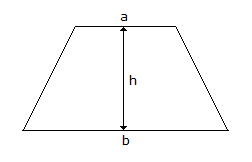
\includegraphics{../data_img/applied-mechanics-and-graphic-statics_1525411410-13.png}
}
\\\begin{enumerate*}[itemjoin=\qquad, label=\Alph*.]
\item{$ \frac{{\text{h}}}{3} \times \frac{{{\text{b}} + {\text{2a}}}}{{{\text{b}} + {\text{a}}}} $}
\item{$ \frac{{\text{h}}}{3} \times \frac{{2{\text{b}} + {\text{a}}}}{{{\text{b}} + {\text{a}}}} $}
\item{$ \frac{{\text{h}}}{2} \times \frac{{{\text{b}} + {\text{2a}}}}{{{\text{b}} + {\text{a}}}} $}
\item{$ \frac{{\text{h}}}{2} \times \frac{{2{\text{b}} + {\text{a}}}}{{{\text{b}} + {\text{a}}}} $}
\end{enumerate*}
\item{The centre of gravity of a quadrant of a circle lies along its central radius at a distance of}
\\\begin{enumerate*}[itemjoin=\qquad, label=\Alph*.]
\item{0.2 R}
\item{0.4 R}
\item{0.3 R}
\item{0.6 R}
\end{enumerate*}
\item{If the angular distance, 0 = 2t\^{}3 - 3t\^{}2, the angular acceleration at t = 1 sec. is
}
\begin{enumerate}[label=\Alph*.]
\item{1 rad/sec\^{}2}
\item{4 rad/sec\^{}2}
\item{6 rad/sec\^{}2}
\item{12 rad/sec\^{}2}
\end{enumerate}
\item{If g\_ 1 and g\_ 2 are the gravitational accelerations on two mountains A and B respectively, the weight of a body when transported from A to B will be multiplied by}
\\\begin{enumerate*}[itemjoin=\qquad, label=\Alph*.]
\item{g\_ 1}
\item{g\_ 2}
\item{$ \frac{{{{\text{g}}_1}}}{{{{\text{g}}_2}}} $}
\item{$ \frac{{{{\text{g}}_2}}}{{{{\text{g}}_1}}} $}
\end{enumerate*}
\item{The vertical reaction at the support `A' of the structure shown in below figure, is \\

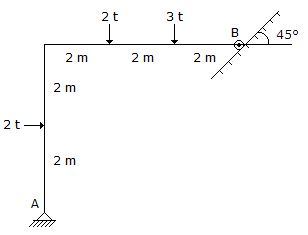
\includegraphics{../data_img/applied-mechanics-and-graphic-statics_1525412526-5.png}
}
\\\begin{enumerate*}[itemjoin=\qquad, label=\Alph*.]
\item{1 t}
\item{2 t}
\item{3 t}
\item{3.5 t}
\end{enumerate*}
\item{The member which does not carry zero force in the structure shown in below figure, is \\

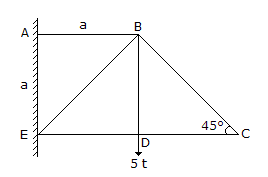
\includegraphics{../data_img/applied-mechanics-and-graphic-statics_1525412688-11.png}
}
\\\begin{enumerate*}[itemjoin=\qquad, label=\Alph*.]
\item{ED}
\item{DC}
\item{BC}
\item{BD}
\end{enumerate*}
\item{The motion of a bicycle wheel is}
\begin{enumerate}[label=\Alph*.]
\item{Translatory}
\item{Rotary}
\item{Rotary and translatory}
\item{Curvilinear}
\end{enumerate}
\item{Dimensional formula of Universal Gravitational constant G is-
}
\begin{enumerate}[label=\Alph*.]
\item{M\^{}-1L\^{}3T\^{}-2}
\item{M\^{}-1L\^{}2T\^{}-2}
\item{M\^{}-2L\^{}3T\^{}-2}
\item{M\^{}-2L\^{}2T\^{}-2}
\end{enumerate}
\item{Effect of a force on a body depends upon its}
\\\begin{enumerate*}[itemjoin=\qquad, label=\Alph*.]
\item{Direction}
\item{Magnitude}
\item{Position}
\item{All the above}
\end{enumerate*}
\item{The following statement is one of the laws of Dynamic friction}
\begin{enumerate}[label=\Alph*.]
\item{The force of friction always acts in a direction opposite to that in which a body is moving}
\item{The magnitude of the kinetic friction bears a constant ratio to the normal reaction between two surfaces. The ratio being slightly less than that in the case of limiting friction}
\item{For moderate speeds the force of friction remains constant but decreases slightly with the increase of speed}
\item{All the above}
\end{enumerate}
\item{If $$l$$ is the span of a light suspension bridge who's each cable carries total weight (w) and the central dip is y, the horizontal pull at each support, is
}
\\\begin{enumerate*}[itemjoin=\qquad, label=\Alph*.]
\item{$ \frac{{{\text{w}}l}}{{4{\text{y}}}} $}
\item{$ \frac{{{\text{w}}l}}{{8{\text{y}}}} $}
\item{$ \frac{{{\text{w}}l}}{{2{\text{y}}}} $}
\item{$ {\text{w}}l $}
\end{enumerate*}
\item{A 49 kg lady stands on a spring scale in an elevator. During the first 5 sec, starting from rest, the scale reads 69 kg. The velocity of the elevator will be}
\\\begin{enumerate*}[itemjoin=\qquad, label=\Alph*.]
\item{10 m/sec}
\item{15 m/sec}
\item{20 m/sec}
\item{25 m/sec}
\end{enumerate*}
\item{Minimum pull in a suspended cable with supports at two ends is equal to}
\begin{enumerate}[label=\Alph*.]
\item{Horizontal thrust}
\item{Support reactions}
\item{Resultant of horizontal thrust and support reaction}
\item{Half the weight of the cable}
\end{enumerate}
\item{Pick up the correct statement from the following. The kinetic energy of a body}
\begin{enumerate}[label=\Alph*.]
\item{Before impact is equal to that after impact}
\item{Before impact is less than that after impact}
\item{Before impact is more than that after impact}
\item{Remain constant}
\end{enumerate}
\item{The force polygon representing a set of forces in equilibrium is a}
\\\begin{enumerate*}[itemjoin=\qquad, label=\Alph*.]
\item{Triangle}
\item{Open polygon}
\item{Closed polygon}
\item{Parallelogram}
\end{enumerate*}
\item{A system of coplanar forces is in equilibrium when}
\begin{enumerate}[label=\Alph*.]
\item{Force polygon closes}
\item{Funicular polygon closes}
\item{Both force polygon" and funicular polygon close}
\item{All the forces are concurrent}
\end{enumerate}
\item{In which of the following trusses, the method of substitution is required for determining the forces in all the members of the truss by graphic statics?}
\begin{enumerate}[label=\Alph*.]
\item{Howe truss}
\item{King post truss}
\item{Fink truss}
\item{Warren truss}
\end{enumerate}
\item{One end of a light string 4 m in length is fixed to a point on a smooth wall and the other end fastened to a point on the surface of a smooth sphere of diameter 2.25 m and of weight 100 kg. The tension in the string is}
\\\begin{enumerate*}[itemjoin=\qquad, label=\Alph*.]
\item{17.5 kg}
\item{19.5 kg}
\item{22.5 kg}
\item{25 kg}
\end{enumerate*}
\item{A weight of 100 kg is supported by a string whose ends are attached to pegs `A' and `B' at the same level shown in below figure. The tension in the string is \\

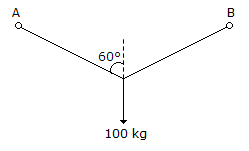
\includegraphics{../data_img/applied-mechanics-and-graphic-statics_1525412734-12.png}
}
\\\begin{enumerate*}[itemjoin=\qquad, label=\Alph*.]
\item{50 kg}
\item{750 kg}
\item{100 kg}
\item{120 kg}
\end{enumerate*}
\item{A 50 kg boy climbs up a 8 m rope in gymnasium in 10 sec. The average power developed by the boy is approximately}
\\\begin{enumerate*}[itemjoin=\qquad, label=\Alph*.]
\item{400 watts}
\item{500 watts}
\item{4000 watts}
\item{None of these}
\end{enumerate*}
\item{Two parallel forces 20 kg and 15 kg act. In order that the distance of the resultant from 20 kg force may be the same as that of the former resultant was from 15 kg, the 20 kg force is diminished by}
\\\begin{enumerate*}[itemjoin=\qquad, label=\Alph*.]
\item{5.5 kg}
\item{6.25 kg}
\item{8.75 kg}
\item{10.5 kg}
\end{enumerate*}
\item{One Newton is equivalent to}
\\\begin{enumerate*}[itemjoin=\qquad, label=\Alph*.]
\item{1 kg. wt}
\item{9.81 kg. wt}
\item{981 dyne}
\item{$ \frac{1}{{9.81}}$$  kg.  $}
\end{enumerate*}
\item{One Joule is equivalent to}
\begin{enumerate}[label=\Alph*.]
\item{9.81 Newton metre}
\item{1 Newton metre}
\item{1 kg wt metre}
\item{1 dyne metre}
\end{enumerate}
\item{A uniform pyramid and a uniform prism of same height lie with their base on the surface. Which is more stable ?}
\begin{enumerate}[label=\Alph*.]
\item{pyramid}
\item{prism}
\item{both equally stable}
\item{none of the above}
\end{enumerate}
\item{`$\mu$' is coefficient of friction. A wheeled vehicle travelling on a circular level track will slip and overturn simultaneously if the ratio of its wheel distance to the height of its centroid, is
}
\\\begin{enumerate*}[itemjoin=\qquad, label=\Alph*.]
\item{$\mu$}
\item{2$\mu$}
\item{3$\mu$}
\item{$ \frac{1}{2} $}
\end{enumerate*}
\item{The unit of moments in M.K.S system, is}
\\\begin{enumerate*}[itemjoin=\qquad, label=\Alph*.]
\item{kg.m}
\item{kg/m\^{}2}
\item{kg/sec\^{}2}
\item{kg/sec}
\end{enumerate*}
\item{One Newton force, is}
\begin{enumerate}[label=\Alph*.]
\item{10\^{}3 dynes}
\item{10\^{}4 dynes}
\item{10\^{}5 dynes}
\item{10\^{}6 dynes}
\end{enumerate}
\item{On a ladder resting on a rough ground and leaning against a smooth vertical wall, the force of friction acts}
\begin{enumerate}[label=\Alph*.]
\item{Downwards at its upper end}
\item{Upwards at its upper end}
\item{Perpendicular to the wall at its upper end}
\item{Zero at its upper end}
\end{enumerate}
\item{On a ladder resisting on a smooth ground and leaning against a rough vertical wall, the force of friction acts}
\begin{enumerate}[label=\Alph*.]
\item{Towards the wall at its upper end}
\item{Away from the wall at its upper end}
\item{Upwards at its upper end}
\item{Downwards at its upper end}
\end{enumerate}
\item{For a given velocity of a projectile, the range is maximum when the angle of projection is}
\\\begin{enumerate*}[itemjoin=\qquad, label=\Alph*.]
\item{30$^\circ$}
\item{45$^\circ$}
\item{90$^\circ$}
\item{0$^\circ$}
\end{enumerate*}
\item{For the given values of initial velocity of projection and angle of inclination of the plane, the maximum range for a projectile projected upwards will be obtained, if the angle of projection is}
\\\begin{enumerate*}[itemjoin=\qquad, label=\Alph*.]
\item{$ \alpha = \frac{\pi }{4} - \frac{\beta }{2} $}
\item{$ \alpha = \frac{\pi }{2} + \frac{\beta }{2} $}
\item{$ \alpha = \frac{\beta }{2} - \frac{\pi }{2} $}
\item{$ \alpha = \frac{\pi }{4} - \frac{\beta }{4} $}
\item{$ \alpha = \frac{\pi }{2} - \frac{\beta }{2} $}
\end{enumerate*}
\item{If $$\alpha $$ is the angular acceleration of a compound pendulum whose angular displacement is $$\theta $$, the frequency of the motion is
}
\\\begin{enumerate*}[itemjoin=\qquad, label=\Alph*.]
\item{$ 2\pi \sqrt {\frac{\alpha }{\theta }}  $}
\item{$ \frac{1}{{2\pi }}\sqrt {\frac{\alpha }{\theta }}  $}
\item{$ 4\pi \sqrt {\frac{\alpha }{\theta }}  $}
\item{$ 2\pi \sqrt {\alpha - \theta }  $}
\end{enumerate*}
\item{In a simple screw jack, the pitch of the screw is 9 mm and length of the handle operating the screw is 45 cm. The velocity ratio of the system is}
\\\begin{enumerate*}[itemjoin=\qquad, label=\Alph*.]
\item{1.5}
\item{5}
\item{25}
\item{314}
\end{enumerate*}
\item{A sphere is resting on two planes BA and BC which are inclined at 45$^\circ$ and 60$^\circ$ respectively with the horizontal. The reaction on the plane BA will be
}
\begin{enumerate}[label=\Alph*.]
\item{Less than that on BC}
\item{More than that of BC}
\item{Equal to that on BC}
\item{None of these}
\end{enumerate}
\item{From the circular plate of a diameter 6 cm is cut out a circular plate whose diameter is equal to radius of the plate. The C.G. of the remainder shifts from the original position through}
\\\begin{enumerate*}[itemjoin=\qquad, label=\Alph*.]
\item{0.25 cm}
\item{0.50 cm}
\item{0.75 cm}
\item{1.00 cm}
\end{enumerate*}
\item{The angles between two forces to make their resultant a minimum and a maximum respectively are}
\\\begin{enumerate*}[itemjoin=\qquad, label=\Alph*.]
\item{0$^\circ$ and 90$^\circ$}
\item{180$^\circ$ and 90$^\circ$}
\item{90$^\circ$ and 180$^\circ$}
\item{180$^\circ$ and 0$^\circ$}
\end{enumerate*}
\item{Time period and length of a second's pendulum respectively are
}
\begin{enumerate}[label=\Alph*.]
\item{1 sec and 99.4 cm}
\item{1 sec and 92.7 cm}
\item{2 sec and 99.4 cm}
\item{2 sec and 92.7 cm}
\end{enumerate}
\item{A cable loaded with 10 kN/m of span is stretched between supports in the same horizontal line 100 m apart. If the central dip is 10 m, then the maximum and minimum pull in the cable respectively are}
\begin{enumerate}[label=\Alph*.]
\item{1346.3 kN and 1500 kN}
\item{1436.2 kN and 1250 kN}
\item{1346.3 kN and 1250 kN}
\item{1436.2 kN and 1500 kN}
\end{enumerate}
\item{When a circular wheel rolls on a straight track, then the shape of body centrode and space centrode respectively are}
\begin{enumerate}[label=\Alph*.]
\item{Straight line and parabola}
\item{Straight line and circle}
\item{Circle and straight line}
\item{Circle and parabola}
\end{enumerate}
\item{Which of the following is a scalar quantity?}
\\\begin{enumerate*}[itemjoin=\qquad, label=\Alph*.]
\item{Energy}
\item{Momentum}
\item{Torque}
\item{Impulse}
\end{enumerate*}
\item{The motion of a particle is described by the relation x = t\^{}2 - 10t + 30, where x is in meters and t in seconds. The total distance travelled by the particle from t = 0 to t = 10 seconds would be
}
\\\begin{enumerate*}[itemjoin=\qquad, label=\Alph*.]
\item{Zero}
\item{30 m}
\item{50 m}
\item{60 m}
\end{enumerate*}
\item{Two forces act an angle of 120$^\circ$. If the greater force is 50 kg and their resultant is perpendicular to the smaller force, the smaller force is
}
\\\begin{enumerate*}[itemjoin=\qquad, label=\Alph*.]
\item{20 kg}
\item{25 kg}
\item{30 kg}
\item{35 kg}
\end{enumerate*}
\item{M.I. of solid sphere, is}
\\\begin{enumerate*}[itemjoin=\qquad, label=\Alph*.]
\item{$ \frac{2}{3}{\text{M}}{{\text{r}}^2} $}
\item{$ \frac{2}{5}{\text{M}}{{\text{r}}^2} $}
\item{$ {\text{M}}{{\text{r}}^2} $}
\item{$ \frac{1}{2}{\text{M}}{{\text{r}}^2} $}
\end{enumerate*}
\item{The following is not a law of static friction:}
\begin{enumerate}[label=\Alph*.]
\item{The force of friction always acts in a direction opposite to that in which the body tends to move}
\item{The force of friction is dependent upon the area of contact}
\item{The force of friction depends upon the roughness of the surface}
\item{The magnitude of the limiting friction bears a constant ratio to the normal reaction between two surfaces}
\end{enumerate}
\item{A hoop of radius 3 m weighs 100 kg. It rolls along a horizontal floor so that at its centre of mass has a speed of 200 mm/sec. The work required to stop the hoop is}
\\\begin{enumerate*}[itemjoin=\qquad, label=\Alph*.]
\item{2 J}
\item{4 J}
\item{6 J}
\item{8 J}
\end{enumerate*}
\item{A satellite moves in its orbit around the earth due to}
\begin{enumerate}[label=\Alph*.]
\item{Gravitational force}
\item{Centripetal force}
\item{Centrifugal force}
\item{None of these}
\end{enumerate}
\item{A satellite goes on moving along its orbit round the earth due to}
\begin{enumerate}[label=\Alph*.]
\item{Gravitational force}
\item{Centrifugal force}
\item{Centripetal force}
\item{None of these}
\end{enumerate}
\item{A bullet weighing 200 g is fired horizontally with a velocity of 25 m/sec from a gun carried on a carriage which together with the gun weighs 100 kg. The velocity of recoil of the gun, will be}
\\\begin{enumerate*}[itemjoin=\qquad, label=\Alph*.]
\item{0.01 m/sec}
\item{0.05 m/sec}
\item{1.00 m/sec}
\item{1.5 m/see}
\end{enumerate*}
\item{Two objects moving with uniform speeds are 5 m apart after 1 second when they move towards each other and are 1 m apart when they move in the same direction. \\
The speeds of the objects are:}
\begin{enumerate}[label=\Alph*.]
\item{2 m/sec and 2 m/sec}
\item{3 m/sec and 2 m/sec}
\item{3 m/sec and 3 m/sec}
\item{4 m/sec and 6 m/sec}
\end{enumerate}
\item{Periodic time of a particle moving with simple harmonic motion is the time taken by the particle for}
\begin{enumerate}[label=\Alph*.]
\item{Half oscillation}
\item{Quarter oscillation}
\item{Complete oscillation}
\item{None of these}
\end{enumerate}
\item{If a particle moves with a uniform angular velocity $$\omega $$ radians/sec along the circumference of a circle of radius r, the equation for the velocity of the particle, is
}
\\\begin{enumerate*}[itemjoin=\qquad, label=\Alph*.]
\item{$ {\text{v}} = \omega \sqrt {{{\text{y}}^2} - {{\text{r}}^2}}  $}
\item{$ \overline {\text{y}} = \omega \sqrt {{\text{y}} - {\text{r}}}  $}
\item{$ {\text{v}} = \omega \sqrt {{{\text{r}}^2} + {{\text{y}}^2}}  $}
\item{$ {\text{v}} = \omega \sqrt {{{\text{r}}^2} - {{\text{y}}^2}}  $}
\end{enumerate*}
\item{A stone is thrown vertically upwards with a vertical velocity of 49 m/sec. It returns to the ground in}
\\\begin{enumerate*}[itemjoin=\qquad, label=\Alph*.]
\item{5 sec}
\item{8 sec}
\item{10 sec}
\item{20 sec}
\end{enumerate*}
\item{A vehicle weighing w kg is to run on a circular curve of radius r. If the height of its centre of gravity above the road level is h and the distance between the centres of wheels is 2a, the maximum velocity, in order to avoid over turning, will be}
\\\begin{enumerate*}[itemjoin=\qquad, label=\Alph*.]
\item{$ \frac{{{\text{gra}}}}{{\text{h}}} $}
\item{$ \sqrt {\frac{{{\text{gra}}}}{{\text{h}}}}  $}
\item{$ \root 3 \of {\frac{{{\text{gra}}}}{{\text{h}}}}  $}
\item{$ \root 4 \of {\frac{{{\text{gra}}}}{{\text{h}}}}  $}
\end{enumerate*}
\item{The unit of force in C.G.S. system of units, is called}
\\\begin{enumerate*}[itemjoin=\qquad, label=\Alph*.]
\item{Dyne}
\item{Newton}
\item{Kg}
\item{All the above}
\end{enumerate*}
\item{A string of length 90 cm is fastened to two points `A' and `B' at the same level 60 cm apart. A ring weighing 120 g is slided on the string. A horizontal force `P' is applied to the ring such that it is in equilibrium vertically below `B'. The value of `P' is:
}
\\\begin{enumerate*}[itemjoin=\qquad, label=\Alph*.]
\item{40 g}
\item{60 g}
\item{80 g}
\item{100 g}
\end{enumerate*}
\item{A body of weight w placed on an inclined plane is acted upon by a force P parallel to the plane which causes the body just to move up the plane. If the angle of inclination of the plane is $$\theta $$ and angle of friction is $$\varphi $$, the minimum value of P, is
}
\\\begin{enumerate*}[itemjoin=\qquad, label=\Alph*.]
\item{$ \frac{{{\text{w}}\sin \left( {\varphi - \theta } \right)}}{{\cos \varphi }} $}
\item{$ \frac{{{\text{w}}\sin \left( {\theta - \varphi } \right)}}{{\cos \varphi }} $}
\item{$ \frac{{{\text{w}}\cos \left( {\theta + \varphi } \right)}}{{\cos \varphi }} $}
\item{$ \frac{{{\text{w}}\sin \theta \cos\left( {\theta - \varphi } \right)}}{{\sin\varphi }} $}
\end{enumerate*}
\item{If the linear velocity of a point on the rim of a wheel of 10 m diameter, is 50 m/sec, its angular velocity will be}
\\\begin{enumerate*}[itemjoin=\qquad, label=\Alph*.]
\item{20 rad/sec}
\item{15 rad/sec}
\item{10 rad/sec}
\item{5 rad/sec}
\end{enumerate*}
\item{The centre of gravity of a trapezoidal dam section whose top width is a, bottom width is b and the vertical side is a, from its vertical face is}
\\\begin{enumerate*}[itemjoin=\qquad, label=\Alph*.]
\item{$ \frac{{{{\text{a}}^2} + {\text{ab}} + {{\text{b}}^2}}}{{3\left( {{\text{a}} + {\text{b}}} \right)}} $}
\item{$ \frac{{{{\text{b}}^2} + {\text{bc}} + {{\text{c}}^2}}}{{3\left( {{\text{b}} + {\text{c}}} \right)}} $}
\item{$ \frac{{{{\text{a}}^2} + {\text{ac}} + {{\text{c}}^2}}}{{3\left( {{\text{a}} + {\text{c}}} \right)}} $}
\item{None of these}
\end{enumerate*}
\item{Pick up the correct statement from the following. A rubber ball when strikes a wall rebounds but a lead ball of same mass and velocity when strikes the same wall, falls down}
\begin{enumerate}[label=\Alph*.]
\item{Rubber and lead balls undergo equal changes in momentum}
\item{Change in momentum suffered by lead ball is less that of rubber ball}
\item{Momentum of rubber ball is less than that of lead ball}
\item{None of these}
\end{enumerate}
\item{If two forces of 3 kg and 4 kg act at right angles to each other, their resultant force will be equal to}
\\\begin{enumerate*}[itemjoin=\qquad, label=\Alph*.]
\item{7 kg}
\item{1 kg}
\item{5 kg}
\item{None of these}
\end{enumerate*}
\item{The masses of two balls are in the ratio of 2 : 1 and their respective velocities are in the ratio of 1 : 2 but in opposite direction before impact. If the coefficient of restitution is $$\frac{1}{2}$$, the velocities of separation of the balls will be equal to
}
\begin{enumerate}[label=\Alph*.]
\item{Original velocity in the same direction}
\item{Half the original velocity in the same direction}
\item{Half the original velocity in the opposite direction}
\item{Original velocity in the opposite direction}
\end{enumerate}
\end{enumerate}
\textbf{Answer Key}
\begin{tabular}{ | c | c c c c c c c c c c | }
\hline
 & 1 & 2 & 3 & 4 & 5 & 6 & 7 & 8 & 9 & 0 \\
\hline
0 & B & A & C & D & D & D & B & A & C & A \\
10 & D & C & D & C & D & C & B & D & D & B \\
20 & C & A & C & C & C & C & C & C & A & C \\
30 & D & B & A & B & A & C & D & C & B & B \\
40 & B & D & B & B & D & C & C & C & A & A \\
50 & B & C & A & B & B & B & B & B & C & D \\
60 & C & B & A & C & B & D & A & D & C & D \\
\hline
\end{tabular}
\clearpage
\subsection*{Section 2}
\begin{enumerate}
\item{When a body of mass M\_ 1 is hanging freely and another of mass M\_ 2 lying on a smooth inclined plane ($$\alpha $$) are connected by a light index tensile string passing over a smooth pulley, the acceleration of the body of mass M\_ 1, will be given by
}
\\\begin{enumerate*}[itemjoin=\qquad, label=\Alph*.]
\item{$ \frac{{{\text{g}}\left( {{{\text{M}}_1} + {{\text{M}}_2}\sin \alpha } \right)}}{{{{\text{M}}_1} + {{\text{M}}_2}}}{\text{m/sec}} $}
\item{$ \frac{{{\text{g}}\left( {{{\text{M}}_1} - {{\text{M}}_2}\sin \alpha } \right)}}{{{{\text{M}}_1} + {{\text{M}}_2}}}{\text{m/se}}{{\text{c}}^2} $}
\item{$ \frac{{{\text{g}}\left( {{{\text{M}}_2} + {{\text{M}}_1}\sin \alpha } \right)}}{{{{\text{M}}_1} + {{\text{M}}_2}}}{\text{m/se}}{{\text{c}}^2} $}
\item{$ \frac{{{\text{g}}\left( {{{\text{M}}_2} \times {{\text{M}}_1}\sin \alpha } \right)}}{{{{\text{M}}_2} - {{\text{M}}_1}}}{\text{m/se}}{{\text{c}}^2} $}
\end{enumerate*}
\item{If two bodies of masses M\_ 1 and M\_ 2(M\_ 1 > M\_ 2) are connected by alight inextensible string passing over a smooth pulley, the tension in the string, will be given by}
\\\begin{enumerate*}[itemjoin=\qquad, label=\Alph*.]
\item{$ {\text{T}} = \frac{{{\text{g}}\left( {{{\text{M}}_1} - {{\text{M}}_2}} \right)}}{{{{\text{M}}_1} + {{\text{M}}_2}}} $}
\item{$ {\text{T}} = \frac{{{\text{g}}\left( {{{\text{M}}_1} + {{\text{M}}_2}} \right)}}{{{{\text{M}}_1} \times {{\text{M}}_2}}} $}
\item{$ {\text{T}} = \frac{{{\text{g}}\left( {{{\text{M}}_2} - {{\text{M}}_1}} \right)}}{{{{\text{M}}_1} + {{\text{M}}_2}}} $}
\item{$ {\text{T}} = \frac{{{\text{g}}\left( {{{\text{M}}_2} + {{\text{M}}_1}} \right)}}{{{{\text{M}}_2} - {{\text{M}}_1}}} $}
\end{enumerate*}
\item{The resultant of the forces acting on a body will be zero if the body}
\begin{enumerate}[label=\Alph*.]
\item{Rotates}
\item{Moves with variable velocity in a straight line}
\item{Moves along a curved path}
\item{Does not move at all}
\end{enumerate}
\item{For a body moving with simple harmonic motion, the number of cycles per second, is known as its}
\\\begin{enumerate*}[itemjoin=\qquad, label=\Alph*.]
\item{Oscillation}
\item{Amplitude}
\item{Periodic time}
\item{Frequency}
\end{enumerate*}
\item{The beam shown in below figure is supported by a hinge at `A' and a roller at `B'. The reaction RA of the hinged support `A' of the beam, is \\

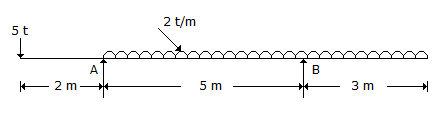
\includegraphics{../data_img/applied-mechanics-and-graphic-statics_1525412791-1.png}
}
\\\begin{enumerate*}[itemjoin=\qquad, label=\Alph*.]
\item{10.8 t}
\item{10.6 t}
\item{10.4 t}
\item{10.2 t}
\end{enumerate*}
\item{One end of an elastic string of natural length `l' and modulus `X' is kept fixed while to the other end is attached a particle of mass m which is hanging freely under gravity. The particle is pulled down vertically through a distance `x', held at rest and then released. \\
The motion is
}
\begin{enumerate}[label=\Alph*.]
\item{A simple harmonic motion}
\item{A rectilinear motion with constant speed}
\item{A damped oscillatory motion}
\item{None of the above}
\end{enumerate}
\item{A bullet weighing 10 gm moves with a velocity of l km/sec. Its kinetic energy is \\
 (i) 5000 Nm \\
 (ii) 5000 kg.m \\
 (iii) 5000 J}
\begin{enumerate}[label=\Alph*.]
\item{Only (ii)}
\item{Both (i) and (iii)}
\item{Both (ii) and (iii)}
\item{All (i), (ii) and (iii)}
\end{enumerate}
\item{The product of mass and velocity of a moving a body, is called}
\\\begin{enumerate*}[itemjoin=\qquad, label=\Alph*.]
\item{Moment}
\item{Momentum}
\item{Power}
\item{Impulse}
\end{enumerate*}
\item{One half of a vibration of a body, is called}
\\\begin{enumerate*}[itemjoin=\qquad, label=\Alph*.]
\item{Period time}
\item{Oscillation}
\item{Beat}
\item{Amplitude}
\end{enumerate*}
\item{The C.G. of the shaded area of the below figure whose curve OM is a parabola from y-axis, is \\

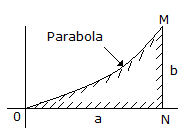
\includegraphics{../data_img/applied-mechanics-and-graphic-statics_1525413129-2.png}
}
\\\begin{enumerate*}[itemjoin=\qquad, label=\Alph*.]
\item{$ \frac{{\text{a}}}{4} $}
\item{$ \frac{{3{\text{a}}}}{4} $}
\item{$ \frac{{3{\text{b}}}}{{10}} $}
\item{$ \frac{{3{\text{a}}}}{{10}} $}
\item{$ \frac{{3{\text{a}}}}{5} $}
\end{enumerate*}
\item{The velocity of a moving body, is}
\begin{enumerate}[label=\Alph*.]
\item{A vector quantity}
\item{A scalar quantity}
\item{A constant quantity}
\item{None of these}
\end{enumerate}
\item{To double the period of oscillation of a simple pendulum}
\begin{enumerate}[label=\Alph*.]
\item{The mass of its bob should be doubled}
\item{The mass of its bob should be quadrupled}
\item{Its length should be quadrupled}
\item{Its length should be doubled}
\end{enumerate}
\item{A particle moves with a velocity of 2 m/sec in a straight line with a negative acceleration of 0.1 m/sec\^{}2. Time required to traverse a distance of 1.5 m, is}
\\\begin{enumerate*}[itemjoin=\qquad, label=\Alph*.]
\item{40 sec}
\item{30 sec}
\item{20 sec}
\item{15 sec}
\end{enumerate*}
\item{The equation of motion of a particle starting from rest along a straight line is x = t\^{}3 - 3t\^{}2 + 5. The ratio of the velocities after 5 sec and 3 sec will be}
\\\begin{enumerate*}[itemjoin=\qquad, label=\Alph*.]
\item{2}
\item{3}
\item{4}
\item{5}
\end{enumerate*}
\item{The equation of motion of a particle starting from rest along a straight line is x = t\^{}3 - 3t\^{}2 + 5. The ratio of the accelerations after 5 sec and 3 sec will be
}
\\\begin{enumerate*}[itemjoin=\qquad, label=\Alph*.]
\item{2}
\item{3}
\item{4}
\item{5}
\end{enumerate*}
\item{A shell of mass 100 kg travelling with a velocity of 10 m/sec breaks into two equal pieces during an explosion which provides an extra kinetic energy of 20000 Joules. If the pieces continue to move in the same direction as before, then the speed of the faster one must be}
\\\begin{enumerate*}[itemjoin=\qquad, label=\Alph*.]
\item{20 m/sec}
\item{30 m/sec}
\item{40 m/sec}
\item{50 m/sec}
\end{enumerate*}
\item{The angular speed of a car while taking a circular turn of radius 100 m at 36 km/hour, is}
\begin{enumerate}[label=\Alph*.]
\item{0.1 radian/sec}
\item{1 radian/sec}
\item{100 radian/sec}
\item{1000 radian/sec}
\end{enumerate}
\item{At the instantaneous center, the velocity of the moving lamina at any instant is}
\\\begin{enumerate*}[itemjoin=\qquad, label=\Alph*.]
\item{Zero}
\item{Maximum}
\item{Minimum}
\item{Varying}
\end{enumerate*}
\item{Which one of the following statements is true?}
\begin{enumerate}[label=\Alph*.]
\item{The tangent of the angle of friction is equal to coefficient of friction}
\item{The angle of repose is equal to angle of friction}
\item{The tangent of the angle of repose is equal to coefficient of friction}
\item{All the above}
\end{enumerate}
\item{A ball is dropped from a height of 16 m on a horizontal floor. If it rebounds to a height of 9 m after striking the floor, the coefficient of restitution between ball and floor is}
\\\begin{enumerate*}[itemjoin=\qquad, label=\Alph*.]
\item{$ \frac{1}{4} $}
\item{$ \frac{2}{3} $}
\item{$ \frac{3}{4} $}
\item{$ \frac{4}{3} $}
\end{enumerate*}
\item{For a non-concurrent force system to be in equilibrium}
\begin{enumerate}[label=\Alph*.]
\item{Only the closure of force polygon is sufficient}
\item{Only the closure of funicular polygon is sufficient}
\item{Both force polygon and funicular polygon must close}
\item{None of the above}
\end{enumerate}
\item{A quantity whose dimensions are M\^{}2L\^{}2T\^{}3 could be the product of}
\begin{enumerate}[label=\Alph*.]
\item{Force and pressure}
\item{Mass and power}
\item{Energy and velocity}
\item{Force and velocity}
\end{enumerate}
\item{The total time of collision and restitution of two bodies, is called}
\begin{enumerate}[label=\Alph*.]
\item{Time of collision}
\item{Period of collision}
\item{Period of impact}
\item{All the above}
\end{enumerate}
\item{When a body slides down an inclined surface, the acceleration (f) of the body, is given by}
\\\begin{enumerate*}[itemjoin=\qquad, label=\Alph*.]
\item{f = g}
\item{f = g sin $\theta$}
\item{f = g cos $\theta$}
\item{f = g tan $\theta$}
\end{enumerate*}
\item{The ratio of the moment of inertia of a rectangle about its centroidal axis to the moment of inertia about its base, is}
\\\begin{enumerate*}[itemjoin=\qquad, label=\Alph*.]
\item{$ \frac{1}{4} $}
\item{$ \frac{1}{2} $}
\item{$ \frac{3}{4} $}
\item{$ 2 $}
\end{enumerate*}
\item{The characteristic of a couple is:}
\begin{enumerate}[label=\Alph*.]
\item{Algebraic sum of forces, constituting a couple is zero}
\item{Algebraic sum of moments of forces, constituting a couple, about any point, is same}
\item{A couple can be never the balanced by a single force}
\item{All the above}
\end{enumerate}
\item{A system of coplanar forces acting on a rigid body can be reduced to}
\begin{enumerate}[label=\Alph*.]
\item{One force only}
\item{One couple only}
\item{One force and one couple only}
\item{None of the above}
\end{enumerate}
\item{The phenomenon of collision of two elastic bodies takes place because bodies}
\begin{enumerate}[label=\Alph*.]
\item{Immediately after collision come momentarily to rest}
\item{Tend to compress each other till they are compressed maximum possible}
\item{Attempt to regain its original shape due to their elasticities}
\item{All the above}
\end{enumerate}
\item{The pole distance is measured in}
\\\begin{enumerate*}[itemjoin=\qquad, label=\Alph*.]
\item{distance scale}
\item{force scale}
\item{mass scale}
\item{time scale}
\end{enumerate*}
\item{The centre of gravity of a plane lamina will not be at its geometrical centre if it is a}
\begin{enumerate}[label=\Alph*.]
\item{Circle}
\item{Equilateral triangle}
\item{Rectangle}
\item{Right angled triangle}
\end{enumerate}
\item{On a mass `m' describing a circular path of radius `r', the centrifugal force
}
\begin{enumerate}[label=\Alph*.]
\item{Acts tangentially to the circular path}
\item{Acts towards the centre of rotation}
\item{Acts away from the centre of rotation}
\item{Is $$\frac{{{\text{m}}{{\text{w}}^{2{\text{r}}}}}}{g}{\text{kfg}}$$}
\end{enumerate}
\item{The condition of equilibrium for any system of forces in a plane is}
\begin{enumerate}[label=\Alph*.]
\item{That polygon of forces must close}
\item{That resultant couple must be zero}
\item{Both (A) and (B)}
\item{None of the above}
\end{enumerate}
\item{The force acting on a point on the surface of a rigid body may be considered to act}
\begin{enumerate}[label=\Alph*.]
\item{At the centre of gravity of the body}
\item{On the periphery of the body}
\item{On any point on the line of action of the force}
\item{At any point on the surface normal to the line of action of the force}
\end{enumerate}
\item{A 2 m long ladder rests against a wall and makes an angle of 30$^\circ$ with the horizontal floor. Where will be the instantaneous center of rotation when the ladder starts slipping ? \\

i. 1.0 in from the wall \\

ii. 1.732 m from the wall \\

iii. 1.0 m above the floor \\

iv. 1.732 m above the floor \\

The correct answer is
}
\\\begin{enumerate*}[itemjoin=\qquad, label=\Alph*.]
\item{(i) and (iii)}
\item{(i) and (iv)}
\item{(ii) and (iii)}
\item{(ii) and (iv)}
\end{enumerate*}
\item{If a body is lying on a plane whose inclination with the horizontal is less than the angle of friction, then \\

i. a force is required to move the body upwards \\

ii. a force is required to move the body downward \\

iii. the body will not be in equilibrium \\

The correct answer is}
\begin{enumerate}[label=\Alph*.]
\item{only (i)}
\item{only (ii)}
\item{both (i) and (ii)}
\item{both (i) and (iii)}
\end{enumerate}
\item{The torque produced by a force depends on \\

i. the magnitude of the force \\

ii. the direction of the force \\

iii. the point of application of the force relative to origin  \\

The correct answer is
}
\begin{enumerate}[label=\Alph*.]
\item{only (i)}
\item{both (i) and (ii)}
\item{both (i) and (iii)}
\item{all (i), (ii) and (iii)}
\end{enumerate}
\item{Select the correct statement}
\begin{enumerate}[label=\Alph*.]
\item{The body centrode rolls on the space centrode}
\item{The space centrode rolls on the body centrode}
\item{Both body and space centrodes may role on each other}
\item{The body centrode never touches space centrode}
\end{enumerate}
\item{The resultant of two forces P and Q is R. If Q is doubled, the new resultant is perpendicular to P. Then,}
\begin{enumerate}[label=\Alph*.]
\item{P = R}
\item{Q = R}
\item{P = Q}
\item{None of the above is correct}
\end{enumerate}
\item{Power developed by a torque, is}
\\\begin{enumerate*}[itemjoin=\qquad, label=\Alph*.]
\item{$ 2\pi {\text{NT kg m/min}} $}
\item{$ \frac{{2\pi {\text{NT}}}}{{4500}}{\text{h}}{\text{.p}}{\text{.}} $}
\item{$ \frac{{2\pi {\text{NT}}}}{{60}}{\text{watts}} $}
\item{All the above}
\end{enumerate*}
\item{The shape of a suspended cable for a uniformly distributed load over it is}
\\\begin{enumerate*}[itemjoin=\qquad, label=\Alph*.]
\item{Circular}
\item{Parabolic}
\item{Catenary}
\item{Cubic parabola}
\end{enumerate*}
\item{A rod AB carries three loads of 30 N, 70 N and 100 N at distances of 20 mm, 90 mm and 150 mm respectively from A. Neglecting the weight of the rod, the point at which the rod will balance is}
\begin{enumerate}[label=\Alph*.]
\item{109.5 mm from A}
\item{119.5 mm from A}
\item{125.5 mm from A}
\item{132.5 mm from A}
\end{enumerate}
\item{The member forces in a statically in determinate truss}
\begin{enumerate}[label=\Alph*.]
\item{Can be obtained by graphic statics}
\item{Cannot be obtained by graphic statics}
\item{May be obtained by graphic statics}
\item{Can be obtained by graphic statics by trial and error}
\end{enumerate}
\item{If v and $$\omega $$ are linear and angular velocities, the centripetal acceleration of a moving body along the circular path of radius r, will be
}
\\\begin{enumerate*}[itemjoin=\qquad, label=\Alph*.]
\item{$ \frac{{\text{r}}}{{{{\text{v}}^2}}} $}
\item{$ \frac{{{{\text{v}}^2}}}{{\text{r}}} $}
\item{$ \frac{{\text{r}}}{{{\omega ^2}}} $}
\item{$ \frac{{{\omega ^2}}}{{\text{r}}} $}
\item{$ {\text{r}}\omega  $}
\end{enumerate*}
\item{To attain the synchronous orbit, the launch of a satellite, is done from a place}
\begin{enumerate}[label=\Alph*.]
\item{On equator}
\item{On 30$^\circ$ latitude}
\item{On 45$^\circ$ latitude}
\item{On the poles}
\end{enumerate}
\item{The rotational velocity of a satellite is increased by 450 m per second if its launch is done from equator}
\\\begin{enumerate*}[itemjoin=\qquad, label=\Alph*.]
\item{Eastward}
\item{Northward}
\item{Westward}
\item{Southward}
\end{enumerate*}
\item{When a body in equilibrium undergoes an infinitely small displacement, work imagined to be done, is known as}
\\\begin{enumerate*}[itemjoin=\qquad, label=\Alph*.]
\item{Imaginary work}
\item{Negative work}
\item{Virtual work}
\item{None of these}
\end{enumerate*}
\item{A ball which is thrown upwards, returns to the ground describing a parabolic path during its flight}
\begin{enumerate}[label=\Alph*.]
\item{Vertical component of velocity remains constant}
\item{Horizontal component of velocity remains constant}
\item{Speed of the ball remains constant}
\item{Kinetic energy of the ball remains constant}
\end{enumerate}
\item{A body A of mass 6.6 kg which is lying on a horizontal platform 4.5 m from its edge is connected to the end of a light string whose other end is supporting a body of mass 3.2 kg as shown in below figure. If the friction between the platform and the body A is $$\frac{1}{3}$$, the acceleration is \\

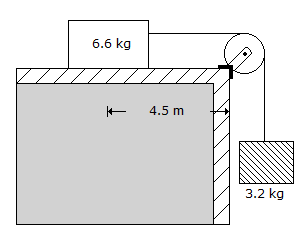
\includegraphics{../data_img/applied-mechanics-and-graphic-statics_1525413218-4.png}
}
\begin{enumerate}[label=\Alph*.]
\item{0.5 m/sec\^{}2}
\item{0.75 m/sec\^{}2}
\item{1.00 m/sec\^{}2}
\item{1.25 m/sec\^{}2}
\end{enumerate}
\item{A cylinder will slip on an inclined plane of inclination angle $$\theta $$ if the coefficient of static friction between plane and cylinder is}
\begin{enumerate}[label=\Alph*.]
\item{less than $$\frac{1}{3}\tan \theta $$}
\item{less than $$\frac{2}{3}\tan \theta $$}
\item{less than $$\frac{1}{3}\sin \theta $$}
\item{less than $$\frac{2}{3}\sin \theta $$}
\end{enumerate}
\item{The following factor affects the orbit of a satellite up to an altitude of 720 km from the earth's surface}
\begin{enumerate}[label=\Alph*.]
\item{Uneven distribution of the gravitational field}
\item{Gravity of the sun and the moon}
\item{Aerodynamic forces}
\item{None of these}
\end{enumerate}
\item{Pick up the incorrect statement from the following. In a simple harmonic motion}
\begin{enumerate}[label=\Alph*.]
\item{Velocity is maximum at its mean position}
\item{Velocity is minimum at the end of the stroke}
\item{Acceleration is minimum at the end of the stroke}
\item{Acceleration is zero at the mean position}
\end{enumerate}
\item{Pick up the incorrect statement from the following. In case of suspension bridge due to rise in temperature,}
\begin{enumerate}[label=\Alph*.]
\item{Dip of the cable increases}
\item{Length of the cable increases}
\item{Dip of the cable decreases}
\item{None of these}
\end{enumerate}
\item{Impulse can be obtained from a}
\begin{enumerate}[label=\Alph*.]
\item{Force-displacement diagram}
\item{Force-time diagram}
\item{Velocity-time diagram}
\item{Velocity-displacement diagram}
\end{enumerate}
\item{The angle of friction is:}
\begin{enumerate}[label=\Alph*.]
\item{The ratio of the friction and the normal reaction}
\item{The force of friction when the body is in motion}
\item{The angle between the normal reaction and the resultant of normal reaction and limiting friction}
\item{The force of friction at which the body is just about to move}
\end{enumerate}
\item{M.I. of a thin ring (external diameter D, internal diameter d) about an axis perpendicular to the plane of the ring, is}
\\\begin{enumerate*}[itemjoin=\qquad, label=\Alph*.]
\item{$ \frac{\pi }{{64}}\left( {{{\text{D}}^4} + {{\text{d}}^4}} \right) $}
\item{$ \frac{\pi }{{32}}\left( {{{\text{D}}^4} - {{\text{d}}^4}} \right) $}
\item{$ \frac{\pi }{{32}}\left( {{{\text{D}}^4} + {{\text{d}}^4}} \right) $}
\item{$ \frac{\pi }{{32}}\left( {{{\text{D}}^4} \times {{\text{d}}^4}} \right) $}
\end{enumerate*}
\item{It is observed that in a certain sinusoidal oscillation, the amplitude is linearly dependent on the frequency f. If the maximum velocity during the oscillation is V, then V must be proportional to}
\\\begin{enumerate*}[itemjoin=\qquad, label=\Alph*.]
\item{f}
\item{$ \frac{1}{{\text{f}}} $}
\item{$ \frac{1}{{{{\text{f}}^2}}} $}
\item{f\^{}2}
\end{enumerate*}
\item{A funicular polygon cannot be made to pass through}
\begin{enumerate}[label=\Alph*.]
\item{One specified point}
\item{Two specified points}
\item{Three specified points}
\item{More than three specified points}
\end{enumerate}
\item{A particle is dropped from the top of a tower 60 m high and another is projected upwards from the foot of the tower to meet the first particle at a height of 15.9 m. The velocity of projection of the second particle is}
\\\begin{enumerate*}[itemjoin=\qquad, label=\Alph*.]
\item{16 m/sec}
\item{18 m/sec}
\item{20 m/sec}
\item{22 m/sec}
\end{enumerate*}
\item{If the angle of projection is double the angle of inclination ($$\alpha $$) of the plane on which particle is projected, the ratio of times of flight up the inclined plane and down the inclined plane, will be
}
\\\begin{enumerate*}[itemjoin=\qquad, label=\Alph*.]
\item{$ \frac{1}{2}\,\cos \alpha  $}
\item{$ \frac{1}{2}\,\sin \alpha  $}
\item{$ \frac{1}{2}\,\tan \alpha  $}
\item{$ 2\cos \alpha  $}
\end{enumerate*}
\item{One end of an elastic string of natural length / and modulus X is kept fixed while to the other end is attached a particle of mass m which is hanging freely under gravity. The particle is pulled down vertically through a distance x, held at rest and then released. The motion is}
\begin{enumerate}[label=\Alph*.]
\item{a simple harmonic motion}
\item{a rectilinear motion with constant speed}
\item{a damped oscillatory motion}
\item{none of the above}
\end{enumerate}
\item{If two forces P and Q (P > Q) act on the same straight line but in opposite direction, their resultant, is}
\\\begin{enumerate*}[itemjoin=\qquad, label=\Alph*.]
\item{P + Q}
\item{$ \frac{{\text{P}}}{{\text{Q}}} $}
\item{$ \frac{{\text{Q}}}{{\text{P}}} $}
\item{P - Q}
\end{enumerate*}
\item{At a given instant ship `A' is travelling at 6 km/h due east and ship `B' is travelling at 8 km/h due north. The velocity of `B' relative to `A' is
}
\\\begin{enumerate*}[itemjoin=\qquad, label=\Alph*.]
\item{7 km/hrs}
\item{2 km/hrs}
\item{1 km/hrs}
\item{10 km/hrs}
\end{enumerate*}
\item{The torque produced by a force depends on \\
 (i) The magnitude of the force \\
 (ii) The direction of the force \\
 (iii) The point of application of the force relative to origin}
\begin{enumerate}[label=\Alph*.]
\item{Only (i)}
\item{Both (i) and (ii)}
\item{Both (i) and (iii)}
\item{All (i), (ii) and (iii)}
\end{enumerate}
\item{If the kinetic energy and potential energy of a simple harmonic oscillator of amplitude A are both equal to half the total energy, then the displacement is equal to}
\\\begin{enumerate*}[itemjoin=\qquad, label=\Alph*.]
\item{$ {\text{A}} $}
\item{$ \frac{{\text{A}}}{2} $}
\item{$ \frac{{\text{A}}}{{\sqrt 2 }} $}
\item{$ {\text{A}}\sqrt 2  $}
\end{enumerate*}
\item{Rate of change of angular momentum is equal to}
\begin{enumerate}[label=\Alph*.]
\item{Force}
\item{Torque}
\item{Linear momentum}
\item{Impulse}
\end{enumerate}
\item{Lami's theorem states that}
\begin{enumerate}[label=\Alph*.]
\item{Three forces acting at a point are always in equilibrium}
\item{If three forces acting on a point can be represented in magnitude and direction by the sides of a triangle, the point will be in the state of equilibrium}
\item{Three coplanar forces acting at a point will be in equilibrium, if each force is proportional to the sine of the angle between the other two}
\item{Three coplanar forces acting at a point will be in equilibrium if each force is inversely proportional to the sine of the angle between the other two}
\end{enumerate}
\item{The maximum frictional force which comes into play, when a body just begins to slide over the surface of a another body, is known}
\begin{enumerate}[label=\Alph*.]
\item{Sliding friction}
\item{Rolling friction}
\item{Limiting friction}
\item{None of these}
\end{enumerate}
\item{A ball moving with a velocity of 5 m/sec impinges a fixed plane at an angle of 45$^\circ$ and its direction after impact is equally inclined to the line of impact. If the coefficient of restitution is 0.5, the velocity of the ball after impact will be
}
\\\begin{enumerate*}[itemjoin=\qquad, label=\Alph*.]
\item{0.5 m/sec}
\item{1.5 m/sec}
\item{2.5 m/sec}
\item{3.5 m/sec}
\end{enumerate*}
\item{A ball of mass 1 kg moving with a velocity of 2 m/sec collides a stationary ball of mass 2 kg and comes to rest after impact. The velocity of the second ball after impact will be}
\\\begin{enumerate*}[itemjoin=\qquad, label=\Alph*.]
\item{Zero}
\item{0.5 m/sec}
\item{1.0 m/sec}
\item{2.0 m/sec}
\end{enumerate*}
\item{The units of inertia of mass are}
\\\begin{enumerate*}[itemjoin=\qquad, label=\Alph*.]
\item{kg/m}
\item{kg/m\^{}2}
\item{m\^{}4}
\item{kg-m\^{}2}
\end{enumerate*}
\end{enumerate}
\textbf{Answer Key}
\begin{tabular}{ | c | c c c c c c c c c c | }
\hline
 & 1 & 2 & 3 & 4 & 5 & 6 & 7 & 8 & 9 & 0 \\
\hline
0 & B & A & D & D & D & A & B & B & C & B \\
10 & A & C & C & D & D & B & A & A & D & C \\
20 & C & B & D & B & A & D & C & D & B & D \\
30 & B & C & C & D & C & D & A & B & D & B \\
40 & A & B & B & A & A & C & B & C & A & D \\
50 & C & C & B & C & B & D & D & C & A & A \\
60 & D & D & D & C & B & C & C & C & C & D \\
\hline
\end{tabular}
\clearpage
\subsection*{Section 3}
\begin{enumerate}
\item{In the structure shown in below figure, the member which carries zero force, is \\

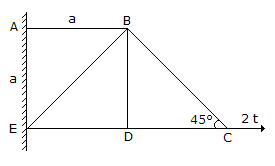
\includegraphics{../data_img/applied-mechanics-and-graphic-statics_1525413392-7.png}
}
\\\begin{enumerate*}[itemjoin=\qquad, label=\Alph*.]
\item{AB}
\item{BC}
\item{BE}
\item{All the above}
\end{enumerate*}
\item{If two equal forces of magnitude P act at an angle $$\theta $$, their resultant, will be
}
\\\begin{enumerate*}[itemjoin=\qquad, label=\Alph*.]
\item{$ {\text{P}}\cos \frac{\theta }{2} $}
\item{$ 2{\text{P}}\sin\frac{\theta }{2} $}
\item{$ {\text{P}}\tan\frac{\theta }{2} $}
\item{$ 2{\text{P}}\cos \frac{\theta }{2} $}
\end{enumerate*}
\item{A projectile is thrown at an angle `$\alpha$' to the horizontal with velocity `v'. It will have the maximum centripetal acceleration
}
\begin{enumerate}[label=\Alph*.]
\item{At the start}
\item{At the top of the trajectory}
\item{As it strikes the ground}
\item{Elsewhere}
\end{enumerate}
\item{Varingon's theorem of moment's states
}
\begin{enumerate}[label=\Alph*.]
\item{Arithmetical sum of the moments of two forces about any point, is equal to the moments of their resultant about that point}
\item{Algebraic sum of the moments of two forces about any point, is equal to the moment of their resultant about that point}
\item{Arithmetical sum of the moments of the forces about any point in their plane, is equal to the moment of their resultant about that point}
\item{Algebraic sum of the moments of the forces about any point in their plane, is equal to the moment of their resultant about that point}
\end{enumerate}
\item{The resultant of two forces acting at right angles is 5 kgf and if they act at an angle of 60$^\circ$, it is 37 kgf. The magnitudes of the forces are:
}
\\\begin{enumerate*}[itemjoin=\qquad, label=\Alph*.]
\item{2 kgf, 3 kgf}
\item{3 kgf, 4 kgf}
\item{4 kgf, 5 kgf}
\item{5 kgf, 3 kgf}
\end{enumerate*}
\item{A particle is executing simple harmonic motion in a line 1.0 m long. If the time of one complete vibration is 1 sec, then the maximum velocity of the particle is}
\\\begin{enumerate*}[itemjoin=\qquad, label=\Alph*.]
\item{1.00 m/sec}
\item{1.57 m/sec}
\item{3.14 m/sec}
\item{6.28 m/sec}
\end{enumerate*}
\item{If A is the amplitude of particle executing simple harmonic motion, then the total energy E of the particle is}
\begin{enumerate}[label=\Alph*.]
\item{Proportional to A}
\item{Proportional to A\^{}2}
\item{Proportional to $$\frac{1}{{{{\text{A}}^2}}}$$}
\item{Independent of A}
\end{enumerate}
\item{If A is the amplitude of particle executing simple harmonic motion, then the total energy E of the particle is}
\begin{enumerate}[label=\Alph*.]
\item{proportional to A}
\item{proportional to A\^{}2}
\item{proportional to $$\frac{1}{{{{\text{A}}^2}}}$$}
\item{independent of A}
\end{enumerate}
\item{`P' is the force acting on a body whose mass is `m' and acceleration is `f'. The equation P - mf= 0, is known as
}
\begin{enumerate}[label=\Alph*.]
\item{Equation of dynamics}
\item{Equation of dynamic equilibrium}
\item{Equation of statics}
\item{None of these}
\end{enumerate}
\item{For lifting a load of 50 kg through a distance of 2.5 cm, an effort of 12.5 kg is moved through a distance of 40 cm. The efficiency of the lifting machine, is}
\\\begin{enumerate*}[itemjoin=\qquad, label=\Alph*.]
\item{60 \%}
\item{65 \%}
\item{70 \%}
\item{75 \%}
\end{enumerate*}
\item{The angle which an inclined surface makes with the horizontal when a body placed on it is on the point of moving down, is called}
\begin{enumerate}[label=\Alph*.]
\item{Angle of repose}
\item{Angle of friction}
\item{Angle of inclination}
\item{None of these}
\end{enumerate}
\item{The resultant of two forces acting at right angles is $$\sqrt {34} \,$$ kg and acting at 60$^\circ$ is 70 kg. The forces are
}
\\\begin{enumerate*}[itemjoin=\qquad, label=\Alph*.]
\item{1 kg and 4 kg}
\item{2 kg and 3 kg}
\item{$ \sqrt 3 $$ kg and $$\sqrt 5 $$  $}
\item{3 kg and 5 kg}
\end{enumerate*}
\item{The moment of inertia of a circular lamina of diameter `d', about an axis perpendicular to the plane of the lamina and passing through its centre, is
}
\\\begin{enumerate*}[itemjoin=\qquad, label=\Alph*.]
\item{$ \frac{{\pi {{\text{d}}^4}}}{{12}} $}
\item{$ \frac{{\pi {{\text{d}}^4}}}{{16}} $}
\item{$ \frac{{\pi {{\text{d}}^4}}}{{24}} $}
\item{$ \frac{{\pi {{\text{d}}^4}}}{{32}} $}
\item{$ \frac{{\pi {{\text{d}}^4}}}{{36}} $}
\end{enumerate*}
\item{A circular disc rotates at n rpm. The angular velocity of a circular ring of same mass and radius as the disc and to have the same angular momentum is}
\\\begin{enumerate*}[itemjoin=\qquad, label=\Alph*.]
\item{n rpm}
\item{$ \frac{{\text{n}}}{2}$$ r $}
\item{$ \frac{{\text{n}}}{4}$$ r $}
\item{2n rpm}
\end{enumerate*}
\item{Instantaneous center is at infinity when the angular velocity is}
\\\begin{enumerate*}[itemjoin=\qquad, label=\Alph*.]
\item{Constant}
\item{Zero}
\item{Maximum}
\item{Minimum}
\end{enumerate*}
\item{A disc of mass 4 kg, radius 0.5 m and moment of inertia 3 kg.m\^{}2 rolls on a horizontal surface so that its center moves with speed 5 m/see. Kinetic energy of the disc is
}
\\\begin{enumerate*}[itemjoin=\qquad, label=\Alph*.]
\item{50 J}
\item{150 J}
\item{200 J}
\item{400 J}
\end{enumerate*}
\item{A cable loaded with 0.5 tonne per horizontal metre span is stretched between supports in the same horizontal line 400 m apart. If central dip is 20 m, the minimum tension in the cable, will be}
\begin{enumerate}[label=\Alph*.]
\item{200 tonnes at the centre}
\item{500 tonnes at the centre}
\item{200 tonnes at the right support}
\item{200 tonnes at the left support}
\end{enumerate}
\item{A simple pendulum of length L has an energy E when its amplitude is A. If its amplitude is increased to 2A, the energy becomes}
\\\begin{enumerate*}[itemjoin=\qquad, label=\Alph*.]
\item{E}
\item{$ \frac{{\text{E}}}{2} $}
\item{2E}
\item{4E}
\end{enumerate*}
\item{A simple pendulum of length L has an energy E, when its amplitude is A. If the length of pendulum is doubled, the energy will be}
\\\begin{enumerate*}[itemjoin=\qquad, label=\Alph*.]
\item{E}
\item{$ \frac{{\text{E}}}{2} $}
\item{2E}
\item{4E}
\end{enumerate*}
\item{If the horizontal range is 2.5 times the greatest height, the angle of projection of the projectile, is}
\\\begin{enumerate*}[itemjoin=\qquad, label=\Alph*.]
\item{57$^\circ$}
\item{58$^\circ$}
\item{59$^\circ$}
\item{60$^\circ$}
\end{enumerate*}
\item{The units of moment of inertia of an area are}
\\\begin{enumerate*}[itemjoin=\qquad, label=\Alph*.]
\item{kg/m}
\item{kg/m\^{}2}
\item{m\^{}4}
\item{m\^{}3}
\end{enumerate*}
\item{A flywheel of moment of inertia 20 kg.m is acted upon by a tangential force of 5 N at 2 m from its axis, for 3 seconds. The increase in angular velocity in radian per second is}
\\\begin{enumerate*}[itemjoin=\qquad, label=\Alph*.]
\item{$ \frac{1}{2} $}
\item{$ \frac{3}{2} $}
\item{2}
\item{3}
\end{enumerate*}
\item{The maximum velocity of a body vibrating with a simple harmonic motion of amplitude 150 mm and frequency 2 vibrations/sec, is}
\\\begin{enumerate*}[itemjoin=\qquad, label=\Alph*.]
\item{188.5 m/sec}
\item{18.85 m/sec}
\item{1.885 m/sec}
\item{0.18845 m/sec}
\end{enumerate*}
\item{A ball moving on a smooth horizontal table hits a rough vertical wall, the coefficient of restitution between ball and wall being $$\frac{1}{3}$$. The ball rebounds at the same angle. The fraction of its kinetic energy lost is}
\\\begin{enumerate*}[itemjoin=\qquad, label=\Alph*.]
\item{$ \frac{1}{3} $}
\item{$ \frac{2}{3} $}
\item{$ \frac{1}{9} $}
\item{$ \frac{8}{9} $}
\end{enumerate*}
\item{For a self-locking machine, the efficiency should be}
\\\begin{enumerate*}[itemjoin=\qquad, label=\Alph*.]
\item{Less than 60\%}
\item{50\%}
\item{More than 50\%}
\item{None of these}
\end{enumerate*}
\item{The condilion for a lifting machine to be reversible is that its efficiency should be}
\begin{enumerate}[label=\Alph*.]
\item{less than 50\%}
\item{more than 50\%}
\item{more than 66.67\%}
\item{equal to 100\%}
\end{enumerate}
\item{Coefficient of friction depends on}
\begin{enumerate}[label=\Alph*.]
\item{Nature of surfaces only}
\item{Area of contact only}
\item{Both (A) and (B)}
\item{None of the above}
\end{enumerate}
\item{The ratio of the speed of a rolling cylinder to the speed of sliding cylinder is}
\begin{enumerate}[label=\Alph*.]
\item{Less than 1}
\item{Equal to 1}
\item{Between 1 and 2}
\item{Greater than 2}
\end{enumerate}
\item{A load of 500 kg was lifted through a distance of 13 cm. by an effort of 25 kg which moved through a distance of 650 cm. The mechanical advantage of the lifting machine is}
\\\begin{enumerate*}[itemjoin=\qquad, label=\Alph*.]
\item{15}
\item{18}
\item{20}
\item{26}
\end{enumerate*}
\item{A load of 500 kg was lifted through a distance of 13 cm. by an effort of 25 kg which moved through a distance of 650 cm. The velocity ratio of the lifting machine is}
\\\begin{enumerate*}[itemjoin=\qquad, label=\Alph*.]
\item{50}
\item{55}
\item{60}
\item{65}
\end{enumerate*}
\item{A load of 500 kg was lifted through a distance of 13 cm. by an effort of 25 kg which moved through a distance of 650 cm. The efficiency of the lifting machine is}
\\\begin{enumerate*}[itemjoin=\qquad, label=\Alph*.]
\item{50 \%}
\item{40 \%}
\item{55 \%}
\item{30 \%}
\end{enumerate*}
\item{A projectile is fired with a velocity of 100.3 m/sec. at an elevation of 60$^\circ$. The velocity attained by the projectile when it is moving at a height of 100 m, is
}
\\\begin{enumerate*}[itemjoin=\qquad, label=\Alph*.]
\item{70 m/sec}
\item{75 m/sec}
\item{80 m/sec}
\item{90 m/sec}
\end{enumerate*}
\item{A weight `W' is suspended at the free end of a light member hinged to a vertical wall. If the angle of inclination of the member with the upper wall is $\theta$$^\circ$, the force introduced in the member, is
}
\\\begin{enumerate*}[itemjoin=\qquad, label=\Alph*.]
\item{W sec $\theta$}
\item{W cos $\theta$}
\item{W sin $\theta$}
\item{W cosec $\theta$}
\end{enumerate*}
\item{A stone of mass 1 kg is tied to a string of length 1 m and whirled in a horizontal circle at a constant angular speed 5 rad/sec. The tension in the string is,}
\\\begin{enumerate*}[itemjoin=\qquad, label=\Alph*.]
\item{5 N}
\item{10 N}
\item{15 N}
\item{25 N}
\end{enumerate*}
\item{Two loads of 50 kg and 75 kg are hung at the ends of a rope passing over a smooth pulley shown in below figure. The tension in the string is: \\

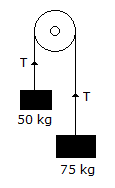
\includegraphics{../data_img/applied-mechanics-and-graphic-statics_1525413496-9.png}
}
\\\begin{enumerate*}[itemjoin=\qquad, label=\Alph*.]
\item{50 kg}
\item{75 kg}
\item{25 kg}
\item{60 kg}
\end{enumerate*}
\item{If the direction of projection bisects the angle between the vertical and the inclined plane, then the range of projectile on the inclined plane is}
\\\begin{enumerate*}[itemjoin=\qquad, label=\Alph*.]
\item{Zero}
\item{Maximum}
\item{Minimum}
\item{None of these}
\end{enumerate*}
\item{Williot-Mohr diagram is used to determine deflection in}
\begin{enumerate}[label=\Alph*.]
\item{Trusses only}
\item{Beam only}
\item{Rigid frames only}
\item{Any type of structure}
\end{enumerate}
\item{Total no of instantaneous centers of a machine having `n' links, is
}
\\\begin{enumerate*}[itemjoin=\qquad, label=\Alph*.]
\item{$ \frac{{\text{n}}}{2} $}
\item{n}
\item{(n - 1)}
\item{$ \frac{{{\text{n}}\left( {{\text{n}} - 1} \right)}}{2} $}
\end{enumerate*}
\item{The acceleration of a train starting from rest at any instant is $$\frac{1}{{6\left( {{\text{V}} + 1} \right)}}{\text{m/se}}{{\text{c}}^2}$$ ~ ~where `V' is the velocity of the train in m/sec. The train will attain a velocity of 36 km/hour after travelling a distance of
}
\\\begin{enumerate*}[itemjoin=\qquad, label=\Alph*.]
\item{2000 m}
\item{2100 m}
\item{2200 m}
\item{2300 m}
\item{2500 m}
\end{enumerate*}
\item{A particle moves in a straight line and its position is defined by the equation x = 6t\^{}2 - t\^{}3 where t is expressed in seconds and `x' in meters. The maximum velocity during the motion is
}
\\\begin{enumerate*}[itemjoin=\qquad, label=\Alph*.]
\item{6 m/sec}
\item{12 m/sec}
\item{24 m/sec}
\item{48 m/sec}
\end{enumerate*}
\item{The ends of a string weighing w/metre are attached to two points at the same horizontal level. If the central dip is very small, the horizontal tension of the string throughout is}
\\\begin{enumerate*}[itemjoin=\qquad, label=\Alph*.]
\item{$ \frac{{{\text{w}}l}}{{4{\text{d}}}} $}
\item{$ \frac{{{\text{w}}{l^2}}}{{4{\text{d}}}} $}
\item{$ \frac{{{\text{w}}{l^2}}}{{8{\text{d}}}} $}
\item{$ \frac{{{\text{w}}{l^2}}}{{16{\text{d}}}} $}
\end{enumerate*}
\item{A rope is wrapped twice around a rough pole with a coefficient of friction $$\mu $$ . It is subjected to a force F\_ 1 at one end and a gradually increasing force F\_ 2 is applied at the other end till the rope just starts slip-ping. At this instant the ratio of F\_ 2 to F\_ 1 is
}
\\\begin{enumerate*}[itemjoin=\qquad, label=\Alph*.]
\item{$ 1 $}
\item{$ {{\text{e}}^{4\pi \mu }} $}
\item{$ {{\text{e}}^{2\mu }} $}
\item{$ {{\text{e}}^{360\mu }} $}
\end{enumerate*}
\item{If two forces acting at a point are in equilibrium, they must be equal in magnitude and their line of action must be along}
\begin{enumerate}[label=\Alph*.]
\item{The same line in the same sense}
\item{The same line in opposite sense}
\item{The perpendicular to both the lines}
\item{None of these}
\end{enumerate}
\item{Force polygon method is applicable for}
\begin{enumerate}[label=\Alph*.]
\item{Any coplanar force system}
\item{A system of parallel forces only}
\item{Concurrent coplanar force system}
\item{Non-concurrent coplanar force system}
\end{enumerate}
\item{Force polygon method is applicable for}
\begin{enumerate}[label=\Alph*.]
\item{any copianar force system}
\item{a system of parallel forces only}
\item{concurrent copianar force system}
\item{non-concurrent copianar force system}
\end{enumerate}
\item{From a solid cylinder of height 8 cm and radius 4 cm, a right circular cone is scooped out on the same base and having the same height as that of the cylinder. The C.G. of the remainder is at a height of}
\\\begin{enumerate*}[itemjoin=\qquad, label=\Alph*.]
\item{4.5 cm}
\item{5.0 cm}
\item{5.25 cm}
\item{5.5 cm}
\end{enumerate*}
\item{The unit of impulse, is}
\begin{enumerate}[label=\Alph*.]
\item{kg.m/sec}
\item{kg.m/sec\^{}3}
\item{kg.m/sec\^{}2}
\item{kg.m\^{}2/sec}
\end{enumerate}
\item{The gravitational force makes a satellite go round the earth in a circular orbit, if it is projected with an initial velocity of}
\begin{enumerate}[label=\Alph*.]
\item{8.04 km/sec at a height of 285 km}
\item{11.11 km/sec at a height of 37,400 km}
\item{11.26 km/sec, the satellite escapes the pull of the earth}
\item{All the above}
\end{enumerate}
\item{Two circular discs of same weight and thickness are made from metals having different densities. Which disc will have the larger rotational inertia about its central axis?}
\begin{enumerate}[label=\Alph*.]
\item{Disc with larger density}
\item{Disc with smaller density}
\item{Both discs will have same rotational inertia}
\item{None of the above}
\end{enumerate}
\item{A rod 5 m in length is moving in a vertical plane. When it is inclined at 60$^\circ$ to horizontal, its lower end is moving horizontally at 3 m/sec and upper end is moving in vertical direction. The velocity of its upper end, is
}
\\\begin{enumerate*}[itemjoin=\qquad, label=\Alph*.]
\item{0.5 m/sec}
\item{1.0 m/sec}
\item{1.5 m/sec}
\item{2.5 m/sec}
\end{enumerate*}
\item{The ratio of kinetic energy and potential energy of a simple harmonic oscillator, at a displacement equal to half its amplitude is given by}
\\\begin{enumerate*}[itemjoin=\qquad, label=\Alph*.]
\item{1 : 2}
\item{1 : 1}
\item{2 : 1}
\item{3 : 1}
\end{enumerate*}
\item{Newton's law of Collision of elastic bodies states that when two moving bodies collide each other, their velocity of separation}
\begin{enumerate}[label=\Alph*.]
\item{Is directly proportional to their velocity of approach}
\item{Is inversely proportional to their velocity of approach}
\item{Bears a constant ratio to their velocity of approach}
\item{Is equal to the sum of their velocities of approach}
\end{enumerate}
\item{A quantity measured in the C.G.S system of units has dimensions M''2L3 T3/2. What numerical factor would be required to convert the quantity to SI units ?
}
\\\begin{enumerate*}[itemjoin=\qquad, label=\Alph*.]
\item{1}
\item{100}
\item{1/100}
\item{1/10000}
\end{enumerate*}
\item{The necessary condition of equilibrium of a body is:}
\begin{enumerate}[label=\Alph*.]
\item{Algebraic sum of horizontal components of all the forces must be zero}
\item{Algebraic sum of vertical components of all the forces must be zero}
\item{Algebraic sum of the moments of the forces about a point must be zero}
\item{All (A), (B) and (C)}
\end{enumerate}
\item{The resolved part of the resultant of two forces inclined at an angle $\theta$ in a given direction is
}
\begin{enumerate}[label=\Alph*.]
\item{Algebraic sum of the resolved parts of the forces in the direction}
\item{Arithmetical sum of the resolved parts of the forces in the direction}
\item{Difference of the forces multiplied by cosine $\theta$$^\circ$}
\item{Sum of the forces multiplied by the tangent $\theta$$^\circ$}
\end{enumerate}
\item{When a body moves round a fixed axis, it has}
\begin{enumerate}[label=\Alph*.]
\item{A rotary motion}
\item{A circular motion}
\item{A translatory}
\item{A rotary motion and translatory motion}
\end{enumerate}
\item{Time of flight of a projectile on a horizontal plane, is}
\\\begin{enumerate*}[itemjoin=\qquad, label=\Alph*.]
\item{$ \frac{{2{\text{u}}\sin \alpha }}{{\text{g}}} $}
\item{$ \frac{{2{\text{u}}\cos \alpha }}{{\text{g}}} $}
\item{$ \frac{{2{\text{u}}\tan \alpha }}{{\text{g}}} $}
\item{$ \frac{{2{\text{u}}\cot \alpha }}{{\text{g}}} $}
\end{enumerate*}
\item{If the velocity of projection is 4 m/sec and the angle of projection is $${\alpha ^ \circ }$$, the maximum height of the projectile from a horizontal plane, is
}
\\\begin{enumerate*}[itemjoin=\qquad, label=\Alph*.]
\item{$ \frac{{{{\text{u}}^2}{{\cos }^2}\alpha }}{{2{\text{g}}}} $}
\item{$ \frac{{{{\text{u}}^2}{{\sin }^2}\alpha }}{{2{\text{g}}}} $}
\item{$ \frac{{{{\text{u}}^2}{{\tan }^2}\alpha }}{{2{\text{g}}}} $}
\item{$ \frac{{{{\text{u}}^2}\sin2\alpha }}{{2{\text{g}}}} $}
\end{enumerate*}
\item{Two particles have been projected at angles 64$^\circ$ and 45$^\circ$ to the horizontal. If the velocity of projection of first is 10 m/sec, the velocity of projection of the other for equal horizontal ranges is
}
\\\begin{enumerate*}[itemjoin=\qquad, label=\Alph*.]
\item{9.3 m/sec}
\item{8.3 m/sec}
\item{7.3 m/sec}
\item{6.3 m/sec}
\end{enumerate*}
\item{For maximum range of a projectile, the angle of projection should be}
\\\begin{enumerate*}[itemjoin=\qquad, label=\Alph*.]
\item{30$^\circ$}
\item{45$^\circ$}
\item{60$^\circ$}
\item{None of these}
\end{enumerate*}
\item{If the angle between the applied force and the direction of motion of a body, is between 90$^\circ$ and 180$^\circ$, the work done, is called
}
\\\begin{enumerate*}[itemjoin=\qquad, label=\Alph*.]
\item{Virtual work}
\item{Imaginary work}
\item{Zero work}
\item{Negative work}
\end{enumerate*}
\item{A particle of mass 2 kg executes simple harmonic motion of frequency 6/71 Hz and amplitude 0.25 m. Its maximum kinetic energy is}
\\\begin{enumerate*}[itemjoin=\qquad, label=\Alph*.]
\item{4.5 J}
\item{9.0 J}
\item{12.0 J}
\item{18.0 J}
\end{enumerate*}
\item{A particle is dropped from a height of 3 m on a horizontal floor, which has a coefficient of restitution with the ball of $$\frac{1}{2}$$. The height to which the ball will rebound after striking the floor is}
\\\begin{enumerate*}[itemjoin=\qquad, label=\Alph*.]
\item{0.5 m}
\item{0.75 m}
\item{1.0 m}
\item{1.5 m}
\end{enumerate*}
\item{A glass ball is shot to hit a wall from a point on a smooth floor. If the ball returns back to the point of projection in twice the time taken in reaching the wall, the coefficient of restitution between the glass ball and the wall is}
\\\begin{enumerate*}[itemjoin=\qquad, label=\Alph*.]
\item{0.25}
\item{0.33}
\item{0.40}
\item{0.50}
\end{enumerate*}
\item{For the system of the loads shown in bellow figure, the time required for the 6.6 kg load to fall on the edge, is \\

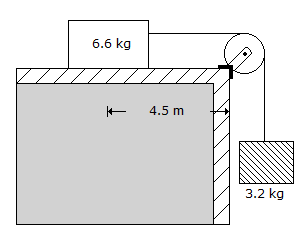
\includegraphics{../data_img/applied-mechanics-and-graphic-statics_1525414366-4.png}
}
\\\begin{enumerate*}[itemjoin=\qquad, label=\Alph*.]
\item{1 sec}
\item{2 sec}
\item{3 sec}
\item{4 sec}
\end{enumerate*}
\item{The moment of inertia of a triangular section (base b, height h) about centroidal axis parallel to the base, is}
\\\begin{enumerate*}[itemjoin=\qquad, label=\Alph*.]
\item{$ \frac{{{{\text{b}}^3}{\text{h}}}}{{12}} $}
\item{$ \frac{{{\text{b}}{{\text{h}}^3}}}{3} $}
\item{$ \frac{{{\text{b}}{{\text{h}}^3}}}{{36}} $}
\item{$ \frac{{{\text{b}}{{\text{h}}^3}}}{2} $}
\end{enumerate*}
\item{The point about which combined motion of rotation and translation of a rigid body takes place, is known as}
\begin{enumerate}[label=\Alph*.]
\item{Virtual centre}
\item{Instantaneous centre}
\item{Instantaneous axis}
\item{Point of rotation}
\end{enumerate}
\item{Newton's Law of Motion is:
}
\begin{enumerate}[label=\Alph*.]
\item{Everybody continues in its state of rest or of uniform motion in a straight line, unless it is acted upon by some external force}
\item{The rate of change of momentum is directly proportional to the impressed force, and takes place in the same direction, in which the force acts}
\item{To every action, there is always an equal and opposite reaction}
\item{All the above}
\end{enumerate}
\item{Joule is the unit of}
\\\begin{enumerate*}[itemjoin=\qquad, label=\Alph*.]
\item{Power}
\item{Impulse}
\item{Work}
\item{Momentum}
\end{enumerate*}
\item{Joule is the unit of}
\\\begin{enumerate*}[itemjoin=\qquad, label=\Alph*.]
\item{Work}
\item{Force}
\item{Power}
\item{Torque}
\end{enumerate*}
\end{enumerate}
\textbf{Answer Key}
\begin{tabular}{ | c | c c c c c c c c c c | }
\hline
 & 1 & 2 & 3 & 4 & 5 & 6 & 7 & 8 & 9 & 0 \\
\hline
0 & D & D & A & D & B & C & B & B & A & D \\
10 & A & D & D & B & B & C & B & D & B & B \\
20 & C & B & C & D & A & B & A & A & C & A \\
30 & B & D & A & D & D & B & A & D & D & B \\
40 & C & B & B & C & C & B & A & D & B & B \\
50 & D & C & A & D & A & B & A & B & A & B \\
60 & D & B & B & D & C & C & B & D & C & A \\
\hline
\end{tabular}
\\\textbf{Explanation}\\
31.
Mechanical advantage (MA) = Load (W)/Effort (P).
\clearpage
\subsection*{Section 4}
\begin{enumerate}
\item{A block of weight 50 kg is placed on a horizontal plane. When a horizontal force of 18 kg is applied, the block is just on the point of motion. The angle of friction is}
\\\begin{enumerate*}[itemjoin=\qquad, label=\Alph*.]
\item{17$^\circ$ 48'}
\item{18$^\circ$ 48'}
\item{19$^\circ$ 48'}
\item{20$^\circ$ 48'}
\end{enumerate*}
\item{In a simple harmonic motion, the position of equilibrium is always}
\begin{enumerate}[label=\Alph*.]
\item{Stable}
\item{Unstable}
\item{Neutral}
\item{None of the above}
\end{enumerate}
\item{The velocity ratio of an inclined plane of inclination `$\theta$' with horizontal for lifting a load is
}
\\\begin{enumerate*}[itemjoin=\qquad, label=\Alph*.]
\item{sin $\theta$}
\item{cos $\theta$}
\item{tan $\theta$}
\item{cosec $\theta$}
\end{enumerate*}
\item{The maximum displacement of a particle executing S.H.M. corresponds to}
\begin{enumerate}[label=\Alph*.]
\item{Zero potential energy and maximum kinetic energy}
\item{Zero kinetic energy and maximum potential energy}
\item{Maximum kinetic energy and maximum potential energy}
\item{Minimum kinetic energy and minimum potential energy}
\end{enumerate}
\item{A force P of 50 N and another force Q of unknown magnitude act at 90$^\circ$ to each other. They are balanced by a force of 130 N. The magnitude of Q is
}
\\\begin{enumerate*}[itemjoin=\qquad, label=\Alph*.]
\item{60 N}
\item{80 N}
\item{100 N}
\item{120 N}
\end{enumerate*}
\item{If two forces each equal to `T' in magnitude act at right angles, their effect may be neutralized by a third force acting along their bisector in opposite direction whose magnitude will be
}
\\\begin{enumerate*}[itemjoin=\qquad, label=\Alph*.]
\item{2T}
\item{$ \frac{1}{2}{\text{T}} $}
\item{$ \sqrt 2 {\text{ T}} $}
\item{3T}
\end{enumerate*}
\item{If a particle is projected inside a horizontal tunnel which is 554 cm high with a velocity of 60 m per sec, the angle of projection for maximum range, is}
\\\begin{enumerate*}[itemjoin=\qquad, label=\Alph*.]
\item{8$^\circ$}
\item{9$^\circ$}
\item{10$^\circ$}
\item{11$^\circ$}
\end{enumerate*}
\item{Kinetic friction may be defined as}
\begin{enumerate}[label=\Alph*.]
\item{Friction force acting when the body is just about to move}
\item{Friction force acting when the body is in motion}
\item{Angle between normal reaction and resultant of normal reaction and limiting friction}
\item{Ratio of limiting friction and normal reaction}
\end{enumerate}
\item{Energy may be defined as}
\begin{enumerate}[label=\Alph*.]
\item{Power of doing work}
\item{Capacity of doing work}
\item{Rate of doing work}
\item{All the above}
\end{enumerate}
\item{A projectile has maximum range of 40 m on a horizontal plane. If angle of projection is a and the time of flight is 1 second, then sin a must be about (Assume g = 10 m/sec\^{}2)
}
\\\begin{enumerate*}[itemjoin=\qquad, label=\Alph*.]
\item{$ \frac{1}{4} $}
\item{$ \frac{1}{3} $}
\item{$ \frac{1}{2} $}
\item{$ \frac{1}{5} $}
\end{enumerate*}
\item{A car goes round a curve of radius 100 m at 25 m/sec. The angle to the horizontal at which the road must be banked to prevent sideways friction on the car wheels is tan\^{}-1x, where x is (Assume g = 10 m/sec\^{}2)
}
\\\begin{enumerate*}[itemjoin=\qquad, label=\Alph*.]
\item{$ \frac{3}{8} $}
\item{$ \frac{1}{2} $}
\item{$ \frac{9}{5} $}
\item{$ \frac{5}{8} $}
\end{enumerate*}
\item{A stone was thrown vertically upwards from the ground with a velocity of 50 m/sec. After 5 seconds another stone was thrown vertically upwards from the same place. If both the stones strike the ground at the same time, then the velocity with which the second stone was thrown should be (Assume g = 10 m/sec\^{}2)
}
\\\begin{enumerate*}[itemjoin=\qquad, label=\Alph*.]
\item{15 m/sec}
\item{25 m/sec}
\item{40 m/sec}
\item{50 m/sec}
\end{enumerate*}
\item{A block in the shape of a parallelepiped of sides 1m $\times$ 2m $\times$ 3m lies on the surface. Which of the faces gives maximum stable block?
}
\begin{enumerate}[label=\Alph*.]
\item{1 m $\times$ 2 m}
\item{2 m $\times$ 3 m}
\item{1 m $\times$ 3 m}
\item{Equally stable on all faces}
\end{enumerate}
\item{`u\_ 1' and `u\_ 2' are the velocities of approach of two moving bodies in the same direction and their corresponding velocities of separation are `v\_ 1' and `v\_ 2'. As per Newton's law of collision of elastic bodies, the coefficient of restitution (e) is given by
}
\\\begin{enumerate*}[itemjoin=\qquad, label=\Alph*.]
\item{$ {\text{e}} = \frac{{{{\text{v}}_1} - {{\text{v}}_2}}}{{{{\text{u}}_2} - {{\text{u}}_1}}} $}
\item{$ {\text{e}} = \frac{{{{\text{u}}_2} - {{\text{u}}_1}}}{{{{\text{v}}_1} - {{\text{v}}_2}}} $}
\item{$ {\text{e}} = \frac{{{{\text{v}}_2} - {{\text{v}}_1}}}{{{{\text{u}}_1} - {{\text{u}}_2}}} $}
\item{$ {\text{e}} = \frac{{{{\text{v}}_1} - {{\text{v}}_2}}}{{{{\text{u}}_2} + {{\text{u}}_1}}} $}
\end{enumerate*}
\item{A retarding force on a body does not}
\begin{enumerate}[label=\Alph*.]
\item{Change the motion of the body}
\item{Retard the motion of the body}
\item{Introduce the motion of the body}
\item{None of these}
\end{enumerate}
\item{Power can be expressed as}
\\\begin{enumerate*}[itemjoin=\qquad, label=\Alph*.]
\item{$ \frac{{{\text{Work}}}}{{{\text{Energy}}}} $}
\item{$ \frac{{{\text{Work}}}}{{{\text{Time}}}} $}
\item{$ {\text{Work}} \times {\text{Time}} $}
\item{$ \frac{{{\text{Work}}}}{{{\text{Distance}}}} $}
\end{enumerate*}
\item{The ratio of the reactions RA and RB of a simply supported beam shown in below figure is \\
 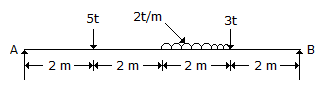
\includegraphics{../data_img/applied-mechanics-and-graphic-statics_1525414480-3.png}
}
\\\begin{enumerate*}[itemjoin=\qquad, label=\Alph*.]
\item{0.50}
\item{0.40}
\item{0.67}
\item{1.00}
\end{enumerate*}
\item{The reaction at the support B of the beam shown in below figure is \\

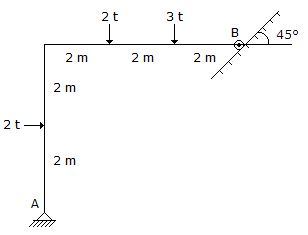
\includegraphics{../data_img/applied-mechanics-and-graphic-statics_1525414504-5.png}
}
\\\begin{enumerate*}[itemjoin=\qquad, label=\Alph*.]
\item{1.6 t}
\item{9.6 t}
\item{8.5 t}
\item{0.5 t}
\end{enumerate*}
\item{The reaction at the support D of the continuous beam ABCD, hinged at two points shown in below figure is \\

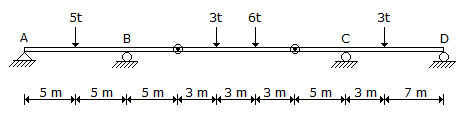
\includegraphics{../data_img/applied-mechanics-and-graphic-statics_1525414534-8.png}
}
\\\begin{enumerate*}[itemjoin=\qquad, label=\Alph*.]
\item{1.6 t ↑}
\item{1.6 t ↓}
\item{0.5 t ↑}
\item{0.5 t ↓}
\end{enumerate*}
\item{The reaction at the central support B of the beam ABC hinged at D shown in below figure is \\

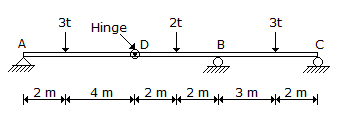
\includegraphics{../data_img/applied-mechanics-and-graphic-statics_1525414566-10.png}
}
\\\begin{enumerate*}[itemjoin=\qquad, label=\Alph*.]
\item{2 t}
\item{5.8 t}
\item{0.2 t}
\item{3.5 t}
\end{enumerate*}
\item{The reaction at the support `A' of the beam shown in below figure is \\

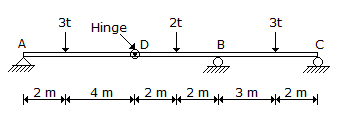
\includegraphics{../data_img/applied-mechanics-and-graphic-statics_1525414593-10.png}
}
\\\begin{enumerate*}[itemjoin=\qquad, label=\Alph*.]
\item{2 t}
\item{5.8 t}
\item{0.2 t}
\item{3.5 t}
\end{enumerate*}
\item{The load shared by the member BC of the structure shown in below figure is \\

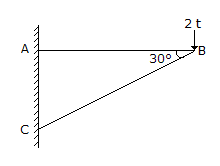
\includegraphics{../data_img/applied-mechanics-and-graphic-statics_1525414641-14.png}
}
\\\begin{enumerate*}[itemjoin=\qquad, label=\Alph*.]
\item{23 t}
\item{32 t}
\item{4 t}
\item{3 t}
\end{enumerate*}
\item{$ \omega $$ rad/sec is the angular velocity of a crank whose radius is r. If it makes $${\theta ^ \circ }$$ with inner dead centre and obliquity of the connecting rod $$l$$ is $$\varphi $$, the velocity v of the piston, is given by the equati $}
\\\begin{enumerate*}[itemjoin=\qquad, label=\Alph*.]
\item{$ {\omega ^2}\left( {l\cos \varphi + {\text{r}}\sin \varphi \tan \theta } \right) $}
\item{$ {\omega ^2}\left( {l\sin\varphi + {\text{r}}\cos \varphi \tan \theta } \right) $}
\item{$ \omega \left( {l\sin\varphi + {\text{r}}\cos \varphi \tan \theta } \right) $}
\item{$ {\omega ^2}\left( {l\sin\varphi - {\text{r}}\cos \theta \tan \varphi } \right) $}
\end{enumerate*}
\item{The unit of rotational inertia of a body in C.G.S system is}
\\\begin{enumerate*}[itemjoin=\qquad, label=\Alph*.]
\item{cm\^{}4}
\item{kg.cm\^{}2}
\item{gm.cm\^{}2}
\item{gm.cm\^{}3}
\end{enumerate*}
\item{A solid sphere of mass M and radius R rolls down a plane inclined at $$\theta $$ with the horizontal. The acceleration of sphere is (where g is acceleration due to gravity)}
\\\begin{enumerate*}[itemjoin=\qquad, label=\Alph*.]
\item{$ \frac{1}{3}{\text{g}}\sin \theta  $}
\item{$ \frac{2}{5}{\text{g}}\sin \theta  $}
\item{$ \frac{3}{7}{\text{g}}\sin \theta  $}
\item{$ \frac{5}{7}{\text{g}}\sin \theta  $}
\end{enumerate*}
\item{The ratio of unit of force in gravitational system to that in absolute system is (where `$${\text{g}}$$' is acceleration due to gravity)
}
\begin{enumerate}[label=\Alph*.]
\item{1}
\item{$ {\text{g}} $}
\item{$ \frac{1}{{\text{g}}} $}
\item{None of the above}
\end{enumerate}
\item{A heavy ladder resting on a floor and against a vertical wall may not be in equilibrium, if}
\begin{enumerate}[label=\Alph*.]
\item{Floor is smooth and the wall is rough}
\item{Floor is rough and the wall is smooth}
\item{Floor and wall both are smooth surfaces}
\item{Floor and wall both are rough surfaces}
\end{enumerate}
\item{A point subjected to a number of forces will be in equilibrium, if}
\begin{enumerate}[label=\Alph*.]
\item{Sum of resolved parts in any two directions at right angles, are both zero}
\item{Algebraic sum of the forces is zero}
\item{Two resolved parts in any two directions at right angles are equal}
\item{Algebraic sum of the moments of the forces about the point is zero}
\end{enumerate}
\item{If the tension in a cable supporting a lift moving upwards is twice the tension when the lift is moving downwards, the acceleration of the lift, is}
\\\begin{enumerate*}[itemjoin=\qquad, label=\Alph*.]
\item{$ \frac{{\text{g}}}{2} $}
\item{$ \frac{{\text{g}}}{3} $}
\item{$ \frac{{\text{g}}}{4} $}
\item{$ \frac{{\text{g}}}{5} $}
\end{enumerate*}
\item{Minimum potential energy of a system will be in the position of}
\begin{enumerate}[label=\Alph*.]
\item{Stable equilibrium}
\item{Unstable equilibrium}
\item{Neutral equilibrium}
\item{All of the above}
\end{enumerate}
\item{If the given forces P\_ 1, P\_ 2, P\_ 3 and P\_ 4 are such that the force polygon does not close, then the system will
}
\begin{enumerate}[label=\Alph*.]
\item{Be in equilibrium}
\item{Always reduce to a resultant force}
\item{Always reduce to a couple}
\item{Both (A) and (C)}
\end{enumerate}
\item{A shell travelling with a horizontal velocity of 100 m/sec explodes and splits into two parts, one of mass 10 kg and the other of 15 kg. The 15 kg mass drops vertically downward with initial velocity of 100 m/sec and the 10 kg mass begins to travel at an angle to the horizontal of tan\^{}-1x, where x is
}
\\\begin{enumerate*}[itemjoin=\qquad, label=\Alph*.]
\item{$ \frac{3}{4} $}
\item{$ \frac{4}{5} $}
\item{$ \frac{5}{3} $}
\item{$ \frac{3}{5} $}
\end{enumerate*}
\item{A ladder of weight 'w' rests against a smooth vertical wall and rests on rough horizontal ground, the coefficient of friction between the ladder and the ground being $$\frac{1}{4}$$. The maximum angle of inclination of the ladder to the vertical, if a man of weight 'w' is to walk to the top of it safely, is tan\^{}-1x, where x is}
\\\begin{enumerate*}[itemjoin=\qquad, label=\Alph*.]
\item{$ \frac{1}{4} $}
\item{$ \frac{1}{3} $}
\item{3}
\item{4}
\end{enumerate*}
\item{The length of a Second's pendulum, is}
\\\begin{enumerate*}[itemjoin=\qquad, label=\Alph*.]
\item{99.0 cm}
\item{99.4 cm}
\item{100 cm}
\item{101 cm}
\end{enumerate*}
\item{For a simple pendulum, the period of one oscillation is}
\\\begin{enumerate*}[itemjoin=\qquad, label=\Alph*.]
\item{$ 2\pi \sqrt {\frac{l}{{2{\text{g}}}}}  $}
\item{$ 2\pi \sqrt {\frac{{2{\text{g}}}}{l}}  $}
\item{$ 2\pi \sqrt {\frac{l}{{\text{g}}}}  $}
\item{$ 2\pi \sqrt {\frac{{\text{g}}}{{2l}}}  $}
\end{enumerate*}
\item{The locus of the instantaneous centre of a moving rigid body, is}
\\\begin{enumerate*}[itemjoin=\qquad, label=\Alph*.]
\item{Straight line}
\item{Involute}
\item{Centroid}
\item{Spiral}
\end{enumerate*}
\item{The inherent property of a body which offers reluctance to change its state of rest or uniform motion, is}
\\\begin{enumerate*}[itemjoin=\qquad, label=\Alph*.]
\item{Weight}
\item{Mass}
\item{Inertia}
\item{Momentum}
\end{enumerate*}
\item{Engineer's units of force, is}
\begin{enumerate}[label=\Alph*.]
\item{Newton in absolute units}
\item{Dyne in absolute units}
\item{Newton and dyne in absolute units}
\item{All the above}
\end{enumerate}
\item{If y is force and x is velocity, then dimensions of $$\frac{{{{\text{d}}^2}{\text{y}}}}{{{\text{d}}{{\text{x}}^2}}}$$ are}
\begin{enumerate}[label=\Alph*.]
\item{ML\^{}-1T\^{}-2}
\item{M\^{}2L\^{}-2T\^{}-2}
\item{ML\^{}-1T\^{}0}
\item{M\^{}2L\^{}-2T\^{}-4}
\end{enumerate}
\item{The moment of inertia of a hollow circular section whose external diameter is 8 cm and internal diameter is 6 cm, about centroidal axis, is}
\\\begin{enumerate*}[itemjoin=\qquad, label=\Alph*.]
\item{437.5 cm\^{}4}
\item{337.5 cm\^{}4}
\item{237.5 cm\^{}4}
\item{137.5 cm\^{}4}
\end{enumerate*}
\item{For a simple pendulum, time period for a beat, is}
\\\begin{enumerate*}[itemjoin=\qquad, label=\Alph*.]
\item{$ \pi \sqrt {\frac{l}{{\text{g}}}}  $}
\item{$ \pi \sqrt {\frac{{2l}}{{\text{g}}}}  $}
\item{$ \pi \sqrt {\frac{{\text{g}}}{{2l}}}  $}
\item{$ \pi \sqrt {\frac{l}{{2{\text{g}}}}}  $}
\item{$ \pi \sqrt {\frac{{2{\text{g}}}}{l}}  $}
\end{enumerate*}
\item{Free body diagram is an}
\begin{enumerate}[label=\Alph*.]
\item{Isolated joint with only body forces acting on it}
\item{Isolated joint with internal forces acting on it}
\item{Isolated joint with all the forces, internal as well as external, acting on it}
\item{None of the above}
\end{enumerate}
\item{Maximum efficiency of a screw jack for the angle of friction $$\theta $$, is
}
\\\begin{enumerate*}[itemjoin=\qquad, label=\Alph*.]
\item{$ \frac{{\sin \theta }}{{1 + \sin \theta }} $}
\item{$ \frac{{1 - \sin \theta }}{{\sin \theta }} $}
\item{$ \frac{{1 + \sin \theta }}{{1 - \sin \theta }} $}
\item{$ \frac{{1 - \sin \theta }}{{1 + \sin \theta }} $}
\end{enumerate*}
\item{For perfectly elastic bodies, the value of coefficient of restitution is}
\begin{enumerate}[label=\Alph*.]
\item{Zero}
\item{0.5}
\item{1.0}
\item{Between 0 and 1}
\end{enumerate}
\item{In a lifting machine with efficiency 60\%, an effort of 200 N is required to raise a load of 6 kN. The velocity ratio of the machine is}
\\\begin{enumerate*}[itemjoin=\qquad, label=\Alph*.]
\item{30}
\item{50}
\item{60}
\item{80}
\end{enumerate*}
\item{If a projectile is fired with an initial velocity of 10 m/sec at an angle of 60$^\circ$ to the horizontal, its horizontal and vertical velocity at the highest point of trajectory are
}
\begin{enumerate}[label=\Alph*.]
\item{0 and 5 m/sec}
\item{5 m/sec and 0}
\item{$ 5\sqrt 3 $$  m/sec and $}
\item{5 and $$5\sqrt 3 $$ ~m/sec}
\end{enumerate}
\item{The angle of projection for a range is equal to the distance through which the particle would have fallen in order to acquire a velocity equal to the velocity of projection, will be}
\\\begin{enumerate*}[itemjoin=\qquad, label=\Alph*.]
\item{30$^\circ$}
\item{45$^\circ$}
\item{60$^\circ$}
\item{75$^\circ$}
\end{enumerate*}
\item{An ordinate in a funicular polygon represents}
\begin{enumerate}[label=\Alph*.]
\item{Shear force}
\item{Resultant force}
\item{Bending moment}
\item{Equilibrium}
\end{enumerate}
\item{The Centre of gravity of a 10 $\times$ 15 $\times$ 5 cm T section from its bottom, is
}
\\\begin{enumerate*}[itemjoin=\qquad, label=\Alph*.]
\item{7.5 cm}
\item{5.0 cm}
\item{8.75 cm}
\item{7.85 cm}
\end{enumerate*}
\item{The piston of a steam engine moves with a simple harmonic motion. The crank rotates 120 r.p.m. and the stroke length is 2 meters. The linear velocity of the piston when it is at a distance of 0.5 metre from the centre, is}
\\\begin{enumerate*}[itemjoin=\qquad, label=\Alph*.]
\item{5.88 m/sec}
\item{8.88 m/sec}
\item{10.88 m/sec}
\item{12.88 m/sec}
\end{enumerate*}
\item{Pick up the correct statement from the following:}
\begin{enumerate}[label=\Alph*.]
\item{If two equal and perfectly elastic smooth spheres impinge directly, they interchange their velocities}
\item{If a sphere impinges directly on an equal sphere which is at rest, then a fraction $$\frac{1}{2}\left( {1 - {{\text{e}}^2}} \right)$$ ~ the original kinetic energy is lost by the impact}
\item{If a smooth sphere impinges on another sphere, which is at rest, the latter will move along the line of centres}
\item{If two equal spheres which are perfectly elastic impinge at right angles, their direction after impact will still be at right angles}
\item{All the above}
\end{enumerate}
\item{Pick up the correct statement from the following:}
\begin{enumerate}[label=\Alph*.]
\item{Nature plays an important role in the launch of a satellite}
\item{The earth's gravity reduces the speed of a satellite by 32 km per second}
\item{The gravitational force relents as the satellite climbs higher}
\item{All the above}
\end{enumerate}
\item{Pick up the incorrect statement from the following:}
\begin{enumerate}[label=\Alph*.]
\item{The C.G. of a circle is at its centre}
\item{The C.G. of a triangle is at the intersection of its medians}
\item{The C.G. of a rectangle is at the intersection of its diagonals}
\item{The C.G. of a semicircle is at a distance of r/2 from the centre}
\end{enumerate}
\item{The time period of a simple pendulum depends on \\
 (i) Mass of suspended particle \\
 (ii) Length of the pendulum \\
 (iii) Acceleration due to gravity}
\begin{enumerate}[label=\Alph*.]
\item{Only (i)}
\item{Both (ii) and (iii)}
\item{Both (i) and (iii)}
\item{All are correct}
\end{enumerate}
\item{The frequency of oscillation on moon as compared to that on earth, will be}
\begin{enumerate}[label=\Alph*.]
\item{2.44 times more}
\item{2.44 times less}
\item{3 times less}
\item{3 times more}
\end{enumerate}
\item{The direction of projection should bisect the angle between the inclined plane and the vertical for a range of a projectile on inclined plane}
\\\begin{enumerate*}[itemjoin=\qquad, label=\Alph*.]
\item{To be zero}
\item{To be maximum}
\item{To be minimum}
\item{None of these}
\end{enumerate*}
\item{The intrinsic equation of catenary is}
\begin{enumerate}[label=\Alph*.]
\item{S = c tan $\psi$}
\item{y = c cosh $$\frac{{\text{x}}}{{\text{c}}}$$}
\item{y = c cosh $\psi$}
\item{y = c sinh $\psi$}
\end{enumerate}
\item{Cartesian form of the equation of catenary is}
\begin{enumerate}[label=\Alph*.]
\item{y = c cosh $$\frac{{\text{x}}}{{\text{c}}}$$}
\item{y = c sinh $$\frac{{\text{x}}}{{\text{c}}}$$}
\item{y = c tan $$\frac{{\text{x}}}{{\text{c}}}$$}
\item{y = c sin $$\frac{{\text{x}}}{{\text{c}}}$$}
\end{enumerate}
\item{The instantaneous centre of a member lies at the point of intersection of two lines drawn at the ends of the member such that the lines are inclined to the direction of motion of the ends at}
\\\begin{enumerate*}[itemjoin=\qquad, label=\Alph*.]
\item{30$^\circ$}
\item{45$^\circ$}
\item{60$^\circ$}
\item{90$^\circ$}
\end{enumerate*}
\item{If two forces are in equilibrium, then the forces must \\
 (i) Be equal in magnitude \\
 (ii) Be opposite in sense \\
 (iii) Act along the same line}
\begin{enumerate}[label=\Alph*.]
\item{(i) and (ii)}
\item{(i) and (iii)}
\item{Only (i)}
\item{All (i), (ii) and (iii)}
\end{enumerate}
\item{The dimensions of power are}
\begin{enumerate}[label=\Alph*.]
\item{M\^{}2L\^{}2T\^{}-2}
\item{ML\^{}2T\^{}-3}
\item{M\^{}2LT\^{}-2}
\item{MLT\^{}-2}
\end{enumerate}
\item{The Law of Polygon of Forces states that}
\begin{enumerate}[label=\Alph*.]
\item{If a polygon representing the forces acting at point in a body is closed, the forces are in equilibrium}
\item{If forces acting on a point can be represented in magnitude and direction by the sides of a polygon taken in order, then the resultant of the forces will be represented in magnitude and direction by t}
\item{If forces acting on a point can be represented of a polygon taken in order, their sides of a polygon taken in order, their resultant will be represented in magnitude and direction by the closing side }
\item{If forces acting on a point can be represented in magnitude and direction by the sides of a polygon in order, the forces are in equilibrium}
\end{enumerate}
\item{A cube on a smooth horizontal surface}
\begin{enumerate}[label=\Alph*.]
\item{Cannot be in stable equilibrium}
\item{Cannot be in neutral equilibrium}
\item{Cannot be in unstable equilibrium}
\item{Can be in any of these states}
\end{enumerate}
\item{The mechanical advantage of an ideal machine is 100. For moving the local through 2 m, the effort moves through}
\\\begin{enumerate*}[itemjoin=\qquad, label=\Alph*.]
\item{0.02 m}
\item{2 m}
\item{2.5 m}
\item{20 m}
\end{enumerate*}
\item{The rate of change of displacement of a body with respect to its surrounding, is known}
\\\begin{enumerate*}[itemjoin=\qquad, label=\Alph*.]
\item{Velocity}
\item{Acceleration}
\item{Speed}
\item{None of these}
\end{enumerate*}
\item{A train weighing 196 tonnes experiences a frictional resistance of $$5\frac{{11}}{{22}}$$ ~per tonne. The speed of the train at the top of a down gradient 1 in 78.4 is 36 km/hour. The speed of the train after running 1 km down the slope, is}
\\\begin{enumerate*}[itemjoin=\qquad, label=\Alph*.]
\item{$ 5\sqrt {10} {\text{ m/sec}} $}
\item{$ 10\sqrt 5 {\text{ m/sec}} $}
\item{$ 5\sqrt 3 {\text{ m/sec}} $}
\item{$ 3\sqrt 5 {\text{ m/sec}} $}
\end{enumerate*}
\item{A trolley wire weighs 1 kg per metre length. The ends of the wire are attached to two poles 20 m apart. If the horizontal tension is 1000 kg, the central dip of the cable is}
\\\begin{enumerate*}[itemjoin=\qquad, label=\Alph*.]
\item{2 cm}
\item{3 cm}
\item{4 cm}
\item{5 cm}
\end{enumerate*}
\item{A particle moves along a straight line such that distance `x' traversed in `t' seconds is given by x = t\^{}2(t + 1), the acceleration of the particle, will be
}
\begin{enumerate}[label=\Alph*.]
\item{3t\^{}3 - 2t}
\item{3t\^{}2 + 2t}
\item{6t - 2}
\item{6t + 2}
\item{3t - 2}
\end{enumerate}
\item{A Seconds pendulum executes}
\begin{enumerate}[label=\Alph*.]
\item{0.5 beat per second}
\item{1.0 beat per second}
\item{2.0 beats per second}
\item{2.5 beats per second}
\end{enumerate}
\item{The forces which meet at one point and have their lines of action in different planes are called}
\begin{enumerate}[label=\Alph*.]
\item{Coplanar non-concurrent forces}
\item{Non-coplanar concurrent forces}
\item{Non-coplanar non-current forces}
\item{Intersecting forces}
\end{enumerate}
\end{enumerate}
\textbf{Answer Key}
\begin{tabular}{ | c | c c c c c c c c c c | }
\hline
 & 1 & 2 & 3 & 4 & 5 & 6 & 7 & 8 & 9 & 0 \\
\hline
0 & C & A & D & B & D & C & C & B & B & A \\
10 & D & B & B & C & B & B & D & C & B & B \\
20 & A & C & C & C & D & B & C & A & B & A \\
30 & B & D & B & B & C & C & C & A & B & D \\
40 & A & C & D & C & B & B & D & C & C & C \\
50 & E & D & D & B & B & B & A & A & D & D \\
60 & B & C & D & A & C & A & D & D & C & B \\
\hline
\end{tabular}
\clearpage
\subsection*{Section 5}
\begin{enumerate}
\item{The centre of gravity of a triangle is at the point where three}
\begin{enumerate}[label=\Alph*.]
\item{Medians of the triangle meet}
\item{Perpendicular bisectors of the sides of the triangle meet}
\item{Bisectors of the angle of the triangle meet}
\item{None of these}
\end{enumerate}
\item{If a flywheel increases its speed from 10 rpm to 20 rpm in 10 seconds, then its angular acceleration is}
\begin{enumerate}[label=\Alph*.]
\item{3.14 rad/sec 10}
\item{3.14 rad/sec 20}
\item{3.14 rad/sec 30}
\item{None of the above}
\end{enumerate}
\item{A ball of mass 250 g moving on a smooth horizontal table with a velocity of 10 m/sec hits an identical stationary ball `B' on the table. If the impact is perfectly plastic, the velocity of the ball `B' just after impact would be
}
\\\begin{enumerate*}[itemjoin=\qquad, label=\Alph*.]
\item{Zero}
\item{5 m/sec}
\item{10 m/sec}
\item{None of these}
\end{enumerate*}
\item{Ball `A' of mass 250 g moving on a smooth horizontal table with a velocity of 10 m/s hits an identical stationary ball `B' on the table. If the impact is perfectly elastic, the velocity of the ball `B' just after impact would be
}
\\\begin{enumerate*}[itemjoin=\qquad, label=\Alph*.]
\item{Zero}
\item{5 m/sec}
\item{10 m/sec}
\item{None of these}
\end{enumerate*}
\item{The diagram showing the point of application and line of action of forces in their plane is called}
\begin{enumerate}[label=\Alph*.]
\item{Vector diagram}
\item{Space diagram}
\item{Force diagram}
\item{Funicular diagram}
\end{enumerate}
\item{One end of a light string 4 m in length is fixed to a point on a smooth wall and the other end fastened to a point on the surface of a smooth sphere of diameter 2.25 m and of weight 100 kg. The reaction between the sphere and the wall of the arrangement made is}
\\\begin{enumerate*}[itemjoin=\qquad, label=\Alph*.]
\item{102.5 kg}
\item{105.5 kg}
\item{108.5 kg}
\item{110 kg}
\end{enumerate*}
\item{A rigid body suspended vertically at a point and oscillating with a small amplitude under the action of the force of gravity, is called}
\begin{enumerate}[label=\Alph*.]
\item{Simple pendulum}
\item{Compound pendulum}
\item{Second's pendulum}
\item{None of these}
\end{enumerate}
\item{When a body falls freely under gravitational force, it possesses}
\begin{enumerate}[label=\Alph*.]
\item{Maximum weight}
\item{Minimum weight}
\item{No weight}
\item{No effect on its weight}
\end{enumerate}
\item{Moment of inertia of a squares of side `b' about an axis through its centre of gravity, is
}
\\\begin{enumerate*}[itemjoin=\qquad, label=\Alph*.]
\item{$ \frac{{{{\text{b}}^3}}}{4} $}
\item{$ \frac{{{{\text{b}}^4}}}{{12}} $}
\item{$ \frac{{{{\text{b}}^4}}}{3} $}
\item{$ \frac{{{{\text{b}}^4}}}{8} $}
\end{enumerate*}
\item{When two forces, each equal to P, act at 90$^\circ$ to each other, then the resultant will be
}
\\\begin{enumerate*}[itemjoin=\qquad, label=\Alph*.]
\item{P}
\item{$ {\text{P}}\sqrt 2  $}
\item{$ \frac{{\text{P}}}{{\sqrt 2 }} $}
\item{2P}
\end{enumerate*}
\item{According to Law of Triangle of Forces}
\begin{enumerate}[label=\Alph*.]
\item{Three forces acting at a point, can be rep-resented by the sides of a triangle, each side being in proportion to the force}
\item{Three forces acting along the sides of a triangle are always in equilibrium}
\item{If three forces acting on a, point can be represented in magnitude and direction, by the sides of a triangle taken in order, these will be in equilibrium}
\item{If the forces acting on a particle be represented in magnitude and direction by the two sides of a triangle taken in order, their resultant will be represented in magnitude and direction by the third }
\end{enumerate}
\item{The dimensions of centrifugal force are}
\\\begin{enumerate*}[itemjoin=\qquad, label=\Alph*.]
\item{M1 L2 T2}
\item{M'L'T1}
\item{M'L'T2}
\item{M'L-`T2}
\end{enumerate*}
\item{Periodic time of body moving with simple harmonic motion, is}
\begin{enumerate}[label=\Alph*.]
\item{Directly proportional to its angular velocity}
\item{Directly proportional to the square of its angular velocity}
\item{Inversely proportional to the square of its angular velocity}
\item{Inversely proportional to its angular velocity}
\end{enumerate}
\item{The height at which the end of a rope of length $$l$$ should be tied so that a man pulling at the other end may have the greatest tendency to overturn the pillar, is
}
\\\begin{enumerate*}[itemjoin=\qquad, label=\Alph*.]
\item{$ \frac{3}{4}l $}
\item{$ \frac{1}{2}l $}
\item{$ \frac{l}{{\sqrt 2 }} $}
\item{$ \frac{2}{{\sqrt 3 }}l $}
\end{enumerate*}
\item{The ratio of the ranges on the inclined plane with motion upward and with motion downward for a given velocity, angle of projection will be}
\\\begin{enumerate*}[itemjoin=\qquad, label=\Alph*.]
\item{$ \frac{{\sin \left( {\alpha + \beta } \right)}}{{\sin \left( {\alpha - \beta } \right)}} $}
\item{$ \frac{{\sin \left( {\alpha - \beta } \right)}}{{\sin \left( {\alpha + \beta } \right)}} $}
\item{$ \frac{{\cos \left( {\alpha - \beta } \right)}}{{\cos \left( {\alpha + \beta } \right)}} $}
\item{$ \frac{{\tan \left( {\alpha - \beta } \right)}}{{\tan \left( {\alpha + \beta } \right)}} $}
\end{enumerate*}
\item{The C.G. of the shaded area of the bellow figure from the x-axis is \\

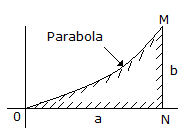
\includegraphics{../data_img/applied-mechanics-and-graphic-statics_1525414752-2.png}
}
\\\begin{enumerate*}[itemjoin=\qquad, label=\Alph*.]
\item{$ \frac{{\text{a}}}{4} $}
\item{$ \frac{{3{\text{a}}}}{4} $}
\item{$ \frac{{3{\text{b}}}}{{10}} $}
\item{$ \frac{{3{\text{a}}}}{{10}} $}
\item{$ \frac{{3{\text{a}}}}{5} $}
\end{enumerate*}
\item{The velocity of a body fallen from height `h', on reaching the ground is given by
}
\\\begin{enumerate*}[itemjoin=\qquad, label=\Alph*.]
\item{v = 2gh}
\item{v = 2gh\^{}2}
\item{$ {\text{v}} = \sqrt {2{\text{gh}}}  $}
\item{$ {\text{v}} = \frac{1}{{\sqrt {2{\text{gh}}} }} $}
\end{enumerate*}
\item{The C.G. of a right circular cone lies on its axis of symmetry at a height of}
\\\begin{enumerate*}[itemjoin=\qquad, label=\Alph*.]
\item{$ \frac{{\text{h}}}{2} $}
\item{$ \frac{{\text{h}}}{3} $}
\item{$ \frac{{\text{h}}}{4} $}
\item{$ \frac{{\text{h}}}{5} $}
\end{enumerate*}
\item{Centre of gravity of a thin hollow cone lies on the axis of symmetry at a height of}
\begin{enumerate}[label=\Alph*.]
\item{One-half of the total height above base}
\item{One-third of the total height above base}
\item{One-fourth of the total height above base}
\item{None of these}
\end{enumerate}
\item{The apparent weight of a man in a moving lift is less than his real weight when it is going down with}
\begin{enumerate}[label=\Alph*.]
\item{Uniform speed}
\item{An acceleration}
\item{Linear momentum}
\item{Retardation}
\end{enumerate}
\item{In simple harmonic motion, acceleration of a particle is proportional to}
\begin{enumerate}[label=\Alph*.]
\item{Rate of change of velocity}
\item{Displacement}
\item{Velocity}
\item{Direction}
\end{enumerate}
\item{The bending moment in an arch is proportional to}
\begin{enumerate}[label=\Alph*.]
\item{Vertical ordinate of funicular polygon}
\item{Vertical ordinate of the arch}
\item{Intercept between the arch axis and the funicular polygon}
\item{None of these}
\end{enumerate}
\item{The C.G. of a thin hollow cone of height `h', above its base lies on the axis, at a height of
}
\\\begin{enumerate*}[itemjoin=\qquad, label=\Alph*.]
\item{$ \frac{{\text{h}}}{3} $}
\item{$ \frac{{\text{h}}}{4} $}
\item{$ \frac{{2{\text{h}}}}{3} $}
\item{$ \frac{{3{\text{h}}}}{4} $}
\end{enumerate*}
\item{The maximum pull in a cable, carrying a uniformly distributed load and supported at two ends which are at the same level, is at}
\begin{enumerate}[label=\Alph*.]
\item{Supports}
\item{Quarter span}
\item{Mid span}
\item{None of the above}
\end{enumerate}
\item{The displacement of a particle which moves along a straight line is given by S = 4t\^{}3 + 3t\^{}2 - 10 where `S' is in meters and t is in seconds. The time taken by the particle to acquire a velocity of 18 m/sec from rest, is
}
\\\begin{enumerate*}[itemjoin=\qquad, label=\Alph*.]
\item{$ \frac{1}{2}$$ s $}
\item{1 sec}
\item{1.2 sec}
\item{1.5 sec}
\end{enumerate*}
\item{If the radius of the earth is 600 km the height of a mountain above sea level at the top of which a beat seconds pendulum at sea level, looses 27 seconds a day, is}
\\\begin{enumerate*}[itemjoin=\qquad, label=\Alph*.]
\item{500 meters}
\item{1000 meters}
\item{1500 meters}
\item{2000 meters}
\end{enumerate*}
\item{If a set of given forces are such that their free vectors build a closed polygon, then}
\begin{enumerate}[label=\Alph*.]
\item{The resultant force and resultant couple are always zero}
\item{The resultant force is zero but resultant couple is not zero}
\item{The resultant force is zero but resultant couple may not be zero}
\item{The resultant force and resultant couple both may not be zero}
\end{enumerate}
\item{The numbers of funicular polygons which can be drawn to pass through two specified points in the space diagram are}
\\\begin{enumerate*}[itemjoin=\qquad, label=\Alph*.]
\item{Zero}
\item{1}
\item{2}
\item{Infinity}
\end{enumerate*}
\item{The number of funicular polygons which can be drawn to pass through two specified points in the space diagram are}
\\\begin{enumerate*}[itemjoin=\qquad, label=\Alph*.]
\item{zero}
\item{1}
\item{2}
\item{infinity}
\end{enumerate*}
\item{Equation of motion of a point in a straight line, is}
\begin{enumerate}[label=\Alph*.]
\item{v = u + ft}
\item{S = ut + $$\frac{1}{2}$$ ft\^{}2}
\item{2fS = v\^{}2 - u\^{}2}
\item{All the above}
\end{enumerate}
\item{The tension in a cable supporting a lift}
\begin{enumerate}[label=\Alph*.]
\item{Is more when the lift is moving downwards}
\item{Is less when the lift is moving upwards}
\item{Remains constant whether its moves downwards or upwards}
\item{Is less when the lift is moving downwards}
\end{enumerate}
\item{Three forces which act on a rigid body to keep it in equilibrium. The forces must be coplanar and}
\begin{enumerate}[label=\Alph*.]
\item{Concurrent}
\item{Parallel}
\item{Concurrent parallel}
\item{None of these}
\end{enumerate}
\item{A stone is thrown up a slope of inclination 60$^\circ$ to the horizontal. At what angle to the slope must the stone be thrown so as to land as far as possible from the point of projection ?
}
\\\begin{enumerate*}[itemjoin=\qquad, label=\Alph*.]
\item{15$^\circ$}
\item{30$^\circ$}
\item{45$^\circ$}
\item{75$^\circ$}
\end{enumerate*}
\item{Two shots fired simultaneously from the top and bottom of a vertical tower with elevations of 30$^\circ$ and 45$^\circ$ respectively strike a target simultaneously. If horizontal distance of the target from the tower is 1000 m, the height of the tower is
}
\\\begin{enumerate*}[itemjoin=\qquad, label=\Alph*.]
\item{350 m}
\item{375 m}
\item{400 m}
\item{425 m}
\end{enumerate*}
\item{A body of weight 14 g appears to weight 13 g when weighed by a spring balance in a moving lift. The acceleration of the lift at that moment was}
\\\begin{enumerate*}[itemjoin=\qquad, label=\Alph*.]
\item{0.5 m/sec\^{}2}
\item{0.7 m/sec\^{}2}
\item{1 m/sec\^{}2}
\item{1 cm/sec\^{}2}
\end{enumerate*}
\item{A Second's pendulum gains 2 minutes a day. To make it to keep correct time its length}
\begin{enumerate}[label=\Alph*.]
\item{Must be decreased}
\item{Must be increased}
\item{Is not changed but weight of the bob is increased}
\item{Is not changed but weight of the bob is decreased}
\end{enumerate}
\item{The centre of gravity of a homogeneous body is the point at which the whole}
\begin{enumerate}[label=\Alph*.]
\item{Volume of the body is assumed to be concentrated}
\item{Area of the surface of the body is assumed to be concentrated}
\item{Weight of the body is assumed to be concentrated}
\item{All the above}
\end{enumerate}
\item{The following is in unstable equilibrium}
\begin{enumerate}[label=\Alph*.]
\item{A uniform solid cone resting on a generator on a smooth horizontal plane}
\item{A uniform solid cone resting on its base on a horizontal plane}
\item{A solid cube resting on one edge}
\item{A satellite encircling the earth}
\end{enumerate}
\item{Time required to stop a car moving with a velocity 20 m/sec within a distance of 40 m, is}
\\\begin{enumerate*}[itemjoin=\qquad, label=\Alph*.]
\item{2 sec}
\item{3 sec}
\item{4 sec}
\item{5 sec}
\end{enumerate*}
\item{A uniform rod 9 m long weighing 40 kg is pivoted at a point 2 m from one end where a weight of 120 kg is suspended. The required force acting at the end in a direction perpendicular to rod to keep it equilibrium, at an inclination 60$^\circ$ with horizontal, is
}
\\\begin{enumerate*}[itemjoin=\qquad, label=\Alph*.]
\item{40 kg}
\item{60 kg}
\item{10 kg}
\item{100 kg}
\end{enumerate*}
\item{A sphere and a cylinder having the same mass and radii start from rest and roll down the same inclined plane. Which body gets to the bottom first?}
\begin{enumerate}[label=\Alph*.]
\item{Sphere with greater rotational energy at bottom than cylinder}
\item{Sphere with lesser rotational energy at bottom than cylinder}
\item{Cylinder with greater rotational energy at bottom than sphere}
\item{Both reach the bottom simultaneously with equal rotational energy at bottom}
\end{enumerate}
\item{A light rope is loaded with many equal weights at equal horizontal intervals. The points of suspension on the rope lie on a}
\\\begin{enumerate*}[itemjoin=\qquad, label=\Alph*.]
\item{Parabola}
\item{Catenary}
\item{Cycloid}
\item{Ellipse}
\end{enumerate*}
\item{If the resultant of two forces has the same magnitude as either of the force, then the angle between the two forces is}
\\\begin{enumerate*}[itemjoin=\qquad, label=\Alph*.]
\item{30$^\circ$}
\item{45$^\circ$}
\item{60$^\circ$}
\item{120$^\circ$}
\end{enumerate*}
\item{If the resultant of two forces P and Q acting at an angle $$\theta $$ makes an angle $$\alpha $$ with P, then tan $$\alpha $$ equals
}
\\\begin{enumerate*}[itemjoin=\qquad, label=\Alph*.]
\item{$ \frac{{{\text{P}}\sin \theta }}{{{\text{P}} - {\text{Q}}\cos \theta }} $}
\item{$ \frac{{{\text{Q}}\sin \theta }}{{{\text{P}} + {\text{Q}}\cos \theta }} $}
\item{$ \frac{{{\text{P}}\sin \theta }}{{{\text{P}} + {\text{Q}}\tan\theta }} $}
\item{$ \frac{{{\text{Q}}\sin \theta }}{{{\text{P}} + {\text{Q}}\sin\theta }} $}
\end{enumerate*}
\item{The motion of a particle moving with S.H.M. from an extremity to the other, constitutes}
\begin{enumerate}[label=\Alph*.]
\item{Half an oscillation}
\item{One full oscillation}
\item{Two oscillations}
\item{None of these}
\end{enumerate}
\item{The unit of Moment of Inertia of a body, is}
\\\begin{enumerate*}[itemjoin=\qquad, label=\Alph*.]
\item{m}
\item{m\^{}2}
\item{m\^{}3}
\item{m\^{}4}
\end{enumerate*}
\item{The angle of projection at which the horizontal range and maximum height of a projectile are equal to}
\\\begin{enumerate*}[itemjoin=\qquad, label=\Alph*.]
\item{36$^\circ$}
\item{45$^\circ$}
\item{56$^\circ$}
\item{76$^\circ$}
\end{enumerate*}
\item{The angle of projection at which the horizontal range and maximum height of a projectile are equal to}
\\\begin{enumerate*}[itemjoin=\qquad, label=\Alph*.]
\item{45}
\item{$ \theta = {\tan ^{ - 1}}\left( {0.25} \right) $}
\item{$ \theta = {\tan ^{ - 1}}4{\text{ or }}\theta = 70 $}
\item{60}
\end{enumerate*}
\item{A rigid body is in a stable equilibrium if the application of any force}
\begin{enumerate}[label=\Alph*.]
\item{Can raise the CG of the body but cannot lower it}
\item{Tends to lower the CG of the body}
\item{Neither raises nor lowers the CG of the body}
\item{None of above}
\end{enumerate}
\item{What is the answer to this question? \\
 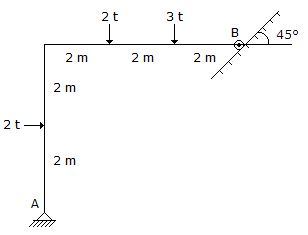
\includegraphics{../data_img/applied-mechanics-and-graphic-statics_1525414812-5.png}
}
\\\begin{enumerate*}[itemjoin=\qquad, label=\Alph*.]
\item{10.8 t}
\item{10.6 t}
\item{10.4 t}
\item{10.2 t}
\end{enumerate*}
\item{What is the answer to this question? \\

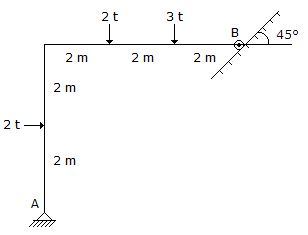
\includegraphics{../data_img/applied-mechanics-and-graphic-statics_1525414834-5.png}
}
\\\begin{enumerate*}[itemjoin=\qquad, label=\Alph*.]
\item{Zero}
\item{2 t}
\item{3 t}
\item{1 t}
\end{enumerate*}
\item{Which of the following represents the state of neutral equilibrium?}
\begin{enumerate}[label=\Alph*.]
\item{A cube resting on one edge}
\item{A smooth cylinder lying on a curved surface}
\item{A smooth cylinder lying on a convex surface}
\item{None of the above}
\end{enumerate}
\item{A square hole is made in a circular lamina, the diagonal of the square is equal to the radius of the circle as shown in below figure the shift in the centre of gravity is \\

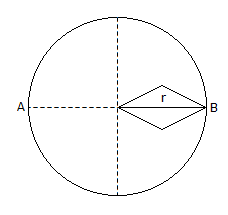
\includegraphics{../data_img/applied-mechanics-and-graphic-statics_1525414864-6.png}
}
\\\begin{enumerate*}[itemjoin=\qquad, label=\Alph*.]
\item{$ \frac{{{\text{r}}\left( {\pi - 0.75} \right)}}{{\left( {\pi - 0.5} \right)}} $}
\item{$ \frac{{{\text{r}}\left( {\pi - 0.25} \right)}}{{\left( {\pi - 0.75} \right)}} $}
\item{$ \frac{{{\text{r}}\left( {\pi - 0.5} \right)}}{{\left( {\pi - 0.75} \right)}} $}
\item{$ \frac{{{\text{r}}\left( {\pi - 0.5} \right)}}{{\left( {\pi - 0.25} \right)}} $}
\end{enumerate*}
\item{The potential energy of a particle falling through a straight shaft drilled through the earth (assumed homogenous and spherical) is proportional to (where r is the distance of'the particle from centre of the earth)}
\\\begin{enumerate*}[itemjoin=\qquad, label=\Alph*.]
\item{log r}
\item{r}
\item{r\^{}2}
\item{$ \frac{1}{{\text{r}}} $}
\end{enumerate*}
\item{A stone is whirled in a vertical circle, the tension in the string, is maximum}
\begin{enumerate}[label=\Alph*.]
\item{When the string is horizontal}
\item{When the stone is at the highest position}
\item{When the stone is at the lowest position}
\item{At all the positions}
\end{enumerate}
\item{The graphical method of determining the forces in the members of a truss is based on}
\begin{enumerate}[label=\Alph*.]
\item{Method of joint}
\item{Method of section}
\item{Either method}
\item{None of the two methods}
\end{enumerate}
\item{The shape of a suspended cable under its own weight, is}
\\\begin{enumerate*}[itemjoin=\qquad, label=\Alph*.]
\item{Parabolic}
\item{Circular}
\item{Catenary}
\item{Elliptical}
\end{enumerate*}
\item{The maximum value of the horizontal range for a projectile projected with a velocity of 98 m/sec is}
\\\begin{enumerate*}[itemjoin=\qquad, label=\Alph*.]
\item{98 m}
\item{490 m}
\item{980 m}
\item{1960 m}
\end{enumerate*}
\item{A geo-stationary satellite is one which orbits the earth with a velocity of rotation of}
\\\begin{enumerate*}[itemjoin=\qquad, label=\Alph*.]
\item{Moon}
\item{Earth}
\item{Sun}
\item{Pole}
\end{enumerate*}
\item{A particle moving with a simple harmonic motion, attains its maximum velocity when it passes}
\begin{enumerate}[label=\Alph*.]
\item{The extreme point of the oscillation}
\item{Through the mean position}
\item{Through a point at half amplitude}
\item{None of these}
\end{enumerate}
\item{A square hole is punched out of a circular lamina, the diagonal of the square being the radius of the circle. If `r' is the radius of the circle, the C.G. of the remainder from the corner of the square on the circumference will be
}
\\\begin{enumerate*}[itemjoin=\qquad, label=\Alph*.]
\item{$ \frac{{{\text{r}}\left( {\pi + 0.25} \right)}}{{\pi - 0.5}} $}
\item{$ \frac{{{\text{r}}\left( {\pi - 0.5} \right)}}{{\pi + 0.25}} $}
\item{$ \frac{{{\text{r}}\left( {\pi - 0.25} \right)}}{{\pi - 0.5}} $}
\item{$ \frac{{{\text{r}}\left( {\pi + 0.25} \right)}}{{\pi + 0.5}} $}
\end{enumerate*}
\item{The practical units of work, is}
\\\begin{enumerate*}[itemjoin=\qquad, label=\Alph*.]
\item{Erg}
\item{Joule}
\item{Newton}
\item{Dyne}
\end{enumerate*}
\item{According to Kennedy's theorem, if three bodies have plane motions, their instantaneous centers lie on}
\begin{enumerate}[label=\Alph*.]
\item{A point}
\item{A straight line}
\item{Two straight lines}
\item{A triangle}
\end{enumerate}
\item{The moment of inertia of the shaded portion of the area shown in below figure about the X-axis, is \\

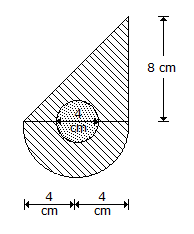
\includegraphics{../data_img/applied-mechanics-and-graphic-statics_1525414908-15.png}
}
\\\begin{enumerate*}[itemjoin=\qquad, label=\Alph*.]
\item{229.34 cm\^{}4}
\item{329.34 cm\^{}4}
\item{429.34 cm\^{}4}
\item{529.34 cm\^{}4}
\end{enumerate*}
\item{Two forces of 6 Newtons and 8 Newtons which are acting at right angles to each other, will have a resultant of}
\\\begin{enumerate*}[itemjoin=\qquad, label=\Alph*.]
\item{5 Newtons}
\item{8 Newtons}
\item{10 Newtons}
\item{12 Newtons}
\end{enumerate*}
\item{A satellite is said to move in a synchronous orbit if it moves at an altitude of 36,000 km with a maximum velocity of about}
\begin{enumerate}[label=\Alph*.]
\item{7000 km per hour}
\item{8000 km per hour}
\item{9000 km per hour}
\item{11,000 km per hour}
\end{enumerate}
\item{Two balls of masses 3 kg and 6 kg are moving with velocities of 4 m/sec and 1 m/sec respectively, towards each other along the line of their centers. After impact the 3 kg ball comes to rest. This can happen only if the coefficient of restitution between the balls is}
\\\begin{enumerate*}[itemjoin=\qquad, label=\Alph*.]
\item{$ \frac{2}{3} $}
\item{$ \frac{1}{5} $}
\item{$ \frac{3}{5} $}
\item{$ \frac{1}{3} $}
\end{enumerate*}
\item{The velocity ratio of the differential wheel and axle is}
\\\begin{enumerate*}[itemjoin=\qquad, label=\Alph*.]
\item{$ \frac{{\text{R}}}{{{{\text{r}}_1} - {{\text{r}}_2}}} $}
\item{$ \frac{{2{\text{R}}}}{{{{\text{r}}_1}}} $}
\item{$ \frac{{3{\text{R}}}}{{{{\text{r}}_1} - {{\text{r}}_2}}} $}
\item{$ \frac{{2{\text{R}}}}{{{{\text{r}}_1} + {{\text{r}}_2}}} $}
\end{enumerate*}
\item{A solid cylinder of mass M and radius R rolls down an inclined plane without slipping. The acceleration of center of mass of rolling cylinder is (where `$${\text{g}}$$' is acceleration due to gravity and $$\theta $$ is inclination of plane with horizontal.)
}
\\\begin{enumerate*}[itemjoin=\qquad, label=\Alph*.]
\item{$ \frac{1}{3}{\text{g}}\sin \theta  $}
\item{$ \frac{2}{3}{\text{g}}\cos \theta  $}
\item{$ \frac{2}{3}{\text{g}}\sin \theta  $}
\item{$ {\text{g}}\sin \theta  $}
\end{enumerate*}
\item{A body is dropped from a height of 100 m and at the same time another body is projected vertically upward with a velocity of 10 m/sec. The two particles will}
\begin{enumerate}[label=\Alph*.]
\item{Never meet}
\item{Meet after 1 sec}
\item{Meet after 5 sec}
\item{Meet after 10 sec}
\end{enumerate}
\end{enumerate}
\textbf{Answer Key}
\begin{tabular}{ | c | c c c c c c c c c c | }
\hline
 & 1 & 2 & 3 & 4 & 5 & 6 & 7 & 8 & 9 & 0 \\
\hline
0 & A & C & A & C & B & A & B & C & B & B \\
10 & D & C & D & C & B & C & C & C & B & B \\
20 & B & C & C & A & B & D & C & D & D & D \\
30 & D & A & A & D & B & B & C & C & C & C \\
40 & B & A & D & B & A & D & D & C & A & A \\
50 & A & D & A & C & C & A & C & C & B & B \\
60 & C & B & B & C & C & D & B & B & C & D \\
\hline
\end{tabular}
\clearpage
\subsection*{Section 6}
\begin{enumerate}
\item{A smooth cylinder lying on its convex surface remains}
\begin{enumerate}[label=\Alph*.]
\item{In stable equilibrium}
\item{In unstable equilibrium}
\item{In neutral equilibrium}
\item{Out of equilibrium}
\end{enumerate}
\item{A projectile is fired at an angle `$\theta$' to the vertical. Its horizontal range will be maximum when `$\theta$' is
}
\\\begin{enumerate*}[itemjoin=\qquad, label=\Alph*.]
\item{0$^\circ$}
\item{30$^\circ$}
\item{45$^\circ$}
\item{90$^\circ$}
\end{enumerate*}
\item{The total kinetic energy of a hoop of mass 2 kg and radius 4 m sliding with linear velocity 8 m/sec and angular velocity 5 radian/sec is}
\\\begin{enumerate*}[itemjoin=\qquad, label=\Alph*.]
\item{64 J}
\item{400 J}
\item{464 J}
\item{89 J}
\end{enumerate*}
\item{Angular acceleration of a particle may be expressed as}
\begin{enumerate}[label=\Alph*.]
\item{Radians/sec\^{}2}
\item{Degrees/sec\^{}2}
\item{Revolutions/sec}
\item{All the above}
\end{enumerate}
\item{A symmetrical body is rotating about its axis of symmetry, its moment of inertia about the axis of rotation being 1 kg-m\^{}2 and its rate of rotation 2 rev/sec. The angular momentum of the body in kg-m\^{}2/sec is}
\\\begin{enumerate*}[itemjoin=\qquad, label=\Alph*.]
\item{1.257 }
\item{12.57}
\item{13.57}
\item{1.357}
\end{enumerate*}
\end{enumerate}
\textbf{Answer Key}
\begin{tabular}{ | c | c c c c c c c c c c | }
\hline
 & 1 & 2 & 3 & 4 & 5 & 6 & 7 & 8 & 9 & 0 \\
\hline
0 & B & C & C & D & C &   &   &   &   &   \\
\hline
\end{tabular}
\clearpage
\section{Environmental Engineering}
\subsection*{Section 1}
\begin{enumerate}
\item{Which of the following values of pH represents a stronger acid?}
\\\begin{enumerate*}[itemjoin=\qquad, label=\Alph*.]
\item{2}
\item{5}
\item{7}
\item{10}
\end{enumerate*}
\item{The distribution mains are designed for}
\begin{enumerate}[label=\Alph*.]
\item{Maximum daily demand}
\item{Maximum hourly demand}
\item{Average daily demand}
\item{Maximum hourly demand on maximum day}
\end{enumerate}
\item{Sewage treatment units are designed for}
\begin{enumerate}[label=\Alph*.]
\item{Maximum flow only}
\item{Minimum flow only}
\item{Average flow only}
\item{Maximum and minimum flow}
\end{enumerate}
\item{For satisfactory working of a sludge digestion unit, the pH range of digested sludge should be maintained as}
\\\begin{enumerate*}[itemjoin=\qquad, label=\Alph*.]
\item{4.5 to 6.0}
\item{6.5 to 8.0}
\item{8.5 to 10.0}
\item{10.5 to 12.0}
\end{enumerate*}
\item{The pathogens can be killed by}
\begin{enumerate}[label=\Alph*.]
\item{Nitrification}
\item{Chlorination}
\item{Oxidation}
\item{None of the above}
\end{enumerate}
\item{Orthotolidine test is used for determination of}
\begin{enumerate}[label=\Alph*.]
\item{Dissolved oxygen}
\item{Residual chlorine}
\item{Biochemical oxygen demand}
\item{Dose of coagulant}
\end{enumerate}
\item{Period of cleaning of slow sand filters is about}
\\\begin{enumerate*}[itemjoin=\qquad, label=\Alph*.]
\item{24 - 48 hours}
\item{10 - 12 days}
\item{2 - 3 months}
\item{1 - 2 year}
\end{enumerate*}
\item{The rate of filtration in slow sand filters in million litres per day per hectare is about}
\\\begin{enumerate*}[itemjoin=\qquad, label=\Alph*.]
\item{50 to 60}
\item{100 to 150}
\item{500 to 600}
\item{1400 to 1500}
\end{enumerate*}
\item{The working conditions in imhoff tanks are}
\begin{enumerate}[label=\Alph*.]
\item{Aerobic only}
\item{Anaerobic only}
\item{Aerobic in lower compartment and anaerobic in upper compartment}
\item{Anaerobic in lower compartment and aerobic in upper compartment}
\end{enumerate}
\item{The self cleansing velocity for all sewers in India is usually}
\begin{enumerate}[label=\Alph*.]
\item{Less than 1.0 m/sec}
\item{1.0 m/sec to 1.2 m/sec}
\item{1.5 m/sec to 2.0 m/sec}
\item{3.0 m/sec to 3.5 m/sec}
\end{enumerate}
\item{The method of analysis of distribution system in which the domestic supply is neglected and fire demand is considered is}
\begin{enumerate}[label=\Alph*.]
\item{Circle method}
\item{Equivalent pipe method}
\item{Electrical analysis method}
\item{Hardy cross method}
\end{enumerate}
\item{Residual chlorine in water is determined by}
\begin{enumerate}[label=\Alph*.]
\item{Starch iodide method}
\item{Orthotolidine method}
\item{Both (A) and (B)}
\item{None of the above}
\end{enumerate}
\item{The means of access for inspection and cleaning of sewer line is known as}
\\\begin{enumerate*}[itemjoin=\qquad, label=\Alph*.]
\item{Inlet}
\item{Manhole}
\item{Drop manhole}
\item{Catch basin}
\end{enumerate*}
\item{The phenolic compounds in public water supply should not be more than}
\\\begin{enumerate*}[itemjoin=\qquad, label=\Alph*.]
\item{0.1 ppm}
\item{0.01 ppm}
\item{0.001 ppm}
\item{0.0001 ppm}
\end{enumerate*}
\item{The water carriage system of collection of waste product}
\begin{enumerate}[label=\Alph*.]
\item{Is cheaper in initial cost than dry conservancy system}
\item{Requires treatment before disposal}
\item{Creates hygienic problem}
\item{All of the above}
\end{enumerate}
\item{In chlorination, with the rise in temperature of water, death rate of bacteria}
\begin{enumerate}[label=\Alph*.]
\item{Increases}
\item{Decreases}
\item{Remains unaffected}
\item{None of the above}
\end{enumerate}
\item{The characteristics of fresh and septic sewage respectively are}
\begin{enumerate}[label=\Alph*.]
\item{Acidic and alkaline}
\item{Alkaline and acidic}
\item{Both acidic}
\item{Both alkaline}
\end{enumerate}
\item{An egg shaped section of sewer}
\begin{enumerate}[label=\Alph*.]
\item{Is economical than circular section}
\item{Provides self cleansing velocity at low discharges}
\item{Is more stable than circular section}
\item{Is easy to construct}
\end{enumerate}
\item{Most suitable section of sewer in separate sewage system is}
\begin{enumerate}[label=\Alph*.]
\item{Rectangular section}
\item{Circular section}
\item{Standard form of egg shaped sewer}
\item{Modified egg shaped section}
\end{enumerate}
\item{A sewer that receives the discharge of a number of house sewers is called}
\begin{enumerate}[label=\Alph*.]
\item{House sewer}
\item{Lateral sewer}
\item{Intercepting sewer}
\item{Sub-main sewer}
\end{enumerate}
\item{Standard EDTA (ethylene diamine tetra acetic acid) solution is used to determine the}
\begin{enumerate}[label=\Alph*.]
\item{Hardness in water}
\item{Turbidity in water}
\item{Dissolved oxygen in water}
\item{Residual chlorine in water}
\end{enumerate}
\item{The hourly variation factor is usually taken as}
\\\begin{enumerate*}[itemjoin=\qquad, label=\Alph*.]
\item{1.5}
\item{1.8}
\item{2.0}
\item{2.7}
\end{enumerate*}
\item{Disinfection of water results in}
\begin{enumerate}[label=\Alph*.]
\item{Removal of turbidity}
\item{Removal of hardness}
\item{Killing of disease bacteria}
\item{Complete sterilisation}
\end{enumerate}
\item{If the total hardness of water is greater than its total alkalinity, the carbonate hardness will be equal to}
\begin{enumerate}[label=\Alph*.]
\item{Total alkalinity}
\item{Total hardness}
\item{Total hardness total alkalinity}
\item{Non carbonate hardness}
\end{enumerate}
\item{Laying of sewers is usually done with the help of}
\begin{enumerate}[label=\Alph*.]
\item{A Theodolite}
\item{A compass}
\item{Sight rails and boning rods}
\item{A plane table}
\end{enumerate}
\item{The correct relation between theoretical oxygen demand (TOD), Biochemical oxygen demand (BOD) and Chemical oxygen demand (COD) is given by}
\begin{enumerate}[label=\Alph*.]
\item{TOD > BOD > COD}
\item{TOD > COD > BOD}
\item{BOD > COD > TOD}
\item{COD > BOD > TOD}
\end{enumerate}
\item{As compared to shallow wells, deep wells have}
\\\begin{enumerate*}[itemjoin=\qquad, label=\Alph*.]
\item{More depth}
\item{Less depth}
\item{More discharge}
\item{Less discharge}
\end{enumerate*}
\item{As compared to cast iron pipes, steel pipes are}
\begin{enumerate}[label=\Alph*.]
\item{Heavier}
\item{Stronger}
\item{Costlier}
\item{Less susceptible to corrosion}
\end{enumerate}
\item{In water treatment, rapid gravity filters are adopted to remove}
\begin{enumerate}[label=\Alph*.]
\item{Dissolved organic substances}
\item{Dissolved solids and dissolved gases}
\item{Floating solids and dissolved inorganic solids}
\item{Bacteria and colloidal solids}
\end{enumerate}
\item{In facultative stabilization pond, the sewage is treated by}
\begin{enumerate}[label=\Alph*.]
\item{Aerobic bacteria only}
\item{Algae only}
\item{Dual action of aerobic bacteria and anaerobic bacteria}
\item{Sedimentation}
\end{enumerate}
\item{The gas from sludge digestion tank is mainly composed of}
\begin{enumerate}[label=\Alph*.]
\item{Nitrogen}
\item{Carbon dioxide}
\item{Hydrogen sulphide}
\item{Methane}
\end{enumerate}
\item{The maximum efficiency of BOD removal is achieved in}
\begin{enumerate}[label=\Alph*.]
\item{Oxidation pond}
\item{Oxidation ditch}
\item{Aerated lagoons}
\item{Trickling filters}
\end{enumerate}
\item{The minimum and maximum diameters of sewers shall preferably be}
\begin{enumerate}[label=\Alph*.]
\item{15 cm and 100 cm}
\item{15 cm and 300 cm}
\item{30 cm and 450 cm}
\item{60 cm and 300 cm}
\end{enumerate}
\item{The biochemical treatment of sewage effluents is essentially a process of}
\\\begin{enumerate*}[itemjoin=\qquad, label=\Alph*.]
\item{Oxidation}
\item{Dehydration}
\item{Reduction}
\item{Alkalinization}
\end{enumerate*}
\item{Sewerage system is usually designed for}
\\\begin{enumerate*}[itemjoin=\qquad, label=\Alph*.]
\item{10 years}
\item{25 years}
\item{50 years}
\item{75 years}
\end{enumerate*}
\item{Sewage treatment units are normally designed for}
\\\begin{enumerate*}[itemjoin=\qquad, label=\Alph*.]
\item{5 - 10 years}
\item{15 - 20 years}
\item{30 - 40 years}
\item{40 - 50 years}
\end{enumerate*}
\item{Generally the detention period for grit chambers is kept as}
\\\begin{enumerate*}[itemjoin=\qquad, label=\Alph*.]
\item{1 minute}
\item{5 minutes}
\item{24 hours}
\item{12 hours}
\end{enumerate*}
\item{Activated carbon is used for}
\begin{enumerate}[label=\Alph*.]
\item{Disinfection}
\item{Removing hardness}
\item{Removing odours}
\item{Removing corrosiveness}
\end{enumerate}
\item{The polluted water is one which}
\begin{enumerate}[label=\Alph*.]
\item{Contains pathogenic bacteria}
\item{Consists of undesirable substances rendering it unfit for drinking and domestic use}
\item{Is safe and suitable for drinking and domestic use}
\item{Is contaminated}
\end{enumerate}
\item{In a BOD test, 1.0 ml of raw sewage was diluted to 100 ml and the dissolved oxygen concentration of diluted sample at the beginning was 6 ppm and it was 4 ppm at the end of 5 day incubation at 20$^\circ$C. The BOD of raw sewage will be
}
\\\begin{enumerate*}[itemjoin=\qquad, label=\Alph*.]
\item{100 ppm}
\item{200 ppm}
\item{300 ppm}
\item{400 ppm}
\end{enumerate*}
\item{The amount of residual chlorine left in public water supply for safety against pathogenic bacteria is about}
\begin{enumerate}[label=\Alph*.]
\item{0.01 to 0.05 ppm}
\item{0.05 to 0.5 ppm}
\item{0.5 to 1.0 ppm}
\item{1.0 to 5.0 ppm}
\end{enumerate}
\item{Which of the following retards the self purification of stream?}
\begin{enumerate}[label=\Alph*.]
\item{Higher temperature}
\item{Sunlight}
\item{Satisfying oxygen demand}
\item{None of the above}
\end{enumerate}
\item{As compared to rapid sand filters, slow sand filters give \\
 (i) Slower filtration rate \\
 (ii) Higher filtration rate \\
 (iii) Lesser efficiency in removal of bacteria \\
 (iv) Higher efficiency in removal of bacteria \\
 The correct answer is}
\\\begin{enumerate*}[itemjoin=\qquad, label=\Alph*.]
\item{(i) and (ii)}
\item{(ii) and (iii)}
\item{(i) and (iv)}
\item{(ii) and (iv)}
\end{enumerate*}
\item{The amount of coagulant needed for coagulation of water increases with \\

(i) Increase in turbidity of water \\

(ii) Decrease in turbidity of water \\

(iii) Increase in temperature of water \\

(iv) Decrease in temperature of water \\

The correct answer is}
\\\begin{enumerate*}[itemjoin=\qquad, label=\Alph*.]
\item{(i) and (ii)}
\item{(i) and (iv)}
\item{(ii) and (iii)}
\item{(ii) and (iv)}
\end{enumerate*}
\item{Cleaning is done by \\
 (i) Scraping and removal in filters slow sand \\
 (ii) Back washing in slow sand filters \\
 (iii) Scraping and removal in filters rapid sand \\
 (iv) Back washing in rapid sand filters \\
The correct answer is}
\\\begin{enumerate*}[itemjoin=\qquad, label=\Alph*.]
\item{(i) and (ii)}
\item{(ii) and (iii)}
\item{(i) and (iv)}
\item{(ii) and (iv)}
\end{enumerate*}
\item{Sludge volume index is defined as the ratio of}
\begin{enumerate}[label=\Alph*.]
\item{Percentage of sludge by volume to percentage of suspended solids by weight}
\item{Percentage of sludge by volume to percentage of total solids by weight}
\item{Percentage of suspended solids by weight to percentage of sludge by volume}
\item{Percentage of total solids by weight to percentage of sludge by volume}
\end{enumerate}
\item{The maximum permissible limit for fluoride in drinking water is}
\\\begin{enumerate*}[itemjoin=\qquad, label=\Alph*.]
\item{0.1 mg/liter}
\item{1.5 mg/liter}
\item{5 mg/liter}
\item{10 mg/liter}
\end{enumerate*}
\item{Facultative bacteria are able to work in}
\begin{enumerate}[label=\Alph*.]
\item{Presence of oxygen only}
\item{Absence of oxygen only}
\item{Presence as well as in absence of oxygen}
\item{Presence of water}
\end{enumerate}
\item{The minimum dissolved oxygen which should always be present in water in order to save the aquatic life is}
\\\begin{enumerate*}[itemjoin=\qquad, label=\Alph*.]
\item{1 ppm}
\item{4 ppm}
\item{10 ppm}
\item{40 ppm}
\end{enumerate*}
\item{The dissolved oxygen level in natural unpolluted waters at normal temperature is found to be of the order of}
\\\begin{enumerate*}[itemjoin=\qquad, label=\Alph*.]
\item{1 mg/liter}
\item{10 mg/liter}
\item{100 mg/liter}
\item{1000 mg/liter}
\end{enumerate*}
\item{As compared to geometrical increase method of forecasting population, arithmetical increase method gives}
\\\begin{enumerate*}[itemjoin=\qquad, label=\Alph*.]
\item{Lesser value}
\item{Higher value}
\item{Same value}
\item{Accurate value}
\end{enumerate*}
\item{The rate of BOD exerted at any time is}
\begin{enumerate}[label=\Alph*.]
\item{Directly proportional to BOD satisfied}
\item{Directly proportional to BOD remaining}
\item{Inversely proportional to BOD satisfied}
\item{Inversely proportional to BOD remaining}
\end{enumerate}
\item{If the coli form bacteria is present in a sample of water, then the coli-form test to be conducted is \\
 (i) Presumptive coli-form test \\
 (ii) Confirmed coli-form test \\
 (iii) Completed coli-form test}
\begin{enumerate}[label=\Alph*.]
\item{Only (i)}
\item{Both (i) and (ii)}
\item{Both (i) and (iii)}
\item{All (i), (ii) and (iii)}
\end{enumerate}
\item{Percentage of bacterial load that can be removed from water by the process of plain sedimentation is about}
\\\begin{enumerate*}[itemjoin=\qquad, label=\Alph*.]
\item{10 to 25}
\item{50}
\item{75}
\item{100}
\end{enumerate*}
\item{The type of sewer which is suitable for both combined and separate system is}
\begin{enumerate}[label=\Alph*.]
\item{Circular sewer}
\item{Egg shaped sewer}
\item{Horseshoe type sewer}
\item{Semi-elliptical sewer}
\end{enumerate}
\item{Which of the following is not a water borne disease?}
\\\begin{enumerate*}[itemjoin=\qquad, label=\Alph*.]
\item{Dysentery}
\item{Cholera}
\item{Typhoid}
\item{Malaria}
\end{enumerate*}
\item{The type of valve which allows water to flow in one direction but prevents its flow in the reverse direction is}
\begin{enumerate}[label=\Alph*.]
\item{Reflux valve}
\item{Sluice valve}
\item{Air relief valve}
\item{Pressure relief valve}
\end{enumerate}
\item{The rate of Alteration of pressure filters is}
\begin{enumerate}[label=\Alph*.]
\item{Less than that of slow sand filters}
\item{In between the filtration rate of slow sand filters and rapid sand filters}
\item{Greater than that of rapid sand filters}
\item{Equal to that of slow sand filters}
\end{enumerate}
\item{A pipe which is installed in the house drainage to preserve the water seal of traps is called}
\begin{enumerate}[label=\Alph*.]
\item{Vent pipe}
\item{Anti-siphonage pipe}
\item{Waste pipe}
\item{Soil pipe}
\end{enumerate}
\item{Select the correct relationship between porosity (N), specific yield (y) and specific retention (R)}
\\\begin{enumerate*}[itemjoin=\qquad, label=\Alph*.]
\item{N = y + R}
\item{y = N + R}
\item{R = N + y}
\item{R > (N + y)}
\end{enumerate*}
\item{The percentage of filtered water, which is used for backwashing in rapid sand filters, is about}
\\\begin{enumerate*}[itemjoin=\qquad, label=\Alph*.]
\item{0.2 to 0.4}
\item{0.4 to 1.0}
\item{2 to 4}
\item{5 to 7}
\end{enumerate*}
\item{The percentage of chlorine in fresh bleaching powder is about}
\\\begin{enumerate*}[itemjoin=\qquad, label=\Alph*.]
\item{10 to 15}
\item{20 to 25}
\item{30 to 35}
\item{40 to 50}
\end{enumerate*}
\item{For a country like India, where rainfall is mainly confined to one season, the suitable sewerage system will be}
\begin{enumerate}[label=\Alph*.]
\item{Separate system}
\item{Combined system}
\item{Partially combined system}
\item{Partially separate system}
\end{enumerate}
\item{Dissolved oxygen in streams is}
\begin{enumerate}[label=\Alph*.]
\item{Maximum at noon}
\item{Minimum at noon}
\item{Maximum at midnight}
\item{Same throughout the day}
\end{enumerate}
\item{If the time of concentration is 9 minutes, then the intensity of rainfall according to British Ministry of Health formula will be}
\\\begin{enumerate*}[itemjoin=\qquad, label=\Alph*.]
\item{4 mm/hr}
\item{10 mm/hr}
\item{20 mm/hr}
\item{40 mm/hr}
\end{enumerate*}
\item{For normal sludge, the value of sludge index for Indian conditions is}
\\\begin{enumerate*}[itemjoin=\qquad, label=\Alph*.]
\item{0 to 50}
\item{50 to 150}
\item{150 to 350}
\item{350 to 500}
\end{enumerate*}
\item{The most common cause of acidity in water is}
\\\begin{enumerate*}[itemjoin=\qquad, label=\Alph*.]
\item{Carbon dioxide}
\item{Oxygen}
\item{Hydrogen}
\item{Nitrogen}
\end{enumerate*}
\item{The length of rectangular sedimentation tank should not be more than \\
(Where `B' is the width of the tank)
}
\\\begin{enumerate*}[itemjoin=\qquad, label=\Alph*.]
\item{B}
\item{2B}
\item{4B}
\item{8B}
\end{enumerate*}
\item{Septic tank is a \\
 (i) Settling tank \\
 (ii) Digestion tank \\
 (iii) Aeration tank}
\\\begin{enumerate*}[itemjoin=\qquad, label=\Alph*.]
\item{Only (i)}
\item{(i) and (ii)}
\item{(i) and (iii)}
\item{Only (iii)}
\end{enumerate*}
\item{Double filtration is used}
\begin{enumerate}[label=\Alph*.]
\item{To increase the filtration slow sand filters capacity of}
\item{To increase the filtration rapid sand filters capacity of}
\item{For isolated buildings like pools, hotels etc swimming}
\item{All of the above}
\end{enumerate}
\end{enumerate}
\textbf{Answer Key}
\begin{tabular}{ | c | c c c c c c c c c c | }
\hline
 & 1 & 2 & 3 & 4 & 5 & 6 & 7 & 8 & 9 & 0 \\
\hline
0 & A & D & C & B & B & B & C & A & D & B \\
10 & A & C & B & C & B & A & B & B & B & B \\
20 & A & A & C & A & C & B & C & B & D & C \\
30 & D & B & B & A & B & B & A & C & B & B \\
40 & B & D & C & B & C & A & B & C & B & B \\
50 & A & B & D & C & B & D & A & C & B & A \\
60 & C & C & A & A & D & C & A & C & B & A \\
\hline
\end{tabular}
\clearpage
\subsection*{Section 2}
\begin{enumerate}
\item{Which of the following chemical compounds can be used for de-chlorination of water?}
\begin{enumerate}[label=\Alph*.]
\item{Carbon dioxide}
\item{Bleaching powder}
\item{Sulphur dioxide}
\item{Chloramines}
\end{enumerate}
\item{The type of valve which is provided to control the flow of water in the distribution system at street corners and where the pipe lines intersect is}
\\\begin{enumerate*}[itemjoin=\qquad, label=\Alph*.]
\item{Check valve}
\item{Sluice valve}
\item{Safety valve}
\item{Scour valve}
\end{enumerate*}
\item{The suitable method for disinfection of swimming pool water is}
\begin{enumerate}[label=\Alph*.]
\item{Ultra violet rays treatment}
\item{Lime treatment}
\item{By using potassium permanganate}
\item{Chlorination}
\end{enumerate}
\item{The detention period and overflow rate respectively for plain sedimentation as compared to sedimentation with coagulation are generally}
\\\begin{enumerate*}[itemjoin=\qquad, label=\Alph*.]
\item{Less and more}
\item{Less and less}
\item{More and less}
\item{More and more}
\end{enumerate*}
\item{Disinfection efficiency is}
\begin{enumerate}[label=\Alph*.]
\item{Reduced at higher pH value of water}
\item{Unaffected by pH value of water}
\item{Increased at higher pH value of water}
\item{Highest at pH value equal to 7}
\end{enumerate}
\item{The time of concentration is defined as}
\begin{enumerate}[label=\Alph*.]
\item{The time taken by rainfall water to run from most distant point of water shed to the inlet of sewer}
\item{The time required for flow of water in sewer to the point under consideration}
\item{Sum of (A) and (B)}
\item{Difference of (A) and (B)}
\end{enumerate}
\item{The velocity of flow of water in a sedimentation tank is about}
\begin{enumerate}[label=\Alph*.]
\item{5 to 10 cm/sec}
\item{15 to 30 cm/sec}
\item{15 to 30 cm/minute}
\item{15 to 30 cm/hour}
\end{enumerate}
\item{Hardy cross method of analysis of distribution system \\
 (i) Involves successive trials \\
 (ii) Takes economic aspects into account \\
 (iii) Is time consuming}
\begin{enumerate}[label=\Alph*.]
\item{Only (i)}
\item{(i) and (ii)}
\item{(i) and (iii)}
\item{All are correct}
\end{enumerate}
\item{A pipe conveying sewage from plumbing system of a single building to common sewer or point of immediate disposal is called}
\\\begin{enumerate*}[itemjoin=\qquad, label=\Alph*.]
\item{House sewer}
\item{Lateral sewer}
\item{Main sewer}
\item{Sub-main sewer}
\end{enumerate*}
\item{The depression of water table in a well due to pumping will be maximum \\
(Where `R' is the radius of influence)
}
\begin{enumerate}[label=\Alph*.]
\item{At a distance R from the well}
\item{Close to the well}
\item{At a distance $$\frac{{\text{R}}}{2}$$ from the well}
\item{None of the above}
\end{enumerate}
\item{The suitable system of sanitation for area of distributed rainfall throughout the year with less intensity is}
\begin{enumerate}[label=\Alph*.]
\item{Separate system}
\item{Combined system}
\item{Partially separate system}
\item{Partially combined system}
\end{enumerate}
\item{In lime-soda process}
\begin{enumerate}[label=\Alph*.]
\item{Only carbonate hardness is removed}
\item{Only noncarbonated hardness is removed}
\item{Lime reduces the carbonate hardness and soda-ash removes the non-carbonate hardness}
\item{Lime reduces the non-carbonate hardness and soda-ash removes the carbonate hardness}
\end{enumerate}
\item{Scour valves are provided}
\begin{enumerate}[label=\Alph*.]
\item{At street corners to control the flow of water}
\item{At every depression and dead ends to drain out the waste water that may collect there}
\item{At the foot of rising main along the slope to prevent back running of water}
\item{At every summit of rising mains}
\end{enumerate}
\item{If the average daily consumption of a city is 1,00,000 m\^{}3, the maximum daily consumption on peak hourly demand will be
}
\begin{enumerate}[label=\Alph*.]
\item{1,00,000 m\^{}3}
\item{1,50,000 m\^{}3}
\item{1,80,000 m\^{}3}
\item{2,70,000 m\^{}3}
\end{enumerate}
\item{Sewerage system is designed for}
\begin{enumerate}[label=\Alph*.]
\item{Maximum flow only}
\item{Minimum flow only}
\item{Average flow only}
\item{Maximum and minimum flow}
\end{enumerate}
\item{The process of lagooning is primarily a means of}
\begin{enumerate}[label=\Alph*.]
\item{Reducing the excessive flow in sewers}
\item{Disposing of sludge}
\item{Increasing the capacity of storage reservoirs}
\item{Increasing flow of sewage through imhoff tanks}
\end{enumerate}
\item{The ratio of 5 day BOD to ultimate BOD is about}
\\\begin{enumerate*}[itemjoin=\qquad, label=\Alph*.]
\item{$ \frac{1}{3} $}
\item{$ \frac{2}{3} $}
\item{$ \frac{3}{4} $}
\item{$ 1 $}
\end{enumerate*}
\item{The type of valve, which is provided on the suction pipe in a tube-well, is}
\begin{enumerate}[label=\Alph*.]
\item{Air relief valve}
\item{Reflux valve}
\item{Pressure relief valve}
\item{Sluice valve}
\end{enumerate}
\item{For a given discharge, the efficiency of sedimentation tank can be increased by}
\begin{enumerate}[label=\Alph*.]
\item{Increasing the depth of tank}
\item{Decreasing the depth of tank}
\item{Increasing the surface area of tank}
\item{Decreasing the surface area of tank}
\end{enumerate}
\item{The settling velocity of a particle in a sedimentation tank depends on}
\begin{enumerate}[label=\Alph*.]
\item{Depth of tank}
\item{Surface area of tank}
\item{Both depth and surface area of tank}
\item{None of the above}
\end{enumerate}
\item{The population of a town in three consecutive years are 5000, 7000 and 8400 respectively. The population of the town in the fourth consecutive year according to geometrical increase method is}
\\\begin{enumerate*}[itemjoin=\qquad, label=\Alph*.]
\item{9500}
\item{9800}
\item{10100}
\item{10920}
\end{enumerate*}
\item{The suitable method of forecasting population for a young and rapidly increasing city is}
\begin{enumerate}[label=\Alph*.]
\item{Arithmetical increase method}
\item{Geometrical increase method}
\item{Incremental increase method}
\item{Graphical method}
\end{enumerate}
\item{Average rate of water consumption per head per day as per Indian Standard is}
\\\begin{enumerate*}[itemjoin=\qquad, label=\Alph*.]
\item{100 liters}
\item{135 liters}
\item{165 liters}
\item{200 liters}
\end{enumerate*}
\item{The suitable layout of distribution system for a city with roads of rectangular pattern is}
\begin{enumerate}[label=\Alph*.]
\item{Grid iron system}
\item{Dead end system}
\item{Ring system}
\item{Radial system}
\end{enumerate}
\item{The pipe which is used to carry the discharge from sanitary fittings like bath rooms, kitchens etc. is called}
\begin{enumerate}[label=\Alph*.]
\item{Waste pipe}
\item{Soil pipe}
\item{Vent pipe}
\item{Anti-siphonage pipe}
\end{enumerate}
\item{The effect of increasing diameter of sewer on the self cleansing velocity is}
\\\begin{enumerate*}[itemjoin=\qquad, label=\Alph*.]
\item{To decrease it}
\item{To increase it}
\item{Fluctuating}
\item{Nil}
\end{enumerate*}
\item{For the same solid content, if the quantity of sludge with moisture content of 98\% is X, then the quantity of sludge with moisture content of 96\% will be}
\\\begin{enumerate*}[itemjoin=\qquad, label=\Alph*.]
\item{$ \frac{{\text{X}}}{4} $}
\item{$ \frac{{\text{X}}}{2} $}
\item{X}
\item{2X}
\end{enumerate*}
\item{The relative stability of a sewage sample, whose dissolved oxygen is same as the total oxygen required to satisfy BOD, is}
\\\begin{enumerate*}[itemjoin=\qquad, label=\Alph*.]
\item{1}
\item{100}
\item{Infinite}
\item{Zero}
\end{enumerate*}
\item{The alum, when added as a coagulant in water}
\begin{enumerate}[label=\Alph*.]
\item{Does not require alkalinity in water for flocculation}
\item{Does not affect pH value of water}
\item{Increases pH value of water}
\item{Decreases pH value of water}
\end{enumerate}
\item{Standard BOD is measured at}
\\\begin{enumerate*}[itemjoin=\qquad, label=\Alph*.]
\item{20$^\circ$C - 1 day}
\item{25$^\circ$C - 3 day}
\item{20$^\circ$C - 5 day}
\item{30$^\circ$C - 5 day}
\end{enumerate*}
\item{The velocity of flow does not depend on}
\begin{enumerate}[label=\Alph*.]
\item{Grade of sewer}
\item{Length of sewer}
\item{Hydraulic mean depth of sewer}
\item{Roughness of sewer}
\end{enumerate}
\item{The slope of sewer shall be}
\begin{enumerate}[label=\Alph*.]
\item{Given in the direction of natural slope of ground}
\item{Given in the direction opposite to natural slope of ground}
\item{Zero}
\item{Steeper than 1 in 20}
\end{enumerate}
\item{The overflow rate for plain sedimentation tanks is about}
\begin{enumerate}[label=\Alph*.]
\item{500 to 750 liters/hour/m\^{}2}
\item{1000 to 1250 liters/hour/m\^{}2}
\item{1250 to 1500 liters/hour/m\^{}2}
\item{1500 to 2000 liters/hour/m\^{}2}
\end{enumerate}
\item{The main disadvantage of cement concrete sewers is}
\begin{enumerate}[label=\Alph*.]
\item{Less strength}
\item{Difficulty in construction}
\item{Difficulty in transportation due to heavy weight}
\item{Less life}
\end{enumerate}
\item{Which of the following compounds is widely used for algae control?}
\begin{enumerate}[label=\Alph*.]
\item{Sodium sulphate}
\item{Copper sulphate}
\item{Sodium chloride}
\item{Calcium chloride}
\end{enumerate}
\item{Select the correct statement.}
\begin{enumerate}[label=\Alph*.]
\item{5 day BOD is the ultimate BOD}
\item{5 day BOD is greater than 4 day BOD keeping other conditions same}
\item{5 day BOD is less than 4 day BOD keeping other conditions same}
\item{BOD does not depend on time}
\end{enumerate}
\item{The devices which are installed for drawing water from the sources are called}
\\\begin{enumerate*}[itemjoin=\qquad, label=\Alph*.]
\item{Aquifers}
\item{Aquiclude}
\item{Filters}
\item{Intakes}
\end{enumerate*}
\item{The treatment of water with bleaching powder is known as}
\begin{enumerate}[label=\Alph*.]
\item{Pre-chlorination}
\item{Super chlorination}
\item{De-chlorination}
\item{Hypo-chlorination}
\end{enumerate}
\item{As compared to higher pH values, the contact period required for efficient chlorination at lower pH values is}
\begin{enumerate}[label=\Alph*.]
\item{Smaller}
\item{Larger}
\item{Same}
\item{None of the above}
\end{enumerate}
\item{The disinfection efficiency of chlorine increases by \\
 (i) Decreasing the time of contact \\
 (ii) Decreasing the temperature of water \\
 (iii) Increasing the temperature of water}
\begin{enumerate}[label=\Alph*.]
\item{Only (i)}
\item{Both (i) and (ii)}
\item{Both (i) and (iii)}
\item{Only (iii)}
\end{enumerate}
\item{Which of the following causes a decrease in per capita consumption?}
\begin{enumerate}[label=\Alph*.]
\item{Use of metering system}
\item{Good quality of water}
\item{Better standard of living of the people}
\item{Hotter climate}
\end{enumerate}
\item{The process in which the chlorination is done beyond the break point is known as}
\begin{enumerate}[label=\Alph*.]
\item{Pre-chlorination}
\item{Post chlorination}
\item{Super chlorination}
\item{Break point chlorination}
\end{enumerate}
\item{Alum as a coagulant is found to be most effective when pH range of water is}
\\\begin{enumerate*}[itemjoin=\qquad, label=\Alph*.]
\item{2 to 4}
\item{4 to 6}
\item{6 to 8}
\item{8 to 10}
\end{enumerate*}
\item{Composting and lagooning are the methods of}
\begin{enumerate}[label=\Alph*.]
\item{Sludge digestion}
\item{Sludge disposal}
\item{Sedimentation}
\item{Filtration}
\end{enumerate}
\item{Most of the bacteria in sewage are}
\\\begin{enumerate*}[itemjoin=\qquad, label=\Alph*.]
\item{Parasitic}
\item{Saprophytic}
\item{Pathogenic}
\item{Anaerobic}
\end{enumerate*}
\item{The per capital consumption of a locality is affected by \\
 (i) Climatic conditions \\
 (ii) Quality of water \\
 (iii) Distribution pressure}
\begin{enumerate}[label=\Alph*.]
\item{Only (i)}
\item{Both (i) and (ii)}
\item{Both (i) and (iii)}
\item{All (i), (ii) and (iii)}
\end{enumerate}
\item{Alkalinity in water is expressed as milligrams per litre in terms of equivalent}
\begin{enumerate}[label=\Alph*.]
\item{Calcium carbonate}
\item{Magnesium carbonate}
\item{Sodium carbonate}
\item{Calcium hydroxide}
\end{enumerate}
\item{Which of the following unit works in anaerobic conditions?}
\begin{enumerate}[label=\Alph*.]
\item{Sludge digestion tank}
\item{Sedimentation tank}
\item{Activated sludge treatment}
\item{Trickling filters}
\end{enumerate}
\item{Which of the following methods of analysis of water distribution system is most suitable for long and narrow pipe system?}
\begin{enumerate}[label=\Alph*.]
\item{Circle method}
\item{Equivalent pipe method}
\item{Hardy cross method}
\item{Electrical analysis method}
\end{enumerate}
\item{The detention period in coagulation tanks is usually kept as}
\begin{enumerate}[label=\Alph*.]
\item{1 to 2 minutes}
\item{30 to 45 minutes}
\item{2 to 6 hours}
\item{2 to 6 days}
\end{enumerate}
\item{The detention period for oxidation ponds is usually kept as}
\\\begin{enumerate*}[itemjoin=\qquad, label=\Alph*.]
\item{48 hours}
\item{24 hours}
\item{10 to 15 days}
\item{3 months}
\end{enumerate*}
\item{If the sewage contains grease and fatty oils, these are removed in}
\begin{enumerate}[label=\Alph*.]
\item{Grit chambers}
\item{Detritus tanks}
\item{Skimming tanks}
\item{Sedimentation tanks}
\end{enumerate}
\item{The design discharge for the separate sewer system shall be taken as}
\begin{enumerate}[label=\Alph*.]
\item{Equal to dry weather flow (DWF)}
\item{2 $\times$ DWF}
\item{3 $\times$ DWF}
\item{6 $\times$ DWF}
\end{enumerate}
\item{The design discharge for the combined sewer system shall be taken as}
\begin{enumerate}[label=\Alph*.]
\item{Equal to rainfall}
\item{Rainfall + DWF}
\item{Rainfall + 2 DWF}
\item{Rainfall + 6 DWF}
\end{enumerate}
\item{The major disadvantage of lime soda process of water softening is that}
\begin{enumerate}[label=\Alph*.]
\item{It is unsuitable for turbid and acidic water}
\item{Huge amount of precipitate is formed which creates a disposal problem}
\item{The effluent cannot be reduced to zero hardness}
\item{It is unsuitable for softening the water of excessive hardness}
\end{enumerate}
\item{Assertion A: Slow sand filters are more efficient in removal of bacteria than rapid sand filters. \\
Reason R: The sand used in slow sand filters is finer than that in rapid sand filters \\
Select your answer based on the coding system given below:}
\begin{enumerate}[label=\Alph*.]
\item{Both A and R is true and R is the correct explanation of A}
\item{Both A and R is true but R is not the correct explanation of A}
\item{A is true but R is false}
\item{A is false but R is true}
\end{enumerate}
\item{Which of the following sewers is preferred for combined system of sewage?}
\begin{enumerate}[label=\Alph*.]
\item{Circular sewer}
\item{Egg shaped sewer}
\item{Rectangular sewer}
\item{None of the above}
\end{enumerate}
\item{The settling velocity of a particle in a sedimentation tank increases if}
\begin{enumerate}[label=\Alph*.]
\item{Particle size is decreased}
\item{The surface area of tank is increased}
\item{The depth of tank is decreased}
\item{None of the above}
\end{enumerate}
\item{Air binding phenomena in rapid sand filters occur due to}
\begin{enumerate}[label=\Alph*.]
\item{Excessive negative head}
\item{Mud ball formation}
\item{Higher turbidity in the effluent}
\item{Low temperature}
\end{enumerate}
\item{The chemical most commonly used to increase speed of sedimentation of sewage is}
\begin{enumerate}[label=\Alph*.]
\item{Sulphuric acid}
\item{Copper sulphate}
\item{Lime}
\item{Sodium permanganate}
\end{enumerate}
\item{The main disadvantage of oxidation pond is that}
\begin{enumerate}[label=\Alph*.]
\item{Large area is required for construction}
\item{Maintenance and operation cost are high}
\item{BOD removal is very low}
\item{None of the above}
\end{enumerate}
\item{The hydraulic mean depth (HMD) for an egg-shaped sewer flowing two-third full is}
\begin{enumerate}[label=\Alph*.]
\item{Equal to HMD when flowing full}
\item{Less than HMD when flowing full}
\item{Greater than HMD when flowing full}
\item{None of the above}
\end{enumerate}
\item{Settling velocity increases with}
\begin{enumerate}[label=\Alph*.]
\item{Specific gravity of solid particles}
\item{Size of particles}
\item{Depth of tank}
\item{Temperature of liquid}
\end{enumerate}
\item{Turbidity is measured on}
\begin{enumerate}[label=\Alph*.]
\item{Standard silica scale}
\item{Standard cobalt scale}
\item{Standard platinum scale}
\item{Platinum cobalt scale}
\end{enumerate}
\item{The maximum discharge of a tube well is about}
\begin{enumerate}[label=\Alph*.]
\item{5 liters/sec}
\item{50 liters/sec}
\item{500 liters/sec}
\item{1000 liters/sec}
\end{enumerate}
\item{When there is no recirculation of sewage, then recirculation factor is}
\begin{enumerate}[label=\Alph*.]
\item{0}
\item{1}
\item{Infinity}
\item{None of the above}
\end{enumerate}
\item{On standard silica scale, the turbidity in drinking water should be limited to}
\\\begin{enumerate*}[itemjoin=\qquad, label=\Alph*.]
\item{10 ppm}
\item{20 ppm}
\item{30 ppm}
\item{50 ppm}
\end{enumerate*}
\item{The most commonly used sewer under culverts is}
\begin{enumerate}[label=\Alph*.]
\item{Circular brick sewer}
\item{Circular cast iron sewer}
\item{Semi-elliptical sewer}
\item{Horseshoe type sewer}
\end{enumerate}
\item{Ground water is usually free from}
\begin{enumerate}[label=\Alph*.]
\item{Suspended impurities}
\item{Dissolved impurities}
\item{Both suspended and dissolved impurities}
\item{None of the above}
\end{enumerate}
\item{The layout of distribution system in which water flows towards the outer periphery is}
\begin{enumerate}[label=\Alph*.]
\item{Ring system}
\item{Dead end system}
\item{Radial system}
\item{Grid iron system}
\end{enumerate}
\end{enumerate}
\textbf{Answer Key}
\begin{tabular}{ | c | c c c c c c c c c c | }
\hline
 & 1 & 2 & 3 & 4 & 5 & 6 & 7 & 8 & 9 & 0 \\
\hline
0 & C & B & A & C & A & C & C & C & A & B \\
10 & B & C & B & D & D & B & B & B & C & B \\
20 & D & B & B & A & A & B & B & B & D & C \\
30 & B & A & A & C & B & C & D & D & A & D \\
40 & A & C & C & B & B & D & A & A & B & C \\
50 & C & C & D & C & B & A & B & D & A & C \\
60 & A & C & C & A & B & B & A & A & A & C \\
\hline
\end{tabular}
\clearpage
\subsection*{Section 3}
\begin{enumerate}
\item{If Biochemical oxygen demand (BOD) of a town is 20000 kg/day and BOD per capita per day is 0.05 kg, then population equivalent of town is}
\\\begin{enumerate*}[itemjoin=\qquad, label=\Alph*.]
\item{1000}
\item{4000}
\item{1,00,000}
\item{4,00,000}
\end{enumerate*}
\item{The specific gravity of sewage is}
\begin{enumerate}[label=\Alph*.]
\item{Much greater than 1}
\item{Slightly less than 1}
\item{Equal to 1}
\item{Slightly greater than 1}
\end{enumerate}
\item{The effective size of sand particles used in slow sand filters is}
\begin{enumerate}[label=\Alph*.]
\item{0.25 to 0.35 mm}
\item{0.35 to 0.60 mm}
\item{0.60 to 1.00 mm}
\item{1.00 to 1.80 mm}
\end{enumerate}
\item{Chlorine demand of water is equal to}
\begin{enumerate}[label=\Alph*.]
\item{Applied chlorine}
\item{Residual chlorine}
\item{Sum of applied and residual chlorine}
\item{Difference of applied and residual chlorine}
\end{enumerate}
\item{Corrosion in concrete sewers is caused by}
\begin{enumerate}[label=\Alph*.]
\item{Septic conditions}
\item{Dissolved oxygen}
\item{Chlorine}
\item{Nitrogen}
\end{enumerate}
\item{The commonly used material for water supply pipes, which has the properties of being strong, not easily corroded and long life but is heavy and brittle, is}
\begin{enumerate}[label=\Alph*.]
\item{Steel}
\item{Cast iron}
\item{Copper}
\item{Reinforced cement concrete}
\end{enumerate}
\item{The suitable layout of a distribution system for irregularly growing town is}
\begin{enumerate}[label=\Alph*.]
\item{Dead end system}
\item{Grid iron system}
\item{Radial system}
\item{Ring system}
\end{enumerate}
\item{Assertion A: The consumption of water increases with increase in the distribution pressure. \\
Reason R: Higher distribution pressure causes more loss and waste of water \\
Select your answer according to the coding system given below}
\begin{enumerate}[label=\Alph*.]
\item{Both A and R is true and R is the correct explanation of A}
\item{Both A and R is true but R is not the correct explanation of A}
\item{A is true but R is false}
\item{A is false but R is true}
\end{enumerate}
\end{enumerate}
\textbf{Answer Key}
\begin{tabular}{ | c | c c c c c c c c c c | }
\hline
 & 1 & 2 & 3 & 4 & 5 & 6 & 7 & 8 & 9 & 0 \\
\hline
0 & D & D & A & D & A & B & A & A &   &   \\
\hline
\end{tabular}
\clearpage
\section{Soil Mechanics and Foundation}
\subsection*{Section 1}
\begin{enumerate}
\item{The hydraulic head that would produce a quick condition in a sand stratum of thickness 1.5 m, specific gravity 2.67 and voids ratio 0.67 is equal to}
\\\begin{enumerate*}[itemjoin=\qquad, label=\Alph*.]
\item{1.0m}
\item{1.5m}
\item{2.0m}
\item{3m}
\end{enumerate*}
\item{Clay layer A with single drainage and coefficient of consolidation Cv takes 6 months to achieve 50\% consolidation. The time taken by clay layer B of the same thickness with double drainage and coefficient of consolidation $$\frac{{{\text{Cv}}}}{2}$$ to achieve the same degree of consolidation is}
\\\begin{enumerate*}[itemjoin=\qquad, label=\Alph*.]
\item{3 months}
\item{6 months}
\item{12 months}
\item{24 months}
\end{enumerate*}
\item{Degree of consolidation is}
\begin{enumerate}[label=\Alph*.]
\item{directly proportional to time and inversely proportional to drainage path}
\item{directly proportional to time and inversely proportional to square of drainage path}
\item{directly proportional to drainage path and inversely proportional to time}
\item{directly proportional to square of drainage path and inversely proportional to time}
\end{enumerate}
\item{Select the correct range of density index, 1\_ D}
\\\begin{enumerate*}[itemjoin=\qquad, label=\Alph*.]
\item{1\_ D > 0}
\item{1\_ D $\geq$ 0}
\item{0 < 1\_ D < 1}
\item{0 $\leq$ 1\_ D $\leq$ 1}
\end{enumerate*}
\item{For a loose sand sample and a dense sand sample consolidated to the same effective stress}
\begin{enumerate}[label=\Alph*.]
\item{ultimate strength is same and also peak strength is same}
\item{ultimate strength is different but peak strength is same}
\item{ultimate strength is same but peak strength of dense sand is greater than that of loose sand}
\item{ultimate strength is same but peak}
\end{enumerate}
\item{Within the consolidation process of a saturated clay}
\begin{enumerate}[label=\Alph*.]
\item{a gradual increase in neutral pressure and a gradual decrease in effective pressure takes place and sum of the two is constant}
\item{a gradual decrease in neutral pressure and a gradual increase in effective pressure takes place and sum of the two is constant}
\item{both neutral pressure and effective pressure decrease}
\item{both neutral pressure and effective pressure increase}
\end{enumerate}
\item{Rise of water table in cohesionless soils upto ground surface reduces the net ultimate bearing capacity approximately by}
\\\begin{enumerate*}[itemjoin=\qquad, label=\Alph*.]
\item{25\%}
\item{50\%}
\item{75\%}
\item{90\%}
\end{enumerate*}
\item{Terzaghi's bearing capacity factors Nc, Nq and Nr are functions of
}
\begin{enumerate}[label=\Alph*.]
\item{cohesion only}
\item{angle of internal friction only}
\item{both cohesion and angle of internal friction}
\item{none of the above}
\end{enumerate}
\item{Valid range for S, the degree of saturation of soil in percentage is}
\\\begin{enumerate*}[itemjoin=\qquad, label=\Alph*.]
\item{S > 0}
\item{S < 0}
\item{0 < S < 100}
\item{0 $\leq$ S $\leq$ 100}
\end{enumerate*}
\item{If the natural water content of soil mass lies between its liquid limit and plastic limit, the soil mass is said to be in}
\begin{enumerate}[label=\Alph*.]
\item{liquid state}
\item{plastic state}
\item{semi-solid state}
\item{solid state}
\end{enumerate}
\item{The flownet for an earthen dam with 30 m water depth consists of 25 potential drops and 5 flow channels. The coefficient of permeability of dam material is 0.03 mm/sec. The discharge per meter length of dam is}
\begin{enumerate}[label=\Alph*.]
\item{0.00018 m\^{}3/sec}
\item{0.0045 m\^{}3/sec}
\item{0.18 m\^{}3/sec}
\item{0.1125 m\^{}3/sec}
\end{enumerate}
\item{The average coefficient of permeability of natural deposits}
\begin{enumerate}[label=\Alph*.]
\item{Parallel to stratification is always greater than that perpendicular to stratification}
\item{Parallel to stratification is always less than that perpendicular to stratification}
\item{Is always same in both directions}
\item{Parallel to stratification may or may not be greater than that perpendicular to stratification}
\end{enumerate}
\item{For proper field control, which of the following methods is best suited for quick determination of water content of a soil mass ?}
\begin{enumerate}[label=\Alph*.]
\item{oven drying method}
\item{sand bath method}
\item{alcohol method}
\item{calcium carbide method}
\end{enumerate}
\item{Which of the following methods is more suitable for the determination of permeability of clayey soil ?}
\begin{enumerate}[label=\Alph*.]
\item{constant head method}
\item{falling head method}
\item{horizontal permeability test}
\item{none of the above}
\end{enumerate}
\item{If the water content of a fully saturated soil mass is 100\%, then the voids ratio of the sample is}
\begin{enumerate}[label=\Alph*.]
\item{less than specific gravity of soil}
\item{equal to specific gravity of soil}
\item{greater than specific gravity of soil}
\item{independent of specific gravity of soil}
\end{enumerate}
\item{Dispersed type of soil structure is an arrangement comprising particles having}
\begin{enumerate}[label=\Alph*.]
\item{face to face or parallel orientation}
\item{edge to edge orientation}
\item{edge to face orientation}
\item{all of the above}
\end{enumerate}
\item{Physical properties of a permeant which influence permeability are}
\begin{enumerate}[label=\Alph*.]
\item{viscosity only}
\item{unit weight only}
\item{both viscosity and unit weight}
\item{none of the above}
\end{enumerate}
\item{A cylindrical specimen of saturated soil failed under an axial vertical stress of 100 kN/m\^{}2 when it was laterally un-confmed. The failure plane was inclined to the horizontal plane at an angle of 45$^\circ$. The values of cohesion and angle of internal friction for the soil are respectively}
\begin{enumerate}[label=\Alph*.]
\item{0.5 N/mm\^{}2 and 30$^\circ$}
\item{0.05 N/mm\^{}2 and 0$^\circ$}
\item{0.2 N/mm\^{}2 and 0$^\circ$}
\item{0.05 N/mm\^{}2 and 45$^\circ$}
\end{enumerate}
\item{If the volume of voids is equal to the volume of solids in a soil mass, then the values of porosity and voids ratio respectively are}
\\\begin{enumerate*}[itemjoin=\qquad, label=\Alph*.]
\item{1.0 and 0.0}
\item{0.0 and 1.0}
\item{0.5 and 1.0}
\item{1.0 and 0.5}
\end{enumerate*}
\item{Unconfmed compressive strength test is}
\begin{enumerate}[label=\Alph*.]
\item{undrained test}
\item{drained test}
\item{consolidated undrained test}
\item{consolidated drained test}
\end{enumerate}
\item{In a triaxial compression test when drainage is allowed during the first stage (i. e. application of cell pressure) only and not during the second stage (i.e. application of deviator stress at constant cell pressure), the test is known as}
\begin{enumerate}[label=\Alph*.]
\item{consolidated drained test}
\item{consolidated undrained test}
\item{unconsolidated drained test}
\item{unconsolidated undrained test}
\end{enumerate}
\item{A normally consolidated clay settled 10 mm when effective stress was increased from 100 kN/m\^{}2 to 200 kN/m\^{}2. If the effective stress is further increased from 200 kN/m\^{}2 to 400 kN/m\^{}2 , then the settlement of the same clay is}
\begin{enumerate}[label=\Alph*.]
\item{10 mm}
\item{20 mm}
\item{40 mm}
\item{none of the above}
\end{enumerate}
\item{The total discharge from two wells situated near to each other is}
\begin{enumerate}[label=\Alph*.]
\item{sum of the discharges from individual wells}
\item{less than the sum of the discharges from individual wells}
\item{greater than the sum of the discharges from individual wells}
\item{equal to larger of the two discharges from individual wells}
\end{enumerate}
\item{Direct measurement of permeability of the specimen at any stage of loading can be made}
\begin{enumerate}[label=\Alph*.]
\item{only in fixed ring type consolido-meter}
\item{only in floating ring type consolido-meter}
\item{both (A) and (B)}
\item{none of the above}
\end{enumerate}
\item{The rise of water table below the foundation influences the bearing capacity of soil mainly by reducing}
\begin{enumerate}[label=\Alph*.]
\item{cohesion and effective angle of shearing resistance}
\item{cohesion and effective unit weight of soil}
\item{effective unit weight of soil and effective angle of shearing resistance}
\item{effective angle of shearing resistance}
\end{enumerate}
\item{A retaining wall 6m high supports a backfill with a surcharge angle of 10$^\circ$. The back of the wall is inclined to the vertical at a positive batter angle of 5$^\circ$. If the angle of wall friction is 7$^\circ$, then the resultant active earth pressure will act at a distance of 2 m above the base and inclined to the horizontal at an angle of
}
\\\begin{enumerate*}[itemjoin=\qquad, label=\Alph*.]
\item{7$^\circ$}
\item{10$^\circ$}
\item{12$^\circ$}
\item{17$^\circ$}
\end{enumerate*}
\item{The total and effective stresses at a depth of 5 m below the top level of water in a swimming pool are respectively}
\begin{enumerate}[label=\Alph*.]
\item{Zero and zero}
\item{0.5 kg/cm\^{}2 and zero}
\item{0.5 kg/cm\^{}2 and 0.5 kg/cm\^{}2}
\item{1.0 kg/cm\^{}2 and 0.5 kg/cm\^{}2}
\end{enumerate}
\item{Due to a rise in temperature, the viscosity and the unit weight of the percolating fluid are reduced to 60\% and 90\% respectively. \\
If other things remain constant, the coefficient of permeability}
\begin{enumerate}[label=\Alph*.]
\item{increases by 25\%}
\item{increases by 50\%}
\item{increases by 33.3\%}
\item{decreases by 33.3\%}
\end{enumerate}
\item{At liquid limit, all soils possess}
\begin{enumerate}[label=\Alph*.]
\item{same shear strength of small magnitude}
\item{same shear strength of large magnitude}
\item{different shear strengths of small magnitude}
\item{different shear strengths of large magnitude}
\end{enumerate}
\item{Sensitivity of a soil can be defined as}
\begin{enumerate}[label=\Alph*.]
\item{percentage of volume change of soil under saturated condition}
\item{ratio of compressive strength of unconfined undisturbed soil to that of soil in a remoulded state}
\item{ratio of volume of voids to volume of solids}
\item{none of the above}
\end{enumerate}
\item{Valid range for n, the percentage voids, is}
\\\begin{enumerate*}[itemjoin=\qquad, label=\Alph*.]
\item{0 < n < 100}
\item{0 $\leq$ n $\leq$ 100}
\item{n > 0}
\item{n < 0}
\end{enumerate*}
\item{Rankine's theory of earth pressure assumes that the back of the wall is
}
\begin{enumerate}[label=\Alph*.]
\item{plane and smooth}
\item{plane and rough}
\item{vertical and smooth}
\item{vertical and rough}
\end{enumerate}
\item{The most suitable method for drainage of fine grained cohesive soils is}
\begin{enumerate}[label=\Alph*.]
\item{well ppint system}
\item{vacuum method}
\item{deep well system}
\item{electroosmosis method}
\end{enumerate}
\item{With the increase in the amount of compaction energy}
\begin{enumerate}[label=\Alph*.]
\item{optimum water content increases but maximum dry density decreases}
\item{optimum water content decreases but maximum dry density increases}
\item{both optimum water content and maximum dry density increase}
\item{both optimum water content and maximum dry density decrease[ES 93]}
\end{enumerate}
\item{In a deposit of normally consolidated clay}
\begin{enumerate}[label=\Alph*.]
\item{effective stress increases with depth but water content of soil and un-drained strength decrease with depth}
\item{effective stress and water content increase with depth but undrained strength decreases with depth}
\item{effective stress and undrained strength increase with depth but water content decreases with depth}
\item{effective stress, water content and undrained strength decrease with depth}
\end{enumerate}
\item{Which of the following methods is most accurate for the determination of the water content of soil ?}
\begin{enumerate}[label=\Alph*.]
\item{oven drying method}
\item{sand bath method}
\item{calcium carbide method}
\item{pycnometer method}
\end{enumerate}
\item{The maximum dry density upto which any soil can be compacted depends upon}
\begin{enumerate}[label=\Alph*.]
\item{moisture content only}
\item{amount of compaction energy only}
\item{both moisture content and amount of compaction energy}
\item{none of the above}
\end{enumerate}
\item{Toughness index is defined as the ratio of}
\begin{enumerate}[label=\Alph*.]
\item{plasticity index to consistency index}
\item{plasticity index to flow index}
\item{liquidity index to flow index}
\item{consistency index to liquidity index}
\end{enumerate}
\item{The value of compression index for a remoulded sample whose liquid limit is 50\% is}
\\\begin{enumerate*}[itemjoin=\qquad, label=\Alph*.]
\item{0.028}
\item{0.28}
\item{0.36}
\item{0.036}
\end{enumerate*}
\item{For better strength and stability, the fine grained soils and coarse grained soils are compacted respectively as}
\begin{enumerate}[label=\Alph*.]
\item{dry of OMC and wet of OMC}
\item{wet of OMC and dry of OMC}
\item{wet of OMC and wet of OMC}
\item{dry of OMC and dry of OMC where OMC is optimum moisture content}
\end{enumerate}
\item{If the permeability of a soil is 0.8 mm/sec, the type of soil is}
\\\begin{enumerate*}[itemjoin=\qquad, label=\Alph*.]
\item{gravel}
\item{sand}
\item{silt}
\item{clay}
\end{enumerate*}
\item{A tri-axial shear test is preferred to direct shear test, because}
\begin{enumerate}[label=\Alph*.]
\item{It can be performed under all three drainage conditions with complete control}
\item{Precise measurement of pore pressure and change in volume during test, is not possible}
\item{Stress distribution on the failure plane, is non uniform}
\item{None of these}
\end{enumerate}
\item{Contact pressure beneath a rigid footing resting on cohesive soil is}
\begin{enumerate}[label=\Alph*.]
\item{less at edges compared to middle}
\item{more at edges compared to middle}
\item{uniform throughout}
\item{none of the above}
\end{enumerate}
\item{Select the incorrect statement. Effective angle of shearing resistance}
\begin{enumerate}[label=\Alph*.]
\item{increases as the size of particles increases}
\item{increases as the soil gradation im-proves}
\item{is limited to a maximum value of 45$^\circ$}
\item{is rarely more than 30$^\circ$ for fine grained soil}
\end{enumerate}
\item{Which of the following methods is best suited for determination of permeability of coarse-grained soils ?}
\begin{enumerate}[label=\Alph*.]
\item{constant head method}
\item{falling head method}
\item{both the above}
\item{none of the above}
\end{enumerate}
\item{If the sand in-situ is in its densest state, then the relative density of sand is}
\begin{enumerate}[label=\Alph*.]
\item{zero}
\item{1}
\item{between 0 and 1}
\item{greater than 1}
\end{enumerate}
\item{A soil has a bulk density of 22 kN/m\^{}3 and water content 10\%. The dry density of soil is}
\\\begin{enumerate*}[itemjoin=\qquad, label=\Alph*.]
\item{18.6 kN/m\^{}3}
\item{20.0 kN/m\^{}3}
\item{22.0 kN/m\^{}3}
\item{23.2 kN/m\^{}3}
\end{enumerate*}
\item{Coefficient of earth pressure at rest is}
\begin{enumerate}[label=\Alph*.]
\item{less than active earth pressure but greater than passive earth pressure}
\item{greater than active earth pressure but less than passive earth pressure}
\item{greater than both the active earth pressure and passive earth pressure}
\item{less than both the active and passive earth pressures}
\end{enumerate}
\item{When the plastic limit of a soil is greater than the liquid limit, then the plasticity index is reported as}
\begin{enumerate}[label=\Alph*.]
\item{negative}
\item{zero}
\item{non-plastic (NP)}
\item{1}
\end{enumerate}
\item{Voids ratio of a soil mass can}
\begin{enumerate}[label=\Alph*.]
\item{never be greater than unity}
\item{be zero}
\item{take any value greater than zero}
\item{take values between 0 and 1 only}
\end{enumerate}
\item{Effective stress is}
\begin{enumerate}[label=\Alph*.]
\item{the stress at particles contact}
\item{a physical parameter that can be measured}
\item{important because it is a function of engineering properties of soil}
\item{all of the above}
\end{enumerate}
\item{In the plate loading test for determining the bearing capacity of soil, the size of square bearing plate should be}
\begin{enumerate}[label=\Alph*.]
\item{less than 300 mm}
\item{between 300 mm and 750 mm}
\item{between 750 mm and 1 m}
\item{greater than 1 m}
\end{enumerate}
\item{The clay mineral with the largest swelling and shrinkage characteristics is}
\begin{enumerate}[label=\Alph*.]
\item{kaolinite}
\item{illite}
\item{montmorillonite}
\item{none of the above}
\end{enumerate}
\item{If the material of the base of the Casagrande liquid limit device on which the cup containing soil paste drops is softer than the standard hard rubber, then}
\begin{enumerate}[label=\Alph*.]
\item{The liquid limit of soil always increases}
\item{The liquid limit of soil always decreases}
\item{The liquid limit of soil may increase}
\item{The liquid limit of soil may decrease}
\end{enumerate}
\item{According to Atterberg, the soil is said to be of medium plasticity if the plasticity index PI is}
\begin{enumerate}[label=\Alph*.]
\item{0 < PI < 7}
\item{7< pi <}
\item{17< pi < 27 <}
\item{PI>27}
\end{enumerate}
\item{Which of the following is a measure of particle size range ?}
\begin{enumerate}[label=\Alph*.]
\item{effective size}
\item{uniformity coefficient}
\item{coefficient of curvature}
\item{none of the above}
\end{enumerate}
\item{Sand particles are made of}
\begin{enumerate}[label=\Alph*.]
\item{rock minerals}
\item{kaolinite}
\item{illite}
\item{montmorillonite}
\end{enumerate}
\item{Uniformity coefficient of a soil is}
\begin{enumerate}[label=\Alph*.]
\item{always less than 1}
\item{always equal to 1}
\item{equal to or less than 1}
\item{equal to or gi eater than 1}
\end{enumerate}
\item{Coefficient of consolidation of a soil is affected by}
\begin{enumerate}[label=\Alph*.]
\item{compressibility}
\item{permeability}
\item{both compressibility and permeability}
\item{none of the above}
\end{enumerate}
\item{The ratio of volume of voids to the total volume of soil mass is called}
\begin{enumerate}[label=\Alph*.]
\item{air content}
\item{porosity}
\item{percentage air voids}
\item{voids ratio}
\end{enumerate}
\item{A grillage foundation}
\begin{enumerate}[label=\Alph*.]
\item{Is provided for heavily loaded isolated columns}
\item{Is treated as spread foundation}
\item{Consists of two sets of perpendicularly placed steel beams}
\item{All the above}
\end{enumerate}
\item{Residual soils are formed by}
\begin{enumerate}[label=\Alph*.]
\item{glaciers}
\item{wind}
\item{water}
\item{none of the above}
\end{enumerate}
\item{A 600 mm square bearing plate settles by 15 mm in plate load test on a cohesionless soil under an intensity of loading of 0.2 N/ram\^{}2. The settlement of a prototype shallow footing 1 m square under the same intensity of loading is}
\begin{enumerate}[label=\Alph*.]
\item{15 mm}
\item{Between 15 mm and 25 mm}
\item{25 mm}
\item{Greater than 25 mm}
\end{enumerate}
\item{A 300 mm square bearing plate settles by 15 mm in a plate load test on a cohesive soil when the intensity of loading is 0.2 N/mm\^{}2. The settlement of a prototype shallow footing 1 m square under the same intensity of loading is
}
\\\begin{enumerate*}[itemjoin=\qquad, label=\Alph*.]
\item{15 mm}
\item{30 mm}
\item{50 mm}
\item{167 mm}
\end{enumerate*}
\item{The angle that Coulomb's failure envelope makes with the horizontal is called
}
\begin{enumerate}[label=\Alph*.]
\item{cohesion}
\item{angle of internal friction}
\item{angle of repose}
\item{none of the above}
\end{enumerate}
\item{Which one of the following clays behaves like a dense sand ?}
\begin{enumerate}[label=\Alph*.]
\item{over-consolidated ciay with a high over-consolidation ratio}
\item{over-consolidated clay with a low over-consolidation ratio}
\item{normally consolidated clay}
\item{under-consolidated clay}
\end{enumerate}
\item{Which of the following soils has more plasticity index ?}
\\\begin{enumerate*}[itemjoin=\qquad, label=\Alph*.]
\item{sand}
\item{silt}
\item{clay}
\item{gravel}
\end{enumerate*}
\item{The admixture of coarser particles like sand or silt to clay causes}
\begin{enumerate}[label=\Alph*.]
\item{decrease in liquid limit and increase in plasticity index}
\item{decrease in liquid limit and no change in plasticity index}
\item{decrease in both liquid limit and plasticity index}
\item{increase in both liquid limit and plasticity index}
\end{enumerate}
\item{Coefficient of permeability of soil}
\begin{enumerate}[label=\Alph*.]
\item{does not depend upon temperature}
\item{increases with the increase in temperature}
\item{increases with the decrease in temperature}
\item{none of the above}
\end{enumerate}
\item{The ultimate consolidation settlement of a soil is}
\begin{enumerate}[label=\Alph*.]
\item{directly proportional to the voids ratio}
\item{directly proportional to the compression index}
\item{inversely proportional to the compression index}
\item{none of the above}
\end{enumerate}
\end{enumerate}
\textbf{Answer Key}
\begin{tabular}{ | c | c c c c c c c c c c | }
\hline
 & 1 & 2 & 3 & 4 & 5 & 6 & 7 & 8 & 9 & 0 \\
\hline
0 & B & A & B & D & C & B & B & B & D & B \\
10 & A & A & D & B & B & A & C & B & C & A \\
20 & B & A & B & A & B & C & B & B & A & B \\
30 & A & C & D & B & C & A & C & B & B & B \\
40 & B & A & B & C & A & B & B & B & B & C \\
50 & C & B & C & A & B & B & A & D & C & B \\
60 & D & D & B & C & B & A & C & C & B & B \\
\hline
\end{tabular}
\clearpage
\subsection*{Section 2}
\begin{enumerate}
\item{Which of the following statements is correct?}
\begin{enumerate}[label=\Alph*.]
\item{Uniformity coefficient represents the shape of the particle size distribution curve.}
\item{For a well graded soil, both uniformity coefficient and coefficient of curvature are nearly unity.}
\item{A soil is said to be well graded if it has most of the particles of about the same size}
\item{none of the above}
\end{enumerate}
\item{In a consolidated drained test on a normally consolidated clay, the volume of the soil sample during shear}
\begin{enumerate}[label=\Alph*.]
\item{decreases}
\item{increases}
\item{remains unchanged}
\item{first increases and then decreases}
\end{enumerate}
\item{The effect of cohesion on a soil is to}
\begin{enumerate}[label=\Alph*.]
\item{reduce both the active earth pressure intensity and passive earth pressure intensity}
\item{increase both the active earth pressure intensity and passive earth pressure intensity}
\item{reduce the active earth pressure in-tensity but to increase the passive earth pressure intensity}
\item{increase the active earth pressure in-tensity but to reduce the passive earth pressure intensity [GATE 99]}
\end{enumerate}
\item{The hydrometer method of sedimentation analysis differs from the pipette analysis mainly in}
\begin{enumerate}[label=\Alph*.]
\item{the principle of test}
\item{the method of taking observations}
\item{the method of preparation of soil suspension}
\item{all of the above}
\end{enumerate}
\item{Rise of water table above the ground surface causes}
\begin{enumerate}[label=\Alph*.]
\item{Equal increase in pore water pressure and total stress}
\item{Equal decrease in pore water pressure and total stress}
\item{Increase in pore water pressure but decrease in total stress}
\item{Decrease in pore water pressure but increase in total stress}
\end{enumerate}
\item{Shear strength of a soil is a unique function of}
\begin{enumerate}[label=\Alph*.]
\item{effective stress only}
\item{total stress only}
\item{both effective stress and total stress}
\item{none of the above}
\end{enumerate}
\item{If the degree of saturation of a partially saturated soil is 60\%, then air content of the soil is}
\\\begin{enumerate*}[itemjoin=\qquad, label=\Alph*.]
\item{40\%}
\item{60\%}
\item{80\%}
\item{100\%}
\end{enumerate*}
\item{Water content of soil can}
\begin{enumerate}[label=\Alph*.]
\item{never be greater than 100 \%}
\item{take values only from 0 \% to 100 \%}
\item{be less than 0 \%}
\item{be greater than 100 \%}
\end{enumerate}
\item{Compressibility of sandy soils is}
\begin{enumerate}[label=\Alph*.]
\item{almost equal to that of clayey soils}
\item{much greater than that of clayey soils}
\item{much less than that of clayey soils}
\item{none of the above}
\end{enumerate}
\item{A fully saturated soil is said to be}
\begin{enumerate}[label=\Alph*.]
\item{one phase system}
\item{two phase system with soil and air}
\item{two phase system with soil and water}
\item{three phase system}
\end{enumerate}
\item{Terzaghi's theory of one dimensional consolidation assumes
}
\begin{enumerate}[label=\Alph*.]
\item{Soil is homogeneous and fully saturated}
\item{Water and soil particles are incompressible}
\item{Deformation of the soil, is entirely due to change in volume}
\item{All the above}
\end{enumerate}
\item{Pick up the correct statement from the following:}
\begin{enumerate}[label=\Alph*.]
\item{The dry density reduces by addition of water after attaining optimum moisture content}
\item{The line joining the peak of three moisture content graphs obtained by using three compactive energies, is called line of optimus}
\item{Well graded coarse grained soils can be compacted to a very high density as compared to fine grained soils}
\item{All the above}
\end{enumerate}
\item{Pick up the correct statement from the following:}
\begin{enumerate}[label=\Alph*.]
\item{The object of classifying soils is to arrange them into groups according to their properties and behaviour}
\item{A soil classification system is meant to provide an accepted and systematic method of describing the various types of soils eliminating personal factors}
\item{The first category of soil classification is based on grain size of the soil}
\item{All the above}
\end{enumerate}
\item{Coefficient of compressibility is}
\begin{enumerate}[label=\Alph*.]
\item{constant for any type of soil}
\item{different for different types of soils and also different for a soil under different states of consolidation}
\item{different for different types of soils but same for a soil under different states of consolidation}
\item{independent of type of soil but depends on the stress history of soil}
\end{enumerate}
\item{Coefficient of consolidation for clays normally}
\begin{enumerate}[label=\Alph*.]
\item{decreases with increase in liquid limit}
\item{increases with increase in liquid limit}
\item{first increases and then decreases with increase in liquid limit}
\item{remains constant at all liquid limits}
\end{enumerate}
\item{Select the incorrect statement.}
\begin{enumerate}[label=\Alph*.]
\item{In a direct shear box test, the plane of shear failure is predetermined}
\item{Better control is achieved on the drainage of the soil in a tri-axial compression test}
\item{Stress distribution on the failure plane in the case of tri-axial compression test is uniform}
\item{Unconfined compression test can be carried out on all types of soils}
\end{enumerate}
\item{Select the correct statement.}
\begin{enumerate}[label=\Alph*.]
\item{A uniform soil has more strength and stability than a non-uniform soil.}
\item{A uniform soil has less strength and stability than a non-uniform soil.}
\item{Uniformity coefficient does not affect strength and stability.}
\item{Uniformity coefficient of a poorly graded soil is more than that of a well graded soil.}
\end{enumerate}
\item{Select the incorrect statement.}
\begin{enumerate}[label=\Alph*.]
\item{Bearing capacity of a soil depends upon the amount and direction of load.}
\item{Bearing capacity of a soil depends on the type of soil.}
\item{Bearing capacity of a soil depends upon shape and size of footing.}
\item{Bearing capacity of a soil is indepen-dent of rate of loading.}
\end{enumerate}
\item{Select the correct statement.}
\begin{enumerate}[label=\Alph*.]
\item{coefficient of compressibility of an over-consolidated clay is less than that of a normally consolidated clay}
\item{coefficient of compressibility of an over-consolidated clay is greater than that of a normally consolidated clay}
\item{coefficient of compressibility is cons-tant for any clay}
\item{none of the above}
\end{enumerate}
\item{Select the incorrect statement.}
\begin{enumerate}[label=\Alph*.]
\item{Effective cohesion of a soil can never have a negative value.}
\item{Effective angle of internal friction for coarse grained soils is rarely below 30$^\circ$}
\item{Effective angle of internal friction for a soil increases as state of compact-ness increases.}
\item{Effective angle of internal friction is a complicated function of mineralogy and clay size content.}
\end{enumerate}
\item{Select the correct statement.}
\begin{enumerate}[label=\Alph*.]
\item{The greater the viscosity, the greater is permeability.}
\item{The greater the unit weight, the greater is permeability.}
\item{The greater the unit weight, the smaller is permeability.}
\item{Unit weight does not affect per-meability.}
\end{enumerate}
\item{Select the correct statement.}
\begin{enumerate}[label=\Alph*.]
\item{Unit weight of dry soil is greater than unit weight of wet soil.}
\item{For dry soils, dry unit weight is less than total unit weight.}
\item{Unit weight of soil increases due to submergence in water.}
\item{Unit weight of soil decreases due to submergence in water.}
\end{enumerate}
\item{A plane inclined at an angle `$\phi$' to the horizontal at which the soil is expected to stay in the absence of any lateral support, is known as
}
\begin{enumerate}[label=\Alph*.]
\item{Natural slope line}
\item{Repose line}
\item{The $\phi$ line}
\item{All the above}
\end{enumerate}
\item{Quick sand is a}
\begin{enumerate}[label=\Alph*.]
\item{type of sand}
\item{flow condition occurring in cohesive soils}
\item{flow condition occurring in cohesionless soils}
\item{flow condition occurring in both cohesive and cohesionless soils}
\end{enumerate}
\item{Time factor for a clay layer is}
\begin{enumerate}[label=\Alph*.]
\item{a dimensional parameter}
\item{directly proportional to permeability of soil}
\item{inversely proportional to drainage path}
\item{independent of thickness of clay layer}
\end{enumerate}
\item{The slope of isochrone at any point at a given time indicates the rate of change of}
\begin{enumerate}[label=\Alph*.]
\item{effective stress with time}
\item{effective stress with depth}
\item{pore water pressure with depth}
\item{pore water pressure with time}
\end{enumerate}
\item{When the degree of saturation is zero, the soil mass under consideration represents}
\begin{enumerate}[label=\Alph*.]
\item{one phase system}
\item{two phase system with soil and air}
\item{two phase system with soil and water}
\item{three phase system}
\end{enumerate}
\item{Hydrometer readings are corrected for:}
\begin{enumerate}[label=\Alph*.]
\item{Temperature correction}
\item{Meniscus correction}
\item{Dispersing agent correction}
\item{Temperature, meniscus and dispersing agent corrections}
\end{enumerate}
\item{During the first stage of triaxial test when the cell pressure is increased from 0.10 N/mm\^{}2 to 0.26 N/mm\^{}2, the pore water pressure increases from 0.07 N/mm\^{}2 to 0.15 N/mm\^{}2. Skempton's pore pressure parameter B is
}
\\\begin{enumerate*}[itemjoin=\qquad, label=\Alph*.]
\item{0.5}
\item{-0.5}
\item{2.0}
\item{-2.0}
\end{enumerate*}
\item{Inorganic soils with low compressibility are represented by}
\\\begin{enumerate*}[itemjoin=\qquad, label=\Alph*.]
\item{MH}
\item{SL}
\item{ML}
\item{CH}
\end{enumerate*}
\item{The ultimate consolidation settlement of a structure resting on a soil}
\begin{enumerate}[label=\Alph*.]
\item{Decreases with the increase in the initial voids ratio}
\item{Decreases with the decrease in the plastic limit}
\item{Increases with the increase in the initial voids ratio}
\item{Increases with the decrease in the porosity of the soil}
\end{enumerate}
\item{The major principal stress in an element of cohesion-less soil within the backfill of a retaining wall is}
\begin{enumerate}[label=\Alph*.]
\item{Vertical if the soil is in an active state of plastic equilibrium}
\item{Vertical if the soil is in a passive state of plastic equilibrium}
\item{Inclined at 45$^\circ$ to the vertical plane}
\item{None of the above}
\end{enumerate}
\item{The coefficient of active earth pressure for a loose sand having an angle of internal friction of 30$^\circ$ is
}
\\\begin{enumerate*}[itemjoin=\qquad, label=\Alph*.]
\item{$ \frac{1}{3} $}
\item{3}
\item{1}
\item{$ \frac{1}{2} $}
\end{enumerate*}
\item{In hydrometer analysis for a soil mass}
\begin{enumerate}[label=\Alph*.]
\item{both meniscus correction and dispersing agent correction are additive}
\item{both meniscus correction and dispersing agent correction are subtractive}
\item{meniscus correction is additive and dispersing agent correction is subtractive}
\item{meniscus correction is subtractive and dispersing agent correction is additive}
\end{enumerate}
\item{In the triaxial compression test, the application of additional axial stress (i.e. deviator stress) on the soil specimen produces shear stress on}
\begin{enumerate}[label=\Alph*.]
\item{horizontal plane only}
\item{vertical plane only}
\item{both horizontal and vertical planes}
\item{all planes except horizontal and vertical planes}
\end{enumerate}
\item{Skempton's pore pressure coefficient B for saturated soil is
}
\begin{enumerate}[label=\Alph*.]
\item{1}
\item{zero}
\item{between 0 and 1}
\item{greater than 1 [CS 95]}
\end{enumerate}
\item{According to IS classification, the range of silt size particles is}
\begin{enumerate}[label=\Alph*.]
\item{4.75 mm to 2.00 mm}
\item{2.00 mm to 0.425 mm}
\item{0.425 mm to 0.075 mm}
\item{0.075 mm to 0.002 mm}
\end{enumerate}
\item{If the voids of a soil mass are full of air only, the soil is termed as}
\begin{enumerate}[label=\Alph*.]
\item{air entrained soil}
\item{partially saturated soil}
\item{dry soil}
\item{dehydrated soil}
\end{enumerate}
\item{Highway Research Board (HRB) classification of soils is based on}
\begin{enumerate}[label=\Alph*.]
\item{particle size composition}
\item{plasticity characteristics}
\item{both particle size composition and plasticity characteristics}
\item{none of the above}
\end{enumerate}
\item{Coarse grained soils are best compacted by a}
\begin{enumerate}[label=\Alph*.]
\item{drum roller}
\item{rubber tyred roller}
\item{sheep's foot roller}
\item{vibratory roller}
\end{enumerate}
\item{If the water table rises upto ground surface, then the}
\begin{enumerate}[label=\Alph*.]
\item{effective stress is reduced due to decrease in total stress only but pore water pressure does not change}
\item{effective stress is reduced due to increase in pore water pressure only but total stress does not change}
\item{total stress is reduced due to increase in pore water pressure only but effective stress does not change}
\item{total stress is increased due to decrease in pore water pressure but effective stress does not change}
\end{enumerate}
\item{Total number of stress components at a point within a soil mass loaded at its boundary is}
\\\begin{enumerate*}[itemjoin=\qquad, label=\Alph*.]
\item{3}
\item{6}
\item{9}
\item{16}
\end{enumerate*}
\item{Constant head permeameter is used to test permeability of}
\\\begin{enumerate*}[itemjoin=\qquad, label=\Alph*.]
\item{silt}
\item{clay}
\item{coarse sand}
\item{fine sand}
\end{enumerate*}
\item{Bishop's method of stability analysis
}
\begin{enumerate}[label=\Alph*.]
\item{is more conservative}
\item{neglects the effect of forces acting on the sides of the slices}
\item{assumes the slip surface as an arc of a circle}
\item{all of the above}
\end{enumerate}
\item{The water content of soil, which represents the boundary between plastic state and liquid state, is known as}
\begin{enumerate}[label=\Alph*.]
\item{liquid limit}
\item{plastic limit}
\item{shrinkage limit}
\item{plasticity index}
\end{enumerate}
\item{Which of the following types of soil is transported by gravitational forces ?}
\\\begin{enumerate*}[itemjoin=\qquad, label=\Alph*.]
\item{loess}
\item{talus}
\item{drift}
\item{dune sand}
\end{enumerate*}
\item{If a cohesive soil specimen is subjected to a vertical compressive load, the inclination of the cracks to the horizontal is}
\\\begin{enumerate*}[itemjoin=\qquad, label=\Alph*.]
\item{90$^\circ$}
\item{45$^\circ$}
\item{22.5$^\circ$}
\item{0$^\circ$}
\end{enumerate*}
\item{If the shearing stress is zero on two planes, then the angle between the two planes is}
\\\begin{enumerate*}[itemjoin=\qquad, label=\Alph*.]
\item{45$^\circ$}
\item{90$^\circ$}
\item{135$^\circ$}
\item{225$^\circ$}
\end{enumerate*}
\item{Allowable bearing pressure for a foundation depends upon}
\begin{enumerate}[label=\Alph*.]
\item{allowable settlement only}
\item{ultimate bearing capacity of soil only}
\item{both allowable settlement and ultimate bearing capacity}
\item{none of above}
\end{enumerate}
\item{The shear strength of a soil}
\begin{enumerate}[label=\Alph*.]
\item{Is directly proportional to the angle of internal friction of the soil}
\item{Is inversely proportional to the angle of internal friction of the soil}
\item{Decreases with increase in normal stress}
\item{Decreases with decrease in normal stress}
\end{enumerate}
\item{A pycnometer is used to determine}
\begin{enumerate}[label=\Alph*.]
\item{water content and voids ratio}
\item{specific gravity and dry density}
\item{water content and specific gravity}
\item{voids ratio and dry density}
\end{enumerate}
\item{Effective stress on soil}
\begin{enumerate}[label=\Alph*.]
\item{Increases voids ratio and decreases permeability}
\item{Increases both voids ratio and permeability}
\item{Decreases both voids ratio and permeability}
\item{Decreases voids ratio and increases permeability}
\end{enumerate}
\item{Relative density of a compacted dense sand is approximately equal to}
\\\begin{enumerate*}[itemjoin=\qquad, label=\Alph*.]
\item{0.4}
\item{0.6}
\item{0.95}
\item{1.20}
\end{enumerate*}
\item{Stoke's law is valid only if the size of particle is
}
\begin{enumerate}[label=\Alph*.]
\item{less than 0.0002 mm}
\item{greater than 0.2 mm}
\item{between 0.2 mm and 0.0002 mm}
\item{all of the above}
\end{enumerate}
\item{If the plasticity index of a soil mass is zero, the soil is}
\\\begin{enumerate*}[itemjoin=\qquad, label=\Alph*.]
\item{sand}
\item{silt}
\item{clay}
\item{clayey silt}
\end{enumerate*}
\end{enumerate}
\textbf{Answer Key}
\begin{tabular}{ | c | c c c c c c c c c c | }
\hline
 & 1 & 2 & 3 & 4 & 5 & 6 & 7 & 8 & 9 & 0 \\
\hline
0 & D & A & C & B & A & A & A & D & C & C \\
10 & D & D & D & B & A & D & B & A & A & A \\
20 & B & D & D & C & B & C & B & D & A & C \\
30 & A & A & A & C & D & A & D & C & C & D \\
40 & B & C & C & C & A & B & B & B & C & D \\
50 & C & C & C & C & A &   &   &   &   &   \\
\hline
\end{tabular}
\clearpage
\section{Tunnel Engineering}
\subsection*{Section 1}
\begin{enumerate}
\item{Which of the following are percussion drills? \\
 (i) Shot drill \\
 (ii) Diamond drill \\
 (iii) Wagon drill \\
 (iv) Churn drill}
\begin{enumerate}[label=\Alph*.]
\item{(i) and (ii) are correct}
\item{(iii) and (iv) are correct}
\item{(i) and (iv) are correct}
\item{(ii) and (iii) are correct}
\end{enumerate}
\item{Which of the following lining material is useful for shield driven tunnels in sub aqueous regions?}
\begin{enumerate}[label=\Alph*.]
\item{Stone masonry}
\item{Timber}
\item{Cast iron}
\item{Cement concrete}
\end{enumerate}
\item{Which of the following methods of tunneling is used for long tunnels at great depths?}
\begin{enumerate}[label=\Alph*.]
\item{Army method}
\item{Needle beam method}
\item{Austrian method}
\item{English method}
\end{enumerate}
\item{Drifters can be used to drill}
\begin{enumerate}[label=\Alph*.]
\item{Only up holes}
\item{Only down holes}
\item{Horizontal or up holes}
\item{Horizontal down or up holes}
\end{enumerate}
\item{The tunnels, the artificial underground passages are constructed for:}
\\\begin{enumerate*}[itemjoin=\qquad, label=\Alph*.]
\item{Highways}
\item{Railways}
\item{Sewerage}
\item{All the above}
\end{enumerate*}
\item{Which one of the following statements is not correct in respect of setting of an inclined tunnel?}
\begin{enumerate}[label=\Alph*.]
\item{Reference points are constructed at every 300 m}
\item{The alignment is fixed from upper/lower apex point}
\item{The level of the invert at the heading is marked by a tape}
\item{None the above}
\end{enumerate}
\item{Which one of the following methods is generally used for the layout of the muck-car tracks?}
\begin{enumerate}[label=\Alph*.]
\item{The grass hopper method}
\item{Passing track method}
\item{The cherry picker}
\item{All the above}
\end{enumerate}
\item{The concentration of the dust particles of the size 0.5 to 5 microns adjacent to the working face should not be more than}
\begin{enumerate}[label=\Alph*.]
\item{200 particles/cm\^{}3}
\item{250 particles/cm\^{}3}
\item{300 particles/cm\^{}3}
\item{450 particles/cm\^{}3}
\end{enumerate}
\item{Circular section of tunnels is not suitable for}
\begin{enumerate}[label=\Alph*.]
\item{Carrying water}
\item{Non-cohesive soils}
\item{Tunnels driven by shield method}
\item{Placement of concrete lining}
\end{enumerate}
\item{The most commonly adopted pattern of cut holes is:}
\begin{enumerate}[label=\Alph*.]
\item{Horizontal wedge cut}
\item{Pyramid cut}
\item{Fan cut}
\item{All the above}
\end{enumerate}
\item{Which one of the following methods of tunnelling does not require the use of time bearing?}
\begin{enumerate}[label=\Alph*.]
\item{Linear plate method}
\item{Shield method}
\item{Compressed air method}
\item{All of these}
\end{enumerate}
\item{To attain the required shape of the tunnel section, we use:}
\\\begin{enumerate*}[itemjoin=\qquad, label=\Alph*.]
\item{Easers}
\item{Trimmers}
\item{Cut holes}
\item{Chisels}
\end{enumerate*}
\item{The most suitable soil for compressed air tunnelling is}
\\\begin{enumerate*}[itemjoin=\qquad, label=\Alph*.]
\item{Silt}
\item{Sand}
\item{Clay}
\item{Gravel}
\end{enumerate*}
\item{For full face method, the excavation to be done is generally divided into}
\\\begin{enumerate*}[itemjoin=\qquad, label=\Alph*.]
\item{Two sections}
\item{Three sections}
\item{Four sections}
\item{Five sections}
\end{enumerate*}
\item{Which one of the following linings is suitable for shield driven tunnels particularly in the sub-aqueous regions?}
\begin{enumerate}[label=\Alph*.]
\item{Brick lining}
\item{Stone lining}
\item{Timber line}
\item{Cast iron lining}
\end{enumerate}
\item{"Consider the following situations. \\
1.Soil is soft. \\
2.Volume of existing surface traffic on the alignment is heavy. \\
3.Track is at a deeper level. \\
4.Water table is high. \\
In the construction of Metro Railways, ``Cut and Cover'' method of construction is suitable in situations listed at
"
}
\\\begin{enumerate*}[itemjoin=\qquad, label=\Alph*.]
\item{1 and 2}
\item{1 and 3}
\item{1 and 4}
\item{2 and 3}
\end{enumerate*}
\item{For tunnels exceeding 300 m in length, the grade should be provided below}
\begin{enumerate}[label=\Alph*.]
\item{50\% of the ruling gradient}
\item{60\% of the ruling gradient}
\item{75\% of the ruling gradient}
\item{80\% of the ruling gradient}
\end{enumerate}
\item{In case of railways,}
\begin{enumerate}[label=\Alph*.]
\item{A detour round the hill is preferred}
\item{A open cut is preferred}
\item{Tunnelling is preferred}
\item{All the above}
\end{enumerate}
\item{Which one of the following tunneling methods is used for laying underground sewers?}
\begin{enumerate}[label=\Alph*.]
\item{Needle beam method}
\item{Army method}
\item{German method}
\item{Italian method}
\end{enumerate}
\item{In compressed air tunnelling, the volume of free air provided is}
\begin{enumerate}[label=\Alph*.]
\item{6 m\^{}3 per second per m\^{}2 of face area}
\item{6 m\^{}3 per minute per m\^{}2 of face area}
\item{20 m\^{}3 per minute per m\^{}2 of face area}
\item{6 m\^{}3 per hour per m\^{}2 of face area}
\end{enumerate}
\item{High pressure grouting is generally restored for concreting in the lining if the rock strata is:}
\begin{enumerate}[label=\Alph*.]
\item{Highly fissured}
\item{Poor}
\item{Likely to get seepage of water}
\item{All of the above}
\end{enumerate}
\item{The cut of a tunnel face is shown in given figure. This is called \\

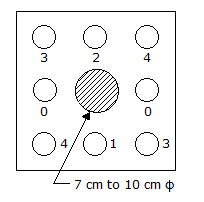
\includegraphics{../data_img/tunnel-engineering_1525415713-33.png}
}
\\\begin{enumerate*}[itemjoin=\qquad, label=\Alph*.]
\item{Michigan cut}
\item{Burn cut}
\item{Fan cut}
\item{Horizontal cut}
\end{enumerate*}
\item{The following operations are required for tunnelling in rocky terrain:  \\
1.Removing the foul gases \\
2.Marking the tunnel profile \\
3.Setting up and drilling \\
4.Checking misfire \\
5.Mucking \\
The correct sequence is:
}
\\\begin{enumerate*}[itemjoin=\qquad, label=\Alph*.]
\item{1, 2, 3, 4, 5}
\item{2, 3, 5, 4, 1}
\item{4, 2, 1, 3, 5}
\item{2, 3, 1, 4, 5}
\end{enumerate*}
\item{The length of the needle beam used in needle beam method of tunnelling is usually}
\\\begin{enumerate*}[itemjoin=\qquad, label=\Alph*.]
\item{2 m to 4 m}
\item{2.5 m to 6 m}
\item{4 m to 7 m}
\item{5 m to 6 m}
\end{enumerate*}
\item{Railway tunnels are generally}
\\\begin{enumerate*}[itemjoin=\qquad, label=\Alph*.]
\item{Polycentric}
\item{Rectangular}
\item{Parabolic}
\item{Circular}
\end{enumerate*}
\item{The method of draining in the tunnels, is generally known as}
\begin{enumerate}[label=\Alph*.]
\item{Foredrainage}
\item{Dewatering}
\item{Permanent drainage}
\item{All of the above}
\end{enumerate}
\item{In the wooded bulk-head, used for mucking in steep grade tunnels,}
\begin{enumerate}[label=\Alph*.]
\item{One opening is provided}
\item{Two openings are provided}
\item{Three openings are provided}
\item{No opening is provided}
\end{enumerate}
\item{Ribs are used for strengthening and stiffening the liner plate for tunnels of diameter greater than}
\\\begin{enumerate*}[itemjoin=\qquad, label=\Alph*.]
\item{2 m}
\item{3 m}
\item{4 m}
\item{5 m}
\end{enumerate*}
\item{For B.G. single track railway, the height of the tunnel above top of rails should be}
\\\begin{enumerate*}[itemjoin=\qquad, label=\Alph*.]
\item{5.5 m to 5.8 m}
\item{5.8 m to 6.2 m}
\item{6.7 m to 7.3 m}
\item{7.3 m to 7.5 m}
\end{enumerate*}
\item{A good blast with a good yield is obtained if the cut hole is}
\begin{enumerate}[label=\Alph*.]
\item{Normal to face}
\item{Inclined at 45$^\circ$ to the face}
\item{Inclined at 15$^\circ$ to the face}
\item{Inclined at 30$^\circ$ to the face}
\end{enumerate}
\item{For initial surveys of tunnels, the following activities are involved: \\
1.Marking portal point with concrete pillars on the ground \\
2.Marking tunnel obligatory points on the topographical maps \\
3.Preliminary setting of the tunnel on the topographical Survey of India maps \\
4.Driving lines between the fixed obligatory points \\
The correct sequence of the activities is:}
\\\begin{enumerate*}[itemjoin=\qquad, label=\Alph*.]
\item{3, 2, 4, 1}
\item{1, 2, 3, 4}
\item{4, 3, 1, 2}
\item{2, 4, 3, 1}
\end{enumerate*}
\item{In Belgium method of tunnelling}
\begin{enumerate}[label=\Alph*.]
\item{Construction of side walls is completed before invert and roof arch are built}
\item{Construction of roof arch is completed before side walls and inverts are built}
\item{Construction of invert is completed before side walls and roof arch are built}
\item{Construction of invert and side walls is completed before roof arch is built}
\end{enumerate}
\item{The advantages of providing a pair of tunnels as compared to only one large highway tunnel is:}
\begin{enumerate}[label=\Alph*.]
\item{Economy in cost of construction}
\item{Avoidance of head on collisions}
\item{Provision of separate exit and entrance of two traffic streams}
\item{All the above}
\end{enumerate}
\item{Which one of the following methods is adopted for permanent drainage of tunnels?}
\begin{enumerate}[label=\Alph*.]
\item{Provision of longitudinal drains}
\item{Continuous open drains}
\item{Concrete lining}
\item{All the above}
\end{enumerate}
\item{What is the correct sequence of the following events of construction of a shaft in rock? \\

1) Drilling and blasting \\

ii) Timbering \\

iii) Pumping \\

iv) Mucking \\

Select the correct answer}
\\\begin{enumerate*}[itemjoin=\qquad, label=\Alph*.]
\item{i, ii, iii, iv}
\item{i, iv, ii, iii}
\item{ii, i, iv, iii}
\item{ii, iv, i, iii}
\end{enumerate*}
\item{Which one of the following is a component of a shield for tunneling?}
\\\begin{enumerate*}[itemjoin=\qquad, label=\Alph*.]
\item{Liner plate}
\item{Trench jack}
\item{Stiffener}
\item{Cutting edge}
\end{enumerate*}
\item{The correct sequence of drilling equipment for increasing size of holes in tunnels is}
\begin{enumerate}[label=\Alph*.]
\item{Wagon drill, churn drill, shot drill}
\item{Wagon drill, shot drill, churn drill}
\item{Shot drill, churn drill, wagon drill}
\item{Churn drill, wagon drill, shot drill}
\end{enumerate}
\item{The difference of heights of the tunnels above rail tops of BG and MG tracks is kept}
\\\begin{enumerate*}[itemjoin=\qquad, label=\Alph*.]
\item{0.30 m}
\item{0.45 m}
\item{0.60 m}
\item{0.75 m}
\end{enumerate*}
\item{For hauling muck from the tunnel, the following type of muck-car is used:}
\\\begin{enumerate*}[itemjoin=\qquad, label=\Alph*.]
\item{Muck box}
\item{Side dump car}
\item{U-bottom}
\item{All of these}
\end{enumerate*}
\item{For B.G. single track, the section of the tunnel must have a width}
\\\begin{enumerate*}[itemjoin=\qquad, label=\Alph*.]
\item{4.2 m to 4.5 m}
\item{4.5 m to 4.8 m}
\item{4.9 m to 5.5 m}
\item{5.5 m to 5.8 m}
\end{enumerate*}
\item{For transferring the tunnel alignment through shafts, we adopt the following steps:  \\
1.Hanging two or more plumb lines in the shaft \\
2.Determining the bearing of the plumb lines i.e. plumb plane \\
3.Suspending a 35 kg weight by each plumb line \\
4.Immersing the weights of both the plumb lines in the buckets containing water \\
The correct sequence of steps is:
}
\\\begin{enumerate*}[itemjoin=\qquad, label=\Alph*.]
\item{1, 2, 3, 4}
\item{4, 3, 2, 1}
\item{1, 3, 2, 4}
\item{2, 1, 4, 3}
\end{enumerate*}
\item{Which one of the following is considered to be an advantage of the heading and benching method of tunnel construction?}
\begin{enumerate}[label=\Alph*.]
\item{It is suitable for construction in unstable rocks}
\item{In this method, it is easy to install timber support}
\item{Tunneling can be continuous and the work can be expedited}
\item{In case of excessive water, it is easy to take correct steps}
\end{enumerate}
\item{Which one of the following methods is generally adopted for tunnelling in firm ground}
\begin{enumerate}[label=\Alph*.]
\item{Full face method}
\item{Top heading and benching method}
\item{Drift method}
\item{All the above}
\end{enumerate}
\item{Which of the following is not a component of the shield?}
\begin{enumerate}[label=\Alph*.]
\item{Propelling jacks}
\item{Liner plate}
\item{Hood}
\item{Tail}
\end{enumerate}
\item{Which one of the following statements is not correct for heading and benching method of tunnelling?}
\begin{enumerate}[label=\Alph*.]
\item{Drilling and mucking can be done simultaneously}
\item{Benching provides a platform for working on heading}
\item{Removal of muck from the heading is very easy}
\item{None of these}
\end{enumerate}
\item{Which one of the following statements is not correct with regard to heading and henching method of tunnelling?}
\begin{enumerate}[label=\Alph*.]
\item{Driving of tunnel is done in two portions of its section}
\item{Driving the top portion is done in advance of the bottom portion}
\item{The holes in head and bench are loaded together with explosive for blasting}
\item{Firing of head holes is done just before the bench holes are fired}
\end{enumerate}
\item{What is the correct sequence of the following events in rock tunnelling? \\

1. Marking tunnel profile \\

2. Loading explosives and blasting \\

3. Checking misfire \\

4. Mucking \\

5. Removing foul gas \\

6. Setting up and drilling \\

7. Guniting \\

Select the correct answer}
\begin{enumerate}[label=\Alph*.]
\item{1, 6, 5, 3, 4, 2, 7}
\item{1, 2, 6, 3, 5, 4, 7}
\item{1, 6, 2, 5, 4, 3, 7}
\item{1, 6, 2, 5, 3, 4, 7}
\end{enumerate}
\item{An overhead track on a large truss frame is required in case of car changer by}
\begin{enumerate}[label=\Alph*.]
\item{The grass hopper method}
\item{The passing track method}
\item{California crossing method}
\item{Dixon conveyor method}
\end{enumerate}
\item{Pick up the explosive used for tunnelling in soft rocks from the following:}
\begin{enumerate}[label=\Alph*.]
\item{Blasting gelatine}
\item{Special gelatine}
\item{Ammonia dynamite}
\item{Semi-gelatine}
\end{enumerate}
\item{Pick up the mechanical ventilation method used for tunnels from the following:}
\begin{enumerate}[label=\Alph*.]
\item{Blowing fresh air by ducts to the face of tunnel}
\item{Exhausting foul air by ducts from the face of the tunnel and permitting fresh air through the tunnel}
\item{Blowing fresh air and exhausting foul air by ducts}
\item{All the above}
\end{enumerate}
\item{Pick up the correct statement regarding drilling a tunnel from the following:}
\begin{enumerate}[label=\Alph*.]
\item{Holes are drilled by pneumatically operated rock drills}
\item{One drill is required for each 4 to 5 m\^{}2 force area}
\item{The diameter of the bore hole at the deepest point should be 6 mm more than the diameter of the cartridge}
\item{All of the above}
\end{enumerate}
\item{Pick up the correct statement from the following:}
\begin{enumerate}[label=\Alph*.]
\item{The topographical maps of the Survey of India are useful in the mountainous region for tunnelling}
\item{The height point on the ridge is fixed with the help of reciprocal ranging}
\item{The accuracy of 1 in 10,000 is required for planimetric control}
\item{All the above}
\end{enumerate}
\item{If `N' is the number of shafts used, then the total number of faces available for attacking the excavation and construction in tunnels are
}
\\\begin{enumerate*}[itemjoin=\qquad, label=\Alph*.]
\item{2N}
\item{N + 2}
\item{2N + 1}
\item{2N + 2}
\end{enumerate*}
\item{For highways, tunnelling is preferred to if the open cut exceeds:}
\begin{enumerate}[label=\Alph*.]
\item{10 meters depth}
\item{15 meters depth}
\item{20 meters depth}
\item{25 meters depth}
\end{enumerate}
\item{Forepoling method is generally adopted for tunnelling in:}
\\\begin{enumerate*}[itemjoin=\qquad, label=\Alph*.]
\item{Soft ground}
\item{Firm ground}
\item{Running ground}
\item{None of these}
\end{enumerate*}
\item{A tunnel is found more advantageous as compared to the alternate routes because it:}
\begin{enumerate}[label=\Alph*.]
\item{Remains free from snow}
\item{Reduces the cost by reducing the route distance}
\item{Reduces the maintenance cost}
\item{All the above}
\end{enumerate}
\item{The needle beam method of tunnelling \\
 (i) Is suitable for soils in which roof can stand for few minutes without support \\
 (ii) Is suitable for brick lining \\
 (iii) Is suitable for concrete lining \\
 (iv) Requires large number of trench jacks}
\begin{enumerate}[label=\Alph*.]
\item{Only (i) is correct}
\item{(i), (ii) and (iv) are correct}
\item{(i), (iii) and (iv) are correct}
\item{(i) and (ii) are correct}
\end{enumerate}
\item{Concrete lining is provided concurrently with the driving operation in case of}
\\\begin{enumerate*}[itemjoin=\qquad, label=\Alph*.]
\item{Rock terrain}
\item{Soft rock}
\item{Running soil}
\item{None of these}
\end{enumerate*}
\item{In ``full face'' method of constructing tunnels, the first operation relates to
}
\begin{enumerate}[label=\Alph*.]
\item{Removal of bottom portion}
\item{Excavation of one drift in the centre}
\item{Removal of top portion}
\item{Excavation being done along the periphery}
\end{enumerate}
\item{The following operations are generally employed for tunnelling in hard rock.  \\
1.Removing ground water,  \\
2.Loading holes and firing the explosive  \\
3.Setting up and drilling  \\
4.Grouting and lining  \\
5.Removing muck  \\
6.Ventilation and removing explosion dust  \\
The correct sequence is:}
\begin{enumerate}[label=\Alph*.]
\item{3, 2, 6, 5, 1, 4}
\item{3, 4, 6, 1, 5, 2}
\item{4, 1, 2, 3, 6, 5}
\item{5, 4, 2, 1, 3, 6}
\end{enumerate}
\item{In the given figure drill holes, heading, mucking and benching are numbered as 1, 2, 3, 4; The correct sequence is: \\
 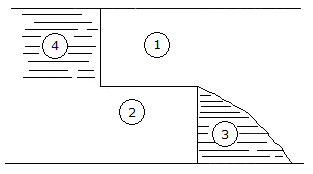
\includegraphics{../data_img/tunnel-engineering_1525415833-32.png}
}
\\\begin{enumerate*}[itemjoin=\qquad, label=\Alph*.]
\item{4, 1, 2, 3}
\item{1, 2, 3, 4}
\item{4, 1, 3, 2}
\item{3, 4, 1, 3}
\end{enumerate*}
\item{American method of tunnelling \\
 (i) Is suitable for large sized tunnels \\
 (ii) Is not suitable for railway or highway tunnels \\
 (iii) Requires heavy timbers}
\begin{enumerate}[label=\Alph*.]
\item{Only (i) is correct}
\item{(i) and (iii) are correct}
\item{(ii) and (iii) are correct}
\item{(i) and (ii) are correct}
\end{enumerate}
\item{If `D' is the diameter of tunnel in meters, then the thickness of lining in mm, as per the empirical formula is given by
}
\\\begin{enumerate*}[itemjoin=\qquad, label=\Alph*.]
\item{42 D}
\item{82 D}
\item{104 D}
\item{124 D}
\end{enumerate*}
\item{As compared to a single free face, if a charge of explosive is placed equidistant from two faces, then the yield}
\begin{enumerate}[label=\Alph*.]
\item{Remain same}
\item{Decreases}
\item{Increases by 2.25 times}
\item{Increases by 3.5 times}
\end{enumerate}
\item{Assertion A: When rock conditions are favorable, it will not be necessary to take up concrete lining concurrently with the driving operations till the full length of the tunnel has been driven through rock. \\
Reason R: A tunnel through rock, hard or soft, does not need any concrete lining \\
Select your answer}
\begin{enumerate}[label=\Alph*.]
\item{Both A and R is true and R is the correct explanation of A}
\item{Both A and R is true but R is not the correct explanation of A}
\item{A is true but R is false}
\item{A is false but R is true}
\end{enumerate}
\item{Assertion A: English method of tunnelling requires more time as compared to other methods of tunnelling. \\
Reason R: In English method of tunnelling, the masons and excavators have to work alternately \\

Select your answer}
\begin{enumerate}[label=\Alph*.]
\item{Both A and R is true and R is the correct explanation of A}
\item{Both A and R is true and R is not the correct explanation of A}
\item{A is true but R is false}
\item{A is false but R is true}
\end{enumerate}
\item{Drift method of tunneling is used to construct tunnels in}
\begin{enumerate}[label=\Alph*.]
\item{Soft grounds}
\item{Rock}
\item{Self supporting grounds}
\item{Broken grounds}
\end{enumerate}
\item{The following tunnels were constructed in different countries for different purposes:  \\
1.Emperor Claudius built the first Roman tunnel \\
2.The first highway tunnel was constructed in Hungary \\
3.The first underground railway tunnel was constructed in Great Britain \\
4.The first navigational tunnel was constructed in France. \\
The correct chronological development of these tunnels is:}
\\\begin{enumerate*}[itemjoin=\qquad, label=\Alph*.]
\item{4, 1, 3, 2}
\item{1, 4, 2, 3}
\item{2, 3, 1, 4}
\item{3, 2, 4, 1}
\end{enumerate*}
\item{Pick up the correct statement from the following during tunnel excavation,}
\begin{enumerate}[label=\Alph*.]
\item{Oxygen should not be less than 19.5\%}
\item{Carbondioxide should not be more than 0.5\%}
\item{Hydrogen sulphide should not be more than 0.001\%}
\item{All of the above}
\end{enumerate}
\item{In case of drift method of tunnelling, the drift may be excavated at}
\begin{enumerate}[label=\Alph*.]
\item{The centre}
\item{The top or bottom}
\item{The side}
\item{All of the above}
\end{enumerate}
\end{enumerate}
\textbf{Answer Key}
\begin{tabular}{ | c | c c c c c c c c c c | }
\hline
 & 1 & 2 & 3 & 4 & 5 & 6 & 7 & 8 & 9 & 0 \\
\hline
0 & B & C & C & D & D & D & D & D & D & D \\
10 & D & B & C & B & D & C & C & C & B & B \\
20 & D & A & D & D & A & D & B & B & C & B \\
30 & A & B & D & D & B & D & A & C & D & C \\
40 & A & C & D & B & C & D & D & A & C & D \\
50 & D & D & D & B & A & D & B & A & D & A \\
60 & C & A & B & C & C & A & B & B & D & D \\
\hline
\end{tabular}
\clearpage
\section{Surveying}
\subsection*{Section 1}
\begin{enumerate}
\item{If 16 flight lines are run perpendicular to an area 30 km wide, their spacings on a photographical map on scale 1 : 50,000 , will be}
\\\begin{enumerate*}[itemjoin=\qquad, label=\Alph*.]
\item{1 cm}
\item{2 cm}
\item{3 cm}
\item{4 cm}
\end{enumerate*}
\item{Which of the following methods of contouring is most suitable for a hilly terrain?}
\begin{enumerate}[label=\Alph*.]
\item{Direct method}
\item{Square method}
\item{Cross-sections method}
\item{Tachometric method}
\end{enumerate}
\item{The size of a plane table is}
\begin{enumerate}[label=\Alph*.]
\item{750 mm $\times$ 900 mm}
\item{600 mm $\times$ 750 mm}
\item{450 mm $\times$ 600 mm}
\item{300 mm $\times$ 450 mm}
\end{enumerate}
\item{The angle between the plane of the equator and the plane of the ecliptic, is known as obliquity of the ecliptic and its value is}
\\\begin{enumerate*}[itemjoin=\qquad, label=\Alph*.]
\item{22$^\circ$ 30'}
\item{23$^\circ$ 27'}
\item{23$^\circ$ 30'}
\item{24$^\circ$ 0'}
\end{enumerate*}
\item{For a tacheometer the additive and multi-plying constants are respectively}
\\\begin{enumerate*}[itemjoin=\qquad, label=\Alph*.]
\item{0 and 100}
\item{100 and 0}
\item{0 and 0}
\item{100 and 100}
\end{enumerate*}
\item{From the principal point the horizon point lies on the principal line at a distance of}
\\\begin{enumerate*}[itemjoin=\qquad, label=\Alph*.]
\item{f tan $\theta$}
\item{f sin $\theta$}
\item{f cot $\theta$}
\item{f cos $\theta$}
\end{enumerate*}
\item{If the magnetic bearing of the sun at a place at noon in southern hemisphere is 167$^\circ$, the magnetic declination at that place is
}
\\\begin{enumerate*}[itemjoin=\qquad, label=\Alph*.]
\item{77$^\circ$ N}
\item{23$^\circ$ S}
\item{13$^\circ$ E}
\item{13$^\circ$ W}
\end{enumerate*}
\item{Overturning of vehicles on a curve can be avoided by using}
\begin{enumerate}[label=\Alph*.]
\item{compound curve}
\item{vertical curve}
\item{reverse curve}
\item{transition curve}
\end{enumerate}
\item{The error due to eccentricity of inner and outer axes can be eliminated by}
\begin{enumerate}[label=\Alph*.]
\item{reading both verniers and taking the mean of the two}
\item{taking both face observations and taking the mean of the two}
\item{double sighting}
\item{taking mean of several readings distributed over different portions of the graduated circle}
\end{enumerate}
\item{The Polaris remains below horizon at}
\\\begin{enumerate*}[itemjoin=\qquad, label=\Alph*.]
\item{10$^\circ$ N}
\item{50$^\circ$ N Latitude}
\item{Equator}
\item{5$^\circ$ S latitude}
\end{enumerate*}
\item{Three point problem can be solved by}
\begin{enumerate}[label=\Alph*.]
\item{Tracing paper method}
\item{Bessels method}
\item{Lehman's method}
\item{all of the above}
\end{enumerate}
\item{The zenith is the point on the celestial sphere}
\begin{enumerate}[label=\Alph*.]
\item{East of observer}
\item{West of observer}
\item{North of observer}
\item{South of observer}
\end{enumerate}
\item{The allowable length of an offset depends upon the}
\begin{enumerate}[label=\Alph*.]
\item{degree of accuracy required}
\item{method of setting out the perpendiculars and nature of ground}
\item{scale of plotting}
\item{all of the above}
\end{enumerate}
\item{The great circle whose plane is perpendicular to the axis of rotation of the earth, is called}
\begin{enumerate}[label=\Alph*.]
\item{Equator}
\item{Terrestrial equator}
\item{0$^\circ$ latitude}
\item{All the above}
\end{enumerate}
\item{The plane at right angle to the zenith-nadir line and passing through the centre of the earth, is called}
\begin{enumerate}[label=\Alph*.]
\item{Rational horizon}
\item{True horizon}
\item{Celestial horizon}
\item{All the above}
\end{enumerate}
\item{To obtain photographs of an area of 1000 m average elevation, on scale 1 : 30,000, with a camera of 30 cm focal length, the flying height is}
\\\begin{enumerate*}[itemjoin=\qquad, label=\Alph*.]
\item{4000 m}
\item{5000 m}
\item{6000 m}
\item{7000 m}
\end{enumerate*}
\item{The difference of height of two points whose parallax difference is 0.8 mm on a pair of stereo pair taken from a height `H' is 100 m. If mean photo base is 95.2 mm, the flying height is
}
\\\begin{enumerate*}[itemjoin=\qquad, label=\Alph*.]
\item{8,000 m}
\item{10,000 m}
\item{12,000 m}
\item{14,000 m}
\end{enumerate*}
\item{The correction for parallax, is}
\\\begin{enumerate*}[itemjoin=\qquad, label=\Alph*.]
\item{- 8".8 cos $\alpha$}
\item{+ .8" sin $\alpha$}
\item{+ 8".8 cos $\alpha$}
\item{- 8".8 cos $\alpha$}
\end{enumerate*}
\item{The Polaris describes a small circle round the pole whose radius is approximately}
\\\begin{enumerate*}[itemjoin=\qquad, label=\Alph*.]
\item{1$^\circ$}
\item{2$^\circ$}
\item{3$^\circ$}
\item{4$^\circ$}
\end{enumerate*}
\item{Sensitiveness of a level tube is designated by}
\begin{enumerate}[label=\Alph*.]
\item{radius of level tube}
\item{length of level tube}
\item{length of bubble of level tube}
\item{none of the above}
\end{enumerate}
\item{Agate cap is fitted with a}
\begin{enumerate}[label=\Alph*.]
\item{cross staff}
\item{level}
\item{chain}
\item{prismatic compass}
\end{enumerate}
\item{International Date Line is located along}
\begin{enumerate}[label=\Alph*.]
\item{Standard meridian}
\item{Greenwich meridian}
\item{Equator}
\item{180$^\circ$ longitude}
\end{enumerate}
\item{The length of a chain is measured from}
\begin{enumerate}[label=\Alph*.]
\item{centre of one handle to centre of other handle}
\item{outside of one handle to outside of other handle}
\item{outside of one handle to inside of other handle}
\item{inside of one handle to inside of other handle}
\end{enumerate}
\item{The nautical mile is the length of}
\begin{enumerate}[label=\Alph*.]
\item{1 minute of latitude}
\item{1 minute of longitude}
\item{1 degree of latitude}
\item{1 degree of longitude}
\end{enumerate}
\item{If the equatorial distance between two meridians is 100 km, their distance at 60$^\circ$ latitude will be
}
\\\begin{enumerate*}[itemjoin=\qquad, label=\Alph*.]
\item{1000 km}
\item{800 km}
\item{600 km}
\item{500 km}
\end{enumerate*}
\item{The scale of the photography taken from a height of 300 m, with a camera of focal length 15 cm, is}
\\\begin{enumerate*}[itemjoin=\qquad, label=\Alph*.]
\item{1 : 10,000}
\item{1 : 15,000}
\item{1 : 20,000}
\item{1 : 30,000}
\end{enumerate*}
\item{In an internal focussing type of telescope, the lens provided is}
\\\begin{enumerate*}[itemjoin=\qquad, label=\Alph*.]
\item{concave}
\item{convex}
\item{plano-convex}
\item{plano-concave}
\end{enumerate*}
\item{Which of the following is not the function of levelling head ?}
\begin{enumerate}[label=\Alph*.]
\item{to support the main part of the instrument}
\item{to attach the theodolite to the tripod}
\item{to provide a means for leveling the theodolite}
\item{none of the above}
\end{enumerate}
\item{Local attraction in compass surveying may exist due to}
\begin{enumerate}[label=\Alph*.]
\item{incorrect levelling of the magnetic needle}
\item{loss of magnetism of the needle}
\item{friction of the needle at the pivot}
\item{presence of magnetic substances near the instrument}
\end{enumerate}
\item{A Nautical mile is}
\begin{enumerate}[label=\Alph*.]
\item{One minute arc of the great circle passing through two points}
\item{One minute arc of the longitude}
\item{1855.109 m}
\item{All the above}
\end{enumerate}
\item{With the rise of temperature, the sensitivity of a bubble tube}
\begin{enumerate}[label=\Alph*.]
\item{decreases}
\item{increases}
\item{remains unaffected}
\item{none of the above}
\end{enumerate}
\item{Direct method of contouring is}
\begin{enumerate}[label=\Alph*.]
\item{a quick method}
\item{adopted for large surveys only}
\item{most accurate method}
\item{suitable for hilly terrains}
\end{enumerate}
\item{The correction applied to the measured base of length `L' is
}
\begin{enumerate}[label=\Alph*.]
\item{Tension $$ = \frac{{\left( {{\text{P}} - {{\text{P}}\_{\text{s}}}} \right){\text{L}}}}{{{\text{AE}}}}$$}
\item{Sag $$ = \frac{{{{\text{L}}^3}{{\text{w}}^2}}}{{24{{\text{P}}^2}}}$$ ~where w is the weight of tape/m}
\item{Slope $$ = \frac{{{{\text{h}}^2}}}{{2{\text{L}}}} + \frac{{{{\text{h}}^4}}}{{8{{\text{L}}^3}}}$$ ~ where h is height difference of end supports}
\item{Reduction to mean sea level $$ = \frac{{{\text{Lh}}}}{{\text{R}}}$$}
\item{All the above}
\end{enumerate}
\item{The shortest distance between two places measured along the surface of the earth, is}
\begin{enumerate}[label=\Alph*.]
\item{Length of the equator between their longitudes}
\item{Length of the parallel between their longitudes}
\item{Length of the arc of the great circle passing through them}
\item{None of these}
\end{enumerate}
\item{Longitude of a place is the angular distance between the meridian of the place and}
\begin{enumerate}[label=\Alph*.]
\item{The standard meridian}
\item{The International Date Line}
\item{That of Greenwich}
\item{Both (A) and (C) of above}
\end{enumerate}
\item{If the altitudes of a star at its upper and lower transits are 60$^\circ$ 30' and 19$^\circ$ 30' respectively, the latitude of the place, is
}
\\\begin{enumerate*}[itemjoin=\qquad, label=\Alph*.]
\item{30$^\circ$}
\item{35$^\circ$}
\item{30$^\circ$}
\item{45$^\circ$}
\end{enumerate*}
\item{The altitudes of a circumpolar star at culminations are 70$^\circ$ and 10$^\circ$, both culminations being north of zenith. The latitude of the place, is
}
\\\begin{enumerate*}[itemjoin=\qquad, label=\Alph*.]
\item{80$^\circ$}
\item{70$^\circ$}
\item{60$^\circ$}
\item{40$^\circ$}
\end{enumerate*}
\item{Triangulation surveys are carried out for locating}
\begin{enumerate}[label=\Alph*.]
\item{Control points for surveys of large areas}
\item{Control points for photogrammetric surveys}
\item{Engineering works, i.e. terminal points of long tunnels, bridge abutments, etc.}
\item{All the above}
\end{enumerate}
\item{For plane ground the scale of a vertical photograph will be same as that of a tiled photograph along the photo parallel through}
\begin{enumerate}[label=\Alph*.]
\item{Isocenter}
\item{Plumb point}
\item{Principal point}
\item{None of these}
\end{enumerate}
\item{If the general ground level of any area is 10\% of the flying height, the principal points may be used as the centers of radial directions for small scale mapping even in tilted photograph up to}
\\\begin{enumerate*}[itemjoin=\qquad, label=\Alph*.]
\item{1$^\circ$}
\item{2$^\circ$}
\item{3$^\circ$}
\item{4$^\circ$}
\end{enumerate*}
\item{A star is said to elongate}
\begin{enumerate}[label=\Alph*.]
\item{When the star momentarily moves vertically}
\item{When the angle at the star of the spherical triangle is 90$^\circ$}
\item{When the star}
\item{All the above}
\end{enumerate}
\item{If the intercept on a vertical staff is ob-served as 0.75 m from a tacheometer, the horizontal distance between tacheometer and staff station is}
\\\begin{enumerate*}[itemjoin=\qquad, label=\Alph*.]
\item{7.5 m}
\item{25 m}
\item{50 m}
\item{75 m}
\end{enumerate*}
\item{The latitude of a place was obtained by subtracting the zenith distance of a star from its declination, the observed star was between}
\begin{enumerate}[label=\Alph*.]
\item{Horizon and equator}
\item{Equator and zenith}
\item{Zenith and pole}
\item{Pole and horizon}
\end{enumerate}
\item{The latitude of a place was obtained by subtracting the declination of a star from its zenith distance, the observed star was between}
\begin{enumerate}[label=\Alph*.]
\item{Horizon and equator}
\item{Zenith and pole}
\item{Equator and zenith}
\item{Pole and horizon}
\end{enumerate}
\item{The flying height of the camera is 1,000 m above mean ground level, the distance of the top of a building from a nadir point is 10 cm and the relief displacement of building is 7.2 mm. The height of the building, is}
\\\begin{enumerate*}[itemjoin=\qquad, label=\Alph*.]
\item{52 m}
\item{62 m}
\item{72 m}
\item{82 m}
\end{enumerate*}
\item{The stereo plotting instruments are generally manufactured on the principle of}
\begin{enumerate}[label=\Alph*.]
\item{Optical projection}
\item{Optical mechanism projection}
\item{Mechanical projection}
\item{All the above}
\end{enumerate}
\item{The true and mean suns occupy the same meridian at the same time on}
\\\begin{enumerate*}[itemjoin=\qquad, label=\Alph*.]
\item{April 15}
\item{June 14}
\item{September 1}
\item{All the above}
\end{enumerate*}
\item{If E is the spherical excess and R the radius of the earth, the surface area of the triangle, is}
\\\begin{enumerate*}[itemjoin=\qquad, label=\Alph*.]
\item{$ \frac{{\pi {{\text{R}}^2}{\text{E}}}}{{{{90}^ \circ }}} $}
\item{$ \frac{{\pi {{\text{R}}^2}{\text{E}}}}{{{{180}^ \circ }}} $}
\item{$ \frac{{\pi {{\text{R}}^2}{\text{E}}}}{{{{270}^ \circ }}} $}
\item{$ \frac{{\pi {{\text{R}}^2}{\text{E}}}}{{{{360}^ \circ }}} $}
\end{enumerate*}
\item{The station which is selected close to the main triangulation station, to avoid intervening obstruction, is not known as}
\begin{enumerate}[label=\Alph*.]
\item{Satellite station}
\item{Eccentric station}
\item{False station}
\item{Pivot station}
\end{enumerate}
\item{In a spherical triangle ABC right angled at C, sin b equals to}
\\\begin{enumerate*}[itemjoin=\qquad, label=\Alph*.]
\item{sin c sin B}
\item{cos c cos B}
\item{tan c tan B}
\item{sin c cos B}
\end{enumerate*}
\item{23 cm $\times$ 23 cm photographs are taken from a flying height with a camera of focal length of 3600 m and 15.23 cm respectively. A parallax difference of 0.01 mm represents
}
\\\begin{enumerate*}[itemjoin=\qquad, label=\Alph*.]
\item{1 m}
\item{2 m}
\item{4 m}
\item{8 m}
\end{enumerate*}
\item{The declination and right ascension of the sun becomes 23$^\circ$ 27' N and 90$^\circ$ respectively on
}
\\\begin{enumerate*}[itemjoin=\qquad, label=\Alph*.]
\item{March 21}
\item{June 21}
\item{September 21}
\item{December 22}
\end{enumerate*}
\item{The declination and right ascension of the sun becomes 23$^\circ$ 27' S and 270$^\circ$ respectively on
}
\\\begin{enumerate*}[itemjoin=\qquad, label=\Alph*.]
\item{March 21}
\item{June 21}
\item{September 21}
\item{December 22}
\end{enumerate*}
\item{The following sights are taken on a ``turning point''
}
\begin{enumerate}[label=\Alph*.]
\item{foresight only}
\item{backsight only}
\item{foresight and backsight}
\item{foresight and intermediate sight}
\end{enumerate}
\item{The horizontal angle between the true meridian and magnetic meridian at a place is called}
\begin{enumerate}[label=\Alph*.]
\item{azimuth}
\item{declination}
\item{local attraction}
\item{magnetic bearing}
\end{enumerate}
\item{A 'level line' is a
}
\begin{enumerate}[label=\Alph*.]
\item{horizontal line}
\item{line parallel to the mean spheriodal surface of earth}
\item{line passing through the center of cross hairs and the center of eye piece}
\item{line passing through the objective lens and the eye-piece of a dumpy or tilting level}
\end{enumerate}
\item{Accidental errors}
\begin{enumerate}[label=\Alph*.]
\item{Do not follow any definite mathematical law}
\item{Cannot be removed by applying corrections to the observed values}
\item{Are generally small}
\item{All the above}
\end{enumerate}
\item{Pick up the correct statement from the following. The difference between the longitudes of the places is obtained.}
\begin{enumerate}[label=\Alph*.]
\item{By subtracting their longitudes if places are in the same hemisphere}
\item{By adding their longitudes if places are in the different hemispheres}
\item{By subtracting the sum of their longitudes exceeding 180$^\circ$ from 360$^\circ$ if places are in different hemispheres}
\item{All the above}
\end{enumerate}
\item{Refraction correction}
\begin{enumerate}[label=\Alph*.]
\item{completely eliminates curvature correction}
\item{partially eliminates curvature correction}
\item{adds to the curvature correction}
\item{has no effect on curvature correction}
\end{enumerate}
\item{The number of horizontal cross wires in a stadia diaphragm is}
\\\begin{enumerate*}[itemjoin=\qquad, label=\Alph*.]
\item{one}
\item{two}
\item{three}
\item{four}
\end{enumerate*}
\item{The prime vertical passes through}
\begin{enumerate}[label=\Alph*.]
\item{The east point of the horizon}
\item{The west point of the horizon}
\item{The zenith point of the observer}
\item{All the above}
\end{enumerate}
\item{The relation between the air base (B), photographic base (b), flying height (H) and the focal length (f) of a vertical photograph, is}
\\\begin{enumerate*}[itemjoin=\qquad, label=\Alph*.]
\item{$ {\text{B}} = \frac{{{\text{bH}}}}{{\text{f}}} $}
\item{$ {\text{B}} = \frac{{\text{f}}}{{{\text{bH}}}} $}
\item{$ {\text{B}} = \frac{{\text{b}}}{{{\text{fH}}}} $}
\item{$ {\text{B}} = \frac{{\text{H}}}{{{\text{bf}}}} $}
\end{enumerate*}
\item{The principal plane contains}
\begin{enumerate}[label=\Alph*.]
\item{Nadir point}
\item{Iso-centre}
\item{Principal point}
\item{All the above}
\end{enumerate}
\item{Latitude of the observer's position is equal to altitude of}
\\\begin{enumerate*}[itemjoin=\qquad, label=\Alph*.]
\item{North pole}
\item{Pole star}
\item{Celestial pole}
\item{All the above}
\end{enumerate*}
\item{The parallax equation $$\Delta {\text{p}} = \frac{{{\text{Bm}}\Delta {\text{h}}}}{{{\text{H}} - {\text{h}}}}$$ ~ is applicable to entire overlap of the photographs only if parallax is measured
}
\begin{enumerate}[label=\Alph*.]
\item{Normal to base line}
\item{Parallel to base line}
\item{Both (A) and (B)}
\item{Neither (A) nor (B)}
\end{enumerate}
\item{If the length of a chain is found to be short on testing, it can be adjusted by}
\begin{enumerate}[label=\Alph*.]
\item{straightening the links}
\item{removing one or more small circular rings}
\item{closing the joints of the rings if opened out}
\item{all of the above}
\end{enumerate}
\item{In the double application of principle of reversion, the apparent error is}
\begin{enumerate}[label=\Alph*.]
\item{equal to true error}
\item{half the true error}
\item{two times the true error}
\item{four times the true error}
\end{enumerate}
\item{The solar tidal force divided by lunar tidal force is}
\\\begin{enumerate*}[itemjoin=\qquad, label=\Alph*.]
\item{$ \frac{1}{3} $}
\item{$ \frac{1}{2} $}
\item{$ \frac{3}{4} $}
\item{$ \frac{5}{4} $}
\end{enumerate*}
\item{Closed contours, with higher value inwards, represent a}
\begin{enumerate}[label=\Alph*.]
\item{depression}
\item{hillock}
\item{plain surface}
\item{none of the above}
\end{enumerate}
\item{The average eye base is assumed as}
\\\begin{enumerate*}[itemjoin=\qquad, label=\Alph*.]
\item{58 mm}
\item{60 mm}
\item{62 mm}
\item{64 mm}
\end{enumerate*}
\end{enumerate}
\textbf{Answer Key}
\begin{tabular}{ | c | c c c c c c c c c c | }
\hline
 & 1 & 2 & 3 & 4 & 5 & 6 & 7 & 8 & 9 & 0 \\
\hline
0 & D & D & B & B & A & A & C & D & A & D \\
10 & D & D & D & D & D & C & C & C & A & A \\
20 & D & D & B & B & D & C & A & D & D & D \\
30 & A & C & E & C & D & C & D & D & A & C \\
40 & D & D & C & A & C & D & D & B & D & A \\
50 & A & B & D & C & B & B & D & C & B & C \\
60 & D & A & D & C & B & A & D & B & B & D \\
\hline
\end{tabular}
\clearpage
\subsection*{Section 2}
\begin{enumerate}
\item{Longitudes are measured from 0$^\circ$ to
}
\begin{enumerate}[label=\Alph*.]
\item{180$^\circ$ eastward}
\item{180$^\circ$ westward}
\item{180$^\circ$ east or westward}
\item{360$^\circ$ eastward}
\end{enumerate}
\item{If `$\delta$' is the declination of the star and `$\phi$' is the latitude of the observer then the hour angle of the star at elongation is given by
}
\begin{enumerate}[label=\Alph*.]
\item{sin H = tan $\phi$ . cot $\delta$}
\item{cos H = tan $\phi$ . cot $\delta$}
\item{tan H = tan $\phi$ . cot $\delta$}
\item{None of these}
\end{enumerate}
\item{If `$\delta$' is the declination of the star and `$\phi$' is the latitude of the observer, then the azimuth of the star at elongation is given by
}
\begin{enumerate}[label=\Alph*.]
\item{sin z = sec $\phi$ . cos $\delta$}
\item{cos z = sec $\phi$ . cos $\delta$}
\item{tan z = sec $\phi$ . cos $\delta$}
\item{None of these}
\end{enumerate}
\item{The altitude of a circumpolar star is maximum when it is}
\begin{enumerate}[label=\Alph*.]
\item{At east elongation}
\item{At upper culmination}
\item{At west elongation}
\item{At lower culmination}
\end{enumerate}
\item{Rotation of the camera at exposure about its vertical axis, is known as}
\\\begin{enumerate*}[itemjoin=\qquad, label=\Alph*.]
\item{Swing}
\item{Tilt}
\item{Tip}
\item{None of these}
\end{enumerate*}
\item{The angle between the observer's meridian and declination circle of a heavenly body, is known as}
\begin{enumerate}[label=\Alph*.]
\item{Hour angle}
\item{Azimuth}
\item{Right ascension}
\item{Declination}
\end{enumerate}
\item{A metallic tape is made of}
\begin{enumerate}[label=\Alph*.]
\item{steel}
\item{invar}
\item{linen}
\item{cloth and wires}
\end{enumerate}
\item{If S is the sum of three angles of a spherical triangle, the spherical excess equals}
\\\begin{enumerate*}[itemjoin=\qquad, label=\Alph*.]
\item{S - 90$^\circ$}
\item{S - 180$^\circ$}
\item{S - 270$^\circ$}
\item{S - 360$^\circ$}
\end{enumerate*}
\item{The suitable contour interval for a map with scale 1 : 10000 is}
\\\begin{enumerate*}[itemjoin=\qquad, label=\Alph*.]
\item{2 m}
\item{5 m}
\item{10 m}
\item{20 m}
\end{enumerate*}
\item{Which of the following methods of plane table surveying is used to locate the position of an inaccessible point ?}
\\\begin{enumerate*}[itemjoin=\qquad, label=\Alph*.]
\item{radiation}
\item{intersection}
\item{traversing}
\item{resection}
\end{enumerate*}
\item{Which of the following errors cannot be eliminated by taking both face observations ?}
\begin{enumerate}[label=\Alph*.]
\item{error due to horizontal axis not being perpendicular to the vertical axis}
\item{index error i.e. error due to imperfect adjustment of the vertical circle vernier}
\item{error due to non-parallelism of the axis of telescope level and line of collimation}
\item{none of the above}
\end{enumerate}
\item{Which of the following errors can be eliminated by taking mean of bot face observations ?}
\begin{enumerate}[label=\Alph*.]
\item{error due to imperfect graduations}
\item{error due to eccentricity of verniers}
\item{error due to imperfect adjustment of plate levels}
\item{error due to line of collimation not being perpendicular to horizontal axis}
\end{enumerate}
\item{The scale of a vertical photograph of focal length `f' taken from height of `H' metres above M.S.L., at a point of reduced level `h', is
}
\\\begin{enumerate*}[itemjoin=\qquad, label=\Alph*.]
\item{$ \frac{{\text{f}}}{{\text{H}}} $}
\item{$ \frac{{\text{f}}}{{{\text{H}} + {\text{h}}}} $}
\item{$ \frac{{\text{f}}}{{{\text{H}} - {\text{h}}}} $}
\item{$ \frac{{{\text{H}} - {\text{h}}}}{{\text{f}}} $}
\end{enumerate*}
\item{Perspective centre relates to}
\begin{enumerate}[label=\Alph*.]
\item{Parallel projection}
\item{Orthogonal projection}
\item{Central projection}
\item{None of these}
\end{enumerate}
\item{Circumpolar stars}
\begin{enumerate}[label=\Alph*.]
\item{Rotate round the North Pole}
\item{Rotate round the celestial pole}
\item{Remain always above the horizon}
\item{Are seldom seen near the pole star}
\end{enumerate}
\item{The rise and fall method of levelling provides a complete check on}
\begin{enumerate}[label=\Alph*.]
\item{backsight}
\item{intermediate sight}
\item{foresight}
\item{all of the above}
\end{enumerate}
\item{Invar tapes used for measuring base lines, is made of nickel-iron alloy containing nickel}
\\\begin{enumerate*}[itemjoin=\qquad, label=\Alph*.]
\item{24 \%}
\item{36 \%}
\item{40 \%}
\item{60 \%}
\end{enumerate*}
\item{In direct method of contouring, the process of locating or identifying points lying on a contour is called}
\begin{enumerate}[label=\Alph*.]
\item{ranging}
\item{centring}
\item{horizontal control}
\item{vertical control}
\end{enumerate}
\item{If altitude bubble is provided both on index frame as well as on telescope of a theodolite, then the instrument is levelled with reference to \\
i) altitude bubble on index frame \\
ii) altitude bubble on index frame if it is to be used as a level \\
iii) altitude bubble on telescope \\
iv) altitude bubble on telescope if it is to be used as a level  \\
The correct answer is}
\begin{enumerate}[label=\Alph*.]
\item{only (i)}
\item{both (i) and (iv)}
\item{only (iii)}
\item{both (ii) and (iii)}
\end{enumerate}
\item{In the cross-section method of indirect contouring, the spacing of cross-sections depends upon \\
i) contour interval \\
ii) scale of plan \\
iii) characteristics of ground \\
The correct answer is}
\begin{enumerate}[label=\Alph*.]
\item{only (i)}
\item{(i) and (ii)}
\item{(ii) and (iii)}
\item{(i), (ii) and (iii)}
\end{enumerate}
\item{Height of instrument method of levelling is}
\begin{enumerate}[label=\Alph*.]
\item{more accurate than rise and fall method}
\item{less accurate than rise and fall method}
\item{quicker and less tedious for large number of intermediate sights}
\item{none of the above}
\end{enumerate}
\item{The slotted template method}
\begin{enumerate}[label=\Alph*.]
\item{Is prepared, by graphical method}
\item{Is suitable for large areas with less control}
\item{Is rapid and accurate}
\item{All the above}
\end{enumerate}
\item{When a star is between the pole and the horizon, the relationship between latitude ($\lambda$), zenith distance (z) and declination $\delta$, is
}
\begin{enumerate}[label=\Alph*.]
\item{$\theta$ = z + $\delta$}
\item{$\theta$ = $\delta$ - z}
\item{$\theta$ = 180$^\circ$ - (z + $\delta$)}
\item{$\theta$ = (z + $\delta$) - 180$^\circ$}
\end{enumerate}
\item{The length of a parallel of $\lambda$ latitude between two meridians is equal to difference in longitudes multiplied by
}
\\\begin{enumerate*}[itemjoin=\qquad, label=\Alph*.]
\item{sin $\lambda$}
\item{cos $\lambda$}
\item{tan $\lambda$}
\item{cot $\lambda$}
\end{enumerate*}
\item{The hour angle of the heavenly body for Greenwich meridian equals the hour angle of the body for any other meridian + longitude:}
\\\begin{enumerate*}[itemjoin=\qquad, label=\Alph*.]
\item{Mean sun}
\item{True sun}
\item{Vernal equinox}
\item{All the above}
\end{enumerate*}
\item{Which of the following is not used in measuring perpendicular offsets ?}
\\\begin{enumerate*}[itemjoin=\qquad, label=\Alph*.]
\item{line ranger}
\item{steel tape}
\item{optical square}
\item{cross staff}
\end{enumerate*}
\item{The nearest star is so far away from the earth that the directions to it from two diametrically opposite points on the earth differs less than}
\\\begin{enumerate*}[itemjoin=\qquad, label=\Alph*.]
\item{0.01 second}
\item{0.001 second}
\item{0.0001 second}
\item{None of these}
\end{enumerate*}
\item{Right ascension of a heavenly body is its equatorial angular distance measured}
\begin{enumerate}[label=\Alph*.]
\item{Westward from the first point of Libra}
\item{Eastward from the first point of Aeries}
\item{Westward from the first point of Aeries}
\item{Eastward from the first point of Libra}
\end{enumerate}
\item{$ \alpha $$ and $$\beta $$ are the angles subtended by a point of elevation h at their air station with respective plumb points. Photo scale and focal length of the lens being ‘S’ and ‘f’ respectively. Parallax displacement of the point due to relief, i $}
\\\begin{enumerate*}[itemjoin=\qquad, label=\Alph*.]
\item{$ \frac{{{\text{h}}\tan \alpha }}{{\text{S}}} $}
\item{$ \frac{{{\text{h}}\tan \beta }}{{\text{S}}} $}
\item{$ \frac{{{\text{h}}\left( {\tan \alpha + \tan \beta } \right)}}{{\text{S}}} $}
\item{$ \frac{{{\text{h}}\left( {\tan \alpha - \tan \beta } \right)}}{{\text{S}}} $}
\end{enumerate*}
\item{The method of surveying by triangulation was first introduced by the Dutchman Snell in}
\\\begin{enumerate*}[itemjoin=\qquad, label=\Alph*.]
\item{1600}
\item{1615}
\item{1630}
\item{1650}
\end{enumerate*}
\item{The rise and fall method}
\begin{enumerate}[label=\Alph*.]
\item{is less accurate than height of instrument method}
\item{is not suitable for levelling with tilting levels}
\item{provides a check on the reduction of intermediate point levels}
\item{quicker and less tedious for large number of intermediate sights}
\end{enumerate}
\item{A telescope is said to be inverted if its}
\begin{enumerate}[label=\Alph*.]
\item{vertical circle is to its right and the bubble of the telescope is down}
\item{vertical circle is to its right and the bubble of the telescope is up}
\item{vertical circle is to its left and the bubble of the telescope is down}
\item{vertical circle is to its left and the bubble of the telescope is up}
\end{enumerate}
\item{Size of a theodolite is specified by}
\begin{enumerate}[label=\Alph*.]
\item{the length of telescope}
\item{the diameter of vertical circle}
\item{the diameter of lower plate}
\item{the diameter of upper plate}
\end{enumerate}
\item{If the reduced bearing of a line AB is N 60$^\circ$ W and length is 100 m, then the latitude and departure respectively of the line AB will be
}
\\\begin{enumerate*}[itemjoin=\qquad, label=\Alph*.]
\item{+50 m, +86.6 m}
\item{+86.6 m, -50 m}
\item{+50 m, -86.6 m}
\item{+70.7 m, -50 m}
\end{enumerate*}
\item{A lemniscate curve between the tangents will be transitional throughout if the polar deflection angle of its apex, is}
\\\begin{enumerate*}[itemjoin=\qquad, label=\Alph*.]
\item{$ \frac{\Delta }{2} $}
\item{$ \frac{\Delta }{3} $}
\item{$ \frac{\Delta }{4} $}
\item{$ \frac{\Delta }{6} $}
\end{enumerate*}
\item{A plate parallel is the line on the plane of the negative}
\begin{enumerate}[label=\Alph*.]
\item{Parallel to the principal line}
\item{Perpendicular to the principal line}
\item{Along the bisector of the angle between the principal line and a perpendicular line through principal plane}
\item{None of these}
\end{enumerate}
\item{At eastern elongation, the pole star moves}
\\\begin{enumerate*}[itemjoin=\qquad, label=\Alph*.]
\item{Eastward}
\item{Westward}
\item{Northward}
\item{Southward}
\end{enumerate*}
\item{At upper culmination, the pole star moves}
\\\begin{enumerate*}[itemjoin=\qquad, label=\Alph*.]
\item{Eastward}
\item{Westward}
\item{Northward}
\item{Southward}
\end{enumerate*}
\item{At western elongation, the pole star moves}
\\\begin{enumerate*}[itemjoin=\qquad, label=\Alph*.]
\item{Eastward}
\item{Westward}
\item{Northward}
\item{Southward}
\end{enumerate*}
\item{At lower culmination, the pole star moves}
\\\begin{enumerate*}[itemjoin=\qquad, label=\Alph*.]
\item{Eastward}
\item{Westward}
\item{Northward}
\item{Southward}
\end{enumerate*}
\item{The instrument used for accurate centering in plane table survey is}
\\\begin{enumerate*}[itemjoin=\qquad, label=\Alph*.]
\item{spirit level}
\item{alidade}
\item{plumbing fork}
\item{trough compass}
\end{enumerate*}
\item{The great circle along which the sun appears to trace on the celestial sphere with earth as centre during the year, is called}
\begin{enumerate}[label=\Alph*.]
\item{Equator}
\item{Celestial equator}
\item{Ecliptic}
\item{None of these}
\end{enumerate}
\item{The methods used for locating the plane table stations are \\
i) radiation \\
ii) traversing \\
iii) intersection \\
iv) resection \\
The correct answer is \\
}
\\\begin{enumerate*}[itemjoin=\qquad, label=\Alph*.]
\item{(i) and (ii)}
\item{(iii) and (iv)}
\item{(ii) and (iv)}
\item{(i) and (iii)}
\end{enumerate*}
\item{Pick up the correct statement from the following:}
\begin{enumerate}[label=\Alph*.]
\item{The star's movement is apparent due to the actual steady rotation of the earth about its axis}
\item{The stars move round in circular concentrated parts}
\item{The centre of the circular paths of stars is the celestial pole}
\item{All the above}
\end{enumerate}
\item{Pick up the correct statement from the following:}
\begin{enumerate}[label=\Alph*.]
\item{The sun's right ascension increases for 0 h to 24 h when it returns to the First point of Aries}
\item{The maximum declination of the sun increases up to $$23{\frac{1}{2}^ \circ }$$ N on about 21\^{}st June}
\item{The minimum declination of the sun is zero on 22\^{}nd September}
\item{the maximum declination of the sun is about $$23{\frac{1}{2}^ \circ }$$ S on 21\^{}st December}
\item{All the above}
\end{enumerate}
\item{The graduations in prismatic compass \\
i) are inverted \\
ii) are upright \\
iii) run clockwise having 0$^\circ$ at south \\
iv) run clockwise having 0$^\circ$ at north \\
The correct answer is \\

}
\begin{enumerate*}[itemjoin=\qquad, label=\Alph*.]
\item{(i) and (iii)}
\item{(i) and (iv)}
\item{(ii) and (iii)}
\item{(ii) and (iv)}
\end{enumerate*}
\item{The correction for sag is}
\begin{enumerate}[label=\Alph*.]
\item{always additive}
\item{always subtractive}
\item{always zero}
\item{sometimes additive and sometimes subtractive}
\end{enumerate}
\item{The point on the photograph where bisector between the vertical line through optical centre of the camera lens and the plate perpendicular meets, is known as}
\begin{enumerate}[label=\Alph*.]
\item{Principal point}
\item{Isocenter}
\item{Plumb point}
\item{Perspective centre}
\end{enumerate}
\item{The two point problem and three point problem are methods of}
\begin{enumerate}[label=\Alph*.]
\item{resection}
\item{orientation}
\item{traversing}
\item{resection and orientation}
\end{enumerate}
\item{Which of the following angles can be set out with the help of French cross staff?}
\begin{enumerate}[label=\Alph*.]
\item{45$^\circ$ only}
\item{90$^\circ$ only}
\item{Either 45$^\circ$ or 90$^\circ$}
\item{Any angle}
\end{enumerate}
\item{Check lines (or proof lines) in Chain Surveying, are essentially required}
\begin{enumerate}[label=\Alph*.]
\item{To plot the chain lines}
\item{To plot the offsets}
\item{To indicate the accuracy of the survey work}
\item{To increase the out-turn}
\end{enumerate}
\item{A negative declination shows that the magnetic meridian is to the}
\begin{enumerate}[label=\Alph*.]
\item{eastern side of the true meridian}
\item{western side of the true meridian}
\item{southern side of the true meridian}
\item{none of the above}
\end{enumerate}
\item{The latitude of the observer's position, is}
\begin{enumerate}[label=\Alph*.]
\item{Elevation of the elevated pole}
\item{Declination of the observer's zenith}
\item{Angular distance along the observer's meridian between equator and the observer}
\item{All the above}
\end{enumerate}
\item{If the staff is not held vertical at a levelling station, the reduced level calculated from the observation would be
}
\begin{enumerate}[label=\Alph*.]
\item{true R.L.}
\item{more than true R.L.}
\item{less than true R.L.}
\item{none of the above}
\end{enumerate}
\item{At the first point of Aeries, the sun moves}
\begin{enumerate}[label=\Alph*.]
\item{Northward}
\item{Southward}
\item{From south to north of the equator}
\item{From north to south of the equator}
\end{enumerate}
\item{The cross hairs in the surveying telescope are placed}
\begin{enumerate}[label=\Alph*.]
\item{midway between eye piece and objec-tive lens}
\item{much closer to the eye-piece than to the objective lens}
\item{much closer to the objective lens than to the eye piece}
\item{anywhere between eye-piece and objective lens}
\end{enumerate}
\item{The most convenient co-ordinate system for specifying the relative positions of heavenly bodies on the celestial sphere, is}
\begin{enumerate}[label=\Alph*.]
\item{Altitude and azimuth system}
\item{Declination and hour angle system}
\item{Declination and right ascension system}
\item{Declination and altitude system}
\end{enumerate}
\item{The smaller horizontal angle between the true meridian and a survey line, is known}
\\\begin{enumerate*}[itemjoin=\qquad, label=\Alph*.]
\item{Declination}
\item{Bearing}
\item{Azimuth}
\item{Dip}
\end{enumerate*}
\item{If $$\delta $$ is the declination of the Polaris and $$\lambda $$ is the latitude of the place, the azimuth of the Polaris, is
}
\\\begin{enumerate*}[itemjoin=\qquad, label=\Alph*.]
\item{$ \frac{{\cos \delta }}{{\cos \lambda }} $}
\item{$ \frac{{\cos \left( {{{90}^ \circ } - \delta } \right)}}{{\cos \left( {{{90}^ \circ } - \lambda } \right)}} $}
\item{$ \frac{{\sin \left( {{{90}^ \circ } - \delta } \right)}}{{\sin \left( {{{90}^ \circ } - \lambda } \right)}} $}
\item{$ \frac{{\tan \left( {{{90}^ \circ } + \delta } \right)}}{{\tan \left( {{{90}^ \circ } + \lambda } \right)}} $}
\end{enumerate*}
\item{The difference in longitude of two places expressed in time is equal to the difference in their}
\begin{enumerate}[label=\Alph*.]
\item{Sidereal time}
\item{Apparent solar time}
\item{Mean solar time}
\item{All the above}
\end{enumerate}
\item{For a line AB}
\begin{enumerate}[label=\Alph*.]
\item{the forebearing of AB and back bearing of AB differ by 180$^\circ$}
\item{the forebearing of AB and back bearing of BA differ by 180$^\circ$}
\item{both (A) and (B) are correct}
\item{none is correct}
\end{enumerate}
\item{Pick up the incorrect statement from the following. The angular distance of heavenly bodies on observer's meridian measured from the pole, is}
\\\begin{enumerate*}[itemjoin=\qquad, label=\Alph*.]
\item{Co-declination}
\item{Co-altitude}
\item{Co-latitude}
\item{Polar distance}
\end{enumerate*}
\item{Detailed plotting is generally done by}
\begin{enumerate}[label=\Alph*.]
\item{radiation}
\item{traversing}
\item{resection}
\item{all of the above}
\end{enumerate}
\item{The station pointer is generally used in}
\begin{enumerate}[label=\Alph*.]
\item{Triangulation surveying}
\item{Astronomical surveying}
\item{Hydrographical surveying}
\item{Photogrammetric surveying}
\end{enumerate}
\item{Which of the following errors is not eliminated by the method of repetition of horizontal angle measurement ?}
\begin{enumerate}[label=\Alph*.]
\item{error due to eccentricity of verniers}
\item{error due to displacement of station signals}
\item{error due to wrong adjustment of line of collimation and trunnion axis}
\item{error due to inaccurate graduation}
\end{enumerate}
\item{The negative sign is assigned to}
\begin{enumerate}[label=\Alph*.]
\item{Reduction to mean sea level}
\item{Correction for horizontal alignment}
\item{Correction for slope}
\item{All the above}
\end{enumerate}
\item{The scale of a tilted photograph of focal length f, taken from an altitude H, along the plate parallel through plumb point, is}
\\\begin{enumerate*}[itemjoin=\qquad, label=\Alph*.]
\item{$ \frac{{\text{f}}}{{{\text{H}}\sec \theta }} $}
\item{$ \frac{{{\text{f}}\sec \theta }}{{\text{H}}} $}
\item{$ \frac{{\text{f}}}{{\text{H}}} $}
\item{$ \frac{{\text{f}}}{{{\text{H}}\cos \frac{1}{2}\theta }} $}
\end{enumerate*}
\item{The altitude of a heavenly body is its angular distance, measured on the vertical circle passing through the body, above}
\\\begin{enumerate*}[itemjoin=\qquad, label=\Alph*.]
\item{Equator}
\item{Horizon}
\item{Pole}
\item{None of these}
\end{enumerate*}
\item{`H' is the flying height above mean ground level and `f' is the principal distance of a vertical photograph. The mean scale of the photographs is
}
\\\begin{enumerate*}[itemjoin=\qquad, label=\Alph*.]
\item{H $\times$ f}
\item{$ \frac{{\text{H}}}{{\text{f}}} $}
\item{$ \frac{{\text{f}}}{{\text{H}}} $}
\item{H + f}
\end{enumerate*}
\item{Which of the following errors can be neutralised by setting the level midway between the two stations ?}
\begin{enumerate}[label=\Alph*.]
\item{error due to curvature only}
\item{error due to refraction only}
\item{error due to both curvature and re-fraction}
\item{none of the above}
\end{enumerate}
\end{enumerate}
\textbf{Answer Key}
\begin{tabular}{ | c | c c c c c c c c c c | }
\hline
 & 1 & 2 & 3 & 4 & 5 & 6 & 7 & 8 & 9 & 0 \\
\hline
0 & C & B & A & B & A & A & D & B & A & B \\
10 & D & D & C & C & C & D & B & D & B & D \\
20 & C & D & C & B & D & A & C & B & C & B \\
30 & C & A & C & B & D & B & C & B & D & A \\
40 & C & C & C & D & E & A & B & B & D & C \\
50 & C & B & D & C & C & B & C & C & A & D \\
60 & A & A & A & C & B & D & B & B & C & C \\
\hline
\end{tabular}
\clearpage
\subsection*{Section 3}
\begin{enumerate}
\item{The longitudes of two places at latitude 60$^\circ$ N are 93$^\circ$ E and 97$^\circ$ W. Their departure is
}
\begin{enumerate}[label=\Alph*.]
\item{5100 nautical miles}
\item{5700 nautical miles}
\item{120 nautical miles}
\item{500 nautical miles}
\end{enumerate}
\item{The distance between the minor control point and the principal point should be equal to}
\begin{enumerate}[label=\Alph*.]
\item{Base line of the left photograph of stereo pair}
\item{Base line of the right photograph of stereo pair}
\item{Sum of the base lines of stereo pair}
\item{Mean of the base lines of the stereo pair}
\end{enumerate}
\item{The meridian of a place is}
\begin{enumerate}[label=\Alph*.]
\item{A great circle passing through the place and the poles}
\item{A great circle whose plane is perpendicular to the axis of rotation and it also passes through the place}
\item{A semi-circle which passes through the place and is terminated at the poles}
\item{An arc of the great circle which passes through the place and is perpendicular to the equator}
\end{enumerate}
\item{The coverage is least if photography is}
\\\begin{enumerate*}[itemjoin=\qquad, label=\Alph*.]
\item{High oblique}
\item{Low oblique}
\item{Vertical}
\item{None of these}
\end{enumerate*}
\item{Rotation of the camera at exposure about horizontal axis normal to the line of flight, is known as}
\\\begin{enumerate*}[itemjoin=\qquad, label=\Alph*.]
\item{Swing}
\item{Tilt}
\item{Tip}
\item{None of these}
\end{enumerate*}
\item{The principal line is the line joining the principal point and}
\begin{enumerate}[label=\Alph*.]
\item{Nadir}
\item{Isocenter}
\item{Perspective centre}
\item{None of these}
\end{enumerate}
\item{The product of the distances of plumb point and horizon point of a vertical photograph from its principal point, is}
\\\begin{enumerate*}[itemjoin=\qquad, label=\Alph*.]
\item{f\^{}2}
\item{2f\^{}2}
\item{3f\^{}2}
\item{$ \frac{1}{2} $}
\end{enumerate*}
\item{A series of closely spaced contour lines represents a}
\\\begin{enumerate*}[itemjoin=\qquad, label=\Alph*.]
\item{steep slope}
\item{gentle slope}
\item{uniform slope}
\item{plane surface}
\end{enumerate*}
\item{Places having same latitude}
\begin{enumerate}[label=\Alph*.]
\item{Lie on the parallel of the latitude}
\item{Are equidistant from the nearer pole}
\item{Are equidistant from both the poles}
\item{All the above}
\end{enumerate}
\item{The sun's declination remains north between}
\begin{enumerate}[label=\Alph*.]
\item{March 21 to June 21}
\item{June 21 to September 21}
\item{September 21 to December 21}
\item{Both (A) and (B) of above}
\end{enumerate}
\item{Benchmark is established by}
\begin{enumerate}[label=\Alph*.]
\item{hypsometry}
\item{barometric levelling}
\item{spirit levelling}
\item{trigonometrical levelling}
\end{enumerate}
\item{The normal longitudinal overlap is generally kept}
\\\begin{enumerate*}[itemjoin=\qquad, label=\Alph*.]
\item{50 \%}
\item{60 \%}
\item{70 \%}
\item{75 \%}
\end{enumerate*}
\item{The difference of parallax for a given difference in elevation is independent of}
\begin{enumerate}[label=\Alph*.]
\item{Focal length of the camera}
\item{Overall size of the photo graphs}
\item{Percentage of overlap}
\item{All the above}
\end{enumerate}
\item{If the focal length of the object glass is 25 cm and the distance from object glass to the trunnion axis is 15 cm, the additive constant is}
\\\begin{enumerate*}[itemjoin=\qquad, label=\Alph*.]
\item{0.1}
\item{0.4}
\item{0.6}
\item{1.33}
\end{enumerate*}
\item{Latitude of a place is the angular distance from}
\begin{enumerate}[label=\Alph*.]
\item{Greenwich to the place}
\item{Equator to the poles}
\item{Equator to the nearer pole}
\item{None of these}
\end{enumerate}
\item{If $$\alpha $$, H, A and $$\delta $$ be the altitude, hour angle, azimuth and declination of a circumpolar star at its elongation, in latitude $$\lambda $$, the following relation holds good
}
\\\begin{enumerate*}[itemjoin=\qquad, label=\Alph*.]
\item{$ \cos {\text{H}} = \frac{{\tan \lambda }}{{\tan \delta }} $}
\item{$ \sin \alpha = \frac{{\sin \lambda }}{{\sin \delta }} $}
\item{$ \sin {\text{A}} = \frac{{\cos \delta }}{{\cos \lambda }} $}
\item{All the above}
\end{enumerate*}
\item{The latitude ($\lambda$) of a place and the altitude ($\alpha$) of the pole are related by
}
\\\begin{enumerate*}[itemjoin=\qquad, label=\Alph*.]
\item{$\lambda$ = $\alpha$}
\item{$\lambda$ = 90$^\circ$ - $\alpha$}
\item{$\lambda$ = $\alpha$ - 90$^\circ$}
\item{$\lambda$ = 180$^\circ$ - $\alpha$}
\end{enumerate*}
\item{The foot of the perpendicular on the picture plane through the optical centre of the camera lens, is known as}
\begin{enumerate}[label=\Alph*.]
\item{Isocenter}
\item{Principal point}
\item{Perspective centre}
\item{Plumb line}
\end{enumerate}
\item{Pick up the incorrect statement from the following. High oblique photographs}
\begin{enumerate}[label=\Alph*.]
\item{May have tilt up to 30$^\circ$}
\item{May include the image of the horizon}
\item{May not include the image of the horizon}
\item{None of these}
\end{enumerate}
\item{Parallax bar measures}
\begin{enumerate}[label=\Alph*.]
\item{Parallax}
\item{Height}
\item{Parallax difference}
\item{Height difference}
\end{enumerate}
\item{Homologous points are}
\begin{enumerate}[label=\Alph*.]
\item{Opposite corners of a photograph}
\item{Nodal points of the camera lens}
\item{Corresponding points on the ground and photograph}
\item{Plumb points of stereo pair of photographs}
\end{enumerate}
\item{Limiting gradient for locating the base line on evenly-sloping ground, is}
\\\begin{enumerate*}[itemjoin=\qquad, label=\Alph*.]
\item{1 in 12}
\item{1 in 10}
\item{1 in 8}
\item{1 in 6}
\end{enumerate*}
\item{According to Napier's Rules of circular parts for a right angled triangle, sine of middle part equals the product of}
\begin{enumerate}[label=\Alph*.]
\item{Tangents of two adjacent parts}
\item{Sines of two adjacent parts}
\item{Cosines of two adjacent parts}
\item{Both (A) and (B) above}
\end{enumerate}
\item{Pick up the incorrect statement from the following:}
\begin{enumerate}[label=\Alph*.]
\item{Latitudes north of the equator are taken as positive}
\item{Latitudes south of the equator are taken as negative}
\item{Longitudes east of Greenwich are taken as negative}
\item{Longitudes west of Greenwich are taken as positive}
\end{enumerate}
\item{Pick up the correct statement from the following:}
\begin{enumerate}[label=\Alph*.]
\item{North end of the polar axis is known as North Pole}
\item{South end of the polar axis is known as South Pole}
\item{Point where polar axis when produced northward intersects the celestial sphere, is known as north celestial pole}
\item{All the above}
\end{enumerate}
\item{The value of geocentric parallax to be added to the observed altitude of sun is}
\\\begin{enumerate*}[itemjoin=\qquad, label=\Alph*.]
\item{9" cos $\alpha$}
\item{9" sin $\alpha$}
\item{9" tan $\alpha$}
\item{9" cot $\alpha$}
\end{enumerate*}
\item{While making astronomical observations, the observer is mainly concerned with}
\begin{enumerate}[label=\Alph*.]
\item{The direction of the vertical, the axis of rotation of the instrument}
\item{The direction of the poles of the celestial sphere}
\item{The direction of the star from the instrument}
\item{All the above}
\end{enumerate}
\item{If v, t and $$\frac{{\text{f}}}{{\text{H}}}$$ are the ground speed of the aircraft, the shutter speed of the camera and the scale of the photograph respectively, then the amount of image displacement}
\\\begin{enumerate*}[itemjoin=\qquad, label=\Alph*.]
\item{$ {\text{i}} = \frac{{{\text{v}} \times {\text{t}} \times {\text{H}}}}{{\text{f}}} $}
\item{$ {\text{i}} = \frac{{{\text{v}} \times {\text{f}}}}{{{\text{t}} \times {\text{H}}}} $}
\item{$ {\text{i}} = {\text{v}} \times {\text{t}} \times \frac{{\text{f}}}{{\text{H}}} $}
\item{$ {\text{i}} = \frac{{{\text{t}} \times {\text{H}}}}{{{\text{v}} \times {\text{f}}}} $}
\end{enumerate*}
\item{An aerial photograph may be assumed as}
\begin{enumerate}[label=\Alph*.]
\item{Parallel projection}
\item{Orthogonal projection}
\item{Central projection}
\item{None of these}
\end{enumerate}
\item{G.M.T. corresponding to given mean time, equals}
\begin{enumerate}[label=\Alph*.]
\item{L.M.T. - East longitude in time}
\item{L.M.T. + East longitude in time}
\item{L.M.T. - West longitude in time}
\item{None of these}
\end{enumerate}
\item{There are two stations A and B. Which of the following statements is correct?}
\begin{enumerate}[label=\Alph*.]
\item{The fore bearing of AB is AB}
\item{The back bearing of AB is BA}
\item{The fore and back bearings of AB differ by 180$^\circ$}
\item{All the above}
\end{enumerate}
\item{Homologous point is}
\begin{enumerate}[label=\Alph*.]
\item{Photo principal point}
\item{Ground principal point}
\item{Ground isocenter}
\item{All the above}
\end{enumerate}
\item{Intersection method of detailed plotting is most suitable for}
\\\begin{enumerate*}[itemjoin=\qquad, label=\Alph*.]
\item{forests}
\item{urban areas}
\item{hilly areas}
\item{plains}
\end{enumerate*}
\item{The maximum tolerance in a 20 m chain is}
\\\begin{enumerate*}[itemjoin=\qquad, label=\Alph*.]
\item{$\pm$2 mm}
\item{$\pm$3 mm}
\item{$\pm$5 mm}
\item{$\pm$8 mm}
\end{enumerate*}
\item{In the quadrantal bearing system, a whole circle bearing of 293° 30' can be expressed as
}
\begin{enumerate*}[itemjoin=\qquad, label=\Alph*.]
\item{W 23$^\circ$ 30' N}
\item{N 66$^\circ$ 30' W}
\item{S 113$^\circ$ 30' N}
\item{N 23$^\circ$ 30' W}
\end{enumerate*}
\item{The sensitivity of a bubble tube can be increased by}
\begin{enumerate}[label=\Alph*.]
\item{increasing the diameter of the tube}
\item{decreasing the length of bubble}
\item{increasing the viscosity of liquid}
\item{decreasing the radius of curvature of tube}
\end{enumerate}
\item{Pick up the correct statement from the following:}
\begin{enumerate}[label=\Alph*.]
\item{Aerial photographs may be either vertical or oblique}
\item{Vertical photographs are taken with the axis of camera pointing vertically downward}
\item{Vertical photographs are used for most accurate maps}
\item{All the above}
\end{enumerate}
\item{Pick up the incorrect statement from the following:}
\begin{enumerate}[label=\Alph*.]
\item{Apparent solar time is measured from the lower transit of the true sun}
\item{Mean solar time is measured from the lower transit of the mean sun}
\item{Sidereal time is measured from the lower transit of the first point of Aries}
\item{Sidereal time is measured from the upper transit of the first point of Aries}
\end{enumerate}
\item{The altitudes of a circumpolar star at culminations are 70$^\circ$ and 10$^\circ$, both culminations being north of zenith. The declination of the star, is
}
\\\begin{enumerate*}[itemjoin=\qquad, label=\Alph*.]
\item{80$^\circ$}
\item{70$^\circ$}
\item{60$^\circ$}
\item{50$^\circ$}
\end{enumerate*}
\item{The maximum error in radial line assumption, is}
\\\begin{enumerate*}[itemjoin=\qquad, label=\Alph*.]
\item{$ \frac{{\text{h}}}{{\text{H}}}{\text{f}}\tan \theta  $}
\item{$ \frac{{\text{h}}}{{\text{H}}}{{\text{f}}^2}\tan \theta  $}
\item{$ \frac{{\text{h}}}{{\text{H}}}{{\text{f}}^2}\sin \theta  $}
\item{$ \frac{{\text{h}}}{{\text{H}}}{\text{f}}\cos \theta  $}
\end{enumerate*}
\item{Different grades are joined together by a}
\begin{enumerate}[label=\Alph*.]
\item{Compound curve}
\item{Transition curve}
\item{Reverse curve}
\item{Vertical curve}
\end{enumerate}
\item{If in a closed traverse, the sum of the north latitudes is more than the sum of the south latitudes and also the sum of west departures is more than the sum of the east departures, the bearing of the closing line is in the}
\\\begin{enumerate*}[itemjoin=\qquad, label=\Alph*.]
\item{NE quadrant}
\item{SE quadrant}
\item{NW quadrant}
\item{SW quadrant}
\end{enumerate*}
\item{In triangulation surveys}
\begin{enumerate}[label=\Alph*.]
\item{The area is divided into triangular figures}
\item{Control stations are located from which detailed surveys are carried out}
\item{Sides are not measured excepting the base line}
\item{All the above}
\end{enumerate}
\item{If $$\theta $$ and $$\delta $$ be the latitude of a place and declination of a star respectively, the upper culmination of the star will be north of zenith if its zenith distance, is
}
\\\begin{enumerate*}[itemjoin=\qquad, label=\Alph*.]
\item{$ \delta - \theta  $}
\item{$ \theta - \delta  $}
\item{$ \theta + \delta  $}
\item{$ \frac{{\theta + \delta }}{2} $}
\end{enumerate*}
\item{Pick up the correct statement from the following:}
\begin{enumerate}[label=\Alph*.]
\item{One degree of longitude has greatest value at the equator}
\item{One degree of longitude has greatest value at the poles}
\item{One degree of longitude has the same value everywhere}
\item{One degree of latitude decreases from the equator to the poles}
\end{enumerate}
\item{Pick up the correct statement from the following:}
\begin{enumerate}[label=\Alph*.]
\item{Refraction correction is zero when the celestial body is in the zenith}
\item{Refraction correction is 33' when the celestial body is on the horizon}
\item{Refraction correction of celestial bodies depends upon their altitudes}
\item{All the above}
\end{enumerate}
\item{If $\theta$ and $\delta$ be the latitude of an observer and declination of a heavenly body respectively, the upper culmination of the body will be south of zenith if its zenith distance, is
}
\begin{enumerate*}[itemjoin=\qquad, label=\Alph*.]
\item{$\delta$ - $\theta$}
\item{$\theta$ - $\delta$}
\item{$\theta$ + $\delta$}
\item{$ \frac{1}{2}$$ (\theta -  $}
\end{enumerate*}
\item{Which of the following methods of offsets involves less measurement on the ground?}
\begin{enumerate}[label=\Alph*.]
\item{method of perpendicular offsets}
\item{method of oblique offsets}
\item{method of ties}
\item{all involve equal measurement on the ground}
\end{enumerate}
\item{The difference between a level line and a horizontal line is that}
\begin{enumerate}[label=\Alph*.]
\item{level line is a curved line while hori-zontal line is a straight line}
\item{level line is normal to plumb line while horizontal line may not be normal to plumb line at the tangent point to level line}
\item{horizontal line is normal to plumb line while level line may not be normal to the plumb line}
\item{both are same}
\end{enumerate}
\item{Pick up the correct statement for horizontal photographs.}
\begin{enumerate}[label=\Alph*.]
\item{Parallel lines do not appear parallel in central projection}
\item{The two sides of a road meet at the vanishing point}
\item{The lines parallel to the negative plane are projected as parallel lines}
\item{All the above}
\end{enumerate}
\item{In observations of equal precision, the most probable values of the observed quantities are those that render the sum of the squares of the residual errors a minimum, is the fundamental principle of}
\begin{enumerate}[label=\Alph*.]
\item{Gauss' Mid Latitude formula}
\item{D'Alembert's method}
\item{Legendre's method}
\item{Least square method}
\end{enumerate}
\item{Contour interval is}
\begin{enumerate}[label=\Alph*.]
\item{Inversely proportional to the scale of the map}
\item{Directly proportional to the flatness of ground}
\item{Larger for accurate works}
\item{Larger if the time available is more}
\end{enumerate}
\item{Assuming human normal vision distance 25 cm, smallest measurable angle 20", and intraocular distance 6.5 cm, the smallest depth to be discerned is}
\\\begin{enumerate*}[itemjoin=\qquad, label=\Alph*.]
\item{0.1 mm}
\item{0.5 mm}
\item{1.00 mm}
\item{1.1 mm}
\end{enumerate*}
\item{If the distance between the projectors is altered by a movement along X-axis of one projector,}
\begin{enumerate}[label=\Alph*.]
\item{The length of the air base is increased}
\item{The scale of the model is altered}
\item{y-parallax is not affected}
\item{All the above}
\end{enumerate}
\item{Pick up the correct statement from the following:}
\begin{enumerate}[label=\Alph*.]
\item{Centre of the celestial sphere is taken as the position of the observer}
\item{Centre of the celestial sphere is taken as the centre of the earth}
\item{Stars move and maintain their relative positions}
\item{All the above}
\end{enumerate}
\item{Pick up the incorrect statement from the following:}
\begin{enumerate}[label=\Alph*.]
\item{Correction for refraction is always negative}
\item{Correction for parallax is always positive}
\item{Correction for semi-diameter is always negative}
\item{Correction for dip is always negative}
\end{enumerate}
\item{The relief displacement of a building 72 m high on photograph is 7.2 mm and its top appears 10 cm away from principal point. The flying height of the camera, is}
\\\begin{enumerate*}[itemjoin=\qquad, label=\Alph*.]
\item{500 m}
\item{1000 m}
\item{1500 m}
\item{2000 m}
\end{enumerate*}
\item{If the true bearing of a line AB is 269° 30', then the azimuth of the line AB is
}
\\\begin{enumerate*}[itemjoin=\qquad, label=\Alph*.]
\item{0° 30'}
\item{89° 30'}
\item{90° 30'}
\item{269° 30'}
\end{enumerate*}
\item{The orthogonal projection of the perspective centre on a tilted photograph, is called}
\begin{enumerate}[label=\Alph*.]
\item{Nadir}
\item{Isocenter}
\item{Principal point}
\item{Plumb point}
\end{enumerate}
\item{The distance between the projection centre and the photograph, is called}
\begin{enumerate}[label=\Alph*.]
\item{Principal distance}
\item{Principal line}
\item{Isocentric distance}
\item{Focal length}
\end{enumerate}
\item{The great circle which passes through the zenith, nadir and the poles, is known as}
\begin{enumerate}[label=\Alph*.]
\item{Meridian}
\item{Vertical circle}
\item{Prime vertical}
\item{None of these}
\end{enumerate}
\item{Pick up the correct statement from the following:}
\begin{enumerate}[label=\Alph*.]
\item{Sidereal time at any instant is equal to the hour angle of the first point of Aries}
\item{Local sidereal time of any place is equal to the right ascension of its meridian}
\item{Sidereal time is equal to the right ascension of a star at its upper transit}
\item{All the above}
\end{enumerate}
\item{Pick up the correct statement from the following:}
\begin{enumerate}[label=\Alph*.]
\item{The angle between the plane of the negative and the horizontal plane containing perspective axis is the tilt of the photograph}
\item{The direction of maximum tilt is defined by the photo principal line}
\item{The principal plane is truly vertical plane which contains perspective centre as well as principal point and plumb point}
\item{All the above}
\end{enumerate}
\item{The following points form a pair of homologous points:}
\begin{enumerate}[label=\Alph*.]
\item{Photo principal point and ground principal point}
\item{Photo isocenter and ground isocenter}
\item{Photo plumb point and ground plumb point}
\item{All the above}
\end{enumerate}
\item{The necessary geometrical condition for triangulation adjustment is:}
\begin{enumerate}[label=\Alph*.]
\item{The sum of the angles around a station should be 360$^\circ$}
\item{The sum of the three angles of a plane triangle should be 180$^\circ$}
\item{The sum of the eight angles of a braced quadrilateral should be 360$^\circ$}
\item{All the above}
\end{enumerate}
\item{If $\alpha$ is the observed altitude, the refraction correction in seconds, is
}
\\\begin{enumerate*}[itemjoin=\qquad, label=\Alph*.]
\item{58" cot $\alpha$}
\item{58" tan $\alpha$}
\item{58 sin $\alpha$}
\item{58 cos $\alpha$}
\end{enumerate*}
\item{The elevation of the star at elongation is obtained by}
\begin{enumerate}[label=\Alph*.]
\item{sin $\alpha$ = sin $\phi$ cosec $\delta$}
\item{sin $\alpha$ = sin $\phi$ sec $\delta$}
\item{sin $\alpha$ = cos $\phi$ sec $\delta$}
\item{sin $\alpha$ = cos $\phi$ cosec $\delta$}
\end{enumerate}
\item{For adjusting a quadrilateral whose both the diagonals are observed, the equations of conditions involved, are}
\begin{enumerate}[label=\Alph*.]
\item{Two angle equations and two side equations}
\item{One angle equation and three side equations}
\item{Three angle equations and one side equation}
\item{None of these}
\end{enumerate}
\item{An imaginary line lying throughout the surface of ground and preserving a constant inclination to the horizontal is known as}
\begin{enumerate}[label=\Alph*.]
\item{contour line}
\item{horizontal equivalent}
\item{contour interval}
\item{contour gradient}
\end{enumerate}
\item{The angle of intersection of the two plane mirrors of an optical square is}
\\\begin{enumerate*}[itemjoin=\qquad, label=\Alph*.]
\item{30$^\circ$}
\item{45$^\circ$}
\item{60$^\circ$}
\item{90$^\circ$}
\end{enumerate*}
\end{enumerate}
\textbf{Answer Key}
\begin{tabular}{ | c | c c c c c c c c c c | }
\hline
 & 1 & 2 & 3 & 4 & 5 & 6 & 7 & 8 & 9 & 0 \\
\hline
0 & B & D & C & C & C & B & A & A & D & D \\
10 & C & B & D & B & D & D & A & B & D & C \\
20 & C & A & D & C & D & A & D & C & C & A \\
30 & D & D & C & C & B & A & D & D & C & A \\
40 & D & B & D & A & A & D & B & A & A & D \\
50 & D & A & A & D & D & C & B & C & C & A \\
60 & A & D & D & D & D & A & A & C & D & B \\
\hline
\end{tabular}
\clearpage
\subsection*{Section 4}
\begin{enumerate}
\item{Select the correct statement.}
\begin{enumerate}[label=\Alph*.]
\item{A contour is not necessarily a closed curve}
\item{A contour represents a ridge line if the concave side of lower value contour lies towards the higher value contour}
\item{Two contours of different elevations do not cross each other except in case of an overhanging cliff}
\item{All of the above statements are correct}
\end{enumerate}
\item{Select the correct statement.}
\begin{enumerate}[label=\Alph*.]
\item{Contour interval on any map is kept constant.}
\item{Direct method of contouring is cheaper than indirect method.}
\item{Inter-visibility of points on a contour map cannot be ascertained.}
\item{Slope of a hill cannot be determined with the help of contours.}
\end{enumerate}
\item{Select the incorrect statement.}
\begin{enumerate}[label=\Alph*.]
\item{The true meridians at different places are parallel to each other.}
\item{The true meridian at any place is not variable.}
\item{The true meridians converge to a point in northern and southern hemispheres.}
\item{The maps prepared by national survey departments of any country are based on true meridians.}
\end{enumerate}
\item{If the R.L. of a B.M. is 100.00 m, the back- sight is 1.215 m and the foresight is 1.870 m, the R.L. of the forward station is}
\\\begin{enumerate*}[itemjoin=\qquad, label=\Alph*.]
\item{99.345 m}
\item{100.345 m}
\item{100.655 m}
\item{101.870 m}
\end{enumerate*}
\item{Dumpy level is most suitable when}
\begin{enumerate}[label=\Alph*.]
\item{the instrument is to be shifted frequently}
\item{fly levelling is being done over long distance}
\item{many readings are to be taken from a single setting of the instrument}
\item{all of the above}
\end{enumerate}
\item{The angle between the direction of star and the direction of earth's axis of rotation is called}
\\\begin{enumerate*}[itemjoin=\qquad, label=\Alph*.]
\item{Co-declination}
\item{Co-latitude}
\item{Declination}
\item{Latitude}
\end{enumerate*}
\item{For a well-conditioned triangle, no angle should be less than}
\\\begin{enumerate*}[itemjoin=\qquad, label=\Alph*.]
\item{20$^\circ$}
\item{30$^\circ$}
\item{45$^\circ$}
\item{60$^\circ$}
\end{enumerate*}
\item{Pick up the correct statement from the following:}
\begin{enumerate}[label=\Alph*.]
\item{If the applied tension to the tape is more than the standard, the tension correction is positive}
\item{If the applied tension to the tape is less than the standard, the tension correction is negative}
\item{If the temperature during measurement is greater than the standard temperature, the temperature correction is positive}
\item{All the above}
\end{enumerate}
\item{Pick up the incorrect statement from the following:}
\begin{enumerate}[label=\Alph*.]
\item{In truly vertical photographs without relief angles are true at the plumb point}
\item{In tilted photographs without relief, angles are true at the iso-centre}
\item{In tilled photographs with relief, angles are true at the principal point}
\item{None of these}
\end{enumerate}
\item{The point where a vertical line through the optical centre of the camera lens intersects the ground, is known as}
\begin{enumerate}[label=\Alph*.]
\item{Ground principal point}
\item{Ground plumb point}
\item{Iso-centre}
\item{Perspective centre}
\end{enumerate}
\item{Triangulation surveys are carried out for providing}
\begin{enumerate}[label=\Alph*.]
\item{Planimetric control}
\item{Height control}
\item{Both planimetric and height control}
\item{None of these}
\end{enumerate}
\item{The point at which sun's declination changes from north to south, is known as}
\begin{enumerate}[label=\Alph*.]
\item{First point of Aeries}
\item{First point of Libra}
\item{Vernal Equinox}
\item{Both (B) and (C) of the above}
\end{enumerate}
\item{Contour interval is}
\begin{enumerate}[label=\Alph*.]
\item{The vertical distance between two consecutive contours}
\item{The horizontal distance between two consecutive contours}
\item{The vertical distance between two points on same contour}
\item{The horizontal distance between two points on same contour}
\end{enumerate}
\item{If `f' is the focal length of the camera lens and `$\theta$' is the angle of tilt, the distance of the plumb point from the principal point will be
}
\\\begin{enumerate*}[itemjoin=\qquad, label=\Alph*.]
\item{f sin $\theta$}
\item{f cos $\theta$}
\item{f tan $\theta$}
\item{f sec $\theta$}
\end{enumerate*}
\item{Pick up the incorrect statement from the following. In a spherical triangle}
\begin{enumerate}[label=\Alph*.]
\item{Every angle is less than two right angles}
\item{Sum of the three angles is equal to two right angles}
\item{Sum of the three angles less than six right angles and greater than two right angles}
\item{Sum of any two sides is greater than the third}
\end{enumerate}
\item{If the image of a triangulation station of R.L. 500 m is 4 cm from the principal point of a vertical photo taken from an altitude of 2000 m, above datum, the height displacement will be}
\\\begin{enumerate*}[itemjoin=\qquad, label=\Alph*.]
\item{2 mm}
\item{4 mm}
\item{6 mm}
\item{10 mm}
\end{enumerate*}
\item{The process of turning the telescope about the vertical axis in horizontal plane is known as}
\\\begin{enumerate*}[itemjoin=\qquad, label=\Alph*.]
\item{transiting}
\item{reversing}
\item{plunging}
\item{swinging}
\end{enumerate*}
\item{For mapping any country}
\begin{enumerate}[label=\Alph*.]
\item{Geodetic triangulation of greatest possible sides and accuracy is carried out}
\item{Primary triangles are broken down into secondary triangles of somewhat lesser accuracy}
\item{Secondary triangles are further broken into third and fourth order triangles, the points of which are used for detail surveys}
\item{All the above}
\end{enumerate}
\item{In the prismatic compass}
\begin{enumerate}[label=\Alph*.]
\item{the magnetic needle moves with the box}
\item{the line of the sight does not move with the box}
\item{the magnetic needle and graduated circle do not move with the box}
\item{the graduated circle is fixed to the box and the magnetic needle always remains in the N-S direction}
\end{enumerate}
\item{If a star whose declination is 60$^\circ$ N culminates at zenith, its altitude at the lower culmination, is
}
\\\begin{enumerate*}[itemjoin=\qquad, label=\Alph*.]
\item{10$^\circ$}
\item{20$^\circ$}
\item{30$^\circ$}
\item{40$^\circ$}
\end{enumerate*}
\item{The permissible error in chaining for measurement with chain on rough or hilly ground is}
\\\begin{enumerate*}[itemjoin=\qquad, label=\Alph*.]
\item{1 in 100}
\item{1 in 250}
\item{1 in 500}
\item{1 in 1000}
\end{enumerate*}
\item{The point where vertical line passing through the perspective centre intersects the plane of the photograph, is known as}
\begin{enumerate}[label=\Alph*.]
\item{Photo plumb point}
\item{Plumb point}
\item{Nadir point}
\item{Isocenter}
\end{enumerate}
\item{The angle between the prolongation of the preceding line and the forward line of a traverse is called}
\begin{enumerate}[label=\Alph*.]
\item{deflection angle}
\item{included angle}
\item{direct angle}
\item{none of the above}
\end{enumerate}
\item{To avoid large centering error with very short legs, observations are generally made}
\begin{enumerate}[label=\Alph*.]
\item{To chain pins}
\item{By using optical system for centering the theodolite}
\item{To a target fixed on theodolite tripod on which theodolite may be fitted easily}
\item{All the above}
\end{enumerate}
\item{For which of the following permanent adjustments of theodolite, the spire test is used ?}
\begin{enumerate}[label=\Alph*.]
\item{adjustment of plate levels}
\item{adjustment of line of sight}
\item{adjustment of horizontal axis}
\item{adjustment of altitude bubble and vertical index frame}
\end{enumerate}
\item{The resection by two point problem as compared to three point problem}
\begin{enumerate}[label=\Alph*.]
\item{gives more accurate problem}
\item{takes less time}
\item{requires more labour}
\item{none of the above}
\end{enumerate}
\item{The angular distance of a heavenly body from the equator, measured along its meridian, is called}
\begin{enumerate}[label=\Alph*.]
\item{Declination}
\item{Altitude}
\item{Zenith distance}
\item{Co-latitude}
\end{enumerate}
\item{The station where observations are not made, but the angles at the station are used in triangulation series, is known as}
\begin{enumerate}[label=\Alph*.]
\item{Satellite station}
\item{Subsidiary station}
\item{Pivot station}
\item{Main station}
\end{enumerate}
\item{The scale of a tilted photograph of focal length f taken from an altitude H, along the plate parallel through principal point is}
\\\begin{enumerate*}[itemjoin=\qquad, label=\Alph*.]
\item{$ \frac{{\text{f}}}{{{\text{H}}\sec \theta }} $}
\item{$ \frac{{{\text{f}}\sec \theta }}{{\text{H}}} $}
\item{$ \frac{{\text{f}}}{{\text{H}}} $}
\item{$ \frac{{\text{f}}}{{{\text{H}}\cos \frac{1}{2}\theta }} $}
\end{enumerate*}
\item{The equation which is obtained by multiplying each equation by the coefficient of its unknowns and by adding the equations thus formed, is known as}
\begin{enumerate}[label=\Alph*.]
\item{Observation equation}
\item{Conditional equation}
\item{Normal equation}
\item{None of these}
\end{enumerate}
\item{The main object of the astronomer to obtain}
\begin{enumerate}[label=\Alph*.]
\item{Astronomical latitude}
\item{Astronomical longitude}
\item{Astronomical bearing}
\item{All of these}
\end{enumerate}
\item{Stellar astronomy deals with}
\begin{enumerate}[label=\Alph*.]
\item{Plane surveying}
\item{Geodetic surveying}
\item{Star observations}
\item{Planet observations}
\end{enumerate}
\item{The line of collimation method of reduction of levels, does not provide a check on}
\begin{enumerate}[label=\Alph*.]
\item{Intermediate sights}
\item{Fore sights}
\item{Back sights}
\item{Reduced levels}
\end{enumerate}
\item{Transit rule of adjusting the consecutive coordinates of a traverse is used where}
\begin{enumerate}[label=\Alph*.]
\item{linear and angular measurements of the traverse are of equal accuracy}
\item{angular measurements are more accurate than linear measurements}
\item{linear measurements are more accurate than angular measurements}
\item{all of the above}
\end{enumerate}
\item{The moon rotates round the earth once in every}
\\\begin{enumerate*}[itemjoin=\qquad, label=\Alph*.]
\item{29 days}
\item{29.35 days}
\item{29.53 days}
\item{30 days}
\end{enumerate*}
\item{The height displacement on a vertical photograph}
\begin{enumerate}[label=\Alph*.]
\item{Increases as the horizontal distance increases from the principal point}
\item{Increases as the ground elevation increases}
\item{Decreases as the flying height increases}
\item{All the above}
\end{enumerate}
\item{The chord of a curve less than peg interval, is known as}
\\\begin{enumerate*}[itemjoin=\qquad, label=\Alph*.]
\item{Small chord}
\item{Sub-chord}
\item{Normal chord}
\item{Short chord}
\end{enumerate*}
\item{The angle between the axis of earth and the vertical at the station of observation is called}
\begin{enumerate}[label=\Alph*.]
\item{Astronomical latitude}
\item{Astronomical co-latitude}
\item{Co-declination of star}
\item{Declination of star}
\end{enumerate}
\item{Pick up the correct statement from the following:}
\begin{enumerate}[label=\Alph*.]
\item{The vertical plane containing the zenith, the station of observation and the celestial pole is the observer's meridian plane}
\item{The angle between the direction of star in vertical plane and the direction of the star in horizontal plane is called the altitude of the star}
\item{The complement of the altitude of star is called the zenith distance of the star}
\item{All the above}
\end{enumerate}
\item{Pick up the correct statement from the following:}
\begin{enumerate}[label=\Alph*.]
\item{Ursa Minor's remains always north of pole star}
\item{Polar star remains always north of Polaris}
\item{Polaris remains always north of Ursa Minor's}
\item{Ursa Minor's pole star and Polaris are the names of the same star}
\end{enumerate}
\item{In field astronomy, the quantities observed are entirely}
\\\begin{enumerate*}[itemjoin=\qquad, label=\Alph*.]
\item{Lengths}
\item{Angles}
\item{Heights}
\item{All of these}
\end{enumerate*}
\item{The net ground area of a vertical photograph 20 cm $\times$ 20 cm on scale 1 : 10,000 having overlaps 60\% and 30\%, is
}
\\\begin{enumerate*}[itemjoin=\qquad, label=\Alph*.]
\item{0.50 sq km}
\item{0.56 sq km}
\item{0.60 sq km}
\item{0.64 sq km}
\end{enumerate*}
\item{Spring tides are caused when}
\begin{enumerate}[label=\Alph*.]
\item{Sun and moon are in line with earth}
\item{Solar tidal force acts opposite to lunar tidal force}
\item{Solar tidal force and lunar tidal force both coincide}
\item{None of these}
\end{enumerate}
\item{Equation of time which is the difference between apparent solar time and mean solar time at any instant, vanishes during one year}
\\\begin{enumerate*}[itemjoin=\qquad, label=\Alph*.]
\item{Once}
\item{Twice}
\item{Thrice}
\item{Four times}
\end{enumerate*}
\item{The time interval between successive transits of the moon, is}
\begin{enumerate}[label=\Alph*.]
\item{24 hours 10 minutes}
\item{20 hours 25 minutes}
\item{24 hours 50 minutes}
\item{23 hours 50 minutes}
\end{enumerate}
\item{If the horizontal distance between the staff point and the point of observation is d, then the error due to curvature of earth is proportional to}
\\\begin{enumerate*}[itemjoin=\qquad, label=\Alph*.]
\item{$ {\text{d}} $}
\item{$ \frac{1}{{\text{d}}} $}
\item{$ {{\text{d}}^2} $}
\item{$ \frac{1}{{{{\text{d}}^2}}} $}
\end{enumerate*}
\item{A star in northern sphere is said to transit}
\begin{enumerate}[label=\Alph*.]
\item{When its altitude is maximum}
\item{When its azimuth is 180$^\circ$}
\item{When it is in south}
\item{All the above}
\end{enumerate}
\item{Normal tension is that pull which}
\begin{enumerate}[label=\Alph*.]
\item{is used at the time of standardising the tape}
\item{neutralizes the effect due to pull and sag}
\item{makes the correction due to sag equal to zero}
\item{makes the correction due to pull equal to zero}
\end{enumerate}
\item{After fixing the plane table to the tripod, the main operations which are needed at each plane table station are \\
 (i) Levelling \\
 (ii) Orientation \\
 (iii) Centering \\
The correct sequence of these operations is
}
\begin{enumerate}[label=\Alph*.]
\item{(i), (ii), (iii)}
\item{(i), (iii), (ii)}
\item{(iii), (i), (ii)}
\item{(ii), (iii), (i)}
\end{enumerate}
\item{For accurate work, the steel band should always be used in preference to chain because the steel band}
\begin{enumerate}[label=\Alph*.]
\item{is lighter than chain}
\item{is easier to handle}
\item{is practically inextensible and is not liable to kinks when in use}
\item{can be easily repaired in the field}
\end{enumerate}
\item{Sidereal day}
\begin{enumerate}[label=\Alph*.]
\item{Is the period of time taken by the earth in making a complete rotation with reference to stars}
\item{Is slightly shorter than an ordinary solar day}
\item{Is divided into the conventional hours, minutes and seconds}
\item{All the above}
\end{enumerate}
\item{In a tropical year, the numbers of sidereal days are}
\\\begin{enumerate*}[itemjoin=\qquad, label=\Alph*.]
\item{365}
\item{365.2224}
\item{365.2422}
\item{366.2422}
\end{enumerate*}
\item{In a tropical year, the numbers of sidereal days are}
\begin{enumerate}[label=\Alph*.]
\item{One less than mean solar days}
\item{One more than mean solar days}
\item{Equal to mean solar days}
\item{None of these}
\end{enumerate}
\item{The point on the celestial sphere vertically below the observer's position, is called}
\begin{enumerate}[label=\Alph*.]
\item{Zenith}
\item{Celestial point}
\item{Nadir}
\item{Pole}
\end{enumerate}
\item{The circle in which a plane tangent to the earth's surface at the point of observation, intersects the celestial sphere, is called}
\begin{enumerate}[label=\Alph*.]
\item{Visible horizon}
\item{Sensible horizon}
\item{Celestial horizon}
\item{True horizon}
\end{enumerate}
\item{The type of surveying which requires least office work is}
\begin{enumerate}[label=\Alph*.]
\item{tacheomefry}
\item{trigonometrical levelling}
\item{plane table surveying}
\item{theodolite surveying}
\end{enumerate}
\item{During chaining along a straight line, the . leader of the party has 4 arrows in his hand while the follower has 6. Distance of the follower from the starting point is}
\\\begin{enumerate*}[itemjoin=\qquad, label=\Alph*.]
\item{4 chains}
\item{6 chains}
\item{120 m}
\item{180m}
\end{enumerate*}
\item{The difference of levels between two stations A and B is to be determined. For best results, the instrument station should be}
\begin{enumerate}[label=\Alph*.]
\item{equidistant from A and B}
\item{closer to the higher station}
\item{closer to the lower station}
\item{as far as possible from the line AB}
\end{enumerate}
\item{Subtense bar is an instrument used for}
\begin{enumerate}[label=\Alph*.]
\item{levelling}
\item{measurement of horizontal distances in plane areas}
\item{measurement of horizontal distances in undulated areas}
\item{measurement of angles}
\end{enumerate}
\item{Cross staff is an instrument used for}
\begin{enumerate}[label=\Alph*.]
\item{measuring approximate horizontal angles}
\item{setting out right angles}
\item{measuring bearings of the lines}
\item{none of the above}
\end{enumerate}
\item{Theodolite is an instrument used for}
\begin{enumerate}[label=\Alph*.]
\item{tightening the capstan-headed nuts of level tube}
\item{measurement of horizontal angles only}
\item{measurement of vertical angles only}
\item{measurement of both horizontal and vertical angles}
\end{enumerate}
\item{Systematic errors}
\begin{enumerate}[label=\Alph*.]
\item{Always follow some definite mathematical law}
\item{Can be removed by applying corrections to the observed values}
\item{Are also known as cumulative errors}
\item{All the above}
\end{enumerate}
\item{In a spherical triangle ABC, right angled at C, sin b equals}
\\\begin{enumerate*}[itemjoin=\qquad, label=\Alph*.]
\item{sin a cos A}
\item{cos a sin A}
\item{tan a cot A}
\item{cot A tan a}
\end{enumerate*}
\item{Pick up the correct statement from the following:}
\begin{enumerate}[label=\Alph*.]
\item{The plane passing through the perspective centre of a stereo pair and a ground point, is known as basal plane}
\item{Each pair of image points on stereo pair have their own basal plane}
\item{Relative orientation means reconstructing the basal plane}
\item{All the above}
\end{enumerate}
\item{Pick up the correct statement from the following:}
\begin{enumerate}[label=\Alph*.]
\item{The principal point coincides with plumb point on a true vertical photograph}
\item{The top of a hill appears on a truly vertical photograph at greater distance than its bottom from the principal point}
\item{The top of a hill is represented on a vertical photograph at larger scale than the area of a nearby valley}
\item{All the above}
\end{enumerate}
\item{On vertical photographs, height displacement is}
\begin{enumerate}[label=\Alph*.]
\item{Positive for points above datum}
\item{Negative for points below datum}
\item{Zero for points vertically below the air station}
\item{All the above}
\end{enumerate}
\item{The First Point of Aeries}
\begin{enumerate}[label=\Alph*.]
\item{Is the point in the celestial sphere where zero meridian crosses the celestial equator}
\item{Is usually denoted by the Greek letter $$\gamma $$}
\item{Is located near the very conspicuous rectangle of stars in the constellations of Pegasus and Andromeda}
\item{All the above}
\end{enumerate}
\item{The process of determining the locations of the instrument station by drawing re sectors from the locations of the known stations is called}
\\\begin{enumerate*}[itemjoin=\qquad, label=\Alph*.]
\item{radiation}
\item{intersection}
\item{resection}
\item{traversing}
\end{enumerate*}
\item{If the lower clamp screw is tightened and upper clamp screw is loosened, the theodolite may be rotated}
\begin{enumerate}[label=\Alph*.]
\item{on its outer spindle with a relative motion between the vernier and graduated scale of lower plate}
\item{on its outer spindle without a relative motion between the vernier and gra-duated scale of lower plate}
\item{on its inner spindle with a relative motion between the vernier and the graduated scale of lower plate}
\item{on its inner spindle without a relative motion between the vernier and the graduated scale of lower plate}
\end{enumerate}
\item{The position of a heavenly body on the celestial sphere can be completely specified by}
\begin{enumerate}[label=\Alph*.]
\item{Its altitude and azimuth}
\item{Its declination and hour angle}
\item{Its declination and right ascension}
\item{All the above}
\end{enumerate}
\end{enumerate}
\textbf{Answer Key}
\begin{tabular}{ | c | c c c c c c c c c c | }
\hline
 & 1 & 2 & 3 & 4 & 5 & 6 & 7 & 8 & 9 & 0 \\
\hline
0 & C & A & A & A & C & A & B & D & C & B \\
10 & C & D & A & C & B & D & D & D & C & C \\
20 & B & A & A & C & C & C & A & C & A & C \\
30 & D & C & A & B & B & D & B & B & D & D \\
40 & B & D & C & D & C & C & D & B & B & C \\
50 & D & D & B & C & B & C & B & A & C & B \\
60 & D & D & C & D & D & D & D & C & C & D \\
\hline
\end{tabular}
\clearpage
\subsection*{Section 5}
\begin{enumerate}
\item{The want of correspondence in stereo-photographs}
\begin{enumerate}[label=\Alph*.]
\item{Is a good property}
\item{Is a function of tilt}
\item{Is not affected by the change of flying height between photographs}
\item{Is minimum when $\theta$ is 3$^\circ$}
\end{enumerate}
\item{If two points differing by 1$^\circ$ of latitude and of the same longitude is 110 km apart on the earth, then two astronomical positions on the moon is about
}
\\\begin{enumerate*}[itemjoin=\qquad, label=\Alph*.]
\item{10 km}
\item{25 km}
\item{30 km}
\item{50 km}
\end{enumerate*}
\item{With standard meridian as 82$^\circ$ 30' E the standard time at longitude 90$^\circ$ E is 8 h 30 m. The local mean time at the place will be
}
\\\begin{enumerate*}[itemjoin=\qquad, label=\Alph*.]
\item{7 h 00 m}
\item{7 h 30 m}
\item{8 h 00 m}
\item{9 h 00 m}
\end{enumerate*}
\item{In a truly vertical photograph,}
\begin{enumerate}[label=\Alph*.]
\item{Principal point coincides the isocenter}
\item{Iso-centre coincides the plumb point}
\item{Plumb point coincides the principal point}
\item{All the above}
\end{enumerate}
\item{Polaris is usually observed for the determination of the latitude when it is}
\begin{enumerate}[label=\Alph*.]
\item{At culmination}
\item{At elongation}
\item{Neither at culmination nor at elongation}
\item{Either at culmination or at elongation}
\end{enumerate}
\item{The parallax of a point on the photograph is due to}
\begin{enumerate}[label=\Alph*.]
\item{Ground elevation}
\item{Flying height}
\item{Length of air base}
\item{All the above}
\end{enumerate}
\item{To have greatest coverage of the area, the type of photography used, is}
\\\begin{enumerate*}[itemjoin=\qquad, label=\Alph*.]
\item{High oblique}
\item{Low oblique}
\item{Vertical}
\item{None of these}
\end{enumerate*}
\item{Which of the following methods of theodolite traversing is suitable for locating the details which are far away from transit stations?}
\begin{enumerate}[label=\Alph*.]
\item{Measuring angle and distance from one transit station}
\item{Measuring angles to the point from at least two stations}
\item{Measuring angle at one station and distance from other}
\item{Measuring distance from two points on traverse line}
\end{enumerate}
\item{Horizontal distances obtained by thermometric observations}
\begin{enumerate}[label=\Alph*.]
\item{require slope correction}
\item{require tension correction}
\item{require slope and tension corrections}
\item{do not require slope and tension corrections}
\end{enumerate}
\item{A star may culminate at zenith if its declination is}
\begin{enumerate}[label=\Alph*.]
\item{Greater than the longitude of the place}
\item{Less than the latitude of the place}
\item{Equal to the latitude of the place}
\item{None of these}
\end{enumerate}
\item{Which of the following statements is incorrect ?}
\begin{enumerate}[label=\Alph*.]
\item{Error due to refraction may not be completely eliminated by reciprocal levelling.}
\item{Tilting levels are commonly used for precision work.}
\item{The last reading of levelling is always a foresight.}
\item{All of the above statements are incorrect.}
\end{enumerate}
\item{The displacement of the pictured position of a point of h elevation on a vertical photograph taken with a camera of 30 cm focal length, from an altitude of 3000 m, is}
\\\begin{enumerate*}[itemjoin=\qquad, label=\Alph*.]
\item{4.4 mm}
\item{5.5 mm}
\item{6.5 mm}
\item{7.5 mm}
\end{enumerate*}
\item{Bowditch rule is applied to}
\begin{enumerate}[label=\Alph*.]
\item{an open traverse for graphical adjustment}
\item{a closed traverse for adjustment of closing error}
\item{determine the effect of local attraction}
\item{none of the above}
\end{enumerate}
\item{The adjustment of horizontal cross hair is required particularly when the instrument is used for}
\begin{enumerate}[label=\Alph*.]
\item{leveling}
\item{prolonging a straight line}
\item{measurement of horizontal angles}
\item{all of the above}
\end{enumerate}
\item{Pick up the correct statement from the following:}
\begin{enumerate}[label=\Alph*.]
\item{The horizontal direction of the pole is called astronomical north}
\item{The angle between the direction of true north and the direction of a survey line is called astronomical bearing}
\item{The astronomical bearing is generally called azimuth}
\item{All the above}
\end{enumerate}
\item{Pick up the correct statement from the following:}
\begin{enumerate}[label=\Alph*.]
\item{The measured stereoscopic base of photographs is obtained by dividing the air base in metres by the mean scale of the photograph}
\item{The difference between the absolute parallax of two points depends upon the difference in their elevations}
\item{The line joining the principal point of a photograph and the transferred principal point of the adjoining photograph, is called stereoscopic base}
\item{All the above}
\end{enumerate}
\item{For any star to be a circumpolar star, its}
\begin{enumerate}[label=\Alph*.]
\item{Declination must be 0$^\circ$}
\item{Declination must be 90$^\circ$}
\item{Distance from the pole must be less than the latitude of the observer}
\item{Hour angle must be 180$^\circ$}
\end{enumerate}
\item{The sidereal day is the time interval between two successive upper transits of}
\begin{enumerate}[label=\Alph*.]
\item{Mean sun}
\item{First point of Aries}
\item{First point of Libra}
\item{The polar star}
\end{enumerate}
\item{If a tripod settles in the interval that elapses between taking a back sight reading and the following foresight reading, then the elevation of turning point will}
\begin{enumerate}[label=\Alph*.]
\item{increase}
\item{decrease}
\item{not change}
\item{either `A' or `B'}
\end{enumerate}
\item{The prismatic compass and surveyor's compass
}
\begin{enumerate}[label=\Alph*.]
\item{give whole circle bearing (WCB) of a line and quadrantal bearing (QB) of a line respectively}
\item{both give QB of a line and WCB of a line}
\item{both give QB of a line}
\item{both give WCB of a line}
\end{enumerate}
\item{The position of the sun when its north declination is maximum is known as}
\begin{enumerate}[label=\Alph*.]
\item{Vernal equinox}
\item{Autumnal equinox}
\item{Summer solstice}
\item{Winter solstice}
\end{enumerate}
\item{The rate of change of parallax $$\frac{{{\text{dp}}}}{{{\text{dh}}}}$$ with respect to change in h, may be expressed as}
\\\begin{enumerate*}[itemjoin=\qquad, label=\Alph*.]
\item{$ \frac{{{\text{fB}}}}{{{\text{H}} - {\text{h}}}} $}
\item{$ \frac{{{\text{fB}}}}{{{{\left( {{\text{H}} - {\text{h}}} \right)}^2}}} $}
\item{$ \frac{{{\text{fB}}}}{{{\text{H}} + {\text{h}}}} $}
\item{$ \frac{{{\text{fB}}}}{{{{\left( {{\text{H}} + {\text{h}}} \right)}^2}}} $}
\end{enumerate*}
\item{Polaris is usually observed for the determination of the azimuth when it is}
\begin{enumerate}[label=\Alph*.]
\item{At culmination}
\item{At elongation}
\item{Neither at culmination nor at elongation}
\item{Either at culmination or at elongation}
\end{enumerate}
\end{enumerate}
\textbf{Answer Key}
\begin{tabular}{ | c | c c c c c c c c c c | }
\hline
 & 1 & 2 & 3 & 4 & 5 & 6 & 7 & 8 & 9 & 0 \\
\hline
0 & B & C & D & D & A & D & A & B & D & C \\
10 & D & D & B & A & D & D & C & B & A & A \\
20 & C & B & B &   &   &   &   &   &   &   \\
\hline
\end{tabular}
\clearpage
\section{Construction Planning and Management}
\subsection*{Section 1}
\begin{enumerate}
\item{The normal time required for the completion of project in the above problem is}
\\\begin{enumerate*}[itemjoin=\qquad, label=\Alph*.]
\item{9 days}
\item{13 days}
\item{14 days}
\item{19 days}
\end{enumerate*}
\item{If t\_ o, t\_ p and t\_ m are the optimistic, pessimistic and most likely time estimates of an activity respectively, the expected time t of the activity will be}
\\\begin{enumerate*}[itemjoin=\qquad, label=\Alph*.]
\item{$ \frac{{{{\text{t}}_{\text{o}}} + 3{{\text{t}}_{\text{m}}} + {{\text{t}}_{\text{p}}}}}{2} $}
\item{$ \frac{{{{\text{t}}_{\text{o}}} + 3{{\text{t}}_{\text{m}}} + {{\text{t}}_{\text{p}}}}}{3} $}
\item{$ \frac{{{{\text{t}}_{\text{o}}} + 4{{\text{t}}_{\text{m}}} + {{\text{t}}_{\text{p}}}}}{4} $}
\item{$ \frac{{{{\text{t}}_{\text{o}}} + 4{{\text{t}}_{\text{m}}} + {{\text{t}}_{\text{p}}}}}{5} $}
\item{$ \frac{{{{\text{t}}_{\text{o}}} + 4{{\text{t}}_{\text{m}}} + {{\text{t}}_{\text{p}}}}}{6} $}
\end{enumerate*}
\item{A construction schedule is prepared after collecting}
\begin{enumerate}[label=\Alph*.]
\item{Number of operations}
\item{Output of labour}
\item{Output of machinery}
\item{All the above}
\end{enumerate}
\item{If an activity has its optimistic, most likely and pessimistic times as 2, 3 and 7 respectively, then its expected time and variance are respectively}
\begin{enumerate}[label=\Alph*.]
\item{3.5 and $$\frac{5}{6}$$}
\item{5 and $$\frac{{25}}{{36}}$$}
\item{3.5 and $$\frac{{25}}{{36}}$$}
\item{4 and $$\frac{5}{6}$$}
\end{enumerate}
\item{Bar charts are suitable for}
\\\begin{enumerate*}[itemjoin=\qquad, label=\Alph*.]
\item{Minor works}
\item{Major works}
\item{Large projects}
\item{All the Above}
\end{enumerate*}
\item{The first stage of a construction, is}
\begin{enumerate}[label=\Alph*.]
\item{Preparation of estimate}
\item{Survey of the site}
\item{Initiation of proposal}
\item{Preparation of tender}
\end{enumerate}
\item{A father notes that when his teenage daughter uses the telephone, she takes not less than 6 minutes for a call and som? times as much as an hour. Fifteen minutes call are more frequent than calls of any other duration. If these phone calls were an activity in PERT project, then phone calls expected duration will be}
\\\begin{enumerate*}[itemjoin=\qquad, label=\Alph*.]
\item{15 minutes}
\item{20.143 minutes}
\item{21 minutes}
\item{27 minutes}
\end{enumerate*}
\item{The probability of completion of any activity within its expected time is}
\\\begin{enumerate*}[itemjoin=\qquad, label=\Alph*.]
\item{50 \%}
\item{84.1 \%}
\item{99.9 \%}
\item{100 \%}
\end{enumerate*}
\item{For a given activity, the optimistic time, pessimistic time and the most probable estimates are 5, 17 and 8 days respectively, The expected time is}
\\\begin{enumerate*}[itemjoin=\qquad, label=\Alph*.]
\item{8 days}
\item{9 days}
\item{10 days}
\item{15 days}
\end{enumerate*}
\item{For the network shown in the given figure, the expected time for the activity \\

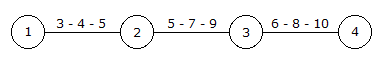
\includegraphics{../data_img/construction-planning-and-management_1525416187-17.png}
}
\\\begin{enumerate*}[itemjoin=\qquad, label=\Alph*.]
\item{1-2 is 4}
\item{2-3 is 7}
\item{3-4 is 8}
\item{All the above}
\end{enumerate*}
\item{Time and progress chart of a construction, is also known as}
\begin{enumerate}[label=\Alph*.]
\item{Bar chart}
\item{Gantt chart}
\item{Modified Mile stone chart}
\item{All the above}
\end{enumerate}
\item{The difference between the time avail-to do a job and the time required to do the job, is known as}
\\\begin{enumerate*}[itemjoin=\qquad, label=\Alph*.]
\item{Event}
\item{Float}
\item{Duration}
\item{Constraint}
\end{enumerate*}
\item{The Overall in-charge of an organization at the site responsible for the execution of the works, is}
\begin{enumerate}[label=\Alph*.]
\item{Executive Engineer}
\item{Engineer}
\item{Junior Engineer}
\item{Assistant Engineer}
\end{enumerate}
\item{For the supply of materials for concrete, form work reinforcing and placing of concrete, removal of form work and curing of concrete, number of bar(s) required on bar chart, is}
\\\begin{enumerate*}[itemjoin=\qquad, label=\Alph*.]
\item{1}
\item{2}
\item{3}
\item{4}
\end{enumerate*}
\item{Various activities of a project, are shown on bar charts by}
\begin{enumerate}[label=\Alph*.]
\item{Vertical lines}
\item{Horizontal lines}
\item{Dots}
\item{Crosses}
\end{enumerate}
\item{The main disadvantage of line organization, is}
\begin{enumerate}[label=\Alph*.]
\item{Rigid structure}
\item{Extraordinary delay in communications}
\item{Top level executions over work}
\item{All the above}
\end{enumerate}
\item{The main principle of an organization, is}
\begin{enumerate}[label=\Alph*.]
\item{Unity of command}
\item{Effective control at all levels}
\item{Delegation of authority}
\item{All the above}
\end{enumerate}
\item{A critical ratio scheduling}
\begin{enumerate}[label=\Alph*.]
\item{Determines the status of each activity}
\item{Adjusts automatically changes in activity progress}
\item{Is a dynamic system}
\item{None of these}
\end{enumerate}
\item{A golden rule for the procurement of construction stones, suggests}
\begin{enumerate}[label=\Alph*.]
\item{100\% at the site}
\item{67\% at the site and 33\% under procurement}
\item{50\% at the site and 50\% under procurement}
\item{33\% at the site and 67\% under procurement}
\end{enumerate}
\item{If a is the optimistic time, b is the pessimistic time and m is most likely time of an activity, the expected time of the activity, is}
\\\begin{enumerate*}[itemjoin=\qquad, label=\Alph*.]
\item{$ \frac{{{\text{a}} + {\text{m}} + {\text{b}}}}{6} $}
\item{$ \frac{{{\text{a}} + 2{\text{m}} + {\text{b}}}}{6} $}
\item{$ \frac{{{\text{a}} + 4{\text{m}} + {\text{b}}}}{6} $}
\item{$ \frac{{{\text{a}} + 5{\text{m}} + {\text{b}}}}{6} $}
\end{enumerate*}
\item{A four wheel truck or whose operating weight is 12000 kg is pulled along a road having a rising slope of 2\% at a uniform speed. Assume grade resistance factor = 10 kg/tonne. The tension in the tow cable is 720 kg. The rolling resistance of the road will be}
\\\begin{enumerate*}[itemjoin=\qquad, label=\Alph*.]
\item{20 kg/tonne}
\item{30 kg/tonne}
\item{40 kg/tonne}
\item{50 kg/tonne}
\end{enumerate*}
\item{A tractor whose weight is 20 tonnes has a drawbar pull of 2500 kg, when operated on a level road having a rolling resistance of 30 kg per tonne. If this tractor is operated on a level road having a rolling resistance of 40 kg per tonne, then the drawbar pull of the tractor will}
\begin{enumerate}[label=\Alph*.]
\item{Reduce by 200 kg}
\item{Increase by 200 kg}
\item{Increase by 250 kg}
\item{Reduce by 250 kg}
\end{enumerate}
\item{The time with which direct cost does not reduce with the increase in time is known as}
\begin{enumerate}[label=\Alph*.]
\item{Crash time}
\item{Normal time}
\item{Optimistic time}
\item{Standard time}
\end{enumerate}
\item{If the gross vehicle weight of a truck is 30 tonne and rolling resistance is 30 kg/tonne, then the tractive effort required to keep the truck moving at a uniform speed is}
\\\begin{enumerate*}[itemjoin=\qquad, label=\Alph*.]
\item{30 kg}
\item{300 kg}
\item{900 kg}
\item{1000 kg}
\end{enumerate*}
\item{For a given size of bucket, the ideal output of a dragline will be least in}
\begin{enumerate}[label=\Alph*.]
\item{Moist loam}
\item{Sand and gravel}
\item{Good common earth}
\item{Wet sticky clay}
\end{enumerate}
\item{Frederick W. Taylor introduced a system of working known as}
\begin{enumerate}[label=\Alph*.]
\item{Line organization}
\item{Line and staff organization}
\item{Functional organization}
\item{Effective organization}
\end{enumerate}
\item{For the execution of a project, a contractor is}
\\\begin{enumerate*}[itemjoin=\qquad, label=\Alph*.]
\item{A person}
\item{A firm}
\item{An agency}
\item{All the above}
\end{enumerate*}
\item{An earth moving equipment costs Rs. 5,00,000 and has an estimated life of 10 years and a salvage value of Rs. 50,000. What uniform annual amount must be set aside at the end of each of the 10 years for replacement if the interest rate is 8\% per annum and if the sinking fund factor at 8\% per annum interest rate for 10 years is 0.069?}
\\\begin{enumerate*}[itemjoin=\qquad, label=\Alph*.]
\item{Rs. 31050}
\item{Rs. 34500}
\item{Rs. 37950}
\item{Rs. 50000}
\end{enumerate*}
\item{Works costing less than Rs. 20,000 are treated as}
\\\begin{enumerate*}[itemjoin=\qquad, label=\Alph*.]
\item{Any project}
\item{Major projects}
\item{Minor projects}
\item{All the above}
\end{enumerate*}
\item{If the expected time for completion of a project is 10 days with a standard deviation of 2 days, the expected time of completion of the project with 99.9\% probability is}
\\\begin{enumerate*}[itemjoin=\qquad, label=\Alph*.]
\item{4 days}
\item{6 days}
\item{10 days}
\item{16 days}
\end{enumerate*}
\item{A dummy activity}
\begin{enumerate}[label=\Alph*.]
\item{Is artificially introduced}
\item{Is represented by a dotted line}
\item{Does not consume time}
\item{All the above}
\end{enumerate}
\item{A Milestone chart}
\begin{enumerate}[label=\Alph*.]
\item{Shows the interdependencies of various jobs}
\item{Depicts the delay of jobs, if any}
\item{Points outgoing ahead of schedule of jobs, if any}
\item{None of these}
\end{enumerate}
\item{Consider the following features/factors: \\
 1. Projects are of the non-repetitive type \\
 2. Time required need not be known \\
 3. Time required is known precisely \\
 4. Events have been established for planning \\
 5. Emphasis is given to activities of project \\
 PERT is preferred for planning because of}
\\\begin{enumerate*}[itemjoin=\qquad, label=\Alph*.]
\item{1, 2 and 4}
\item{3, 4 and 5}
\item{1, 3 and 4}
\item{1, 2 and 5}
\end{enumerate*}
\item{Consider the following statements: \\
 In the bar chart planning \\
 1. Interdependence of the operations cannot be portrayed. \\
 2. Progress of work can be measured. \\
 3. Spare time of the activities can be determined. \\
 4. Schedule cannot be updated.}
\begin{enumerate}[label=\Alph*.]
\item{1, 2 and 3 are correct}
\item{1 and 4 are correct}
\item{2, 3 and 4 are correct}
\item{1, 2 and 4 are correct}
\end{enumerate}
\item{Batching refers to}
\begin{enumerate}[label=\Alph*.]
\item{Controlling the total quantity at each batch}
\item{Weighing accurately, the quantity of each material for a job before mixing}
\item{Controlling the quantity of each material into each batch}
\item{Adjusting the water to be added in each batch according to the moisture content of the materials being mixed in the batch}
\end{enumerate}
\item{Military organization is known as}
\begin{enumerate}[label=\Alph*.]
\item{Line organization}
\item{Line and staff organization}
\item{Functional organization}
\item{None of these}
\end{enumerate}
\item{Critical path lies along the activities having total float}
\\\begin{enumerate*}[itemjoin=\qquad, label=\Alph*.]
\item{Positive}
\item{Negative}
\item{Zero}
\item{Same}
\end{enumerate*}
\item{An excavator costs Rs. 20,00,000 and has an estimated life of 8 years. It has no salvage value at the end of 8 years. The book value of the excavator at the end of 3 years using general double declining balance method is}
\\\begin{enumerate*}[itemjoin=\qquad, label=\Alph*.]
\item{Rs. 8,43,750}
\item{Rs. 8,75,000}
\item{Rs. 10,50,000}
\item{Rs. 11,56,250}
\end{enumerate*}
\item{Slack time refers to}
\begin{enumerate}[label=\Alph*.]
\item{An activity}
\item{An event}
\item{Both event and activity}
\item{None of the above}
\end{enumerate}
\item{The most suitable type of equipment for compaction of cohesive soils is}
\begin{enumerate}[label=\Alph*.]
\item{Smooth-wheeled rollers}
\item{Vibratory rollers}
\item{Sheep foot rollers}
\item{Tampers}
\end{enumerate}
\item{The most popular type of organization used for Civil Engineering Constructions, is}
\begin{enumerate}[label=\Alph*.]
\item{Line organization}
\item{Line and staff organization}
\item{Functional organization}
\item{Effective organization}
\end{enumerate}
\item{CPM is}
\begin{enumerate}[label=\Alph*.]
\item{Synthesising in concepts}
\item{Is built of activities oriented programme}
\item{Is based on time estimate}
\item{All the above}
\end{enumerate}
\item{In time-cost optimization of a project, crashing is done.}
\begin{enumerate}[label=\Alph*.]
\item{On all the activities}
\item{On all the activities lying on the critical path}
\item{Only on activities lying on the original critical path and having flatter cost slopes}
\item{On original critical activities and those that become critical at any stage of crashing in the order of ascending cost slope}
\end{enumerate}
\item{Critical path}
\begin{enumerate}[label=\Alph*.]
\item{Is always longest}
\item{Is always shortest}
\item{May be longest}
\item{May be shortest}
\end{enumerate}
\item{Earliest finish of an activity is always}
\begin{enumerate}[label=\Alph*.]
\item{Greater than earliest event time of the following node}
\item{Less than earliest event time of the following node}
\item{Less than or equal to earliest event time of the following node}
\item{Greater than or equal to earliest event time of the following node}
\end{enumerate}
\item{Latest start of an activity is always}
\begin{enumerate}[label=\Alph*.]
\item{greater than or equal to latest event time of preceding node}
\item{less than or equal to latest event time of preceding node}
\item{equal to latest event time of preceding node}
\item{less than latest event time of preceding node}
\end{enumerate}
\item{The rated loads of lifting cranes, as percentage of tipping load at specified radius, for crawler-mounted and pneumatic tyre-mounted machines would be respectively}
\\\begin{enumerate*}[itemjoin=\qquad, label=\Alph*.]
\item{80 and 90}
\item{90 and 80}
\item{85 and 75}
\item{75 and 83}
\end{enumerate*}
\item{In the time-cost optimisation, using CPM method for network analysis, the crashing of the activities along the critical path is done starting with the activity having}
\begin{enumerate}[label=\Alph*.]
\item{Longest duration}
\item{Highest cost slope}
\item{Least cost slope}
\item{Shortest duration}
\end{enumerate}
\item{A machine costs Rs. 20000 and its useful life is 8 years. The money is borrowed at 8\% interest per annum. The capital recovery factor at 8\% interest per annum for 8 years is 0.174. The annual equipment cost of the machine will be}
\\\begin{enumerate*}[itemjoin=\qquad, label=\Alph*.]
\item{Rs. 1740}
\item{Rs. 3480}
\item{Rs. 5220}
\item{Rs. 6960}
\end{enumerate*}
\item{Consider the following statements for a power shovel: \\
 (i) Output can be increased by reducing the angle of swing for a given depth of cut. \\
 (ii) For a given angle of swing, output will be maximum at optimum depth of cut. \\
 (iii) Output can be increased by keeping the depth of cut less than optimum depth. \\
 (iv) Output can be increased by increasing the size of shovel.}
\begin{enumerate}[label=\Alph*.]
\item{(ii), (iii) and (iv) are correct}
\item{(i), (ii) and (iv) are correct}
\item{(i), (iii) and (iv) are correct}
\item{(i) and (iv) are correct}
\end{enumerate}
\item{For which of the following materials, the output of power shovels for a fixed shovel size will be maximum}
\begin{enumerate}[label=\Alph*.]
\item{Moist loam}
\item{Good common earth}
\item{Well blasted rock}
\item{Wet sticky clay}
\end{enumerate}
\item{The original cost of an equipment is Rs.10,000. Its salvage value at the end of its total useful life of five years is Rs. 1,000. Its book value at the end of two years of its useful life (as per straight line method of evaluation of depreciation) will be}
\\\begin{enumerate*}[itemjoin=\qquad, label=\Alph*.]
\item{Rs. 8,800}
\item{Rs. 7,600}
\item{Rs. 6,400}
\item{Rs. 5,000}
\end{enumerate*}
\item{Crash project duration is obtained by summing the}
\begin{enumerate}[label=\Alph*.]
\item{Normal durations for all the activities}
\item{Crash durations for all activities}
\item{Crash durations for all the activities along the critical path obtained by taking into account the normal duration for all the activities}
\item{Crash durations for all the activities along the critical path obtained by taking into account the crash duration for all the activities}
\end{enumerate}
\item{Mile Stone charts were invented in the year of}
\\\begin{enumerate*}[itemjoin=\qquad, label=\Alph*.]
\item{1910}
\item{1920}
\item{1930}
\item{1940}
\end{enumerate*}
\item{Which one of the following represents an activity?}
\begin{enumerate}[label=\Alph*.]
\item{Excavation for foundation}
\item{Curing of concrete}
\item{Setting of question paper}
\item{All the above}
\end{enumerate}
\item{The part of a derrick crane include \\
 (i) Mast \\
 (ii) Boom \\
 (iii) Bull wheel \\
 (iv) Jack \\
 which of these statements are correct?}
\begin{enumerate}[label=\Alph*.]
\item{(i), (ii) and (iv) are correct}
\item{(ii), (iii) and (iv) are correct}
\item{(i), (iii) and (iv) are correct}
\item{(i), (ii) and (iii) are correct}
\end{enumerate}
\item{For excavating utility trenches with precise control of depth, the excavation equipment used is}
\begin{enumerate}[label=\Alph*.]
\item{Hoe}
\item{Shovel}
\item{Dragline}
\item{None of the above}
\end{enumerate}
\item{Which of the following surfaces will give highest rolling resistance for a rubber tyred vehicle?}
\\\begin{enumerate*}[itemjoin=\qquad, label=\Alph*.]
\item{Concrete}
\item{Loose sand}
\item{Asphalt}
\item{Firm earth}
\end{enumerate*}
\item{Power stations are generally treated as}
\begin{enumerate}[label=\Alph*.]
\item{Light construction}
\item{Heavy construction}
\item{Industrial construction}
\item{Electrical construction}
\end{enumerate}
\item{If the optimistic time, most likely time and pessimistic time for activity A are 4, 6 and 8 respectively and for activity B are 5, 5.5 and 9 respectively, then}
\begin{enumerate}[label=\Alph*.]
\item{expected time of activity A is greater than the expected time of activity B}
\item{expected time of activity B is greater than the expected time of activity A}
\item{expected time of both activities A and B are same}
\item{none of the above}
\end{enumerate}
\item{Which of the following is a weakness of bar chart?}
\begin{enumerate}[label=\Alph*.]
\item{Interdependencies of activities}
\item{Project progress}
\item{Uncertainties}
\item{All of the above}
\end{enumerate}
\item{For completion of a project, the critical path of the network represents}
\\\begin{enumerate*}[itemjoin=\qquad, label=\Alph*.]
\item{Minimum time}
\item{Maximum time}
\item{Maximum cost}
\item{Minimum cost}
\end{enumerate*}
\item{A machine is purchased for Rs. 10,000,00 and has an estimated life of 10 years. The salvage value at the end of 10 years is Rs. 1,50,000. The book value of the machine at the end of 5 years using general straight line method of evaluation of depreciation is}
\\\begin{enumerate*}[itemjoin=\qquad, label=\Alph*.]
\item{Rs. 4,75,000}
\item{Rs. 5,75,000}
\item{Rs. 6,50,000}
\item{Rs. 8,50,000}
\end{enumerate*}
\item{Which of the following excavators is most suitable for digging under water?}
\\\begin{enumerate*}[itemjoin=\qquad, label=\Alph*.]
\item{Drag line}
\item{Hoe}
\item{Clam shell}
\item{Dipper shovel}
\end{enumerate*}
\item{Rolling resistance of a wheel depends upon \\
 (i) Vehicle load \\
 (ii) Grade \\
 (iii) Ground conditions}
\begin{enumerate}[label=\Alph*.]
\item{Only (i) is correct}
\item{(i) and (ii) are correct}
\item{(i) and (iii) are correct}
\item{(ii) and (iii) are correct}
\end{enumerate}
\item{Residential buildings are treated as}
\begin{enumerate}[label=\Alph*.]
\item{Light construction}
\item{Heavy construction}
\item{Industrial construction}
\item{Private construction}
\end{enumerate}
\item{Output of a bulldozer is \\
 (i) Increased if drawbar HP of the tractor is increased for a given hauling distance \\
 (ii) Decreased if drawbar HP of the tractor is increased for a given hauling distance \\
 (iii) Increased if the hauling distance is increased for a given drawbar HP of the tractor \\
 (iv) Decreased if the hauling distance is increased for a given drawbar HP of the tractor}
\begin{enumerate}[label=\Alph*.]
\item{(i) and (iii) are correct}
\item{(i) and (iv) are correct}
\item{(ii) and (iii) are correct}
\item{(ii) and (iv) are correct}
\end{enumerate}
\item{The critical activity has}
\\\begin{enumerate*}[itemjoin=\qquad, label=\Alph*.]
\item{Maximum float}
\item{Minimum float}
\item{Zero float}
\item{None of these}
\end{enumerate*}
\item{The object of technical planning, is}
\begin{enumerate}[label=\Alph*.]
\item{Preparation of specifications}
\item{Preparation of estimates}
\item{Initiating the procurement action of resources}
\item{All the above}
\end{enumerate}
\item{Total float for any activity is defined as the difference between}
\begin{enumerate}[label=\Alph*.]
\item{Its latest finish time and earliest start time for its successor activity}
\item{Its latest start time and earliest start time}
\item{Its latest start time and earliest finish time}
\item{Its earliest finish time and earliest start time for its successor activity}
\end{enumerate}
\end{enumerate}
\textbf{Answer Key}
\begin{tabular}{ | c | c c c c c c c c c c | }
\hline
 & 1 & 2 & 3 & 4 & 5 & 6 & 7 & 8 & 9 & 0 \\
\hline
0 & C & E & D & C & A & C & C & A & B & D \\
10 & D & B & B & A & B & D & D & D & B & C \\
20 & C & A & B & C & D & C & D & A & C & D \\
30 & D & D & A & B & C & A & C & A & B & C \\
40 & A & D & D & A & C & A & D & C & B & B \\
50 & A & C & D & D & D & D & A & B & C & C \\
60 & D & A & B & A & C & A & B & C & D & B \\
\hline
\end{tabular}
\clearpage
\subsection*{Section 2}
\begin{enumerate}
\item{Interfering float is the difference between}
\begin{enumerate}[label=\Alph*.]
\item{Total float and free float}
\item{Total float and independent float}
\item{Free float and independent float}
\item{None of the above}
\end{enumerate}
\item{Free float for any activity is defined as the difference between}
\begin{enumerate}[label=\Alph*.]
\item{its earliest finish time and earliest start time for its successor activity}
\item{its latest start time and earliest start time}
\item{its latest finish time and earliest start time for its successor activity}
\item{its earliest finish time and latest start time for its successor activity}
\end{enumerate}
\item{Assertion A: For a given depth of cut, the output of a power shovel can be increased by decreasing the angle of swing. \\
Reason R: If the angle of swing is decreased, the cycle time will be decreased.}
\begin{enumerate}[label=\Alph*.]
\item{Both A and R is true and R is the correct explanation of A}
\item{Both A and R is true but R is not the correct explanation of A}
\item{A is true but R is false}
\item{A is false but R is true}
\end{enumerate}
\item{Consider the following statements:  \\
 In the critical path method of construction planning, Free Float can be. \\
 1. Greater than Total Float. \\
 2. Greater than Independent Float \\
 3. Equal to Total Float. \\
 4. Less than Independent Float}
\begin{enumerate}[label=\Alph*.]
\item{1 and 4 are correct}
\item{2 and 3 are correct}
\item{1 and 4 are correct}
\item{1 and 2 are correct}
\end{enumerate}
\item{Updating may result in}
\begin{enumerate}[label=\Alph*.]
\item{Change of critical path}
\item{Decrease of project completion time}
\item{Increase of project completion time}
\item{All of the above}
\end{enumerate}
\item{The first method invented for planning projects, was}
\begin{enumerate}[label=\Alph*.]
\item{Bar chart method}
\item{Milestone chart}
\item{Critical path method (CPM)}
\item{Programme Evaluation and Review Technique (PERT)}
\end{enumerate}
\item{A contractor has two options; (l) : Invest his money in project A or (II) : Invest his money in project B. If he decides to invest in A, for every rupee invested, he is assured of doubling his money in ten years. If he decides to invest in B, he is assured of making his money 1.5 times in 5 years. If the contractor values his money at 10\% interest rate, he
}
\begin{enumerate}[label=\Alph*.]
\item{Should invest in neither of the two projects}
\item{Could invest in either of the two projects}
\item{Should invest in project A}
\item{Should invest in project B}
\end{enumerate}
\item{Free float is mainly used to}
\begin{enumerate}[label=\Alph*.]
\item{Identify the activities which can be delayed without affecting the total float of preceding activity}
\item{Identify the activities, which can be delayed without affecting the total float of succeeding activity}
\item{Establish priorities}
\item{Identify the activities which can be delayed without affecting the total float of either the preceding or succeeding activities}
\end{enumerate}
\item{The time by which a particular activity can be delayed without affecting the preceding and succeeding activities is known as}
\begin{enumerate}[label=\Alph*.]
\item{Total float}
\item{Free float}
\item{Interfering float}
\item{Independent float}
\end{enumerate}
\item{Preliminary project report for a road project must contain}
\begin{enumerate}[label=\Alph*.]
\item{The detailed estimated cost based on detailed design}
\item{The several alternatives of the project that have been considered}
\item{The soil survey, traffic survey, concept design and approximate cost}
\item{The contract documents for inviting tenders}
\end{enumerate}
\item{Consider the following operations: \\
 1. Drilling \\
 2. Blasting \\
 3. Mucking \\
 4. Placing steel \\
 5. Placing concrete \\
 The correct sequence of these operations in tunnel construction is}
\\\begin{enumerate*}[itemjoin=\qquad, label=\Alph*.]
\item{1, 2, 4, 3, 5}
\item{1, 3, 2, 4, 5}
\item{1, 2, 3, 4, 5}
\item{1, 3, 4, 2, 5}
\end{enumerate*}
\item{The salient feature of functional organization is}
\begin{enumerate}[label=\Alph*.]
\item{Strict adherence to specifications}
\item{Separation of planning and design part}
\item{Each individual maintains functional efficiency}
\item{All the above}
\end{enumerate}
\item{The time corresponding to minimum total project cost is}
\begin{enumerate}[label=\Alph*.]
\item{Crash time}
\item{Normal time}
\item{Optimistic time}
\item{Between normal time and crash time}
\end{enumerate}
\item{The process of incorporating changes and rescheduling or replanning is called}
\begin{enumerate}[label=\Alph*.]
\item{Resource levelling}
\item{Resource smoothening}
\item{Updating}
\item{Critical path scheduling}
\end{enumerate}
\item{If D is the duration, ES and EF are the earliest start and finish, LS and LF are latest start and latest finish time, then the following relation holds good}
\\\begin{enumerate*}[itemjoin=\qquad, label=\Alph*.]
\item{EF = ES + D}
\item{LS = LF - D}
\item{LF = LS + D}
\item{All the above}
\end{enumerate*}
\item{The artificial activity which indicates that an activity following it, cannot be started unless the preceding activity is complete, is known as}
\\\begin{enumerate*}[itemjoin=\qquad, label=\Alph*.]
\item{Event}
\item{Free float}
\item{Dummy}
\item{Constraint}
\end{enumerate*}
\item{The independent float affects only}
\begin{enumerate}[label=\Alph*.]
\item{Preceding activities}
\item{Succeeding activities}
\item{The particular activity involved}
\item{None of the above}
\end{enumerate}
\item{PERT analysis is based on}
\begin{enumerate}[label=\Alph*.]
\item{Optimistic time}
\item{Pessimistic time}
\item{Most likely time}
\item{All the above}
\end{enumerate}
\item{Pick up the correct statement from the following with regards to C.P.M. network analysis of projects}
\begin{enumerate}[label=\Alph*.]
\item{The latest occurrence time of the node of which the activity arrow terminates minus the duration of the activity, is called latest start time}
\item{The latest occurrence time for the node at which the activity arrow terminates, is called latest finish time}
\item{Earliest occurrence time of the event from which the activity arrow' originates, is called earliest start time of the activity}
\item{All the above}
\end{enumerate}
\item{A CPM family includes}
\begin{enumerate}[label=\Alph*.]
\item{CPA (Critical Path Analysis)}
\item{CPP (Critical Path Plotted)}
\item{MCE (Minimum Cost Expenditure)}
\item{All the above}
\end{enumerate}
\item{PERT technique of network analysis is mainly useful for}
\begin{enumerate}[label=\Alph*.]
\item{Small projects}
\item{Large and complex projects}
\item{Research and development projects}
\item{Deterministic activities}
\end{enumerate}
\item{In India, are prefabricated components costlier than those of traditional cast-in-situ items that the prefabricated components replace?}
\begin{enumerate}[label=\Alph*.]
\item{Yes, because of heavier overheads and handling cost}
\item{Yes, because of the very high order of quality control for the factory made components}
\item{No, because of repetitive manufacture of a number of elements}
\item{No, because of savings in site labour}
\end{enumerate}
\item{What estimate would you give for the variance in above problem ?}
\\\begin{enumerate*}[itemjoin=\qquad, label=\Alph*.]
\item{81}
\item{54}
\item{36}
\item{9}
\end{enumerate*}
\item{Mobilization advance up to 10\% of the cost of work is given to a contractor}
\begin{enumerate}[label=\Alph*.]
\item{On commencement of work at site for payment of loan taken by him}
\item{For the purchase of construction materials}
\item{For the payment of advances to labour and other staff}
\item{For all activities required to start the work at site on finalization of the contract document}
\end{enumerate}
\item{Which of the following is not a PERT event?}
\begin{enumerate}[label=\Alph*.]
\item{Site investigation started}
\item{Sessional work completed}
\item{Bus starts from Jaipur}
\item{Class is being attended}
\end{enumerate}
\item{During the construction period, price variation clause in contracts caters to}
\begin{enumerate}[label=\Alph*.]
\item{Increase in rates of only important materials}
\item{Variation in cost in materials element, labour element and petrol-oil-lubricant element}
\item{Variation in total cost of the project on an ad hoc basis}
\item{Rate of inflation}
\end{enumerate}
\item{In PERT analysis, the time estimates of activities and probability of their occurrence follow}
\begin{enumerate}[label=\Alph*.]
\item{Normal distribution curve}
\item{Poisson's distribution curve}
\item{Beta distribution curve}
\item{None of the above}
\end{enumerate}
\item{At a work site, statistical quality control of concrete means}
\begin{enumerate}[label=\Alph*.]
\item{Measurement of risks to eliminate failures}
\item{Applying the theory' of probability to sample testing or inspection}
\item{Reduction in wastage of inspection costs}
\item{Reduction in costs for the removal of defects}
\end{enumerate}
\item{Pick up the incorrect statement from the following:}
\begin{enumerate}[label=\Alph*.]
\item{An activity of a project is denoted by an arrow on the net work}
\item{The tail of the arrow indicates the start of the activity}
\item{The head of the arrow indicates the end of the activity}
\item{The arrows are drawn to scale from left to right}
\end{enumerate}
\item{Pick up the PERT event from the following:}
\begin{enumerate}[label=\Alph*.]
\item{Digging of foundation started}
\item{Digging of foundation completed}
\item{Laying of concrete started}
\item{All the above}
\end{enumerate}
\item{Pick up the correct statement from the following:}
\begin{enumerate}[label=\Alph*.]
\item{Earliest expected time is denoted by TE}
\item{Latest occurrence time is denoted by TL}
\item{Contractual obligation time is denoted by Ts}
\item{All the above}
\end{enumerate}
\item{Pick up the correct statement from the following:}
\begin{enumerate}[label=\Alph*.]
\item{Forward pass is used for calculating earliest expected time}
\item{Backward pass is used for calculating the latest occurrence time}
\item{Maximum value of earliest expected time is used if there is more than one value of any event}
\item{All the above}
\end{enumerate}
\item{Pick up the correct statement from the following:}
\begin{enumerate}[label=\Alph*.]
\item{Optimistic time estimate refers to activities}
\item{Pessimistic time estimate refers to activities}
\item{Most likely time estimate refers to activities}
\item{All the above}
\end{enumerate}
\item{Pick up the correct statement from the following:}
\begin{enumerate}[label=\Alph*.]
\item{Programme Evaluation and Review Technique, is event oriented}
\item{Programme Evaluation and Review Technique is not event oriented}
\item{Critical Path Method is event oriented}
\item{Critical Path Method is not event oriented}
\end{enumerate}
\item{Pick up the incorrect statement from the following:}
\begin{enumerate}[label=\Alph*.]
\item{The activity is the time consuming part of a project}
\item{The beginning and end of a job, are called events}
\item{The activity which consumes maximum time, is called a node}
\item{Logically and sequentially connected activities and events form a network}
\end{enumerate}
\item{Pick up the incorrect statement from the following:}
\begin{enumerate}[label=\Alph*.]
\item{The difference between the earliest start time and latest finish time of any activity, is the maximum time available for the activity}
\item{The difference between the maximum time available for the job and actual time it consumes, is called total float}
\item{The difference between the latest start time and earliest start time of an activity, is called total float}
\item{None of these}
\end{enumerate}
\item{Pick up the correct statement from the following:}
\begin{enumerate}[label=\Alph*.]
\item{The difference of latest occurrence time and earliest expected time, is called slack}
\item{The activities connecting the events having zero slack, lie on the critical path}
\item{The critical path consumes the maximum time}
\item{All the above}
\end{enumerate}
\item{Pick up the correct statement from the following:}
\begin{enumerate}[label=\Alph*.]
\item{The duration between the earliest start time of the preceding event and latest finish time of the succeeding event, is called 'float'}
\item{The duration of time by which an activity can be delayed without affecting the succeeding activity, is called free float}
\item{The difference between total float and free float, is called interfering float}
\item{All the above}
\end{enumerate}
\item{Pick up the correct statement from the following:}
\begin{enumerate}[label=\Alph*.]
\item{The float may be positive, zero or negative}
\item{If the float is positive and the activity is delayed by a period equal to its total float, the completion of project is not delayed}
\item{If the float of an activity is negative, delay in its performance is bound to delay the completion of project}
\item{All the above}
\end{enumerate}
\item{Pick up the incorrect statement from the following:}
\begin{enumerate}[label=\Alph*.]
\item{The various functions under each activity, are shown by one bar on Bar Charts}
\item{Bar chart establishes the interdependency of one event on another}
\item{Only approximate percentage of the completed work is reported}
\item{None of these}
\end{enumerate}
\item{Select the correct statement.}
\begin{enumerate}[label=\Alph*.]
\item{Activity arrows in a CPM network are drawn to scale}
\item{The tail of an arrow represents the finish of an activity}
\item{Arrow bead represents the start of an activity}
\item{None of the above}
\end{enumerate}
\item{Select the incorrect statement.}
\begin{enumerate}[label=\Alph*.]
\item{Earliest start of an activity is the early event time of the node it leaves}
\item{Latest finish of an activity is the late event time of the node it enters}
\item{Latest start of an activity is its latest finish minus its duration}
\item{None of the above}
\end{enumerate}
\item{Select the incorrect statement.}
\begin{enumerate}[label=\Alph*.]
\item{Start float and finish float are always equal}
\item{Total float can be either start float or finish float}
\item{Start float and finish float need not be equal}
\item{Start float and finish float are the differences between activity times and not event times}
\end{enumerate}
\item{Select the incorrect statement.}
\begin{enumerate}[label=\Alph*.]
\item{A critical path always begins at the very first event.}
\item{A critical path always terminates at the last event.}
\item{Critical activities control the project duration.}
\item{Critical activity is the one for which free float is zero.}
\end{enumerate}
\item{Wheeled tractors are replacing crawler tractors because \\
 1. Wheeled tractors travel faster. \\
 2. Crawler tractors are more expensive. \\
 3. Track parts of a crawler wear out quickly. \\
 4. Crawler tractors have stick control. \\
 of following statements
}
\begin{enumerate}[label=\Alph*.]
\item{1, 3 and 4 are correct}
\item{2, 3 and 4 are correct}
\item{1, 2 and 3 are correct}
\item{1, 2 and 4 are correct}
\end{enumerate}
\item{The maximum rimpull in the first gear of a tractor while towing a load is 6300 kg. The tractor weighs 12.5 tonnes and is operating along a 2 percent upgrade and the rolling resistance is 45 kg/tonne. Pull available for towing the load is}
\\\begin{enumerate*}[itemjoin=\qquad, label=\Alph*.]
\item{3425 kg}
\item{5515 kg}
\item{4350 kg}
\item{2975 kg}
\end{enumerate*}
\item{The basic action involved in sheep foot rolling is}
\\\begin{enumerate*}[itemjoin=\qquad, label=\Alph*.]
\item{Kneading}
\item{Pressing}
\item{Tamping}
\item{Vibration}
\end{enumerate*}
\item{If the expected time of completion of a project is 60 weeks with a standard deviation of 5 weeks, the probability of completing the project in 50 weeks and 65 weeks respectively will be}
\begin{enumerate}[label=\Alph*.]
\item{2.3\% and 84.1\%}
\item{97.7\% and 84.1\%}
\item{97.7 \% and 15.9\%}
\item{15.9\% and 97.7\%}
\end{enumerate}
\item{The constraints in case of resource smoothening operation would be}
\begin{enumerate}[label=\Alph*.]
\item{Resources}
\item{Project duration time}
\item{Both resources and project duration time}
\item{None of the above}
\end{enumerate}
\item{PERT is}
\begin{enumerate}[label=\Alph*.]
\item{An analytic in concept}
\item{Limited of event oriented diagrams}
\item{Used for research and development projects}
\item{All the above}
\end{enumerate}
\item{While scheduling a project by C.P.M.}
\begin{enumerate}[label=\Alph*.]
\item{A project is divided into various activities}
\item{Required time for each activity is established}
\item{Net work is drawn by connecting the activities and the events}
\item{All the above}
\end{enumerate}
\item{Final technical authority of a project lies with}
\begin{enumerate}[label=\Alph*.]
\item{Assistant Engineer}
\item{Executive Engineer}
\item{Superintending Engineer}
\item{Chief Engineer}
\end{enumerate}
\item{The technique for establishing and maintaining priorities among the various jobs of a project, is known}
\begin{enumerate}[label=\Alph*.]
\item{Event flow scheduling technique}
\item{Critical ratio scheduling}
\item{Slotting technique for scheduling}
\item{Short interval scheduling}
\end{enumerate}
\item{If the total float and duration of an activity are 5 and 10 days respectively, the particular activity can be}
\begin{enumerate}[label=\Alph*.]
\item{Started 5 days later}
\item{Completed 5 days later}
\item{Performed at slower rate in 15 days}
\item{All the above}
\end{enumerate}
\item{Optimistic time, most likely time and pessimistic times for the activities of a network in the given figure are written above their arrows. If the contractual obligation time for the project is 75, the latest occurrence time for the event 2, is \\

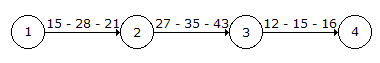
\includegraphics{../data_img/construction-planning-and-management_1525416235-18.png}
}
\\\begin{enumerate*}[itemjoin=\qquad, label=\Alph*.]
\item{20}
\item{25}
\item{35}
\item{15}
\end{enumerate*}
\item{The three time estimates for the activities of the network shown in the given figure are shown above their arrows. The earliest expected time for the event 4, is \\
 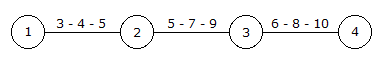
\includegraphics{../data_img/construction-planning-and-management_1525416269-17.png}
}
\\\begin{enumerate*}[itemjoin=\qquad, label=\Alph*.]
\item{19}
\item{14}
\item{24}
\item{None of these}
\end{enumerate*}
\item{Which one of the following surfaces will give highest coefficient of traction while using crawler track tractors?}
\\\begin{enumerate*}[itemjoin=\qquad, label=\Alph*.]
\item{Ice}
\item{Concrete}
\item{Loose sand}
\item{Earth}
\end{enumerate*}
\item{Which one of the following represents an event?}
\begin{enumerate}[label=\Alph*.]
\item{Concrete cured}
\item{Fixing of door}
\item{Plastering of walls}
\item{Selecting sites}
\end{enumerate}
\item{The reduction in project time normally results in}
\begin{enumerate}[label=\Alph*.]
\item{Decreasing the direct cost and increasing indirect cost}
\item{Increasing the direct cost and decreasing the indirect cost}
\item{Increasing the direct cost and indirect cost both}
\item{Decreasing the direct cost and indirect cost both}
\end{enumerate}
\item{In the given figure, the network of a project represents \\

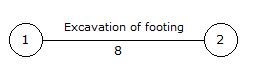
\includegraphics{../data_img/construction-planning-and-management_1525416299-19.png}
}
\begin{enumerate}[label=\Alph*.]
\item{Activity of an excavation of a footing}
\item{Activity of an excavation which starts at event No. 1 and ends at even No. 2}
\item{Activity of excavation which takes 8 units of time}
\item{None of these}
\end{enumerate}
\item{Which of the following earth moving machines has the shortest cycle time?}
\\\begin{enumerate*}[itemjoin=\qquad, label=\Alph*.]
\item{Drag line}
\item{Hoe}
\item{Clam shell}
\item{Dipper shovel}
\end{enumerate*}
\item{A tractor shovel has a purchase price of Rs. 4.7 lacs and could save the organization an amount of rupees one lac per year on operating costs. The salvage value after the amortization period is 10\% of the purchase price. The capital recovery period will be}
\\\begin{enumerate*}[itemjoin=\qquad, label=\Alph*.]
\item{3.7 years}
\item{4.23 years}
\item{5 years}
\item{7.87 years}
\end{enumerate*}
\item{Completion of an activity on CPM network diagram, is generally known}
\\\begin{enumerate*}[itemjoin=\qquad, label=\Alph*.]
\item{Event}
\item{Node}
\item{Connector}
\item{All the above}
\end{enumerate*}
\item{Grader is used mainly for}
\begin{enumerate}[label=\Alph*.]
\item{Trimming and finishing}
\item{Shaping and trimming}
\item{Finishing and shaping}
\item{Finishing, shaping and trimming}
\end{enumerate}
\item{Consider the following activities in a building construction: \\
 1. Concreting of roof slabs \\
 2. Brick-jelly lime concrete terracing \\
 3. Erection of form work for slab \\
 4. Construction of parapet wall in terrace \\
 The correct sequence of these activities is
}
\\\begin{enumerate*}[itemjoin=\qquad, label=\Alph*.]
\item{1, 3, 2, 4}
\item{3, 1, 4, 2}
\item{3, 1, 2, 4}
\item{1, 3, 4, 2}
\end{enumerate*}
\item{Site order book is used for recording}
\begin{enumerate}[label=\Alph*.]
\item{Instructions by the executive engineers}
\item{Construction measurements}
\item{Issue of store equipments}
\item{Names of the casual labour}
\end{enumerate}
\item{Which of the following does not represent an activity?}
\begin{enumerate}[label=\Alph*.]
\item{Site located}
\item{Foundation is being dug}
\item{The office area is being cleaned}
\item{The invitations are being sent}
\end{enumerate}
\item{Sinking fund is}
\begin{enumerate}[label=\Alph*.]
\item{The fund for rebuilding a structure when its economic life is over}
\item{Raised to meet maintenance costs}
\item{The total sum to be paid to the municipal authorities by the tenants}
\item{A part of the money kept in reserve for providing additional structures and structural modifications}
\end{enumerate}
\item{Sensitivity analysis is a study of}
\begin{enumerate}[label=\Alph*.]
\item{Comparison of profit and loss}
\item{Comparison of assets and liabilities}
\item{Change in output due to change in input}
\item{Economics of cost and benefits of the project}
\end{enumerate}
\item{In resources levelling}
\begin{enumerate}[label=\Alph*.]
\item{Total duration of project is reduced}
\item{Total duration of project is increased}
\item{Uniform demand of resources is achieved}
\item{Cost of project is controlled}
\end{enumerate}
\end{enumerate}
\textbf{Answer Key}
\begin{tabular}{ | c | c c c c c c c c c c | }
\hline
 & 1 & 2 & 3 & 4 & 5 & 6 & 7 & 8 & 9 & 0 \\
\hline
0 & A & A & A & B & D & A & A & B & D & C \\
10 & C & D & D & C & D & C & C & D & D & D \\
20 & C & C & A & D & D & B & C & B & D & D \\
30 & D & D & D & A & C & D & D & D & D & B \\
40 & D & D & C & D & C & B & A & A & B & D \\
50 & D & D & B & D & B & A & D & A & B & C \\
60 & D & B & D & D & C & A & A & A & C & C \\
\hline
\end{tabular}
\clearpage
\subsection*{Section 3}
\begin{enumerate}
\item{Frequency distribution curves}
\begin{enumerate}[label=\Alph*.]
\item{Having a single lump, are called uninodal curves}
\item{If symmetrical, are called normal curves}
\item{If not symmetrical, are called skew curves}
\item{All the above}
\end{enumerate}
\item{Economic saving of time results by crashing}
\begin{enumerate}[label=\Alph*.]
\item{Cheapest critical activity}
\item{Cheapest noncritical activity}
\item{Costliest critical activity}
\item{Costliest noncritical activity}
\end{enumerate}
\item{If the output of a drag-line for 90$^\circ$ angle of swing at optimum depth of cut is X, then the output for 120$^\circ$ angle of swing at 120\% of optimum depth of cut will be
}
\begin{enumerate}[label=\Alph*.]
\item{Equal to X}
\item{More than X}
\item{Less than X}
\item{Any of the above}
\end{enumerate}
\item{A wheeled tractor hauling unit is working on firm earth. The total loaded weight distribution of this unit is: \\
 Drive wheels: 25000 kg \\
 Scraper wheels: 10000 kg \\
If the coefficient of traction for wheeled tractor on firm earth is 0.5, the rimpull which this tractor can exert without slipping is}
\\\begin{enumerate*}[itemjoin=\qquad, label=\Alph*.]
\item{10000 kg}
\item{12500 kg}
\item{22500 kg}
\item{5000 kg}
\end{enumerate*}
\item{Critical path method}
\begin{enumerate}[label=\Alph*.]
\item{Is an improvement upon bar chart method}
\item{Provides a realistic approach to daily problems}
\item{Avoids delays which are very common in bar charts}
\item{All the above}
\end{enumerate}
\item{The time by which activity completion time can be delayed without affecting the start of succeeding activities, is known as}
\begin{enumerate}[label=\Alph*.]
\item{Duration}
\item{Total float}
\item{Free float}
\item{Interfering float}
\end{enumerate}
\item{If the scheduled completion time of a project is more than the earliest expected time for completion of the project, then the probability of completion of the project within the scheduled completion time will be}
\\\begin{enumerate*}[itemjoin=\qquad, label=\Alph*.]
\item{50 \%}
\item{Less than 50 \%}
\item{More than 50 \%}
\item{100 \%}
\end{enumerate*}
\item{The direct cost of a project with respect to normal time is}
\\\begin{enumerate*}[itemjoin=\qquad, label=\Alph*.]
\item{Minimum}
\item{Maximum}
\item{Zero}
\item{Infinite}
\end{enumerate*}
\item{Whenever an activity has zero total float, then}
\begin{enumerate}[label=\Alph*.]
\item{Free float of the activity must be zero but independent float need not be zero}
\item{Independent float must be zero but free float need not be zero}
\item{Free float and independent float both must be zero}
\item{Free float and independent float both need not be zero}
\end{enumerate}
\item{While filling the tender for any work, the contractor considers}
\begin{enumerate}[label=\Alph*.]
\item{Site survey}
\item{Availability of construction materials}
\item{Availability of labour}
\item{All the above}
\end{enumerate}
\item{Railway projects are treated as}
\begin{enumerate}[label=\Alph*.]
\item{Light construction}
\item{Heavy construction}
\item{Industrial construction}
\item{None of these}
\end{enumerate}
\item{If the excavation of earth is done manually then it costs Rs. 10 per cum. A machine can excavate at a fixed cost of Rs. 4000 plus a variable cost of Rs. 2 per cum. The quantity of earth for which the cost of excavation by machine will be equal to the cost of manual excavation is}
\\\begin{enumerate*}[itemjoin=\qquad, label=\Alph*.]
\item{500 cum}
\item{1000 cum}
\item{1500 cum}
\item{2000 cum}
\end{enumerate*}
\item{Construction team means}
\\\begin{enumerate*}[itemjoin=\qquad, label=\Alph*.]
\item{An engineer}
\item{An architect}
\item{An owner}
\item{All the above}
\end{enumerate*}
\item{Assertion (A): Activity 57 is critical. \\
Reason (R): Earliest finish time and latest finish time for events 57 are same}
\begin{enumerate}[label=\Alph*.]
\item{A is correct but R is not correct}
\item{R is correct but A is not correct}
\item{Both A and R is correct}
\item{Both A and R is incorrect}
\end{enumerate}
\item{The time which results in the least possible construction cost of an activity, is known as}
\\\begin{enumerate*}[itemjoin=\qquad, label=\Alph*.]
\item{Normal time}
\item{Slow time}
\item{Crash time}
\item{Standard time}
\end{enumerate*}
\item{The area under the Beta distribution curve is divided into two equal parts by}
\begin{enumerate}[label=\Alph*.]
\item{Most likely time}
\item{Optimistic time}
\item{Pessimistic time}
\item{Expected time}
\end{enumerate}
\item{The grade resistance factor for an earth moving machine can be obtained by multiplying grade percentage by a factor approximately equal to}
\\\begin{enumerate*}[itemjoin=\qquad, label=\Alph*.]
\item{2 kg/tonne}
\item{6 kg/tonne}
\item{9 kg/tonne}
\item{20 kg/tonne}
\end{enumerate*}
\item{Which one of the following is not an excavating and moving type of equipment?}
\\\begin{enumerate*}[itemjoin=\qquad, label=\Alph*.]
\item{Bulldozer}
\item{Clam shell}
\item{Scraper}
\item{Dump truck}
\end{enumerate*}
\end{enumerate}
\textbf{Answer Key}
\begin{tabular}{ | c | c c c c c c c c c c | }
\hline
 & 1 & 2 & 3 & 4 & 5 & 6 & 7 & 8 & 9 & 0 \\
\hline
0 & D & A & C & B & D & C & C & A & C & D \\
10 & B & A & D & A & B & D & C & D &   &   \\
\hline
\end{tabular}
\clearpage
\section{Engineering Economics}
\subsection*{Section 1}
\begin{enumerate}
\item{The CRF (ep) is also known as: [CRF(EP) - 8\% - 7], where}
\begin{enumerate}[label=\Alph*.]
\item{8\% is the rate of interest per year}
\item{Money is borrowed for n = 7 years}
\item{Both (A) and (B)}
\item{Neither (A) nor (B)}
\end{enumerate}
\item{A form of business organization in which a person conducts his business alone and entirely for his own profit, being solely responsible for all its activities and liabilities.}
\begin{enumerate}[label=\Alph*.]
\item{Sole proprietorship}
\item{Entrepreneurship}
\item{Partnership}
\item{Corporation}
\end{enumerate}
\item{A man loans P 187,400 from a bank with interest at 5\% compounded annually. He agrees to pay his obligations by paying 8 equal annual payments, the first being due at the end of 10 years. Find the annual payments.}
\\\begin{enumerate*}[itemjoin=\qquad, label=\Alph*.]
\item{P 43,600.10}
\item{P 43,489.47}
\item{P 43,263.91}
\item{P 43,763.20}
\end{enumerate*}
\item{Keeping in view, the feasibility order of magnitude, the preliminary, conceptual or budget estimates, are prepared by:}
\begin{enumerate}[label=\Alph*.]
\item{Architect/engineer}
\item{Construction manager}
\item{Owner himself/herself}
\item{Construction manager}
\end{enumerate}
\item{What is the reduction in the money value of capital asset is called?}
\begin{enumerate}[label=\Alph*.]
\item{Capital expenditure}
\item{Capital loss}
\item{Loss}
\item{Deficit}
\end{enumerate}
\item{What is the increase in the money value of a capital asset is called?}
\begin{enumerate}[label=\Alph*.]
\item{Profit}
\item{Capital gain}
\item{Capital expenditure}
\item{Capital stock}
\end{enumerate}
\item{A construction estimate is used}
\begin{enumerate}[label=\Alph*.]
\item{To judge tentatively or approximate value of the project}
\item{To produce a statement of the approximate cost}
\item{To decide an approximation of the value of the project and not the exact cost}
\item{None of these}
\end{enumerate}
\item{If P is principal amount, $$I$$ is the rate of interest per annum and n is the number of periods in years, the compound amount factor (CAF) is:
}
\\\begin{enumerate*}[itemjoin=\qquad, label=\Alph*.]
\item{$ {\left( {1 + I} \right)^{\text{n}}} $}
\item{$ {\left( {1 + I} \right)^{\frac{1}{{2{\text{n}}}}}} $}
\item{$ \sqrt {{\text{n}} + I}  $}
\item{None of these}
\end{enumerate*}
\item{If interest is paid more than once in a year, `i' is the rate of interest per year, `n' is the number of periods in years and `m' is a number of periods per years, compound amount factor (CAF) is:
}
\\\begin{enumerate*}[itemjoin=\qquad, label=\Alph*.]
\item{$ {\left( {1 + \frac{{\text{i}}}{{\text{m}}}} \right)^{\text{n}}} $}
\item{$ {\left( {1 + \frac{{\text{i}}}{{\text{n}}}} \right)^{\text{m}}} $}
\item{$ {\left( {1 + \frac{{\text{i}}}{{\text{n}}}} \right)^{\frac{1}{{\text{m}}}}} $}
\item{$ {\left( {1 + \frac{{\text{i}}}{{\text{m}}}} \right)^{\frac{1}{{\text{n}}}}} $}
\end{enumerate*}
\item{What is the term for an annuity with a fixed time span?}
\begin{enumerate}[label=\Alph*.]
\item{Ordinary annuity}
\item{Perpetuity}
\item{Annuity certain}
\item{Annuity due}
\end{enumerate}
\item{Ratio analysis of a construction firm is used for analysis by:}
\begin{enumerate}[label=\Alph*.]
\item{Share holders}
\item{Firm's management}
\item{Banks of the firm}
\item{Financial analysts}
\end{enumerate}
\item{A farmer selling eggs at 50 pesos a dozen gains 20\%. If he sells the eggs at the same price after the costs of the eggs rises by 12.5\%, how much will be his new gain in percent?}
\\\begin{enumerate*}[itemjoin=\qquad, label=\Alph*.]
\item{6.89 \%}
\item{6.65 \%}
\item{6.58 \%}
\item{6.12 \%}
\end{enumerate*}
\item{What is the main reason why the sinking fund method of computing depreciation is seldom used in the industry?}
\begin{enumerate}[label=\Alph*.]
\item{Unstable economy}
\item{Rate of interest cannot be exactly determined}
\item{The initial deprecation is high}
\item{The initial depreciation is low}
\end{enumerate}
\item{``When one of the factors of production is fixed in quantity or is difficult to increase, increasing the other factors of production will result in a less than proportionate increase in output''. This statement is known as the:
}
\begin{enumerate}[label=\Alph*.]
\item{Law of diminishing return}
\item{Law of supply}
\item{Law of demand}
\item{Law of supply and demand}
\end{enumerate}
\item{``Under conditions of perfect competition, the price at which any given product will be supplied and purchased is the price that will result in the supply and the demand being equal.'' This statement is known as the:
}
\begin{enumerate}[label=\Alph*.]
\item{Law of diminishing return}
\item{Law of supply}
\item{Law of demand}
\item{Law of supply and demand}
\end{enumerate}
\item{The common ratio is the ratio of:}
\begin{enumerate}[label=\Alph*.]
\item{Net credit sales to average net receivable}
\item{Current assets to current liabilities}
\item{Gross profit to net sales}
\item{Net income to owner's equity}
\end{enumerate}
\item{The deliberate lowering of the price of a nation's currency in terms of the accepted standard (Gold, American dollar or the British pound) is known as \_\_\_\_\_\_.
}
\begin{enumerate}[label=\Alph*.]
\item{Currency appreciation}
\item{Currency depreciation}
\item{Currency devaluation}
\item{Currency float}
\end{enumerate}
\item{The declining balance method is also known as \_\_\_\_\_\_.}
\begin{enumerate}[label=\Alph*.]
\item{Double percentage method}
\item{Constant percentage method}
\item{Modified sinking fund method}
\item{Modified SYD method}
\end{enumerate}
\item{The true value of interest rate computed by equations for compound interest for a 1 year period is known as \_\_\_\_\_\_.}
\begin{enumerate}[label=\Alph*.]
\item{Expected return}
\item{Nominal interest}
\item{Effective interest}
\item{Economic return}
\end{enumerate}
\item{Capitalized cost of a project is also known as \_\_\_\_\_\_.}
\begin{enumerate}[label=\Alph*.]
\item{Infinite cost}
\item{Life cycle cost}
\item{Life cost}
\item{Project cost}
\end{enumerate}
\item{Salvage value is sometimes known as \_\_\_\_\_\_.}
\begin{enumerate}[label=\Alph*.]
\item{Scrap value}
\item{Going value}
\item{Junk value}
\item{Second-hand value}
\end{enumerate}
\item{The ability to meet debts as they become due is known as \_\_\_\_\_\_.}
\\\begin{enumerate*}[itemjoin=\qquad, label=\Alph*.]
\item{Solvency}
\item{Leverage}
\item{Insolvency}
\item{Liquidity}
\end{enumerate*}
\item{The ability to convert assets to cash quickly is known as \_\_\_\_\_\_.}
\\\begin{enumerate*}[itemjoin=\qquad, label=\Alph*.]
\item{Solvency}
\item{Liquidity}
\item{Leverage}
\item{Insolvency}
\end{enumerate*}
\item{The depletion allowance method of computing depletion is commonly known as \_\_\_\_\_\_.}
\begin{enumerate}[label=\Alph*.]
\item{Unit method}
\item{Percentage method}
\item{Factor method}
\item{Sinking fund method}
\end{enumerate}
\item{The profit derived from a project or business enterprise without consideration of obligations to financial contributors and claims of others based on profit is known as \_\_\_\_\_\_.}
\begin{enumerate}[label=\Alph*.]
\item{Yield}
\item{Economic return}
\item{Earning value}
\item{Gain}
\end{enumerate}
\item{A manufacturing firm maintains one product assembly line to produce signal generators. Weekly demand for the generators is 35 units. The line operates for 7 hours per day, 5 days per week. What is the maximum production time per unit in hours required of the line to meet the demand?}
\begin{enumerate}[label=\Alph*.]
\item{1.0 hour per unit}
\item{1.2 hours per unit}
\item{1.4 hours per unit}
\item{1.6 hours per unit}
\end{enumerate}
\item{What is defined as the reduction of the value of certain natural resources such as mines, oil, timber, quarries, etc. due to the gradual extraction of its contents?}
\\\begin{enumerate*}[itemjoin=\qquad, label=\Alph*.]
\item{Depletion}
\item{Inflation}
\item{Depreciation}
\item{Deflation}
\end{enumerate*}
\item{What is a stock of a product which is held by a trade body or government as a means of regulating the price of that product?}
\\\begin{enumerate*}[itemjoin=\qquad, label=\Alph*.]
\item{Stock pile}
\item{Hoard stock}
\item{Buffer stock}
\item{Withheld stock}
\end{enumerate*}
\item{Miss Calledo deposited P 1,000, P 1,500 and P 2,000 at the end of the 2nd year, 3rd year and 4th year, respectively in a savings account which earned 10\% per annum. How much is in the account at the end of the 4th year?}
\\\begin{enumerate*}[itemjoin=\qquad, label=\Alph*.]
\item{P 4,880.00}
\item{P 4,820.00}
\item{P 4,860.00}
\item{P 4,840.00}
\end{enumerate*}
\item{The project contractor relies on the cost of the estimate:}
\begin{enumerate}[label=\Alph*.]
\item{For submission of a competitive bid for a lump-sum contract}
\item{For a unit price contract}
\item{For preparation of a definitive estimate to help negotiate contract}
\item{All of these}
\end{enumerate}
\item{The owner of the construction company makes use of the estimate:}
\begin{enumerate}[label=\Alph*.]
\item{To determine the capital investment costs}
\item{To assist in financial arrangements}
\item{To determine economic feasibility of the project}
\item{All of these}
\end{enumerate}
\item{What market situation exists where there is only one buyer and only one seller?}
\begin{enumerate}[label=\Alph*.]
\item{Monopsony}
\item{Monopoly}
\item{Bilateral monopsony}
\item{Bilateral monopoly}
\end{enumerate}
\item{What is defined as the reduction or fall of the value of an asset due to constant use and passage of time?}
\\\begin{enumerate*}[itemjoin=\qquad, label=\Alph*.]
\item{Depletion}
\item{Inflation}
\item{Depreciation}
\item{Deflation}
\end{enumerate*}
\item{What type of depreciation is due to the reduction of the physical ability of an equipment or asset to produce results?}
\begin{enumerate}[label=\Alph*.]
\item{Functional depreciation}
\item{Design depreciation}
\item{Physical depreciation}
\item{Demand depreciation}
\end{enumerate}
\item{Liquidity ratios are used:}
\begin{enumerate}[label=\Alph*.]
\item{To measure a firm's ability to meet short-cut obligations}
\item{To compare short term obligations to short-term resources available to meet these obligations}
\item{To obtain much insight into the present cash solvency of the firm and the firm}
\item{All of these}
\end{enumerate}
\item{A man invested P110,000 for 31 days. The net interest after deducting 20\% withholding tax is P890.36. Find the rate of return annually.}
\\\begin{enumerate*}[itemjoin=\qquad, label=\Alph*.]
\item{11.50 \%}
\item{11.75 \%}
\item{11.95 \%}
\item{12.32 \%}
\end{enumerate*}
\item{Mr. Bacani borrowed money from the bank. He received from the bank P1,842 and promised to repay P2,000 at the end of 10 months. Determine the rate of simple interest.}
\\\begin{enumerate*}[itemjoin=\qquad, label=\Alph*.]
\item{12.19 \%}
\item{12.03 \%}
\item{11.54 \%}
\item{10.29 \%}
\end{enumerate*}
\item{What bond whose security is a mortgage on certain specified assets of the corporation?}
\begin{enumerate}[label=\Alph*.]
\item{Registered bond}
\item{Collateral trust bond}
\item{Mortgage bond}
\item{Debenture bond}
\end{enumerate}
\item{In the cash-flow diagram shown in the given figure \\

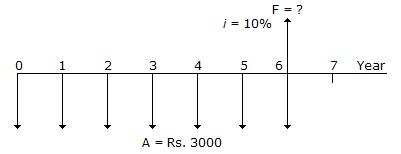
\includegraphics{../data_img/engineering-economics-_1525417448-22.png}
}
\begin{enumerate}[label=\Alph*.]
\item{Equal deposits of Rs. 3000 per year }
\item{The rate of interest is 10\% per year account}
\item{The amount accumulated after the seventh deposit is to be computed}
\item{All of these}
\end{enumerate}
\item{In the cash flow diagram shown in the given figure \\

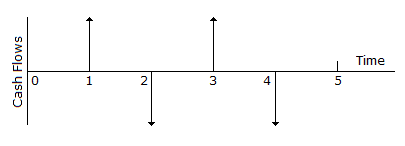
\includegraphics{../data_img/engineering-economics-_1525417499-24.png}
}
\begin{enumerate}[label=\Alph*.]
\item{The first disbursement occurs at the end of year 2}
\item{The second disbursement occurs at the end of year 4}
\item{The first receipt occurs at the end of year 1}
\item{All of these}
\end{enumerate}
\item{Refer to the cash flow diagram of uniform gradient in a cash flow (in the given figure), the gradient is: \\

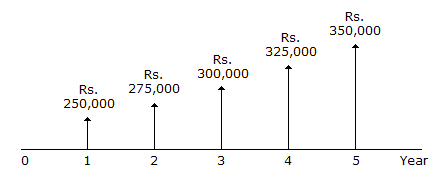
\includegraphics{../data_img/engineering-economics-_1525417531-23.png}
}
\begin{enumerate}[label=\Alph*.]
\item{Rs. 10000 per year}
\item{Rs. 15000 per year}
\item{Rs. 20000 per year}
\item{Rs. 25000 per year}
\end{enumerate}
\item{A loan of P5,000 is made for a period of 15 months, at a simple interest rate of 15\%, what future amount is due at the end of the loan period?}
\\\begin{enumerate*}[itemjoin=\qquad, label=\Alph*.]
\item{5,937.50}
\item{5,873.20}
\item{5,712.40}
\item{5,690.12}
\end{enumerate*}
\item{A P 1,000,000 issue of 3\%, 15-year bond was sold at 95\%. What is the rate of interest of this investment?}
\\\begin{enumerate*}[itemjoin=\qquad, label=\Alph*.]
\item{3.0\%}
\item{3.4\%}
\item{3.7\%}
\item{4.0\%}
\end{enumerate*}
\item{A investor wishes to earn 7\% on his capital after payment of taxes. If the income from an available investment will be taxed at an average rate of 42\%, what minimum rate of return, before payment of taxes, must the investment offer to be justified?}
\\\begin{enumerate*}[itemjoin=\qquad, label=\Alph*.]
\item{12.07 \%}
\item{12.34 \%}
\item{12.67 \%}
\item{12.87 \%}
\end{enumerate*}
\item{What refers to the value of an asset which a disinterested third party, different from the buyer and seller, will determine in order to establish a price acceptable to both parties?}
\begin{enumerate}[label=\Alph*.]
\item{Book value}
\item{Market value}
\item{Fair value}
\item{Franchise value}
\end{enumerate}
\item{What is another term for ``current assets''?
}
\begin{enumerate}[label=\Alph*.]
\item{Fixed assets}
\item{Non-liquid assets}
\item{Liquid assets}
\item{Ccash}
\end{enumerate}
\item{What is the ordinary interest on P1,500.50 for 182 days at 5.2\%?}
\\\begin{enumerate*}[itemjoin=\qquad, label=\Alph*.]
\item{P39.01}
\item{P39.82}
\item{P39.45}
\item{P39.99}
\end{enumerate*}
\item{In what method of computing depreciation where it assumes that a sinking fund is established in which funds will accumulate for replacement purposes?}
\begin{enumerate}[label=\Alph*.]
\item{Straight line method}
\item{Sinking fund method}
\item{Sum-of-year digit method}
\item{Declining balance method}
\end{enumerate}
\item{What is another term for ``acid-test ratio''?
}
\begin{enumerate}[label=\Alph*.]
\item{Current ratio}
\item{Quick ratio}
\item{Profit margin ratio}
\item{Price-earnings ratio}
\end{enumerate}
\item{What refers to the amount of a product made available for sale?}
\\\begin{enumerate*}[itemjoin=\qquad, label=\Alph*.]
\item{Supply}
\item{Demand}
\item{Product}
\item{Good}
\end{enumerate*}
\item{What refers to the cost of borrowing money or the amount earned by a unit principal per unit time?}
\begin{enumerate}[label=\Alph*.]
\item{Yield rate}
\item{Rate of return}
\item{Rate of interest}
\item{Economic return}
\end{enumerate}
\item{What is the market situation exist when there are many buyers and many sellers?}
\begin{enumerate}[label=\Alph*.]
\item{Perfect competition}
\item{Oligopoly}
\item{Oligopsony}
\item{Monopoly}
\end{enumerate}
\item{The product of CAF (SP) and PWF (SP) is:}
\\\begin{enumerate*}[itemjoin=\qquad, label=\Alph*.]
\item{$ \frac{1}{2} $}
\item{$ 1 $}
\item{$ \frac{1}{3} $}
\item{$ \frac{1}{4} $}
\end{enumerate*}
\item{In a cash-flow diagram:}
\begin{enumerate}[label=\Alph*.]
\item{Time 0 is considered to be the present}
\item{Time 1 is considered to be the end of time period 1}
\item{A vertical arrow pointing up indicates a positive cash flow}
\item{All of these}
\end{enumerate}
\item{Lands, buildings, plants and machineries are example of what type of asset?}
\begin{enumerate}[label=\Alph*.]
\item{Current asset}
\item{Trade investment asset}
\item{Fixed asset}
\item{Intangible asset}
\end{enumerate}
\item{What represents the ownership of stockholders who have a residual claim on the assets of the corporation after all other claims have been settled?}
\begin{enumerate}[label=\Alph*.]
\item{Authorized capital stock}
\item{Preferred stock}
\item{Incorporator stock}
\item{Common stock}
\end{enumerate}
\item{The institute of Electronics and Communications Engineers of the Philippines (IECEP) is planning to put up its own building. Two proposals being considered are: \\
A. The construction of the building now to cost P 400,000 \\
B. The construction of a smaller building now to cost P300,000 and at the end of 5 years, an extension to be added to cost P 200,000. \\
By how much is proposal B more economical than proposal A if interest rate is 20\% and depreciation to be neglected? \\
}
\\\begin{enumerate*}[itemjoin=\qquad, label=\Alph*.]
\item{P 19,122.15}
\item{P 19,423.69}
\item{P 19,518.03}
\item{P 19,624.49}
\end{enumerate*}
\item{What refers to the residual value of a company's assets after all outside liabilities (shareholders excluded) have been allowed for?
}
\\\begin{enumerate*}[itemjoin=\qquad, label=\Alph*.]
\item{Dividend}
\item{Equity}
\item{Return}
\item{Par value}
\end{enumerate*}
\item{What refers to the amount of money paid for the use of borrowed capital?}
\begin{enumerate}[label=\Alph*.]
\item{Interest}
\item{Rate of interest}
\item{Simple interest}
\item{Principal}
\end{enumerate}
\item{Which is true about corporation?}
\begin{enumerate}[label=\Alph*.]
\item{It is worse type of business organization.}
\item{The minimum number of incorporators to start a corporation is three.}
\item{Its life is dependent on the lives of the incorporators.}
\item{The stock holders of the corporation are only liable to the extent of their investments.}
\end{enumerate}
\item{Which is true about partnership?}
\begin{enumerate}[label=\Alph*.]
\item{It has a perpetual life.}
\item{It will be dissolved if one of the partners ceases to be connected with the partnership.}
\item{It can be handed down from one generation of partners to another.}
\item{Its capitalization must be equal for each partner.}
\end{enumerate}
\item{What refers to the interest rate at which the present work of the cash flow on a project is zero of the interest earned by an investment?}
\begin{enumerate}[label=\Alph*.]
\item{Economic return}
\item{Yield}
\item{Rate of return}
\item{Return of investment}
\end{enumerate}
\item{Capitalized cost of any structure or property is computed by which formula?}
\begin{enumerate}[label=\Alph*.]
\item{First cost + interest of first cost}
\item{Annual cost - interest of first cost}
\item{First cost + cost of perpetual maintenance}
\item{First cost + salvage value}
\end{enumerate}
\item{The more critical (or severe) test of the firm's liquidity can be judged by:}
\begin{enumerate}[label=\Alph*.]
\item{Liquidity ratio}
\item{Current ratio}
\item{Acid-Test (or Quick) ratio}
\item{Debts ratio}
\end{enumerate}
\item{In a cash flow series:}
\begin{enumerate}[label=\Alph*.]
\item{Uniform gradient signifies that an income or disbursement changes by the same amount in each interest period}
\item{Either an increase or decrease in the amount of a cash flow is called the gradient}
\item{The gradient in the cash flow may be positive or negative}
\item{All of these}
\end{enumerate}
\item{A VOM has a selling price of P 400. If its selling price is expected to decline at a rate of 10\% per annum due to obsolescence, what will be its selling price after 5 years?}
\\\begin{enumerate*}[itemjoin=\qquad, label=\Alph*.]
\item{P 222.67}
\item{P 212.90}
\item{P 236.20}
\item{P 231.56}
\end{enumerate*}
\item{The monthly demand for ice cans being manufactured by Mr. Camus is 3200 pieces. With a manual operated guillotine, the unit cutting cost is P25.00. An electrically operated hydraulic guillotine was offered to Mr. Camus at a price of P275,000.00 and which cuts by 30\% the unit cutting cost. Disregarding the cost of money, how many months will Mr. Camus be able to recover the cost of the machine if he decides to buy now?}
\\\begin{enumerate*}[itemjoin=\qquad, label=\Alph*.]
\item{10 months}
\item{11 months}
\item{12 months}
\item{13 months}
\end{enumerate*}
\item{The key to profitable operation for project cost control, is:}
\begin{enumerate}[label=\Alph*.]
\item{To keep the project cost equal to original cost estimate}
\item{To keep the project cost equal to subsequent construction budget}
\item{To keep the project cost within the cost budget and knowing when and where job costs are deviating}
\item{None of these}
\end{enumerate}
\item{What is an accounting term that represents an inventory account adjustment?}
\begin{enumerate}[label=\Alph*.]
\item{Cost of goods sold}
\item{Cost accounting}
\item{Standard cost}
\item{Overhead cost}
\end{enumerate}
\item{Current ratio is:}
\\\begin{enumerate*}[itemjoin=\qquad, label=\Alph*.]
\item{$ \frac{{{\text{Current assets}}}}{{{\text{Current liabilities}}}} $}
\item{$ \frac{{{\text{Current assets}} + {\text{Loans}}}}{{{\text{Current liabilities}}}} $}
\item{$ \frac{{{\text{Current assets}} + {\text{Loans advances}}}}{{{\text{Current liabilities}}}} $}
\item{None of these}
\end{enumerate*}
\end{enumerate}
\textbf{Answer Key}
\begin{tabular}{ | c | c c c c c c c c c c | }
\hline
 & 1 & 2 & 3 & 4 & 5 & 6 & 7 & 8 & 9 & 0 \\
\hline
0 & C & A & D & C & B & B & C & A & A & C \\
10 & D & B & D & A & D & B & C & B & C & B \\
20 & D & A & B & B & B & A & A & C & C & D \\
30 & D & D & C & C & D & B & D & C & D & D \\
40 & D & A & A & A & C & C & C & B & B & A \\
50 & C & A & B & D & C & D & D & B & A & D \\
60 & C & C & C & C & D & C & C & C & B & A \\
\hline
\end{tabular}
\clearpage
\subsection*{Section 2}
\begin{enumerate}
\item{Under ordinary simple interest, how many days in one year?}
\\\begin{enumerate*}[itemjoin=\qquad, label=\Alph*.]
\item{300}
\item{360}
\item{365}
\item{366}
\end{enumerate*}
\item{The original record of a business transaction is recorded in this book.}
\\\begin{enumerate*}[itemjoin=\qquad, label=\Alph*.]
\item{Work book}
\item{Journal}
\item{Ledger}
\item{Account book}
\end{enumerate*}
\item{What are the common methods of computing depletion charge?}
\begin{enumerate}[label=\Alph*.]
\item{Rational method and irrational method}
\item{Conservative method and conventional method}
\item{Unit method and percentage method}
\item{Discrete method and depletion allowance method}
\end{enumerate}
\item{A factory operator bought a diesel generator set for P 10,000.00 and agreed to pay the dealer uniform sum at the end of each year for 5 years at 8\% interest compounded annually, that the final payment will cancel the debt for principal and interest. What is the annual payment?}
\\\begin{enumerate*}[itemjoin=\qquad, label=\Alph*.]
\item{P 2,500.57}
\item{P 2,544.45}
\item{P 2,540.56}
\item{P 2,504.57}
\end{enumerate*}
\item{What refers to the goods and services that are desired by human and will be acquired only after all the needs have been satisfied?}
\begin{enumerate}[label=\Alph*.]
\item{Producer products}
\item{Consumer products}
\item{Luxury}
\item{Necessity}
\end{enumerate}
\item{Shell Philippines, a multinational company, has a total gross income for a particular year of P 50,000,000. The taxable income after taking all deductions except for depletion is P 18,500,000. What is the allowable depletion allowance for that particular year? Take percentage of gross income for oil as 22\%.}
\\\begin{enumerate*}[itemjoin=\qquad, label=\Alph*.]
\item{P 9,358.41}
\item{P 9,228.45}
\item{P 9,250.00}
\item{P 9,308.45}
\end{enumerate*}
\item{What annuity is required over 12 years to equate with a future amount of P 20,000? Assume i= 6\% annually.}
\\\begin{enumerate*}[itemjoin=\qquad, label=\Alph*.]
\item{P 1,290.34}
\item{P 1,185.54}
\item{P 1,107.34}
\item{P 1,205.74}
\end{enumerate*}
\item{Both architect and engineer make use of the cost estimate of the project:}
\begin{enumerate}[label=\Alph*.]
\item{For site selection}
\item{For designing of the project}
\item{For choosing alternatives}
\item{All of these}
\end{enumerate}
\item{What refers to the present worth of cost associated with an asset for an infinite period of time?}
\begin{enumerate}[label=\Alph*.]
\item{Annual cost}
\item{Increment cost}
\item{Capitalized cost}
\item{Operating cost}
\end{enumerate}
\item{The interest calculated on the basis of 365 days a year, is known as:}
\begin{enumerate}[label=\Alph*.]
\item{Interest}
\item{Ordinary simple interest}
\item{Exact simple interest}
\item{None of these}
\end{enumerate}
\item{An asset is purchased for P 9,000.00. Its estimated economic life is 10 years after which it will be sold for P 1,000.00. Find the depreciation in the first three years using sum-of-years digit method}
\\\begin{enumerate*}[itemjoin=\qquad, label=\Alph*.]
\item{P 3,279.27}
\item{P 3,927.27}
\item{P 3,729.27}
\item{P 3,792.72}
\end{enumerate*}
\item{What is another term for ``perfect competition''?
}
\begin{enumerate}[label=\Alph*.]
\item{Atomistic competition}
\item{No-limit competition}
\item{Free-for-all competition}
\item{Heterogeneous market}
\end{enumerate}
\item{A person buys a piece of lot for P 100,000 downpayment and 10 deferred semi-annual payments of P 8,000 each, starting three years from now. What is the present value of the investment if the rate of interest is 12\% compounded semi-annually?}
\\\begin{enumerate*}[itemjoin=\qquad, label=\Alph*.]
\item{P 142,999.08}
\item{P 143,104.89}
\item{P 142,189.67}
\item{P 143,999.08}
\end{enumerate*}
\item{Mr. Jun Ramos was granted a loan of P20,000 by his employer Excel First Review and Training Center, Inc. with an interest of 6\% for 180 days on the principal collected in advance. The corporation would accept a promissory note for P20,000 non-interest for 180 days. If discounted at once, find the proceeds of the note.}
\\\begin{enumerate*}[itemjoin=\qquad, label=\Alph*.]
\item{P18,000}
\item{P18,900}
\item{P19,000}
\item{P19,100}
\end{enumerate*}
\item{What is the feature of some bonds whereby the issuer can redeem it before it matures?}
\\\begin{enumerate*}[itemjoin=\qquad, label=\Alph*.]
\item{Return clause}
\item{Callability}
\item{Recall clause}
\item{Call class}
\end{enumerate*}
\item{Present worth Annuity (PWA) is generally known as}
\begin{enumerate}[label=\Alph*.]
\item{Premium annuities}
\item{Income annuities}
\item{Future annuities}
\item{All of these}
\end{enumerate}
\item{A leading shoe manufacturer produces a pair of Lebron James signature shoes at a labor cost of P 900.00 a pair and a material cost of P 800.00 a pair. The fixed charges on the business are P 5,000,000 a month and the variable costs are P 400.00 a pair. Royalty to Lebron James is P 1,000 per pair of shoes sold. If the shoes sell at P 5,000 a pair, how many pairs must be produced each month for the manufacturer to break-even?}
\\\begin{enumerate*}[itemjoin=\qquad, label=\Alph*.]
\item{2.590}
\item{2,632}
\item{2,712}
\item{2,890}
\end{enumerate*}
\item{Duopsony is a market situation where there is/are:}
\begin{enumerate}[label=\Alph*.]
\item{Few sellers and few buyers}
\item{Few sellers and many buyers}
\item{Many sellers and few buyers}
\item{One seller and few buyers}
\end{enumerate}
\item{Duopoly is a market situation where there is/are:}
\begin{enumerate}[label=\Alph*.]
\item{Few sellers and few buyers}
\item{Few sellers and many buyers}
\item{Many sellers and few buyers}
\item{One seller and few buyers}
\end{enumerate}
\item{What is the present worth of two P 100 payments at the end of the third year and fourth year? The annual interest rate is 8\%.}
\\\begin{enumerate*}[itemjoin=\qquad, label=\Alph*.]
\item{P 150.56}
\item{P 152.88}
\item{P 153.89}
\item{P 151.09}
\end{enumerate*}
\item{What refers to the market situation in which any given product is supplied by a very large number of vendors and there is no restriction against additional vendors from entering the market?}
\begin{enumerate}[label=\Alph*.]
\item{Perfect competition}
\item{Oligopoly}
\item{Oligopsony}
\item{Monopoly}
\end{enumerate}
\item{The functional depreciation is sometimes called \_\_\_\_\_\_.}
\begin{enumerate}[label=\Alph*.]
\item{Demand depreciation}
\item{Adolescence}
\item{Life depreciation}
\item{Failure depreciation}
\end{enumerate}
\item{What is the simplest form of business organization?}
\begin{enumerate}[label=\Alph*.]
\item{Sole proprietorship}
\item{Partnership}
\item{Enterprise}
\item{Corporation}
\end{enumerate}
\item{Double taxation is a disadvantage of which business organization?}
\begin{enumerate}[label=\Alph*.]
\item{Sole proprietorship}
\item{Partnership}
\item{Corporation}
\item{Enterprise}
\end{enumerate}
\item{What is the present worth of a P500 annuity starting at the end of the third year and continuing to the end of the fourth year, if the annual interest rate is 10 \%?}
\\\begin{enumerate*}[itemjoin=\qquad, label=\Alph*.]
\item{P 727.17}
\item{P 717.17}
\item{P 714.71}
\item{P 731.17}
\end{enumerate*}
\item{You borrow P3,500.00 for one year from a friend at an interest rate of 1.5\% per month instead of taking a loan from a bank at a rate of 18\% per year. How much lesser you will pay by borrowing the money from the bank?}
\\\begin{enumerate*}[itemjoin=\qquad, label=\Alph*.]
\item{P 62.44}
\item{P44.55}
\item{P54.66}
\item{P37.56}
\end{enumerate*}
\item{What refers to the negotiable claim issued by a bank in lien of a term deposit?}
\begin{enumerate}[label=\Alph*.]
\item{Time deposit}
\item{Bond}
\item{Capital gain certificate}
\item{Certificate of deposit}
\end{enumerate}
\item{If `a' is the base amount expenditure, `b' is the increase in the operation cost each year over a period of' 'n' years, the total cost of maintenance is:
}
\\\begin{enumerate*}[itemjoin=\qquad, label=\Alph*.]
\item{a + (n + 1) b}
\item{a + (n - 1) b}
\item{a $\times$ (n - 1) b}
\item{a - (n - 1) b}
\end{enumerate*}
\item{A \_\_\_\_\_\_ is a market situation where economies of scale are so significant that cost are only minimized when the entire output of an industry is supplied by a single producer so that the supply costs are lower under monopoly that under perfect competition.}
\begin{enumerate}[label=\Alph*.]
\item{Perfect monopoly}
\item{Bilateral monopoly}
\item{Natural monopoly}
\item{Ordinary monopoly}
\end{enumerate}
\item{Aside from many sellers and many buyers, which one is a characteristic of perfect competition?}
\begin{enumerate}[label=\Alph*.]
\item{Homogeneous product}
\item{Free market entry and exit}
\item{Perfect information and absence of all economic friction}
\item{All of the above}
\end{enumerate}
\item{What is the opposite of perfect competition?}
\\\begin{enumerate*}[itemjoin=\qquad, label=\Alph*.]
\item{Monopsony}
\item{Oligopoly}
\item{Oligopsony}
\item{Monopoly}
\end{enumerate*}
\item{What is the factor name of the formula (1 + i)\^{}-n?}
\begin{enumerate}[label=\Alph*.]
\item{Uniform gradient future worth}
\item{Capital recovery}
\item{Single payment present worth}
\item{Single payment compound amount}
\end{enumerate}
\item{What is defined as a financial security note issued by business or corporation and by the government as a means of borrowing long-term fund?}
\\\begin{enumerate*}[itemjoin=\qquad, label=\Alph*.]
\item{T-bills}
\item{Securities}
\item{Bond}
\item{Bank notes}
\end{enumerate*}
\item{What is defines as the analysis and evaluation of the monetary consequences by using the theories and principles of economics to engineering applications, designs and projects?}
\begin{enumerate}[label=\Alph*.]
\item{Economic Analysis}
\item{Engineering cost analysis}
\item{Engineering economy}
\item{Design cost analysis}
\end{enumerate}
\item{What is a market situation whereby there is only one buyer of an item for which there is no goods substitute?}
\\\begin{enumerate*}[itemjoin=\qquad, label=\Alph*.]
\item{Monopsony}
\item{Monopoly}
\item{Oligopoly}
\item{Oligopsony}
\end{enumerate*}
\item{The person desires to pay off the amount in 10 equal annual instalments. The amount of each installment is:}
\\\begin{enumerate*}[itemjoin=\qquad, label=\Alph*.]
\item{Rs. 5638}
\item{Rs. 6638}
\item{Rs. 7738}
\item{None of these}
\end{enumerate*}
\item{Oligopoly exists when there is/are:}
\begin{enumerate}[label=\Alph*.]
\item{Few sellers and few buyers}
\item{Few sellers and many buyers}
\item{Many sellers and few buyers}
\item{One seller and few buyers}
\end{enumerate}
\item{Under the depletion allowance method in computing depreciation, the depletion charge is equal to either \_\_\_\_\_\_ whichever is smaller.}
\begin{enumerate}[label=\Alph*.]
\item{Fixed percentage of gross income or the net taxable income}
\item{Fixed percentage of gross income or 50\% of the net taxable income}
\item{50\% of the fixed percentage of gross income or 50\% of the net taxable income}
\item{50\% of the fixed percentage of gross income or the net taxable income}
\end{enumerate}
\item{What is used to record historical financial transactions?}
\begin{enumerate}[label=\Alph*.]
\item{Bookkeeping system}
\item{Ledger system}
\item{Balance check}
\item{General journal system}
\end{enumerate}
\item{A machine costs of P 8,000 and an estimated life of 10 years with a salvage value of P 500. What is its book value after 8 years using straight line method?}
\\\begin{enumerate*}[itemjoin=\qquad, label=\Alph*.]
\item{P 2,000.00}
\item{P 2,100.00}
\item{P 2,200.00}
\item{P 2,300.00}
\end{enumerate*}
\item{The ratio obtained by dividing 'quick assets' by current liabilities is called}
\begin{enumerate}[label=\Alph*.]
\item{Turnover ratio}
\item{Acid test ratio}
\item{Solvency ratio}
\item{None of these}
\end{enumerate}
\item{What is the type of annuity where the first payment does not begin until some later date in the cash flow?}
\begin{enumerate}[label=\Alph*.]
\item{Ordinary annuity}
\item{Perpetuity}
\item{Annuity due}
\item{Deferred annuity}
\end{enumerate}
\item{The alternatives which are standalone solutions for given situations in engineering involve:}
\begin{enumerate}[label=\Alph*.]
\item{A purchase cost (first cost)}
\item{The anticipated life of the assets}
\item{The anticipated resalable value (salvage value) and the interest return (rate of return)}
\item{All of these}
\end{enumerate}
\item{Which of the following is an example of intangible asset?}
\begin{enumerate}[label=\Alph*.]
\item{Cash}
\item{Investment in subsidiary companies}
\item{Furnitures}
\item{Patents}
\end{enumerate}
\item{What do you call the after-tax present worth of all depreciation effects over the depreciation period of the asset?}
\begin{enumerate}[label=\Alph*.]
\item{Asset recovery}
\item{Depreciation recovery}
\item{Period recovery}
\item{After-tax recovery}
\end{enumerate}
\item{If there is only one seller and many buyers, the market situation is \_\_\_\_\_\_\_\_ .}
\\\begin{enumerate*}[itemjoin=\qquad, label=\Alph*.]
\item{Duopsony}
\item{Oligopoly}
\item{Oligopsony}
\item{Monopoly}
\end{enumerate*}
\item{What type of bond where the corporation's owner name are recorded and the interest is paid periodically to the owners with their asking for it?
}
\begin{enumerate}[label=\Alph*.]
\item{Preferred bond}
\item{Registered bond}
\item{Incorporators bond}
\item{Callable bond}
\end{enumerate}
\item{As applied to capitalized asset, the distribution of the initial cost by a periodic changes to operation as in depreciation or the reduction of a debt by either periodic or irregular prearranged programs is called \_\_\_\_\_\_.}
\begin{enumerate}[label=\Alph*.]
\item{Annuity}
\item{Amortization}
\item{Capital recovery}
\item{Annuity factor}
\end{enumerate}
\item{A uniform series of payment occurring at equal interval of time is called \_\_\_\_\_\_.}
\\\begin{enumerate*}[itemjoin=\qquad, label=\Alph*.]
\item{Annuity}
\item{Amortization}
\item{Depreciation}
\item{Bond}
\end{enumerate*}
\item{The flow back of profit plus depreciation form a given project is called \_\_\_\_\_\_.}
\begin{enumerate}[label=\Alph*.]
\item{Capital recovery}
\item{Cash flow}
\item{Economic return}
\item{Earning value}
\end{enumerate}
\item{A form of business firm which is owned and run by a group of individuals for their mutual benefit is called \_\_\_\_\_\_.}
\\\begin{enumerate*}[itemjoin=\qquad, label=\Alph*.]
\item{Cooperative}
\item{Corporation}
\item{Enterprise}
\item{Partnership}
\end{enumerate*}
\item{The ratio of the net income before taxes to net sales is called \_\_\_\_\_\_.}
\begin{enumerate}[label=\Alph*.]
\item{Current ratio}
\item{Inventory turnover}
\item{Profit margin ratio}
\item{Price-earnings ratio}
\end{enumerate}
\item{The difference between the present and future worth of money at some time in the future is called \_\_\_\_\_\_.}
\\\begin{enumerate*}[itemjoin=\qquad, label=\Alph*.]
\item{Discount}
\item{Deduction}
\item{Inflation}
\item{Depletion}
\end{enumerate*}
\item{The amount of company's profit that the board of directors of the corporation decides to distribute to ordinary shareholders is called \_\_\_\_\_\_.
}
\\\begin{enumerate*}[itemjoin=\qquad, label=\Alph*.]
\item{Dividend}
\item{Return}
\item{Share of stock}
\item{Equity}
\end{enumerate*}
\item{An association of two or more persons for the purpose of engaging into a business for profit is called \_\_\_\_\_\_.}
\begin{enumerate}[label=\Alph*.]
\item{Entrepreneurship}
\item{Partnership}
\item{Proprietorship}
\item{Corporation}
\end{enumerate}
\item{The amount of property in which a willing buyer to a willing seller for the property when neither one is under the compulsion to buy nor to sell is called \_\_\_\_\_\_.}
\begin{enumerate}[label=\Alph*.]
\item{Fair value}
\item{Market value}
\item{Good will value}
\item{Book value}
\end{enumerate}
\item{The process of determining the value or worth of a physical property for specific reason is called \_\_\_\_\_\_.}
\\\begin{enumerate*}[itemjoin=\qquad, label=\Alph*.]
\item{Investment}
\item{Valuation}
\item{Economy}
\item{Depletion}
\end{enumerate*}
\item{A bond without any security behind them except a promise to pay by the issuing corporation is called \_\_\_\_\_\_.}
\\\begin{enumerate*}[itemjoin=\qquad, label=\Alph*.]
\item{Joint bond}
\item{Debenture bond}
\item{Trust bond}
\item{Common bond}
\end{enumerate*}
\item{A mathematical expression also known as the present value of annuity of one is called \_\_\_\_\_\_.}
\begin{enumerate}[label=\Alph*.]
\item{Load factor}
\item{Demand factor}
\item{Sinking fund factor}
\item{Present worth factor}
\end{enumerate}
\item{The first cost to be incurred if the piece of equipment now in place had been bought for a second hand dealer or some other business is called \_\_\_\_\_\_.}
\\\begin{enumerate*}[itemjoin=\qquad, label=\Alph*.]
\item{Material cost}
\item{Fixed cost}
\item{First cost}
\item{In-place value}
\end{enumerate*}
\item{All the proceeds which are received by the business as a result of the sale of goods is called \_\_\_\_\_\_.}
\\\begin{enumerate*}[itemjoin=\qquad, label=\Alph*.]
\item{Net income}
\item{Gross income}
\item{Net revenue}
\item{Total sales}
\end{enumerate*}
\item{The price at which the callable bond will be redeemed from the bondholder is called \_\_\_\_\_\_.}
\begin{enumerate}[label=\Alph*.]
\item{Par value}
\item{Call value}
\item{Face value}
\item{Redemption value}
\end{enumerate}
\item{Aggregation of individuals formed for the purpose of conducting a business and recognized by law as a fictitious person is called \_\_\_\_\_\_.}
\\\begin{enumerate*}[itemjoin=\qquad, label=\Alph*.]
\item{Partnership}
\item{Investors}
\item{Corporation}
\item{Stockholders}
\end{enumerate*}
\item{A type of bond to which are attached coupons indicating the interest due and the date when such interest is to be paid is called \_\_\_\_\_\_.}
\begin{enumerate}[label=\Alph*.]
\item{Registered bond}
\item{Coupon bond}
\item{Mortgage bond}
\item{Collateral trust bond}
\end{enumerate}
\item{The unrecovered depreciation which results due to poor estimates as to the life of the equipment is called \_\_\_\_\_\_.}
\\\begin{enumerate*}[itemjoin=\qquad, label=\Alph*.]
\item{Sunk cost}
\item{Economic life}
\item{In-place value}
\item{Annuity}
\end{enumerate*}
\item{What do you call a one-time credit against taxes?}
\begin{enumerate}[label=\Alph*.]
\item{Due credit}
\item{Tax credit}
\item{Credible credit}
\item{Revenue credit}
\end{enumerate}
\item{A feasibility study shows that a fixed capital investment of P10,000,000 is required for a proposed construction firm and an estimated working capital of P2,000,000. Annual depreciation is estimated to be10\% of the fixed capital investment. Determine the rate of return on the total investment if the annual profit is P3,500,000.}
\\\begin{enumerate*}[itemjoin=\qquad, label=\Alph*.]
\item{28.33 \%}
\item{29.17 \%}
\item{30.12 \%}
\item{30.78 \%}
\end{enumerate*}
\item{What is the type of annuity that does not have a fixed time span but continues indefinitely or forever?}
\begin{enumerate}[label=\Alph*.]
\item{Ordinary annuity}
\item{Perpetuity}
\item{Annuity due}
\item{Deferred annuity}
\end{enumerate}
\item{The ratio of current assets to current liabilities is known as}
\begin{enumerate}[label=\Alph*.]
\item{Liquidity ratio}
\item{Current ratio}
\item{Acid-Test (or Quick) ratio}
\item{Debts ratio}
\end{enumerate}
\item{Current assets less inventories divided by current liabilities is known as}
\begin{enumerate}[label=\Alph*.]
\item{Liquidity ratio}
\item{Current ratio}
\item{Acid-Test (or Quick) ratio}
\item{Debts ratio}
\end{enumerate}
\end{enumerate}
\textbf{Answer Key}
\begin{tabular}{ | c | c c c c c c c c c c | }
\hline
 & 1 & 2 & 3 & 4 & 5 & 6 & 7 & 8 & 9 & 0 \\
\hline
0 & B & B & C & D & D & C & B & D & C & C \\
10 & B & A & D & A & B & D & B & C & B & B \\
20 & A & B & A & C & B & C & D & B & C & D \\
30 & D & C & C & A & B & A & B & B & A & A \\
40 & B & D & D & D & B & D & B & B & A & B \\
50 & A & C & A & A & B & B & B & B & D & D \\
60 & B & B & C & B & A & B & B & B & B & C \\
\hline
\end{tabular}
\clearpage
\subsection*{Section 3}
\begin{enumerate}
\item{A type of bond where the corporation pledges securities which it owns such as the stock or bonds of one of its subsidiaries.}
\begin{enumerate}[label=\Alph*.]
\item{Mortgage bond}
\item{Joint bond}
\item{Security bond}
\item{Collateral trust bond}
\end{enumerate}
\item{What is a measure of the average speed with which accounts receivable are collected?}
\begin{enumerate}[label=\Alph*.]
\item{Current ratio}
\item{Quick ratio}
\item{Acid test ratio}
\item{Receivable turnover}
\end{enumerate}
\item{What is the change in cost per unit variable change called?}
\begin{enumerate}[label=\Alph*.]
\item{Variable cost}
\item{Incremental cost}
\item{Fixed cost}
\item{Supplemental cost}
\end{enumerate}
\item{What refers to the saving which takes place because goods are not available for consumption rather than consumer really want to save?}
\begin{enumerate}[label=\Alph*.]
\item{Compulsory saving}
\item{Consumer saving}
\item{Forced saving}
\item{All of the above}
\end{enumerate}
\item{Cash money and credit necessary to establish and operate an enterprise are generally called \_\_\_\_\_\_.}
\\\begin{enumerate*}[itemjoin=\qquad, label=\Alph*.]
\item{Capital}
\item{Funds}
\item{Assets}
\item{Liabilities}
\end{enumerate*}
\item{What is an index of short-term paying ability?}
\begin{enumerate}[label=\Alph*.]
\item{Price-earnings ratio}
\item{Current ratio}
\item{Profit margin ratio}
\item{Gross margin}
\end{enumerate}
\item{Which one of the following statements is correct?}
\begin{enumerate}[label=\Alph*.]
\item{The number of years required to recover the initial cash investment in a project, is called Pay Back period (PBP)}
\item{The discount rate that equates the present value of the expected Net Cash Flows (CFs) with the Initial Cash Outflow (ICO) is known as internal rate of return}
\item{The present value of the proposal's net cash flows, less the proposal's initial cash outflow is known as the Net Present Value (NPV)}
\item{All of these}
\end{enumerate}
\item{If a seller recovers his capital along with accumulated compensating interest not in one single lump-sum payment but in periodical equal payments, over time:}
\begin{enumerate}[label=\Alph*.]
\item{Capital Recovery Annuity fs availed}
\item{Present work Annuity is availed}
\item{Sinking Fund Annuity is availed}
\item{Sinking Fund Annuity is availed}
\end{enumerate}
\item{What is defined as the investment of loan or principal which is based not only on the original amount of the loan or principal but the amount of loaned or principal plus the previous accumulated interest?}
\begin{enumerate}[label=\Alph*.]
\item{Effective rate of interest}
\item{Nominal rate of interest}
\item{Compound interest}
\item{Simple interest}
\end{enumerate}
\item{What refers to the value of an intangible item which arises from the exclusive right of a company to provide a specified product and service in a certain region of the country?}
\begin{enumerate}[label=\Alph*.]
\item{Company value}
\item{Going value}
\item{Goodwill value}
\item{Franchise value}
\end{enumerate}
\item{What stock represents ownership and enjoys certain preferences than ordinary stock?}
\begin{enumerate}[label=\Alph*.]
\item{Authorized stock}
\item{Preferred stock}
\item{Incorporator's stock}
\item{Presidential stock}
\end{enumerate}
\item{What is the factor name of the formula $$\left[ {\frac{{{\text{i}}{{\left( {1 + {\text{i}}} \right)}^{\text{n}}}}}{{{{\left( {1 + {\text{i}}} \right)}^{\text{n}}} - 1}}} \right]?$$}
\begin{enumerate}[label=\Alph*.]
\item{Uniform series sinking fund}
\item{Capital recovery}
\item{Single payment present worth}
\item{Uniform gradient future worth}
\end{enumerate}
\item{The financial analysis:}
\begin{enumerate}[label=\Alph*.]
\item{Helps a share holder to compare the expected return on his investment in the firm against the expected return from other alternative investment}
\item{Helps a bank to know the financial position of the firm for granting a loan to the firm}
\item{Helps to judge the success of the firm's financial plans}
\item{All of these}
\end{enumerate}
\item{What refers to a document that shows proof of legal ownership of a financial security?}
\\\begin{enumerate*}[itemjoin=\qquad, label=\Alph*.]
\item{Bond}
\item{Bank note}
\item{Coupon}
\item{Check}
\end{enumerate*}
\item{What refers to the exchange mechanism that brings together the sellers and the buyers of a product, factor of production or financial security?}
\\\begin{enumerate*}[itemjoin=\qquad, label=\Alph*.]
\item{Mall}
\item{Market}
\item{Store}
\item{Office}
\end{enumerate*}
\item{What denotes in the fall in the exchange rate of one currency in terms of the others? This term is usually applies to the floating exchange rate.}
\begin{enumerate}[label=\Alph*.]
\item{Currency appreciation}
\item{Currency depreciation}
\item{Currency devaluation}
\item{Currency float}
\end{enumerate}
\item{In what method of computing depreciation where it assumes that the annual cost of depreciation is a fixed percentage of the book value at the beginning of the year?}
\begin{enumerate}[label=\Alph*.]
\item{Straight line method}
\item{Sinking fund method}
\item{Sum-of-year digit method}
\item{Declining balance method}
\end{enumerate}
\item{The sunk costs include:}
\begin{enumerate}[label=\Alph*.]
\item{A past expenditure}
\item{An unrecovered balance}
\item{An invested capital that cannot be retrieved}
\item{All of these}
\end{enumerate}
\item{Miss Evilla borrowed money from a bank. She receives from the bank P1,340.00 and promised to pay P1,500.00 at the end of 9 months. Determine the corresponding discount rate or often referred to as the ``banker's discount''.
}
\\\begin{enumerate*}[itemjoin=\qquad, label=\Alph*.]
\item{13.15 \%}
\item{13.32 \%}
\item{13.46 \%}
\item{13.73 \%}
\end{enumerate*}
\item{Annuities involve:}
\begin{enumerate}[label=\Alph*.]
\item{A series of payments}
\item{All payments of equal amount}
\item{Payment at equal time intervals}
\item{All of these}
\end{enumerate}
\item{An amount of P1,000 becomes P1,608.44 after 4 years compounded bimonthly. Find the nominal interest.}
\\\begin{enumerate*}[itemjoin=\qquad, label=\Alph*.]
\item{11.89 \%}
\item{12.00 \%}
\item{12.08 \%}
\item{12.32 \%}
\end{enumerate*}
\item{Mr. David deposits Rs 1200 now, Rs 800 two years from now and Rs 1000 five years from now. If the savings bank's rate of interest in 5\%, he will receive an amount of Rs X, 10 years from now, where `X' is
}
\\\begin{enumerate*}[itemjoin=\qquad, label=\Alph*.]
\item{Rs. 3415}
\item{Rs. 4225}
\item{Rs. 4413}
\item{Rs. 4826}
\end{enumerate*}
\item{The annuity which refers to a debt payment for recovering the initial amount or capital in equal periodical payments, is known as;}
\begin{enumerate}[label=\Alph*.]
\item{Present Worth Annuity}
\item{Sinking fund annuity}
\item{Compound annuity}
\item{Capital recovery annuity}
\end{enumerate}
\item{What is defined as the interest on a load or principal that is based only on the original amount of the loan or principal?}
\begin{enumerate}[label=\Alph*.]
\item{Effective rate of interest}
\item{Nominal rate of interest}
\item{Compound interest}
\item{Simple interest}
\end{enumerate}
\item{What type of bond whose guaranty is in lien on railroad equipment, such as freight and passenger cars, locomotives, etc.?}
\begin{enumerate}[label=\Alph*.]
\item{Railroad bond}
\item{Equipment obligation bond}
\item{Equipment bond}
\item{Equipment trust bond}
\end{enumerate}
\item{What are the two classifications of goods and services?}
\begin{enumerate}[label=\Alph*.]
\item{Local and imported}
\item{Raw and finished}
\item{Consumer and producer}
\item{Ready-made and made-to-order}
\end{enumerate}
\item{What is defined as the certificate of indebtedness of corporation usually for a period not less than 10 years and guaranteed by a mortgage on certain assets of a corporation?}
\begin{enumerate}[label=\Alph*.]
\item{Bond}
\item{T-bills}
\item{Stock}
\item{Promissory note}
\end{enumerate}
\item{In case of bankruptcy of a partnership,}
\begin{enumerate}[label=\Alph*.]
\item{The partners are not liable for the liabilities of the partnership}
\item{The partnership assets (excluding the partners personal assets) only will be used to pay the liabilities}
\item{The partners personal assets are attached to the debt of the partnership}
\item{The partners nay sell stock to generate additional capital}
\end{enumerate}
\item{A sum of P1,000 is invested now and left for eight years, at which time the principal is withdrawn. The interest has accrued is left for another eight years. If the effective annual interest rate is 5\%, what will be the withdrawal amount at the end of the 16th year?}
\\\begin{enumerate*}[itemjoin=\qquad, label=\Alph*.]
\item{P693.12}
\item{P700.12}
\item{P702.15}
\item{P705.42}
\end{enumerate*}
\item{What method is often used in municipal project evaluations where benefits and costs accrue to different segments of the community?}
\begin{enumerate}[label=\Alph*.]
\item{Annual cost method}
\item{Benefit-cost ratio}
\item{Rate of return method}
\item{EUAC}
\end{enumerate}
\item{What refers to the ratio of the interest payment to the principal for a given unit of time and usually expressed as a percentage of the principal?}
\begin{enumerate}[label=\Alph*.]
\item{Return of investment}
\item{Interest rate}
\item{Yield}
\item{Rate of return}
\end{enumerate}
\item{First Benchmark Publishing's gross margin is 50\% of sales. The operating costs of the publishing are estimated at 15\% of sales. If the company is within the 40\% tax bracket, determine the percent of sales is their profit after taxes?
}
\\\begin{enumerate*}[itemjoin=\qquad, label=\Alph*.]
\item{21 \%}
\item{20 \%}
\item{19 \%}
\item{18 \%}
\end{enumerate*}
\item{The construction estimate of a project is used by:}
\begin{enumerate}[label=\Alph*.]
\item{The owner of the facility}
\item{The consulting architect/engineer}
\item{The contractor of the project}
\item{All of these}
\end{enumerate}
\item{Pick up the correct statement regarding financial statement analysis from the following.}
\begin{enumerate}[label=\Alph*.]
\item{Final analysis always involves the use of various financial statements i.e., balance sheet and income statement}
\item{The balance sheet is the summary of assets, liabilities and owner's equity of business at a point in time}
\item{The income statement is the summary of revenues and expenses of a firm over a particular period of time}
\item{All the above}
\end{enumerate}
\item{Pick up the correct statement from the following:}
\begin{enumerate}[label=\Alph*.]
\item{A NPV profile graph shows the curvilinear relationship between the net present value of the project and discount rate employed}
\item{In a NPV profile, if discount rate is zero, then net present value is simply total cash inflows less the total cash outflows of the project}
\item{As the discount rate increases, the net present value profile slopes downward to the right}
\item{All of these}
\end{enumerate}
\item{Pick up the correct statement from the following:}
\begin{enumerate}[label=\Alph*.]
\item{An annuity is a series of equal payments occurring at equal period of time}
\item{Annuity is called an equal payment or uniform payment series}
\item{An annuity may have periods of time of any length but should always be of equal length}
\item{All the above}
\end{enumerate}
\item{Pick up the correct method adopted for developing the approximate or conceptual estimates from the following:}
\begin{enumerate}[label=\Alph*.]
\item{Base unit method}
\item{Cost per function method}
\item{Cost per square metre}
\item{All of these}
\end{enumerate}
\item{Pick up the element of the cost from the following:}
\begin{enumerate}[label=\Alph*.]
\item{Direct material}
\item{Direct labour}
\item{Over head}
\item{All of these}
\end{enumerate}
\item{Pick up the correct statement from the following:}
\begin{enumerate}[label=\Alph*.]
\item{Engineering economy is a collection of mathematical techniques which simplify economic comparisons}
\item{Engineering economy is a decision assistance tool by which one method will be chosen as the most economically one}
\item{For understanding the engineering economy, one should be able to classify the basic terminology and fundamental concepts of economy}
\item{All of these}
\end{enumerate}
\item{Pick up the ratio which gives us sufficient information by which to judge the financial condition and performance of the firm, from the following:}
\begin{enumerate}[label=\Alph*.]
\item{Liquidity ratio}
\item{Financial leverage ratio}
\item{Activity ratio}
\item{None of these}
\end{enumerate}
\item{Pick up the correct statement from the following:}
\begin{enumerate}[label=\Alph*.]
\item{Over head rate = $$\frac{{{\text{total over head in rupees for period}}}}{{{\text{direct labour in rupees for period}}}}$$}
\item{Over head cost per unit = Overhead ratio $\times$ direct labour cost/unit}
\item{Both (A) and (B)}
\item{Neither (A) nor (B)}
\end{enumerate}
\item{Pick up the method used for project evaluation and selection in capital budgeting from the following:}
\begin{enumerate}[label=\Alph*.]
\item{Payback period}
\item{Internal ratio of return}
\item{Net present worth}
\item{All the above}
\end{enumerate}
\item{Pick up the correct statement from the following:}
\begin{enumerate}[label=\Alph*.]
\item{Ratio analysis is the procedure of determining and interpreting numerical relationship of various items of the financial statement}
\item{All financial ratios are obtained by relating two sets of information contained in a Single financial statement}
\item{The relationship between two accounting figures expressed mathematically, is known as a financial ratio}
\item{All of these}
\end{enumerate}
\item{Pick up the correct statement from the following:}
\begin{enumerate}[label=\Alph*.]
\item{The ability of a company to meet obligations which are likely to mature in short term, is called liquidity}
\item{The liquidity ratio may be defined as a relationship of current liabilities and current assets and advances}
\item{The liquidity ratios are used to indicate the financial position of the firm}
\item{All of these}
\end{enumerate}
\item{Pick up the correct statement from the following:}
\begin{enumerate}[label=\Alph*.]
\item{The capital required to get a project started is the first cost}
\item{The first cost is a single cash flow or a series of cash flows that are made in the beginning of the activity's life span}
\item{The first cost of purchasing a car is the sum of the down payment, taxes and dealers charges}
\item{All of these}
\end{enumerate}
\item{Pick up the correct statement from the following:}
\begin{enumerate}[label=\Alph*.]
\item{The capital required to get a project started, is called first cost}
\item{The costs associated with a new or existing project that remain unaffected by the changes in activity level over the normal range of operation of the project, are called fixed costs}
\item{The group of costs that vary proportionately to the changes in the activity level of a new or existing project are called variable costs}
\item{All of these}
\end{enumerate}
\item{Pick up the correct statement from the following:}
\begin{enumerate}[label=\Alph*.]
\item{The change in the amount of money over a given time period is called 'time value' of money, a most important concept in engineering economy}
\item{The manifestation of the time value of money is termed as interest}
\item{Interest on borrowing = present amount owed - original loan}
\item{All of these}
\end{enumerate}
\item{Pick up the correct statement from the following:}
\begin{enumerate}[label=\Alph*.]
\item{The difference between sales revenue and cost of goods sold, is known as 'Gross Profit'}
\item{The gross profit percentage is the average profit margin obtained on goods sold}
\item{The relationship of contribution to sales is known as contribution ratio}
\item{All of these}
\end{enumerate}
\item{Pick up the correct statement from the following:}
\begin{enumerate}[label=\Alph*.]
\item{The financial ratio summarizes some aspect of the firm's financial condition at the time of preparing a balance sheet}
\item{Both the numerator and denominator of financial ratios come directly from the balance sheet}
\item{Income statement ratios compare a flow item from the income statement to another flow item form the income statement}
\item{All of these}
\end{enumerate}
\item{Pick up the correct statement from the following:}
\begin{enumerate}[label=\Alph*.]
\item{The ratio of current assets, loans and advances, and the current liquidity is called current ratio}
\item{Larger the current ratio, larger is the margin of safety}
\item{The operating profit is the difference between gross profit and operating expenses}
\item{All of these}
\end{enumerate}
\item{Pick up the correct statement from the following:}
\begin{enumerate}[label=\Alph*.]
\item{The ratios which show profitability in relation to sales and those which show profitability in relation to investment are called profitability ratios}
\item{The ratio of gross profit and net sales is called profitability in relation to sales ratio}
\item{The ratio of net profit after taxes to total assets is known as profitability in relation to investment ratio}
\item{All of these}
\end{enumerate}
\item{Pick up the correct statement from the following:}
\begin{enumerate}[label=\Alph*.]
\item{The receipts and disbursements in a given time interval are referred to as cash flow}
\item{The assumptions that all cash flows occur at the end of the interest period, is known as the end of period convention}
\item{The cash flow diagram represents the statement of the problem and also includes what is given and what is to be found}
\item{All of the above}
\end{enumerate}
\item{Pick up the correct reason for making conceptual (or preliminary) estimate from the following:}
\begin{enumerate}[label=\Alph*.]
\item{To have a check on a definitive cost estimate}
\item{To check quotations from contractors and/or sub-contractors}
\item{To compute target estimate for the owner while drawing and specifications are in initial stage}
\item{All of these}
\end{enumerate}
\item{Pick up the main purpose of project cost control from the following:}
\begin{enumerate}[label=\Alph*.]
\item{To signal immediate warning of uneconomic operations}
\item{To provide a feed back to the estimator}
\item{To promote cost consciousness}
\item{All of these}
\end{enumerate}
\item{Which method is adopted to develop an approximate or conceptual estimate for perimeter works for buildings from the following?}
\begin{enumerate}[label=\Alph*.]
\item{Base unit method}
\item{Cost per function method}
\item{Cost per square metre method}
\item{Cost per linear metre method}
\end{enumerate}
\item{If there are many sellers and few buyers, the market situation is \_\_\_\_\_\_\_\_\_ .}
\\\begin{enumerate*}[itemjoin=\qquad, label=\Alph*.]
\item{Duopsony}
\item{Oligopoly}
\item{Oligopsony}
\item{Monopoly}
\end{enumerate*}
\item{What is defined as any tangible economic product that contributes directly or indirectly to the satisfaction of human want?}
\begin{enumerate}[label=\Alph*.]
\item{Services}
\item{Goods}
\item{Commodities}
\item{Goods or commodities}
\end{enumerate}
\item{What is defined as any tangible economic activity that contributes directly or indirectly to the satisfaction of human want?}
\begin{enumerate}[label=\Alph*.]
\item{Services}
\item{Goods}
\item{Commodities}
\item{Goods or commodities}
\end{enumerate}
\item{What refers to the claim of anyone to ownership?}
\\\begin{enumerate*}[itemjoin=\qquad, label=\Alph*.]
\item{Proprietorship}
\item{Assets}
\item{Equity}
\item{Liability}
\end{enumerate*}
\item{Which is NOT an essential element of an ordinary annuity?}
\begin{enumerate}[label=\Alph*.]
\item{The amounts of all payments are equal.}
\item{The payments are made at equal interval of time.}
\item{The first payment is made at the beginning of the first period.}
\item{Compound interest is paid on all amounts in the annuity.}
\end{enumerate}
\item{What type of bond is issued jointly by two or more corporations?}
\\\begin{enumerate*}[itemjoin=\qquad, label=\Alph*.]
\item{Mortgage bond}
\item{Joint bond}
\item{Tie-up bond}
\item{Trust bond}
\end{enumerate*}
\item{A telephone switchboard 100 pair cable can be made up with either enameled wire or tinned wire. There will be 400 soldered connections. The cost of soldering a connection on the enameled wire will be P 1.65 on the tinned wire, it will be P 1.15. A 100- pair cable made up with enameled wire cost P 0.55 per linear foot and those made up of tinned wire cost P 0.75 per linear foot. Determine the length of cable run in feet so that the cost of each installation would be the same.}
\\\begin{enumerate*}[itemjoin=\qquad, label=\Alph*.]
\item{1,000 feet}
\item{1,040 feet}
\item{1,100 feet}
\item{1,120 feet}
\end{enumerate*}
\item{By the condition of a will, the sum of P20,000 is left to a girl to be held in trust fund by her guardian until it amounts to P50,000. When will the girl receive the money if fund invested at 8\% compounded quarterly?}
\\\begin{enumerate*}[itemjoin=\qquad, label=\Alph*.]
\item{11.23 years}
\item{11.46 years}
\item{11.57 years}
\item{11.87 years}
\end{enumerate*}
\item{What rate of interest compounded annually is the same as the rate of interest of 8\% compounded quarterly?}
\\\begin{enumerate*}[itemjoin=\qquad, label=\Alph*.]
\item{8.07 \%}
\item{8.12 \%}
\item{8.16 \%}
\item{8.24 \%}
\end{enumerate*}
\item{In year zero, you invest P 10,000.00 in a 15\% security for 5 years. During that time, the average annual inflation is 6\%. How much in terms of year zero pesos will be in the account at maturity?}
\\\begin{enumerate*}[itemjoin=\qquad, label=\Alph*.]
\item{P 15,030.03}
\item{P 20,113.57}
\item{P 18,289.05}
\item{P 16,892.34}
\end{enumerate*}
\item{What is the basic accounting equation?}
\begin{enumerate}[label=\Alph*.]
\item{Assets = liability + owner's equity}
\item{Liability = assets + owners' equity}
\item{Owner's equity = assets + liability}
\item{Owner's equity = liability - assets}
\end{enumerate}
\item{What is a secondary book of accounts, the information of which is obtained from the journal is called?}
\\\begin{enumerate*}[itemjoin=\qquad, label=\Alph*.]
\item{Balanced sheet}
\item{Ledger}
\item{Worksheet}
\item{Trial balance}
\end{enumerate*}
\item{A young engineer borrowed P 10,000 at 12\% interest and paid P 2,000 per annum for the last 4 years. What does he have to pay at the end of the fifth year in order to pay off his loan?}
\\\begin{enumerate*}[itemjoin=\qquad, label=\Alph*.]
\item{P 6,999.39}
\item{P 6,292.93}
\item{P 6,222.39}
\item{P 6,922.93}
\end{enumerate*}
\item{What is a government bond which has an indefinite life rather than a specific maturity?}
\\\begin{enumerate*}[itemjoin=\qquad, label=\Alph*.]
\item{Coupon}
\item{T-bill}
\item{Debenture}
\item{Consol}
\end{enumerate*}
\item{Earnings per share is the most important ratio for}
\begin{enumerate}[label=\Alph*.]
\item{Share holders}
\item{Banks}
\item{Company's management}
\item{All of these}
\end{enumerate}
\end{enumerate}
\textbf{Answer Key}
\begin{tabular}{ | c | c c c c c c c c c c | }
\hline
 & 1 & 2 & 3 & 4 & 5 & 6 & 7 & 8 & 9 & 0 \\
\hline
0 & D & D & B & C & A & B & D & A & C & D \\
10 & B & B & D & C & B & B & D & D & D & D \\
20 & B & C & D & D & B & C & A & B & D & B \\
30 & B & A & D & D & D & D & D & D & D & D \\
40 & C & D & D & D & D & D & D & D & D & D \\
50 & D & D & D & D & D & C & D & A & C & C \\
60 & B & A & C & D & A & A & B & D & D & D \\
\hline
\end{tabular}
\clearpage
\subsection*{Section 4}
\begin{enumerate}
\item{How long will it take money to double itself if invested at 5\% compounded annually?}
\\\begin{enumerate*}[itemjoin=\qquad, label=\Alph*.]
\item{13.7 years}
\item{14.7 years}
\item{14.2 years}
\item{15.3 years}
\end{enumerate*}
\item{What is the present worth of a year annuity paying P 3,000.00 at the end of each year, with interest at 8\% compounded annually?}
\\\begin{enumerate*}[itemjoin=\qquad, label=\Alph*.]
\item{P 7,654.04}
\item{P 7,731.29}
\item{P 7,420.89}
\item{P 7,590.12}
\end{enumerate*}
\item{What is defined as the current assets minus inventories and prepaid expenses?}
\begin{enumerate}[label=\Alph*.]
\item{Profit margin ratio}
\item{Price-earnings ratio}
\item{Return of investment ratio}
\item{Quick ratio}
\end{enumerate}
\item{If `S' is the future capital accumulated in `n' years at the rate of interest `i' per annum, then present worth is:
}
\\\begin{enumerate*}[itemjoin=\qquad, label=\Alph*.]
\item{$ \frac{{\text{S}}}{{{{\left( {1 + {\text{i}}} \right)}^{\text{n}}}}} $}
\item{$ {\text{S}}{\left( {1 + {\text{i}}} \right)^{\text{n}}} $}
\item{$ {\text{S}}{\left( {1 + {\text{i}}} \right)^{\frac{1}{{\text{n}}}}} $}
\item{None of these}
\end{enumerate*}
\item{Gross margin is the ratio of the gross profit to \_\_\_\_\_\_.}
\begin{enumerate}[label=\Alph*.]
\item{Net sale}
\item{Owner's equity}
\item{Inventory turnover}
\item{Quick assets}
\end{enumerate}
\item{Probabilistic estimating of a construction project includes:}
\\\begin{enumerate*}[itemjoin=\qquad, label=\Alph*.]
\item{Labour}
\item{Productivity}
\item{Wage scale}
\item{All of these}
\end{enumerate*}
\item{The Saudi Arabian Oil Refinery developed an oil well which is estimated to contain 5,000,000 barrels of oil at an initial cost of \$ 50,000,000. What is the depletion charge during the year where it produces half million barrels of oil? Use Unit or Factor method in computing depletion.}
\\\begin{enumerate*}[itemjoin=\qquad, label=\Alph*.]
\item{\$ 5,000,000.00}
\item{\$ 5,010,000.00}
\item{\$ 5,025,000.00}
\item{\$ 5,050,000.00}
\end{enumerate*}
\item{What is another term for ``unit method'' for computing depletion?
}
\begin{enumerate}[label=\Alph*.]
\item{Initial cost method}
\item{Percentage method}
\item{Factor method}
\item{Sinking fund method}
\end{enumerate}
\item{What is the effective rate corresponding to 18\% compounded daily? Take 1 year is equal to 360 days.}
\\\begin{enumerate*}[itemjoin=\qquad, label=\Alph*.]
\item{19.61 \%}
\item{19.44 \%}
\item{19.31 \%}
\item{19.72 \%}
\end{enumerate*}
\item{Each financial ratio is generally compared by}
\begin{enumerate}[label=\Alph*.]
\item{A past ratio calculated from the past financial standard of the firm}
\item{A ratio developed by using the projected financial statement of the firm}
\item{A ratio of some selected firms most progressive and successful at the point of consideration}
\item{All of these}
\end{enumerate}
\item{A college freshman borrowed P2,000 from a bank for his tuition fee and promised to pay the amount for one year. He received only the amount of P1,920 after the bank collected the advance interest of P80.00. What was the rate of discount?}
\\\begin{enumerate*}[itemjoin=\qquad, label=\Alph*.]
\item{3.67 \%}
\item{4.00 \%}
\item{4.15 \%}
\item{4.25 \%}
\end{enumerate*}
\item{Which of these gives the lowest effective rate of interest?}
\begin{enumerate}[label=\Alph*.]
\item{12.35 \% compounded annually}
\item{11.90 \% compounded annually}
\item{12.20 \% compounded annually}
\item{11.60 \% compounded annually}
\end{enumerate}
\item{Engr. Trinidad loans from a loan firm an amount of P100,000 with a rate of simple interest of 20\% but the interest was deducted from the loan at the time the money was borrowed. If at the end of one year, she has to pay the full amount of P100,000, what is the actual rate of interest?}
\\\begin{enumerate*}[itemjoin=\qquad, label=\Alph*.]
\item{23.5 \%}
\item{24.7 \%}
\item{25.0 \%}
\item{25.8 \%}
\end{enumerate*}
\item{The exact simple interest of P5,000 invested from June 21, 1995 to December 25, 1995 is P100. What is the rate of interest?}
\\\begin{enumerate*}[itemjoin=\qquad, label=\Alph*.]
\item{3.90 \%}
\item{3.92 \%}
\item{3.95 \%}
\item{3.98 \%}
\end{enumerate*}
\item{What type of bond which can be redeemed before maturity date?}
\begin{enumerate}[label=\Alph*.]
\item{Preferred bond}
\item{Registered bond}
\item{Incorporators bond}
\item{Callable bond}
\end{enumerate}
\item{A student plans to deposit P1,500 in the bank now and another P3,000 for the next 2 years. If he plans to withdraw P5,000 three years from after his last deposit for the purpose of buying shoes, what will be the amount of money left in the bank after one year of his withdrawal? Effective annual interest rate is 10\%.}
\\\begin{enumerate*}[itemjoin=\qquad, label=\Alph*.]
\item{P1,549.64}
\item{P1,459.64}
\item{P1,345.98}
\item{P1,945.64}
\end{enumerate*}
\item{A manufacturer produces certain items at a labor cost of P 115 each, material cost of P 76 each and variable cost of P 2.32 each. If the item has a unit price of P 600, how many units must be manufactured each month for the manufacturer to break even if the monthly overhead is P428,000}
\\\begin{enumerate*}[itemjoin=\qquad, label=\Alph*.]
\item{1,033}
\item{1,037}
\item{1,043}
\item{1,053}
\end{enumerate*}
\item{A P 1, 000, 6\% bond pays dividend semiannually and will be redeemed at 110\% on June 21, 204. It is bought on June 21, 2001 to yield 4\% interest. Find the price of the bond.}
\\\begin{enumerate*}[itemjoin=\qquad, label=\Alph*.]
\item{P 1,122.70}
\item{P 1,144.81}
\item{P 1,133.78}
\item{P 1,155.06}
\end{enumerate*}
\item{Which one of the following is not a construction estimate?}
\begin{enumerate}[label=\Alph*.]
\item{Initial feasibility estimate}
\item{Conceptual preliminary budget}
\item{Definite estimate}
\item{None of these}
\end{enumerate}
\item{What is defined as an entity which makes product, good or services available to buyer or consumer in exchange of monetary consideration?}
\begin{enumerate}[label=\Alph*.]
\item{Seller}
\item{Manufacturer}
\item{Producer}
\item{Buyer or consumer}
\end{enumerate}
\item{What refers to the goods and services that are required to support human life, needs and activities?}
\begin{enumerate}[label=\Alph*.]
\item{Producer products}
\item{Consumer products}
\item{Luxury}
\item{Necessity}
\end{enumerate}
\item{What market situation exists where there are few sellers and few buyers?}
\begin{enumerate}[label=\Alph*.]
\item{Oligopoly}
\item{Oligopsony}
\item{Bilateral Oligopoly}
\item{Bilateral Oligopsony}
\end{enumerate}
\item{\_\_\_\_\_\_ is the element of value which a business has earned through the favorable consideration and patronage of its costumers arising from its well known and well conducted policies and operations.}
\\\begin{enumerate*}[itemjoin=\qquad, label=\Alph*.]
\item{Status company}
\item{Big income}
\item{Known owners}
\item{Goodwill}
\end{enumerate*}
\item{The wages of supervisors and material handlers are charged as:}
\begin{enumerate}[label=\Alph*.]
\item{Over head}
\item{Direct labour cost}
\item{Indirect labour cost}
\item{None of these}
\end{enumerate}
\item{In computing depreciation of an equipment, which of the following represents the first cost?}
\begin{enumerate}[label=\Alph*.]
\item{The original purchase price and freight charges}
\item{Installation expenses}
\item{Initial taxes and permit fees}
\item{All of the above}
\end{enumerate}
\item{ABC Corporation makes it a policy that for any new equipment purchased, the annual depreciation cost should not exceed 20\% of the first cost at any time with no salvage value. Determine the length of service life necessary if the depreciation used is the SYD method.}
\\\begin{enumerate*}[itemjoin=\qquad, label=\Alph*.]
\item{7 eyars}
\item{8 years}
\item{9 years}
\item{10 years}
\end{enumerate*}
\item{The estimate based on a detailed quantity survey and furnishes the most accurate and reliable estimate possible is known as}
\begin{enumerate}[label=\Alph*.]
\item{Conceptual estimate}
\item{Definitive estimate}
\item{Probabilistic estimate}
\item{None of these}
\end{enumerate}
\item{What type of depreciation is due to the reduction in the demand for the function that the equipment or asset was designed to render?}
\begin{enumerate}[label=\Alph*.]
\item{Functional depreciation}
\item{Design depreciation}
\item{Physical depreciation}
\item{Demand depreciation}
\end{enumerate}
\item{What refers to the present worth of all the amount the bondholder will receive through his possession of the bond?}
\begin{enumerate}[label=\Alph*.]
\item{Par value of bond}
\item{Face value of bond}
\item{Redeemed value of bond}
\item{Value of bond}
\end{enumerate}
\item{What represents the share of participation in business organizations?}
\\\begin{enumerate*}[itemjoin=\qquad, label=\Alph*.]
\item{Franchise}
\item{Partnership}
\item{Stock}
\item{Corporation}
\end{enumerate*}
\item{Mandarin Bank advertises 9.5\% account that yields 9.84\% annually. Find how often the interest is compounded.}
\\\begin{enumerate*}[itemjoin=\qquad, label=\Alph*.]
\item{Monthly}
\item{Bimonthly}
\item{Quarterly}
\item{Annually}
\end{enumerate*}
\item{A project construction cost estimate includes:}
\begin{enumerate}[label=\Alph*.]
\item{The labour and material cost}
\item{The equipment and over head cost}
\item{The profit of the contractor}
\item{All of these}
\end{enumerate}
\item{What is considered as the basic consuming or demanding unit of a commodity?}
\begin{enumerate}[label=\Alph*.]
\item{Seller}
\item{Manufacturer}
\item{Producer}
\item{Buyer or consumer}
\end{enumerate}
\item{All are classified under direct labor expenses EXCEPT one. Which one?}
\begin{enumerate}[label=\Alph*.]
\item{Inspection cost}
\item{Testing cost}
\item{Assembly cost}
\item{Supervision cost}
\end{enumerate}
\item{One banker's year is equivalent to \_\_\_\_\_\_ days.
}
\\\begin{enumerate*}[itemjoin=\qquad, label=\Alph*.]
\item{300}
\item{360}
\item{365}
\item{366}
\end{enumerate*}
\item{The construction manager uses the estimate of the project}
\begin{enumerate}[label=\Alph*.]
\item{To tell the owner of the project to take his/her financial decision}
\item{To control the project during its construction}
\item{To develop bids on the project}
\item{All of these}
\end{enumerate}
\item{What refers to an imaginary cost representing what will not be received if a particular strategy is rejected?}
\begin{enumerate}[label=\Alph*.]
\item{Opportunity cost}
\item{Ghost cost}
\item{Horizon cost}
\item{Null cost}
\end{enumerate}
\item{If `P' is principal amount, `i' is the rate of interest and `n' is the number of periods in years, then the interest factor is:
}
\\\begin{enumerate*}[itemjoin=\qquad, label=\Alph*.]
\item{(1 + ni)}
\item{(ni - 1)}
\item{ni}
\item{None of these}
\end{enumerate*}
\item{What is the type of annuity where the payments are made at the end of each period starting from the first period?}
\begin{enumerate}[label=\Alph*.]
\item{Ordinary annuity}
\item{Perpetuity}
\item{Annuity due}
\item{Deferred annuity}
\end{enumerate}
\item{What is the type of annuity where the payments are made at the beginning of the each period starting from the first period?}
\begin{enumerate}[label=\Alph*.]
\item{Ordinary annuity}
\item{Perpetuity}
\item{Annuity due}
\item{Deferred annuity}
\end{enumerate}
\item{A firm borrows P2,000 for 6 years at 8\%. At the end of 6 years, it renews the loan for the amount due plus P2,000 more for 2 years at 8\%. What is the lump sum due?}
\\\begin{enumerate*}[itemjoin=\qquad, label=\Alph*.]
\item{P 3,260.34}
\item{P 3,280.34}
\item{P 3,270.34}
\item{P 3,250.34}
\end{enumerate*}
\item{Return on investment ratio is the ratio of the:}
\begin{enumerate}[label=\Alph*.]
\item{Net income to owner's equity}
\item{Market price per share to earnings per share}
\item{Cost of goods sold to average cost of inventory at hand}
\item{Net credit sales to average net receivable}
\end{enumerate}
\item{What is considered as the standard unit which forms the basis of a country's domestic money supply?
}
\begin{enumerate}[label=\Alph*.]
\item{Monetary unit}
\item{Currency}
\item{Foreign exchange}
\item{Cash or check}
\end{enumerate}
\item{Which one of the following definitions is correct?}
\begin{enumerate}[label=\Alph*.]
\item{The ratio of total debt to share holder's equity is called 'debt ratio'}
\item{The ratio debt-to-total assets is called Debt-to-total assets ratio}
\item{The ratio of earnings before interest and taxes for a particular reporting period to the amount of interest charges for the period is called interest coverage ratio}
\item{All of these}
\end{enumerate}
\item{Which one of the following is included in financial ratios of the firm?}
\begin{enumerate}[label=\Alph*.]
\item{Profitability ratio}
\item{Liquidity ratio}
\item{Turnover ratio}
\item{All of these}
\end{enumerate}
\item{Is an artificial being created by operation of law, having the right of succession and the process, attributes and properties expressly authorized by the law or incident to its existence.}
\\\begin{enumerate*}[itemjoin=\qquad, label=\Alph*.]
\item{Corporation}
\item{Property}
\item{Partnership}
\item{Organization}
\end{enumerate*}
\item{Which one of the following questions is relevant to the construction estimates?}
\begin{enumerate}[label=\Alph*.]
\item{Did the estimators precisely evaluate site conditions}
\item{Did the estimators use short cut methods which may be unrealistic in their situation}
\item{How much money will the contractor's risk, loosing if he were to submit bid on the raw estimate of cost}
\item{All of these}
\end{enumerate}
\item{In what method of computing depreciation where it assumes that the loss in value is directly proportional to the age of the equipment or asset?}
\begin{enumerate}[label=\Alph*.]
\item{Straight line method}
\item{Sinking fund method}
\item{Sum-of-year digit method}
\item{Declining balance method}
\end{enumerate}
\item{What refers to the cumulative effect of elapsed time on the money value of an event, based on the earning power of equivalent invested funds capital should or will earn?}
\begin{enumerate}[label=\Alph*.]
\item{Present worth factor}
\item{Interest rate}
\item{Time value of money}
\item{Yield}
\end{enumerate}
\item{What do you call any particular raw material or primary product such as cloth, wool, flour, coffee, etc.?}
\\\begin{enumerate*}[itemjoin=\qquad, label=\Alph*.]
\item{Utility}
\item{Necessity}
\item{Commodity}
\item{Stock}
\end{enumerate*}
\item{What refers to the present worth of the probable future net earnings?}
\begin{enumerate}[label=\Alph*.]
\item{Total fair value}
\item{Total market value}
\item{Going concern value}
\item{Earning value}
\end{enumerate}
\item{The financial health of the company is measured in terms of:}
\begin{enumerate}[label=\Alph*.]
\item{Liquidity}
\item{Solvency}
\item{Relative risk}
\item{All of the above}
\end{enumerate}
\item{It is the practice of almost all banks in the Philippines that when they grant a loan, the interest for one year is automatically deducted from the principal amount upon release of money to a borrower. Let us therefore assume that you applied for a loan with a bank and the P80,000 was approved at an interest rate of 14\% of which P11,200 was deducted and you were given a check of P68,800. Since you have to pay the amount of P80,000 one year after, what then will be the effective interest rate?}
\\\begin{enumerate*}[itemjoin=\qquad, label=\Alph*.]
\item{16.02 \%}
\item{16.28 \%}
\item{16.32 \%}
\item{16.47 \%}
\end{enumerate*}
\item{A loan for P50,000 is to be paid in 3 years at the amount of P65,000. What is the effective rate of money?}
\\\begin{enumerate*}[itemjoin=\qquad, label=\Alph*.]
\item{9.01 \%}
\item{9.14 \%}
\item{9.31 \%}
\item{9.41 \%}
\end{enumerate*}
\item{What is normally used to compare alternatives that accomplish the same purpose but have unequal lives?}
\begin{enumerate}[label=\Alph*.]
\item{Capitalized cost method}
\item{Present worth method}
\item{Annual cost method}
\item{MARR}
\end{enumerate}
\item{Perfect monopoly exists only if:}
\begin{enumerate}[label=\Alph*.]
\item{the single vendor can prevent the entry of all other vendors in the market}
\item{the single vendor gets the absolute franchise of the product}
\item{the single vendor is the only one who has the permit to sell}
\item{the single vendor is the only one who has the knowledge of the product}
\end{enumerate}
\item{What refers to the need, want or desire for a product backed by the money to purchase it?}
\\\begin{enumerate*}[itemjoin=\qquad, label=\Alph*.]
\item{Supply}
\item{Demand}
\item{Product}
\item{Good}
\end{enumerate*}
\item{Using factor method, the depletion at any given year is equal to:}
\begin{enumerate}[label=\Alph*.]
\item{Initial cost of property times number of unit sold during the year divided by the total units in property}
\item{Initial cost of property divided by the number of units sold during the year}
\item{Initial cost of property times number of units sold during the year}
\item{Initial cost of property divided by the total units in property}
\end{enumerate}
\end{enumerate}
\textbf{Answer Key}
\begin{tabular}{ | c | c c c c c c c c c c | }
\hline
 & 1 & 2 & 3 & 4 & 5 & 6 & 7 & 8 & 9 & 0 \\
\hline
0 & C & B & D & A & A & D & A & C & D & D \\
10 & B & D & C & A & D & A & D & B & D & C \\
20 & D & C & D & A & D & C & B & A & D & C \\
30 & C & D & D & D & B & D & A & A & A & C \\
40 & A & A & C & D & D & A & D & A & C & C \\
50 & D & D & B & B & C & A & B & A &   &   \\
\hline
\end{tabular}
\clearpage
\section{Estimating and Costing}
\subsection*{Section 1}
\begin{enumerate}
\item{If the formation level of a highway has a uniform gradient for a particular length, and the ground is also having a longitudinal slope, the earthwork may be calculated by}
\begin{enumerate}[label=\Alph*.]
\item{Mid-section formula}
\item{Trapezoidal formula}
\item{Prismoidal formula}
\item{All the above}
\end{enumerate}
\item{Size, capacity and materials need be specified for}
\\\begin{enumerate*}[itemjoin=\qquad, label=\Alph*.]
\item{Bib-cocks}
\item{Stop-cocks}
\item{Ball valves}
\item{All the above}
\end{enumerate*}
\item{The expected out turn of 12 mm plastering with cement mortar is}
\\\begin{enumerate*}[itemjoin=\qquad, label=\Alph*.]
\item{2.5 sq m}
\item{4.0 sq m}
\item{6.0 sq m}
\item{8.0 sq m}
\end{enumerate*}
\item{The excavation exceeding 1.5 m in width and 10 sq.m in plan area with a depth not exceeding 30 cm, is termed as}
\begin{enumerate}[label=\Alph*.]
\item{Excavation}
\item{Surface dressing}
\item{Cutting}
\item{Surface excavation}
\end{enumerate}
\item{If B is the width of formation, d is the height of the embankment, side slope S : 1, for a highway with no transverse slope, the area of cross-section is}
\\\begin{enumerate*}[itemjoin=\qquad, label=\Alph*.]
\item{$ {\text{B}} + {\text{d}} + {\text{Sd}} $}
\item{$ {\text{Bd}} + {\text{S}}{{\text{d}}^2} $}
\item{$ {\text{B}} \times {\text{d}} - {\text{S}}{{\text{d}}^{\frac{1}{2}}} $}
\item{$ \frac{1}{2}\left( {{\text{Bd}} + {\text{S}}{{\text{d}}^2}} \right) $}
\end{enumerate*}
\item{The rate of payment is made for 100 cu m (per \% cu m) in case of}
\begin{enumerate}[label=\Alph*.]
\item{Earth work in excavation}
\item{Rock cutting}
\item{Excavation in trenches for foundation}
\item{All the above}
\end{enumerate}
\item{Due to change in price level, a revised estimate is prepared if the sanctioned estimate exceeds}
\\\begin{enumerate*}[itemjoin=\qquad, label=\Alph*.]
\item{2.0 \%}
\item{2.5 \%}
\item{4.0 \%}
\item{5.0 \%}
\end{enumerate*}
\item{The value of 'A' of Indian type W.C. shown in the given figure is: \\

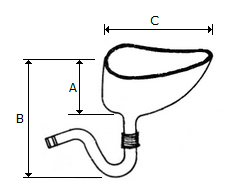
\includegraphics{../data_img/estimating-and-costing_1525417724-28.png}
}
\\\begin{enumerate*}[itemjoin=\qquad, label=\Alph*.]
\item{25 cm}
\item{30 cm}
\item{40 cm}
\item{45 cm}
\end{enumerate*}
\item{The value of 'C' of Indian type W.C. shown in the given figure is: \\

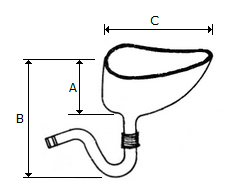
\includegraphics{../data_img/estimating-and-costing_1525417741-28.png}
}
\\\begin{enumerate*}[itemjoin=\qquad, label=\Alph*.]
\item{400 mm}
\item{450 mm}
\item{500 mm}
\item{550 mm}
\end{enumerate*}
\item{The value of 'B' of Indian type W.C. shown in the given figure is: \\

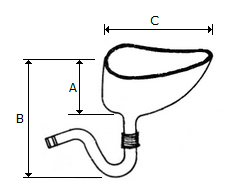
\includegraphics{../data_img/estimating-and-costing_1525417756-28.png}
}
\\\begin{enumerate*}[itemjoin=\qquad, label=\Alph*.]
\item{45 cm}
\item{50 cm}
\item{30 cm}
\item{25 cm}
\end{enumerate*}
\item{The area of the cross-section of a road fully in banking shown in the given figure, is \\

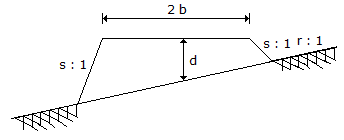
\includegraphics{../data_img/estimating-and-costing_1525417783-26.png}
}
\\\begin{enumerate*}[itemjoin=\qquad, label=\Alph*.]
\item{$ \frac{{{\text{s}}{{\text{b}}^2} + {{\text{r}}^2}{{\left( {2{\text{bd}} + {\text{sd}}} \right)}^2}}}{{{{\text{r}}^2} - {{\text{s}}^2}}} $}
\item{$ \frac{{{\text{s}}{{\text{b}}^2} + {{\text{r}}^2}{{\left( {2{\text{bd}} + {\text{sd}}} \right)}^2}}}{{{{\text{r}}^2} - {{\text{s}}^5}}} $}
\item{$ \frac{{{\text{s}}{{\text{b}}^2} + {{\text{r}}^2}{{\left( {2{\text{bd}} + {\text{sd}}} \right)}^2}}}{{{\text{r}} - {\text{s}}}} $}
\item{None of these}
\end{enumerate*}
\item{A cement concrete road is 1000 m long, 8 m wide and 15 cm thick over the sub-base of 10 cm thick gravel. The box cutting in road crust is}
\\\begin{enumerate*}[itemjoin=\qquad, label=\Alph*.]
\item{500 m\^{}3}
\item{1000 m\^{}3}
\item{1500 m\^{}3}
\item{2000 m\^{}3}
\end{enumerate*}
\item{The concrete work for the following part of the building of specified thickness is measured in square meters}
\\\begin{enumerate*}[itemjoin=\qquad, label=\Alph*.]
\item{Root slabs}
\item{Floors}
\item{Wall panels}
\item{All the above}
\end{enumerate*}
\item{The expected out turn of cement concrete 1 : 2 : 4 per mason per day is}
\\\begin{enumerate*}[itemjoin=\qquad, label=\Alph*.]
\item{1.5 m\^{}3}
\item{2.5 m\^{}3}
\item{3.5 m\^{}3}
\item{5.0 m\^{}3}
\end{enumerate*}
\item{The expected out turn of half brick partition wall per mason per day is}
\\\begin{enumerate*}[itemjoin=\qquad, label=\Alph*.]
\item{1.5 m\^{}2}
\item{2.0 m\^{}2}
\item{4.0 m\^{}2}
\item{5.0 m\^{}2}
\end{enumerate*}
\item{The measurement is made in square metre in case of}
\begin{enumerate}[label=\Alph*.]
\item{Cement concrete in foundation}
\item{R.C.C. structure}
\item{Hollow concrete block wall}
\item{None of these}
\end{enumerate}
\item{The measurement is made for stone work in square metre in case of}
\begin{enumerate}[label=\Alph*.]
\item{Wall facing}
\item{Columns, lintels, copings}
\item{Building work}
\item{(A) and (B) of the above}
\end{enumerate}
\item{As per Indian Standard Specifications, the peak discharge for domestic purposes per capita per minute, is taken}
\begin{enumerate}[label=\Alph*.]
\item{1.80 liters for 5 to 10 users}
\item{1.20 liters for 15 users}
\item{1.35 for 20 users}
\item{All the above}
\end{enumerate}
\item{Pick up the correct statement in case of water supply.}
\begin{enumerate}[label=\Alph*.]
\item{Pipes laid in trenches and pipes fixed to walls are measured separately}
\item{Cutting through walls and floors are included with the item}
\item{Pipes are classified according to their sizes and quality}
\item{All the above}
\end{enumerate}
\item{The cost of the earthwork in excavation for the surface drain of cross-section shown in the given figure for a total length of 5 metres @ Rs. 450\% cum, is \\

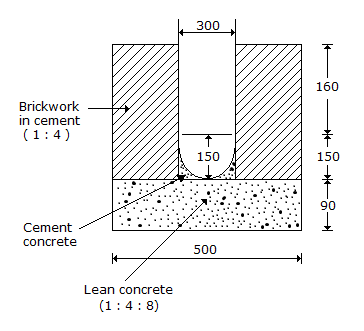
\includegraphics{../data_img/estimating-and-costing_1525417814-29.png}
}
\\\begin{enumerate*}[itemjoin=\qquad, label=\Alph*.]
\item{Rs. 400}
\item{Rs. 425}
\item{Rs. 450}
\item{Rs. 500}
\end{enumerate*}
\item{For the construction of buildings, the subheads of the estimate are}
\begin{enumerate}[label=\Alph*.]
\item{Earthwork, Concrete work, Brick work}
\item{Brickwork, Stone work, Roofing}
\item{Brickwork Flooring, Wood work, Steel work}
\item{All the above}
\end{enumerate}
\item{The damp proof course (D.P.C.) is measured in}
\\\begin{enumerate*}[itemjoin=\qquad, label=\Alph*.]
\item{Cub. m}
\item{Sq. m}
\item{Meters}
\item{None of these}
\end{enumerate*}
\item{The diameter of a domestic sewer pipe laid at gradient 1 in 100 is recommended}
\\\begin{enumerate*}[itemjoin=\qquad, label=\Alph*.]
\item{100 mm}
\item{150 mm}
\item{200 mm}
\item{175 mm}
\end{enumerate*}
\item{The area of a sloping surface of a protective embankment of mean height `d', side slopes S : 1 and length `L' is
}
\\\begin{enumerate*}[itemjoin=\qquad, label=\Alph*.]
\item{$ {\text{d}} \times {\text{d}} \times {\text{s}} $}
\item{$ \sqrt {{{\text{d}}^2} \times {\text{d}}{{\text{s}}^2}}  $}
\item{$ {\text{Ld}}\sqrt {1 + {{\text{s}}^2}}  $}
\item{$ 2{\text{Ld}}\sqrt {1 + {{\text{s}}^2}}  $}
\end{enumerate*}
\item{The detention period in a septic tank is assumed}
\\\begin{enumerate*}[itemjoin=\qquad, label=\Alph*.]
\item{20 minutes}
\item{25 minutes}
\item{30 minutes}
\item{40 minutes}
\end{enumerate*}
\item{Carpet area does not include the area of}
\begin{enumerate}[label=\Alph*.]
\item{The walls along with doors and other openings}
\item{Bath room and lavatory}
\item{Kitchen and pantry}
\item{None of the above}
\end{enumerate}
\item{While estimating the qualities for the construction of a building, the correct metric unit is}
\begin{enumerate}[label=\Alph*.]
\item{Meter for length}
\item{Cubic metre for area}
\item{Square meters for volume}
\item{Liter for capacity}
\end{enumerate}
\item{The volume is measured correct to the nearest}
\\\begin{enumerate*}[itemjoin=\qquad, label=\Alph*.]
\item{0.01 cum}
\item{0.02 cum}
\item{0.03 cum}
\item{0.04 cum}
\end{enumerate*}
\item{The area is measured correct to the nearest}
\\\begin{enumerate*}[itemjoin=\qquad, label=\Alph*.]
\item{0.01 sqm}
\item{0.02 sqm}
\item{0.03 sqm}
\item{0.04 sqm}
\end{enumerate*}
\item{While preparing a detailed estimate}
\begin{enumerate}[label=\Alph*.]
\item{Dimension should be measured correct to 0.01 m}
\item{Area should be measured correct to 0.01 sqm}
\item{Volume should be measured correct to 0.01 cum}
\item{All the above}
\end{enumerate}
\item{The plinth area of a building not includes}
\begin{enumerate}[label=\Alph*.]
\item{Area of the walls at the floor level}
\item{Internal shaft for sanitary installations up to 2 sq m. in area}
\item{Lift and wall including landing}
\item{Area of cantilevered porch}
\end{enumerate}
\item{In the mid-section formula}
\begin{enumerate}[label=\Alph*.]
\item{The mean depth is the average of depths of two consecutive sections}
\item{The area of mid-sections is calculated by using mean depth}
\item{The volume of the earth work is calculated by multiplying the mid-section area by the distance between the two original sections}
\item{All of the above}
\end{enumerate}
\item{The inspection pit or chamber is a manhole provided in a base drainage system}
\begin{enumerate}[label=\Alph*.]
\item{At every change of direction}
\item{At every change of gradient}
\item{At every 30 m intervals}
\item{All the above}
\end{enumerate}
\item{The cross-sectional area of the embankment of a canal fully in embankment in the given figure is \\

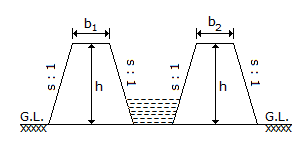
\includegraphics{../data_img/estimating-and-costing_1525417845-31.png}
}
\\\begin{enumerate*}[itemjoin=\qquad, label=\Alph*.]
\item{$ \frac{1}{2}\left( {{{\text{b}}_1} + {{\text{b}}_2}} \right){\text{h}} $}
\item{$ \left( {{{\text{b}}_1} + {{\text{b}}_2}} \right){\text{h}} + {\text{s}}{{\text{h}}^2} $}
\item{$ \left( {{{\text{b}}_1} + {{\text{b}}_2}} \right) + 2{\text{s}}{{\text{h}}^2} $}
\item{$ 2\left[ {\left( {{{\text{b}}_1} + {{\text{b}}_2}} \right)\left( {{\text{b}} + {\text{s}}{{\text{h}}^2}} \right)} \right] $}
\end{enumerate*}
\item{Anti-siphonage pipe is connected to}
\begin{enumerate}[label=\Alph*.]
\item{Main soil pipe}
\item{Bottom of P trap W.C.}
\item{Top of P trap W.C.}
\item{Side of water closet}
\end{enumerate}
\item{The 'centre line method' is specially adopted for estimating}
\begin{enumerate}[label=\Alph*.]
\item{Circular buildings}
\item{Hexagonal buildings}
\item{Octagonal buildings}
\item{All the above}
\end{enumerate}
\item{In long and short wall method of estimation, the length of long wall is the centre to centre distance between the walls and}
\begin{enumerate}[label=\Alph*.]
\item{Breadth of the wall}
\item{Half breadth of wall on each side}
\item{One fourth breadth of wall on each side}
\item{None of these}
\end{enumerate}
\item{According to ISI method of measurement, the order of the sequence is}
\begin{enumerate}[label=\Alph*.]
\item{Length, breadth, height}
\item{Breadth, length, height}
\item{Height, length, breadth}
\item{None of these}
\end{enumerate}
\item{The rate of an item of work depends on}
\begin{enumerate}[label=\Alph*.]
\item{Specifications of works}
\item{Specifications of materials}
\item{Proportion of mortar}
\item{All the above}
\end{enumerate}
\item{The cross-sections for a highway is taken at}
\begin{enumerate}[label=\Alph*.]
\item{Right angle to the centre line}
\item{30 meters apart}
\item{Intermediate points having abrupt change in gradient}
\item{All the above}
\end{enumerate}
\item{If tensile stress of a steel rod of diameter `D' is 1400 kg/cm\^{}2 and bond stress is 6 kg/cm\^{}2, the required bond length of the rod is
}
\\\begin{enumerate*}[itemjoin=\qquad, label=\Alph*.]
\item{30 D}
\item{39 D}
\item{50 D}
\item{59 D}
\end{enumerate*}
\item{The most reliable estimate is}
\begin{enumerate}[label=\Alph*.]
\item{Detailed estimate}
\item{Preliminary estimate}
\item{Plinth area estimate}
\item{Cube rate estimate}
\end{enumerate}
\item{The main factor to be considered while preparing a detailed estimate, is}
\begin{enumerate}[label=\Alph*.]
\item{Quantity of the materials}
\item{Availability of materials}
\item{Transportation of materials}
\item{All the above}
\end{enumerate}
\item{The order of booking dimensions is}
\begin{enumerate}[label=\Alph*.]
\item{Length, breadth, height}
\item{Breadth, length, height}
\item{Height, breadth, length}
\item{None of these}
\end{enumerate}
\item{The reduced levels of points, 30 metres apart along the longitudinal section of a road portion between chainages 5 and 9 are shown in the given figure. If there is a uniform up-gradient of the road 120 in 1, the chainage of the point with no filling or cutting is \\

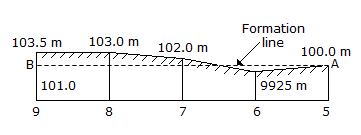
\includegraphics{../data_img/estimating-and-costing_1525417876-30.png}
}
\begin{enumerate}[label=\Alph*.]
\item{(6 + 15) chains}
\item{(6 + 12) chains}
\item{(6 + 18) chains}
\item{None of these}
\end{enumerate}
\item{The expected out turn of brick work in cement mortar in foundation and plinth per mason per day, is}
\\\begin{enumerate*}[itemjoin=\qquad, label=\Alph*.]
\item{1.00 m\^{}3}
\item{1.25 m\^{}3}
\item{1.50 m\^{}3}
\item{1.75 m\^{}3}
\end{enumerate*}
\item{Pick up the correct statement regarding the centre line method of estimating a building}
\begin{enumerate}[label=\Alph*.]
\item{Product of the centre line of the walls and area of cross-section of any item, gives total quantity of the item}
\item{The centre line is worked out separately for different sections of walls of a building}
\item{The centre line length is reduced by half the layer of main wall joining the partition wall}
\item{All the above}
\end{enumerate}
\item{For 12 mm thick cement plastering 1 : 6 on 100 sq.m new brick work, the quantity of cement required, is}
\\\begin{enumerate*}[itemjoin=\qquad, label=\Alph*.]
\item{0.200 m\^{}3}
\item{0.247 m\^{}3}
\item{0.274 m\^{}3}
\item{0.295 m\^{}3}
\end{enumerate*}
\item{For 100 sq. m cement concrete (1 : 2 : 4) 4 cm thick floor, the quantity of cement required, is}
\\\begin{enumerate*}[itemjoin=\qquad, label=\Alph*.]
\item{0.90 m\^{}3}
\item{0.94 m\^{}3}
\item{0.98 m\^{}3}
\item{1.00 m\^{}3}
\end{enumerate*}
\item{The measurement is not made in square meters in case of}
\begin{enumerate}[label=\Alph*.]
\item{D.P.C. (Damp proof course)}
\item{Form works}
\item{Concrete Jeffries}
\item{R.C. Chhajja}
\end{enumerate}
\item{The brick work is measured in sq metre, in case of}
\begin{enumerate}[label=\Alph*.]
\item{Honey comb brick work}
\item{Brick flat soling}
\item{Half brick walls or the partition}
\item{All the above}
\end{enumerate}
\item{According to Indian Standards Institute, the actual size of modular bricks is}
\begin{enumerate}[label=\Alph*.]
\item{23 cm $\times$ 11.5 cm $\times$ 7.5 cm}
\item{25 cm $\times$ 13 cm $\times$ 7.5 cm}
\item{19 cm $\times$ 9 cm $\times$ 9 cm}
\item{20 cm $\times$ 10 cm $\times$ 10 cm}
\end{enumerate}
\item{The brick work is not measured in cu m in case of}
\begin{enumerate}[label=\Alph*.]
\item{One or more than one brick wall}
\item{Brick work in arches}
\item{Reinforced brick work}
\item{Half brick wall}
\end{enumerate}
\item{Berms are provided in canals if these are}
\begin{enumerate}[label=\Alph*.]
\item{Fully in excavation}
\item{Partly in excavation and partly in embankment}
\item{Fully in embankment}
\item{All the above}
\end{enumerate}
\item{While estimating a reinforced cement structure, the omitted cover of concrete is assumed}
\begin{enumerate}[label=\Alph*.]
\item{At the end of reinforcing bar, not less than 25 mm or twice the diameter of the bar}
\item{In thin slabs, 12 mm minimum or diameter of the bar whichever is more}
\item{For reinforcing longitudinal bar in a beam 25 mm minimum or diameter of the largest bar which is more}
\item{All the above}
\end{enumerate}
\item{Pick up the item of work not included in the plinth area estimate}
\\\begin{enumerate*}[itemjoin=\qquad, label=\Alph*.]
\item{Wall thickness}
\item{Room area}
\item{W' Area}
\item{Courtyard area}
\end{enumerate*}
\item{The ground surface slopes 1 in 50 along a proposed railway embankment 150 m in length. The height of the embankment at zero chainage is 0.5 m, the width is 11 m and side slopes 2 : 1. If the falling gradient of the embankment is 1 in 150, the quantity of the earthwork calculated by Prismoidal formula, is}
\\\begin{enumerate*}[itemjoin=\qquad, label=\Alph*.]
\item{3250 m\^{}3}
\item{3225 m\^{}3}
\item{3275 m\^{}3}
\item{3300 m\^{}3}
\end{enumerate*}
\item{Pick up the correct statement from the following:}
\begin{enumerate}[label=\Alph*.]
\item{All pipes and fittings are classified according to their diameters}
\item{The diameter of the pipes is the nominal diameter of internal bore}
\item{All pipes are measured along the centre line of the pipes in meters}
\item{All the above}
\end{enumerate}
\item{Pick up the correct statement from the following:}
\begin{enumerate}[label=\Alph*.]
\item{Bricks are paid per thousand}
\item{Cement is paid per 50 kg bag}
\item{Lime is paid per quintal}
\item{All the above}
\end{enumerate}
\item{Pick up the incorrect statement from the following:}
\begin{enumerate}[label=\Alph*.]
\item{Dimensions are measured to the nearest 0.01 m}
\item{Areas are measured to the nearest 0.01 sq.m}
\item{Cubic contents are measured to the nearest 0.1 cum}
\item{Weights are measured to the nearest 0.001 tonnes}
\end{enumerate}
\item{Pick up the correct statement from the following:}
\begin{enumerate}[label=\Alph*.]
\item{If the bed level is above N.S.L. the canal is called fully in baking and the berms are designed as 3d where d is full supply depth of water (F.S.D.)}
\item{Area of canal in cutting = BD + Sd\^{}2 where B = bed width, d = depth of cutting and S is the side slope}
\item{Area of the bank of canal = B\_ 1d\_ 1 + Sd\_ 2 where B\_ 1, d\_ 1 and S are the width of bank, height of the bank above N.S.L. and side slope respectively}
\item{If F.S.L. is above N.S.L. the canal is called partly in cutting and partly in filling and berms are designed as 2d where d is full supply depth}
\item{All the above}
\end{enumerate}
\item{Pick up the correct statement from the following:}
\begin{enumerate}[label=\Alph*.]
\item{In a gully trap, a water seal of 6 to 7.5 cm is provided}
\item{The gully trap collects waste water from the kitchen, sink, wash basins, etc.}
\item{The gully trap disconnects the sullage drain from the main drainage system}
\item{The grating provided over gully traps is 23 cm square}
\end{enumerate}
\item{Pick up the correct statement from the following:}
\begin{enumerate}[label=\Alph*.]
\item{In order to check up the average depth of excavation, 'Dead man's' are left at the mid-widths of borrow pits}
\item{The earthwork calculation in excavation is made from the difference in levels obtained with a level}
\item{The earth work in excavation to form the road embankment includes the formation of correct profile and depositing the soil in layers}
\item{All the above}
\end{enumerate}
\item{Pick up the incorrect statement regarding a master trap from the following:}
\begin{enumerate}[label=\Alph*.]
\item{It is provided in between the lower end of the house drain and the street sewer}
\item{It is provided a cleaning eye at the top of the trap}
\item{The mica flap valve which opens inwards only, is fitted at the top of the inlet pipe}
\item{The water seal is less than that of ordinary traps}
\end{enumerate}
\item{Pick up the incorrect statement from the following:}
\begin{enumerate}[label=\Alph*.]
\item{Lead is the average horizontal straight distance between the borrow pit and the place of spreading soil}
\item{The lead is calculated for each block of the excavated area}
\item{The unit of lead is 50 m for a distance upto 500 m}
\item{The unit of lead is 1 km where the lead exceeds 2 km}
\end{enumerate}
\item{Pick up the incorrect statement from the following:}
\begin{enumerate}[label=\Alph*.]
\item{No deduction is made for the volume occupied by reinforcement}
\item{No deduction is made for the openings upto 0.1 sq.m}
\item{No deduction is made for volumes occupied by pipes, not exceeding 100 sq.cm in cross-section}
\item{None of these}
\end{enumerate}
\item{Pick up the correct statement from the following:}
\begin{enumerate}[label=\Alph*.]
\item{Pointing is measured in sq.m}
\item{Plastering is measured in sq.m}
\item{Glazing is measured in sq.m}
\item{All the above}
\end{enumerate}
\item{Pick up the correct statement from the following:}
\begin{enumerate}[label=\Alph*.]
\item{The bent up bars at a support resist the negative bending moment}
\item{The bent up bars at a support resist the sharing force}
\item{The bending of bars near supports is generally at 45$^\circ$}
\item{All the above}
\end{enumerate}
\item{Pick up the incorrect statement from the following:}
\begin{enumerate}[label=\Alph*.]
\item{The built up covered area at the floor level of any storey of a building is called plinth area}
\item{The usable covered area of the rooms of any storey of a building is called carpet area}
\item{The carpet area of a building along with area of its kitchen, pantry, store, lavatory, bath room and glazed veranda, is called floor area}
\item{None of these}
\end{enumerate}
\item{Pick up the correct statement from the following:}
\begin{enumerate}[label=\Alph*.]
\item{The earth work of cutting in trenches or borrow pits in fairly uniform ground is measured with the help of average depths of the dead men}
\item{The earth work in trenches or borrow pits in irregular ground is measured by taking the difference in levels before and after completion of work}
\item{The earth work in trenches or borrow pits, where neither a nor b is feasible, are measured from the fillings after deduction of voids}
\item{All the above}
\end{enumerate}
\end{enumerate}
\textbf{Answer Key}
\begin{tabular}{ | c | c c c c c c c c c c | }
\hline
 & 1 & 2 & 3 & 4 & 5 & 6 & 7 & 8 & 9 & 0 \\
\hline
0 & D & D & D & D & B & D & D & B & C & A \\
10 & A & D & D & D & D & D & D & D & D & C \\
20 & D & B & B & C & C & D & D & A & A & D \\
30 & D & D & D & C & C & D & B & A & D & D \\
40 & D & A & D & A & B & B & D & C & B & D \\
50 & D & C & D & B & D & D & B & D & D & C \\
60 & E & B & D & D & D & D & D & D & D & D \\
\hline
\end{tabular}
\clearpage
\subsection*{Section 2}
\begin{enumerate}
\item{Pick up the correct statement from the following:}
\begin{enumerate}[label=\Alph*.]
\item{The estimated value of the work excluding the amount for contingencies, work charged establishment, tool and plants, is called work value}
\item{The actual expenditure involved to complete a work including incidental, establishment and travelling charges, is called actual cost}
\item{The formal acceptance by the administrative department for incurring an expenditure on the work, is called administrative approval}
\item{All the above}
\end{enumerate}
\item{Pick up the correct statement from the following:}
\begin{enumerate}[label=\Alph*.]
\item{The incidental expenses of a miscellaneous character which could not be predicted during preparation of the estimate, is called contingencies}
\item{Additional supervising staff engaged at work site, is called work charged establishment}
\item{Detailed specifications specify qualities, quantities and the proportions of materials to be used for a particular item}
\item{All the above}
\end{enumerate}
\item{Referring of given figure, pick up the correct statement from the following: \\

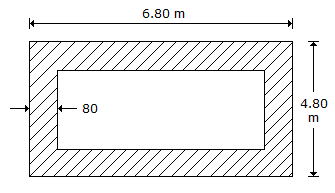
\includegraphics{../data_img/estimating-and-costing_1525417914-25.png}
}
\begin{enumerate}[label=\Alph*.]
\item{The total length of centre line of four walls is 20 m}
\item{Length of long wall out-to-out is 6.80 m}
\item{Length of short walls in-to-in is 3.20 m}
\item{All the above}
\end{enumerate}
\item{The height of the sink of wash basin above floor level is kept}
\\\begin{enumerate*}[itemjoin=\qquad, label=\Alph*.]
\item{60 cm}
\item{70 cm}
\item{75 cm to 80 cm}
\item{80 cm}
\end{enumerate*}
\item{The unit of measurement is per quintal for the following:}
\begin{enumerate}[label=\Alph*.]
\item{Collapsible gates with rails}
\item{Rolling shutters}
\item{Expanded metal wire netting}
\item{M.S. reinforcement of R.C.C. works}
\end{enumerate}
\item{The slope of the outlet of 'P trap' below the horizontal is kept}
\\\begin{enumerate*}[itemjoin=\qquad, label=\Alph*.]
\item{8$^\circ$}
\item{10$^\circ$}
\item{12$^\circ$}
\item{14$^\circ$}
\end{enumerate*}
\item{The expected out turn for earth work in excavation in ordinary soil per workman per day is}
\\\begin{enumerate*}[itemjoin=\qquad, label=\Alph*.]
\item{1.00 cum}
\item{2.00 cum}
\item{3.00 cum}
\item{4.00 cum}
\end{enumerate*}
\item{The weight of an item is measured correct to nearest}
\\\begin{enumerate*}[itemjoin=\qquad, label=\Alph*.]
\item{0.25 kg}
\item{0.50 kg}
\item{0.75 kg}
\item{1.00 kg}
\end{enumerate*}
\item{The expected out turn of 2.5 cm cement concrete floor per mansion per day}
\\\begin{enumerate*}[itemjoin=\qquad, label=\Alph*.]
\item{2.5 sqm}
\item{5.0 sqm}
\item{7.5 sqm}
\item{10 sqm}
\end{enumerate*}
\item{Cost of fittings and their fixing is specified for the following sanitary fittings}
\begin{enumerate}[label=\Alph*.]
\item{Water closets}
\item{Flushing pipes}
\item{Lavatory basins}
\item{All the above}
\end{enumerate}
\item{The cross-section of a road partly in banking and partly in cutting is shown in the given figure. The area of the shaded portion is \\

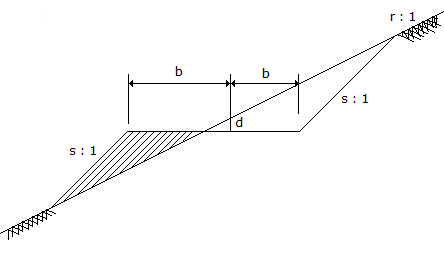
\includegraphics{../data_img/estimating-and-costing_1525417951-27.png}
}
\\\begin{enumerate*}[itemjoin=\qquad, label=\Alph*.]
\item{$ \frac{1}{3} \times \frac{{{{\left( {{\text{b}} - {\text{rd}}} \right)}^2}}}{{{\text{r}} - {\text{s}}}} $}
\item{$ \frac{1}{3} \times \frac{{{{\left( {{\text{b}} - {\text{rd}}} \right)}^2}}}{{{\text{r}} + {\text{s}}}} $}
\item{$ \frac{1}{2} \times \frac{{{{\left( {{\text{b}} + {\text{rd}}} \right)}^2}}}{{{\text{r}} - {\text{s}}}} $}
\item{$ \frac{1}{3} \times \frac{{{{\left( {{\text{b}} - {\text{rd}}} \right)}^2}}}{{{\text{s}} - {\text{r}}}} $}
\end{enumerate*}
\item{Pick up the item whose weight is added to the weight of respective item, is}
\\\begin{enumerate*}[itemjoin=\qquad, label=\Alph*.]
\item{Cleats}
\item{Brackets}
\item{Bolts}
\item{All the above}
\end{enumerate*}
\item{Brick walls are measured in sq. m if the thickness of the wall is}
\\\begin{enumerate*}[itemjoin=\qquad, label=\Alph*.]
\item{10 cm}
\item{15 cm}
\item{20 cm}
\item{None of these}
\end{enumerate*}
\item{The item of steel work which is measured in sq.m, is}
\begin{enumerate}[label=\Alph*.]
\item{Collapsible gates}
\item{Rolling shutters}
\item{Ventilators and glazing}
\item{All the above}
\end{enumerate}
\item{The item of the brick structure measured in sq.m, is}
\begin{enumerate}[label=\Alph*.]
\item{Reinforced brick work}
\item{Broken glass coping}
\item{Brick edging}
\item{Brick work in arches}
\end{enumerate}
\item{The following item of earth work is not measured separately.}
\begin{enumerate}[label=\Alph*.]
\item{Setting out of works}
\item{Site clearance}
\item{Steps in deep excavation}
\item{All the above}
\end{enumerate}
\item{The trap which is provided to disconnect the house drain from the street sewer is called}
\begin{enumerate}[label=\Alph*.]
\item{Master trap}
\item{Intercepting trap}
\item{Interception manhole}
\item{All the above}
\end{enumerate}
\item{Pick up the excavation where measurements are made in square meters for payment.}
\begin{enumerate}[label=\Alph*.]
\item{Ordinary cuttings up to 1 m}
\item{Surface dressing up to 15 cm depths}
\item{Surface excavation up to 30 cm depths}
\item{Both (B) and (C)}
\end{enumerate}
\item{A portion of an embankment having a uniform up-gradient 1 in 500 is circular with radius 1000 m of the centre line. It subtends 180$^\circ$ at the centre. If the height of the bank is 1 m at the lower end, and side slopes 2 : 1, the earth work involved.
}
\\\begin{enumerate*}[itemjoin=\qquad, label=\Alph*.]
\item{26,000 m\^{}3}
\item{26,500 m\^{}3}
\item{27,000 m\^{}3}
\item{27,500 m\^{}3}
\end{enumerate*}
\item{The floor area includes the area of the balcony up to}
\\\begin{enumerate*}[itemjoin=\qquad, label=\Alph*.]
\item{100 \%}
\item{75 \%}
\item{50 \%}
\item{25 \%}
\end{enumerate*}
\item{In case of laying gullies, siphons, intercepting traps, the cost includes}
\begin{enumerate}[label=\Alph*.]
\item{Setting and laying}
\item{Bed concreting}
\item{Connection to drains}
\item{All of these}
\end{enumerate}
\item{The minimum width of a septic tank is taken}
\\\begin{enumerate*}[itemjoin=\qquad, label=\Alph*.]
\item{70 cm}
\item{75 cm}
\item{80 cm}
\item{90 cm}
\end{enumerate*}
\item{The total length of a cranked bar through a distance (d) at 45$^\circ$ in case of a beam of effective length L, is
}
\begin{enumerate}[label=\Alph*.]
\item{L + 0.42 d}
\item{L + (2 $\times$ 0.42 d)}
\item{L - (0.42 d)}
\item{L - (2 $\times$ 0.4 d)}
\end{enumerate}
\item{The correct Prismoidal formula for volume is}
\\\begin{enumerate*}[itemjoin=\qquad, label=\Alph*.]
\item{$ {\text{D}}$$ [first area + last area + \sum Even area + 2 \sum odd area $}
\item{$ \frac{{\text{D}}}{3}$$ [first area + last area + 4 \sum Even area + 2 \sum odd area $}
\item{$ \frac{{\text{D}}}{3}$$ [first area + last area + 2 \sum Even area + 4 \sum odd area $}
\item{$ \frac{{\text{D}}}{6}$$ [first area + last area + 2 \sum Even area + 4 \sum odd area $}
\end{enumerate*}
\item{The assumption on which the trapezoidal formula for volumes is based, is}
\begin{enumerate}[label=\Alph*.]
\item{The end sections are parallel planes}
\item{The mid-area of a pyramid is half the average area of the ends}
\item{The volume of the Prismoidal is over-estimated and hence a Prismoidal correction is applied}
\item{All the above}
\end{enumerate}
\end{enumerate}
\textbf{Answer Key}
\begin{tabular}{ | c | c c c c c c c c c c | }
\hline
 & 1 & 2 & 3 & 4 & 5 & 6 & 7 & 8 & 9 & 0 \\
\hline
0 & D & D & D & C & D & D & C & D & C & D \\
10 & A & D & A & D & B & D & D & D & D & C \\
20 & D & B & B & B & D &   &   &   &   &   \\
\hline
\end{tabular}
\end{document}